\documentclass[twoside]{book}

% Packages required by doxygen
\usepackage{fixltx2e}
\usepackage{calc}
\usepackage{doxygen}
\usepackage[export]{adjustbox} % also loads graphicx
\usepackage{graphicx}
\usepackage[utf8]{inputenc}
\usepackage{makeidx}
\usepackage{multicol}
\usepackage{multirow}
\PassOptionsToPackage{warn}{textcomp}
\usepackage{textcomp}
\usepackage[nointegrals]{wasysym}
\usepackage[table]{xcolor}

% Font selection
\usepackage[T1]{fontenc}
\usepackage[scaled=.90]{helvet}
\usepackage{courier}
\usepackage{amssymb}
\usepackage{sectsty}
\renewcommand{\familydefault}{\sfdefault}
\allsectionsfont{%
  \fontseries{bc}\selectfont%
  \color{darkgray}%
}
\renewcommand{\DoxyLabelFont}{%
  \fontseries{bc}\selectfont%
  \color{darkgray}%
}
\newcommand{\+}{\discretionary{\mbox{\scriptsize$\hookleftarrow$}}{}{}}

% Page & text layout
\usepackage{geometry}
\geometry{%
  a4paper,%
  top=2.5cm,%
  bottom=2.5cm,%
  left=2.5cm,%
  right=2.5cm%
}
\tolerance=750
\hfuzz=15pt
\hbadness=750
\setlength{\emergencystretch}{15pt}
\setlength{\parindent}{0cm}
\setlength{\parskip}{3ex plus 2ex minus 2ex}
\makeatletter
\renewcommand{\paragraph}{%
  \@startsection{paragraph}{4}{0ex}{-1.0ex}{1.0ex}{%
    \normalfont\normalsize\bfseries\SS@parafont%
  }%
}
\renewcommand{\subparagraph}{%
  \@startsection{subparagraph}{5}{0ex}{-1.0ex}{1.0ex}{%
    \normalfont\normalsize\bfseries\SS@subparafont%
  }%
}
\makeatother

% Headers & footers
\usepackage{fancyhdr}
\pagestyle{fancyplain}
\fancyhead[LE]{\fancyplain{}{\bfseries\thepage}}
\fancyhead[CE]{\fancyplain{}{}}
\fancyhead[RE]{\fancyplain{}{\bfseries\leftmark}}
\fancyhead[LO]{\fancyplain{}{\bfseries\rightmark}}
\fancyhead[CO]{\fancyplain{}{}}
\fancyhead[RO]{\fancyplain{}{\bfseries\thepage}}
\fancyfoot[LE]{\fancyplain{}{}}
\fancyfoot[CE]{\fancyplain{}{}}
\fancyfoot[RE]{\fancyplain{}{\bfseries\scriptsize Generated by Doxygen }}
\fancyfoot[LO]{\fancyplain{}{\bfseries\scriptsize Generated by Doxygen }}
\fancyfoot[CO]{\fancyplain{}{}}
\fancyfoot[RO]{\fancyplain{}{}}
\renewcommand{\footrulewidth}{0.4pt}
\renewcommand{\chaptermark}[1]{%
  \markboth{#1}{}%
}
\renewcommand{\sectionmark}[1]{%
  \markright{\thesection\ #1}%
}

% Indices & bibliography
\usepackage{natbib}
\usepackage[titles]{tocloft}
\setcounter{tocdepth}{3}
\setcounter{secnumdepth}{5}
\makeindex

% Hyperlinks (required, but should be loaded last)
\usepackage{ifpdf}
\ifpdf
  \usepackage[pdftex,pagebackref=true]{hyperref}
\else
  \usepackage[ps2pdf,pagebackref=true]{hyperref}
\fi
\hypersetup{%
  colorlinks=true,%
  linkcolor=blue,%
  citecolor=blue,%
  unicode%
}

% Custom commands
\newcommand{\clearemptydoublepage}{%
  \newpage{\pagestyle{empty}\cleardoublepage}%
}

\usepackage{caption}
\captionsetup{labelsep=space,justification=centering,font={bf},singlelinecheck=off,skip=4pt,position=top}

%===== C O N T E N T S =====

\begin{document}

% Titlepage & ToC
\hypersetup{pageanchor=false,
             bookmarksnumbered=true,
             pdfencoding=unicode
            }
\pagenumbering{roman}
\begin{titlepage}
\vspace*{7cm}
\begin{center}%
{\Large Rebar Addon for Free\+C\+AD }\\
\vspace*{1cm}
{\large Generated by Doxygen 1.8.11}\\
\end{center}
\end{titlepage}
\clearemptydoublepage
\tableofcontents
\clearemptydoublepage
\pagenumbering{arabic}
\hypersetup{pageanchor=true}

%--- Begin generated contents ---
\chapter{Rebar Addon for Free\+C\+AD}
\label{index}\hypertarget{index}{}Started as a Google Summer of Code (\href{https://en.wikipedia.org/wiki/Google_Summer_of_Code}{\tt G\+SoC} 2017) \href{https://summerofcode.withgoogle.com/archive/2017/projects/6536382147198976}{\tt project}.



\subsection*{Documentation}

This project is aimed at easing up the process of rebaring in \href{https://www.freecadweb.org}{\tt Free\+C\+AD}. In this project, list of rebars will be provided to user under Rebar tools in the form of dropdown. This project covers six different rebar shapes as given below\+:


\begin{DoxyItemize}
\item  {\bfseries Straight Rebar}\+: \href{https://www.freecadweb.org/wiki/Arch_Rebar_Straight}{\tt wiki} 
\item  {\bfseries U\+Shape Rebar}\+: \href{https://www.freecadweb.org/wiki/Arch_Rebar_UShape}{\tt wiki} 
\item  {\bfseries L\+Shape Rebar}\+: \href{https://www.freecadweb.org/wiki/Arch_Rebar_LShape}{\tt wiki} 
\item  {\bfseries Bent\+Shpae Rebar}\+: \href{https://www.freecadweb.org/wiki/Arch_Rebar_BentShape}{\tt wiki} 
\item  {\bfseries \hyperlink{namespaceStirrup}{Stirrup} Rebar}\+: \href{https://www.freecadweb.org/wiki/Arch_Rebar_Stirrup}{\tt wiki} 
\item  {\bfseries Helical Rebar}\+: \href{https://www.freecadweb.org/wiki/Arch_Rebar_Helical}{\tt wiki} 
\end{DoxyItemize}

\subsection*{Video Tutorial}

\href{https://www.youtube.com/watch?v=BYQQjEKmx5E&t=1435s}{\tt }

\subsection*{Installation}

\subsubsection*{Pre-\/requisites}


\begin{DoxyItemize}
\item Free\+C\+AD (version $>$= 0.\+17)\+: \href{https://www.freecadweb.org/wiki/Installing}{\tt Installation guide}
\end{DoxyItemize}

\subsubsection*{Steps to install Rebar Addon in Free\+C\+AD}


\begin{DoxyEnumerate}
\item Open the Free\+C\+AD Addon Manager ({\ttfamily Tool -\/$>$ Addon manager}).
\item When an addon manager will open, select {\ttfamily Reinforcement} from a list of workbenches shown by an addon manager.
\item After selecting, click on {\ttfamily Install/\+Update} button.
\item Restart Free\+C\+AD.
\item Now you will see different rebars in a drop-\/down list of rebar tools ({\ttfamily Arch -\/$>$ Rebar tools -\/$>$ Different rebars}).
\end{DoxyEnumerate}

\subsection*{How it works}

Each rebar tool has two files, one is {\ttfamily Python} file and second is there respective name {\ttfamily UI} file like {\ttfamily \hyperlink{StraightRebar_8py}{Straight\+Rebar.\+py}} and {\ttfamily Straight\+Rebar.\+ui} file). Let\textquotesingle{}s take a straight rebar tool. In {\ttfamily \hyperlink{StraightRebar_8py}{Straight\+Rebar.\+py}} file, there are two functions. One is {\ttfamily \hyperlink{namespaceStraightRebar_af6270367d7beae457813e33718d80faf}{make\+Straight\+Rebar()}} function. This function creates straight rebar and adds new properties to the default {\ttfamily Rebar} object. Second function is {\ttfamily edit\+Straight\+Rebar}. This function is used when we want to change a new properties(which is created by {\ttfamily make\+Straight\+Rebar} function) of the rebar object and it will take {\ttfamily Rebar} object as input which is created by {\ttfamily make\+Straight\+Rebar} function. In {\ttfamily \hyperlink{StraightRebar_8py}{Straight\+Rebar.\+py}}, {\ttfamily \+\_\+\+Straight\+Rebar\+Task\+Panel} class is present. This class loads UI(present in {\ttfamily Striaght\+Rebar.\+ui} file) in the task panel of Free\+C\+AD. First time when a user clicks on {\ttfamily Apply} or {\ttfamily Ok} button, then {\ttfamily make\+Straight\+Rebar} function is executed and after that when user want to change the properties of Straight rebar then {\ttfamily edit\+Straight\+Rebar} function is excuted.

\subsection*{Extras}


\begin{DoxyItemize}
\item \href{https://forum.freecadweb.org/viewtopic.php?f=8&t=22760}{\tt Free\+C\+AD forum thread}
\item \href{https://brlcad.org/wiki/User:Amritpal_singh/gsoc_proposal}{\tt G\+SoC proposal}
\item \href{https://brlcad.org/wiki/User:Amritpal_singh/GSoC17/logs}{\tt Development logs} 
\end{DoxyItemize}
\chapter{Namespace Index}
\section{Namespace List}
Here is a list of all namespaces with brief descriptions\+:\begin{DoxyCompactList}
\item\contentsline{section}{\hyperlink{namespaceBentShapeRebar}{Bent\+Shape\+Rebar} }{\pageref{namespaceBentShapeRebar}}{}
\item\contentsline{section}{\hyperlink{namespaceHelicalRebar}{Helical\+Rebar} }{\pageref{namespaceHelicalRebar}}{}
\item\contentsline{section}{\hyperlink{namespaceLShapeRebar}{L\+Shape\+Rebar} }{\pageref{namespaceLShapeRebar}}{}
\item\contentsline{section}{\hyperlink{namespacePopUpImage}{Pop\+Up\+Image} }{\pageref{namespacePopUpImage}}{}
\item\contentsline{section}{\hyperlink{namespaceRebarDistribution}{Rebar\+Distribution} }{\pageref{namespaceRebarDistribution}}{}
\item\contentsline{section}{\hyperlink{namespaceRebarfunc}{Rebarfunc} }{\pageref{namespaceRebarfunc}}{}
\item\contentsline{section}{\hyperlink{namespaceRebarTools}{Rebar\+Tools} }{\pageref{namespaceRebarTools}}{}
\item\contentsline{section}{\hyperlink{namespaceStirrup}{Stirrup} }{\pageref{namespaceStirrup}}{}
\item\contentsline{section}{\hyperlink{namespaceStraightRebar}{Straight\+Rebar} }{\pageref{namespaceStraightRebar}}{}
\item\contentsline{section}{\hyperlink{namespaceUShapeRebar}{U\+Shape\+Rebar} }{\pageref{namespaceUShapeRebar}}{}
\end{DoxyCompactList}

\chapter{Hierarchical Index}
\section{Class Hierarchy}
This inheritance list is sorted roughly, but not completely, alphabetically\+:\begin{DoxyCompactList}
\item \contentsline{section}{Bent\+Shape\+Rebar.\+\_\+\+Bent\+Shape\+Rebar\+Task\+Panel}{\pageref{classBentShapeRebar_1_1__BentShapeRebarTaskPanel}}{}
\item \contentsline{section}{Helical\+Rebar.\+\_\+\+Helical\+Rebar\+Task\+Panel}{\pageref{classHelicalRebar_1_1__HelicalRebarTaskPanel}}{}
\item \contentsline{section}{L\+Shape\+Rebar.\+\_\+\+L\+Shape\+Rebar\+Task\+Panel}{\pageref{classLShapeRebar_1_1__LShapeRebarTaskPanel}}{}
\item \contentsline{section}{Rebar\+Distribution.\+\_\+\+Rebar\+Distribution\+Dialog}{\pageref{classRebarDistribution_1_1__RebarDistributionDialog}}{}
\item \contentsline{section}{Stirrup.\+\_\+\+Stirrup\+Task\+Panel}{\pageref{classStirrup_1_1__StirrupTaskPanel}}{}
\item \contentsline{section}{Straight\+Rebar.\+\_\+\+Straight\+Rebar\+Task\+Panel}{\pageref{classStraightRebar_1_1__StraightRebarTaskPanel}}{}
\item \contentsline{section}{U\+Shape\+Rebar.\+\_\+\+U\+Shape\+Rebar\+Task\+Panel}{\pageref{classUShapeRebar_1_1__UShapeRebarTaskPanel}}{}
\item \contentsline{section}{Rebar\+Tools.\+Bent\+Shape\+Rebar\+Tool}{\pageref{classRebarTools_1_1BentShapeRebarTool}}{}
\item \contentsline{section}{Rebar\+Tools.\+Helical\+Rebar\+Tool}{\pageref{classRebarTools_1_1HelicalRebarTool}}{}
\item \contentsline{section}{Rebar\+Tools.\+L\+Shape\+Rebar\+Tool}{\pageref{classRebarTools_1_1LShapeRebarTool}}{}
\item Q\+Dialog\begin{DoxyCompactList}
\item \contentsline{section}{Pop\+Up\+Image.\+Pop\+Up\+Image}{\pageref{classPopUpImage_1_1PopUpImage}}{}
\end{DoxyCompactList}
\item \contentsline{section}{Rebar\+Tools.\+Stirrup\+Tool}{\pageref{classRebarTools_1_1StirrupTool}}{}
\item \contentsline{section}{Rebar\+Tools.\+Straight\+Rebar\+Tool}{\pageref{classRebarTools_1_1StraightRebarTool}}{}
\item \contentsline{section}{Rebar\+Tools.\+U\+Shape\+Rebar\+Tool}{\pageref{classRebarTools_1_1UShapeRebarTool}}{}
\end{DoxyCompactList}

\chapter{Class Index}
\section{Class List}
Here are the classes, structs, unions and interfaces with brief descriptions\+:\begin{DoxyCompactList}
\item\contentsline{section}{\hyperlink{classBentShapeRebar_1_1__BentShapeRebarTaskPanel}{Bent\+Shape\+Rebar.\+\_\+\+Bent\+Shape\+Rebar\+Task\+Panel} }{\pageref{classBentShapeRebar_1_1__BentShapeRebarTaskPanel}}{}
\item\contentsline{section}{\hyperlink{classHelicalRebar_1_1__HelicalRebarTaskPanel}{Helical\+Rebar.\+\_\+\+Helical\+Rebar\+Task\+Panel} }{\pageref{classHelicalRebar_1_1__HelicalRebarTaskPanel}}{}
\item\contentsline{section}{\hyperlink{classLShapeRebar_1_1__LShapeRebarTaskPanel}{L\+Shape\+Rebar.\+\_\+\+L\+Shape\+Rebar\+Task\+Panel} }{\pageref{classLShapeRebar_1_1__LShapeRebarTaskPanel}}{}
\item\contentsline{section}{\hyperlink{classRebarDistribution_1_1__RebarDistributionDialog}{Rebar\+Distribution.\+\_\+\+Rebar\+Distribution\+Dialog} }{\pageref{classRebarDistribution_1_1__RebarDistributionDialog}}{}
\item\contentsline{section}{\hyperlink{classStirrup_1_1__StirrupTaskPanel}{Stirrup.\+\_\+\+Stirrup\+Task\+Panel} }{\pageref{classStirrup_1_1__StirrupTaskPanel}}{}
\item\contentsline{section}{\hyperlink{classStraightRebar_1_1__StraightRebarTaskPanel}{Straight\+Rebar.\+\_\+\+Straight\+Rebar\+Task\+Panel} }{\pageref{classStraightRebar_1_1__StraightRebarTaskPanel}}{}
\item\contentsline{section}{\hyperlink{classUShapeRebar_1_1__UShapeRebarTaskPanel}{U\+Shape\+Rebar.\+\_\+\+U\+Shape\+Rebar\+Task\+Panel} }{\pageref{classUShapeRebar_1_1__UShapeRebarTaskPanel}}{}
\item\contentsline{section}{\hyperlink{classRebarTools_1_1BentShapeRebarTool}{Rebar\+Tools.\+Bent\+Shape\+Rebar\+Tool} }{\pageref{classRebarTools_1_1BentShapeRebarTool}}{}
\item\contentsline{section}{\hyperlink{classRebarTools_1_1HelicalRebarTool}{Rebar\+Tools.\+Helical\+Rebar\+Tool} }{\pageref{classRebarTools_1_1HelicalRebarTool}}{}
\item\contentsline{section}{\hyperlink{classRebarTools_1_1LShapeRebarTool}{Rebar\+Tools.\+L\+Shape\+Rebar\+Tool} }{\pageref{classRebarTools_1_1LShapeRebarTool}}{}
\item\contentsline{section}{\hyperlink{classPopUpImage_1_1PopUpImage}{Pop\+Up\+Image.\+Pop\+Up\+Image} }{\pageref{classPopUpImage_1_1PopUpImage}}{}
\item\contentsline{section}{\hyperlink{classRebarTools_1_1StirrupTool}{Rebar\+Tools.\+Stirrup\+Tool} }{\pageref{classRebarTools_1_1StirrupTool}}{}
\item\contentsline{section}{\hyperlink{classRebarTools_1_1StraightRebarTool}{Rebar\+Tools.\+Straight\+Rebar\+Tool} }{\pageref{classRebarTools_1_1StraightRebarTool}}{}
\item\contentsline{section}{\hyperlink{classRebarTools_1_1UShapeRebarTool}{Rebar\+Tools.\+U\+Shape\+Rebar\+Tool} }{\pageref{classRebarTools_1_1UShapeRebarTool}}{}
\end{DoxyCompactList}

\chapter{File Index}
\section{File List}
Here is a list of all files with brief descriptions\+:\begin{DoxyCompactList}
\item\contentsline{section}{\hyperlink{BentShapeRebar_8py}{Bent\+Shape\+Rebar.\+py} }{\pageref{BentShapeRebar_8py}}{}
\item\contentsline{section}{\hyperlink{HelicalRebar_8py}{Helical\+Rebar.\+py} }{\pageref{HelicalRebar_8py}}{}
\item\contentsline{section}{\hyperlink{LShapeRebar_8py}{L\+Shape\+Rebar.\+py} }{\pageref{LShapeRebar_8py}}{}
\item\contentsline{section}{\hyperlink{PopUpImage_8py}{Pop\+Up\+Image.\+py} }{\pageref{PopUpImage_8py}}{}
\item\contentsline{section}{\hyperlink{RebarDistribution_8py}{Rebar\+Distribution.\+py} }{\pageref{RebarDistribution_8py}}{}
\item\contentsline{section}{\hyperlink{Rebarfunc_8py}{Rebarfunc.\+py} }{\pageref{Rebarfunc_8py}}{}
\item\contentsline{section}{\hyperlink{RebarTools_8py}{Rebar\+Tools.\+py} }{\pageref{RebarTools_8py}}{}
\item\contentsline{section}{\hyperlink{Stirrup_8py}{Stirrup.\+py} }{\pageref{Stirrup_8py}}{}
\item\contentsline{section}{\hyperlink{StraightRebar_8py}{Straight\+Rebar.\+py} }{\pageref{StraightRebar_8py}}{}
\item\contentsline{section}{\hyperlink{UShapeRebar_8py}{U\+Shape\+Rebar.\+py} }{\pageref{UShapeRebar_8py}}{}
\end{DoxyCompactList}

\chapter{Namespace Documentation}
\hypertarget{namespaceBentShapeRebar}{}\section{Bent\+Shape\+Rebar Namespace Reference}
\label{namespaceBentShapeRebar}\index{Bent\+Shape\+Rebar@{Bent\+Shape\+Rebar}}
\subsection*{Classes}
\begin{DoxyCompactItemize}
\item 
class \hyperlink{classBentShapeRebar_1_1__BentShapeRebarTaskPanel}{\+\_\+\+Bent\+Shape\+Rebar\+Task\+Panel}
\end{DoxyCompactItemize}
\subsection*{Functions}
\begin{DoxyCompactItemize}
\item 
def \hyperlink{namespaceBentShapeRebar_a33951a8ab21a73bae42af9f81d7c43c3}{getpoints\+Of\+Bent\+Shape\+Rebar} (Face\+P\+RM, l\+\_\+cover, r\+\_\+cover, b\+\_\+cover, t\+\_\+cover, bent\+Length, bent\+Angle, orientation)
\item 
def \hyperlink{namespaceBentShapeRebar_aac46779d3e1905db5a3788917f6e2476}{make\+Bent\+Shape\+Rebar} (f\+\_\+cover, b\+\_\+cover, l\+\_\+cover, r\+\_\+cover, diameter, t\+\_\+cover, bent\+Length, bent\+Angle, rounding, amount\+\_\+spacing\+\_\+check, amount\+\_\+spacing\+\_\+value, orientation=\char`\"{}Bottom Left\char`\"{}, structure=None, facename=None)
\item 
def \hyperlink{namespaceBentShapeRebar_a941d005845cd497c0beb12bb8fef9171}{edit\+Bent\+Shape\+Rebar} (Rebar, f\+\_\+cover, b\+\_\+cover, l\+\_\+cover, r\+\_\+cover, diameter, t\+\_\+cover, bent\+Length, bent\+Angle, rounding, amount\+\_\+spacing\+\_\+check, amount\+\_\+spacing\+\_\+value, orientation, structure=None, facename=None)
\item 
def \hyperlink{namespaceBentShapeRebar_ae5db82a49148a0a8f6fa567fa72d93b2}{edit\+Dialog} (vobj)
\item 
def \hyperlink{namespaceBentShapeRebar_abc4f0ada7811da5cf9174551bc3c6b37}{Command\+Bent\+Shape\+Rebar} ()
\end{DoxyCompactItemize}
\subsection*{Variables}
\begin{DoxyCompactItemize}
\item 
string \hyperlink{namespaceBentShapeRebar_a38b223debc1826fd2855773a02749bb4}{\+\_\+\+\_\+title\+\_\+\+\_\+} = \char`\"{}Bent\+Shape\+Rebar\char`\"{}
\item 
string \hyperlink{namespaceBentShapeRebar_ad79a2dbf88601c24aae561033cb48d34}{\+\_\+\+\_\+author\+\_\+\+\_\+} = \char`\"{}Amritpal Singh\char`\"{}
\item 
string \hyperlink{namespaceBentShapeRebar_aec768ca6a259d1cc738ea11c79a124e2}{\+\_\+\+\_\+url\+\_\+\+\_\+} = \char`\"{}https\+://www.\+freecadweb.\+org\char`\"{}
\end{DoxyCompactItemize}


\subsection{Function Documentation}
\index{Bent\+Shape\+Rebar@{Bent\+Shape\+Rebar}!Command\+Bent\+Shape\+Rebar@{Command\+Bent\+Shape\+Rebar}}
\index{Command\+Bent\+Shape\+Rebar@{Command\+Bent\+Shape\+Rebar}!Bent\+Shape\+Rebar@{Bent\+Shape\+Rebar}}
\subsubsection[{\texorpdfstring{Command\+Bent\+Shape\+Rebar()}{CommandBentShapeRebar()}}]{\setlength{\rightskip}{0pt plus 5cm}def Bent\+Shape\+Rebar.\+Command\+Bent\+Shape\+Rebar (
\begin{DoxyParamCaption}
{}
\end{DoxyParamCaption}
)}\hypertarget{namespaceBentShapeRebar_abc4f0ada7811da5cf9174551bc3c6b37}{}\label{namespaceBentShapeRebar_abc4f0ada7811da5cf9174551bc3c6b37}


Definition at line \hyperlink{BentShapeRebar_8py_source_l00359}{359} of file \hyperlink{BentShapeRebar_8py_source}{Bent\+Shape\+Rebar.\+py}.


\begin{DoxyCode}
\hypertarget{namespaceBentShapeRebar.tex_l00359}{}\hyperlink{namespaceBentShapeRebar_abc4f0ada7811da5cf9174551bc3c6b37}{00359} \textcolor{keyword}{def }\hyperlink{namespaceBentShapeRebar_abc4f0ada7811da5cf9174551bc3c6b37}{CommandBentShapeRebar}():
00360     selected\_obj = \hyperlink{namespaceRebarfunc_adae2713855a7e1b4bda04081ae671542}{check\_selected\_face}()
00361     \textcolor{keywordflow}{if} selected\_obj:
00362         FreeCADGui.Control.showDialog(\hyperlink{classBentShapeRebar_1_1__BentShapeRebarTaskPanel}{\_BentShapeRebarTaskPanel}())
00363 \end{DoxyCode}


Here is the call graph for this function\+:\nopagebreak
\begin{figure}[H]
\begin{center}
\leavevmode
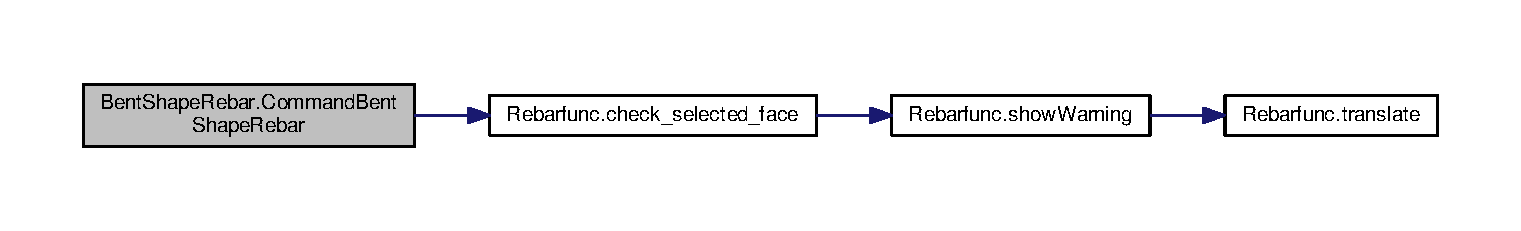
\includegraphics[width=350pt]{namespaceBentShapeRebar_abc4f0ada7811da5cf9174551bc3c6b37_cgraph}
\end{center}
\end{figure}




Here is the caller graph for this function\+:\nopagebreak
\begin{figure}[H]
\begin{center}
\leavevmode
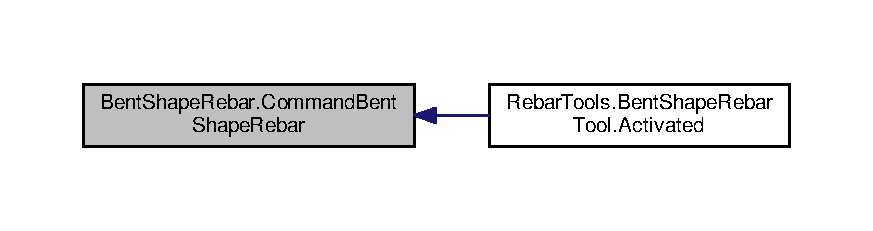
\includegraphics[width=350pt]{namespaceBentShapeRebar_abc4f0ada7811da5cf9174551bc3c6b37_icgraph}
\end{center}
\end{figure}


\index{Bent\+Shape\+Rebar@{Bent\+Shape\+Rebar}!edit\+Bent\+Shape\+Rebar@{edit\+Bent\+Shape\+Rebar}}
\index{edit\+Bent\+Shape\+Rebar@{edit\+Bent\+Shape\+Rebar}!Bent\+Shape\+Rebar@{Bent\+Shape\+Rebar}}
\subsubsection[{\texorpdfstring{edit\+Bent\+Shape\+Rebar(\+Rebar, f\+\_\+cover, b\+\_\+cover, l\+\_\+cover, r\+\_\+cover, diameter, t\+\_\+cover, bent\+Length, bent\+Angle, rounding, amount\+\_\+spacing\+\_\+check, amount\+\_\+spacing\+\_\+value, orientation, structure=\+None, facename=\+None)}{editBentShapeRebar(Rebar, f_cover, b_cover, l_cover, r_cover, diameter, t_cover, bentLength, bentAngle, rounding, amount_spacing_check, amount_spacing_value, orientation, structure=None, facename=None)}}]{\setlength{\rightskip}{0pt plus 5cm}def Bent\+Shape\+Rebar.\+edit\+Bent\+Shape\+Rebar (
\begin{DoxyParamCaption}
\item[{}]{Rebar, }
\item[{}]{f\+\_\+cover, }
\item[{}]{b\+\_\+cover, }
\item[{}]{l\+\_\+cover, }
\item[{}]{r\+\_\+cover, }
\item[{}]{diameter, }
\item[{}]{t\+\_\+cover, }
\item[{}]{bent\+Length, }
\item[{}]{bent\+Angle, }
\item[{}]{rounding, }
\item[{}]{amount\+\_\+spacing\+\_\+check, }
\item[{}]{amount\+\_\+spacing\+\_\+value, }
\item[{}]{orientation, }
\item[{}]{structure = {\ttfamily None}, }
\item[{}]{facename = {\ttfamily None}}
\end{DoxyParamCaption}
)}\hypertarget{namespaceBentShapeRebar_a941d005845cd497c0beb12bb8fef9171}{}\label{namespaceBentShapeRebar_a941d005845cd497c0beb12bb8fef9171}


Definition at line \hyperlink{BentShapeRebar_8py_source_l00270}{270} of file \hyperlink{BentShapeRebar_8py_source}{Bent\+Shape\+Rebar.\+py}.


\begin{DoxyCode}
\hypertarget{namespaceBentShapeRebar.tex_l00270}{}\hyperlink{namespaceBentShapeRebar_a941d005845cd497c0beb12bb8fef9171}{00270} \textcolor{keyword}{def }\hyperlink{namespaceBentShapeRebar_a941d005845cd497c0beb12bb8fef9171}{editBentShapeRebar}(Rebar, f\_cover, b\_cover, l\_cover, r\_cover, diameter, t\_cover, 
      bentLength, bentAngle, rounding, amount\_spacing\_check, amount\_spacing\_value, orientation, structure = None, 
      facename = None):
00271     sketch = Rebar.Base
00272     \textcolor{keywordflow}{if} structure \textcolor{keywordflow}{and} facename:
00273         sketch.Support = [(structure, facename)]
00274     \textcolor{comment}{# Check if sketch support is empty.}
00275     \textcolor{keywordflow}{if} \textcolor{keywordflow}{not} sketch.Support:
00276         \hyperlink{namespaceRebarfunc_a2278a0602d46a62953af1fcf2e574a94}{showWarning}(\textcolor{stringliteral}{"You have checked remove external geometry of base sketchs when needed.\(\backslash\)nTo
       unchecked Edit->Preferences->Arch."})
00277         \textcolor{keywordflow}{return}
00278     \textcolor{comment}{# Assigned values}
00279     facename = sketch.Support[0][1][0]
00280     structure = sketch.Support[0][0]
00281     face = structure.Shape.Faces[\hyperlink{namespaceRebarfunc_a3885b3b63e3a41508ac79bc7550cf301}{getFaceNumber}(facename) - 1]
00282     \textcolor{comment}{#StructurePRM = getTrueParametersOfStructure(structure)}
00283     \textcolor{comment}{# Get parameters of the face where sketch of rebar is drawn}
00284     FacePRM = \hyperlink{namespaceRebarfunc_a92122b3d7cedd3d47bb63380a5ac4d08}{getParametersOfFace}(structure, facename)
00285     \textcolor{comment}{# Get points of L-Shape rebar}
00286     points = \hyperlink{namespaceBentShapeRebar_a33951a8ab21a73bae42af9f81d7c43c3}{getpointsOfBentShapeRebar}(FacePRM, l\_cover, r\_cover, b\_cover, t\_cover
      , bentLength, bentAngle, orientation)
00287     sketch.movePoint(0, 1, points[0], 0)
00288     FreeCAD.ActiveDocument.recompute()
00289     sketch.movePoint(0, 2, points[1], 0)
00290     FreeCAD.ActiveDocument.recompute()
00291     sketch.movePoint(1, 1, points[1], 0)
00292     FreeCAD.ActiveDocument.recompute()
00293     sketch.movePoint(1, 2, points[2], 0)
00294     FreeCAD.ActiveDocument.recompute()
00295 
00296     sketch.movePoint(2, 1, points[2], 0)
00297     FreeCAD.ActiveDocument.recompute()
00298     sketch.movePoint(2, 2, points[3], 0)
00299     FreeCAD.ActiveDocument.recompute()
00300     sketch.movePoint(3, 1, points[3], 0)
00301     FreeCAD.ActiveDocument.recompute()
00302     sketch.movePoint(3, 2, points[4], 0)
00303     FreeCAD.ActiveDocument.recompute()
00304 
00305     sketch.movePoint(4, 1, points[4], 0)
00306     FreeCAD.ActiveDocument.recompute()
00307     sketch.movePoint(4, 2, points[5], 0)
00308     FreeCAD.ActiveDocument.recompute()
00309 
00310     Rebar.OffsetStart = f\_cover
00311     Rebar.OffsetEnd = f\_cover
00312     \textcolor{keywordflow}{if} amount\_spacing\_check:
00313         Rebar.Amount = amount\_spacing\_value
00314         FreeCAD.ActiveDocument.recompute()
00315         Rebar.AmountCheck = \textcolor{keyword}{True}
00316     \textcolor{keywordflow}{else}:
00317         size = (ArchCommands.projectToVector(structure.Shape.copy(), face.normalAt(0, 0))).Length
00318         Rebar.Amount = int((size - diameter) / amount\_spacing\_value)
00319         FreeCAD.ActiveDocument.recompute()
00320         Rebar.AmountCheck = \textcolor{keyword}{False}
00321     Rebar.Diameter = diameter
00322     Rebar.FrontCover = f\_cover
00323     Rebar.LeftCover = l\_cover
00324     Rebar.RightCover = r\_cover
00325     Rebar.BottomCover = b\_cover
00326     Rebar.TopCover = t\_cover
00327     Rebar.BentLength = bentLength
00328     Rebar.BentAngle = bentAngle
00329     Rebar.Rounding = rounding
00330     Rebar.TrueSpacing = amount\_spacing\_value
00331     Rebar.Orientation = orientation
00332     FreeCAD.ActiveDocument.recompute()
00333     \textcolor{keywordflow}{return} Rebar
00334 
\end{DoxyCode}


Here is the call graph for this function\+:\nopagebreak
\begin{figure}[H]
\begin{center}
\leavevmode
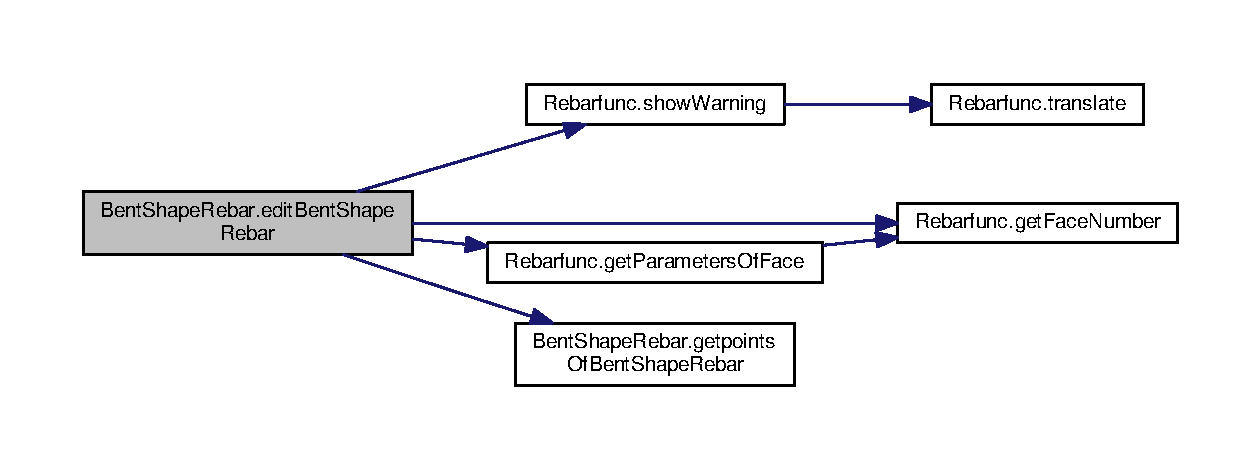
\includegraphics[width=350pt]{namespaceBentShapeRebar_a941d005845cd497c0beb12bb8fef9171_cgraph}
\end{center}
\end{figure}




Here is the caller graph for this function\+:\nopagebreak
\begin{figure}[H]
\begin{center}
\leavevmode
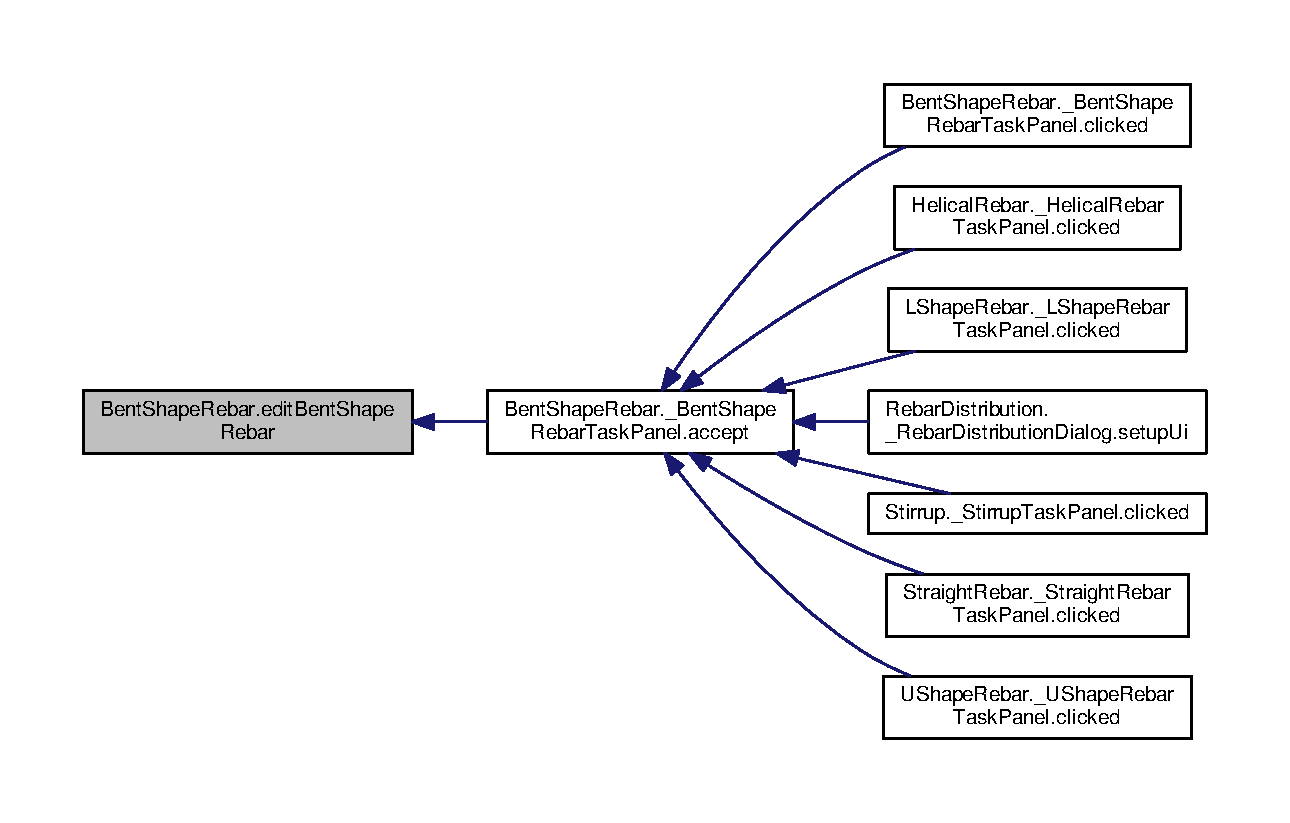
\includegraphics[width=350pt]{namespaceBentShapeRebar_a941d005845cd497c0beb12bb8fef9171_icgraph}
\end{center}
\end{figure}


\index{Bent\+Shape\+Rebar@{Bent\+Shape\+Rebar}!edit\+Dialog@{edit\+Dialog}}
\index{edit\+Dialog@{edit\+Dialog}!Bent\+Shape\+Rebar@{Bent\+Shape\+Rebar}}
\subsubsection[{\texorpdfstring{edit\+Dialog(vobj)}{editDialog(vobj)}}]{\setlength{\rightskip}{0pt plus 5cm}def Bent\+Shape\+Rebar.\+edit\+Dialog (
\begin{DoxyParamCaption}
\item[{}]{vobj}
\end{DoxyParamCaption}
)}\hypertarget{namespaceBentShapeRebar_ae5db82a49148a0a8f6fa567fa72d93b2}{}\label{namespaceBentShapeRebar_ae5db82a49148a0a8f6fa567fa72d93b2}


Definition at line \hyperlink{BentShapeRebar_8py_source_l00335}{335} of file \hyperlink{BentShapeRebar_8py_source}{Bent\+Shape\+Rebar.\+py}.


\begin{DoxyCode}
\hypertarget{namespaceBentShapeRebar.tex_l00335}{}\hyperlink{namespaceBentShapeRebar_ae5db82a49148a0a8f6fa567fa72d93b2}{00335} \textcolor{keyword}{def }\hyperlink{namespaceBentShapeRebar_ae5db82a49148a0a8f6fa567fa72d93b2}{editDialog}(vobj):
00336     FreeCADGui.Control.closeDialog()
00337     obj = \hyperlink{classBentShapeRebar_1_1__BentShapeRebarTaskPanel}{\_BentShapeRebarTaskPanel}(vobj.Object)
00338     obj.form.frontCover.setText(str(vobj.Object.FrontCover))
00339     obj.form.l\_sideCover.setText(str(vobj.Object.LeftCover))
00340     obj.form.r\_sideCover.setText(str(vobj.Object.RightCover))
00341     obj.form.bottomCover.setText(str(vobj.Object.BottomCover))
00342     obj.form.diameter.setText(str(vobj.Object.Diameter))
00343     obj.form.topCover.setText(str(vobj.Object.TopCover))
00344     obj.form.bentLength.setText(str(vobj.Object.BentLength))
00345     obj.form.bentAngle.setValue(vobj.Object.BentAngle)
00346     obj.form.rounding.setValue(vobj.Object.Rounding)
00347     obj.form.orientation.setCurrentIndex(obj.form.orientation.findText(str(vobj.Object.Orientation)))
00348     \textcolor{keywordflow}{if} vobj.Object.AmountCheck:
00349         obj.form.amount.setValue(vobj.Object.Amount)
00350     \textcolor{keywordflow}{else}:
00351         obj.form.amount\_radio.setChecked(\textcolor{keyword}{False})
00352         obj.form.spacing\_radio.setChecked(\textcolor{keyword}{True})
00353         obj.form.amount.setDisabled(\textcolor{keyword}{True})
00354         obj.form.spacing.setEnabled(\textcolor{keyword}{True})
00355         obj.form.spacing.setText(str(vobj.Object.TrueSpacing))
00356     \textcolor{comment}{#obj.form.PickSelectedFace.setVisible(False)}
00357     FreeCADGui.Control.showDialog(obj)
00358 
\end{DoxyCode}
\index{Bent\+Shape\+Rebar@{Bent\+Shape\+Rebar}!getpoints\+Of\+Bent\+Shape\+Rebar@{getpoints\+Of\+Bent\+Shape\+Rebar}}
\index{getpoints\+Of\+Bent\+Shape\+Rebar@{getpoints\+Of\+Bent\+Shape\+Rebar}!Bent\+Shape\+Rebar@{Bent\+Shape\+Rebar}}
\subsubsection[{\texorpdfstring{getpoints\+Of\+Bent\+Shape\+Rebar(\+Face\+P\+R\+M, l\+\_\+cover, r\+\_\+cover, b\+\_\+cover, t\+\_\+cover, bent\+Length, bent\+Angle, orientation)}{getpointsOfBentShapeRebar(FacePRM, l_cover, r_cover, b_cover, t_cover, bentLength, bentAngle, orientation)}}]{\setlength{\rightskip}{0pt plus 5cm}def Bent\+Shape\+Rebar.\+getpoints\+Of\+Bent\+Shape\+Rebar (
\begin{DoxyParamCaption}
\item[{}]{Face\+P\+RM, }
\item[{}]{l\+\_\+cover, }
\item[{}]{r\+\_\+cover, }
\item[{}]{b\+\_\+cover, }
\item[{}]{t\+\_\+cover, }
\item[{}]{bent\+Length, }
\item[{}]{bent\+Angle, }
\item[{}]{orientation}
\end{DoxyParamCaption}
)}\hypertarget{namespaceBentShapeRebar_a33951a8ab21a73bae42af9f81d7c43c3}{}\label{namespaceBentShapeRebar_a33951a8ab21a73bae42af9f81d7c43c3}
\begin{DoxyVerb}getpointsOfBentShapeRebar(FacePRM, LeftCover, RightCover, BottomCover, TopCover, BentLength, BentAngle, Orientation):
Return points of the LShape rebar in the form of array for sketch.
It takes four different orientations input i.e. 'Bottom', 'Top', 'Left', 'Right'.
\end{DoxyVerb}
 

Definition at line \hyperlink{BentShapeRebar_8py_source_l00040}{40} of file \hyperlink{BentShapeRebar_8py_source}{Bent\+Shape\+Rebar.\+py}.


\begin{DoxyCode}
\hypertarget{namespaceBentShapeRebar.tex_l00040}{}\hyperlink{namespaceBentShapeRebar_a33951a8ab21a73bae42af9f81d7c43c3}{00040} \textcolor{keyword}{def }\hyperlink{namespaceBentShapeRebar_a33951a8ab21a73bae42af9f81d7c43c3}{getpointsOfBentShapeRebar}(FacePRM, l\_cover, r\_cover, b\_cover, t\_cover, 
      bentLength, bentAngle, orientation):
00041     \textcolor{stringliteral}{""" getpointsOfBentShapeRebar(FacePRM, LeftCover, RightCover, BottomCover, TopCover, BentLength,
       BentAngle, Orientation):}
00042 \textcolor{stringliteral}{    Return points of the LShape rebar in the form of array for sketch.}
00043 \textcolor{stringliteral}{    It takes four different orientations input i.e. 'Bottom', 'Top', 'Left', 'Right'.}
00044 \textcolor{stringliteral}{    """}
00045     \textcolor{keywordflow}{if} orientation == \textcolor{stringliteral}{"Bottom"}:
00046         x1 = FacePRM[1][0] - FacePRM[0][0] / 2 + l\_cover
00047         y1 = FacePRM[1][1] + FacePRM[0][1] / 2 - t\_cover
00048         x2 = x1 + bentLength
00049         y2 = y1
00050         dis = (FacePRM[0][1] - t\_cover - b\_cover) * math.tan(math.radians(bentAngle - 90))
00051         x3 = x2 + dis
00052         y3 = FacePRM[1][1] - FacePRM[0][1] / 2 + b\_cover
00053         x4 = FacePRM[1][0] + FacePRM[0][0] / 2 - r\_cover - bentLength - dis
00054         y4 = y3
00055         x5 = x4 + dis
00056         y5 = y2
00057         x6 = x5 + bentLength
00058         y6 = y5
00059     \textcolor{keywordflow}{elif} orientation == \textcolor{stringliteral}{"Top"}:
00060         x1 = FacePRM[1][0] - FacePRM[0][0] / 2 + l\_cover
00061         y1 = FacePRM[1][1] - FacePRM[0][1] / 2 + b\_cover
00062         x2 = x1 + bentLength
00063         y2 = y1
00064         dis = (FacePRM[0][1] - t\_cover - b\_cover) * math.tan(math.radians(bentAngle - 90))
00065         x3 = x2 + dis
00066         y3 = FacePRM[1][1] + FacePRM[0][1] / 2 - t\_cover
00067         x4 = FacePRM[1][0] + FacePRM[0][0] / 2 - r\_cover - bentLength - dis
00068         y4 = y3
00069         x5 = x4 + dis
00070         y5 = y2
00071         x6 = x5 + bentLength
00072         y6 = y5
00073     \textcolor{keywordflow}{elif} orientation == \textcolor{stringliteral}{"Left"}:
00074         x1 = FacePRM[1][0] + FacePRM[0][0] / 2 - r\_cover
00075         y1 = FacePRM[1][1] + FacePRM[0][1] / 2 - t\_cover
00076         x2 = x1
00077         y2 = y1 - bentLength
00078         dis = (FacePRM[0][0] - r\_cover - l\_cover) * math.tan(math.radians(bentAngle - 90))
00079         x3 = FacePRM[1][0] - FacePRM[0][0] / 2 + l\_cover
00080         y3 = y2 - dis
00081         x4 = x3
00082         y4 = FacePRM[1][1] - FacePRM[0][1] / 2 + b\_cover + bentLength + dis
00083         x5 = x2
00084         y5 = y4 - dis
00085         x6 = x5
00086         y6 = y5 - bentLength
00087     \textcolor{keywordflow}{elif} orientation == \textcolor{stringliteral}{"Right"}:
00088         x1 = FacePRM[1][0] - FacePRM[0][0] / 2 + l\_cover
00089         y1 = FacePRM[1][1] + FacePRM[0][1] / 2 - t\_cover
00090         x2 = x1
00091         y2 = y1 - bentLength
00092         dis = (FacePRM[0][0] - r\_cover - l\_cover) * math.tan(math.radians(bentAngle - 90))
00093         x3 = FacePRM[1][0] + FacePRM[0][0] / 2 - r\_cover
00094         y3 = y2 - dis
00095         x4 = x3
00096         y4 = FacePRM[1][1] - FacePRM[0][1] / 2 + b\_cover + bentLength + dis
00097         x5 = x2
00098         y5 = y4 - dis
00099         x6 = x5
00100         y6 = y5 - bentLength
00101     \textcolor{keywordflow}{return} [FreeCAD.Vector(x1, y1, 0), FreeCAD.Vector(x2, y2, 0),\(\backslash\)
00102            FreeCAD.Vector(x3, y3, 0), FreeCAD.Vector(x4, y4, 0),\(\backslash\)
00103            FreeCAD.Vector(x5, y5, 0), FreeCAD.Vector(x6, y6, 0)]
00104 
\end{DoxyCode}


Here is the caller graph for this function\+:\nopagebreak
\begin{figure}[H]
\begin{center}
\leavevmode
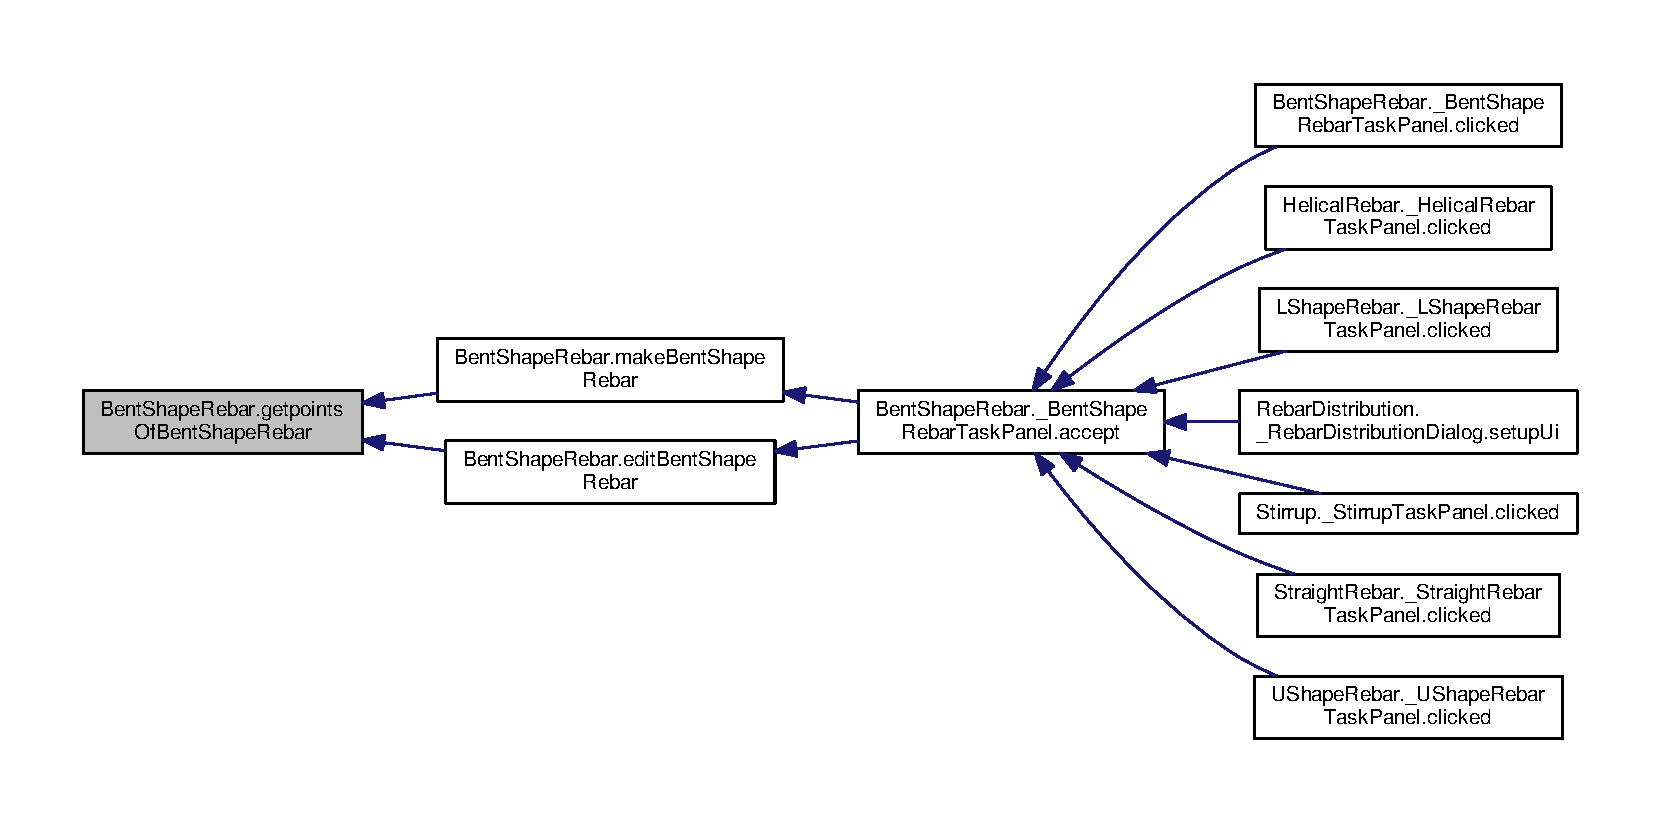
\includegraphics[width=350pt]{namespaceBentShapeRebar_a33951a8ab21a73bae42af9f81d7c43c3_icgraph}
\end{center}
\end{figure}


\index{Bent\+Shape\+Rebar@{Bent\+Shape\+Rebar}!make\+Bent\+Shape\+Rebar@{make\+Bent\+Shape\+Rebar}}
\index{make\+Bent\+Shape\+Rebar@{make\+Bent\+Shape\+Rebar}!Bent\+Shape\+Rebar@{Bent\+Shape\+Rebar}}
\subsubsection[{\texorpdfstring{make\+Bent\+Shape\+Rebar(f\+\_\+cover, b\+\_\+cover, l\+\_\+cover, r\+\_\+cover, diameter, t\+\_\+cover, bent\+Length, bent\+Angle, rounding, amount\+\_\+spacing\+\_\+check, amount\+\_\+spacing\+\_\+value, orientation=""Bottom Left"", structure=\+None, facename=\+None)}{makeBentShapeRebar(f_cover, b_cover, l_cover, r_cover, diameter, t_cover, bentLength, bentAngle, rounding, amount_spacing_check, amount_spacing_value, orientation="Bottom Left", structure=None, facename=None)}}]{\setlength{\rightskip}{0pt plus 5cm}def Bent\+Shape\+Rebar.\+make\+Bent\+Shape\+Rebar (
\begin{DoxyParamCaption}
\item[{}]{f\+\_\+cover, }
\item[{}]{b\+\_\+cover, }
\item[{}]{l\+\_\+cover, }
\item[{}]{r\+\_\+cover, }
\item[{}]{diameter, }
\item[{}]{t\+\_\+cover, }
\item[{}]{bent\+Length, }
\item[{}]{bent\+Angle, }
\item[{}]{rounding, }
\item[{}]{amount\+\_\+spacing\+\_\+check, }
\item[{}]{amount\+\_\+spacing\+\_\+value, }
\item[{}]{orientation = {\ttfamily \char`\"{}Bottom~Left\char`\"{}}, }
\item[{}]{structure = {\ttfamily None}, }
\item[{}]{facename = {\ttfamily None}}
\end{DoxyParamCaption}
)}\hypertarget{namespaceBentShapeRebar_aac46779d3e1905db5a3788917f6e2476}{}\label{namespaceBentShapeRebar_aac46779d3e1905db5a3788917f6e2476}
\begin{DoxyVerb}makeBentShapeRebar(FrontCover, BottomCover, LeftCover, RightCover, Diameter, TopCover, BentLength, BentAngle, Rounding,
AmountSpacingCheck, AmountSpacingValue, Orientation, Structure, Facename): Adds the Bent-Shape reinforcement bar to the
selected structural object.
It takes four different orientations input i.e. 'Bottom', 'Top', 'Left', 'Right'.
\end{DoxyVerb}
 

Definition at line \hyperlink{BentShapeRebar_8py_source_l00200}{200} of file \hyperlink{BentShapeRebar_8py_source}{Bent\+Shape\+Rebar.\+py}.


\begin{DoxyCode}
\hypertarget{namespaceBentShapeRebar.tex_l00200}{}\hyperlink{namespaceBentShapeRebar_aac46779d3e1905db5a3788917f6e2476}{00200} \textcolor{keyword}{def }\hyperlink{namespaceBentShapeRebar_aac46779d3e1905db5a3788917f6e2476}{makeBentShapeRebar}(f\_cover, b\_cover, l\_cover, r\_cover, diameter, t\_cover, bentLength,
       bentAngle, rounding, amount\_spacing\_check, amount\_spacing\_value, orientation = "Bottom Left", structure = 
      None, facename = None):
00201     \textcolor{stringliteral}{""" makeBentShapeRebar(FrontCover, BottomCover, LeftCover, RightCover, Diameter, TopCover, BentLength,
       BentAngle, Rounding,}
00202 \textcolor{stringliteral}{    AmountSpacingCheck, AmountSpacingValue, Orientation, Structure, Facename): Adds the Bent-Shape
       reinforcement bar to the}
00203 \textcolor{stringliteral}{    selected structural object.}
00204 \textcolor{stringliteral}{    It takes four different orientations input i.e. 'Bottom', 'Top', 'Left', 'Right'.}
00205 \textcolor{stringliteral}{    """}
00206     \textcolor{keywordflow}{if} \textcolor{keywordflow}{not} structure \textcolor{keywordflow}{and} \textcolor{keywordflow}{not} facename:
00207         selected\_obj = FreeCADGui.Selection.getSelectionEx()[0]
00208         structure = selected\_obj.Object
00209         facename = selected\_obj.SubElementNames[0]
00210     face = structure.Shape.Faces[\hyperlink{namespaceRebarfunc_a3885b3b63e3a41508ac79bc7550cf301}{getFaceNumber}(facename) - 1]
00211     \textcolor{comment}{#StructurePRM = getTrueParametersOfStructure(structure)}
00212     FacePRM = \hyperlink{namespaceRebarfunc_a92122b3d7cedd3d47bb63380a5ac4d08}{getParametersOfFace}(structure, facename)
00213     \textcolor{keywordflow}{if} \textcolor{keywordflow}{not} FacePRM:
00214         FreeCAD.Console.PrintError(\textcolor{stringliteral}{"Cannot identified shape or from which base object sturctural element is
       derived\(\backslash\)n"})
00215         \textcolor{keywordflow}{return}
00216     \textcolor{comment}{# Get points of L-Shape rebar}
00217     points = \hyperlink{namespaceBentShapeRebar_a33951a8ab21a73bae42af9f81d7c43c3}{getpointsOfBentShapeRebar}(FacePRM, l\_cover, r\_cover, b\_cover, t\_cover
      , bentLength, bentAngle, orientation)
00218     \textcolor{keyword}{import} Part
00219     \textcolor{keyword}{import} Arch
00220     sketch = FreeCAD.activeDocument().addObject(\textcolor{stringliteral}{'Sketcher::SketchObject'}, \textcolor{stringliteral}{'Sketch'})
00221     sketch.MapMode = \textcolor{stringliteral}{"FlatFace"}
00222     sketch.Support = [(structure, facename)]
00223     FreeCAD.ActiveDocument.recompute()
00224     sketch.addGeometry(Part.LineSegment(points[0], points[1]), \textcolor{keyword}{False})
00225     sketch.addGeometry(Part.LineSegment(points[1], points[2]), \textcolor{keyword}{False})
00226     sketch.addGeometry(Part.LineSegment(points[2], points[3]), \textcolor{keyword}{False})
00227     sketch.addGeometry(Part.LineSegment(points[3], points[4]), \textcolor{keyword}{False})
00228     sketch.addGeometry(Part.LineSegment(points[4], points[5]), \textcolor{keyword}{False})
00229     \textcolor{keyword}{import} Sketcher
00230     \textcolor{keywordflow}{if} amount\_spacing\_check:
00231         rebar = Arch.makeRebar(structure, sketch, diameter, amount\_spacing\_value, f\_cover)
00232         FreeCAD.ActiveDocument.recompute()
00233     \textcolor{keywordflow}{else}:
00234         size = (ArchCommands.projectToVector(structure.Shape.copy(), face.normalAt(0, 0))).Length
00235         rebar = Arch.makeRebar(structure, sketch, diameter, int((size - diameter) / amount\_spacing\_value), 
      f\_cover)
00236     rebar.Rounding = rounding
00237     \textcolor{comment}{# Adds properties to the rebar object}
00238     rebar.ViewObject.addProperty(\textcolor{stringliteral}{"App::PropertyString"}, \textcolor{stringliteral}{"RebarShape"}, \textcolor{stringliteral}{"RebarDialog"}, QT\_TRANSLATE\_NOOP(\textcolor{stringliteral}{"
      App::Property"}, \textcolor{stringliteral}{"Shape of rebar"})).RebarShape = \textcolor{stringliteral}{"BentShapeRebar"}
00239     rebar.ViewObject.setEditorMode(\textcolor{stringliteral}{"RebarShape"}, 2)
00240     rebar.addProperty(\textcolor{stringliteral}{"App::PropertyDistance"}, \textcolor{stringliteral}{"FrontCover"}, \textcolor{stringliteral}{"RebarDialog"}, QT\_TRANSLATE\_NOOP(\textcolor{stringliteral}{"
      App::Property"}, \textcolor{stringliteral}{"Front cover of rebar"})).FrontCover = f\_cover
00241     rebar.setEditorMode(\textcolor{stringliteral}{"FrontCover"}, 2)
00242     rebar.addProperty(\textcolor{stringliteral}{"App::PropertyDistance"}, \textcolor{stringliteral}{"LeftCover"}, \textcolor{stringliteral}{"RebarDialog"}, QT\_TRANSLATE\_NOOP(\textcolor{stringliteral}{"App::Property
      "}, \textcolor{stringliteral}{"Left Side cover of rebar"})).LeftCover = l\_cover
00243     rebar.setEditorMode(\textcolor{stringliteral}{"LeftCover"}, 2)
00244     rebar.addProperty(\textcolor{stringliteral}{"App::PropertyDistance"}, \textcolor{stringliteral}{"RightCover"}, \textcolor{stringliteral}{"RebarDialog"}, QT\_TRANSLATE\_NOOP(\textcolor{stringliteral}{"
      App::Property"}, \textcolor{stringliteral}{"Right Side cover of rebar"})).RightCover = r\_cover
00245     rebar.setEditorMode(\textcolor{stringliteral}{"RightCover"}, 2)
00246     rebar.addProperty(\textcolor{stringliteral}{"App::PropertyDistance"}, \textcolor{stringliteral}{"BottomCover"}, \textcolor{stringliteral}{"RebarDialog"}, QT\_TRANSLATE\_NOOP(\textcolor{stringliteral}{"
      App::Property"}, \textcolor{stringliteral}{"Bottom cover of rebar"})).BottomCover = b\_cover
00247     rebar.setEditorMode(\textcolor{stringliteral}{"BottomCover"}, 2)
00248     rebar.addProperty(\textcolor{stringliteral}{"App::PropertyBool"}, \textcolor{stringliteral}{"AmountCheck"}, \textcolor{stringliteral}{"RebarDialog"}, QT\_TRANSLATE\_NOOP(\textcolor{stringliteral}{"App::Property"},
       \textcolor{stringliteral}{"Amount radio button is checked"})).AmountCheck
00249     rebar.setEditorMode(\textcolor{stringliteral}{"AmountCheck"}, 2)
00250     rebar.addProperty(\textcolor{stringliteral}{"App::PropertyDistance"}, \textcolor{stringliteral}{"TopCover"}, \textcolor{stringliteral}{"RebarDialog"}, QT\_TRANSLATE\_NOOP(\textcolor{stringliteral}{"App::Property"}
      , \textcolor{stringliteral}{"Top cover of rebar"})).TopCover = t\_cover
00251     rebar.setEditorMode(\textcolor{stringliteral}{"TopCover"}, 2)
00252     rebar.addProperty(\textcolor{stringliteral}{"App::PropertyDistance"}, \textcolor{stringliteral}{"TrueSpacing"}, \textcolor{stringliteral}{"RebarDialog"}, QT\_TRANSLATE\_NOOP(\textcolor{stringliteral}{"
      App::Property"}, \textcolor{stringliteral}{"Spacing between of rebars"})).TrueSpacing = amount\_spacing\_value
00253     rebar.addProperty(\textcolor{stringliteral}{"App::PropertyString"}, \textcolor{stringliteral}{"Orientation"}, \textcolor{stringliteral}{"RebarDialog"}, QT\_TRANSLATE\_NOOP(\textcolor{stringliteral}{"App::Property
      "}, \textcolor{stringliteral}{"Shape of rebar"})).Orientation = orientation
00254     rebar.setEditorMode(\textcolor{stringliteral}{"Orientation"}, 2)
00255     rebar.setEditorMode(\textcolor{stringliteral}{"TrueSpacing"}, 2)
00256     rebar.addProperty(\textcolor{stringliteral}{"App::PropertyDistance"}, \textcolor{stringliteral}{"BentLength"}, \textcolor{stringliteral}{"RebarDialog"}, QT\_TRANSLATE\_NOOP(\textcolor{stringliteral}{"
      App::Property"}, \textcolor{stringliteral}{"BentLength cover of rebar"})).BentLength = bentLength
00257     rebar.setEditorMode(\textcolor{stringliteral}{"BentLength"}, 2)
00258     rebar.addProperty(\textcolor{stringliteral}{"App::PropertyDistance"}, \textcolor{stringliteral}{"BentAngle"}, \textcolor{stringliteral}{"RebarDialog"}, QT\_TRANSLATE\_NOOP(\textcolor{stringliteral}{"App::Property
      "}, \textcolor{stringliteral}{"Bent Angle of rebar"})).BentAngle = bentAngle
00259     rebar.setEditorMode(\textcolor{stringliteral}{"BentAngle"}, 2)
00260 
00261     \textcolor{keywordflow}{if} amount\_spacing\_check:
00262         rebar.AmountCheck = \textcolor{keyword}{True}
00263     \textcolor{keywordflow}{else}:
00264         rebar.AmountCheck = \textcolor{keyword}{False}
00265         rebar.TrueSpacing = amount\_spacing\_value
00266     rebar.Label = \textcolor{stringliteral}{"BentShapeRebar"}
00267     FreeCAD.ActiveDocument.recompute()
00268     \textcolor{keywordflow}{return} rebar
00269 
\end{DoxyCode}


Here is the call graph for this function\+:\nopagebreak
\begin{figure}[H]
\begin{center}
\leavevmode
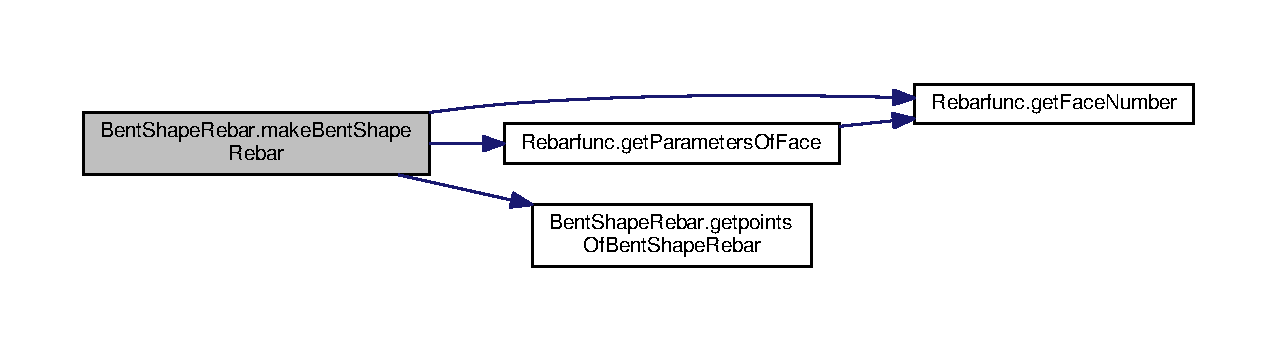
\includegraphics[width=350pt]{namespaceBentShapeRebar_aac46779d3e1905db5a3788917f6e2476_cgraph}
\end{center}
\end{figure}




Here is the caller graph for this function\+:\nopagebreak
\begin{figure}[H]
\begin{center}
\leavevmode
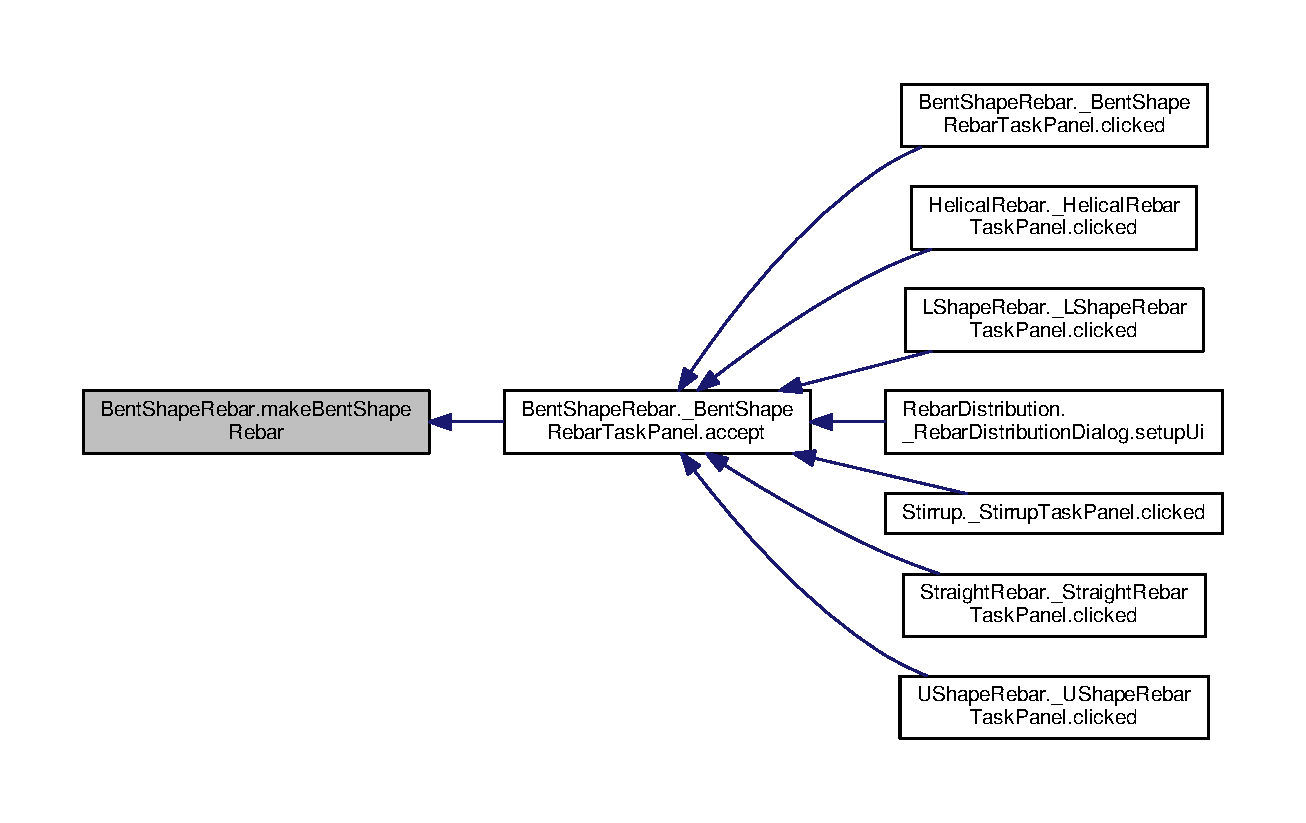
\includegraphics[width=350pt]{namespaceBentShapeRebar_aac46779d3e1905db5a3788917f6e2476_icgraph}
\end{center}
\end{figure}




\subsection{Variable Documentation}
\index{Bent\+Shape\+Rebar@{Bent\+Shape\+Rebar}!\+\_\+\+\_\+author\+\_\+\+\_\+@{\+\_\+\+\_\+author\+\_\+\+\_\+}}
\index{\+\_\+\+\_\+author\+\_\+\+\_\+@{\+\_\+\+\_\+author\+\_\+\+\_\+}!Bent\+Shape\+Rebar@{Bent\+Shape\+Rebar}}
\subsubsection[{\texorpdfstring{\+\_\+\+\_\+author\+\_\+\+\_\+}{__author__}}]{\setlength{\rightskip}{0pt plus 5cm}string Bent\+Shape\+Rebar.\+\_\+\+\_\+author\+\_\+\+\_\+ = \char`\"{}Amritpal Singh\char`\"{}\hspace{0.3cm}{\ttfamily [private]}}\hypertarget{namespaceBentShapeRebar_ad79a2dbf88601c24aae561033cb48d34}{}\label{namespaceBentShapeRebar_ad79a2dbf88601c24aae561033cb48d34}


Definition at line \hyperlink{BentShapeRebar_8py_source_l00025}{25} of file \hyperlink{BentShapeRebar_8py_source}{Bent\+Shape\+Rebar.\+py}.

\index{Bent\+Shape\+Rebar@{Bent\+Shape\+Rebar}!\+\_\+\+\_\+title\+\_\+\+\_\+@{\+\_\+\+\_\+title\+\_\+\+\_\+}}
\index{\+\_\+\+\_\+title\+\_\+\+\_\+@{\+\_\+\+\_\+title\+\_\+\+\_\+}!Bent\+Shape\+Rebar@{Bent\+Shape\+Rebar}}
\subsubsection[{\texorpdfstring{\+\_\+\+\_\+title\+\_\+\+\_\+}{__title__}}]{\setlength{\rightskip}{0pt plus 5cm}string Bent\+Shape\+Rebar.\+\_\+\+\_\+title\+\_\+\+\_\+ = \char`\"{}Bent\+Shape\+Rebar\char`\"{}\hspace{0.3cm}{\ttfamily [private]}}\hypertarget{namespaceBentShapeRebar_a38b223debc1826fd2855773a02749bb4}{}\label{namespaceBentShapeRebar_a38b223debc1826fd2855773a02749bb4}


Definition at line \hyperlink{BentShapeRebar_8py_source_l00024}{24} of file \hyperlink{BentShapeRebar_8py_source}{Bent\+Shape\+Rebar.\+py}.

\index{Bent\+Shape\+Rebar@{Bent\+Shape\+Rebar}!\+\_\+\+\_\+url\+\_\+\+\_\+@{\+\_\+\+\_\+url\+\_\+\+\_\+}}
\index{\+\_\+\+\_\+url\+\_\+\+\_\+@{\+\_\+\+\_\+url\+\_\+\+\_\+}!Bent\+Shape\+Rebar@{Bent\+Shape\+Rebar}}
\subsubsection[{\texorpdfstring{\+\_\+\+\_\+url\+\_\+\+\_\+}{__url__}}]{\setlength{\rightskip}{0pt plus 5cm}string Bent\+Shape\+Rebar.\+\_\+\+\_\+url\+\_\+\+\_\+ = \char`\"{}https\+://www.\+freecadweb.\+org\char`\"{}\hspace{0.3cm}{\ttfamily [private]}}\hypertarget{namespaceBentShapeRebar_aec768ca6a259d1cc738ea11c79a124e2}{}\label{namespaceBentShapeRebar_aec768ca6a259d1cc738ea11c79a124e2}


Definition at line \hyperlink{BentShapeRebar_8py_source_l00026}{26} of file \hyperlink{BentShapeRebar_8py_source}{Bent\+Shape\+Rebar.\+py}.


\hypertarget{namespaceHelicalRebar}{}\section{Helical\+Rebar Namespace Reference}
\label{namespaceHelicalRebar}\index{Helical\+Rebar@{Helical\+Rebar}}
\subsection*{Classes}
\begin{DoxyCompactItemize}
\item 
class \hyperlink{classHelicalRebar_1_1__HelicalRebarTaskPanel}{\+\_\+\+Helical\+Rebar\+Task\+Panel}
\end{DoxyCompactItemize}
\subsection*{Functions}
\begin{DoxyCompactItemize}
\item 
def \hyperlink{namespaceHelicalRebar_a4fcf2dabc065c39ce5c8cf6995051352}{getpoints\+Of\+Helical\+Rebar} (Face\+P\+RM, s\+\_\+cover, b\+\_\+cover, t\+\_\+cover, pitch, edges, diameter, size, direction)
\item 
def \hyperlink{namespaceHelicalRebar_a1a2b3ce39b904ab0c3892ed0965d2844}{create\+Helical\+Wire} (Face\+P\+RM, s\+\_\+cover, b\+\_\+cover, t\+\_\+cover, pitch, size, direction, helix=None)
\item 
def \hyperlink{namespaceHelicalRebar_a8a4f12ed70819996ac31877957dfab08}{make\+Helical\+Rebar} (s\+\_\+cover, b\+\_\+cover, diameter, t\+\_\+cover, pitch, structure=None, facename=None)
\item 
def \hyperlink{namespaceHelicalRebar_aea0d3838b1b171f801acf1046d111c8b}{edit\+Helical\+Rebar} (Rebar, s\+\_\+cover, b\+\_\+cover, diameter, t\+\_\+cover, pitch, structure=None, facename=None)
\item 
def \hyperlink{namespaceHelicalRebar_ab9725ab4f1e5650133dba94c24907331}{edit\+Dialog} (vobj)
\item 
def \hyperlink{namespaceHelicalRebar_ad8ff0caf1e8a56ac47ce25062db8bc46}{Command\+Helical\+Rebar} ()
\end{DoxyCompactItemize}
\subsection*{Variables}
\begin{DoxyCompactItemize}
\item 
string \hyperlink{namespaceHelicalRebar_a28c95505364eadd0c2d4abbd80091bef}{\+\_\+\+\_\+title\+\_\+\+\_\+} = \char`\"{}Helical\+Rebar\char`\"{}
\item 
string \hyperlink{namespaceHelicalRebar_a925dcfed2ffef215413157f48d7b6e57}{\+\_\+\+\_\+author\+\_\+\+\_\+} = \char`\"{}Amritpal Singh\char`\"{}
\item 
string \hyperlink{namespaceHelicalRebar_a9c74e4634d00eef07ed630054e69fbff}{\+\_\+\+\_\+url\+\_\+\+\_\+} = \char`\"{}https\+://www.\+freecadweb.\+org\char`\"{}
\end{DoxyCompactItemize}


\subsection{Function Documentation}
\index{Helical\+Rebar@{Helical\+Rebar}!Command\+Helical\+Rebar@{Command\+Helical\+Rebar}}
\index{Command\+Helical\+Rebar@{Command\+Helical\+Rebar}!Helical\+Rebar@{Helical\+Rebar}}
\subsubsection[{\texorpdfstring{Command\+Helical\+Rebar()}{CommandHelicalRebar()}}]{\setlength{\rightskip}{0pt plus 5cm}def Helical\+Rebar.\+Command\+Helical\+Rebar (
\begin{DoxyParamCaption}
{}
\end{DoxyParamCaption}
)}\hypertarget{namespaceHelicalRebar_ad8ff0caf1e8a56ac47ce25062db8bc46}{}\label{namespaceHelicalRebar_ad8ff0caf1e8a56ac47ce25062db8bc46}


Definition at line \hyperlink{HelicalRebar_8py_source_l00241}{241} of file \hyperlink{HelicalRebar_8py_source}{Helical\+Rebar.\+py}.


\begin{DoxyCode}
\hypertarget{namespaceHelicalRebar.tex_l00241}{}\hyperlink{namespaceHelicalRebar_ad8ff0caf1e8a56ac47ce25062db8bc46}{00241} \textcolor{keyword}{def }\hyperlink{namespaceHelicalRebar_ad8ff0caf1e8a56ac47ce25062db8bc46}{CommandHelicalRebar}():
00242     selected\_obj = \hyperlink{namespaceRebarfunc_adae2713855a7e1b4bda04081ae671542}{check\_selected\_face}()
00243     \textcolor{keywordflow}{if} selected\_obj:
00244         FreeCADGui.Control.showDialog(\hyperlink{classHelicalRebar_1_1__HelicalRebarTaskPanel}{\_HelicalRebarTaskPanel}())
00245 \end{DoxyCode}


Here is the call graph for this function\+:\nopagebreak
\begin{figure}[H]
\begin{center}
\leavevmode
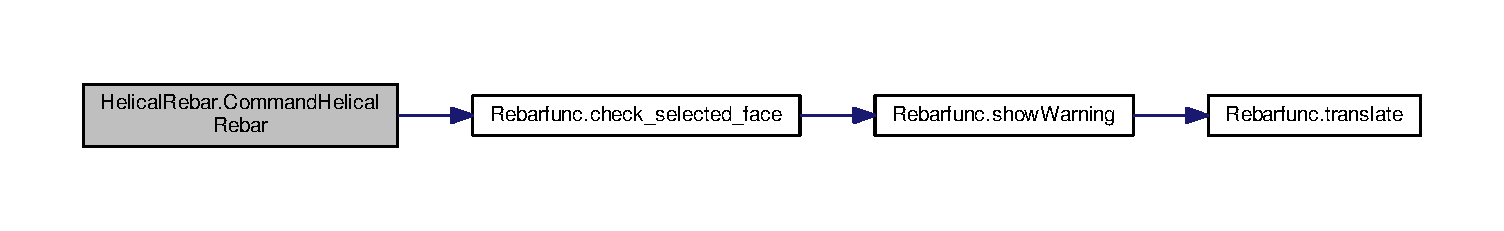
\includegraphics[width=350pt]{namespaceHelicalRebar_ad8ff0caf1e8a56ac47ce25062db8bc46_cgraph}
\end{center}
\end{figure}




Here is the caller graph for this function\+:\nopagebreak
\begin{figure}[H]
\begin{center}
\leavevmode
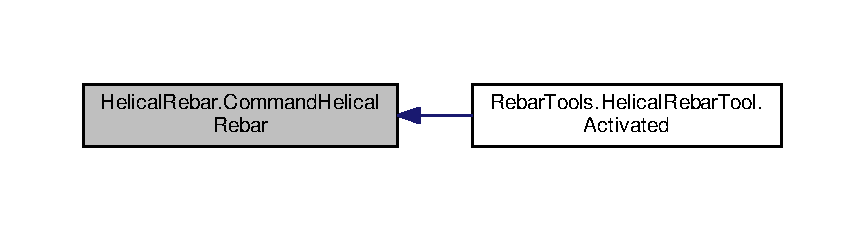
\includegraphics[width=350pt]{namespaceHelicalRebar_ad8ff0caf1e8a56ac47ce25062db8bc46_icgraph}
\end{center}
\end{figure}


\index{Helical\+Rebar@{Helical\+Rebar}!create\+Helical\+Wire@{create\+Helical\+Wire}}
\index{create\+Helical\+Wire@{create\+Helical\+Wire}!Helical\+Rebar@{Helical\+Rebar}}
\subsubsection[{\texorpdfstring{create\+Helical\+Wire(\+Face\+P\+R\+M, s\+\_\+cover, b\+\_\+cover, t\+\_\+cover, pitch, size, direction, helix=\+None)}{createHelicalWire(FacePRM, s_cover, b_cover, t_cover, pitch, size, direction, helix=None)}}]{\setlength{\rightskip}{0pt plus 5cm}def Helical\+Rebar.\+create\+Helical\+Wire (
\begin{DoxyParamCaption}
\item[{}]{Face\+P\+RM, }
\item[{}]{s\+\_\+cover, }
\item[{}]{b\+\_\+cover, }
\item[{}]{t\+\_\+cover, }
\item[{}]{pitch, }
\item[{}]{size, }
\item[{}]{direction, }
\item[{}]{helix = {\ttfamily None}}
\end{DoxyParamCaption}
)}\hypertarget{namespaceHelicalRebar_a1a2b3ce39b904ab0c3892ed0965d2844}{}\label{namespaceHelicalRebar_a1a2b3ce39b904ab0c3892ed0965d2844}
\begin{DoxyVerb}createHelicalWire(FacePRM, SideCover, BottomCover, TopCover, Pitch, Size, Direction, Helix = None):
It creates a helical wire.\end{DoxyVerb}
 

Definition at line \hyperlink{HelicalRebar_8py_source_l00075}{75} of file \hyperlink{HelicalRebar_8py_source}{Helical\+Rebar.\+py}.


\begin{DoxyCode}
\hypertarget{namespaceHelicalRebar.tex_l00075}{}\hyperlink{namespaceHelicalRebar_a1a2b3ce39b904ab0c3892ed0965d2844}{00075} \textcolor{keyword}{def }\hyperlink{namespaceHelicalRebar_a1a2b3ce39b904ab0c3892ed0965d2844}{createHelicalWire}(FacePRM, s\_cover, b\_cover, t\_cover, pitch, size, direction, helix = 
      None):
00076     \textcolor{stringliteral}{""" createHelicalWire(FacePRM, SideCover, BottomCover, TopCover, Pitch, Size, Direction, Helix = None):}
00077 \textcolor{stringliteral}{    It creates a helical wire."""}
00078     \textcolor{keyword}{import} Part
00079     \textcolor{keywordflow}{if} \textcolor{keywordflow}{not} helix:
00080         helix = FreeCAD.ActiveDocument.addObject(\textcolor{stringliteral}{"Part::Helix"},\textcolor{stringliteral}{"Helix"})
00081     helix.Pitch = pitch
00082     helix.Radius = FacePRM[0][0] / 2 - s\_cover
00083     helix.Angle = 0
00084     helix.LocalCoord = 0
00085     helix.Height = size - b\_cover - t\_cover
00086     \textcolor{keywordflow}{if} round(direction.x) == 1:
00087         helix.Placement.Base = FreeCAD.Vector(FacePRM[1][0] - b\_cover, FacePRM[1][1], FacePRM[1][2])
00088         helix.Placement.Rotation = FreeCAD.Rotation(FreeCAD.Vector(0, -1, 0), 90)
00089     \textcolor{keywordflow}{elif} round(direction.x) == -1:
00090         helix.Placement.Base = FreeCAD.Vector(FacePRM[1][0] + t\_cover, FacePRM[1][1], FacePRM[1][2])
00091         helix.Placement.Rotation = FreeCAD.Rotation(FreeCAD.Vector(0, -1, 0), -90)
00092     \textcolor{keywordflow}{elif} round(direction.y) == 1:
00093         helix.Placement.Base = FreeCAD.Vector(FacePRM[1][0], FacePRM[1][1] - b\_cover, FacePRM[1][2])
00094         helix.Placement.Rotation = FreeCAD.Rotation(FreeCAD.Vector(1, 0, 0), 90)
00095     \textcolor{keywordflow}{elif} round(direction.y) == -1:
00096         helix.Placement.Base = FreeCAD.Vector(FacePRM[1][0], FacePRM[1][1] + t\_cover, FacePRM[1][2])
00097         helix.Placement.Rotation = FreeCAD.Rotation(FreeCAD.Vector(-1, 0, 0), 90)
00098     \textcolor{keywordflow}{elif} round(direction.z) == 1:
00099         helix.Placement.Base = FreeCAD.Vector(FacePRM[1][0], FacePRM[1][1], FacePRM[1][2] - size + b\_cover)
00100         helix.Placement.Rotation = FreeCAD.Rotation(FreeCAD.Vector(0, 0, 1), 0)
00101     \textcolor{keywordflow}{elif} round(direction.z) == -1:
00102         helix.Placement.Base = FreeCAD.Vector(FacePRM[1][0], FacePRM[1][1], FacePRM[1][2] + b\_cover)
00103         helix.Placement.Rotation = FreeCAD.Rotation(FreeCAD.Vector(0, 0, -1), 0)
00104     FreeCAD.ActiveDocument.recompute()
00105     \textcolor{keywordflow}{return} helix
00106 
\end{DoxyCode}


Here is the caller graph for this function\+:\nopagebreak
\begin{figure}[H]
\begin{center}
\leavevmode
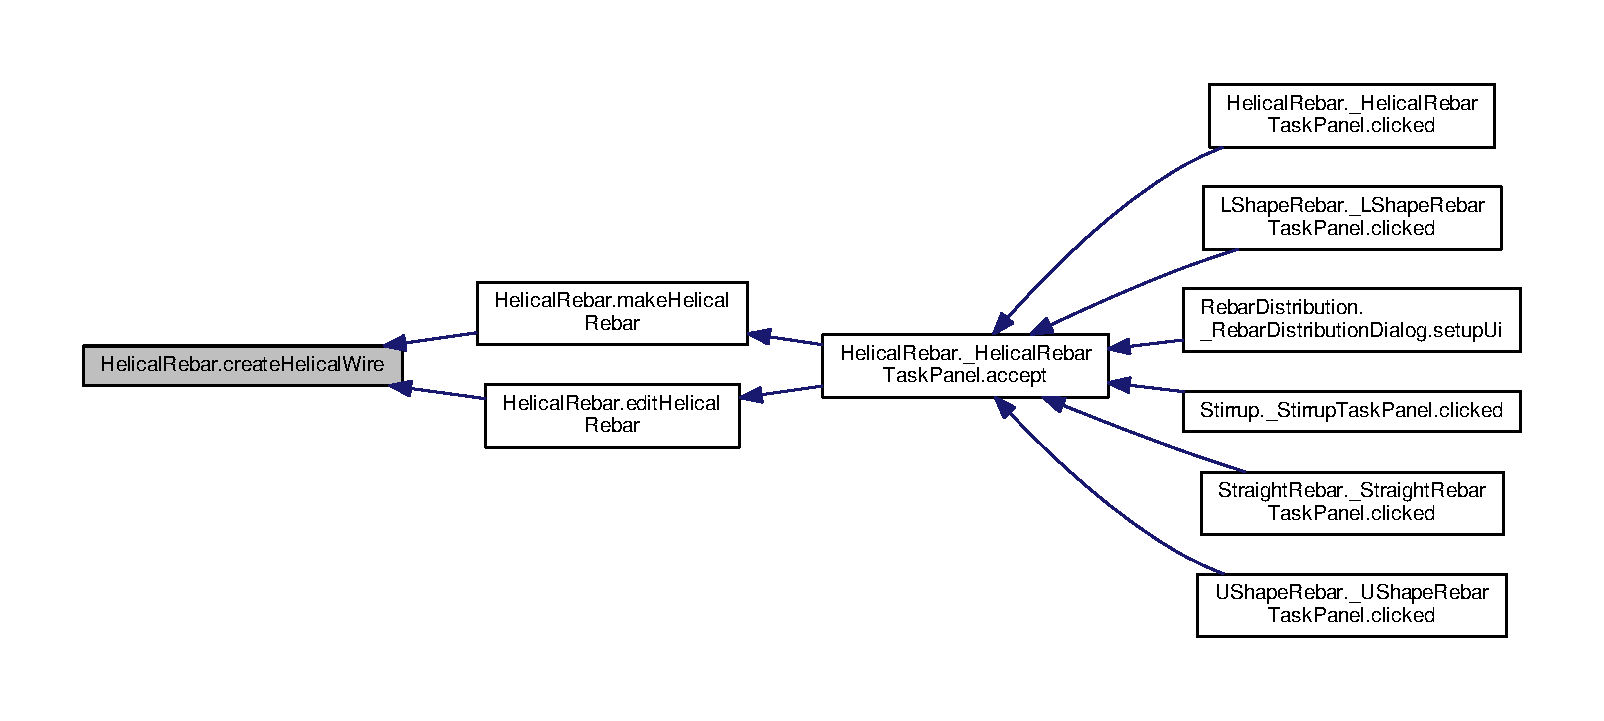
\includegraphics[width=350pt]{namespaceHelicalRebar_a1a2b3ce39b904ab0c3892ed0965d2844_icgraph}
\end{center}
\end{figure}


\index{Helical\+Rebar@{Helical\+Rebar}!edit\+Dialog@{edit\+Dialog}}
\index{edit\+Dialog@{edit\+Dialog}!Helical\+Rebar@{Helical\+Rebar}}
\subsubsection[{\texorpdfstring{edit\+Dialog(vobj)}{editDialog(vobj)}}]{\setlength{\rightskip}{0pt plus 5cm}def Helical\+Rebar.\+edit\+Dialog (
\begin{DoxyParamCaption}
\item[{}]{vobj}
\end{DoxyParamCaption}
)}\hypertarget{namespaceHelicalRebar_ab9725ab4f1e5650133dba94c24907331}{}\label{namespaceHelicalRebar_ab9725ab4f1e5650133dba94c24907331}


Definition at line \hyperlink{HelicalRebar_8py_source_l00231}{231} of file \hyperlink{HelicalRebar_8py_source}{Helical\+Rebar.\+py}.


\begin{DoxyCode}
\hypertarget{namespaceHelicalRebar.tex_l00231}{}\hyperlink{namespaceHelicalRebar_ab9725ab4f1e5650133dba94c24907331}{00231} \textcolor{keyword}{def }\hyperlink{namespaceHelicalRebar_ab9725ab4f1e5650133dba94c24907331}{editDialog}(vobj):
00232     FreeCADGui.Control.closeDialog()
00233     obj = \hyperlink{classHelicalRebar_1_1__HelicalRebarTaskPanel}{\_HelicalRebarTaskPanel}(vobj.Object)
00234     obj.form.sideCover.setText(str(vobj.Object.SideCover))
00235     obj.form.bottomCover.setText(str(vobj.Object.BottomCover))
00236     obj.form.diameter.setText(str(vobj.Object.Diameter))
00237     obj.form.topCover.setText(str(vobj.Object.TopCover))
00238     obj.form.pitch.setText(str(vobj.Object.Pitch))
00239     FreeCADGui.Control.showDialog(obj)
00240 
\end{DoxyCode}
\index{Helical\+Rebar@{Helical\+Rebar}!edit\+Helical\+Rebar@{edit\+Helical\+Rebar}}
\index{edit\+Helical\+Rebar@{edit\+Helical\+Rebar}!Helical\+Rebar@{Helical\+Rebar}}
\subsubsection[{\texorpdfstring{edit\+Helical\+Rebar(\+Rebar, s\+\_\+cover, b\+\_\+cover, diameter, t\+\_\+cover, pitch, structure=\+None, facename=\+None)}{editHelicalRebar(Rebar, s_cover, b_cover, diameter, t_cover, pitch, structure=None, facename=None)}}]{\setlength{\rightskip}{0pt plus 5cm}def Helical\+Rebar.\+edit\+Helical\+Rebar (
\begin{DoxyParamCaption}
\item[{}]{Rebar, }
\item[{}]{s\+\_\+cover, }
\item[{}]{b\+\_\+cover, }
\item[{}]{diameter, }
\item[{}]{t\+\_\+cover, }
\item[{}]{pitch, }
\item[{}]{structure = {\ttfamily None}, }
\item[{}]{facename = {\ttfamily None}}
\end{DoxyParamCaption}
)}\hypertarget{namespaceHelicalRebar_aea0d3838b1b171f801acf1046d111c8b}{}\label{namespaceHelicalRebar_aea0d3838b1b171f801acf1046d111c8b}


Definition at line \hyperlink{HelicalRebar_8py_source_l00203}{203} of file \hyperlink{HelicalRebar_8py_source}{Helical\+Rebar.\+py}.


\begin{DoxyCode}
\hypertarget{namespaceHelicalRebar.tex_l00203}{}\hyperlink{namespaceHelicalRebar_aea0d3838b1b171f801acf1046d111c8b}{00203} \textcolor{keyword}{def }\hyperlink{namespaceHelicalRebar_aea0d3838b1b171f801acf1046d111c8b}{editHelicalRebar}(Rebar, s\_cover, b\_cover, diameter, t\_cover, pitch, structure = None, 
      facename = None):
00204     sketch = Rebar.Base
00205     \textcolor{keywordflow}{if} structure \textcolor{keywordflow}{and} facename:
00206         sketch.Support = [(structure, facename)]
00207     \textcolor{comment}{# Check if sketch support is empty.}
00208     \textcolor{keywordflow}{if} \textcolor{keywordflow}{not} sketch.Support:
00209         \hyperlink{namespaceRebarfunc_a2278a0602d46a62953af1fcf2e574a94}{showWarning}(\textcolor{stringliteral}{"You have checked remove external geometry of base sketchs when needed.\(\backslash\)nTo
       unchecked Edit->Preferences->Arch."})
00210         \textcolor{keywordflow}{return}
00211     \textcolor{comment}{# Assigned values}
00212     facename = sketch.Support[0][1][0]
00213     structure = sketch.Support[0][0]
00214     face = structure.Shape.Faces[\hyperlink{namespaceRebarfunc_a3885b3b63e3a41508ac79bc7550cf301}{getFaceNumber}(facename) - 1]
00215     \textcolor{comment}{#StructurePRM = getTrueParametersOfStructure(structure)}
00216     \textcolor{comment}{# Get parameters of the face where sketch of rebar is drawn}
00217     FacePRM = \hyperlink{namespaceRebarfunc_a92122b3d7cedd3d47bb63380a5ac4d08}{getParametersOfFace}(structure, facename, \textcolor{keyword}{False})
00218     size = (ArchCommands.projectToVector(structure.Shape.copy(), face.normalAt(0, 0))).Length
00219     normal = face.normalAt(0,0)
00220     \textcolor{comment}{#normal = face.Placement.Rotation.inverted().multVec(normal)}
00221     helix = \hyperlink{namespaceHelicalRebar_a1a2b3ce39b904ab0c3892ed0965d2844}{createHelicalWire}(FacePRM, s\_cover, b\_cover, t\_cover, pitch, size, normal, 
      Rebar.Base)
00222     FreeCAD.ActiveDocument.recompute()
00223     Rebar.Diameter = diameter
00224     Rebar.SideCover = s\_cover
00225     Rebar.BottomCover = b\_cover
00226     Rebar.TopCover = t\_cover
00227     Rebar.Pitch = pitch
00228     FreeCAD.ActiveDocument.recompute()
00229     \textcolor{keywordflow}{return} Rebar
00230 
\end{DoxyCode}


Here is the call graph for this function\+:\nopagebreak
\begin{figure}[H]
\begin{center}
\leavevmode
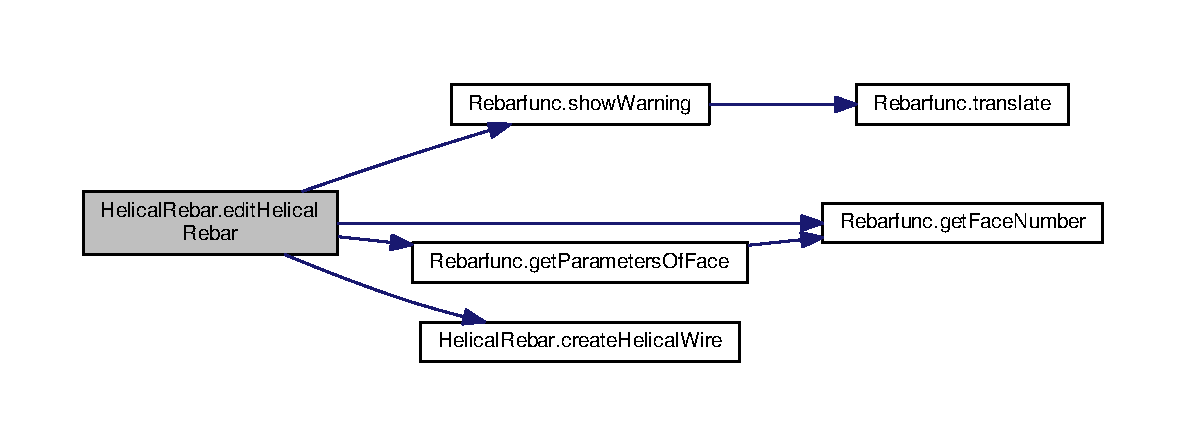
\includegraphics[width=350pt]{namespaceHelicalRebar_aea0d3838b1b171f801acf1046d111c8b_cgraph}
\end{center}
\end{figure}




Here is the caller graph for this function\+:\nopagebreak
\begin{figure}[H]
\begin{center}
\leavevmode
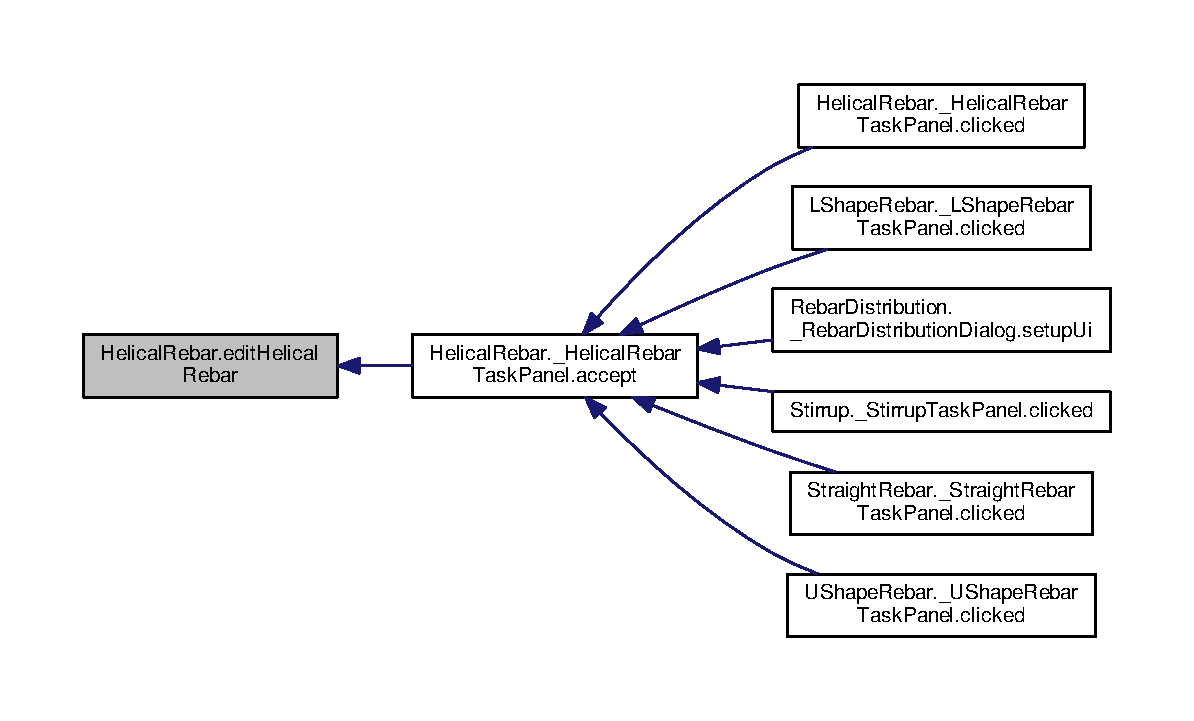
\includegraphics[width=350pt]{namespaceHelicalRebar_aea0d3838b1b171f801acf1046d111c8b_icgraph}
\end{center}
\end{figure}


\index{Helical\+Rebar@{Helical\+Rebar}!getpoints\+Of\+Helical\+Rebar@{getpoints\+Of\+Helical\+Rebar}}
\index{getpoints\+Of\+Helical\+Rebar@{getpoints\+Of\+Helical\+Rebar}!Helical\+Rebar@{Helical\+Rebar}}
\subsubsection[{\texorpdfstring{getpoints\+Of\+Helical\+Rebar(\+Face\+P\+R\+M, s\+\_\+cover, b\+\_\+cover, t\+\_\+cover, pitch, edges, diameter, size, direction)}{getpointsOfHelicalRebar(FacePRM, s_cover, b_cover, t_cover, pitch, edges, diameter, size, direction)}}]{\setlength{\rightskip}{0pt plus 5cm}def Helical\+Rebar.\+getpoints\+Of\+Helical\+Rebar (
\begin{DoxyParamCaption}
\item[{}]{Face\+P\+RM, }
\item[{}]{s\+\_\+cover, }
\item[{}]{b\+\_\+cover, }
\item[{}]{t\+\_\+cover, }
\item[{}]{pitch, }
\item[{}]{edges, }
\item[{}]{diameter, }
\item[{}]{size, }
\item[{}]{direction}
\end{DoxyParamCaption}
)}\hypertarget{namespaceHelicalRebar_a4fcf2dabc065c39ce5c8cf6995051352}{}\label{namespaceHelicalRebar_a4fcf2dabc065c39ce5c8cf6995051352}
\begin{DoxyVerb}getpointsOfHelicalRebar(FacePRM, s_cover, b_cover, t_cover):
Return points of the LShape rebar in the form of array for sketch.\end{DoxyVerb}
 

Definition at line \hyperlink{HelicalRebar_8py_source_l00039}{39} of file \hyperlink{HelicalRebar_8py_source}{Helical\+Rebar.\+py}.


\begin{DoxyCode}
\hypertarget{namespaceHelicalRebar.tex_l00039}{}\hyperlink{namespaceHelicalRebar_a4fcf2dabc065c39ce5c8cf6995051352}{00039} \textcolor{keyword}{def }\hyperlink{namespaceHelicalRebar_a4fcf2dabc065c39ce5c8cf6995051352}{getpointsOfHelicalRebar}(FacePRM, s\_cover, b\_cover, t\_cover, pitch, edges, 
      diameter, size, direction):
00040     \textcolor{stringliteral}{""" getpointsOfHelicalRebar(FacePRM, s\_cover, b\_cover, t\_cover):}
00041 \textcolor{stringliteral}{    Return points of the LShape rebar in the form of array for sketch."""}
00042     dx = s\_cover + diameter / 2
00043     dz = float(pitch) / edges
00044     R = diameter / 2 - dx
00045     R = FacePRM[0][0] / 2 - s\_cover
00046     points = []
00047     \textcolor{keywordflow}{if} direction[2] \textcolor{keywordflow}{in} \{-1,1\}:
00048         z = 0
00049         l = 0
00050         \textcolor{keywordflow}{if} direction[2] == 1:
00051             zz = FacePRM[1][2] - t\_cover
00052         \textcolor{keywordflow}{elif} direction[2] == -1:
00053             zz = FacePRM[1][2] + b\_cover
00054         count = 0
00055         flag = \textcolor{keyword}{False}
00056         \textcolor{keywordflow}{while} (round(z) < abs(size - b\_cover - t\_cover)):
00057             \textcolor{keywordflow}{for} i \textcolor{keywordflow}{in} range(0, int(edges) + 1):
00058                 \textcolor{keywordflow}{if} \textcolor{keywordflow}{not} i \textcolor{keywordflow}{and} flag:
00059                     \textcolor{keywordflow}{continue}
00060                 \textcolor{keywordflow}{if} \textcolor{keywordflow}{not} flag:
00061                     z -= dz
00062                     flag = \textcolor{keyword}{True}
00063                 iAngle = i * 360 / edges
00064                 x =  FacePRM[1][0] + R * math.cos(math.radians(iAngle))
00065                 y =  FacePRM[1][1] + R * math.sin(math.radians(iAngle))
00066                 points.append(FreeCAD.Vector(x, y, zz))
00067                 count += 1
00068                 \textcolor{keywordflow}{if} direction[2] == 1:
00069                     zz -= dz
00070                 \textcolor{keywordflow}{elif} direction[2] == -1:
00071                     zz += dz
00072                 z += dz
00073     \textcolor{keywordflow}{return} points
00074 
\end{DoxyCode}
\index{Helical\+Rebar@{Helical\+Rebar}!make\+Helical\+Rebar@{make\+Helical\+Rebar}}
\index{make\+Helical\+Rebar@{make\+Helical\+Rebar}!Helical\+Rebar@{Helical\+Rebar}}
\subsubsection[{\texorpdfstring{make\+Helical\+Rebar(s\+\_\+cover, b\+\_\+cover, diameter, t\+\_\+cover, pitch, structure=\+None, facename=\+None)}{makeHelicalRebar(s_cover, b_cover, diameter, t_cover, pitch, structure=None, facename=None)}}]{\setlength{\rightskip}{0pt plus 5cm}def Helical\+Rebar.\+make\+Helical\+Rebar (
\begin{DoxyParamCaption}
\item[{}]{s\+\_\+cover, }
\item[{}]{b\+\_\+cover, }
\item[{}]{diameter, }
\item[{}]{t\+\_\+cover, }
\item[{}]{pitch, }
\item[{}]{structure = {\ttfamily None}, }
\item[{}]{facename = {\ttfamily None}}
\end{DoxyParamCaption}
)}\hypertarget{namespaceHelicalRebar_a8a4f12ed70819996ac31877957dfab08}{}\label{namespaceHelicalRebar_a8a4f12ed70819996ac31877957dfab08}
\begin{DoxyVerb}makeHelicalRebar(SideCover, BottomCover, Diameter, TopCover, Pitch, Structure, Facename):
Adds the Helical reinforcement bar to the selected structural object.\end{DoxyVerb}
 

Definition at line \hyperlink{HelicalRebar_8py_source_l00165}{165} of file \hyperlink{HelicalRebar_8py_source}{Helical\+Rebar.\+py}.


\begin{DoxyCode}
\hypertarget{namespaceHelicalRebar.tex_l00165}{}\hyperlink{namespaceHelicalRebar_a8a4f12ed70819996ac31877957dfab08}{00165} \textcolor{keyword}{def }\hyperlink{namespaceHelicalRebar_a8a4f12ed70819996ac31877957dfab08}{makeHelicalRebar}(s\_cover, b\_cover, diameter, t\_cover, pitch, structure = None, facename
       = None):
00166     \textcolor{stringliteral}{""" makeHelicalRebar(SideCover, BottomCover, Diameter, TopCover, Pitch, Structure, Facename):}
00167 \textcolor{stringliteral}{    Adds the Helical reinforcement bar to the selected structural object."""}
00168     \textcolor{keywordflow}{if} \textcolor{keywordflow}{not} structure \textcolor{keywordflow}{and} \textcolor{keywordflow}{not} facename:
00169         selected\_obj = FreeCADGui.Selection.getSelectionEx()[0]
00170         structure = selected\_obj.Object
00171         facename = selected\_obj.SubElementNames[0]
00172     face = structure.Shape.Faces[\hyperlink{namespaceRebarfunc_a3885b3b63e3a41508ac79bc7550cf301}{getFaceNumber}(facename) - 1]
00173     \textcolor{comment}{#StructurePRM = getTrueParametersOfStructure(structure)}
00174     FacePRM = \hyperlink{namespaceRebarfunc_a92122b3d7cedd3d47bb63380a5ac4d08}{getParametersOfFace}(structure, facename, \textcolor{keyword}{False})
00175     \textcolor{keywordflow}{if} \textcolor{keywordflow}{not} FacePRM:
00176         FreeCAD.Console.PrintError(\textcolor{stringliteral}{"Cannot identified shape or from which base object sturctural element is
       derived\(\backslash\)n"})
00177         \textcolor{keywordflow}{return}
00178     size = (ArchCommands.projectToVector(structure.Shape.copy(), face.normalAt(0, 0))).Length
00179     normal = face.normalAt(0,0)
00180     \textcolor{comment}{#normal = face.Placement.Rotation.inverted().multVec(normal)}
00181     \textcolor{keyword}{import} Arch
00182     helix = \hyperlink{namespaceHelicalRebar_a1a2b3ce39b904ab0c3892ed0965d2844}{createHelicalWire}(FacePRM, s\_cover, b\_cover, t\_cover, pitch, size, normal)
00183     helix.Support = [(structure, facename)]
00184     rebar = Arch.makeRebar(structure, helix, diameter, 1, 0)
00185     rebar.OffsetStart = 0
00186     rebar.OffsetEnd = 0
00187     FreeCAD.ActiveDocument.recompute()
00188     \textcolor{comment}{# Adds properties to the rebar object}
00189     rebar.ViewObject.addProperty(\textcolor{stringliteral}{"App::PropertyString"}, \textcolor{stringliteral}{"RebarShape"}, \textcolor{stringliteral}{"RebarDialog"}, QT\_TRANSLATE\_NOOP(\textcolor{stringliteral}{"
      App::Property"}, \textcolor{stringliteral}{"Shape of rebar"})).RebarShape = \textcolor{stringliteral}{"HelicalRebar"}
00190     rebar.ViewObject.setEditorMode(\textcolor{stringliteral}{"RebarShape"}, 2)
00191     rebar.addProperty(\textcolor{stringliteral}{"App::PropertyDistance"}, \textcolor{stringliteral}{"SideCover"}, \textcolor{stringliteral}{"RebarDialog"}, QT\_TRANSLATE\_NOOP(\textcolor{stringliteral}{"App::Property
      "}, \textcolor{stringliteral}{"Front cover of rebar"})).SideCover = s\_cover
00192     rebar.setEditorMode(\textcolor{stringliteral}{"SideCover"}, 2)
00193     rebar.addProperty(\textcolor{stringliteral}{"App::PropertyDistance"}, \textcolor{stringliteral}{"Pitch"}, \textcolor{stringliteral}{"RebarDialog"}, QT\_TRANSLATE\_NOOP(\textcolor{stringliteral}{"App::Property"}, \textcolor{stringliteral}{"
      Left Side cover of rebar"})).Pitch = pitch
00194     rebar.setEditorMode(\textcolor{stringliteral}{"Pitch"}, 2)
00195     rebar.addProperty(\textcolor{stringliteral}{"App::PropertyDistance"}, \textcolor{stringliteral}{"BottomCover"}, \textcolor{stringliteral}{"RebarDialog"}, QT\_TRANSLATE\_NOOP(\textcolor{stringliteral}{"
      App::Property"}, \textcolor{stringliteral}{"Bottom cover of rebar"})).BottomCover = b\_cover
00196     rebar.setEditorMode(\textcolor{stringliteral}{"BottomCover"}, 2)
00197     rebar.addProperty(\textcolor{stringliteral}{"App::PropertyDistance"}, \textcolor{stringliteral}{"TopCover"}, \textcolor{stringliteral}{"RebarDialog"}, QT\_TRANSLATE\_NOOP(\textcolor{stringliteral}{"App::Property"}
      , \textcolor{stringliteral}{"Top cover of rebar"})).TopCover = t\_cover
00198     rebar.setEditorMode(\textcolor{stringliteral}{"TopCover"}, 2)
00199     rebar.Label = \textcolor{stringliteral}{"HelicalRebar"}
00200     FreeCAD.ActiveDocument.recompute()
00201     \textcolor{keywordflow}{return} rebar
00202 
\end{DoxyCode}


Here is the call graph for this function\+:\nopagebreak
\begin{figure}[H]
\begin{center}
\leavevmode
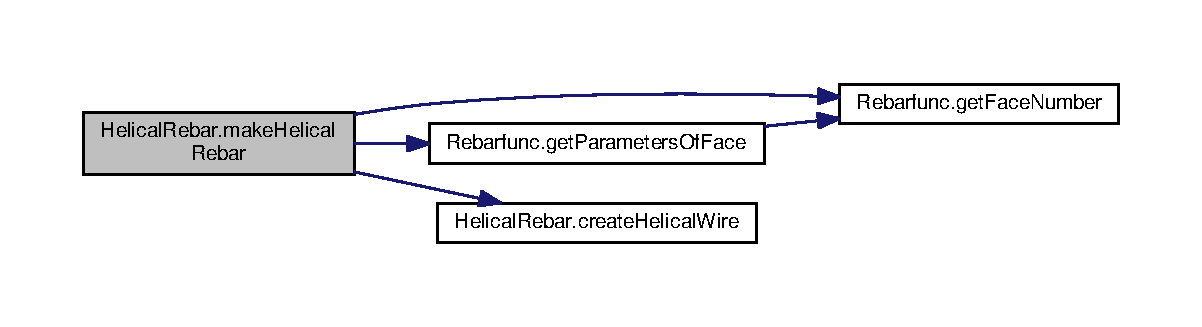
\includegraphics[width=350pt]{namespaceHelicalRebar_a8a4f12ed70819996ac31877957dfab08_cgraph}
\end{center}
\end{figure}




Here is the caller graph for this function\+:\nopagebreak
\begin{figure}[H]
\begin{center}
\leavevmode
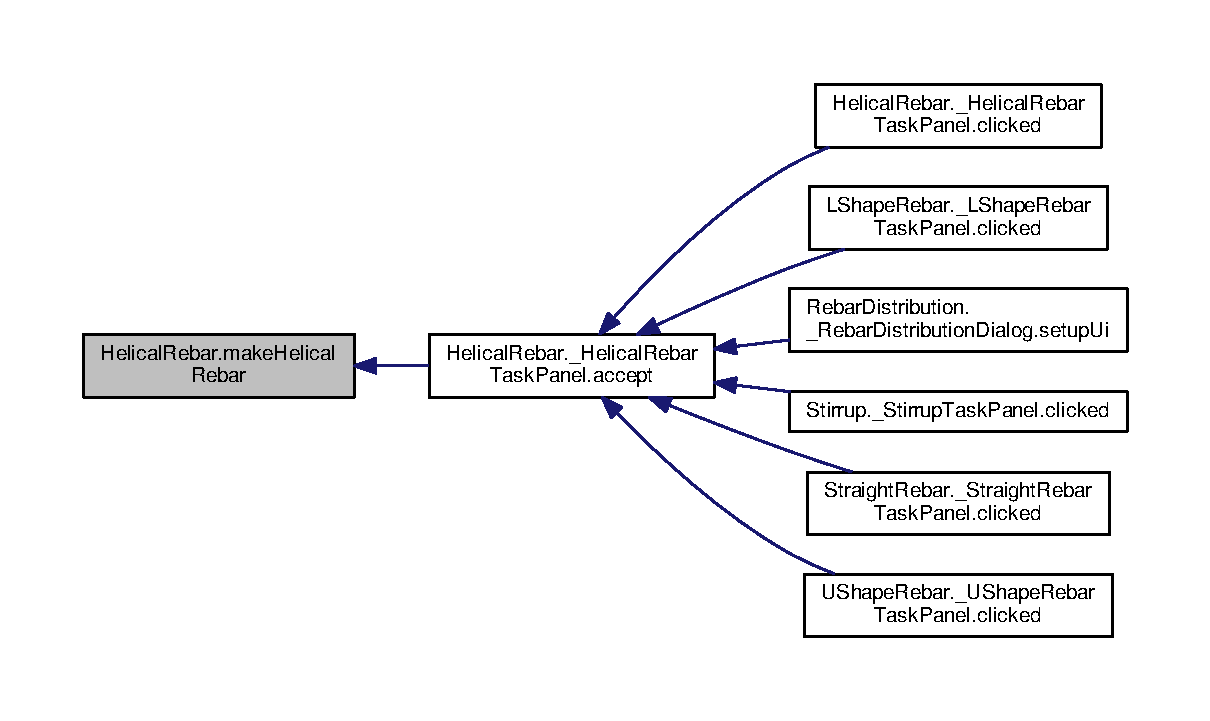
\includegraphics[width=350pt]{namespaceHelicalRebar_a8a4f12ed70819996ac31877957dfab08_icgraph}
\end{center}
\end{figure}




\subsection{Variable Documentation}
\index{Helical\+Rebar@{Helical\+Rebar}!\+\_\+\+\_\+author\+\_\+\+\_\+@{\+\_\+\+\_\+author\+\_\+\+\_\+}}
\index{\+\_\+\+\_\+author\+\_\+\+\_\+@{\+\_\+\+\_\+author\+\_\+\+\_\+}!Helical\+Rebar@{Helical\+Rebar}}
\subsubsection[{\texorpdfstring{\+\_\+\+\_\+author\+\_\+\+\_\+}{__author__}}]{\setlength{\rightskip}{0pt plus 5cm}string Helical\+Rebar.\+\_\+\+\_\+author\+\_\+\+\_\+ = \char`\"{}Amritpal Singh\char`\"{}\hspace{0.3cm}{\ttfamily [private]}}\hypertarget{namespaceHelicalRebar_a925dcfed2ffef215413157f48d7b6e57}{}\label{namespaceHelicalRebar_a925dcfed2ffef215413157f48d7b6e57}


Definition at line \hyperlink{HelicalRebar_8py_source_l00025}{25} of file \hyperlink{HelicalRebar_8py_source}{Helical\+Rebar.\+py}.

\index{Helical\+Rebar@{Helical\+Rebar}!\+\_\+\+\_\+title\+\_\+\+\_\+@{\+\_\+\+\_\+title\+\_\+\+\_\+}}
\index{\+\_\+\+\_\+title\+\_\+\+\_\+@{\+\_\+\+\_\+title\+\_\+\+\_\+}!Helical\+Rebar@{Helical\+Rebar}}
\subsubsection[{\texorpdfstring{\+\_\+\+\_\+title\+\_\+\+\_\+}{__title__}}]{\setlength{\rightskip}{0pt plus 5cm}string Helical\+Rebar.\+\_\+\+\_\+title\+\_\+\+\_\+ = \char`\"{}Helical\+Rebar\char`\"{}\hspace{0.3cm}{\ttfamily [private]}}\hypertarget{namespaceHelicalRebar_a28c95505364eadd0c2d4abbd80091bef}{}\label{namespaceHelicalRebar_a28c95505364eadd0c2d4abbd80091bef}


Definition at line \hyperlink{HelicalRebar_8py_source_l00024}{24} of file \hyperlink{HelicalRebar_8py_source}{Helical\+Rebar.\+py}.

\index{Helical\+Rebar@{Helical\+Rebar}!\+\_\+\+\_\+url\+\_\+\+\_\+@{\+\_\+\+\_\+url\+\_\+\+\_\+}}
\index{\+\_\+\+\_\+url\+\_\+\+\_\+@{\+\_\+\+\_\+url\+\_\+\+\_\+}!Helical\+Rebar@{Helical\+Rebar}}
\subsubsection[{\texorpdfstring{\+\_\+\+\_\+url\+\_\+\+\_\+}{__url__}}]{\setlength{\rightskip}{0pt plus 5cm}string Helical\+Rebar.\+\_\+\+\_\+url\+\_\+\+\_\+ = \char`\"{}https\+://www.\+freecadweb.\+org\char`\"{}\hspace{0.3cm}{\ttfamily [private]}}\hypertarget{namespaceHelicalRebar_a9c74e4634d00eef07ed630054e69fbff}{}\label{namespaceHelicalRebar_a9c74e4634d00eef07ed630054e69fbff}


Definition at line \hyperlink{HelicalRebar_8py_source_l00026}{26} of file \hyperlink{HelicalRebar_8py_source}{Helical\+Rebar.\+py}.


\hypertarget{namespaceLShapeRebar}{}\section{L\+Shape\+Rebar Namespace Reference}
\label{namespaceLShapeRebar}\index{L\+Shape\+Rebar@{L\+Shape\+Rebar}}
\subsection*{Classes}
\begin{DoxyCompactItemize}
\item 
class \hyperlink{classLShapeRebar_1_1__LShapeRebarTaskPanel}{\+\_\+\+L\+Shape\+Rebar\+Task\+Panel}
\end{DoxyCompactItemize}
\subsection*{Functions}
\begin{DoxyCompactItemize}
\item 
def \hyperlink{namespaceLShapeRebar_a3019960c6f6476cb70df9ee06f330dfb}{getpoints\+Of\+L\+Shape\+Rebar} (Face\+P\+RM, l\+\_\+cover, r\+\_\+cover, b\+\_\+cover, t\+\_\+cover, orientation)
\item 
def \hyperlink{namespaceLShapeRebar_a647a28e94933108c6617da8532d76998}{make\+L\+Shape\+Rebar} (f\+\_\+cover, b\+\_\+cover, l\+\_\+cover, r\+\_\+cover, diameter, t\+\_\+cover, rounding, amount\+\_\+spacing\+\_\+check, amount\+\_\+spacing\+\_\+value, orientation=\char`\"{}Bottom Left\char`\"{}, structure=None, facename=None)
\item 
def \hyperlink{namespaceLShapeRebar_a9915291e3457e1c27f556d7903e02486}{edit\+L\+Shape\+Rebar} (Rebar, f\+\_\+cover, b\+\_\+cover, l\+\_\+cover, r\+\_\+cover, diameter, t\+\_\+cover, rounding, amount\+\_\+spacing\+\_\+check, amount\+\_\+spacing\+\_\+value, orientation, structure=None, facename=None)
\item 
def \hyperlink{namespaceLShapeRebar_a73f1b8d577fecf230a8c071424b2015e}{edit\+Dialog} (vobj)
\item 
def \hyperlink{namespaceLShapeRebar_a5439b0c3265fa6d432d4a81e47f4441e}{Command\+L\+Shape\+Rebar} ()
\end{DoxyCompactItemize}
\subsection*{Variables}
\begin{DoxyCompactItemize}
\item 
string \hyperlink{namespaceLShapeRebar_a0ac8e9cb97e560c6ce362c1ac5144c31}{\+\_\+\+\_\+title\+\_\+\+\_\+} = \char`\"{}L\+Shape\+Rebar\char`\"{}
\item 
string \hyperlink{namespaceLShapeRebar_ad398517c2df8a455dfd0b670e54285ea}{\+\_\+\+\_\+author\+\_\+\+\_\+} = \char`\"{}Amritpal Singh\char`\"{}
\item 
string \hyperlink{namespaceLShapeRebar_a7bca929f0dda68928d1f3978b4e877f8}{\+\_\+\+\_\+url\+\_\+\+\_\+} = \char`\"{}https\+://www.\+freecadweb.\+org\char`\"{}
\end{DoxyCompactItemize}


\subsection{Function Documentation}
\index{L\+Shape\+Rebar@{L\+Shape\+Rebar}!Command\+L\+Shape\+Rebar@{Command\+L\+Shape\+Rebar}}
\index{Command\+L\+Shape\+Rebar@{Command\+L\+Shape\+Rebar}!L\+Shape\+Rebar@{L\+Shape\+Rebar}}
\subsubsection[{\texorpdfstring{Command\+L\+Shape\+Rebar()}{CommandLShapeRebar()}}]{\setlength{\rightskip}{0pt plus 5cm}def L\+Shape\+Rebar.\+Command\+L\+Shape\+Rebar (
\begin{DoxyParamCaption}
{}
\end{DoxyParamCaption}
)}\hypertarget{namespaceLShapeRebar_a5439b0c3265fa6d432d4a81e47f4441e}{}\label{namespaceLShapeRebar_a5439b0c3265fa6d432d4a81e47f4441e}


Definition at line \hyperlink{LShapeRebar_8py_source_l00300}{300} of file \hyperlink{LShapeRebar_8py_source}{L\+Shape\+Rebar.\+py}.


\begin{DoxyCode}
\hypertarget{namespaceLShapeRebar.tex_l00300}{}\hyperlink{namespaceLShapeRebar_a5439b0c3265fa6d432d4a81e47f4441e}{00300} \textcolor{keyword}{def }\hyperlink{namespaceLShapeRebar_a5439b0c3265fa6d432d4a81e47f4441e}{CommandLShapeRebar}():
00301     selected\_obj = \hyperlink{namespaceRebarfunc_adae2713855a7e1b4bda04081ae671542}{check\_selected\_face}()
00302     \textcolor{keywordflow}{if} selected\_obj:
00303         FreeCADGui.Control.showDialog(\hyperlink{classLShapeRebar_1_1__LShapeRebarTaskPanel}{\_LShapeRebarTaskPanel}())
00304 \end{DoxyCode}


Here is the call graph for this function\+:\nopagebreak
\begin{figure}[H]
\begin{center}
\leavevmode
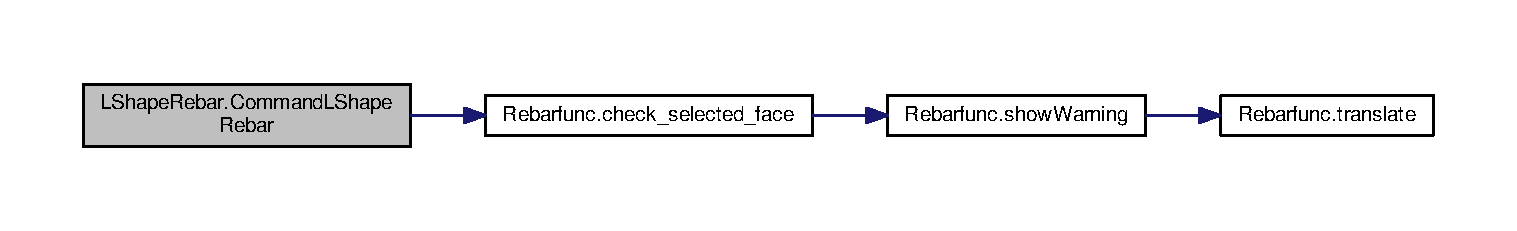
\includegraphics[width=350pt]{namespaceLShapeRebar_a5439b0c3265fa6d432d4a81e47f4441e_cgraph}
\end{center}
\end{figure}




Here is the caller graph for this function\+:\nopagebreak
\begin{figure}[H]
\begin{center}
\leavevmode
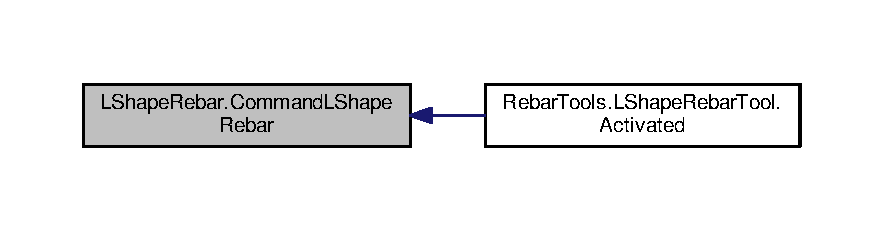
\includegraphics[width=350pt]{namespaceLShapeRebar_a5439b0c3265fa6d432d4a81e47f4441e_icgraph}
\end{center}
\end{figure}


\index{L\+Shape\+Rebar@{L\+Shape\+Rebar}!edit\+Dialog@{edit\+Dialog}}
\index{edit\+Dialog@{edit\+Dialog}!L\+Shape\+Rebar@{L\+Shape\+Rebar}}
\subsubsection[{\texorpdfstring{edit\+Dialog(vobj)}{editDialog(vobj)}}]{\setlength{\rightskip}{0pt plus 5cm}def L\+Shape\+Rebar.\+edit\+Dialog (
\begin{DoxyParamCaption}
\item[{}]{vobj}
\end{DoxyParamCaption}
)}\hypertarget{namespaceLShapeRebar_a73f1b8d577fecf230a8c071424b2015e}{}\label{namespaceLShapeRebar_a73f1b8d577fecf230a8c071424b2015e}


Definition at line \hyperlink{LShapeRebar_8py_source_l00278}{278} of file \hyperlink{LShapeRebar_8py_source}{L\+Shape\+Rebar.\+py}.


\begin{DoxyCode}
\hypertarget{namespaceLShapeRebar.tex_l00278}{}\hyperlink{namespaceLShapeRebar_a73f1b8d577fecf230a8c071424b2015e}{00278} \textcolor{keyword}{def }\hyperlink{namespaceLShapeRebar_a73f1b8d577fecf230a8c071424b2015e}{editDialog}(vobj):
00279     FreeCADGui.Control.closeDialog()
00280     obj = \hyperlink{classLShapeRebar_1_1__LShapeRebarTaskPanel}{\_LShapeRebarTaskPanel}(vobj.Object)
00281     obj.form.frontCover.setText(str(vobj.Object.FrontCover))
00282     obj.form.l\_sideCover.setText(str(vobj.Object.LeftCover))
00283     obj.form.r\_sideCover.setText(str(vobj.Object.RightCover))
00284     obj.form.bottomCover.setText(str(vobj.Object.BottomCover))
00285     obj.form.diameter.setText(str(vobj.Object.Diameter))
00286     obj.form.topCover.setText(str(vobj.Object.TopCover))
00287     obj.form.rounding.setValue(vobj.Object.Rounding)
00288     obj.form.orientation.setCurrentIndex(obj.form.orientation.findText(str(vobj.Object.Orientation)))
00289     \textcolor{keywordflow}{if} vobj.Object.AmountCheck:
00290         obj.form.amount.setValue(vobj.Object.Amount)
00291     \textcolor{keywordflow}{else}:
00292         obj.form.amount\_radio.setChecked(\textcolor{keyword}{False})
00293         obj.form.spacing\_radio.setChecked(\textcolor{keyword}{True})
00294         obj.form.amount.setDisabled(\textcolor{keyword}{True})
00295         obj.form.spacing.setEnabled(\textcolor{keyword}{True})
00296         obj.form.spacing.setText(str(vobj.Object.TrueSpacing))
00297     \textcolor{comment}{#obj.form.PickSelectedFace.setVisible(False)}
00298     FreeCADGui.Control.showDialog(obj)
00299 
\end{DoxyCode}
\index{L\+Shape\+Rebar@{L\+Shape\+Rebar}!edit\+L\+Shape\+Rebar@{edit\+L\+Shape\+Rebar}}
\index{edit\+L\+Shape\+Rebar@{edit\+L\+Shape\+Rebar}!L\+Shape\+Rebar@{L\+Shape\+Rebar}}
\subsubsection[{\texorpdfstring{edit\+L\+Shape\+Rebar(\+Rebar, f\+\_\+cover, b\+\_\+cover, l\+\_\+cover, r\+\_\+cover, diameter, t\+\_\+cover, rounding, amount\+\_\+spacing\+\_\+check, amount\+\_\+spacing\+\_\+value, orientation, structure=\+None, facename=\+None)}{editLShapeRebar(Rebar, f_cover, b_cover, l_cover, r_cover, diameter, t_cover, rounding, amount_spacing_check, amount_spacing_value, orientation, structure=None, facename=None)}}]{\setlength{\rightskip}{0pt plus 5cm}def L\+Shape\+Rebar.\+edit\+L\+Shape\+Rebar (
\begin{DoxyParamCaption}
\item[{}]{Rebar, }
\item[{}]{f\+\_\+cover, }
\item[{}]{b\+\_\+cover, }
\item[{}]{l\+\_\+cover, }
\item[{}]{r\+\_\+cover, }
\item[{}]{diameter, }
\item[{}]{t\+\_\+cover, }
\item[{}]{rounding, }
\item[{}]{amount\+\_\+spacing\+\_\+check, }
\item[{}]{amount\+\_\+spacing\+\_\+value, }
\item[{}]{orientation, }
\item[{}]{structure = {\ttfamily None}, }
\item[{}]{facename = {\ttfamily None}}
\end{DoxyParamCaption}
)}\hypertarget{namespaceLShapeRebar_a9915291e3457e1c27f556d7903e02486}{}\label{namespaceLShapeRebar_a9915291e3457e1c27f556d7903e02486}


Definition at line \hyperlink{LShapeRebar_8py_source_l00230}{230} of file \hyperlink{LShapeRebar_8py_source}{L\+Shape\+Rebar.\+py}.


\begin{DoxyCode}
\hypertarget{namespaceLShapeRebar.tex_l00230}{}\hyperlink{namespaceLShapeRebar_a9915291e3457e1c27f556d7903e02486}{00230} \textcolor{keyword}{def }\hyperlink{namespaceLShapeRebar_a9915291e3457e1c27f556d7903e02486}{editLShapeRebar}(Rebar, f\_cover, b\_cover, l\_cover, r\_cover, diameter, t\_cover, rounding, 
      amount\_spacing\_check, amount\_spacing\_value, orientation, structure = None, facename = None):
00231     sketch = Rebar.Base
00232     \textcolor{keywordflow}{if} structure \textcolor{keywordflow}{and} facename:
00233         sketch.Support = [(structure, facename)]
00234     \textcolor{comment}{# Check if sketch support is empty.}
00235     \textcolor{keywordflow}{if} \textcolor{keywordflow}{not} sketch.Support:
00236         \hyperlink{namespaceRebarfunc_a2278a0602d46a62953af1fcf2e574a94}{showWarning}(\textcolor{stringliteral}{"You have checked remove external geometry of base sketchs when needed.\(\backslash\)nTo
       unchecked Edit->Preferences->Arch."})
00237         \textcolor{keywordflow}{return}
00238     \textcolor{comment}{# Assigned values}
00239     facename = sketch.Support[0][1][0]
00240     structure = sketch.Support[0][0]
00241     face = structure.Shape.Faces[\hyperlink{namespaceRebarfunc_a3885b3b63e3a41508ac79bc7550cf301}{getFaceNumber}(facename) - 1]
00242     \textcolor{comment}{#StructurePRM = getTrueParametersOfStructure(structure)}
00243     \textcolor{comment}{# Get parameters of the face where sketch of rebar is drawn}
00244     FacePRM = \hyperlink{namespaceRebarfunc_a92122b3d7cedd3d47bb63380a5ac4d08}{getParametersOfFace}(structure, facename)
00245     \textcolor{comment}{# Get points of L-Shape rebar}
00246     points = \hyperlink{namespaceLShapeRebar_a3019960c6f6476cb70df9ee06f330dfb}{getpointsOfLShapeRebar}(FacePRM, l\_cover, r\_cover, b\_cover, t\_cover, 
      orientation)
00247     sketch.movePoint(0, 1, points[0], 0)
00248     FreeCAD.ActiveDocument.recompute()
00249     sketch.movePoint(0, 2, points[1], 0)
00250     FreeCAD.ActiveDocument.recompute()
00251     sketch.movePoint(1, 1, points[1], 0)
00252     FreeCAD.ActiveDocument.recompute()
00253     sketch.movePoint(1, 2, points[2], 0)
00254     FreeCAD.ActiveDocument.recompute()
00255     Rebar.OffsetStart = f\_cover
00256     Rebar.OffsetEnd = f\_cover
00257     \textcolor{keywordflow}{if} amount\_spacing\_check:
00258         Rebar.Amount = amount\_spacing\_value
00259         FreeCAD.ActiveDocument.recompute()
00260         Rebar.AmountCheck = \textcolor{keyword}{True}
00261     \textcolor{keywordflow}{else}:
00262         size = (ArchCommands.projectToVector(structure.Shape.copy(), face.normalAt(0, 0))).Length
00263         Rebar.Amount = int((size - diameter) / amount\_spacing\_value)
00264         FreeCAD.ActiveDocument.recompute()
00265         Rebar.AmountCheck = \textcolor{keyword}{False}
00266     Rebar.Diameter = diameter
00267     Rebar.FrontCover = f\_cover
00268     Rebar.LeftCover = l\_cover
00269     Rebar.RightCover = r\_cover
00270     Rebar.BottomCover = b\_cover
00271     Rebar.TopCover = t\_cover
00272     Rebar.Rounding = rounding
00273     Rebar.TrueSpacing = amount\_spacing\_value
00274     Rebar.Orientation = orientation
00275     FreeCAD.ActiveDocument.recompute()
00276     \textcolor{keywordflow}{return} Rebar
00277 
\end{DoxyCode}


Here is the call graph for this function\+:\nopagebreak
\begin{figure}[H]
\begin{center}
\leavevmode
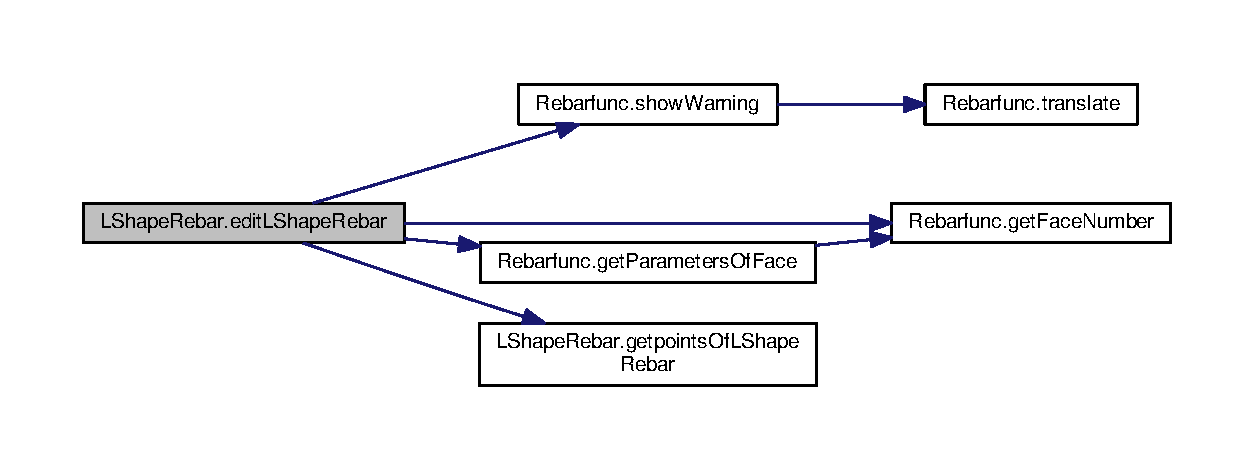
\includegraphics[width=350pt]{namespaceLShapeRebar_a9915291e3457e1c27f556d7903e02486_cgraph}
\end{center}
\end{figure}




Here is the caller graph for this function\+:\nopagebreak
\begin{figure}[H]
\begin{center}
\leavevmode
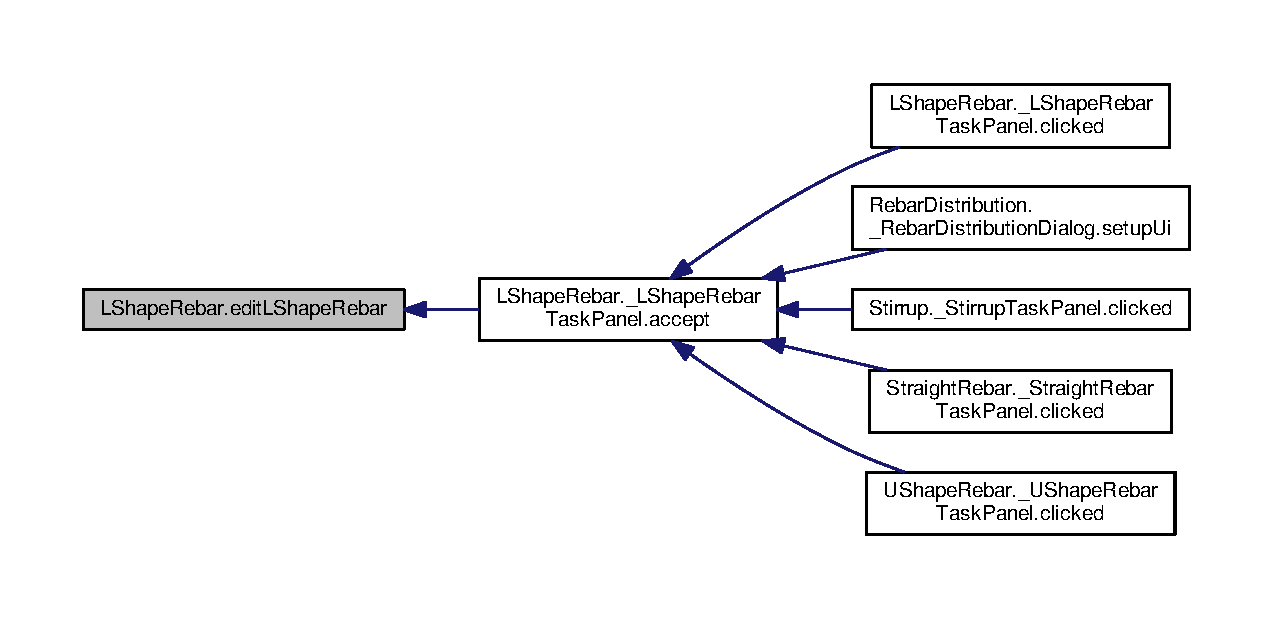
\includegraphics[width=350pt]{namespaceLShapeRebar_a9915291e3457e1c27f556d7903e02486_icgraph}
\end{center}
\end{figure}


\index{L\+Shape\+Rebar@{L\+Shape\+Rebar}!getpoints\+Of\+L\+Shape\+Rebar@{getpoints\+Of\+L\+Shape\+Rebar}}
\index{getpoints\+Of\+L\+Shape\+Rebar@{getpoints\+Of\+L\+Shape\+Rebar}!L\+Shape\+Rebar@{L\+Shape\+Rebar}}
\subsubsection[{\texorpdfstring{getpoints\+Of\+L\+Shape\+Rebar(\+Face\+P\+R\+M, l\+\_\+cover, r\+\_\+cover, b\+\_\+cover, t\+\_\+cover, orientation)}{getpointsOfLShapeRebar(FacePRM, l_cover, r_cover, b_cover, t_cover, orientation)}}]{\setlength{\rightskip}{0pt plus 5cm}def L\+Shape\+Rebar.\+getpoints\+Of\+L\+Shape\+Rebar (
\begin{DoxyParamCaption}
\item[{}]{Face\+P\+RM, }
\item[{}]{l\+\_\+cover, }
\item[{}]{r\+\_\+cover, }
\item[{}]{b\+\_\+cover, }
\item[{}]{t\+\_\+cover, }
\item[{}]{orientation}
\end{DoxyParamCaption}
)}\hypertarget{namespaceLShapeRebar_a3019960c6f6476cb70df9ee06f330dfb}{}\label{namespaceLShapeRebar_a3019960c6f6476cb70df9ee06f330dfb}
\begin{DoxyVerb}getpointsOfLShapeRebar(FacePRM, LeftCover, RightCover, BottomCover, TopCover, Orientation):
Return points of the LShape rebar in the form of array for sketch.
It takes four different orientations input i.e. 'Bottom Left', 'Bottom Right ', 'Top Left', 'Top Right'.
\end{DoxyVerb}
 

Definition at line \hyperlink{LShapeRebar_8py_source_l00040}{40} of file \hyperlink{LShapeRebar_8py_source}{L\+Shape\+Rebar.\+py}.


\begin{DoxyCode}
\hypertarget{namespaceLShapeRebar.tex_l00040}{}\hyperlink{namespaceLShapeRebar_a3019960c6f6476cb70df9ee06f330dfb}{00040} \textcolor{keyword}{def }\hyperlink{namespaceLShapeRebar_a3019960c6f6476cb70df9ee06f330dfb}{getpointsOfLShapeRebar}(FacePRM, l\_cover, r\_cover, b\_cover, t\_cover, orientation):
00041     \textcolor{stringliteral}{""" getpointsOfLShapeRebar(FacePRM, LeftCover, RightCover, BottomCover, TopCover, Orientation):}
00042 \textcolor{stringliteral}{    Return points of the LShape rebar in the form of array for sketch.}
00043 \textcolor{stringliteral}{    It takes four different orientations input i.e. 'Bottom Left', 'Bottom Right ', 'Top Left', 'Top Right'
      .}
00044 \textcolor{stringliteral}{    """}
00045     \textcolor{keywordflow}{if} orientation == \textcolor{stringliteral}{"Bottom Left"}:
00046         x1 = FacePRM[1][0] - FacePRM[0][0] / 2 + l\_cover
00047         y1 = FacePRM[1][1] + FacePRM[0][1] / 2 - t\_cover
00048         x2 = FacePRM[1][0] - FacePRM[0][0] / 2 + l\_cover
00049         y2 = FacePRM[1][1] - FacePRM[0][1] / 2 + b\_cover
00050         x3 = FacePRM[1][0] - FacePRM[0][0] / 2 + FacePRM[0][0] - r\_cover
00051         y3 = FacePRM[1][1] - FacePRM[0][1] / 2 + b\_cover
00052     \textcolor{keywordflow}{elif} orientation == \textcolor{stringliteral}{"Bottom Right"}:
00053         x1 = FacePRM[1][0] - FacePRM[0][0] / 2 + FacePRM[0][0] - r\_cover
00054         y1 = FacePRM[1][1] + FacePRM[0][1] / 2 - t\_cover
00055         x2 = FacePRM[1][0] - FacePRM[0][0] / 2 + FacePRM[0][0] - r\_cover
00056         y2 = FacePRM[1][1] - FacePRM[0][1] / 2 + b\_cover
00057         x3 = FacePRM[1][0] - FacePRM[0][0] / 2 + l\_cover
00058         y3 = FacePRM[1][1] - FacePRM[0][1] / 2 + b\_cover
00059     \textcolor{keywordflow}{elif} orientation == \textcolor{stringliteral}{"Top Left"}:
00060         x1 = FacePRM[1][0] - FacePRM[0][0] / 2 + l\_cover
00061         y1 = FacePRM[1][1] - FacePRM[0][1] / 2 + b\_cover
00062         x2 = FacePRM[1][0] - FacePRM[0][0] / 2 + l\_cover
00063         y2 = FacePRM[1][1] + FacePRM[0][1] / 2 - t\_cover
00064         x3 = FacePRM[1][0] - FacePRM[0][0] / 2 + FacePRM[0][0] - r\_cover
00065         y3 = FacePRM[1][1] + FacePRM[0][1] / 2 - t\_cover
00066     \textcolor{keywordflow}{elif} orientation == \textcolor{stringliteral}{"Top Right"}:
00067         x1 = FacePRM[1][0] - FacePRM[0][0] / 2 + FacePRM[0][0] - r\_cover
00068         y1 = FacePRM[1][1] - FacePRM[0][1] / 2 + b\_cover
00069         x2 = FacePRM[1][0] - FacePRM[0][0] / 2 + FacePRM[0][0] - r\_cover
00070         y2 = FacePRM[1][1] + FacePRM[0][1] / 2 - t\_cover
00071         x3 = FacePRM[1][0] - FacePRM[0][0] / 2 + l\_cover
00072         y3 = FacePRM[1][1] + FacePRM[0][1] / 2 - t\_cover
00073     \textcolor{keywordflow}{return} [FreeCAD.Vector(x1, y1, 0), FreeCAD.Vector(x2, y2, 0),\(\backslash\)
00074            FreeCAD.Vector(x3, y3, 0)]
00075 
\end{DoxyCode}


Here is the caller graph for this function\+:\nopagebreak
\begin{figure}[H]
\begin{center}
\leavevmode
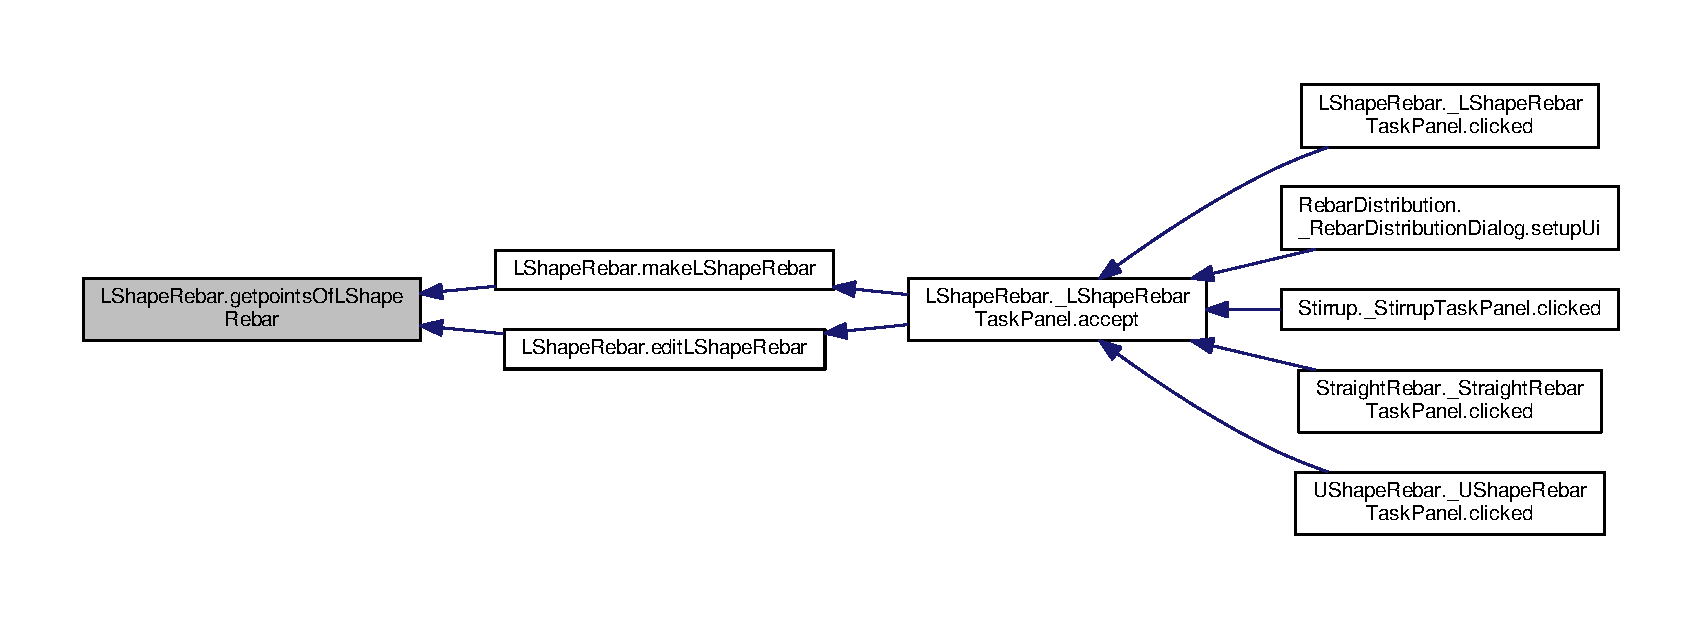
\includegraphics[width=350pt]{namespaceLShapeRebar_a3019960c6f6476cb70df9ee06f330dfb_icgraph}
\end{center}
\end{figure}


\index{L\+Shape\+Rebar@{L\+Shape\+Rebar}!make\+L\+Shape\+Rebar@{make\+L\+Shape\+Rebar}}
\index{make\+L\+Shape\+Rebar@{make\+L\+Shape\+Rebar}!L\+Shape\+Rebar@{L\+Shape\+Rebar}}
\subsubsection[{\texorpdfstring{make\+L\+Shape\+Rebar(f\+\_\+cover, b\+\_\+cover, l\+\_\+cover, r\+\_\+cover, diameter, t\+\_\+cover, rounding, amount\+\_\+spacing\+\_\+check, amount\+\_\+spacing\+\_\+value, orientation=""Bottom Left"", structure=\+None, facename=\+None)}{makeLShapeRebar(f_cover, b_cover, l_cover, r_cover, diameter, t_cover, rounding, amount_spacing_check, amount_spacing_value, orientation="Bottom Left", structure=None, facename=None)}}]{\setlength{\rightskip}{0pt plus 5cm}def L\+Shape\+Rebar.\+make\+L\+Shape\+Rebar (
\begin{DoxyParamCaption}
\item[{}]{f\+\_\+cover, }
\item[{}]{b\+\_\+cover, }
\item[{}]{l\+\_\+cover, }
\item[{}]{r\+\_\+cover, }
\item[{}]{diameter, }
\item[{}]{t\+\_\+cover, }
\item[{}]{rounding, }
\item[{}]{amount\+\_\+spacing\+\_\+check, }
\item[{}]{amount\+\_\+spacing\+\_\+value, }
\item[{}]{orientation = {\ttfamily \char`\"{}Bottom~Left\char`\"{}}, }
\item[{}]{structure = {\ttfamily None}, }
\item[{}]{facename = {\ttfamily None}}
\end{DoxyParamCaption}
)}\hypertarget{namespaceLShapeRebar_a647a28e94933108c6617da8532d76998}{}\label{namespaceLShapeRebar_a647a28e94933108c6617da8532d76998}
\begin{DoxyVerb}makeLShapeRebar(FrontCover, BottomCover, LeftCover, RightCover, Diameter, TopCover, Rounding, AmountSpacingCheck, AmountSpacingValue,
Orientation, Structure, Facename): Adds the L-Shape reinforcement bar to the selected structural object.
It takes four different orientations input i.e. 'Bottom Left', 'Bottom Right ', 'Top Left', 'Top Right'.
\end{DoxyVerb}
 

Definition at line \hyperlink{LShapeRebar_8py_source_l00169}{169} of file \hyperlink{LShapeRebar_8py_source}{L\+Shape\+Rebar.\+py}.


\begin{DoxyCode}
\hypertarget{namespaceLShapeRebar.tex_l00169}{}\hyperlink{namespaceLShapeRebar_a647a28e94933108c6617da8532d76998}{00169} \textcolor{keyword}{def }\hyperlink{namespaceLShapeRebar_a647a28e94933108c6617da8532d76998}{makeLShapeRebar}(f\_cover, b\_cover, l\_cover, r\_cover, diameter, t\_cover, rounding, 
      amount\_spacing\_check, amount\_spacing\_value, orientation = "Bottom Left", structure = None, facename = None):
00170     \textcolor{stringliteral}{""" makeLShapeRebar(FrontCover, BottomCover, LeftCover, RightCover, Diameter, TopCover, Rounding,
       AmountSpacingCheck, AmountSpacingValue,}
00171 \textcolor{stringliteral}{    Orientation, Structure, Facename): Adds the L-Shape reinforcement bar to the selected structural
       object.}
00172 \textcolor{stringliteral}{    It takes four different orientations input i.e. 'Bottom Left', 'Bottom Right ', 'Top Left', 'Top Right'
      .}
00173 \textcolor{stringliteral}{    """}
00174     \textcolor{keywordflow}{if} \textcolor{keywordflow}{not} structure \textcolor{keywordflow}{and} \textcolor{keywordflow}{not} facename:
00175         selected\_obj = FreeCADGui.Selection.getSelectionEx()[0]
00176         structure = selected\_obj.Object
00177         facename = selected\_obj.SubElementNames[0]
00178     face = structure.Shape.Faces[\hyperlink{namespaceRebarfunc_a3885b3b63e3a41508ac79bc7550cf301}{getFaceNumber}(facename) - 1]
00179     \textcolor{comment}{#StructurePRM = getTrueParametersOfStructure(structure)}
00180     FacePRM = \hyperlink{namespaceRebarfunc_a92122b3d7cedd3d47bb63380a5ac4d08}{getParametersOfFace}(structure, facename)
00181     \textcolor{keywordflow}{if} \textcolor{keywordflow}{not} FacePRM:
00182         FreeCAD.Console.PrintError(\textcolor{stringliteral}{"Cannot identified shape or from which base object sturctural element is
       derived\(\backslash\)n"})
00183         \textcolor{keywordflow}{return}
00184     \textcolor{comment}{# Get points of L-Shape rebar}
00185     points = \hyperlink{namespaceLShapeRebar_a3019960c6f6476cb70df9ee06f330dfb}{getpointsOfLShapeRebar}(FacePRM, l\_cover, r\_cover, b\_cover, t\_cover, 
      orientation)
00186     \textcolor{keyword}{import} Part
00187     \textcolor{keyword}{import} Arch
00188     sketch = FreeCAD.activeDocument().addObject(\textcolor{stringliteral}{'Sketcher::SketchObject'}, \textcolor{stringliteral}{'Sketch'})
00189     sketch.MapMode = \textcolor{stringliteral}{"FlatFace"}
00190     sketch.Support = [(structure, facename)]
00191     FreeCAD.ActiveDocument.recompute()
00192     sketch.addGeometry(Part.LineSegment(points[0], points[1]), \textcolor{keyword}{False})
00193     sketch.addGeometry(Part.LineSegment(points[1], points[2]), \textcolor{keyword}{False})
00194     \textcolor{keyword}{import} Sketcher
00195     \textcolor{keywordflow}{if} amount\_spacing\_check:
00196         rebar = Arch.makeRebar(structure, sketch, diameter, amount\_spacing\_value, f\_cover)
00197         FreeCAD.ActiveDocument.recompute()
00198     \textcolor{keywordflow}{else}:
00199         size = (ArchCommands.projectToVector(structure.Shape.copy(), face.normalAt(0, 0))).Length
00200         rebar = Arch.makeRebar(structure, sketch, diameter, int((size - diameter) / amount\_spacing\_value), 
      f\_cover)
00201     rebar.Rounding = rounding
00202     \textcolor{comment}{# Adds properties to the rebar object}
00203     rebar.ViewObject.addProperty(\textcolor{stringliteral}{"App::PropertyString"}, \textcolor{stringliteral}{"RebarShape"}, \textcolor{stringliteral}{"RebarDialog"}, QT\_TRANSLATE\_NOOP(\textcolor{stringliteral}{"
      App::Property"}, \textcolor{stringliteral}{"Shape of rebar"})).RebarShape = \textcolor{stringliteral}{"LShapeRebar"}
00204     rebar.ViewObject.setEditorMode(\textcolor{stringliteral}{"RebarShape"}, 2)
00205     rebar.addProperty(\textcolor{stringliteral}{"App::PropertyDistance"}, \textcolor{stringliteral}{"FrontCover"}, \textcolor{stringliteral}{"RebarDialog"}, QT\_TRANSLATE\_NOOP(\textcolor{stringliteral}{"
      App::Property"}, \textcolor{stringliteral}{"Front cover of rebar"})).FrontCover = f\_cover
00206     rebar.setEditorMode(\textcolor{stringliteral}{"FrontCover"}, 2)
00207     rebar.addProperty(\textcolor{stringliteral}{"App::PropertyDistance"}, \textcolor{stringliteral}{"LeftCover"}, \textcolor{stringliteral}{"RebarDialog"}, QT\_TRANSLATE\_NOOP(\textcolor{stringliteral}{"App::Property
      "}, \textcolor{stringliteral}{"Left Side cover of rebar"})).LeftCover = l\_cover
00208     rebar.setEditorMode(\textcolor{stringliteral}{"LeftCover"}, 2)
00209     rebar.addProperty(\textcolor{stringliteral}{"App::PropertyDistance"}, \textcolor{stringliteral}{"RightCover"}, \textcolor{stringliteral}{"RebarDialog"}, QT\_TRANSLATE\_NOOP(\textcolor{stringliteral}{"
      App::Property"}, \textcolor{stringliteral}{"Right Side cover of rebar"})).RightCover = r\_cover
00210     rebar.setEditorMode(\textcolor{stringliteral}{"RightCover"}, 2)
00211     rebar.addProperty(\textcolor{stringliteral}{"App::PropertyDistance"}, \textcolor{stringliteral}{"BottomCover"}, \textcolor{stringliteral}{"RebarDialog"}, QT\_TRANSLATE\_NOOP(\textcolor{stringliteral}{"
      App::Property"}, \textcolor{stringliteral}{"Bottom cover of rebar"})).BottomCover = b\_cover
00212     rebar.setEditorMode(\textcolor{stringliteral}{"BottomCover"}, 2)
00213     rebar.addProperty(\textcolor{stringliteral}{"App::PropertyBool"}, \textcolor{stringliteral}{"AmountCheck"}, \textcolor{stringliteral}{"RebarDialog"}, QT\_TRANSLATE\_NOOP(\textcolor{stringliteral}{"App::Property"},
       \textcolor{stringliteral}{"Amount radio button is checked"})).AmountCheck
00214     rebar.setEditorMode(\textcolor{stringliteral}{"AmountCheck"}, 2)
00215     rebar.addProperty(\textcolor{stringliteral}{"App::PropertyDistance"}, \textcolor{stringliteral}{"TopCover"}, \textcolor{stringliteral}{"RebarDialog"}, QT\_TRANSLATE\_NOOP(\textcolor{stringliteral}{"App::Property"}
      , \textcolor{stringliteral}{"Top cover of rebar"})).TopCover = t\_cover
00216     rebar.setEditorMode(\textcolor{stringliteral}{"TopCover"}, 2)
00217     rebar.addProperty(\textcolor{stringliteral}{"App::PropertyDistance"}, \textcolor{stringliteral}{"TrueSpacing"}, \textcolor{stringliteral}{"RebarDialog"}, QT\_TRANSLATE\_NOOP(\textcolor{stringliteral}{"
      App::Property"}, \textcolor{stringliteral}{"Spacing between of rebars"})).TrueSpacing = amount\_spacing\_value
00218     rebar.addProperty(\textcolor{stringliteral}{"App::PropertyString"}, \textcolor{stringliteral}{"Orientation"}, \textcolor{stringliteral}{"RebarDialog"}, QT\_TRANSLATE\_NOOP(\textcolor{stringliteral}{"App::Property
      "}, \textcolor{stringliteral}{"Shape of rebar"})).Orientation = orientation
00219     rebar.setEditorMode(\textcolor{stringliteral}{"Orientation"}, 2)
00220     rebar.setEditorMode(\textcolor{stringliteral}{"TrueSpacing"}, 2)
00221     \textcolor{keywordflow}{if} amount\_spacing\_check:
00222         rebar.AmountCheck = \textcolor{keyword}{True}
00223     \textcolor{keywordflow}{else}:
00224         rebar.AmountCheck = \textcolor{keyword}{False}
00225         rebar.TrueSpacing = amount\_spacing\_value
00226     rebar.Label = \textcolor{stringliteral}{"LShapeRebar"}
00227     FreeCAD.ActiveDocument.recompute()
00228     \textcolor{keywordflow}{return} rebar
00229 
\end{DoxyCode}


Here is the call graph for this function\+:\nopagebreak
\begin{figure}[H]
\begin{center}
\leavevmode
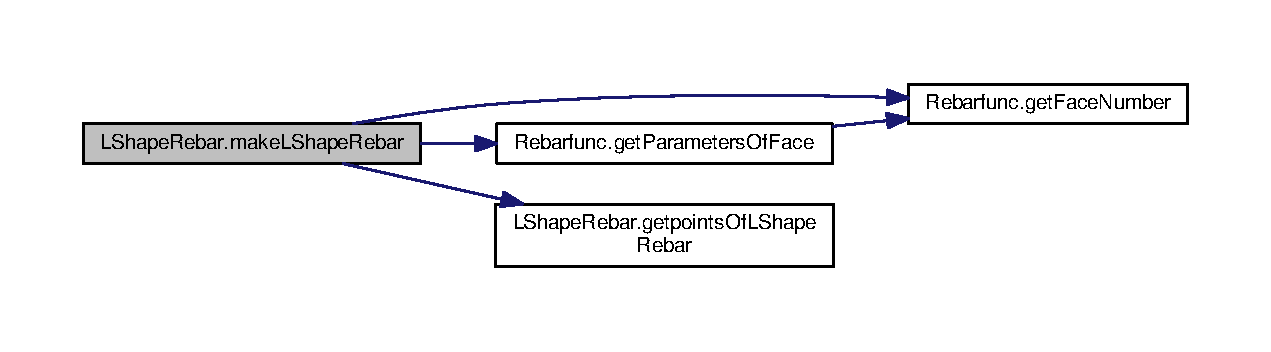
\includegraphics[width=350pt]{namespaceLShapeRebar_a647a28e94933108c6617da8532d76998_cgraph}
\end{center}
\end{figure}




Here is the caller graph for this function\+:\nopagebreak
\begin{figure}[H]
\begin{center}
\leavevmode
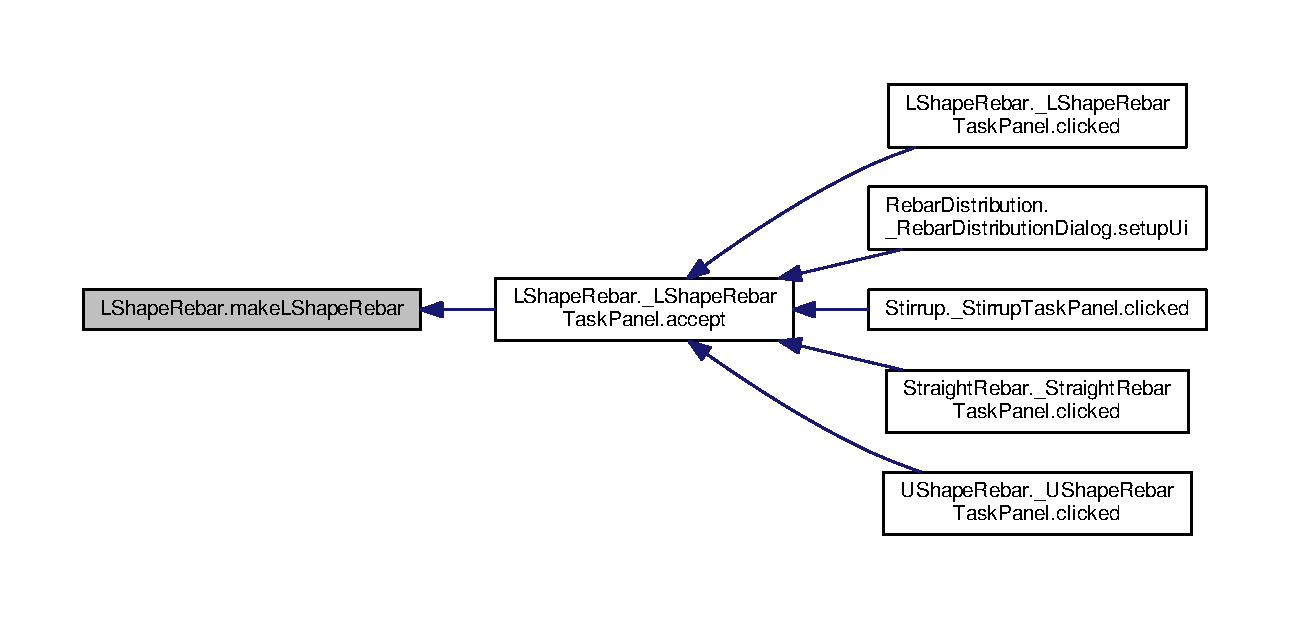
\includegraphics[width=350pt]{namespaceLShapeRebar_a647a28e94933108c6617da8532d76998_icgraph}
\end{center}
\end{figure}




\subsection{Variable Documentation}
\index{L\+Shape\+Rebar@{L\+Shape\+Rebar}!\+\_\+\+\_\+author\+\_\+\+\_\+@{\+\_\+\+\_\+author\+\_\+\+\_\+}}
\index{\+\_\+\+\_\+author\+\_\+\+\_\+@{\+\_\+\+\_\+author\+\_\+\+\_\+}!L\+Shape\+Rebar@{L\+Shape\+Rebar}}
\subsubsection[{\texorpdfstring{\+\_\+\+\_\+author\+\_\+\+\_\+}{__author__}}]{\setlength{\rightskip}{0pt plus 5cm}string L\+Shape\+Rebar.\+\_\+\+\_\+author\+\_\+\+\_\+ = \char`\"{}Amritpal Singh\char`\"{}\hspace{0.3cm}{\ttfamily [private]}}\hypertarget{namespaceLShapeRebar_ad398517c2df8a455dfd0b670e54285ea}{}\label{namespaceLShapeRebar_ad398517c2df8a455dfd0b670e54285ea}


Definition at line \hyperlink{LShapeRebar_8py_source_l00025}{25} of file \hyperlink{LShapeRebar_8py_source}{L\+Shape\+Rebar.\+py}.

\index{L\+Shape\+Rebar@{L\+Shape\+Rebar}!\+\_\+\+\_\+title\+\_\+\+\_\+@{\+\_\+\+\_\+title\+\_\+\+\_\+}}
\index{\+\_\+\+\_\+title\+\_\+\+\_\+@{\+\_\+\+\_\+title\+\_\+\+\_\+}!L\+Shape\+Rebar@{L\+Shape\+Rebar}}
\subsubsection[{\texorpdfstring{\+\_\+\+\_\+title\+\_\+\+\_\+}{__title__}}]{\setlength{\rightskip}{0pt plus 5cm}string L\+Shape\+Rebar.\+\_\+\+\_\+title\+\_\+\+\_\+ = \char`\"{}L\+Shape\+Rebar\char`\"{}\hspace{0.3cm}{\ttfamily [private]}}\hypertarget{namespaceLShapeRebar_a0ac8e9cb97e560c6ce362c1ac5144c31}{}\label{namespaceLShapeRebar_a0ac8e9cb97e560c6ce362c1ac5144c31}


Definition at line \hyperlink{LShapeRebar_8py_source_l00024}{24} of file \hyperlink{LShapeRebar_8py_source}{L\+Shape\+Rebar.\+py}.

\index{L\+Shape\+Rebar@{L\+Shape\+Rebar}!\+\_\+\+\_\+url\+\_\+\+\_\+@{\+\_\+\+\_\+url\+\_\+\+\_\+}}
\index{\+\_\+\+\_\+url\+\_\+\+\_\+@{\+\_\+\+\_\+url\+\_\+\+\_\+}!L\+Shape\+Rebar@{L\+Shape\+Rebar}}
\subsubsection[{\texorpdfstring{\+\_\+\+\_\+url\+\_\+\+\_\+}{__url__}}]{\setlength{\rightskip}{0pt plus 5cm}string L\+Shape\+Rebar.\+\_\+\+\_\+url\+\_\+\+\_\+ = \char`\"{}https\+://www.\+freecadweb.\+org\char`\"{}\hspace{0.3cm}{\ttfamily [private]}}\hypertarget{namespaceLShapeRebar_a7bca929f0dda68928d1f3978b4e877f8}{}\label{namespaceLShapeRebar_a7bca929f0dda68928d1f3978b4e877f8}


Definition at line \hyperlink{LShapeRebar_8py_source_l00026}{26} of file \hyperlink{LShapeRebar_8py_source}{L\+Shape\+Rebar.\+py}.


\hypertarget{namespacePopUpImage}{}\section{Pop\+Up\+Image Namespace Reference}
\label{namespacePopUpImage}\index{Pop\+Up\+Image@{Pop\+Up\+Image}}
\subsection*{Classes}
\begin{DoxyCompactItemize}
\item 
class \hyperlink{classPopUpImage_1_1PopUpImage}{Pop\+Up\+Image}
\end{DoxyCompactItemize}
\subsection*{Functions}
\begin{DoxyCompactItemize}
\item 
def \hyperlink{namespacePopUpImage_a8c565620d7de9b4882a44eacb870ad05}{show\+Pop\+Up\+Image\+Dialog} (img)
\end{DoxyCompactItemize}
\subsection*{Variables}
\begin{DoxyCompactItemize}
\item 
string \hyperlink{namespacePopUpImage_a4141c27e055e2d28a4b83ce4a05c56f1}{\+\_\+\+\_\+title\+\_\+\+\_\+} = \char`\"{}Pop\+Up\+Image\char`\"{}
\item 
string \hyperlink{namespacePopUpImage_ad3422bf98333fc29e0ca232e088d99c3}{\+\_\+\+\_\+author\+\_\+\+\_\+} = \char`\"{}Amritpal Singh\char`\"{}
\item 
string \hyperlink{namespacePopUpImage_a5c155cc535acd99cd7c1179185e9c857}{\+\_\+\+\_\+url\+\_\+\+\_\+} = \char`\"{}https\+://www.\+freecadweb.\+org\char`\"{}
\end{DoxyCompactItemize}


\subsection{Function Documentation}
\index{Pop\+Up\+Image@{Pop\+Up\+Image}!show\+Pop\+Up\+Image\+Dialog@{show\+Pop\+Up\+Image\+Dialog}}
\index{show\+Pop\+Up\+Image\+Dialog@{show\+Pop\+Up\+Image\+Dialog}!Pop\+Up\+Image@{Pop\+Up\+Image}}
\subsubsection[{\texorpdfstring{show\+Pop\+Up\+Image\+Dialog(img)}{showPopUpImageDialog(img)}}]{\setlength{\rightskip}{0pt plus 5cm}def Pop\+Up\+Image.\+show\+Pop\+Up\+Image\+Dialog (
\begin{DoxyParamCaption}
\item[{}]{img}
\end{DoxyParamCaption}
)}\hypertarget{namespacePopUpImage_a8c565620d7de9b4882a44eacb870ad05}{}\label{namespacePopUpImage_a8c565620d7de9b4882a44eacb870ad05}
\begin{DoxyVerb}showPopUpImageDialog(image): This function will show a given image in a pop-up
dialog box.\end{DoxyVerb}
 

Definition at line \hyperlink{PopUpImage_8py_source_l00043}{43} of file \hyperlink{PopUpImage_8py_source}{Pop\+Up\+Image.\+py}.


\begin{DoxyCode}
\hypertarget{namespacePopUpImage.tex_l00043}{}\hyperlink{namespacePopUpImage_a8c565620d7de9b4882a44eacb870ad05}{00043} \textcolor{keyword}{def }\hyperlink{namespacePopUpImage_a8c565620d7de9b4882a44eacb870ad05}{showPopUpImageDialog}(img):
00044     \textcolor{stringliteral}{""" showPopUpImageDialog(image): This function will show a given image in a pop-up}
00045 \textcolor{stringliteral}{    dialog box."""}
00046     dialog = \hyperlink{classPopUpImage_1_1PopUpImage}{PopUpImage}(img)
00047     dialog.exec\_()
00048 \end{DoxyCode}


\subsection{Variable Documentation}
\index{Pop\+Up\+Image@{Pop\+Up\+Image}!\+\_\+\+\_\+author\+\_\+\+\_\+@{\+\_\+\+\_\+author\+\_\+\+\_\+}}
\index{\+\_\+\+\_\+author\+\_\+\+\_\+@{\+\_\+\+\_\+author\+\_\+\+\_\+}!Pop\+Up\+Image@{Pop\+Up\+Image}}
\subsubsection[{\texorpdfstring{\+\_\+\+\_\+author\+\_\+\+\_\+}{__author__}}]{\setlength{\rightskip}{0pt plus 5cm}string Pop\+Up\+Image.\+\_\+\+\_\+author\+\_\+\+\_\+ = \char`\"{}Amritpal Singh\char`\"{}\hspace{0.3cm}{\ttfamily [private]}}\hypertarget{namespacePopUpImage_ad3422bf98333fc29e0ca232e088d99c3}{}\label{namespacePopUpImage_ad3422bf98333fc29e0ca232e088d99c3}


Definition at line \hyperlink{PopUpImage_8py_source_l00025}{25} of file \hyperlink{PopUpImage_8py_source}{Pop\+Up\+Image.\+py}.

\index{Pop\+Up\+Image@{Pop\+Up\+Image}!\+\_\+\+\_\+title\+\_\+\+\_\+@{\+\_\+\+\_\+title\+\_\+\+\_\+}}
\index{\+\_\+\+\_\+title\+\_\+\+\_\+@{\+\_\+\+\_\+title\+\_\+\+\_\+}!Pop\+Up\+Image@{Pop\+Up\+Image}}
\subsubsection[{\texorpdfstring{\+\_\+\+\_\+title\+\_\+\+\_\+}{__title__}}]{\setlength{\rightskip}{0pt plus 5cm}string Pop\+Up\+Image.\+\_\+\+\_\+title\+\_\+\+\_\+ = \char`\"{}Pop\+Up\+Image\char`\"{}\hspace{0.3cm}{\ttfamily [private]}}\hypertarget{namespacePopUpImage_a4141c27e055e2d28a4b83ce4a05c56f1}{}\label{namespacePopUpImage_a4141c27e055e2d28a4b83ce4a05c56f1}


Definition at line \hyperlink{PopUpImage_8py_source_l00024}{24} of file \hyperlink{PopUpImage_8py_source}{Pop\+Up\+Image.\+py}.

\index{Pop\+Up\+Image@{Pop\+Up\+Image}!\+\_\+\+\_\+url\+\_\+\+\_\+@{\+\_\+\+\_\+url\+\_\+\+\_\+}}
\index{\+\_\+\+\_\+url\+\_\+\+\_\+@{\+\_\+\+\_\+url\+\_\+\+\_\+}!Pop\+Up\+Image@{Pop\+Up\+Image}}
\subsubsection[{\texorpdfstring{\+\_\+\+\_\+url\+\_\+\+\_\+}{__url__}}]{\setlength{\rightskip}{0pt plus 5cm}string Pop\+Up\+Image.\+\_\+\+\_\+url\+\_\+\+\_\+ = \char`\"{}https\+://www.\+freecadweb.\+org\char`\"{}\hspace{0.3cm}{\ttfamily [private]}}\hypertarget{namespacePopUpImage_a5c155cc535acd99cd7c1179185e9c857}{}\label{namespacePopUpImage_a5c155cc535acd99cd7c1179185e9c857}


Definition at line \hyperlink{PopUpImage_8py_source_l00026}{26} of file \hyperlink{PopUpImage_8py_source}{Pop\+Up\+Image.\+py}.


\hypertarget{namespaceRebarDistribution}{}\section{Rebar\+Distribution Namespace Reference}
\label{namespaceRebarDistribution}\index{Rebar\+Distribution@{Rebar\+Distribution}}
\subsection*{Classes}
\begin{DoxyCompactItemize}
\item 
class \hyperlink{classRebarDistribution_1_1__RebarDistributionDialog}{\+\_\+\+Rebar\+Distribution\+Dialog}
\end{DoxyCompactItemize}
\subsection*{Functions}
\begin{DoxyCompactItemize}
\item 
def \hyperlink{namespaceRebarDistribution_a22a12f260218752c4099cf68e4e3da5c}{get\+Custom\+Spacing\+String} (amount1, spacing1, amount2, spacing2, amount3, spacing3, front\+Cover, size)
\item 
def \hyperlink{namespaceRebarDistribution_a59ac567a8536ea3b5e7a9900a898e0c0}{getuple\+Of\+Custom\+Spacing} (span\+\_\+string)
\item 
def \hyperlink{namespaceRebarDistribution_aa547df5cb10d2e64eaa0b51c445fa30b}{run\+Rebar\+Distribution} (self)
\item 
def \hyperlink{namespaceRebarDistribution_a85270a1b6e8c782a9e0ba54add518f2a}{remove\+Rebar\+Distribution} (self)
\end{DoxyCompactItemize}
\subsection*{Variables}
\begin{DoxyCompactItemize}
\item 
string \hyperlink{namespaceRebarDistribution_a38609d6513215400fb6b4c0d1b7f2040}{\+\_\+\+\_\+title\+\_\+\+\_\+} = \char`\"{}Dialog\+Distribution\char`\"{}
\item 
string \hyperlink{namespaceRebarDistribution_a7bd0602448fa39ff800847e313ca8b25}{\+\_\+\+\_\+author\+\_\+\+\_\+} = \char`\"{}Amritpal Singh\char`\"{}
\item 
string \hyperlink{namespaceRebarDistribution_a61d261a603c7a127f83af9b7516547c5}{\+\_\+\+\_\+url\+\_\+\+\_\+} = \char`\"{}https\+://www.\+freecadweb.\+org\char`\"{}
\item 
\hyperlink{namespaceRebarDistribution_a6572ac63b9c553f99eeb53e19f7b4e7c}{Custom\+Spacing}
\end{DoxyCompactItemize}


\subsection{Function Documentation}
\index{Rebar\+Distribution@{Rebar\+Distribution}!get\+Custom\+Spacing\+String@{get\+Custom\+Spacing\+String}}
\index{get\+Custom\+Spacing\+String@{get\+Custom\+Spacing\+String}!Rebar\+Distribution@{Rebar\+Distribution}}
\subsubsection[{\texorpdfstring{get\+Custom\+Spacing\+String(amount1, spacing1, amount2, spacing2, amount3, spacing3, front\+Cover, size)}{getCustomSpacingString(amount1, spacing1, amount2, spacing2, amount3, spacing3, frontCover, size)}}]{\setlength{\rightskip}{0pt plus 5cm}def Rebar\+Distribution.\+get\+Custom\+Spacing\+String (
\begin{DoxyParamCaption}
\item[{}]{amount1, }
\item[{}]{spacing1, }
\item[{}]{amount2, }
\item[{}]{spacing2, }
\item[{}]{amount3, }
\item[{}]{spacing3, }
\item[{}]{front\+Cover, }
\item[{}]{size}
\end{DoxyParamCaption}
)}\hypertarget{namespaceRebarDistribution_a22a12f260218752c4099cf68e4e3da5c}{}\label{namespaceRebarDistribution_a22a12f260218752c4099cf68e4e3da5c}


Definition at line \hyperlink{RebarDistribution_8py_source_l00063}{63} of file \hyperlink{RebarDistribution_8py_source}{Rebar\+Distribution.\+py}.


\begin{DoxyCode}
\hypertarget{namespaceRebarDistribution.tex_l00063}{}\hyperlink{namespaceRebarDistribution_a22a12f260218752c4099cf68e4e3da5c}{00063} \textcolor{keyword}{def }\hyperlink{namespaceRebarDistribution_a22a12f260218752c4099cf68e4e3da5c}{getCustomSpacingString}(amount1, spacing1, amount2, spacing2, amount3, spacing3, 
      frontCover, size):
00064     seg1\_area = amount1 * spacing1 - spacing1 / 2
00065     seg3\_area = amount3 * spacing3 - spacing3 / 2
00066     seg2\_area = size - seg1\_area - seg3\_area - 2 * frontCover
00067     \textcolor{keywordflow}{if} seg2\_area < 0:
00068         FreeCAD.Console.PrintError(\textcolor{stringliteral}{"Sum of length of segment 1 and segment 2 is greater than length of
       rebar expands.\(\backslash\)n"})
00069         \textcolor{keywordflow}{return}
00070     \textcolor{keywordflow}{if} spacing1 \textcolor{keywordflow}{and} spacing2 \textcolor{keywordflow}{and} spacing3 \textcolor{keywordflow}{and} amount1 \textcolor{keywordflow}{and} amount2 \textcolor{keywordflow}{and} amount3:
00071         \textcolor{keywordflow}{pass}
00072     \textcolor{keywordflow}{else}:
00073         \textcolor{keywordflow}{if} spacing1 \textcolor{keywordflow}{and} spacing2 \textcolor{keywordflow}{and} spacing3:
00074             amount2 = math.ceil(seg2\_area / spacing2)
00075             spacing2 = seg2\_area / amount2
00076         \textcolor{keywordflow}{elif} amount1 \textcolor{keywordflow}{and} amount2 \textcolor{keywordflow}{and} amount3:
00077             spacing2 = math.floor(seg2\_area / amount2)
00078     CustomSpacing = str(amount1) + \textcolor{stringliteral}{"@"} + str(spacing1) + \textcolor{stringliteral}{"+"} + str(int(amount2)) + \textcolor{stringliteral}{"@"} + str(spacing2) + \textcolor{stringliteral}{"+
      "} + str(amount3) + \textcolor{stringliteral}{"@"} + str(spacing3)
00079     \textcolor{keywordflow}{return} CustomSpacing
00080 
\end{DoxyCode}
\index{Rebar\+Distribution@{Rebar\+Distribution}!getuple\+Of\+Custom\+Spacing@{getuple\+Of\+Custom\+Spacing}}
\index{getuple\+Of\+Custom\+Spacing@{getuple\+Of\+Custom\+Spacing}!Rebar\+Distribution@{Rebar\+Distribution}}
\subsubsection[{\texorpdfstring{getuple\+Of\+Custom\+Spacing(span\+\_\+string)}{getupleOfCustomSpacing(span_string)}}]{\setlength{\rightskip}{0pt plus 5cm}def Rebar\+Distribution.\+getuple\+Of\+Custom\+Spacing (
\begin{DoxyParamCaption}
\item[{}]{span\+\_\+string}
\end{DoxyParamCaption}
)}\hypertarget{namespaceRebarDistribution_a59ac567a8536ea3b5e7a9900a898e0c0}{}\label{namespaceRebarDistribution_a59ac567a8536ea3b5e7a9900a898e0c0}
\begin{DoxyVerb}gettupleOfCustomSpacing(span_string): This function take input
in specific syntax and return output in the form of list. For eg.
Input: "3@100+2@200+3@100"
Output: [(3, 100), (2, 200), (3, 100)]\end{DoxyVerb}
 

Definition at line \hyperlink{RebarDistribution_8py_source_l00081}{81} of file \hyperlink{RebarDistribution_8py_source}{Rebar\+Distribution.\+py}.


\begin{DoxyCode}
\hypertarget{namespaceRebarDistribution.tex_l00081}{}\hyperlink{namespaceRebarDistribution_a59ac567a8536ea3b5e7a9900a898e0c0}{00081} \textcolor{keyword}{def }\hyperlink{namespaceRebarDistribution_a59ac567a8536ea3b5e7a9900a898e0c0}{getupleOfCustomSpacing}(span\_string):
00082     \textcolor{stringliteral}{""" gettupleOfCustomSpacing(span\_string): This function take input}
00083 \textcolor{stringliteral}{    in specific syntax and return output in the form of list. For eg.}
00084 \textcolor{stringliteral}{    Input: "3@100+2@200+3@100"}
00085 \textcolor{stringliteral}{    Output: [(3, 100), (2, 200), (3, 100)]"""}
00086     \textcolor{keyword}{import} string
00087     span\_st = string.strip(span\_string)
00088     span\_sp = string.split(span\_st, \textcolor{stringliteral}{'+'})
00089     index = 0
00090     spacinglist = []
00091     \textcolor{keywordflow}{while} index < len(span\_sp):
00092         \textcolor{comment}{# Find "@" recursively in span\_sp array.}
00093         in\_sp = string.split(span\_sp[index], \textcolor{stringliteral}{'@'})
00094         spacinglist.append((int(in\_sp[0]),float(in\_sp[1])))
00095         index += 1
00096     \textcolor{keywordflow}{return} spacinglist
00097 
\end{DoxyCode}
\index{Rebar\+Distribution@{Rebar\+Distribution}!remove\+Rebar\+Distribution@{remove\+Rebar\+Distribution}}
\index{remove\+Rebar\+Distribution@{remove\+Rebar\+Distribution}!Rebar\+Distribution@{Rebar\+Distribution}}
\subsubsection[{\texorpdfstring{remove\+Rebar\+Distribution(self)}{removeRebarDistribution(self)}}]{\setlength{\rightskip}{0pt plus 5cm}def Rebar\+Distribution.\+remove\+Rebar\+Distribution (
\begin{DoxyParamCaption}
\item[{}]{self}
\end{DoxyParamCaption}
)}\hypertarget{namespaceRebarDistribution_a85270a1b6e8c782a9e0ba54add518f2a}{}\label{namespaceRebarDistribution_a85270a1b6e8c782a9e0ba54add518f2a}


Definition at line \hyperlink{RebarDistribution_8py_source_l00108}{108} of file \hyperlink{RebarDistribution_8py_source}{Rebar\+Distribution.\+py}.


\begin{DoxyCode}
\hypertarget{namespaceRebarDistribution.tex_l00108}{}\hyperlink{namespaceRebarDistribution_a85270a1b6e8c782a9e0ba54add518f2a}{00108} \textcolor{keyword}{def }\hyperlink{namespaceRebarDistribution_a85270a1b6e8c782a9e0ba54add518f2a}{removeRebarDistribution}(self):
00109     self.CustomSpacing = \textcolor{stringliteral}{""}
00110     self.Rebar.CustomSpacing = \textcolor{stringliteral}{""}
00111     FreeCAD.ActiveDocument.recompute()
00112 
00113 \textcolor{comment}{#runRebarDistribution(App.ActiveDocument.Rebar)}
00114 \end{DoxyCode}
\index{Rebar\+Distribution@{Rebar\+Distribution}!run\+Rebar\+Distribution@{run\+Rebar\+Distribution}}
\index{run\+Rebar\+Distribution@{run\+Rebar\+Distribution}!Rebar\+Distribution@{Rebar\+Distribution}}
\subsubsection[{\texorpdfstring{run\+Rebar\+Distribution(self)}{runRebarDistribution(self)}}]{\setlength{\rightskip}{0pt plus 5cm}def Rebar\+Distribution.\+run\+Rebar\+Distribution (
\begin{DoxyParamCaption}
\item[{}]{self}
\end{DoxyParamCaption}
)}\hypertarget{namespaceRebarDistribution_aa547df5cb10d2e64eaa0b51c445fa30b}{}\label{namespaceRebarDistribution_aa547df5cb10d2e64eaa0b51c445fa30b}


Definition at line \hyperlink{RebarDistribution_8py_source_l00098}{98} of file \hyperlink{RebarDistribution_8py_source}{Rebar\+Distribution.\+py}.


\begin{DoxyCode}
\hypertarget{namespaceRebarDistribution.tex_l00098}{}\hyperlink{namespaceRebarDistribution_aa547df5cb10d2e64eaa0b51c445fa30b}{00098} \textcolor{keyword}{def }\hyperlink{namespaceRebarDistribution_aa547df5cb10d2e64eaa0b51c445fa30b}{runRebarDistribution}(self):
00099     frontCover = self.form.frontCover.text()
00100     frontCover = FreeCAD.Units.Quantity(frontCover).Value
00101     face = self.SelectedObj.Shape.Faces[\hyperlink{namespaceRebarfunc_a3885b3b63e3a41508ac79bc7550cf301}{getFaceNumber}(self.FaceName) - 1]
00102     size = (ArchCommands.projectToVector(self.SelectedObj.Shape.copy(), face.normalAt(0, 0))).Length
00103     dialog = \hyperlink{classRebarDistribution_1_1__RebarDistributionDialog}{\_RebarDistributionDialog}(frontCover, size)
00104     dialog.setupUi()
00105     dialog.form.exec\_()
\hypertarget{namespaceRebarDistribution.tex_l00106}{}\hyperlink{namespaceRebarDistribution_a6572ac63b9c553f99eeb53e19f7b4e7c}{00106}     self.CustomSpacing = dialog.CustomSpacing
00107 
\end{DoxyCode}


Here is the call graph for this function\+:\nopagebreak
\begin{figure}[H]
\begin{center}
\leavevmode
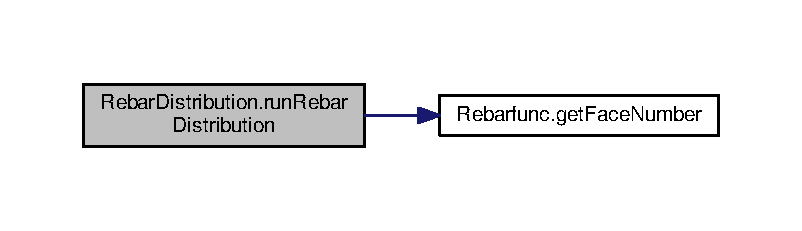
\includegraphics[width=350pt]{namespaceRebarDistribution_aa547df5cb10d2e64eaa0b51c445fa30b_cgraph}
\end{center}
\end{figure}




\subsection{Variable Documentation}
\index{Rebar\+Distribution@{Rebar\+Distribution}!\+\_\+\+\_\+author\+\_\+\+\_\+@{\+\_\+\+\_\+author\+\_\+\+\_\+}}
\index{\+\_\+\+\_\+author\+\_\+\+\_\+@{\+\_\+\+\_\+author\+\_\+\+\_\+}!Rebar\+Distribution@{Rebar\+Distribution}}
\subsubsection[{\texorpdfstring{\+\_\+\+\_\+author\+\_\+\+\_\+}{__author__}}]{\setlength{\rightskip}{0pt plus 5cm}string Rebar\+Distribution.\+\_\+\+\_\+author\+\_\+\+\_\+ = \char`\"{}Amritpal Singh\char`\"{}\hspace{0.3cm}{\ttfamily [private]}}\hypertarget{namespaceRebarDistribution_a7bd0602448fa39ff800847e313ca8b25}{}\label{namespaceRebarDistribution_a7bd0602448fa39ff800847e313ca8b25}


Definition at line \hyperlink{RebarDistribution_8py_source_l00025}{25} of file \hyperlink{RebarDistribution_8py_source}{Rebar\+Distribution.\+py}.

\index{Rebar\+Distribution@{Rebar\+Distribution}!\+\_\+\+\_\+title\+\_\+\+\_\+@{\+\_\+\+\_\+title\+\_\+\+\_\+}}
\index{\+\_\+\+\_\+title\+\_\+\+\_\+@{\+\_\+\+\_\+title\+\_\+\+\_\+}!Rebar\+Distribution@{Rebar\+Distribution}}
\subsubsection[{\texorpdfstring{\+\_\+\+\_\+title\+\_\+\+\_\+}{__title__}}]{\setlength{\rightskip}{0pt plus 5cm}string Rebar\+Distribution.\+\_\+\+\_\+title\+\_\+\+\_\+ = \char`\"{}Dialog\+Distribution\char`\"{}\hspace{0.3cm}{\ttfamily [private]}}\hypertarget{namespaceRebarDistribution_a38609d6513215400fb6b4c0d1b7f2040}{}\label{namespaceRebarDistribution_a38609d6513215400fb6b4c0d1b7f2040}


Definition at line \hyperlink{RebarDistribution_8py_source_l00024}{24} of file \hyperlink{RebarDistribution_8py_source}{Rebar\+Distribution.\+py}.

\index{Rebar\+Distribution@{Rebar\+Distribution}!\+\_\+\+\_\+url\+\_\+\+\_\+@{\+\_\+\+\_\+url\+\_\+\+\_\+}}
\index{\+\_\+\+\_\+url\+\_\+\+\_\+@{\+\_\+\+\_\+url\+\_\+\+\_\+}!Rebar\+Distribution@{Rebar\+Distribution}}
\subsubsection[{\texorpdfstring{\+\_\+\+\_\+url\+\_\+\+\_\+}{__url__}}]{\setlength{\rightskip}{0pt plus 5cm}string Rebar\+Distribution.\+\_\+\+\_\+url\+\_\+\+\_\+ = \char`\"{}https\+://www.\+freecadweb.\+org\char`\"{}\hspace{0.3cm}{\ttfamily [private]}}\hypertarget{namespaceRebarDistribution_a61d261a603c7a127f83af9b7516547c5}{}\label{namespaceRebarDistribution_a61d261a603c7a127f83af9b7516547c5}


Definition at line \hyperlink{RebarDistribution_8py_source_l00026}{26} of file \hyperlink{RebarDistribution_8py_source}{Rebar\+Distribution.\+py}.

\index{Rebar\+Distribution@{Rebar\+Distribution}!Custom\+Spacing@{Custom\+Spacing}}
\index{Custom\+Spacing@{Custom\+Spacing}!Rebar\+Distribution@{Rebar\+Distribution}}
\subsubsection[{\texorpdfstring{Custom\+Spacing}{CustomSpacing}}]{\setlength{\rightskip}{0pt plus 5cm}Rebar\+Distribution.\+Custom\+Spacing}\hypertarget{namespaceRebarDistribution_a6572ac63b9c553f99eeb53e19f7b4e7c}{}\label{namespaceRebarDistribution_a6572ac63b9c553f99eeb53e19f7b4e7c}


Definition at line \hyperlink{RebarDistribution_8py_source_l00106}{106} of file \hyperlink{RebarDistribution_8py_source}{Rebar\+Distribution.\+py}.


\hypertarget{namespaceRebarfunc}{}\section{Rebarfunc Namespace Reference}
\label{namespaceRebarfunc}\index{Rebarfunc@{Rebarfunc}}
\subsection*{Functions}
\begin{DoxyCompactItemize}
\item 
def \hyperlink{namespaceRebarfunc_a3c75160aea4e3fd67b08c557e53a6910}{get\+Edges\+Angle} (edge1, edge2)
\item 
def \hyperlink{namespaceRebarfunc_a24ab60160ea54e86c0ce1b727621bf71}{check\+Rectangle} (edges)
\item 
def \hyperlink{namespaceRebarfunc_a20bba2119d962302eada384246cd6270}{get\+Base\+Structural\+Object} (obj)
\item 
def \hyperlink{namespaceRebarfunc_a7169bcadefe75626e6cfb7549b1deb4b}{get\+Base\+Object} (obj)
\item 
def \hyperlink{namespaceRebarfunc_a3885b3b63e3a41508ac79bc7550cf301}{get\+Face\+Number} (s)
\item 
def \hyperlink{namespaceRebarfunc_a3a8c123c290609baec3a547c20a561b9}{facenormal\+Direction} (structure=None, facename=None)
\item 
def \hyperlink{namespaceRebarfunc_a56b5187c8b2c8bf1b14b4fc88eb6d54c}{get\+True\+Parameters\+Of\+Structure} (obj)
\item 
def \hyperlink{namespaceRebarfunc_a92122b3d7cedd3d47bb63380a5ac4d08}{get\+Parameters\+Of\+Face} (structure, facename, sketch=True)
\item 
def \hyperlink{namespaceRebarfunc_aaeecb468e0fcfc5eee69d6a24c5c5aef}{extended\+Tangent\+Part\+Length} (rounding, diameter, angle)
\item 
def \hyperlink{namespaceRebarfunc_ab5637ab0a8e202409ee8657d39ca87a0}{extended\+Tangent\+Length} (rounding, diameter, angle)
\item 
def \hyperlink{namespaceRebarfunc_adae2713855a7e1b4bda04081ae671542}{check\+\_\+selected\+\_\+face} ()
\item 
def \hyperlink{namespaceRebarfunc_a8c003df49ac5f249bd9ea4acfb7d2f8d}{get\+Selected\+Face} (self)
\item 
def \hyperlink{namespaceRebarfunc_a2278a0602d46a62953af1fcf2e574a94}{show\+Warning} (message)
\item 
def \hyperlink{namespaceRebarfunc_a1467a55852e36c36c472e222855bb937}{translate} (context, text, disambig=None)
\end{DoxyCompactItemize}
\subsection*{Variables}
\begin{DoxyCompactItemize}
\item 
string \hyperlink{namespaceRebarfunc_abd5b4d35a8537923b223274433b692e9}{\+\_\+\+\_\+title\+\_\+\+\_\+} = \char`\"{}Generic\+Rebar\+Fuctions\char`\"{}
\item 
string \hyperlink{namespaceRebarfunc_aae2a5c81818721137a6cd0f3b66005cb}{\+\_\+\+\_\+author\+\_\+\+\_\+} = \char`\"{}Amritpal Singh\char`\"{}
\item 
string \hyperlink{namespaceRebarfunc_a11e5d55bb1ddb9fe8f97d06b7916bb22}{\+\_\+\+\_\+url\+\_\+\+\_\+} = \char`\"{}https\+://www.\+freecadweb.\+org\char`\"{}
\item 
\hyperlink{namespaceRebarfunc_aca3582a1ad0a9350ca59d02fd3188f80}{Selected\+Obj}
\item 
\hyperlink{namespaceRebarfunc_aa191391fe61fc3fff160a228d66910fc}{Face\+Name}
\end{DoxyCompactItemize}


\subsection{Function Documentation}
\index{Rebarfunc@{Rebarfunc}!check\+\_\+selected\+\_\+face@{check\+\_\+selected\+\_\+face}}
\index{check\+\_\+selected\+\_\+face@{check\+\_\+selected\+\_\+face}!Rebarfunc@{Rebarfunc}}
\subsubsection[{\texorpdfstring{check\+\_\+selected\+\_\+face()}{check_selected_face()}}]{\setlength{\rightskip}{0pt plus 5cm}def Rebarfunc.\+check\+\_\+selected\+\_\+face (
\begin{DoxyParamCaption}
{}
\end{DoxyParamCaption}
)}\hypertarget{namespaceRebarfunc_adae2713855a7e1b4bda04081ae671542}{}\label{namespaceRebarfunc_adae2713855a7e1b4bda04081ae671542}
\begin{DoxyVerb}check_selected_face(): This function checks whether user have selected
    any face or not.\end{DoxyVerb}
 

Definition at line \hyperlink{Rebarfunc_8py_source_l00255}{255} of file \hyperlink{Rebarfunc_8py_source}{Rebarfunc.\+py}.


\begin{DoxyCode}
\hypertarget{namespaceRebarfunc.tex_l00255}{}\hyperlink{namespaceRebarfunc_adae2713855a7e1b4bda04081ae671542}{00255} \textcolor{keyword}{def }\hyperlink{namespaceRebarfunc_adae2713855a7e1b4bda04081ae671542}{check\_selected\_face}():
00256     \textcolor{stringliteral}{""" check\_selected\_face(): This function checks whether user have selected}
00257 \textcolor{stringliteral}{        any face or not."""}
00258     selected\_objs = FreeCADGui.Selection.getSelectionEx()
00259     \textcolor{keywordflow}{if} \textcolor{keywordflow}{not} selected\_objs:
00260         \hyperlink{namespaceRebarfunc_a2278a0602d46a62953af1fcf2e574a94}{showWarning}(\textcolor{stringliteral}{"Select any face of the structural element."})
00261         selected\_obj = \textcolor{keywordtype}{None}
00262     \textcolor{keywordflow}{else}:
00263         selected\_face\_names = selected\_objs[0].SubElementNames
00264         \textcolor{keywordflow}{if} \textcolor{keywordflow}{not} selected\_face\_names:
00265             selected\_obj = \textcolor{keywordtype}{None}
00266             \hyperlink{namespaceRebarfunc_a2278a0602d46a62953af1fcf2e574a94}{showWarning}(\textcolor{stringliteral}{"Select any face of the structural element."})
00267         \textcolor{keywordflow}{elif} \textcolor{stringliteral}{"Face"} \textcolor{keywordflow}{in} selected\_face\_names[0]:
00268             \textcolor{keywordflow}{if} len(selected\_face\_names) > 1:
00269                 \hyperlink{namespaceRebarfunc_a2278a0602d46a62953af1fcf2e574a94}{showWarning}(\textcolor{stringliteral}{"You have selected more than one face of the structural element."})
00270                 selected\_obj = \textcolor{keywordtype}{None}
00271             \textcolor{keywordflow}{elif} len(selected\_face\_names) == 1:
00272                 selected\_obj = selected\_objs[0]
00273         \textcolor{keywordflow}{else}:
00274             \hyperlink{namespaceRebarfunc_a2278a0602d46a62953af1fcf2e574a94}{showWarning}(\textcolor{stringliteral}{"Select any face of the selected the face."})
00275             selected\_obj = \textcolor{keywordtype}{None}
00276     \textcolor{keywordflow}{return} selected\_obj
00277 
\end{DoxyCode}


Here is the call graph for this function\+:\nopagebreak
\begin{figure}[H]
\begin{center}
\leavevmode
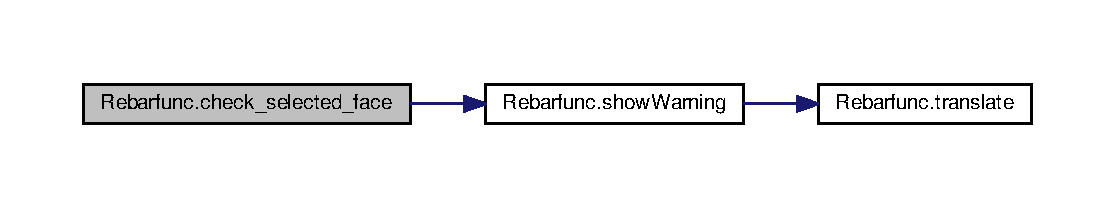
\includegraphics[width=350pt]{namespaceRebarfunc_adae2713855a7e1b4bda04081ae671542_cgraph}
\end{center}
\end{figure}




Here is the caller graph for this function\+:\nopagebreak
\begin{figure}[H]
\begin{center}
\leavevmode
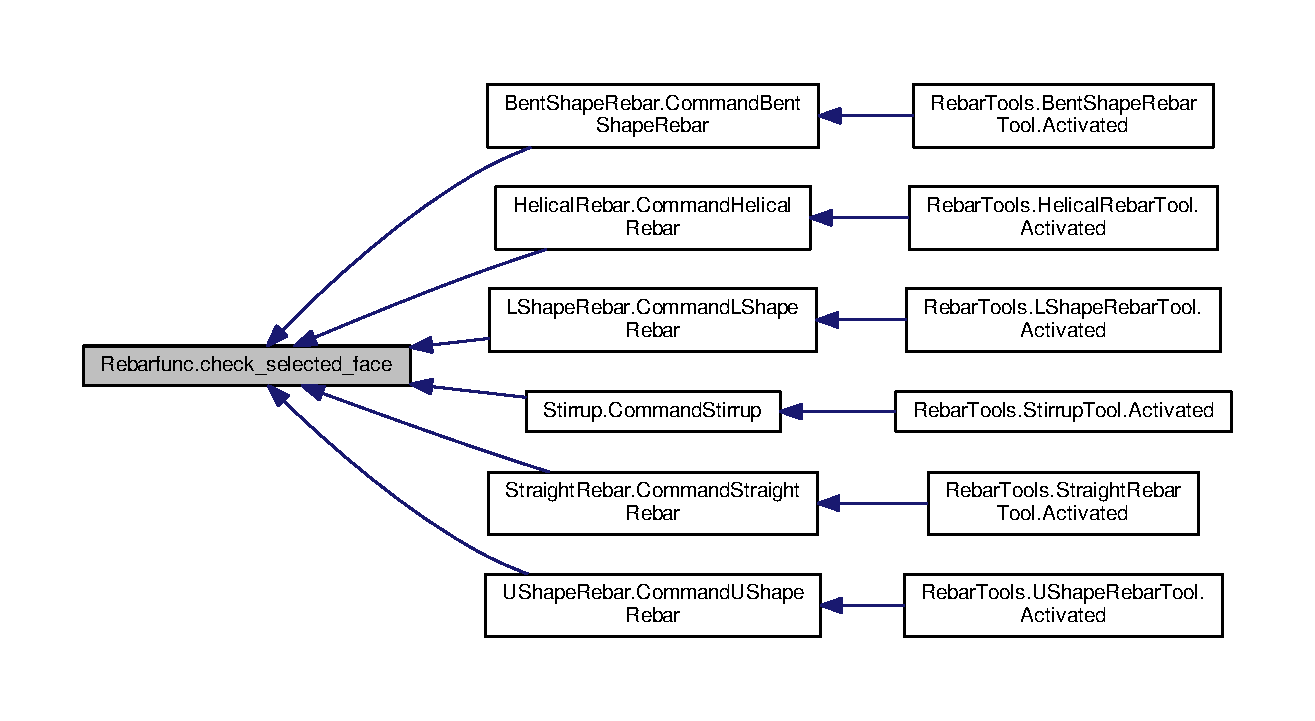
\includegraphics[width=350pt]{namespaceRebarfunc_adae2713855a7e1b4bda04081ae671542_icgraph}
\end{center}
\end{figure}


\index{Rebarfunc@{Rebarfunc}!check\+Rectangle@{check\+Rectangle}}
\index{check\+Rectangle@{check\+Rectangle}!Rebarfunc@{Rebarfunc}}
\subsubsection[{\texorpdfstring{check\+Rectangle(edges)}{checkRectangle(edges)}}]{\setlength{\rightskip}{0pt plus 5cm}def Rebarfunc.\+check\+Rectangle (
\begin{DoxyParamCaption}
\item[{}]{edges}
\end{DoxyParamCaption}
)}\hypertarget{namespaceRebarfunc_a24ab60160ea54e86c0ce1b727621bf71}{}\label{namespaceRebarfunc_a24ab60160ea54e86c0ce1b727621bf71}
\begin{DoxyVerb}checkRectangle(edges=[]): This function checks whether the given form rectangle
    or not. It will return True when edges form rectangular shape or return False
    when edges not form a rectangular.\end{DoxyVerb}
 

Definition at line \hyperlink{Rebarfunc_8py_source_l00046}{46} of file \hyperlink{Rebarfunc_8py_source}{Rebarfunc.\+py}.


\begin{DoxyCode}
\hypertarget{namespaceRebarfunc.tex_l00046}{}\hyperlink{namespaceRebarfunc_a24ab60160ea54e86c0ce1b727621bf71}{00046} \textcolor{keyword}{def }\hyperlink{namespaceRebarfunc_a24ab60160ea54e86c0ce1b727621bf71}{checkRectangle}(edges):
00047     \textcolor{stringliteral}{""" checkRectangle(edges=[]): This function checks whether the given form rectangle}
00048 \textcolor{stringliteral}{        or not. It will return True when edges form rectangular shape or return False}
00049 \textcolor{stringliteral}{        when edges not form a rectangular."""}
00050     angles = [round(\hyperlink{namespaceRebarfunc_a3c75160aea4e3fd67b08c557e53a6910}{getEdgesAngle}(edges[0], edges[1])), round(
      \hyperlink{namespaceRebarfunc_a3c75160aea4e3fd67b08c557e53a6910}{getEdgesAngle}(edges[0], edges[2])),
00051             round(\hyperlink{namespaceRebarfunc_a3c75160aea4e3fd67b08c557e53a6910}{getEdgesAngle}(edges[0], edges[3]))]
00052     \textcolor{keywordflow}{if} angles.count(90) == 2 \textcolor{keywordflow}{and} (angles.count(180) == 1 \textcolor{keywordflow}{or} angles.count(0) == 1):
00053         \textcolor{keywordflow}{return} \textcolor{keyword}{True}
00054     \textcolor{keywordflow}{else}:
00055         \textcolor{keywordflow}{return} \textcolor{keyword}{False}
00056 
\end{DoxyCode}


Here is the call graph for this function\+:\nopagebreak
\begin{figure}[H]
\begin{center}
\leavevmode
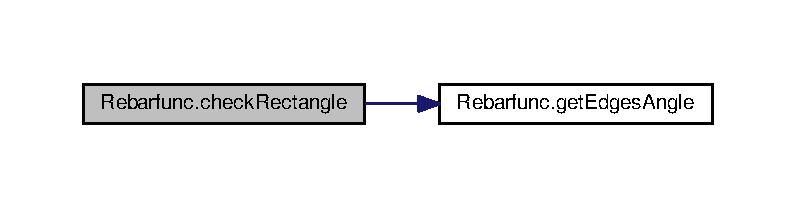
\includegraphics[width=350pt]{namespaceRebarfunc_a24ab60160ea54e86c0ce1b727621bf71_cgraph}
\end{center}
\end{figure}




Here is the caller graph for this function\+:\nopagebreak
\begin{figure}[H]
\begin{center}
\leavevmode
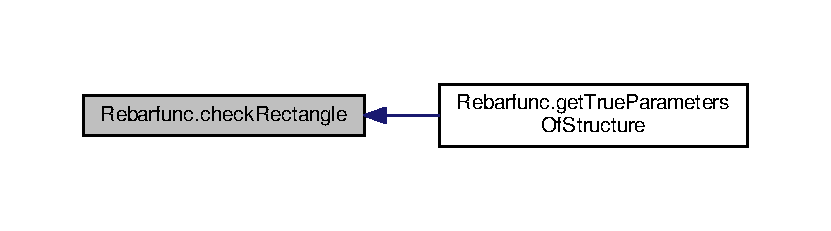
\includegraphics[width=350pt]{namespaceRebarfunc_a24ab60160ea54e86c0ce1b727621bf71_icgraph}
\end{center}
\end{figure}


\index{Rebarfunc@{Rebarfunc}!extended\+Tangent\+Length@{extended\+Tangent\+Length}}
\index{extended\+Tangent\+Length@{extended\+Tangent\+Length}!Rebarfunc@{Rebarfunc}}
\subsubsection[{\texorpdfstring{extended\+Tangent\+Length(rounding, diameter, angle)}{extendedTangentLength(rounding, diameter, angle)}}]{\setlength{\rightskip}{0pt plus 5cm}def Rebarfunc.\+extended\+Tangent\+Length (
\begin{DoxyParamCaption}
\item[{}]{rounding, }
\item[{}]{diameter, }
\item[{}]{angle}
\end{DoxyParamCaption}
)}\hypertarget{namespaceRebarfunc_ab5637ab0a8e202409ee8657d39ca87a0}{}\label{namespaceRebarfunc_ab5637ab0a8e202409ee8657d39ca87a0}
\begin{DoxyVerb}extendedTangentLength(rounding, diameter, angle): Get a extended
length of rounding at the end of Stirrup for bent.\end{DoxyVerb}
 

Definition at line \hyperlink{Rebarfunc_8py_source_l00243}{243} of file \hyperlink{Rebarfunc_8py_source}{Rebarfunc.\+py}.


\begin{DoxyCode}
\hypertarget{namespaceRebarfunc.tex_l00243}{}\hyperlink{namespaceRebarfunc_ab5637ab0a8e202409ee8657d39ca87a0}{00243} \textcolor{keyword}{def }\hyperlink{namespaceRebarfunc_ab5637ab0a8e202409ee8657d39ca87a0}{extendedTangentLength}(rounding, diameter, angle):
00244     \textcolor{stringliteral}{""" extendedTangentLength(rounding, diameter, angle): Get a extended}
00245 \textcolor{stringliteral}{    length of rounding at the end of Stirrup for bent."""}
00246     radius = rounding * diameter
00247     x1 = radius / math.sin(math.radians(angle))
00248     x2 = radius * math.tan(math.radians(90 - angle))
00249     \textcolor{keywordflow}{return} x1 + x2
00250 
00251 \textcolor{comment}{# -------------------------------------------------------------------------}
00252 \textcolor{comment}{# Warning / Alert functions when user do something wrong.}
00253 \textcolor{comment}{#--------------------------------------------------------------------------}
00254 
\end{DoxyCode}


Here is the caller graph for this function\+:\nopagebreak
\begin{figure}[H]
\begin{center}
\leavevmode
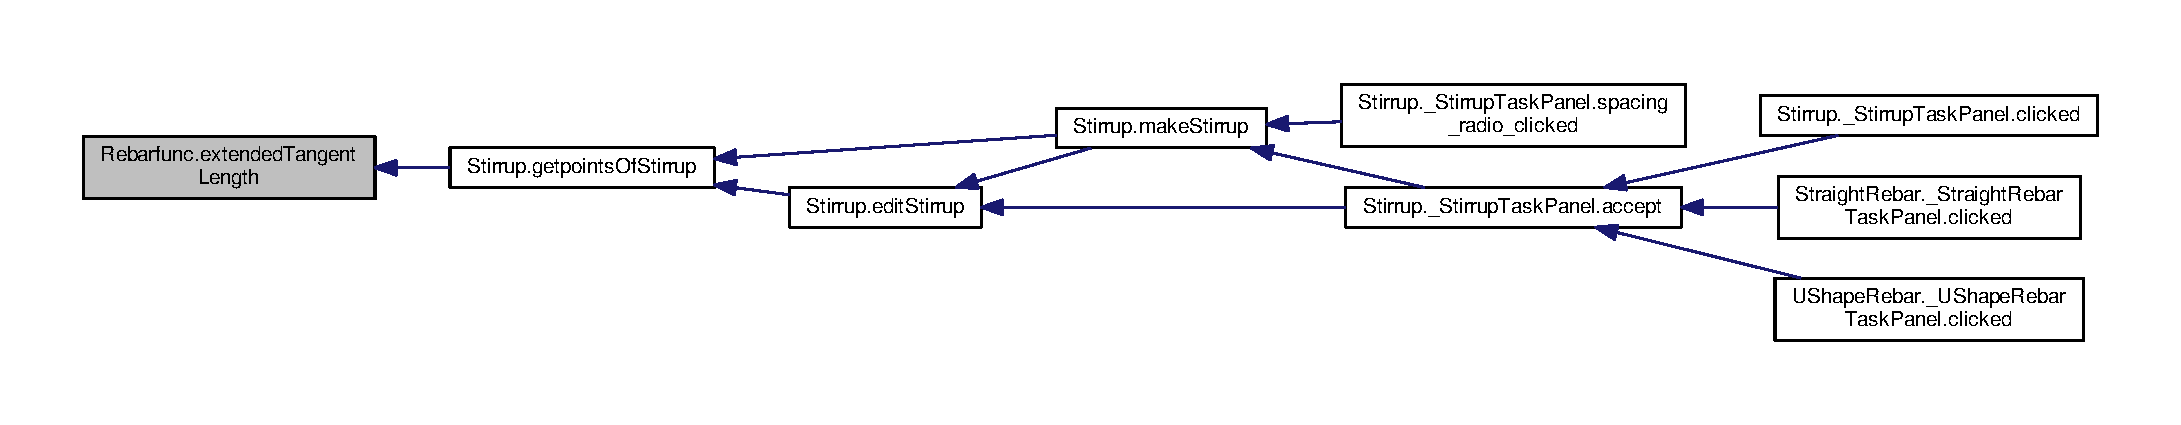
\includegraphics[width=350pt]{namespaceRebarfunc_ab5637ab0a8e202409ee8657d39ca87a0_icgraph}
\end{center}
\end{figure}


\index{Rebarfunc@{Rebarfunc}!extended\+Tangent\+Part\+Length@{extended\+Tangent\+Part\+Length}}
\index{extended\+Tangent\+Part\+Length@{extended\+Tangent\+Part\+Length}!Rebarfunc@{Rebarfunc}}
\subsubsection[{\texorpdfstring{extended\+Tangent\+Part\+Length(rounding, diameter, angle)}{extendedTangentPartLength(rounding, diameter, angle)}}]{\setlength{\rightskip}{0pt plus 5cm}def Rebarfunc.\+extended\+Tangent\+Part\+Length (
\begin{DoxyParamCaption}
\item[{}]{rounding, }
\item[{}]{diameter, }
\item[{}]{angle}
\end{DoxyParamCaption}
)}\hypertarget{namespaceRebarfunc_aaeecb468e0fcfc5eee69d6a24c5c5aef}{}\label{namespaceRebarfunc_aaeecb468e0fcfc5eee69d6a24c5c5aef}
\begin{DoxyVerb}extendedTangentPartLength(rounding, diameter, angle): Get a extended
length of rounding on corners.\end{DoxyVerb}
 

Definition at line \hyperlink{Rebarfunc_8py_source_l00235}{235} of file \hyperlink{Rebarfunc_8py_source}{Rebarfunc.\+py}.


\begin{DoxyCode}
\hypertarget{namespaceRebarfunc.tex_l00235}{}\hyperlink{namespaceRebarfunc_aaeecb468e0fcfc5eee69d6a24c5c5aef}{00235} \textcolor{keyword}{def }\hyperlink{namespaceRebarfunc_aaeecb468e0fcfc5eee69d6a24c5c5aef}{extendedTangentPartLength}(rounding, diameter, angle):
00236     \textcolor{stringliteral}{""" extendedTangentPartLength(rounding, diameter, angle): Get a extended}
00237 \textcolor{stringliteral}{    length of rounding on corners."""}
00238     radius = rounding * diameter
00239     x1 = radius / math.tan(math.radians(angle))
00240     x2 = radius / math.cos(math.radians(90 - angle)) - radius
00241     \textcolor{keywordflow}{return} x1 + x2
00242 
\end{DoxyCode}


Here is the caller graph for this function\+:\nopagebreak
\begin{figure}[H]
\begin{center}
\leavevmode
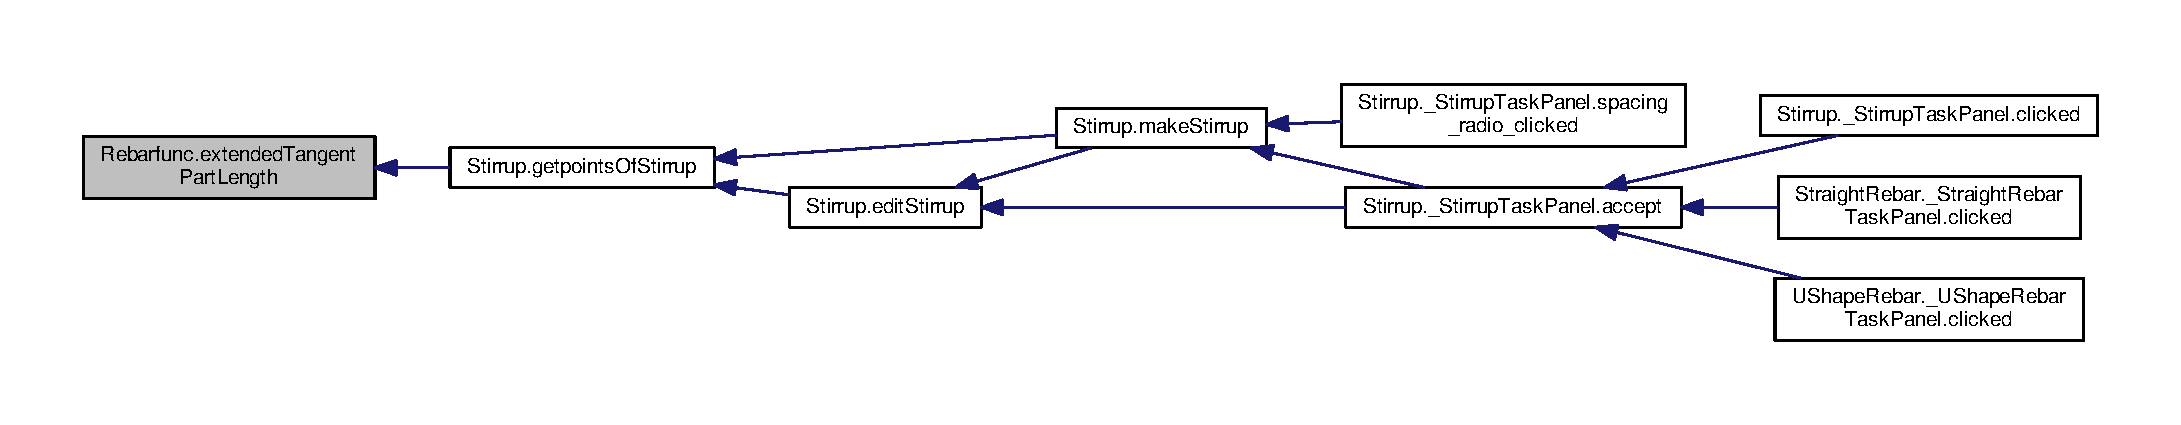
\includegraphics[width=350pt]{namespaceRebarfunc_aaeecb468e0fcfc5eee69d6a24c5c5aef_icgraph}
\end{center}
\end{figure}


\index{Rebarfunc@{Rebarfunc}!facenormal\+Direction@{facenormal\+Direction}}
\index{facenormal\+Direction@{facenormal\+Direction}!Rebarfunc@{Rebarfunc}}
\subsubsection[{\texorpdfstring{facenormal\+Direction(structure=\+None, facename=\+None)}{facenormalDirection(structure=None, facename=None)}}]{\setlength{\rightskip}{0pt plus 5cm}def Rebarfunc.\+facenormal\+Direction (
\begin{DoxyParamCaption}
\item[{}]{structure = {\ttfamily None}, }
\item[{}]{facename = {\ttfamily None}}
\end{DoxyParamCaption}
)}\hypertarget{namespaceRebarfunc_a3a8c123c290609baec3a547c20a561b9}{}\label{namespaceRebarfunc_a3a8c123c290609baec3a547c20a561b9}


Definition at line \hyperlink{Rebarfunc_8py_source_l00081}{81} of file \hyperlink{Rebarfunc_8py_source}{Rebarfunc.\+py}.


\begin{DoxyCode}
\hypertarget{namespaceRebarfunc.tex_l00081}{}\hyperlink{namespaceRebarfunc_a3a8c123c290609baec3a547c20a561b9}{00081} \textcolor{keyword}{def }\hyperlink{namespaceRebarfunc_a3a8c123c290609baec3a547c20a561b9}{facenormalDirection}(structure = None, facename = None):
00082     \textcolor{keywordflow}{if} \textcolor{keywordflow}{not} structure \textcolor{keywordflow}{and} \textcolor{keywordflow}{not} facename:
00083         selected\_obj = FreeCADGui.Selection.getSelectionEx()[0]
00084         structure = selected\_obj.Object
00085         facename = selected\_obj.SubElementNames[0]
00086     face = structure.Shape.Faces[\hyperlink{namespaceRebarfunc_a3885b3b63e3a41508ac79bc7550cf301}{getFaceNumber}(facename) - 1]
00087     normal = face.normalAt(0,0)
00088     normal = face.Placement.Rotation.inverted().multVec(normal)
00089     \textcolor{keywordflow}{return} normal
00090 
00091 \textcolor{comment}{# --------------------------------------------------------------------------}
00092 \textcolor{comment}{# Main functions which is use while creating any rebar.}
00093 \textcolor{comment}{# --------------------------------------------------------------------------}
00094 
\end{DoxyCode}


Here is the call graph for this function\+:\nopagebreak
\begin{figure}[H]
\begin{center}
\leavevmode
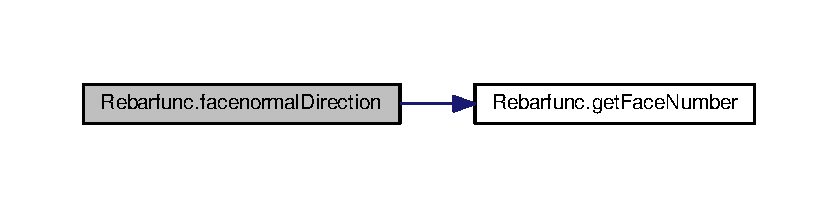
\includegraphics[width=350pt]{namespaceRebarfunc_a3a8c123c290609baec3a547c20a561b9_cgraph}
\end{center}
\end{figure}




Here is the caller graph for this function\+:\nopagebreak
\begin{figure}[H]
\begin{center}
\leavevmode
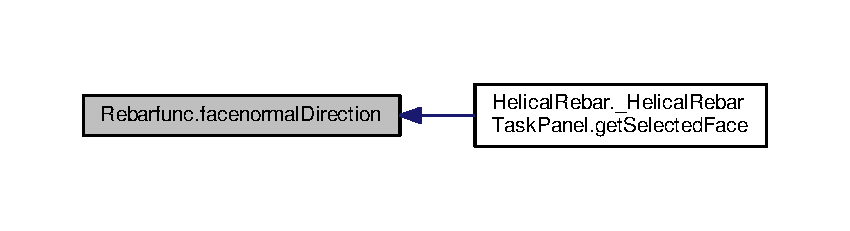
\includegraphics[width=350pt]{namespaceRebarfunc_a3a8c123c290609baec3a547c20a561b9_icgraph}
\end{center}
\end{figure}


\index{Rebarfunc@{Rebarfunc}!get\+Base\+Object@{get\+Base\+Object}}
\index{get\+Base\+Object@{get\+Base\+Object}!Rebarfunc@{Rebarfunc}}
\subsubsection[{\texorpdfstring{get\+Base\+Object(obj)}{getBaseObject(obj)}}]{\setlength{\rightskip}{0pt plus 5cm}def Rebarfunc.\+get\+Base\+Object (
\begin{DoxyParamCaption}
\item[{}]{obj}
\end{DoxyParamCaption}
)}\hypertarget{namespaceRebarfunc_a7169bcadefe75626e6cfb7549b1deb4b}{}\label{namespaceRebarfunc_a7169bcadefe75626e6cfb7549b1deb4b}
\begin{DoxyVerb}getBaseObject(obj): This function will return last base object.\end{DoxyVerb}
 

Definition at line \hyperlink{Rebarfunc_8py_source_l00065}{65} of file \hyperlink{Rebarfunc_8py_source}{Rebarfunc.\+py}.


\begin{DoxyCode}
\hypertarget{namespaceRebarfunc.tex_l00065}{}\hyperlink{namespaceRebarfunc_a7169bcadefe75626e6cfb7549b1deb4b}{00065} \textcolor{keyword}{def }\hyperlink{namespaceRebarfunc_a7169bcadefe75626e6cfb7549b1deb4b}{getBaseObject}(obj):
00066     \textcolor{stringliteral}{""" getBaseObject(obj): This function will return last base object."""}
00067     \textcolor{keywordflow}{if} hasattr(obj, \textcolor{stringliteral}{"Base"}):
00068         \textcolor{keywordflow}{return} \hyperlink{namespaceRebarfunc_a7169bcadefe75626e6cfb7549b1deb4b}{getBaseObject}(obj.Base)
00069     \textcolor{keywordflow}{else}:
00070         \textcolor{keywordflow}{return} obj
00071 
\end{DoxyCode}


Here is the caller graph for this function\+:\nopagebreak
\begin{figure}[H]
\begin{center}
\leavevmode
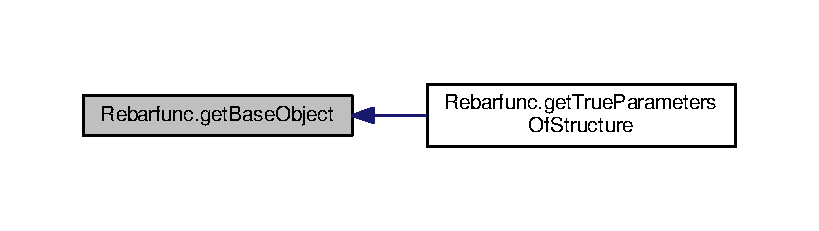
\includegraphics[width=350pt]{namespaceRebarfunc_a7169bcadefe75626e6cfb7549b1deb4b_icgraph}
\end{center}
\end{figure}


\index{Rebarfunc@{Rebarfunc}!get\+Base\+Structural\+Object@{get\+Base\+Structural\+Object}}
\index{get\+Base\+Structural\+Object@{get\+Base\+Structural\+Object}!Rebarfunc@{Rebarfunc}}
\subsubsection[{\texorpdfstring{get\+Base\+Structural\+Object(obj)}{getBaseStructuralObject(obj)}}]{\setlength{\rightskip}{0pt plus 5cm}def Rebarfunc.\+get\+Base\+Structural\+Object (
\begin{DoxyParamCaption}
\item[{}]{obj}
\end{DoxyParamCaption}
)}\hypertarget{namespaceRebarfunc_a20bba2119d962302eada384246cd6270}{}\label{namespaceRebarfunc_a20bba2119d962302eada384246cd6270}
\begin{DoxyVerb}getBaseStructuralObject(obj): This function will return last base
    structural object.\end{DoxyVerb}
 

Definition at line \hyperlink{Rebarfunc_8py_source_l00057}{57} of file \hyperlink{Rebarfunc_8py_source}{Rebarfunc.\+py}.


\begin{DoxyCode}
\hypertarget{namespaceRebarfunc.tex_l00057}{}\hyperlink{namespaceRebarfunc_a20bba2119d962302eada384246cd6270}{00057} \textcolor{keyword}{def }\hyperlink{namespaceRebarfunc_a20bba2119d962302eada384246cd6270}{getBaseStructuralObject}(obj):
00058     \textcolor{stringliteral}{""" getBaseStructuralObject(obj): This function will return last base}
00059 \textcolor{stringliteral}{        structural object."""}
00060     \textcolor{keywordflow}{if} \textcolor{keywordflow}{not} obj.Base:
00061         \textcolor{keywordflow}{return} obj
00062     \textcolor{keywordflow}{else}:
00063         \textcolor{keywordflow}{return} \hyperlink{namespaceRebarfunc_a20bba2119d962302eada384246cd6270}{getBaseStructuralObject}(obj.Base)
00064 
\end{DoxyCode}


Here is the caller graph for this function\+:\nopagebreak
\begin{figure}[H]
\begin{center}
\leavevmode
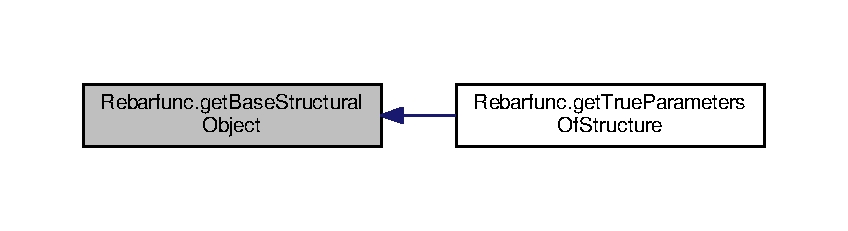
\includegraphics[width=350pt]{namespaceRebarfunc_a20bba2119d962302eada384246cd6270_icgraph}
\end{center}
\end{figure}


\index{Rebarfunc@{Rebarfunc}!get\+Edges\+Angle@{get\+Edges\+Angle}}
\index{get\+Edges\+Angle@{get\+Edges\+Angle}!Rebarfunc@{Rebarfunc}}
\subsubsection[{\texorpdfstring{get\+Edges\+Angle(edge1, edge2)}{getEdgesAngle(edge1, edge2)}}]{\setlength{\rightskip}{0pt plus 5cm}def Rebarfunc.\+get\+Edges\+Angle (
\begin{DoxyParamCaption}
\item[{}]{edge1, }
\item[{}]{edge2}
\end{DoxyParamCaption}
)}\hypertarget{namespaceRebarfunc_a3c75160aea4e3fd67b08c557e53a6910}{}\label{namespaceRebarfunc_a3c75160aea4e3fd67b08c557e53a6910}
\begin{DoxyVerb}getEdgesAngle(edge1, edge2): returns a angle between two edges.\end{DoxyVerb}
 

Definition at line \hyperlink{Rebarfunc_8py_source_l00038}{38} of file \hyperlink{Rebarfunc_8py_source}{Rebarfunc.\+py}.


\begin{DoxyCode}
\hypertarget{namespaceRebarfunc.tex_l00038}{}\hyperlink{namespaceRebarfunc_a3c75160aea4e3fd67b08c557e53a6910}{00038} \textcolor{keyword}{def }\hyperlink{namespaceRebarfunc_a3c75160aea4e3fd67b08c557e53a6910}{getEdgesAngle}(edge1, edge2):
00039     \textcolor{stringliteral}{""" getEdgesAngle(edge1, edge2): returns a angle between two edges."""}
00040     vec1 = vec(edge1)
00041     vec2 = vec(edge2)
00042     angle = vec1.getAngle(vec2)
00043     angle = math.degrees(angle)
00044     \textcolor{keywordflow}{return} angle
00045 
\end{DoxyCode}


Here is the caller graph for this function\+:\nopagebreak
\begin{figure}[H]
\begin{center}
\leavevmode
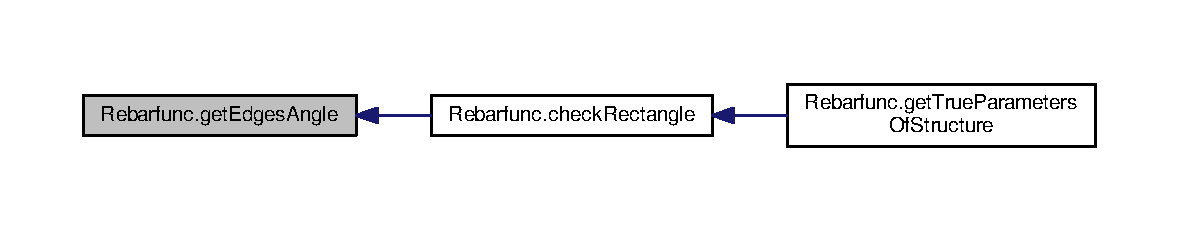
\includegraphics[width=350pt]{namespaceRebarfunc_a3c75160aea4e3fd67b08c557e53a6910_icgraph}
\end{center}
\end{figure}


\index{Rebarfunc@{Rebarfunc}!get\+Face\+Number@{get\+Face\+Number}}
\index{get\+Face\+Number@{get\+Face\+Number}!Rebarfunc@{Rebarfunc}}
\subsubsection[{\texorpdfstring{get\+Face\+Number(s)}{getFaceNumber(s)}}]{\setlength{\rightskip}{0pt plus 5cm}def Rebarfunc.\+get\+Face\+Number (
\begin{DoxyParamCaption}
\item[{}]{s}
\end{DoxyParamCaption}
)}\hypertarget{namespaceRebarfunc_a3885b3b63e3a41508ac79bc7550cf301}{}\label{namespaceRebarfunc_a3885b3b63e3a41508ac79bc7550cf301}
\begin{DoxyVerb}getFaceNumber(facename): This will return a face number from face name.
For eg.:
    Input: "Face12"
    Output: 12\end{DoxyVerb}
 

Definition at line \hyperlink{Rebarfunc_8py_source_l00072}{72} of file \hyperlink{Rebarfunc_8py_source}{Rebarfunc.\+py}.


\begin{DoxyCode}
\hypertarget{namespaceRebarfunc.tex_l00072}{}\hyperlink{namespaceRebarfunc_a3885b3b63e3a41508ac79bc7550cf301}{00072} \textcolor{keyword}{def }\hyperlink{namespaceRebarfunc_a3885b3b63e3a41508ac79bc7550cf301}{getFaceNumber}(s):
00073     \textcolor{stringliteral}{""" getFaceNumber(facename): This will return a face number from face name.}
00074 \textcolor{stringliteral}{    For eg.:}
00075 \textcolor{stringliteral}{        Input: "Face12"}
00076 \textcolor{stringliteral}{        Output: 12"""}
00077     head = s.rstrip(\textcolor{stringliteral}{'0123456789'})
00078     tail = s[len(head):]
00079     \textcolor{keywordflow}{return} int(tail)
00080 
\end{DoxyCode}


Here is the caller graph for this function\+:\nopagebreak
\begin{figure}[H]
\begin{center}
\leavevmode
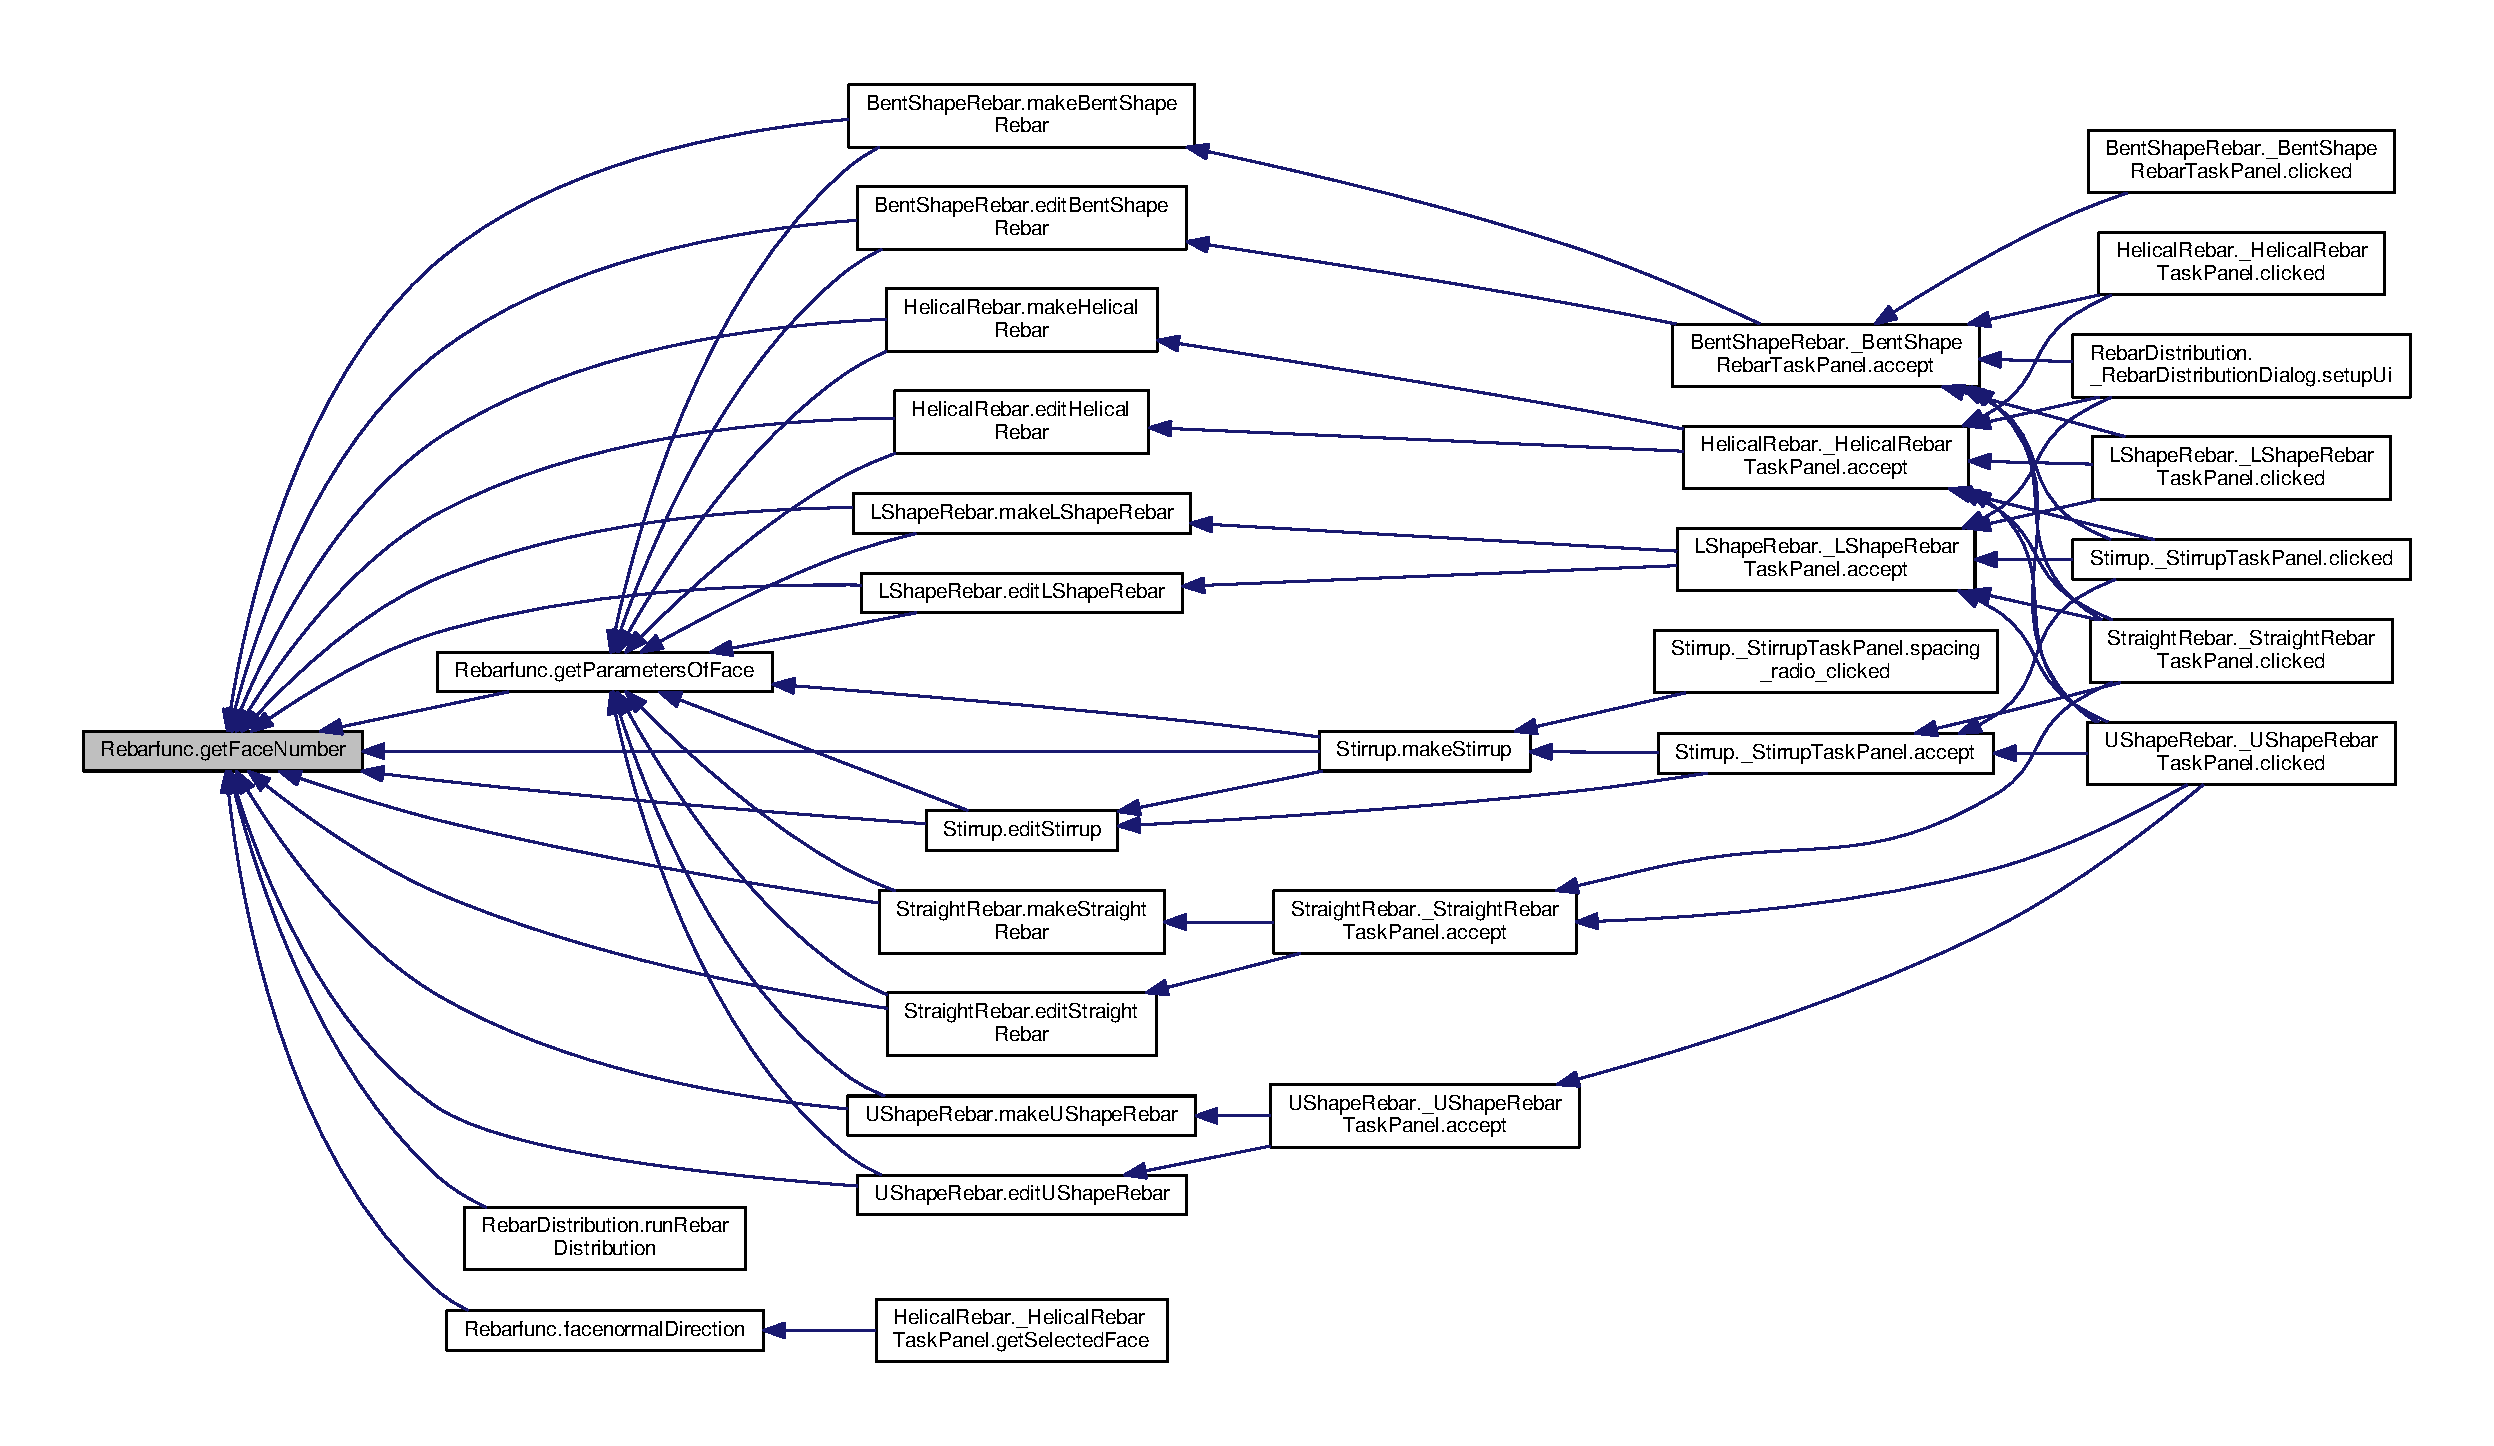
\includegraphics[width=350pt]{namespaceRebarfunc_a3885b3b63e3a41508ac79bc7550cf301_icgraph}
\end{center}
\end{figure}


\index{Rebarfunc@{Rebarfunc}!get\+Parameters\+Of\+Face@{get\+Parameters\+Of\+Face}}
\index{get\+Parameters\+Of\+Face@{get\+Parameters\+Of\+Face}!Rebarfunc@{Rebarfunc}}
\subsubsection[{\texorpdfstring{get\+Parameters\+Of\+Face(structure, facename, sketch=\+True)}{getParametersOfFace(structure, facename, sketch=True)}}]{\setlength{\rightskip}{0pt plus 5cm}def Rebarfunc.\+get\+Parameters\+Of\+Face (
\begin{DoxyParamCaption}
\item[{}]{structure, }
\item[{}]{facename, }
\item[{}]{sketch = {\ttfamily True}}
\end{DoxyParamCaption}
)}\hypertarget{namespaceRebarfunc_a92122b3d7cedd3d47bb63380a5ac4d08}{}\label{namespaceRebarfunc_a92122b3d7cedd3d47bb63380a5ac4d08}
\begin{DoxyVerb}getParametersOfFace(structure, facename, sketch = True): This function will return
length, width and points of center of mass of a given face according to the sketch
value in the form of list.

For eg.:
Case 1: When sketch is True: We use True when we want to create rebars from sketch
    (planar rebars) and the sketch is strictly based on 2D so we neglected the normal
    axis of the face.
    Output: [(FaceLength, FaceWidth), (CenterOfMassX, CenterOfMassY)]

Case 2: When sketch is False: When we want to create non-planar rebars(like stirrup)
    or we want to create rebar from a wire. Also for creating rebar from wire
    we will require three coordinates (x, y, z).
    Output: [(FaceLength, FaceWidth), (CenterOfMassX, CenterOfMassY, CenterOfMassZ)]\end{DoxyVerb}
 

Definition at line \hyperlink{Rebarfunc_8py_source_l00126}{126} of file \hyperlink{Rebarfunc_8py_source}{Rebarfunc.\+py}.


\begin{DoxyCode}
\hypertarget{namespaceRebarfunc.tex_l00126}{}\hyperlink{namespaceRebarfunc_a92122b3d7cedd3d47bb63380a5ac4d08}{00126} \textcolor{keyword}{def }\hyperlink{namespaceRebarfunc_a92122b3d7cedd3d47bb63380a5ac4d08}{getParametersOfFace}(structure, facename, sketch = True):
00127     \textcolor{stringliteral}{""" getParametersOfFace(structure, facename, sketch = True): This function will return}
00128 \textcolor{stringliteral}{    length, width and points of center of mass of a given face according to the sketch}
00129 \textcolor{stringliteral}{    value in the form of list.}
00130 \textcolor{stringliteral}{}
00131 \textcolor{stringliteral}{    For eg.:}
00132 \textcolor{stringliteral}{    Case 1: When sketch is True: We use True when we want to create rebars from sketch}
00133 \textcolor{stringliteral}{        (planar rebars) and the sketch is strictly based on 2D so we neglected the normal}
00134 \textcolor{stringliteral}{        axis of the face.}
00135 \textcolor{stringliteral}{        Output: [(FaceLength, FaceWidth), (CenterOfMassX, CenterOfMassY)]}
00136 \textcolor{stringliteral}{}
00137 \textcolor{stringliteral}{    Case 2: When sketch is False: When we want to create non-planar rebars(like stirrup)}
00138 \textcolor{stringliteral}{        or we want to create rebar from a wire. Also for creating rebar from wire}
00139 \textcolor{stringliteral}{        we will require three coordinates (x, y, z).}
00140 \textcolor{stringliteral}{        Output: [(FaceLength, FaceWidth), (CenterOfMassX, CenterOfMassY, CenterOfMassZ)]"""}
00141     face = structure.Shape.Faces[\hyperlink{namespaceRebarfunc_a3885b3b63e3a41508ac79bc7550cf301}{getFaceNumber}(facename) - 1]
00142     center\_of\_mass = face.CenterOfMass
00143     \textcolor{comment}{#center\_of\_mass = center\_of\_mass.sub(getBaseStructuralObject(structure).Placement.Base)}
00144     center\_of\_mass = center\_of\_mass.sub(structure.Placement.Base)
00145     Edges = []
00146     facePRM = []
00147     \textcolor{comment}{# When structure is cubic. It support all structure is derived from}
00148     \textcolor{comment}{# any other object (like a sketch, wire etc).}
00149     \textcolor{keywordflow}{if} isCubic(structure.Shape):
00150         \textcolor{keywordflow}{print} 423
00151         \textcolor{keywordflow}{for} edge \textcolor{keywordflow}{in} face.Edges:
00152             \textcolor{keywordflow}{if} \textcolor{keywordflow}{not} Edges:
00153                 Edges.append(edge)
00154             \textcolor{keywordflow}{else}:
00155                 \textcolor{comment}{# Checks whether similar edges is already present in Edges list}
00156                 \textcolor{comment}{# or not.}
00157                 \textcolor{keywordflow}{if} round((vec(edge)).Length) \textcolor{keywordflow}{not} \textcolor{keywordflow}{in} [round((vec(x)).Length) \textcolor{keywordflow}{for} x \textcolor{keywordflow}{in} Edges]:
00158                     Edges.append(edge)
00159         \textcolor{keywordflow}{if} len(Edges) == 1:
00160             Edges.append(edge)
00161         \textcolor{comment}{# facePRM holds length of a edges.}
00162         facePRM = [(vec(edge)).Length \textcolor{keywordflow}{for} edge \textcolor{keywordflow}{in} Edges]
00163         \textcolor{comment}{# Find the orientation of the face. Also eliminating normal axes}
00164         \textcolor{comment}{# to the edge/face.}
00165         \textcolor{comment}{# When edge is parallel to x-axis}
00166         \textcolor{keywordflow}{if} round(Edges[0].tangentAt(0)[0]) \textcolor{keywordflow}{in} \{1,-1\}:
00167             x = center\_of\_mass[0]
00168             \textcolor{keywordflow}{if} round(Edges[1].tangentAt(0)[1]) \textcolor{keywordflow}{in} \{1, -1\}:
00169                 y = center\_of\_mass[1]
00170             \textcolor{keywordflow}{else}:
00171                 y = center\_of\_mass[2]
00172         \textcolor{comment}{# When edge is parallel to y-axis}
00173         \textcolor{keywordflow}{elif} round(Edges[0].tangentAt(0)[1]) \textcolor{keywordflow}{in} \{1,-1\}:
00174             x = center\_of\_mass[1]
00175             \textcolor{keywordflow}{if} round(Edges[1].tangentAt(0)[0]) \textcolor{keywordflow}{in} \{1, -1\}:
00176                 \textcolor{comment}{# Change order when edge along x-axis is at second place.}
00177                 facePRM.reverse()
00178                 y = center\_of\_mass[1]
00179             \textcolor{keywordflow}{else}:
00180                 y = center\_of\_mass[2]
00181         \textcolor{keywordflow}{elif} round(Edges[0].tangentAt(0)[2]) \textcolor{keywordflow}{in} \{1,-1\}:
00182             y = center\_of\_mass[2]
00183             \textcolor{keywordflow}{if} round(Edges[1].tangentAt(0)[0]) \textcolor{keywordflow}{in} \{1, -1\}:
00184                 x = center\_of\_mass[0]
00185             \textcolor{keywordflow}{else}:
00186                 x = center\_of\_mass[1]
00187             facePRM.reverse()
00188         facelength = facePRM[0]
00189         facewidth = facePRM[1]
00190     \textcolor{comment}{# When structure is not cubic. For founding parameters of given face}
00191     \textcolor{comment}{# I have used bounding box.}
00192     \textcolor{keywordflow}{else}:
00193         boundbox = face.BoundBox
00194         \textcolor{comment}{# Check that one length of bounding box is zero. Here bounding box}
00195         \textcolor{comment}{# looks like a plane.}
00196         \textcolor{keywordflow}{if} 0 \textcolor{keywordflow}{in} \{round(boundbox.XLength), round(boundbox.YLength), round(boundbox.ZLength)\}:
00197             normal = face.normalAt(0,0)
00198             normal = face.Placement.Rotation.inverted().multVec(normal)
00199             \textcolor{comment}{#print "x: ", boundbox.XLength}
00200             \textcolor{comment}{#print "y: ", boundbox.YLength}
00201             \textcolor{comment}{#print "z: ", boundbox.ZLength}
00202             \textcolor{comment}{# Set length and width of user selected face of structural element}
00203             flag = \textcolor{keyword}{True}
00204             \textcolor{comment}{# FIXME: Improve below logic.}
00205             \textcolor{keywordflow}{for} i \textcolor{keywordflow}{in} range(len(normal)):
00206                 \textcolor{keywordflow}{if} round(normal[i]) == 0:
00207                     \textcolor{keywordflow}{if} flag \textcolor{keywordflow}{and} i == 0:
00208                         x = center\_of\_mass[i]
00209                         facelength =  boundbox.XLength
00210                         flag = \textcolor{keyword}{False}
00211                     \textcolor{keywordflow}{elif} flag \textcolor{keywordflow}{and} i == 1:
00212                         x = center\_of\_mass[i]
00213                         facelength = boundbox.YLength
00214                         flag = \textcolor{keyword}{False}
00215                     \textcolor{keywordflow}{if} i == 1:
00216                         y = center\_of\_mass[i]
00217                         facewidth = boundbox.YLength
00218                     \textcolor{keywordflow}{elif} i == 2:
00219                         y = center\_of\_mass[i]
00220                         facewidth = boundbox.ZLength
00221             \textcolor{comment}{#print [(facelength, facewidth), (x, y)]}
00222     \textcolor{comment}{# Return parameter of the face when rebar is not created from the sketch.}
00223     \textcolor{comment}{# For eg. non-planar rebars like stirrup etc.}
00224     \textcolor{keywordflow}{if} \textcolor{keywordflow}{not} sketch:
00225         center\_of\_mass = face.CenterOfMass
00226         \textcolor{keywordflow}{return} [(facelength, facewidth), center\_of\_mass]
00227     \textcolor{comment}{#TODO: Add support when bounding box have depth. Here bounding box looks}
00228     \textcolor{comment}{# like cuboid. If we given curved face.}
00229     \textcolor{keywordflow}{return} [(facelength, facewidth), (x, y)]
00230 
00231 \textcolor{comment}{# -------------------------------------------------------------------------}
00232 \textcolor{comment}{# Functions which is mainly used while creating stirrup.}
00233 \textcolor{comment}{# -------------------------------------------------------------------------}
00234 
\end{DoxyCode}


Here is the call graph for this function\+:\nopagebreak
\begin{figure}[H]
\begin{center}
\leavevmode
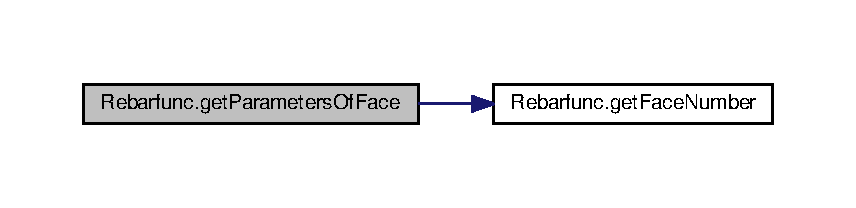
\includegraphics[width=350pt]{namespaceRebarfunc_a92122b3d7cedd3d47bb63380a5ac4d08_cgraph}
\end{center}
\end{figure}




Here is the caller graph for this function\+:\nopagebreak
\begin{figure}[H]
\begin{center}
\leavevmode
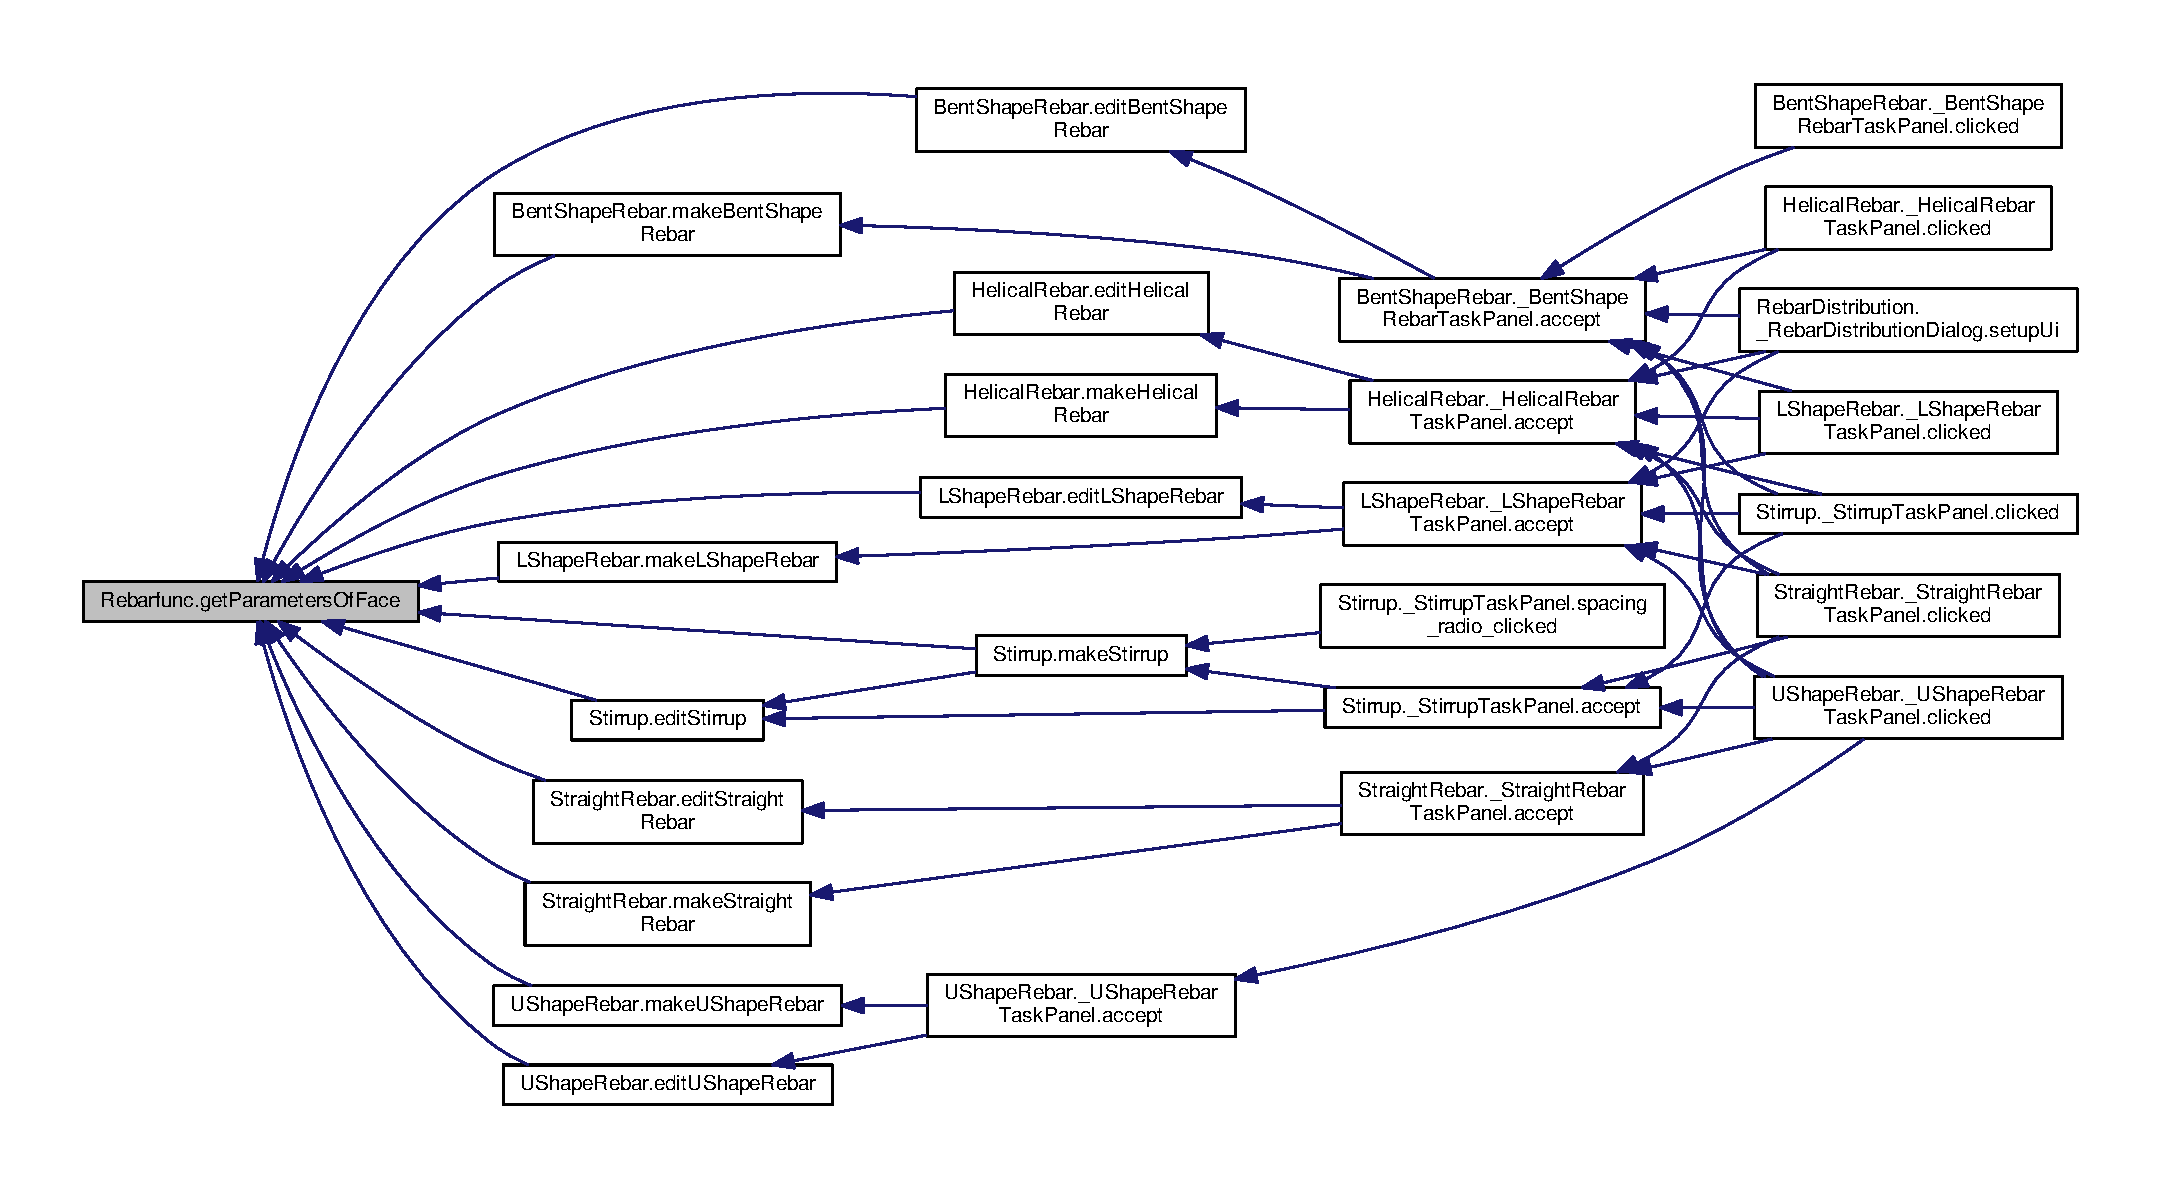
\includegraphics[width=350pt]{namespaceRebarfunc_a92122b3d7cedd3d47bb63380a5ac4d08_icgraph}
\end{center}
\end{figure}


\index{Rebarfunc@{Rebarfunc}!get\+Selected\+Face@{get\+Selected\+Face}}
\index{get\+Selected\+Face@{get\+Selected\+Face}!Rebarfunc@{Rebarfunc}}
\subsubsection[{\texorpdfstring{get\+Selected\+Face(self)}{getSelectedFace(self)}}]{\setlength{\rightskip}{0pt plus 5cm}def Rebarfunc.\+get\+Selected\+Face (
\begin{DoxyParamCaption}
\item[{}]{self}
\end{DoxyParamCaption}
)}\hypertarget{namespaceRebarfunc_a8c003df49ac5f249bd9ea4acfb7d2f8d}{}\label{namespaceRebarfunc_a8c003df49ac5f249bd9ea4acfb7d2f8d}


Definition at line \hyperlink{Rebarfunc_8py_source_l00278}{278} of file \hyperlink{Rebarfunc_8py_source}{Rebarfunc.\+py}.


\begin{DoxyCode}
\hypertarget{namespaceRebarfunc.tex_l00278}{}\hyperlink{namespaceRebarfunc_a8c003df49ac5f249bd9ea4acfb7d2f8d}{00278} \textcolor{keyword}{def }\hyperlink{namespaceRebarfunc_a8c003df49ac5f249bd9ea4acfb7d2f8d}{getSelectedFace}(self):
00279     selected\_objs = FreeCADGui.Selection.getSelectionEx()
00280     \textcolor{keywordflow}{if} selected\_objs:
00281         \textcolor{keywordflow}{if} len(selected\_objs[0].SubObjects) == 1:
00282             \textcolor{keywordflow}{if} \textcolor{stringliteral}{"Face"} \textcolor{keywordflow}{in} selected\_objs[0].SubElementNames[0]:
\hypertarget{namespaceRebarfunc.tex_l00283}{}\hyperlink{namespaceRebarfunc_aca3582a1ad0a9350ca59d02fd3188f80}{00283}                 self.SelectedObj = selected\_objs[0].Object
\hypertarget{namespaceRebarfunc.tex_l00284}{}\hyperlink{namespaceRebarfunc_aa191391fe61fc3fff160a228d66910fc}{00284}                 self.FaceName = selected\_objs[0].SubElementNames[0]
00285                 self.form.PickSelectedFaceLabel.setText(\textcolor{stringliteral}{"Selected face is "} + self.FaceName)
00286             \textcolor{keywordflow}{else}:
00287                 \hyperlink{namespaceRebarfunc_a2278a0602d46a62953af1fcf2e574a94}{showWarning}(\textcolor{stringliteral}{"Select any face of the structural element."})
00288         \textcolor{keywordflow}{else}:
00289             \hyperlink{namespaceRebarfunc_a2278a0602d46a62953af1fcf2e574a94}{showWarning}(\textcolor{stringliteral}{"Select only one face of the structural element."})
00290     \textcolor{keywordflow}{else}:
00291         \hyperlink{namespaceRebarfunc_a2278a0602d46a62953af1fcf2e574a94}{showWarning}(\textcolor{stringliteral}{"Select any face of the structural element."})
00292 
\end{DoxyCode}
\index{Rebarfunc@{Rebarfunc}!get\+True\+Parameters\+Of\+Structure@{get\+True\+Parameters\+Of\+Structure}}
\index{get\+True\+Parameters\+Of\+Structure@{get\+True\+Parameters\+Of\+Structure}!Rebarfunc@{Rebarfunc}}
\subsubsection[{\texorpdfstring{get\+True\+Parameters\+Of\+Structure(obj)}{getTrueParametersOfStructure(obj)}}]{\setlength{\rightskip}{0pt plus 5cm}def Rebarfunc.\+get\+True\+Parameters\+Of\+Structure (
\begin{DoxyParamCaption}
\item[{}]{obj}
\end{DoxyParamCaption}
)}\hypertarget{namespaceRebarfunc_a56b5187c8b2c8bf1b14b4fc88eb6d54c}{}\label{namespaceRebarfunc_a56b5187c8b2c8bf1b14b4fc88eb6d54c}
\begin{DoxyVerb}getTrueParametersOfStructure(obj): This function return actual length,
width and height of the structural element in the form of array like
[Length, Width, Height]\end{DoxyVerb}
 

Definition at line \hyperlink{Rebarfunc_8py_source_l00095}{95} of file \hyperlink{Rebarfunc_8py_source}{Rebarfunc.\+py}.


\begin{DoxyCode}
\hypertarget{namespaceRebarfunc.tex_l00095}{}\hyperlink{namespaceRebarfunc_a56b5187c8b2c8bf1b14b4fc88eb6d54c}{00095} \textcolor{keyword}{def }\hyperlink{namespaceRebarfunc_a56b5187c8b2c8bf1b14b4fc88eb6d54c}{getTrueParametersOfStructure}(obj):
00096     \textcolor{stringliteral}{""" getTrueParametersOfStructure(obj): This function return actual length,}
00097 \textcolor{stringliteral}{    width and height of the structural element in the form of array like}
00098 \textcolor{stringliteral}{    [Length, Width, Height]"""}
00099     baseObject = \hyperlink{namespaceRebarfunc_a7169bcadefe75626e6cfb7549b1deb4b}{getBaseObject}(obj)
00100     \textcolor{comment}{# If selected\_obj is not derived from any base object}
00101     \textcolor{keywordflow}{if} baseObject:
00102         \textcolor{comment}{# If selected\_obj is derived from SketchObject}
00103         \textcolor{keywordflow}{if} baseObject.isDerivedFrom(\textcolor{stringliteral}{"Sketcher::SketchObject"}):
00104             edges = baseObject.Shape.Edges
00105             \textcolor{keywordflow}{if} \hyperlink{namespaceRebarfunc_a24ab60160ea54e86c0ce1b727621bf71}{checkRectangle}(edges):
00106                 \textcolor{keywordflow}{for} edge \textcolor{keywordflow}{in} edges:
00107                     \textcolor{comment}{# Representation vector of edge}
00108                     rep\_vector = edge.Vertexes[1].Point.sub(edge.Vertexes[0].Point)
00109                     rep\_vector\_angle = round(math.degrees(rep\_vector.getAngle(FreeCAD.Vector(1,0,0))))
00110                     \textcolor{keywordflow}{if} rep\_vector\_angle \textcolor{keywordflow}{in} \{0, 180\}:
00111                         length = edge.Length
00112                     \textcolor{keywordflow}{else}:
00113                         width = edge.Length
00114             \textcolor{keywordflow}{else}:
00115                 \textcolor{keywordflow}{return} \textcolor{keywordtype}{None}
00116         \textcolor{keywordflow}{else}:
00117             \textcolor{keywordflow}{return} \textcolor{keywordtype}{None}
00118         height = obj.Height.Value
00119     \textcolor{keywordflow}{else}:
00120         structuralBaseObject = \hyperlink{namespaceRebarfunc_a20bba2119d962302eada384246cd6270}{getBaseStructuralObject}(obj)
00121         length = structuralBaseObject.Length.Value
00122         width = structuralBaseObject.Width.Value
00123         height = structuralBaseObject.Height.Value
00124     \textcolor{keywordflow}{return} [length, width, height]
00125 
\end{DoxyCode}


Here is the call graph for this function\+:\nopagebreak
\begin{figure}[H]
\begin{center}
\leavevmode
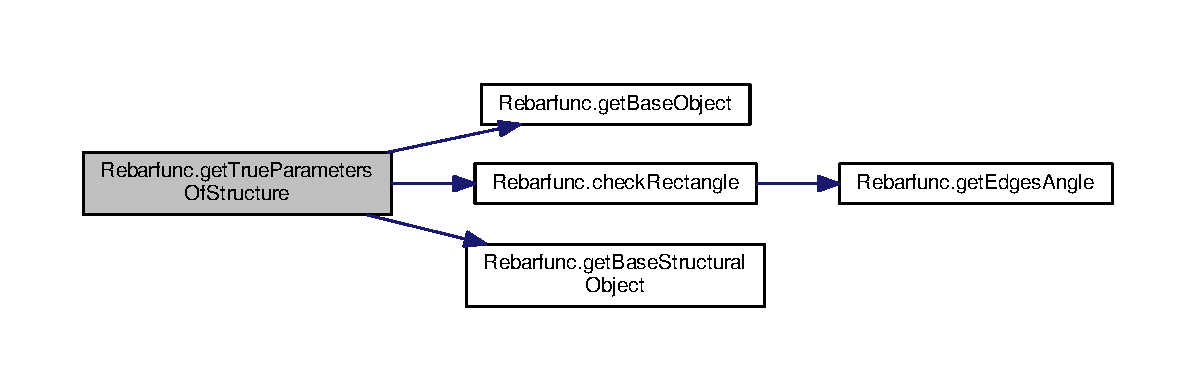
\includegraphics[width=350pt]{namespaceRebarfunc_a56b5187c8b2c8bf1b14b4fc88eb6d54c_cgraph}
\end{center}
\end{figure}


\index{Rebarfunc@{Rebarfunc}!show\+Warning@{show\+Warning}}
\index{show\+Warning@{show\+Warning}!Rebarfunc@{Rebarfunc}}
\subsubsection[{\texorpdfstring{show\+Warning(message)}{showWarning(message)}}]{\setlength{\rightskip}{0pt plus 5cm}def Rebarfunc.\+show\+Warning (
\begin{DoxyParamCaption}
\item[{}]{message}
\end{DoxyParamCaption}
)}\hypertarget{namespaceRebarfunc_a2278a0602d46a62953af1fcf2e574a94}{}\label{namespaceRebarfunc_a2278a0602d46a62953af1fcf2e574a94}
\begin{DoxyVerb}showWarning(message): This function is used to produce warning
message for the user.\end{DoxyVerb}
 

Definition at line \hyperlink{Rebarfunc_8py_source_l00293}{293} of file \hyperlink{Rebarfunc_8py_source}{Rebarfunc.\+py}.


\begin{DoxyCode}
\hypertarget{namespaceRebarfunc.tex_l00293}{}\hyperlink{namespaceRebarfunc_a2278a0602d46a62953af1fcf2e574a94}{00293} \textcolor{keyword}{def }\hyperlink{namespaceRebarfunc_a2278a0602d46a62953af1fcf2e574a94}{showWarning}(message):
00294     \textcolor{stringliteral}{""" showWarning(message): This function is used to produce warning}
00295 \textcolor{stringliteral}{    message for the user."""}
00296     msg = QtGui.QMessageBox()
00297     msg.setIcon(QtGui.QMessageBox.Warning)
00298     msg.setText(\hyperlink{namespaceRebarfunc_a1467a55852e36c36c472e222855bb937}{translate}(\textcolor{stringliteral}{"RebarAddon"}, message))
00299     msg.setStandardButtons(QtGui.QMessageBox.Ok)
00300     msg.exec\_()
00301 
00302 \textcolor{comment}{# Qt tanslation handling}
\end{DoxyCode}


Here is the call graph for this function\+:\nopagebreak
\begin{figure}[H]
\begin{center}
\leavevmode
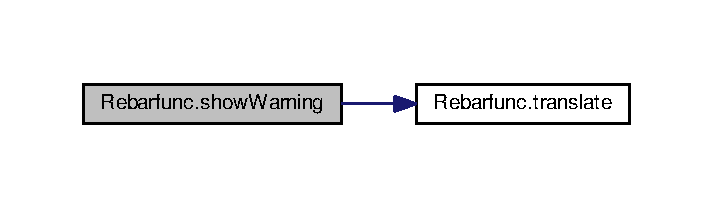
\includegraphics[width=342pt]{namespaceRebarfunc_a2278a0602d46a62953af1fcf2e574a94_cgraph}
\end{center}
\end{figure}




Here is the caller graph for this function\+:\nopagebreak
\begin{figure}[H]
\begin{center}
\leavevmode
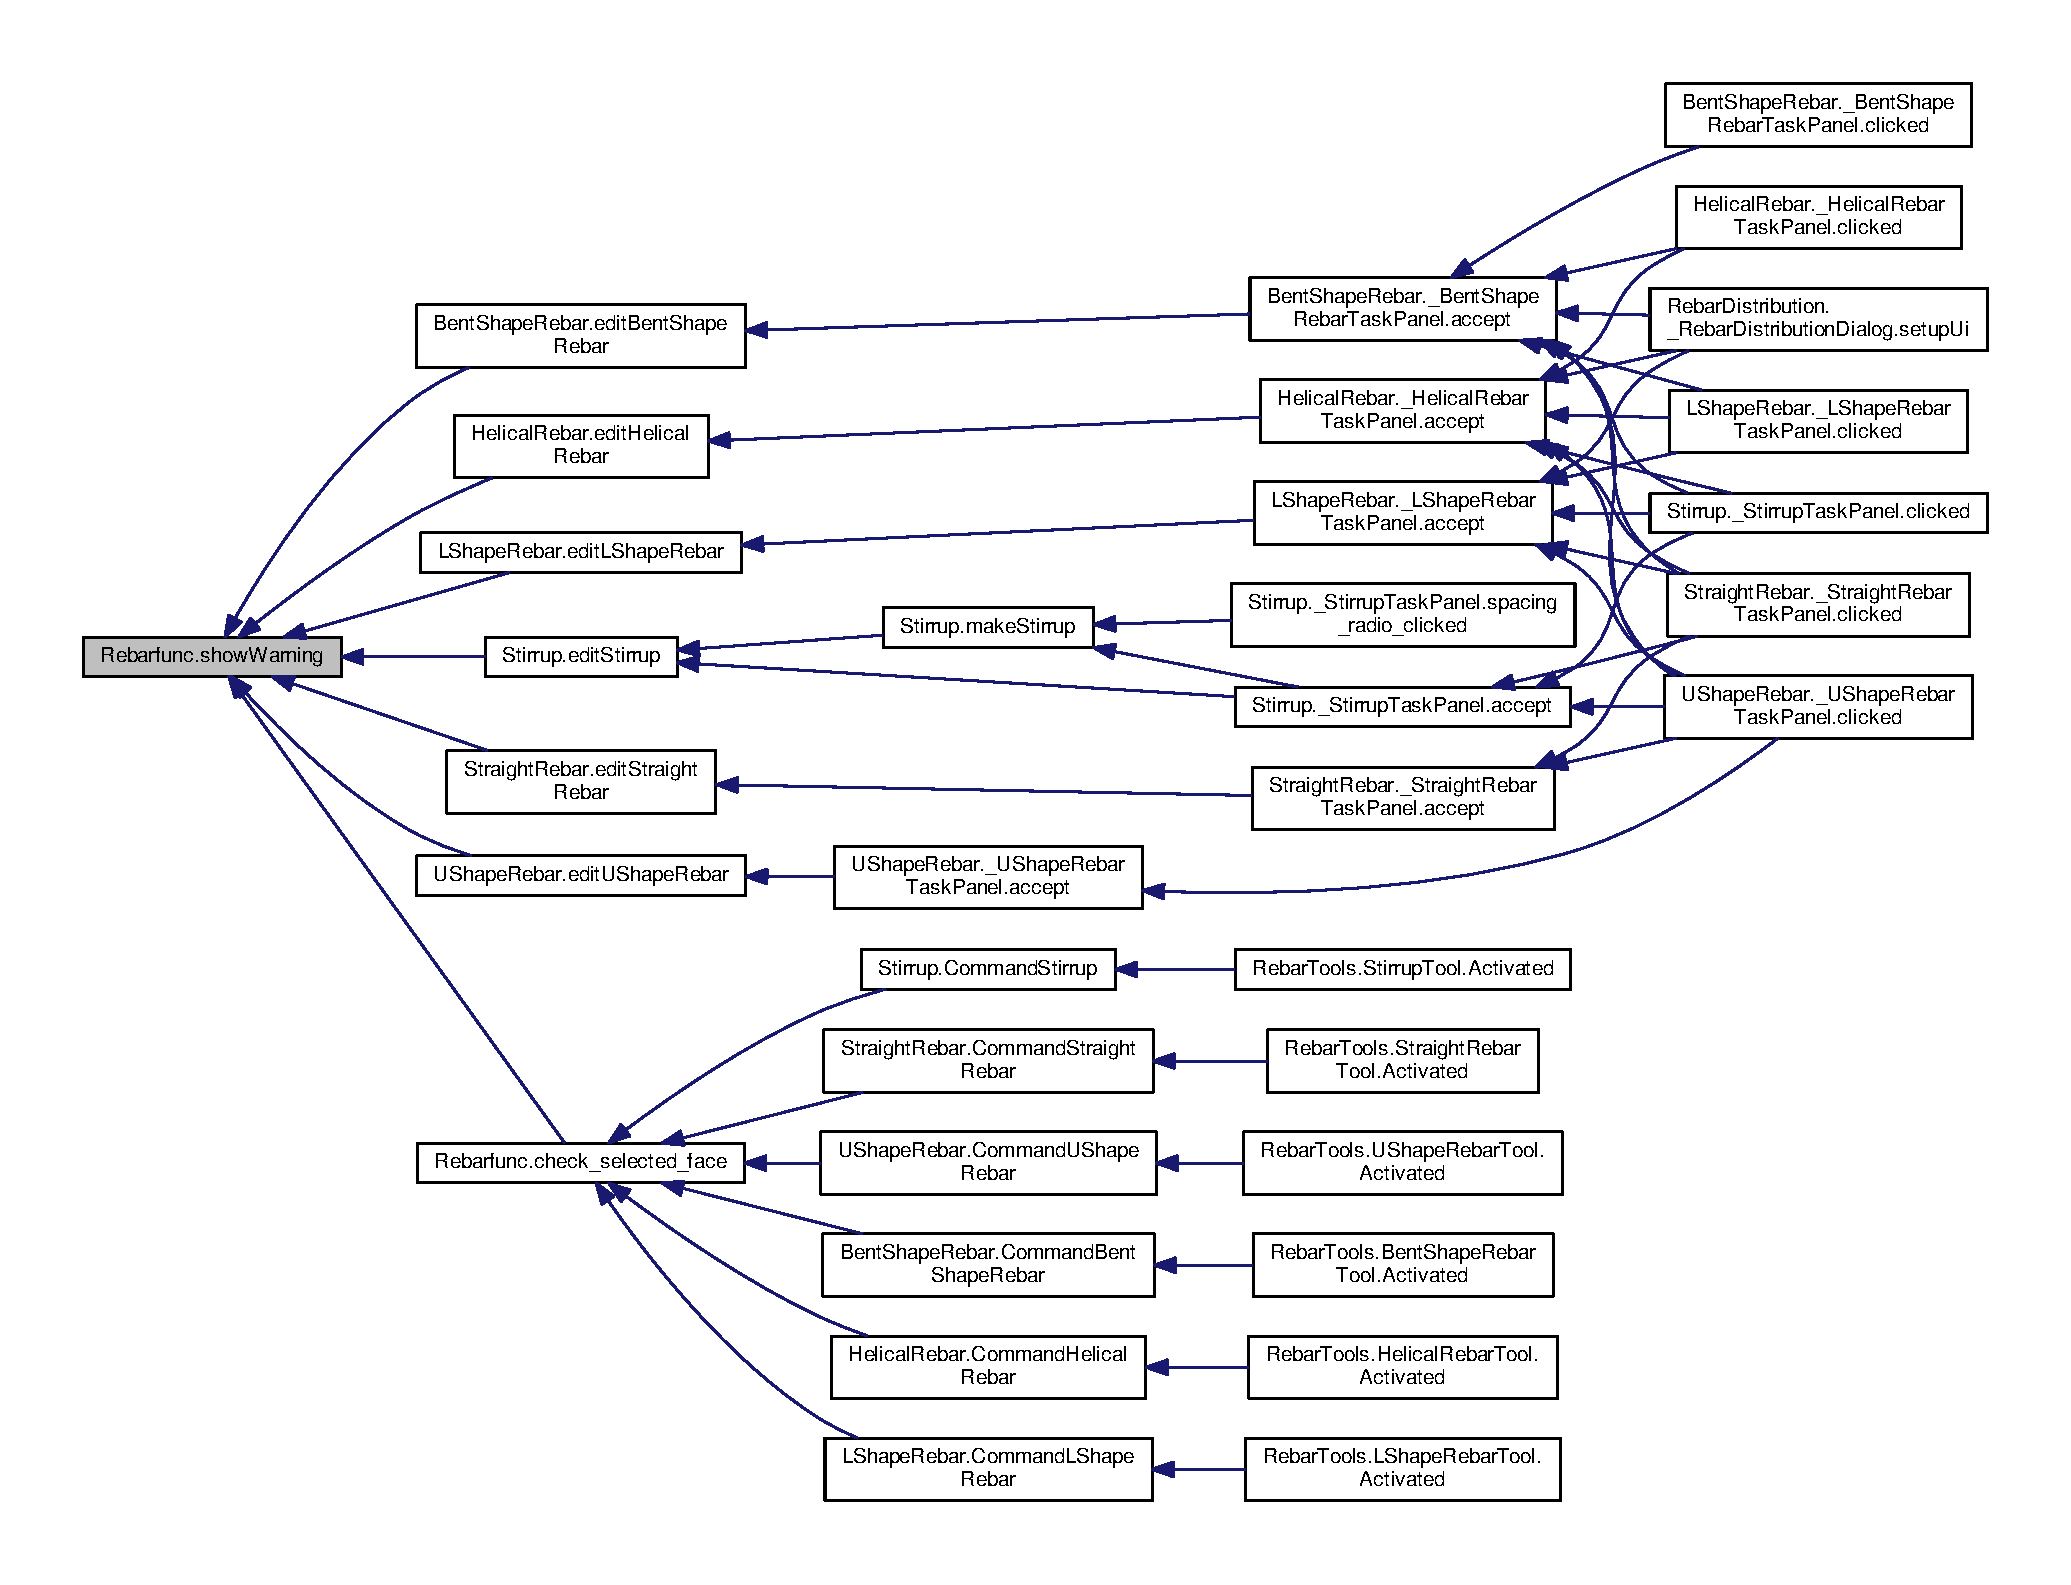
\includegraphics[width=350pt]{namespaceRebarfunc_a2278a0602d46a62953af1fcf2e574a94_icgraph}
\end{center}
\end{figure}


\index{Rebarfunc@{Rebarfunc}!translate@{translate}}
\index{translate@{translate}!Rebarfunc@{Rebarfunc}}
\subsubsection[{\texorpdfstring{translate(context, text, disambig=\+None)}{translate(context, text, disambig=None)}}]{\setlength{\rightskip}{0pt plus 5cm}def Rebarfunc.\+translate (
\begin{DoxyParamCaption}
\item[{}]{context, }
\item[{}]{text, }
\item[{}]{disambig = {\ttfamily None}}
\end{DoxyParamCaption}
)}\hypertarget{namespaceRebarfunc_a1467a55852e36c36c472e222855bb937}{}\label{namespaceRebarfunc_a1467a55852e36c36c472e222855bb937}


Definition at line \hyperlink{Rebarfunc_8py_source_l00303}{303} of file \hyperlink{Rebarfunc_8py_source}{Rebarfunc.\+py}.


\begin{DoxyCode}
\hypertarget{namespaceRebarfunc.tex_l00303}{}\hyperlink{namespaceRebarfunc_a1467a55852e36c36c472e222855bb937}{00303} \textcolor{keyword}{def }\hyperlink{namespaceRebarfunc_a1467a55852e36c36c472e222855bb937}{translate}(context, text, disambig=None):
00304     \textcolor{keywordflow}{return} QtCore.QCoreApplication.translate(context, text, disambig)
00305 \end{DoxyCode}


Here is the caller graph for this function\+:\nopagebreak
\begin{figure}[H]
\begin{center}
\leavevmode
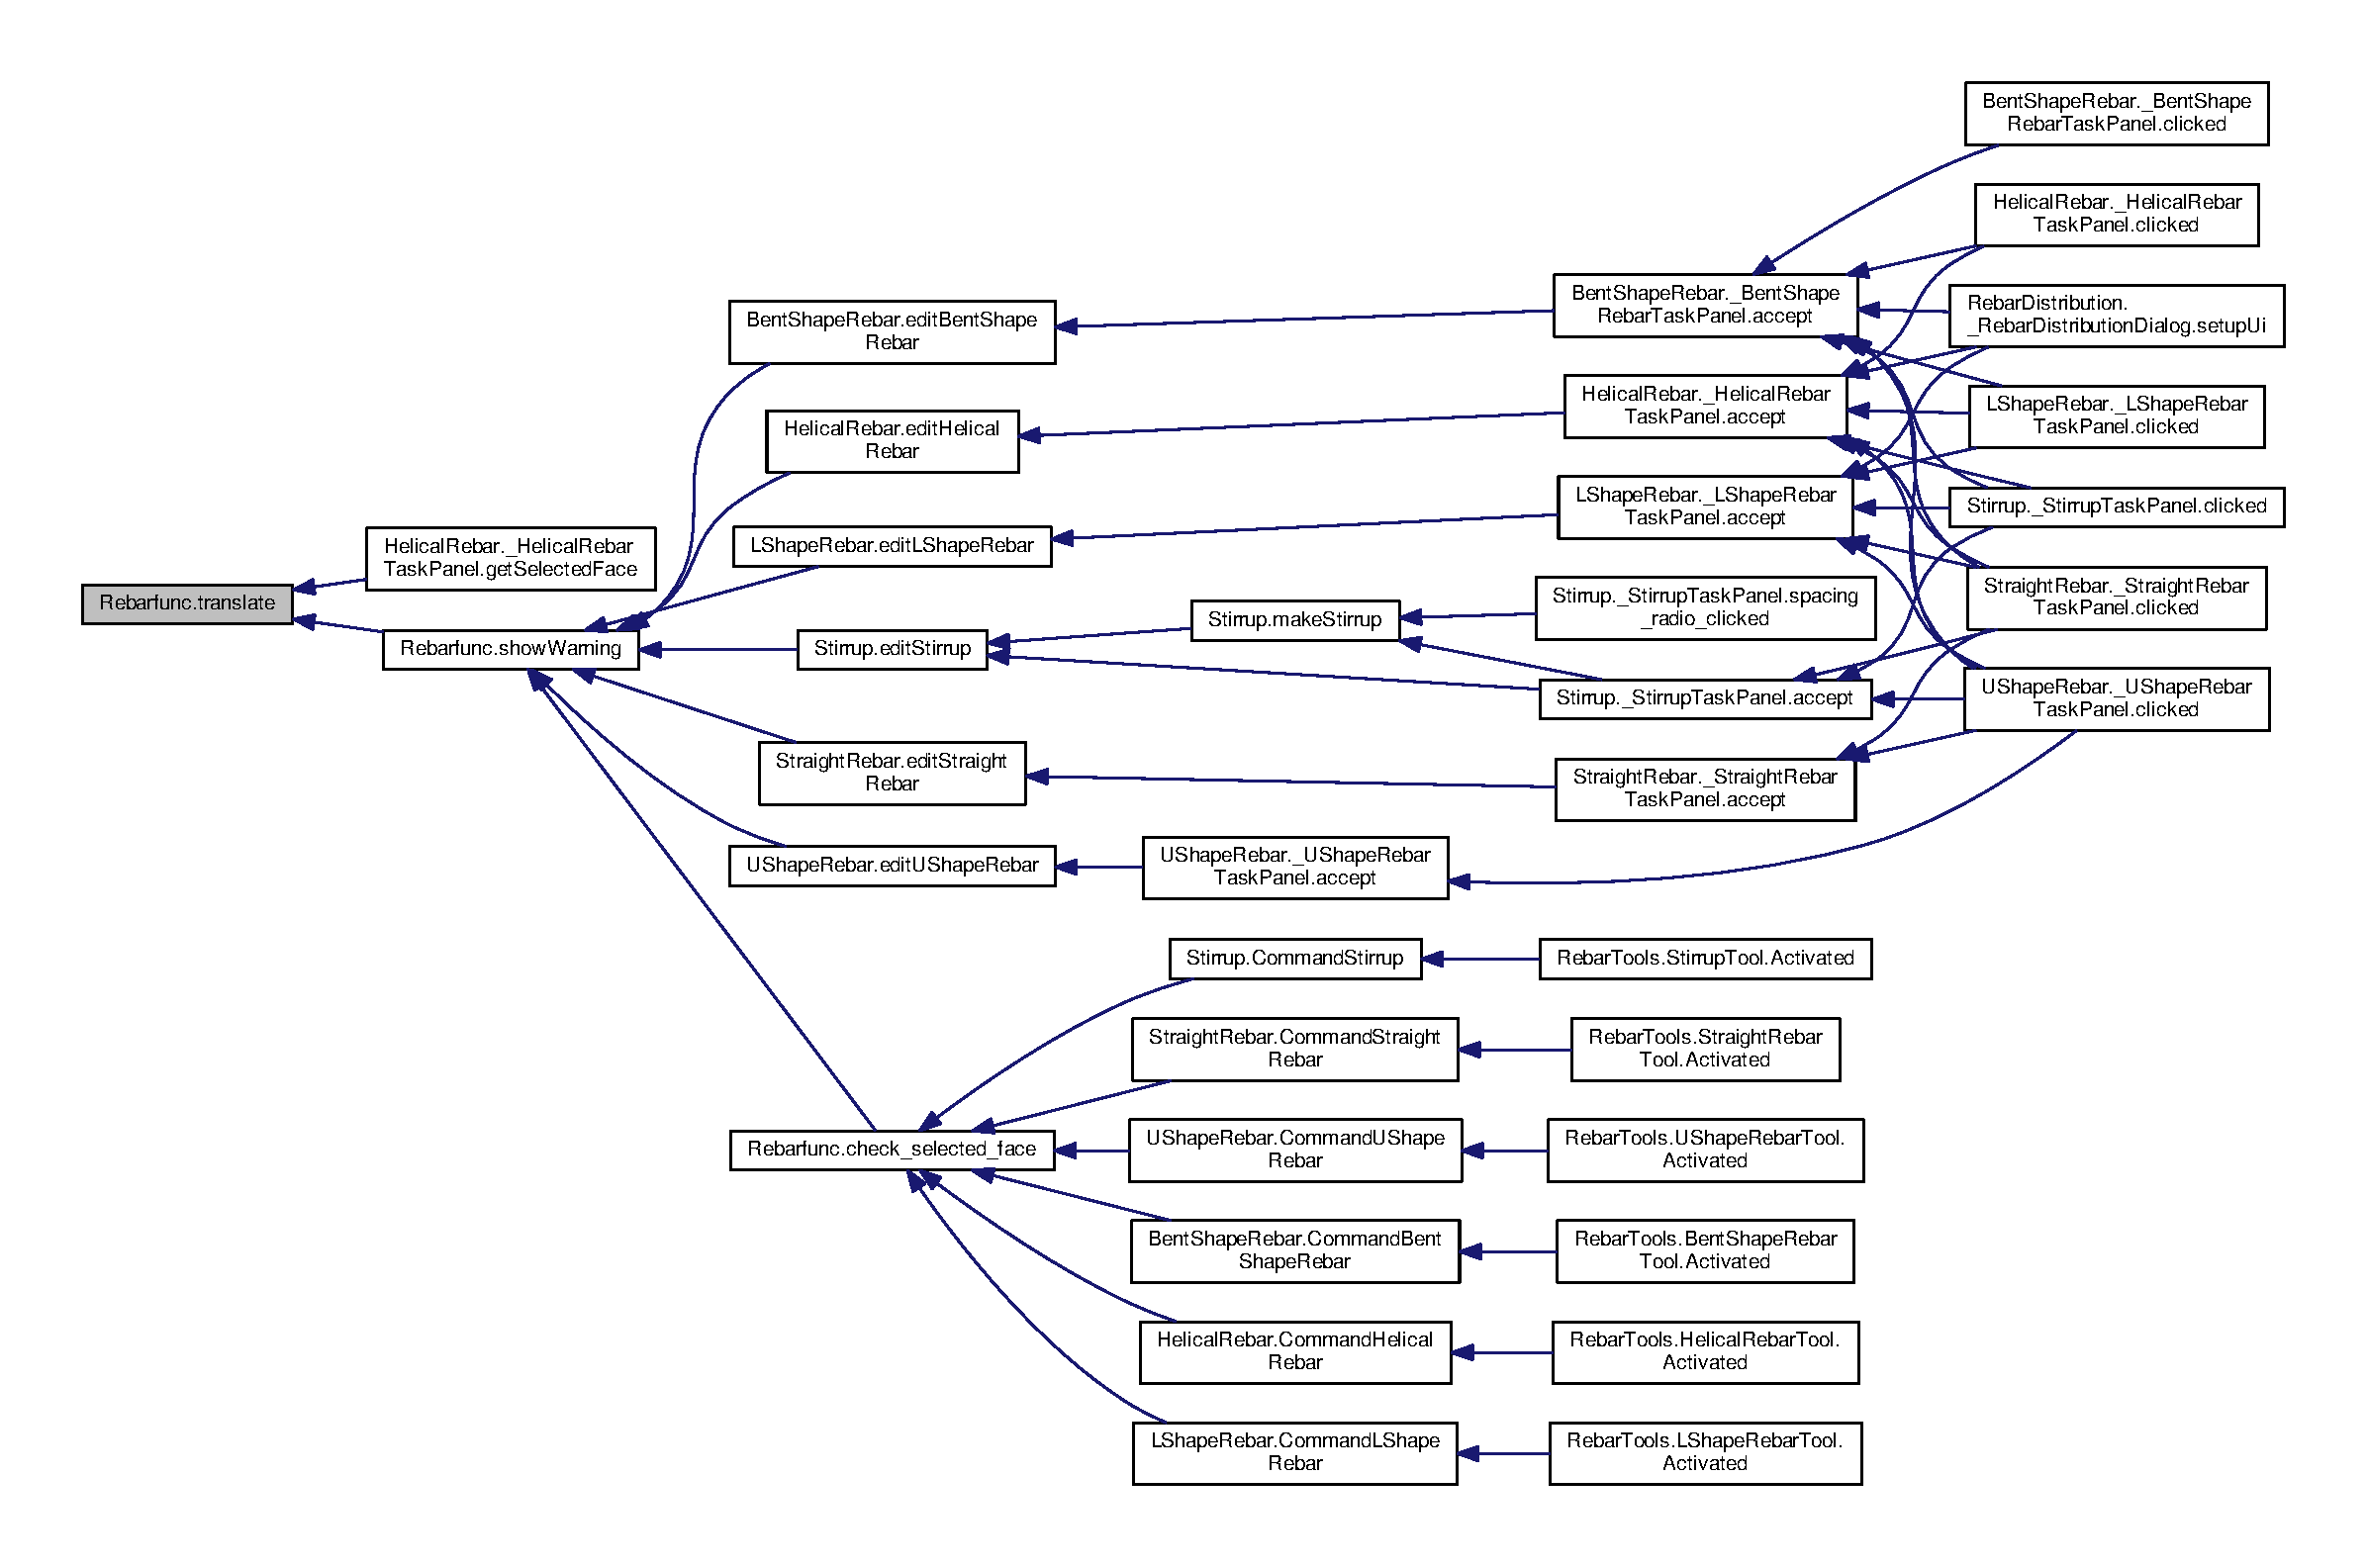
\includegraphics[width=350pt]{namespaceRebarfunc_a1467a55852e36c36c472e222855bb937_icgraph}
\end{center}
\end{figure}




\subsection{Variable Documentation}
\index{Rebarfunc@{Rebarfunc}!\+\_\+\+\_\+author\+\_\+\+\_\+@{\+\_\+\+\_\+author\+\_\+\+\_\+}}
\index{\+\_\+\+\_\+author\+\_\+\+\_\+@{\+\_\+\+\_\+author\+\_\+\+\_\+}!Rebarfunc@{Rebarfunc}}
\subsubsection[{\texorpdfstring{\+\_\+\+\_\+author\+\_\+\+\_\+}{__author__}}]{\setlength{\rightskip}{0pt plus 5cm}string Rebarfunc.\+\_\+\+\_\+author\+\_\+\+\_\+ = \char`\"{}Amritpal Singh\char`\"{}\hspace{0.3cm}{\ttfamily [private]}}\hypertarget{namespaceRebarfunc_aae2a5c81818721137a6cd0f3b66005cb}{}\label{namespaceRebarfunc_aae2a5c81818721137a6cd0f3b66005cb}


Definition at line \hyperlink{Rebarfunc_8py_source_l00025}{25} of file \hyperlink{Rebarfunc_8py_source}{Rebarfunc.\+py}.

\index{Rebarfunc@{Rebarfunc}!\+\_\+\+\_\+title\+\_\+\+\_\+@{\+\_\+\+\_\+title\+\_\+\+\_\+}}
\index{\+\_\+\+\_\+title\+\_\+\+\_\+@{\+\_\+\+\_\+title\+\_\+\+\_\+}!Rebarfunc@{Rebarfunc}}
\subsubsection[{\texorpdfstring{\+\_\+\+\_\+title\+\_\+\+\_\+}{__title__}}]{\setlength{\rightskip}{0pt plus 5cm}string Rebarfunc.\+\_\+\+\_\+title\+\_\+\+\_\+ = \char`\"{}Generic\+Rebar\+Fuctions\char`\"{}\hspace{0.3cm}{\ttfamily [private]}}\hypertarget{namespaceRebarfunc_abd5b4d35a8537923b223274433b692e9}{}\label{namespaceRebarfunc_abd5b4d35a8537923b223274433b692e9}


Definition at line \hyperlink{Rebarfunc_8py_source_l00024}{24} of file \hyperlink{Rebarfunc_8py_source}{Rebarfunc.\+py}.

\index{Rebarfunc@{Rebarfunc}!\+\_\+\+\_\+url\+\_\+\+\_\+@{\+\_\+\+\_\+url\+\_\+\+\_\+}}
\index{\+\_\+\+\_\+url\+\_\+\+\_\+@{\+\_\+\+\_\+url\+\_\+\+\_\+}!Rebarfunc@{Rebarfunc}}
\subsubsection[{\texorpdfstring{\+\_\+\+\_\+url\+\_\+\+\_\+}{__url__}}]{\setlength{\rightskip}{0pt plus 5cm}string Rebarfunc.\+\_\+\+\_\+url\+\_\+\+\_\+ = \char`\"{}https\+://www.\+freecadweb.\+org\char`\"{}\hspace{0.3cm}{\ttfamily [private]}}\hypertarget{namespaceRebarfunc_a11e5d55bb1ddb9fe8f97d06b7916bb22}{}\label{namespaceRebarfunc_a11e5d55bb1ddb9fe8f97d06b7916bb22}


Definition at line \hyperlink{Rebarfunc_8py_source_l00026}{26} of file \hyperlink{Rebarfunc_8py_source}{Rebarfunc.\+py}.

\index{Rebarfunc@{Rebarfunc}!Face\+Name@{Face\+Name}}
\index{Face\+Name@{Face\+Name}!Rebarfunc@{Rebarfunc}}
\subsubsection[{\texorpdfstring{Face\+Name}{FaceName}}]{\setlength{\rightskip}{0pt plus 5cm}Rebarfunc.\+Face\+Name}\hypertarget{namespaceRebarfunc_aa191391fe61fc3fff160a228d66910fc}{}\label{namespaceRebarfunc_aa191391fe61fc3fff160a228d66910fc}


Definition at line \hyperlink{Rebarfunc_8py_source_l00284}{284} of file \hyperlink{Rebarfunc_8py_source}{Rebarfunc.\+py}.

\index{Rebarfunc@{Rebarfunc}!Selected\+Obj@{Selected\+Obj}}
\index{Selected\+Obj@{Selected\+Obj}!Rebarfunc@{Rebarfunc}}
\subsubsection[{\texorpdfstring{Selected\+Obj}{SelectedObj}}]{\setlength{\rightskip}{0pt plus 5cm}Rebarfunc.\+Selected\+Obj}\hypertarget{namespaceRebarfunc_aca3582a1ad0a9350ca59d02fd3188f80}{}\label{namespaceRebarfunc_aca3582a1ad0a9350ca59d02fd3188f80}


Definition at line \hyperlink{Rebarfunc_8py_source_l00283}{283} of file \hyperlink{Rebarfunc_8py_source}{Rebarfunc.\+py}.


\hypertarget{namespaceRebarTools}{}\section{Rebar\+Tools Namespace Reference}
\label{namespaceRebarTools}\index{Rebar\+Tools@{Rebar\+Tools}}
\subsection*{Classes}
\begin{DoxyCompactItemize}
\item 
class \hyperlink{classRebarTools_1_1BentShapeRebarTool}{Bent\+Shape\+Rebar\+Tool}
\item 
class \hyperlink{classRebarTools_1_1HelicalRebarTool}{Helical\+Rebar\+Tool}
\item 
class \hyperlink{classRebarTools_1_1LShapeRebarTool}{L\+Shape\+Rebar\+Tool}
\item 
class \hyperlink{classRebarTools_1_1StirrupTool}{Stirrup\+Tool}
\item 
class \hyperlink{classRebarTools_1_1StraightRebarTool}{Straight\+Rebar\+Tool}
\item 
class \hyperlink{classRebarTools_1_1UShapeRebarTool}{U\+Shape\+Rebar\+Tool}
\end{DoxyCompactItemize}
\subsection*{Variables}
\begin{DoxyCompactItemize}
\item 
string \hyperlink{namespaceRebarTools_a4e380bda06a3907d50e62c4d39b18109}{\+\_\+\+\_\+title\+\_\+\+\_\+} = \char`\"{}Rebar\+Commands\char`\"{}
\item 
string \hyperlink{namespaceRebarTools_a9b758bc71542f069b1d43d0492dfeb35}{\+\_\+\+\_\+author\+\_\+\+\_\+} = \char`\"{}Amritpal Singh\char`\"{}
\item 
string \hyperlink{namespaceRebarTools_ad4d82f49272a3af7991667bf0c7d6998}{\+\_\+\+\_\+url\+\_\+\+\_\+} = \char`\"{}https\+://www.\+freecadweb.\+org\char`\"{}
\item 
list \hyperlink{namespaceRebarTools_ad80a0d98e5b180cb5f37b3d3702d4d4d}{Rebar\+Commands} = \mbox{[}\char`\"{}Arch\+\_\+\+Rebar\+\_\+\+Straight\char`\"{}, \char`\"{}Arch\+\_\+\+Rebar\+\_\+\+U\+Shape\char`\"{}, \char`\"{}Arch\+\_\+\+Rebar\+\_\+\+L\+Shape\char`\"{}, \char`\"{}Arch\+\_\+\+Rebar\+\_\+\+Stirrup\char`\"{}, \char`\"{}Arch\+\_\+\+Rebar\+\_\+\+Bent\+Shape\char`\"{}, \char`\"{}Arch\+\_\+\+Rebar\+\_\+\+Helical\char`\"{}\mbox{]}
\end{DoxyCompactItemize}


\subsection{Variable Documentation}
\index{Rebar\+Tools@{Rebar\+Tools}!\+\_\+\+\_\+author\+\_\+\+\_\+@{\+\_\+\+\_\+author\+\_\+\+\_\+}}
\index{\+\_\+\+\_\+author\+\_\+\+\_\+@{\+\_\+\+\_\+author\+\_\+\+\_\+}!Rebar\+Tools@{Rebar\+Tools}}
\subsubsection[{\texorpdfstring{\+\_\+\+\_\+author\+\_\+\+\_\+}{__author__}}]{\setlength{\rightskip}{0pt plus 5cm}string Rebar\+Tools.\+\_\+\+\_\+author\+\_\+\+\_\+ = \char`\"{}Amritpal Singh\char`\"{}\hspace{0.3cm}{\ttfamily [private]}}\hypertarget{namespaceRebarTools_a9b758bc71542f069b1d43d0492dfeb35}{}\label{namespaceRebarTools_a9b758bc71542f069b1d43d0492dfeb35}


Definition at line \hyperlink{RebarTools_8py_source_l00025}{25} of file \hyperlink{RebarTools_8py_source}{Rebar\+Tools.\+py}.

\index{Rebar\+Tools@{Rebar\+Tools}!\+\_\+\+\_\+title\+\_\+\+\_\+@{\+\_\+\+\_\+title\+\_\+\+\_\+}}
\index{\+\_\+\+\_\+title\+\_\+\+\_\+@{\+\_\+\+\_\+title\+\_\+\+\_\+}!Rebar\+Tools@{Rebar\+Tools}}
\subsubsection[{\texorpdfstring{\+\_\+\+\_\+title\+\_\+\+\_\+}{__title__}}]{\setlength{\rightskip}{0pt plus 5cm}string Rebar\+Tools.\+\_\+\+\_\+title\+\_\+\+\_\+ = \char`\"{}Rebar\+Commands\char`\"{}\hspace{0.3cm}{\ttfamily [private]}}\hypertarget{namespaceRebarTools_a4e380bda06a3907d50e62c4d39b18109}{}\label{namespaceRebarTools_a4e380bda06a3907d50e62c4d39b18109}


Definition at line \hyperlink{RebarTools_8py_source_l00024}{24} of file \hyperlink{RebarTools_8py_source}{Rebar\+Tools.\+py}.

\index{Rebar\+Tools@{Rebar\+Tools}!\+\_\+\+\_\+url\+\_\+\+\_\+@{\+\_\+\+\_\+url\+\_\+\+\_\+}}
\index{\+\_\+\+\_\+url\+\_\+\+\_\+@{\+\_\+\+\_\+url\+\_\+\+\_\+}!Rebar\+Tools@{Rebar\+Tools}}
\subsubsection[{\texorpdfstring{\+\_\+\+\_\+url\+\_\+\+\_\+}{__url__}}]{\setlength{\rightskip}{0pt plus 5cm}string Rebar\+Tools.\+\_\+\+\_\+url\+\_\+\+\_\+ = \char`\"{}https\+://www.\+freecadweb.\+org\char`\"{}\hspace{0.3cm}{\ttfamily [private]}}\hypertarget{namespaceRebarTools_ad4d82f49272a3af7991667bf0c7d6998}{}\label{namespaceRebarTools_ad4d82f49272a3af7991667bf0c7d6998}


Definition at line \hyperlink{RebarTools_8py_source_l00026}{26} of file \hyperlink{RebarTools_8py_source}{Rebar\+Tools.\+py}.

\index{Rebar\+Tools@{Rebar\+Tools}!Rebar\+Commands@{Rebar\+Commands}}
\index{Rebar\+Commands@{Rebar\+Commands}!Rebar\+Tools@{Rebar\+Tools}}
\subsubsection[{\texorpdfstring{Rebar\+Commands}{RebarCommands}}]{\setlength{\rightskip}{0pt plus 5cm}list Rebar\+Tools.\+Rebar\+Commands = \mbox{[}\char`\"{}Arch\+\_\+\+Rebar\+\_\+\+Straight\char`\"{}, \char`\"{}Arch\+\_\+\+Rebar\+\_\+\+U\+Shape\char`\"{}, \char`\"{}Arch\+\_\+\+Rebar\+\_\+\+L\+Shape\char`\"{}, \char`\"{}Arch\+\_\+\+Rebar\+\_\+\+Stirrup\char`\"{}, \char`\"{}Arch\+\_\+\+Rebar\+\_\+\+Bent\+Shape\char`\"{}, \char`\"{}Arch\+\_\+\+Rebar\+\_\+\+Helical\char`\"{}\mbox{]}}\hypertarget{namespaceRebarTools_ad80a0d98e5b180cb5f37b3d3702d4d4d}{}\label{namespaceRebarTools_ad80a0d98e5b180cb5f37b3d3702d4d4d}


Definition at line \hyperlink{RebarTools_8py_source_l00148}{148} of file \hyperlink{RebarTools_8py_source}{Rebar\+Tools.\+py}.


\hypertarget{namespaceStirrup}{}\section{Stirrup Namespace Reference}
\label{namespaceStirrup}\index{Stirrup@{Stirrup}}
\subsection*{Classes}
\begin{DoxyCompactItemize}
\item 
class \hyperlink{classStirrup_1_1__StirrupTaskPanel}{\+\_\+\+Stirrup\+Task\+Panel}
\end{DoxyCompactItemize}
\subsection*{Functions}
\begin{DoxyCompactItemize}
\item 
def \hyperlink{namespaceStirrup_aa6df5118806bfe9d3a799e1bf549bb0a}{getpoints\+Of\+Stirrup} (Face\+P\+RM, l\+\_\+cover, r\+\_\+cover, t\+\_\+cover, b\+\_\+cover, bent\+Angle, bent\+Factor, diameter, rounding, facenormal)
\item 
def \hyperlink{namespaceStirrup_a705fc121e2af9c8ac05eb299f4fb9f2f}{make\+Stirrup} (l\+\_\+cover, r\+\_\+cover, t\+\_\+cover, b\+\_\+cover, f\+\_\+cover, bent\+Angle, bent\+Factor, diameter, rounding, amount\+\_\+spacing\+\_\+check, amount\+\_\+spacing\+\_\+value, structure=None, facename=None)
\item 
def \hyperlink{namespaceStirrup_a1f6d278ace7fe116895dba342e2a3573}{edit\+Stirrup} (Rebar, l\+\_\+cover, r\+\_\+cover, t\+\_\+cover, b\+\_\+cover, f\+\_\+cover, bent\+Angle, bent\+Factor, diameter, rounding, amount\+\_\+spacing\+\_\+check, amount\+\_\+spacing\+\_\+value, structure=None, facename=None)
\item 
def \hyperlink{namespaceStirrup_a8ebd17322b7f4f5fe9e50bd578ba670d}{edit\+Dialog} (vobj)
\item 
def \hyperlink{namespaceStirrup_a3863ce61c716794557101a50f41597b5}{Command\+Stirrup} ()
\end{DoxyCompactItemize}
\subsection*{Variables}
\begin{DoxyCompactItemize}
\item 
string \hyperlink{namespaceStirrup_aac4f16b6285f67fb07673ac264bac3dc}{\+\_\+\+\_\+title\+\_\+\+\_\+} = \char`\"{}Stirrup\+Rebar\char`\"{}
\item 
string \hyperlink{namespaceStirrup_ad470a52dca49f918ddfef810e749291c}{\+\_\+\+\_\+author\+\_\+\+\_\+} = \char`\"{}Amritpal Singh\char`\"{}
\item 
string \hyperlink{namespaceStirrup_a3b5b07aa3d0183155a2be24e2d0d4a82}{\+\_\+\+\_\+url\+\_\+\+\_\+} = \char`\"{}https\+://www.\+freecadweb.\+org\char`\"{}
\end{DoxyCompactItemize}


\subsection{Function Documentation}
\index{Stirrup@{Stirrup}!Command\+Stirrup@{Command\+Stirrup}}
\index{Command\+Stirrup@{Command\+Stirrup}!Stirrup@{Stirrup}}
\subsubsection[{\texorpdfstring{Command\+Stirrup()}{CommandStirrup()}}]{\setlength{\rightskip}{0pt plus 5cm}def Stirrup.\+Command\+Stirrup (
\begin{DoxyParamCaption}
{}
\end{DoxyParamCaption}
)}\hypertarget{namespaceStirrup_a3863ce61c716794557101a50f41597b5}{}\label{namespaceStirrup_a3863ce61c716794557101a50f41597b5}


Definition at line \hyperlink{Stirrup_8py_source_l00350}{350} of file \hyperlink{Stirrup_8py_source}{Stirrup.\+py}.


\begin{DoxyCode}
\hypertarget{namespaceStirrup.tex_l00350}{}\hyperlink{namespaceStirrup_a3863ce61c716794557101a50f41597b5}{00350} \textcolor{keyword}{def }\hyperlink{namespaceStirrup_a3863ce61c716794557101a50f41597b5}{CommandStirrup}():
00351     selected\_obj = \hyperlink{namespaceRebarfunc_adae2713855a7e1b4bda04081ae671542}{check\_selected\_face}()
00352     \textcolor{keywordflow}{if} selected\_obj:
00353         FreeCADGui.Control.showDialog(\hyperlink{classStirrup_1_1__StirrupTaskPanel}{\_StirrupTaskPanel}())
00354 \end{DoxyCode}


Here is the call graph for this function\+:\nopagebreak
\begin{figure}[H]
\begin{center}
\leavevmode
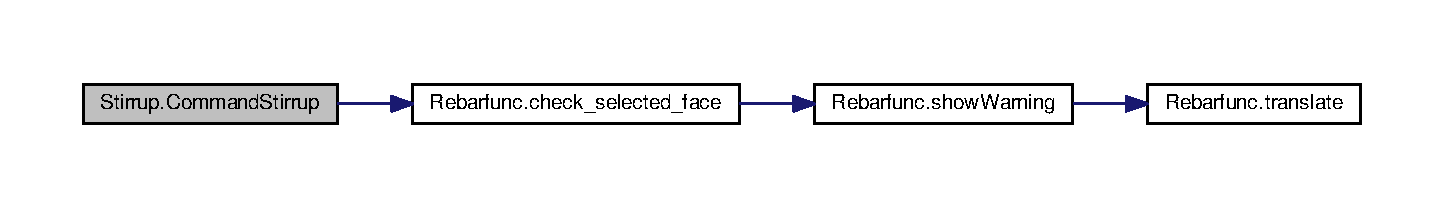
\includegraphics[width=350pt]{namespaceStirrup_a3863ce61c716794557101a50f41597b5_cgraph}
\end{center}
\end{figure}




Here is the caller graph for this function\+:\nopagebreak
\begin{figure}[H]
\begin{center}
\leavevmode
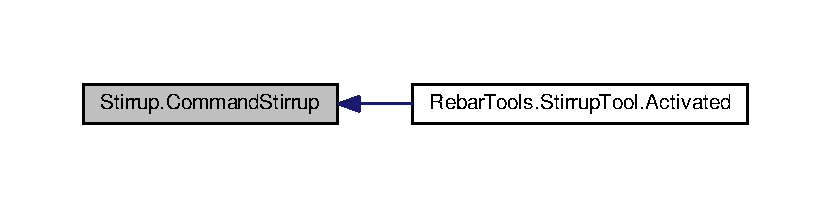
\includegraphics[width=350pt]{namespaceStirrup_a3863ce61c716794557101a50f41597b5_icgraph}
\end{center}
\end{figure}


\index{Stirrup@{Stirrup}!edit\+Dialog@{edit\+Dialog}}
\index{edit\+Dialog@{edit\+Dialog}!Stirrup@{Stirrup}}
\subsubsection[{\texorpdfstring{edit\+Dialog(vobj)}{editDialog(vobj)}}]{\setlength{\rightskip}{0pt plus 5cm}def Stirrup.\+edit\+Dialog (
\begin{DoxyParamCaption}
\item[{}]{vobj}
\end{DoxyParamCaption}
)}\hypertarget{namespaceStirrup_a8ebd17322b7f4f5fe9e50bd578ba670d}{}\label{namespaceStirrup_a8ebd17322b7f4f5fe9e50bd578ba670d}


Definition at line \hyperlink{Stirrup_8py_source_l00327}{327} of file \hyperlink{Stirrup_8py_source}{Stirrup.\+py}.


\begin{DoxyCode}
\hypertarget{namespaceStirrup.tex_l00327}{}\hyperlink{namespaceStirrup_a8ebd17322b7f4f5fe9e50bd578ba670d}{00327} \textcolor{keyword}{def }\hyperlink{namespaceStirrup_a8ebd17322b7f4f5fe9e50bd578ba670d}{editDialog}(vobj):
00328     FreeCADGui.Control.closeDialog()
00329     obj = \hyperlink{classStirrup_1_1__StirrupTaskPanel}{\_StirrupTaskPanel}(vobj.Object)
00330     obj.form.frontCover.setText(str(vobj.Object.FrontCover))
00331     obj.form.l\_sideCover.setText(str(vobj.Object.LeftCover))
00332     obj.form.r\_sideCover.setText(str(vobj.Object.RightCover))
00333     obj.form.t\_sideCover.setText(str(vobj.Object.TopCover))
00334     obj.form.b\_sideCover.setText(str(vobj.Object.BottomCover))
00335     obj.form.diameter.setText(str(vobj.Object.Diameter))
00336     obj.form.bentAngle.setCurrentIndex(obj.form.bentAngle.findText(str(vobj.Object.BentAngle)))
00337     obj.form.bentFactor.setValue(vobj.Object.BentFactor)
00338     obj.form.rounding.setValue(vobj.Object.Rounding)
00339     \textcolor{keywordflow}{if} vobj.Object.AmountCheck:
00340         obj.form.amount.setValue(vobj.Object.Amount)
00341     \textcolor{keywordflow}{else}:
00342         obj.form.amount\_radio.setChecked(\textcolor{keyword}{False})
00343         obj.form.spacing\_radio.setChecked(\textcolor{keyword}{True})
00344         obj.form.amount.setDisabled(\textcolor{keyword}{True})
00345         obj.form.spacing.setEnabled(\textcolor{keyword}{True})
00346         obj.form.spacing.setText(str(vobj.Object.TrueSpacing))
00347     \textcolor{comment}{#obj.form.PickSelectedFace.setVisible(False)}
00348     FreeCADGui.Control.showDialog(obj)
00349 
\end{DoxyCode}
\index{Stirrup@{Stirrup}!edit\+Stirrup@{edit\+Stirrup}}
\index{edit\+Stirrup@{edit\+Stirrup}!Stirrup@{Stirrup}}
\subsubsection[{\texorpdfstring{edit\+Stirrup(\+Rebar, l\+\_\+cover, r\+\_\+cover, t\+\_\+cover, b\+\_\+cover, f\+\_\+cover, bent\+Angle, bent\+Factor, diameter, rounding, amount\+\_\+spacing\+\_\+check, amount\+\_\+spacing\+\_\+value, structure=\+None, facename=\+None)}{editStirrup(Rebar, l_cover, r_cover, t_cover, b_cover, f_cover, bentAngle, bentFactor, diameter, rounding, amount_spacing_check, amount_spacing_value, structure=None, facename=None)}}]{\setlength{\rightskip}{0pt plus 5cm}def Stirrup.\+edit\+Stirrup (
\begin{DoxyParamCaption}
\item[{}]{Rebar, }
\item[{}]{l\+\_\+cover, }
\item[{}]{r\+\_\+cover, }
\item[{}]{t\+\_\+cover, }
\item[{}]{b\+\_\+cover, }
\item[{}]{f\+\_\+cover, }
\item[{}]{bent\+Angle, }
\item[{}]{bent\+Factor, }
\item[{}]{diameter, }
\item[{}]{rounding, }
\item[{}]{amount\+\_\+spacing\+\_\+check, }
\item[{}]{amount\+\_\+spacing\+\_\+value, }
\item[{}]{structure = {\ttfamily None}, }
\item[{}]{facename = {\ttfamily None}}
\end{DoxyParamCaption}
)}\hypertarget{namespaceStirrup_a1f6d278ace7fe116895dba342e2a3573}{}\label{namespaceStirrup_a1f6d278ace7fe116895dba342e2a3573}


Definition at line \hyperlink{Stirrup_8py_source_l00281}{281} of file \hyperlink{Stirrup_8py_source}{Stirrup.\+py}.


\begin{DoxyCode}
\hypertarget{namespaceStirrup.tex_l00281}{}\hyperlink{namespaceStirrup_a1f6d278ace7fe116895dba342e2a3573}{00281}         amount\_spacing\_check, amount\_spacing\_value, structure = \textcolor{keywordtype}{None}, facename = \textcolor{keywordtype}{None}):
00282     sketch = Rebar.Base
00283     \textcolor{keywordflow}{if} structure \textcolor{keywordflow}{and} facename:
00284         sketch.Support = [(structure, facename)]
00285     \textcolor{comment}{# Check if sketch support is empty.}
00286     \textcolor{keywordflow}{if} \textcolor{keywordflow}{not} sketch.Support:
00287         \hyperlink{namespaceRebarfunc_a2278a0602d46a62953af1fcf2e574a94}{showWarning}(\textcolor{stringliteral}{"You have checked remove external geometry of base sketchs when needed.\(\backslash\)nTo
       unchecked Edit->Preferences->Arch."})
00288         \textcolor{keywordflow}{return}
00289     \textcolor{comment}{# Assigned values}
00290     facename = sketch.Support[0][1][0]
00291     structure = sketch.Support[0][0]
00292     face = structure.Shape.Faces[\hyperlink{namespaceRebarfunc_a3885b3b63e3a41508ac79bc7550cf301}{getFaceNumber}(facename) - 1]
00293     \textcolor{comment}{#StructurePRM = getTrueParametersOfStructure(structure)}
00294     \textcolor{comment}{# Get parameters of the face where sketch of rebar is drawn}
00295     FacePRM = \hyperlink{namespaceRebarfunc_a92122b3d7cedd3d47bb63380a5ac4d08}{getParametersOfFace}(structure, facename, \textcolor{keyword}{False})
00296     FaceNormal = face.normalAt(0, 0)
00297     \textcolor{comment}{#FaceNormal = face.Placement.Rotation.inverted().multVec(FaceNormal)}
00298     \textcolor{comment}{# Calculate the coordinates value of Stirrup rebar}
00299     points = \hyperlink{namespaceStirrup_aa6df5118806bfe9d3a799e1bf549bb0a}{getpointsOfStirrup}(FacePRM, l\_cover, r\_cover, t\_cover, b\_cover, bentAngle, 
      bentFactor, diameter, rounding, FaceNormal)
00300     Rebar.Base.Points = points
00301     FreeCAD.ActiveDocument.recompute()
00302     Rebar.Direction = FaceNormal.negative()
00303     Rebar.OffsetStart = f\_cover
00304     Rebar.OffsetEnd = f\_cover
00305     Rebar.BentAngle = bentAngle
00306     Rebar.BentFactor = bentFactor
00307     Rebar.Rounding = rounding
00308     Rebar.Diameter = diameter
00309     \textcolor{keywordflow}{if} amount\_spacing\_check:
00310         Rebar.Amount = amount\_spacing\_value
00311         FreeCAD.ActiveDocument.recompute()
00312         Rebar.AmountCheck = \textcolor{keyword}{True}
00313     \textcolor{keywordflow}{else}:
00314         size = (ArchCommands.projectToVector(structure.Shape.copy(), face.normalAt(0, 0))).Length
00315         Rebar.Amount = int((size - diameter) / amount\_spacing\_value)
00316         FreeCAD.ActiveDocument.recompute()
00317         Rebar.AmountCheck = \textcolor{keyword}{False}
00318     Rebar.FrontCover = f\_cover
00319     Rebar.LeftCover = l\_cover
00320     Rebar.RightCover = r\_cover
00321     Rebar.TopCover = t\_cover
00322     Rebar.BottomCover = b\_cover
00323     Rebar.TrueSpacing = amount\_spacing\_value
00324     FreeCAD.ActiveDocument.recompute()
00325     \textcolor{keywordflow}{return} Rebar
00326 
\end{DoxyCode}


Here is the call graph for this function\+:\nopagebreak
\begin{figure}[H]
\begin{center}
\leavevmode
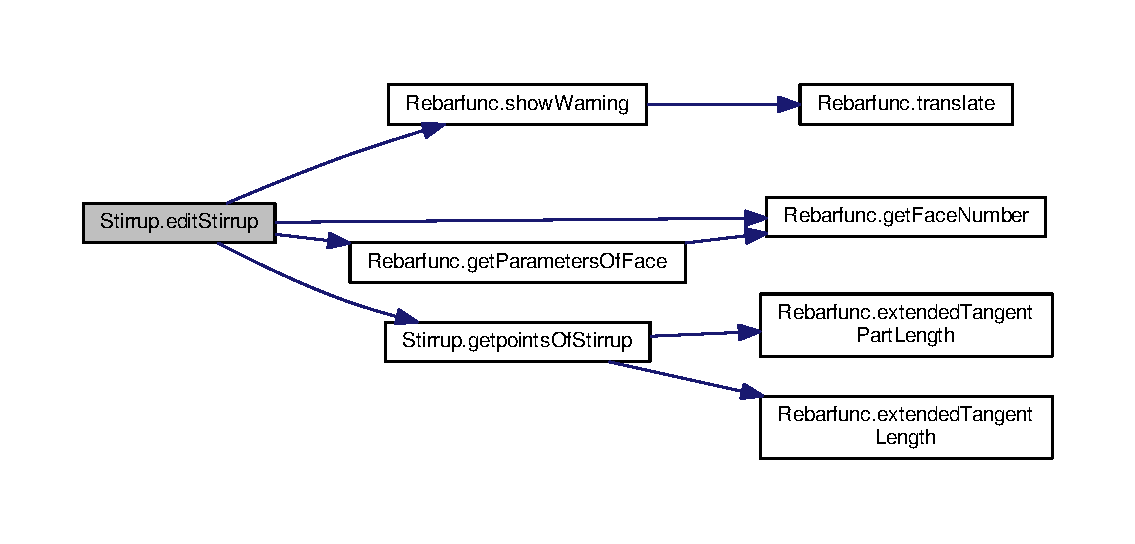
\includegraphics[width=350pt]{namespaceStirrup_a1f6d278ace7fe116895dba342e2a3573_cgraph}
\end{center}
\end{figure}




Here is the caller graph for this function\+:\nopagebreak
\begin{figure}[H]
\begin{center}
\leavevmode
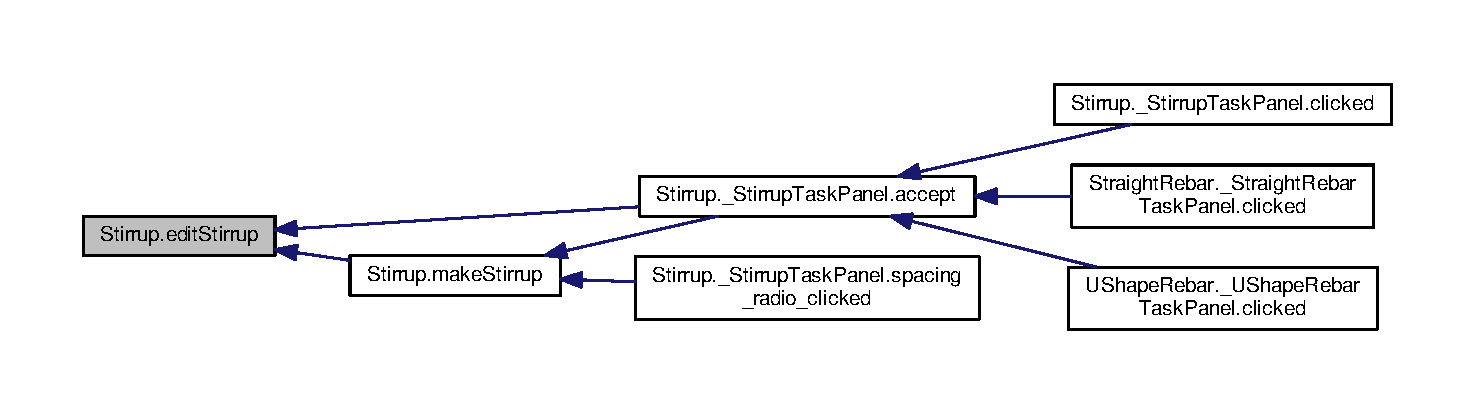
\includegraphics[width=350pt]{namespaceStirrup_a1f6d278ace7fe116895dba342e2a3573_icgraph}
\end{center}
\end{figure}


\index{Stirrup@{Stirrup}!getpoints\+Of\+Stirrup@{getpoints\+Of\+Stirrup}}
\index{getpoints\+Of\+Stirrup@{getpoints\+Of\+Stirrup}!Stirrup@{Stirrup}}
\subsubsection[{\texorpdfstring{getpoints\+Of\+Stirrup(\+Face\+P\+R\+M, l\+\_\+cover, r\+\_\+cover, t\+\_\+cover, b\+\_\+cover, bent\+Angle, bent\+Factor, diameter, rounding, facenormal)}{getpointsOfStirrup(FacePRM, l_cover, r_cover, t_cover, b_cover, bentAngle, bentFactor, diameter, rounding, facenormal)}}]{\setlength{\rightskip}{0pt plus 5cm}def Stirrup.\+getpoints\+Of\+Stirrup (
\begin{DoxyParamCaption}
\item[{}]{Face\+P\+RM, }
\item[{}]{l\+\_\+cover, }
\item[{}]{r\+\_\+cover, }
\item[{}]{t\+\_\+cover, }
\item[{}]{b\+\_\+cover, }
\item[{}]{bent\+Angle, }
\item[{}]{bent\+Factor, }
\item[{}]{diameter, }
\item[{}]{rounding, }
\item[{}]{facenormal}
\end{DoxyParamCaption}
)}\hypertarget{namespaceStirrup_aa6df5118806bfe9d3a799e1bf549bb0a}{}\label{namespaceStirrup_aa6df5118806bfe9d3a799e1bf549bb0a}
\begin{DoxyVerb}getpointsOfStirrup(FacePRM, LeftCover, RightCover, TopCover, BottomCover, BentAngle, BentFactor, Diameter, Rounding, FaceNormal):
Return the coordinates points of the Stirrup in the form of array.\end{DoxyVerb}
 

Definition at line \hyperlink{Stirrup_8py_source_l00040}{40} of file \hyperlink{Stirrup_8py_source}{Stirrup.\+py}.


\begin{DoxyCode}
\hypertarget{namespaceStirrup.tex_l00040}{}\hyperlink{namespaceStirrup_aa6df5118806bfe9d3a799e1bf549bb0a}{00040} \textcolor{keyword}{def }\hyperlink{namespaceStirrup_aa6df5118806bfe9d3a799e1bf549bb0a}{getpointsOfStirrup}(FacePRM, l\_cover, r\_cover, t\_cover, b\_cover, bentAngle, 
      bentFactor, diameter, rounding, facenormal):
00041     \textcolor{stringliteral}{""" getpointsOfStirrup(FacePRM, LeftCover, RightCover, TopCover, BottomCover, BentAngle, BentFactor,
       Diameter, Rounding, FaceNormal):}
00042 \textcolor{stringliteral}{    Return the coordinates points of the Stirrup in the form of array."""}
00043     angle = 180 - bentAngle
00044     tangent\_part\_length = \hyperlink{namespaceRebarfunc_aaeecb468e0fcfc5eee69d6a24c5c5aef}{extendedTangentPartLength}(rounding, diameter, angle)
00045     tangent\_length = \hyperlink{namespaceRebarfunc_ab5637ab0a8e202409ee8657d39ca87a0}{extendedTangentLength}(rounding, diameter, angle)
00046     \textcolor{keywordflow}{if} round(facenormal[0]) \textcolor{keywordflow}{in} \{1,-1\}:
00047         x1 = FacePRM[1][0]
00048         y1 = FacePRM[1][1] - FacePRM[0][0] / 2 + l\_cover
00049         z1 = FacePRM[1][2] + FacePRM[0][1] / 2 - t\_cover + tangent\_part\_length
00050         y2 = FacePRM[1][1] - FacePRM[0][0] / 2 + l\_cover
00051         z2 = FacePRM[1][2] - FacePRM[0][1] / 2 + b\_cover
00052         y3 = FacePRM[1][1] + FacePRM[0][0] / 2 - r\_cover
00053         z3 = FacePRM[1][2] - FacePRM[0][1] / 2 + b\_cover
00054         y4 = FacePRM[1][1] + FacePRM[0][0] / 2 - r\_cover
00055         z4 = FacePRM[1][2] + FacePRM[0][1] / 2 - t\_cover
00056         y5 = FacePRM[1][1] - FacePRM[0][0] / 2 + l\_cover - tangent\_part\_length
00057         z5 = FacePRM[1][2] + FacePRM[0][1] / 2 - t\_cover
00058         side\_length = abs(y5 - y4) - tangent\_part\_length
00059         normal\_dis = (diameter * (side\_length + tangent\_part\_length)) / side\_length
00060         x2 = x1 - normal\_dis / 4
00061         x3 = x2 - normal\_dis / 4
00062         x4 = x3 - normal\_dis / 4
00063         x5 = x4 - normal\_dis / 4
00064         x0 = x1 + normal\_dis / 4
00065         y0 = y1 + (tangent\_length + bentFactor * diameter) * math.sin(math.radians(angle))
00066         z0 = z1 - (tangent\_length + bentFactor * diameter) * math.cos(math.radians(angle))
00067         x6 = x5 - normal\_dis / 4
00068         y6 = y5 + (tangent\_length + bentFactor * diameter) * math.sin(math.radians(90 - angle))
00069         z6 = z5 - (tangent\_length + bentFactor * diameter) * math.cos(math.radians(90 - angle))
00070     \textcolor{keywordflow}{elif} round(facenormal[1]) \textcolor{keywordflow}{in} \{1,-1\}:
00071         x1 = FacePRM[1][0] - FacePRM[0][0] / 2 + l\_cover
00072         y1 = FacePRM[1][1]
00073         z1 = FacePRM[1][2] + FacePRM[0][1] / 2 - t\_cover + tangent\_part\_length
00074         x2 = FacePRM[1][0] - FacePRM[0][0] / 2 + l\_cover
00075         z2 = FacePRM[1][2] - FacePRM[0][1] / 2 + b\_cover
00076         x3 = FacePRM[1][0] + FacePRM[0][0] / 2 - r\_cover
00077         z3 = FacePRM[1][2] - FacePRM[0][1] / 2 + b\_cover
00078         x4 = FacePRM[1][0] + FacePRM[0][0] / 2 - r\_cover
00079         z4 = FacePRM[1][2] + FacePRM[0][1] / 2 - t\_cover
00080         x5 = FacePRM[1][0] - FacePRM[0][0] / 2 + l\_cover - tangent\_part\_length
00081         z5 = FacePRM[1][2] + FacePRM[0][1] / 2 - t\_cover
00082         side\_length = abs(x5 - x4) - tangent\_part\_length
00083         normal\_dis = (diameter * (side\_length + tangent\_part\_length)) / side\_length
00084         y2 = y1 - normal\_dis / 4
00085         y3 = y2 - normal\_dis / 4
00086         y4 = y3 - normal\_dis / 4
00087         y5 = y4 - normal\_dis / 4
00088         y0 = y1 + normal\_dis / 4
00089         x0 = x1 + (tangent\_length + bentFactor * diameter) * math.sin(math.radians(angle))
00090         z0 = z1 - (tangent\_length + bentFactor * diameter) * math.cos(math.radians(angle))
00091         x6 = x5 + (tangent\_length + bentFactor * diameter) * math.sin(math.radians(90 - angle))
00092         y6 = y5 - normal\_dis / 4
00093         z6 = z5 - (tangent\_length + bentFactor * diameter) * math.cos(math.radians(90 - angle))
00094     \textcolor{keywordflow}{elif} round(facenormal[2]) \textcolor{keywordflow}{in} \{1,-1\}:
00095         x1 = FacePRM[1][0] - FacePRM[0][0] / 2 + l\_cover
00096         y1 = FacePRM[1][1] + FacePRM[0][1] / 2 - t\_cover + tangent\_part\_length
00097         z1 = FacePRM[1][2]
00098         x2 = FacePRM[1][0] - FacePRM[0][0] / 2 + l\_cover
00099         y2 = FacePRM[1][1] - FacePRM[0][1] / 2 + b\_cover
00100         x3 = FacePRM[1][0] + FacePRM[0][0] / 2 - r\_cover
00101         y3 = FacePRM[1][1] - FacePRM[0][1] / 2 + b\_cover
00102         x4 = FacePRM[1][0] + FacePRM[0][0] / 2 - r\_cover
00103         y4 = FacePRM[1][1] + FacePRM[0][1] / 2 - t\_cover
00104         x5 = FacePRM[1][0] - FacePRM[0][0] / 2 + l\_cover - tangent\_part\_length
00105         y5 = FacePRM[1][1] + FacePRM[0][1] / 2 - t\_cover
00106         side\_length = abs(x5 - x4) - tangent\_part\_length
00107         normal\_dis = (diameter * (side\_length + tangent\_part\_length)) / side\_length
00108         z2 = z1 - normal\_dis / 4
00109         z3 = z2 - normal\_dis / 4
00110         z4 = z3 - normal\_dis / 4
00111         z5 = z4 - normal\_dis / 4
00112         z0 = z1 + normal\_dis / 4
00113         x0 = x1 + (tangent\_length + bentFactor * diameter) * math.sin(math.radians(angle))
00114         y0 = y1 - (tangent\_length + bentFactor * diameter) * math.cos(math.radians(angle))
00115         x6 = x5 + (tangent\_length + bentFactor * diameter) * math.sin(math.radians(90 - angle))
00116         y6 = y5 - (tangent\_length + bentFactor * diameter) * math.cos(math.radians(90 - angle))
00117         z6 = z5 - normal\_dis / 4
00118     \textcolor{keywordflow}{return} [FreeCAD.Vector(x0, y0, z0), FreeCAD.Vector(x1, y1, z1),\(\backslash\)
00119             FreeCAD.Vector(x2, y2, z2), FreeCAD.Vector(x3, y3, z3),\(\backslash\)
00120             FreeCAD.Vector(x4, y4, z4), FreeCAD.Vector(x5, y5, z5),\(\backslash\)
00121             FreeCAD.Vector(x6, y6, z6)]
00122 
\end{DoxyCode}


Here is the call graph for this function\+:\nopagebreak
\begin{figure}[H]
\begin{center}
\leavevmode
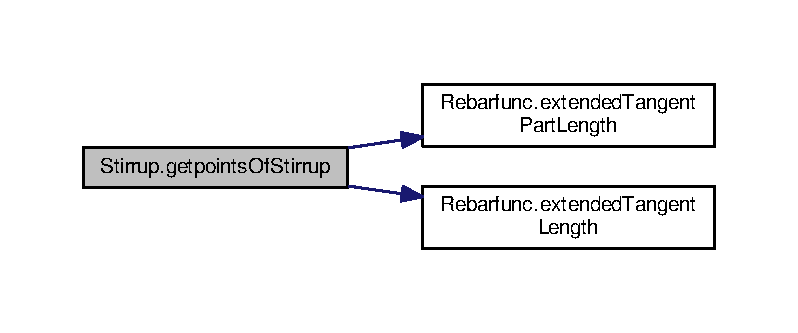
\includegraphics[width=350pt]{namespaceStirrup_aa6df5118806bfe9d3a799e1bf549bb0a_cgraph}
\end{center}
\end{figure}




Here is the caller graph for this function\+:\nopagebreak
\begin{figure}[H]
\begin{center}
\leavevmode
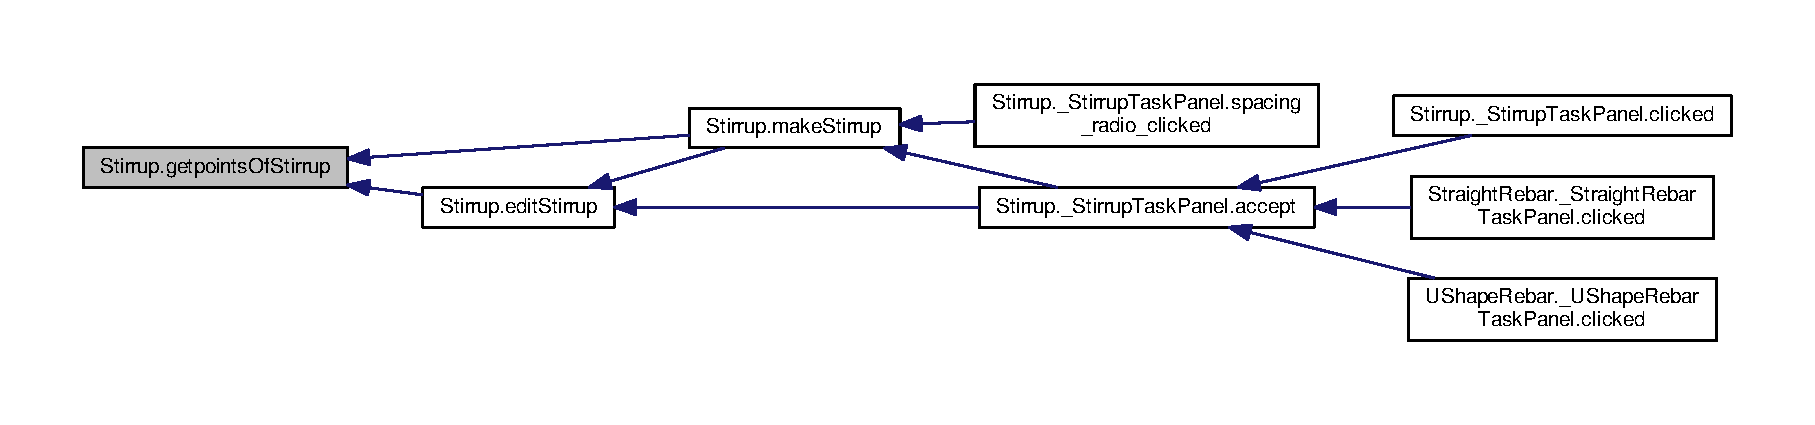
\includegraphics[width=350pt]{namespaceStirrup_aa6df5118806bfe9d3a799e1bf549bb0a_icgraph}
\end{center}
\end{figure}


\index{Stirrup@{Stirrup}!make\+Stirrup@{make\+Stirrup}}
\index{make\+Stirrup@{make\+Stirrup}!Stirrup@{Stirrup}}
\subsubsection[{\texorpdfstring{make\+Stirrup(l\+\_\+cover, r\+\_\+cover, t\+\_\+cover, b\+\_\+cover, f\+\_\+cover, bent\+Angle, bent\+Factor, diameter, rounding, amount\+\_\+spacing\+\_\+check, amount\+\_\+spacing\+\_\+value, structure=\+None, facename=\+None)}{makeStirrup(l_cover, r_cover, t_cover, b_cover, f_cover, bentAngle, bentFactor, diameter, rounding, amount_spacing_check, amount_spacing_value, structure=None, facename=None)}}]{\setlength{\rightskip}{0pt plus 5cm}def Stirrup.\+make\+Stirrup (
\begin{DoxyParamCaption}
\item[{}]{l\+\_\+cover, }
\item[{}]{r\+\_\+cover, }
\item[{}]{t\+\_\+cover, }
\item[{}]{b\+\_\+cover, }
\item[{}]{f\+\_\+cover, }
\item[{}]{bent\+Angle, }
\item[{}]{bent\+Factor, }
\item[{}]{diameter, }
\item[{}]{rounding, }
\item[{}]{amount\+\_\+spacing\+\_\+check, }
\item[{}]{amount\+\_\+spacing\+\_\+value, }
\item[{}]{structure = {\ttfamily None}, }
\item[{}]{facename = {\ttfamily None}}
\end{DoxyParamCaption}
)}\hypertarget{namespaceStirrup_a705fc121e2af9c8ac05eb299f4fb9f2f}{}\label{namespaceStirrup_a705fc121e2af9c8ac05eb299f4fb9f2f}
\begin{DoxyVerb}makeStirrup(LeftCover, RightCover, TopCover, BottomCover, FrontCover, BentAngle,
BentFactor, Diameter, Rounding, AmountSpacingCheck, AmountSpacingValue, Structure, Facename):
Adds the Stirrup reinforcement bar to the selected structural object.\end{DoxyVerb}
 

Definition at line \hyperlink{Stirrup_8py_source_l00210}{210} of file \hyperlink{Stirrup_8py_source}{Stirrup.\+py}.


\begin{DoxyCode}
\hypertarget{namespaceStirrup.tex_l00210}{}\hyperlink{namespaceStirrup_a705fc121e2af9c8ac05eb299f4fb9f2f}{00210}         amount\_spacing\_check, amount\_spacing\_value, structure = \textcolor{keywordtype}{None}, facename = \textcolor{keywordtype}{None}):
00211     \textcolor{stringliteral}{""" makeStirrup(LeftCover, RightCover, TopCover, BottomCover, FrontCover, BentAngle,}
00212 \textcolor{stringliteral}{    BentFactor, Diameter, Rounding, AmountSpacingCheck, AmountSpacingValue, Structure, Facename):}
00213 \textcolor{stringliteral}{    Adds the Stirrup reinforcement bar to the selected structural object."""}
00214     \textcolor{keywordflow}{if} \textcolor{keywordflow}{not} structure \textcolor{keywordflow}{and} \textcolor{keywordflow}{not} facename:
00215         selected\_obj = FreeCADGui.Selection.getSelectionEx()[0]
00216         structure = selected\_obj.Object
00217         facename = selected\_obj.SubElementNames[0]
00218     face = structure.Shape.Faces[\hyperlink{namespaceRebarfunc_a3885b3b63e3a41508ac79bc7550cf301}{getFaceNumber}(facename) - 1]
00219     \textcolor{comment}{#StructurePRM = getTrueParametersOfStructure(structure)}
00220     FacePRM = \hyperlink{namespaceRebarfunc_a92122b3d7cedd3d47bb63380a5ac4d08}{getParametersOfFace}(structure, facename, \textcolor{keyword}{False})
00221     FaceNormal = face.normalAt(0,0)
00222     \textcolor{comment}{#FaceNormal = face.Placement.Rotation.inverted().multVec(FaceNormal)}
00223     \textcolor{keywordflow}{if} \textcolor{keywordflow}{not} FacePRM:
00224         FreeCAD.Console.PrintError(\textcolor{stringliteral}{"Cannot identified shape or from which base object sturctural element is
       derived\(\backslash\)n"})
00225         \textcolor{keywordflow}{return}
00226     \textcolor{comment}{# Calculate the coordinate values of Stirrup}
00227     points = \hyperlink{namespaceStirrup_aa6df5118806bfe9d3a799e1bf549bb0a}{getpointsOfStirrup}(FacePRM, l\_cover, r\_cover, t\_cover, b\_cover, bentAngle, 
      bentFactor, diameter, rounding, FaceNormal)
00228     \textcolor{keyword}{import} Draft
00229     line = Draft.makeWire(points, closed = \textcolor{keyword}{False}, face = \textcolor{keyword}{True}, support = \textcolor{keywordtype}{None})
00230     \textcolor{keyword}{import} Arch
00231     line.Support = [(structure, facename)]
00232     \textcolor{keywordflow}{if} amount\_spacing\_check:
00233         rebar = Arch.makeRebar(structure, line, diameter, amount\_spacing\_value, f\_cover)
00234     \textcolor{keywordflow}{else}:
00235         size = (ArchCommands.projectToVector(structure.Shape.copy(), face.normalAt(0, 0))).Length
00236         rebar = Arch.makeRebar(structure, line, diameter,\(\backslash\)
00237             int((size - diameter) / amount\_spacing\_value), f\_cover)
00238     rebar.Direction = FaceNormal.negative()
00239     rebar.Rounding = rounding
00240     \textcolor{comment}{# Adds properties to the rebar object}
00241     rebar.ViewObject.addProperty(\textcolor{stringliteral}{"App::PropertyString"}, \textcolor{stringliteral}{"RebarShape"}, \textcolor{stringliteral}{"RebarDialog"},\(\backslash\)
00242         QT\_TRANSLATE\_NOOP(\textcolor{stringliteral}{"App::Property"},\textcolor{stringliteral}{"Shape of rebar"})).RebarShape = \textcolor{stringliteral}{"Stirrup"}
00243     rebar.ViewObject.setEditorMode(\textcolor{stringliteral}{"RebarShape"}, 2)
00244     rebar.addProperty(\textcolor{stringliteral}{"App::PropertyDistance"}, \textcolor{stringliteral}{"LeftCover"}, \textcolor{stringliteral}{"RebarDialog"},\(\backslash\)
00245         QT\_TRANSLATE\_NOOP(\textcolor{stringliteral}{"App::Property"}, \textcolor{stringliteral}{"Left Side cover of rebar"})).LeftCover = l\_cover
00246     rebar.setEditorMode(\textcolor{stringliteral}{"LeftCover"}, 2)
00247     rebar.addProperty(\textcolor{stringliteral}{"App::PropertyDistance"}, \textcolor{stringliteral}{"RightCover"}, \textcolor{stringliteral}{"RebarDialog"},\(\backslash\)
00248         QT\_TRANSLATE\_NOOP(\textcolor{stringliteral}{"App::Property"}, \textcolor{stringliteral}{"Right Side cover of rebar"})).RightCover = r\_cover
00249     rebar.setEditorMode(\textcolor{stringliteral}{"RightCover"}, 2)
00250     rebar.addProperty(\textcolor{stringliteral}{"App::PropertyDistance"}, \textcolor{stringliteral}{"TopCover"}, \textcolor{stringliteral}{"RebarDialog"},\(\backslash\)
00251         QT\_TRANSLATE\_NOOP(\textcolor{stringliteral}{"App::Property"}, \textcolor{stringliteral}{"Top Side cover of rebar"})).TopCover = t\_cover
00252     rebar.setEditorMode(\textcolor{stringliteral}{"TopCover"}, 2)
00253     rebar.addProperty(\textcolor{stringliteral}{"App::PropertyDistance"}, \textcolor{stringliteral}{"BottomCover"}, \textcolor{stringliteral}{"RebarDialog"},\(\backslash\)
00254         QT\_TRANSLATE\_NOOP(\textcolor{stringliteral}{"App::Property"}, \textcolor{stringliteral}{"Bottom Side cover of rebar"})).BottomCover = b\_cover
00255     rebar.setEditorMode(\textcolor{stringliteral}{"BottomCover"}, 2)
00256     rebar.addProperty(\textcolor{stringliteral}{"App::PropertyDistance"}, \textcolor{stringliteral}{"FrontCover"}, \textcolor{stringliteral}{"RebarDialog"},\(\backslash\)
00257         QT\_TRANSLATE\_NOOP(\textcolor{stringliteral}{"App::Property"}, \textcolor{stringliteral}{"Top cover of rebar"})).FrontCover = f\_cover
00258     rebar.setEditorMode(\textcolor{stringliteral}{"FrontCover"}, 2)
00259     rebar.addProperty(\textcolor{stringliteral}{"App::PropertyInteger"}, \textcolor{stringliteral}{"BentAngle"}, \textcolor{stringliteral}{"RebarDialog"},\(\backslash\)
00260         QT\_TRANSLATE\_NOOP(\textcolor{stringliteral}{"App::Property"}, \textcolor{stringliteral}{"Bent angle between at the end of rebar"})).BentAngle = bentAngle
00261     rebar.setEditorMode(\textcolor{stringliteral}{"BentAngle"}, 2)
00262     rebar.addProperty(\textcolor{stringliteral}{"App::PropertyInteger"}, \textcolor{stringliteral}{"BentFactor"}, \textcolor{stringliteral}{"RebarDialog"},\(\backslash\)
00263         QT\_TRANSLATE\_NOOP(\textcolor{stringliteral}{"App::Property"}, \textcolor{stringliteral}{"Bent Length is the equal to BentFactor * Diameter"})).BentFactor
       = bentFactor
00264     rebar.setEditorMode(\textcolor{stringliteral}{"BentFactor"}, 2)
00265     rebar.addProperty(\textcolor{stringliteral}{"App::PropertyBool"}, \textcolor{stringliteral}{"AmountCheck"}, \textcolor{stringliteral}{"RebarDialog"},\(\backslash\)
00266         QT\_TRANSLATE\_NOOP(\textcolor{stringliteral}{"App::Property"}, \textcolor{stringliteral}{"Amount radio button is checked"})).AmountCheck
00267     rebar.setEditorMode(\textcolor{stringliteral}{"AmountCheck"}, 2)
00268     rebar.addProperty(\textcolor{stringliteral}{"App::PropertyDistance"}, \textcolor{stringliteral}{"TrueSpacing"}, \textcolor{stringliteral}{"RebarDialog"},\(\backslash\)
00269         QT\_TRANSLATE\_NOOP(\textcolor{stringliteral}{"App::Property"}, \textcolor{stringliteral}{"Spacing between of rebars"})).TrueSpacing = amount\_spacing\_value
00270     rebar.setEditorMode(\textcolor{stringliteral}{"TrueSpacing"}, 2)
00271     \textcolor{keywordflow}{if} amount\_spacing\_check:
00272         rebar.AmountCheck = \textcolor{keyword}{True}
00273     \textcolor{keywordflow}{else}:
00274         rebar.AmountCheck = \textcolor{keyword}{False}
00275         rebar.TrueSpacing = amount\_spacing\_value
00276     rebar.Label = \textcolor{stringliteral}{"Stirrup"}
00277     FreeCAD.ActiveDocument.recompute()
00278     \textcolor{keywordflow}{return} rebar
00279 
\end{DoxyCode}


Here is the call graph for this function\+:\nopagebreak
\begin{figure}[H]
\begin{center}
\leavevmode
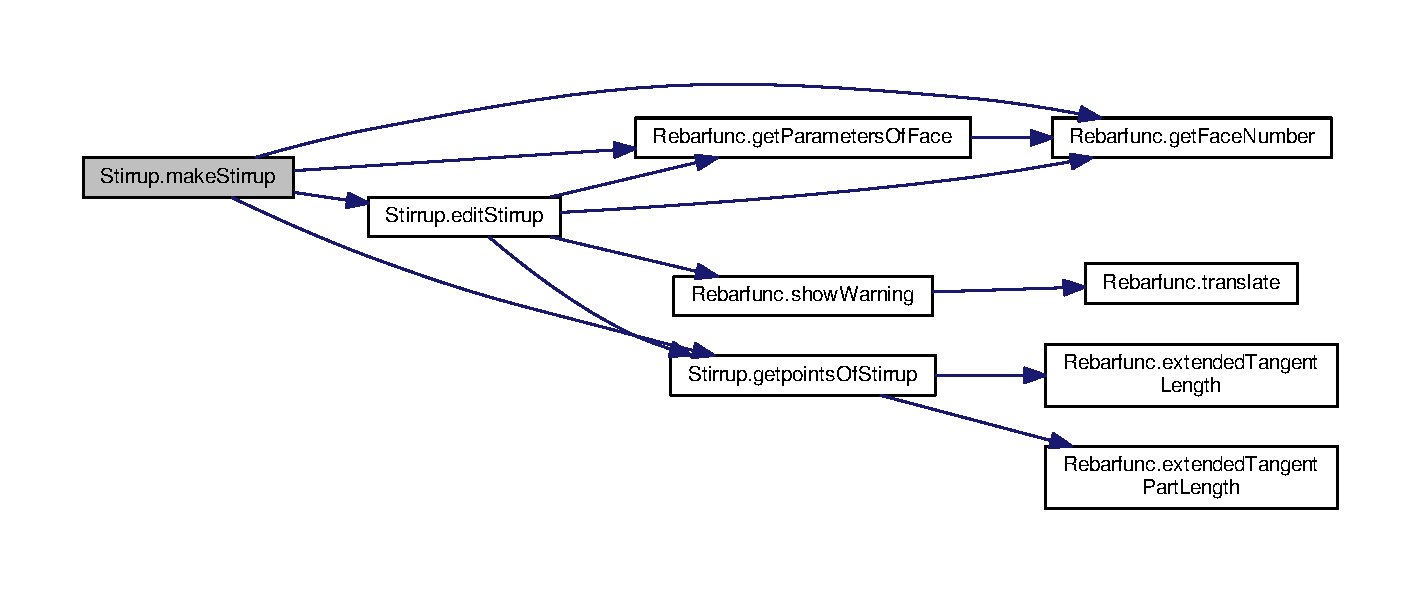
\includegraphics[width=350pt]{namespaceStirrup_a705fc121e2af9c8ac05eb299f4fb9f2f_cgraph}
\end{center}
\end{figure}




Here is the caller graph for this function\+:\nopagebreak
\begin{figure}[H]
\begin{center}
\leavevmode
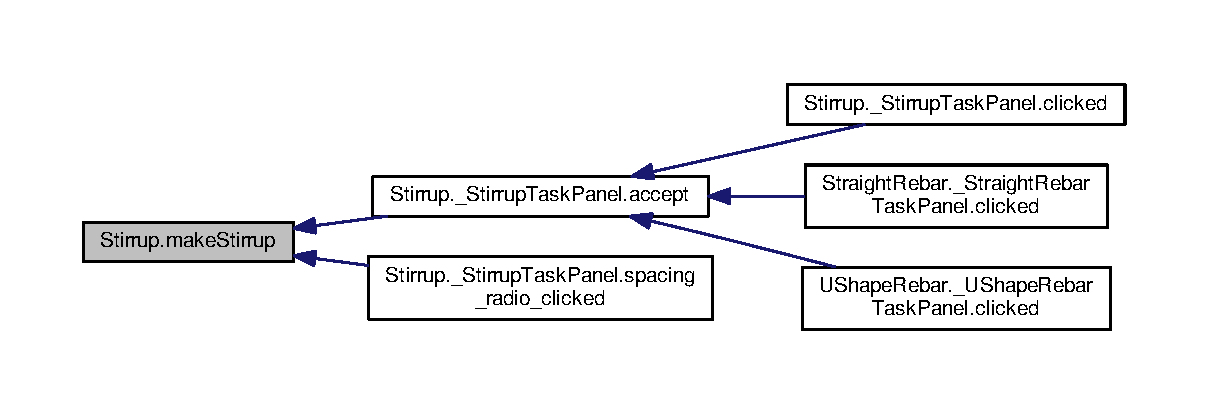
\includegraphics[width=350pt]{namespaceStirrup_a705fc121e2af9c8ac05eb299f4fb9f2f_icgraph}
\end{center}
\end{figure}




\subsection{Variable Documentation}
\index{Stirrup@{Stirrup}!\+\_\+\+\_\+author\+\_\+\+\_\+@{\+\_\+\+\_\+author\+\_\+\+\_\+}}
\index{\+\_\+\+\_\+author\+\_\+\+\_\+@{\+\_\+\+\_\+author\+\_\+\+\_\+}!Stirrup@{Stirrup}}
\subsubsection[{\texorpdfstring{\+\_\+\+\_\+author\+\_\+\+\_\+}{__author__}}]{\setlength{\rightskip}{0pt plus 5cm}string Stirrup.\+\_\+\+\_\+author\+\_\+\+\_\+ = \char`\"{}Amritpal Singh\char`\"{}\hspace{0.3cm}{\ttfamily [private]}}\hypertarget{namespaceStirrup_ad470a52dca49f918ddfef810e749291c}{}\label{namespaceStirrup_ad470a52dca49f918ddfef810e749291c}


Definition at line \hyperlink{Stirrup_8py_source_l00025}{25} of file \hyperlink{Stirrup_8py_source}{Stirrup.\+py}.

\index{Stirrup@{Stirrup}!\+\_\+\+\_\+title\+\_\+\+\_\+@{\+\_\+\+\_\+title\+\_\+\+\_\+}}
\index{\+\_\+\+\_\+title\+\_\+\+\_\+@{\+\_\+\+\_\+title\+\_\+\+\_\+}!Stirrup@{Stirrup}}
\subsubsection[{\texorpdfstring{\+\_\+\+\_\+title\+\_\+\+\_\+}{__title__}}]{\setlength{\rightskip}{0pt plus 5cm}string Stirrup.\+\_\+\+\_\+title\+\_\+\+\_\+ = \char`\"{}Stirrup\+Rebar\char`\"{}\hspace{0.3cm}{\ttfamily [private]}}\hypertarget{namespaceStirrup_aac4f16b6285f67fb07673ac264bac3dc}{}\label{namespaceStirrup_aac4f16b6285f67fb07673ac264bac3dc}


Definition at line \hyperlink{Stirrup_8py_source_l00024}{24} of file \hyperlink{Stirrup_8py_source}{Stirrup.\+py}.

\index{Stirrup@{Stirrup}!\+\_\+\+\_\+url\+\_\+\+\_\+@{\+\_\+\+\_\+url\+\_\+\+\_\+}}
\index{\+\_\+\+\_\+url\+\_\+\+\_\+@{\+\_\+\+\_\+url\+\_\+\+\_\+}!Stirrup@{Stirrup}}
\subsubsection[{\texorpdfstring{\+\_\+\+\_\+url\+\_\+\+\_\+}{__url__}}]{\setlength{\rightskip}{0pt plus 5cm}string Stirrup.\+\_\+\+\_\+url\+\_\+\+\_\+ = \char`\"{}https\+://www.\+freecadweb.\+org\char`\"{}\hspace{0.3cm}{\ttfamily [private]}}\hypertarget{namespaceStirrup_a3b5b07aa3d0183155a2be24e2d0d4a82}{}\label{namespaceStirrup_a3b5b07aa3d0183155a2be24e2d0d4a82}


Definition at line \hyperlink{Stirrup_8py_source_l00026}{26} of file \hyperlink{Stirrup_8py_source}{Stirrup.\+py}.


\hypertarget{namespaceStraightRebar}{}\section{Straight\+Rebar Namespace Reference}
\label{namespaceStraightRebar}\index{Straight\+Rebar@{Straight\+Rebar}}
\subsection*{Classes}
\begin{DoxyCompactItemize}
\item 
class \hyperlink{classStraightRebar_1_1__StraightRebarTaskPanel}{\+\_\+\+Straight\+Rebar\+Task\+Panel}
\end{DoxyCompactItemize}
\subsection*{Functions}
\begin{DoxyCompactItemize}
\item 
def \hyperlink{namespaceStraightRebar_a1873c6f7f59b355a64fdd966ad75f778}{getpoints\+Of\+Straight\+Rebar} (Face\+P\+RM, rt\+\_\+cover, lb\+\_\+cover, cover\+Along, orientation)
\item 
def \hyperlink{namespaceStraightRebar_af6270367d7beae457813e33718d80faf}{make\+Straight\+Rebar} (f\+\_\+cover, cover\+Along, rt\+\_\+cover, lb\+\_\+cover, diameter, amount\+\_\+spacing\+\_\+check, amount\+\_\+spacing\+\_\+value, orientation=\char`\"{}Horizontal\char`\"{}, structure=None, facename=None)
\item 
def \hyperlink{namespaceStraightRebar_ab4c578165b01dd7c7d121e5345de2d7b}{edit\+Straight\+Rebar} (Rebar, f\+\_\+cover, cover\+Along, rt\+\_\+cover, lb\+\_\+cover, diameter, amount\+\_\+spacing\+\_\+check, amount\+\_\+spacing\+\_\+value, orientation, structure=None, facename=None)
\item 
def \hyperlink{namespaceStraightRebar_ad48f93922ce90bb63d051c7c3c794d35}{edit\+Dialog} (vobj)
\item 
def \hyperlink{namespaceStraightRebar_a30f7aada2e2f91cdfae8267da36fe277}{Command\+Straight\+Rebar} ()
\end{DoxyCompactItemize}
\subsection*{Variables}
\begin{DoxyCompactItemize}
\item 
string \hyperlink{namespaceStraightRebar_ab1d45eb17133c23d9d6a3e2a6f2abb8a}{\+\_\+\+\_\+title\+\_\+\+\_\+} = \char`\"{}Straight\+Rebar\char`\"{}
\item 
string \hyperlink{namespaceStraightRebar_ad355d40e3bea5e86c24b6fe813264413}{\+\_\+\+\_\+author\+\_\+\+\_\+} = \char`\"{}Amritpal Singh\char`\"{}
\item 
string \hyperlink{namespaceStraightRebar_aebf23f453d8fabed3a611d14f5e7f057}{\+\_\+\+\_\+url\+\_\+\+\_\+} = \char`\"{}https\+://www.\+freecadweb.\+org\char`\"{}
\end{DoxyCompactItemize}


\subsection{Function Documentation}
\index{Straight\+Rebar@{Straight\+Rebar}!Command\+Straight\+Rebar@{Command\+Straight\+Rebar}}
\index{Command\+Straight\+Rebar@{Command\+Straight\+Rebar}!Straight\+Rebar@{Straight\+Rebar}}
\subsubsection[{\texorpdfstring{Command\+Straight\+Rebar()}{CommandStraightRebar()}}]{\setlength{\rightskip}{0pt plus 5cm}def Straight\+Rebar.\+Command\+Straight\+Rebar (
\begin{DoxyParamCaption}
{}
\end{DoxyParamCaption}
)}\hypertarget{namespaceStraightRebar_a30f7aada2e2f91cdfae8267da36fe277}{}\label{namespaceStraightRebar_a30f7aada2e2f91cdfae8267da36fe277}


Definition at line \hyperlink{StraightRebar_8py_source_l00320}{320} of file \hyperlink{StraightRebar_8py_source}{Straight\+Rebar.\+py}.


\begin{DoxyCode}
\hypertarget{namespaceStraightRebar.tex_l00320}{}\hyperlink{namespaceStraightRebar_a30f7aada2e2f91cdfae8267da36fe277}{00320} \textcolor{keyword}{def }\hyperlink{namespaceStraightRebar_a30f7aada2e2f91cdfae8267da36fe277}{CommandStraightRebar}():
00321     selected\_obj = \hyperlink{namespaceRebarfunc_adae2713855a7e1b4bda04081ae671542}{check\_selected\_face}()
00322     \textcolor{keywordflow}{if} selected\_obj:
00323         FreeCADGui.Control.showDialog(\hyperlink{classStraightRebar_1_1__StraightRebarTaskPanel}{\_StraightRebarTaskPanel}())
00324 \end{DoxyCode}


Here is the call graph for this function\+:\nopagebreak
\begin{figure}[H]
\begin{center}
\leavevmode
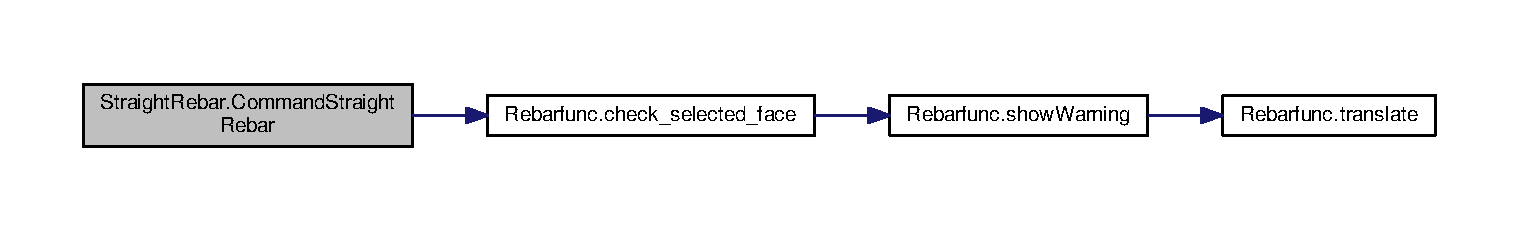
\includegraphics[width=350pt]{namespaceStraightRebar_a30f7aada2e2f91cdfae8267da36fe277_cgraph}
\end{center}
\end{figure}




Here is the caller graph for this function\+:\nopagebreak
\begin{figure}[H]
\begin{center}
\leavevmode
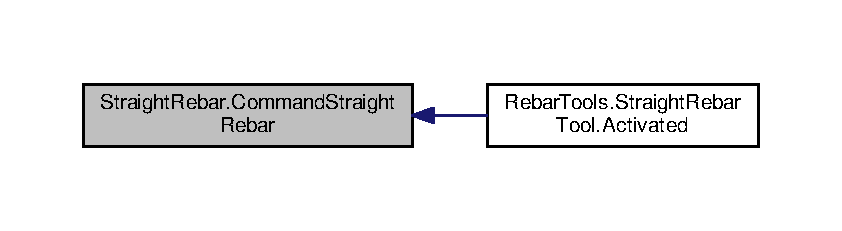
\includegraphics[width=350pt]{namespaceStraightRebar_a30f7aada2e2f91cdfae8267da36fe277_icgraph}
\end{center}
\end{figure}


\index{Straight\+Rebar@{Straight\+Rebar}!edit\+Dialog@{edit\+Dialog}}
\index{edit\+Dialog@{edit\+Dialog}!Straight\+Rebar@{Straight\+Rebar}}
\subsubsection[{\texorpdfstring{edit\+Dialog(vobj)}{editDialog(vobj)}}]{\setlength{\rightskip}{0pt plus 5cm}def Straight\+Rebar.\+edit\+Dialog (
\begin{DoxyParamCaption}
\item[{}]{vobj}
\end{DoxyParamCaption}
)}\hypertarget{namespaceStraightRebar_ad48f93922ce90bb63d051c7c3c794d35}{}\label{namespaceStraightRebar_ad48f93922ce90bb63d051c7c3c794d35}


Definition at line \hyperlink{StraightRebar_8py_source_l00299}{299} of file \hyperlink{StraightRebar_8py_source}{Straight\+Rebar.\+py}.


\begin{DoxyCode}
\hypertarget{namespaceStraightRebar.tex_l00299}{}\hyperlink{namespaceStraightRebar_ad48f93922ce90bb63d051c7c3c794d35}{00299} \textcolor{keyword}{def }\hyperlink{namespaceStraightRebar_ad48f93922ce90bb63d051c7c3c794d35}{editDialog}(vobj):
00300     FreeCADGui.Control.closeDialog()
00301     obj = \hyperlink{classStraightRebar_1_1__StraightRebarTaskPanel}{\_StraightRebarTaskPanel}(vobj.Object)
00302     obj.form.frontCover.setText(str(vobj.Object.FrontCover))
00303     obj.form.r\_sideCover.setText(str(vobj.Object.RightTopCover))
00304     obj.form.l\_sideCover.setText(str(vobj.Object.LeftBottomCover))
00305     obj.form.bottomCover.setText(str(vobj.Object.Cover))
00306     obj.form.diameter.setText(str(vobj.Object.Diameter))
00307     obj.form.orientation.setCurrentIndex(obj.form.orientation.findText(str(vobj.Object.Orientation)))
00308     obj.form.coverAlong.setCurrentIndex(obj.form.coverAlong.findText(str(vobj.Object.CoverAlong)))
00309     \textcolor{keywordflow}{if} vobj.Object.AmountCheck:
00310         obj.form.amount.setValue(vobj.Object.Amount)
00311     \textcolor{keywordflow}{else}:
00312         obj.form.amount\_radio.setChecked(\textcolor{keyword}{False})
00313         obj.form.spacing\_radio.setChecked(\textcolor{keyword}{True})
00314         obj.form.amount.setDisabled(\textcolor{keyword}{True})
00315         obj.form.spacing.setEnabled(\textcolor{keyword}{True})
00316         obj.form.spacing.setText(str(vobj.Object.TrueSpacing))
00317     \textcolor{comment}{#obj.form.PickSelectedFace.setVisible(False)}
00318     FreeCADGui.Control.showDialog(obj)
00319 
\end{DoxyCode}
\index{Straight\+Rebar@{Straight\+Rebar}!edit\+Straight\+Rebar@{edit\+Straight\+Rebar}}
\index{edit\+Straight\+Rebar@{edit\+Straight\+Rebar}!Straight\+Rebar@{Straight\+Rebar}}
\subsubsection[{\texorpdfstring{edit\+Straight\+Rebar(\+Rebar, f\+\_\+cover, cover\+Along, rt\+\_\+cover, lb\+\_\+cover, diameter, amount\+\_\+spacing\+\_\+check, amount\+\_\+spacing\+\_\+value, orientation, structure=\+None, facename=\+None)}{editStraightRebar(Rebar, f_cover, coverAlong, rt_cover, lb_cover, diameter, amount_spacing_check, amount_spacing_value, orientation, structure=None, facename=None)}}]{\setlength{\rightskip}{0pt plus 5cm}def Straight\+Rebar.\+edit\+Straight\+Rebar (
\begin{DoxyParamCaption}
\item[{}]{Rebar, }
\item[{}]{f\+\_\+cover, }
\item[{}]{cover\+Along, }
\item[{}]{rt\+\_\+cover, }
\item[{}]{lb\+\_\+cover, }
\item[{}]{diameter, }
\item[{}]{amount\+\_\+spacing\+\_\+check, }
\item[{}]{amount\+\_\+spacing\+\_\+value, }
\item[{}]{orientation, }
\item[{}]{structure = {\ttfamily None}, }
\item[{}]{facename = {\ttfamily None}}
\end{DoxyParamCaption}
)}\hypertarget{namespaceStraightRebar_ab4c578165b01dd7c7d121e5345de2d7b}{}\label{namespaceStraightRebar_ab4c578165b01dd7c7d121e5345de2d7b}


Definition at line \hyperlink{StraightRebar_8py_source_l00255}{255} of file \hyperlink{StraightRebar_8py_source}{Straight\+Rebar.\+py}.


\begin{DoxyCode}
\hypertarget{namespaceStraightRebar.tex_l00255}{}\hyperlink{namespaceStraightRebar_ab4c578165b01dd7c7d121e5345de2d7b}{00255} \textcolor{keyword}{def }\hyperlink{namespaceStraightRebar_ab4c578165b01dd7c7d121e5345de2d7b}{editStraightRebar}(Rebar, f\_cover, coverAlong, rt\_cover, lb\_cover, diameter, 
      amount\_spacing\_check, amount\_spacing\_value, orientation, structure = None, facename = None):
00256     sketch = Rebar.Base
00257     \textcolor{keywordflow}{if} structure \textcolor{keywordflow}{and} facename:
00258         sketch.Support = [(structure, facename)]
00259         FreeCAD.ActiveDocument.recompute()
00260     \textcolor{comment}{# Check if sketch support is empty.}
00261     \textcolor{keywordflow}{if} \textcolor{keywordflow}{not} sketch.Support:
00262         \hyperlink{namespaceRebarfunc_a2278a0602d46a62953af1fcf2e574a94}{showWarning}(\textcolor{stringliteral}{"You have checked remove external geometry of base sketchs when needed.\(\backslash\)nTo
       unchecked Edit->Preferences->Arch."})
00263         \textcolor{keywordflow}{return}
00264     \textcolor{comment}{# Assigned values}
00265     facename = sketch.Support[0][1][0]
00266     structure = sketch.Support[0][0]
00267     face = structure.Shape.Faces[\hyperlink{namespaceRebarfunc_a3885b3b63e3a41508ac79bc7550cf301}{getFaceNumber}(facename) - 1]
00268     \textcolor{comment}{#StructurePRM = getTrueParametersOfStructure(structure)}
00269     \textcolor{comment}{# Get parameters of the face where sketch of rebar is drawn}
00270     FacePRM = \hyperlink{namespaceRebarfunc_a92122b3d7cedd3d47bb63380a5ac4d08}{getParametersOfFace}(structure, facename)
00271     \textcolor{comment}{# Get points of Striaght rebar}
00272     points = \hyperlink{namespaceStraightRebar_a1873c6f7f59b355a64fdd966ad75f778}{getpointsOfStraightRebar}(FacePRM, rt\_cover, lb\_cover, coverAlong, 
      orientation)
00273     sketch.movePoint(0, 1, points[0], 0)
00274     FreeCAD.ActiveDocument.recompute()
00275     sketch.movePoint(0, 2, points[1], 0)
00276     FreeCAD.ActiveDocument.recompute()
00277     Rebar.OffsetStart = f\_cover
00278     Rebar.OffsetEnd = f\_cover
00279     \textcolor{keywordflow}{if} amount\_spacing\_check:
00280         Rebar.Amount = amount\_spacing\_value
00281         FreeCAD.ActiveDocument.recompute()
00282         Rebar.AmountCheck = \textcolor{keyword}{True}
00283     \textcolor{keywordflow}{else}:
00284         size = (ArchCommands.projectToVector(structure.Shape.copy(), face.normalAt(0, 0))).Length
00285         Rebar.Amount = int((size - diameter) / amount\_spacing\_value)
00286         FreeCAD.ActiveDocument.recompute()
00287         Rebar.AmountCheck = \textcolor{keyword}{False}
00288     Rebar.FrontCover = f\_cover
00289     Rebar.RightTopCover = rt\_cover
00290     Rebar.LeftBottomCover = lb\_cover
00291     Rebar.CoverAlong = coverAlong[0]
00292     Rebar.Cover = coverAlong[1]
00293     Rebar.TrueSpacing = amount\_spacing\_value
00294     Rebar.Diameter = diameter
00295     Rebar.Orientation = orientation
00296     FreeCAD.ActiveDocument.recompute()
00297     \textcolor{keywordflow}{return} Rebar
00298 
\end{DoxyCode}


Here is the call graph for this function\+:\nopagebreak
\begin{figure}[H]
\begin{center}
\leavevmode
\includegraphics[width=350pt]{namespaceStraightRebar_ab4c578165b01dd7c7d121e5345de2d7b_cgraph}
\end{center}
\end{figure}




Here is the caller graph for this function\+:\nopagebreak
\begin{figure}[H]
\begin{center}
\leavevmode
\includegraphics[width=350pt]{namespaceStraightRebar_ab4c578165b01dd7c7d121e5345de2d7b_icgraph}
\end{center}
\end{figure}


\index{Straight\+Rebar@{Straight\+Rebar}!getpoints\+Of\+Straight\+Rebar@{getpoints\+Of\+Straight\+Rebar}}
\index{getpoints\+Of\+Straight\+Rebar@{getpoints\+Of\+Straight\+Rebar}!Straight\+Rebar@{Straight\+Rebar}}
\subsubsection[{\texorpdfstring{getpoints\+Of\+Straight\+Rebar(\+Face\+P\+R\+M, rt\+\_\+cover, lb\+\_\+cover, cover\+Along, orientation)}{getpointsOfStraightRebar(FacePRM, rt_cover, lb_cover, coverAlong, orientation)}}]{\setlength{\rightskip}{0pt plus 5cm}def Straight\+Rebar.\+getpoints\+Of\+Straight\+Rebar (
\begin{DoxyParamCaption}
\item[{}]{Face\+P\+RM, }
\item[{}]{rt\+\_\+cover, }
\item[{}]{lb\+\_\+cover, }
\item[{}]{cover\+Along, }
\item[{}]{orientation}
\end{DoxyParamCaption}
)}\hypertarget{namespaceStraightRebar_a1873c6f7f59b355a64fdd966ad75f778}{}\label{namespaceStraightRebar_a1873c6f7f59b355a64fdd966ad75f778}
\begin{DoxyVerb}getpointsOfStraightRebar(FacePRM, RightTopcover, LeftBottomcover, CoverAlong, Orientation):
Return points of the Straight rebar in the form of array for sketch.

Case I: When Orientation is 'Horizontal':
    We have two option in CoverAlong i.e. 'Bottom Side' or 'Top Side'
Case II: When Orientation is 'Vertical':
    We have two option in CoverAlong i.e. 'Left Side' or 'Right Side'
\end{DoxyVerb}
 

Definition at line \hyperlink{StraightRebar_8py_source_l00040}{40} of file \hyperlink{StraightRebar_8py_source}{Straight\+Rebar.\+py}.


\begin{DoxyCode}
\hypertarget{namespaceStraightRebar.tex_l00040}{}\hyperlink{namespaceStraightRebar_a1873c6f7f59b355a64fdd966ad75f778}{00040} \textcolor{keyword}{def }\hyperlink{namespaceStraightRebar_a1873c6f7f59b355a64fdd966ad75f778}{getpointsOfStraightRebar}(FacePRM, rt\_cover, lb\_cover, coverAlong, orientation):
00041     \textcolor{stringliteral}{""" getpointsOfStraightRebar(FacePRM, RightTopcover, LeftBottomcover, CoverAlong, Orientation):}
00042 \textcolor{stringliteral}{    Return points of the Straight rebar in the form of array for sketch.}
00043 \textcolor{stringliteral}{}
00044 \textcolor{stringliteral}{    Case I: When Orientation is 'Horizontal':}
00045 \textcolor{stringliteral}{        We have two option in CoverAlong i.e. 'Bottom Side' or 'Top Side'}
00046 \textcolor{stringliteral}{    Case II: When Orientation is 'Vertical':}
00047 \textcolor{stringliteral}{        We have two option in CoverAlong i.e. 'Left Side' or 'Right Side'}
00048 \textcolor{stringliteral}{    """}
00049     \textcolor{keywordflow}{if} orientation == \textcolor{stringliteral}{"Horizontal"}:
00050         \textcolor{keywordflow}{if} coverAlong[0] == \textcolor{stringliteral}{"Bottom Side"}:
00051             x1 = FacePRM[1][0] - FacePRM[0][0] / 2 + lb\_cover
00052             y1 = FacePRM[1][1] - FacePRM[0][1] / 2 + coverAlong[1]
00053             x2 = FacePRM[1][0] - FacePRM[0][0] / 2 + FacePRM[0][0] - rt\_cover
00054             y2 = FacePRM[1][1] - FacePRM[0][1] / 2 + coverAlong[1]
00055         \textcolor{keywordflow}{elif} coverAlong[0] == \textcolor{stringliteral}{"Top Side"}:
00056             cover = FacePRM[0][1] - coverAlong[1]
00057             x1 = FacePRM[1][0] - FacePRM[0][0] / 2 + lb\_cover
00058             y1 = FacePRM[1][1] - FacePRM[0][1] / 2 + cover
00059             x2 = FacePRM[1][0] - FacePRM[0][0] / 2 + FacePRM[0][0] - rt\_cover
00060             y2 = FacePRM[1][1] - FacePRM[0][1] / 2 + cover
00061     \textcolor{keywordflow}{elif} orientation == \textcolor{stringliteral}{"Vertical"}:
00062         \textcolor{keywordflow}{if} coverAlong[0] == \textcolor{stringliteral}{"Left Side"}:
00063             x1 = FacePRM[1][0] - FacePRM[0][0] / 2 + coverAlong[1]
00064             y1 = FacePRM[1][1] - FacePRM[0][1] / 2 + lb\_cover
00065             x2 = FacePRM[1][0] - FacePRM[0][0] / 2 + coverAlong[1]
00066             y2 = FacePRM[1][1] - FacePRM[0][1] / 2 + FacePRM[0][1] - rt\_cover
00067         \textcolor{keywordflow}{elif} coverAlong[0] == \textcolor{stringliteral}{"Right Side"}:
00068             cover = FacePRM[0][0] - coverAlong[1]
00069             x1 = FacePRM[1][0] - FacePRM[0][0] / 2 + cover
00070             y1 = FacePRM[1][1] - FacePRM[0][1] / 2 + lb\_cover
00071             x2 = FacePRM[1][0] - FacePRM[0][0] / 2 + cover
00072             y2 = FacePRM[1][1] - FacePRM[0][1] / 2 + FacePRM[0][1] - rt\_cover
00073     \textcolor{keywordflow}{return} [FreeCAD.Vector(x1, y1, 0), FreeCAD.Vector(x2, y2, 0)]
00074 
\end{DoxyCode}


Here is the caller graph for this function\+:\nopagebreak
\begin{figure}[H]
\begin{center}
\leavevmode
\includegraphics[width=350pt]{namespaceStraightRebar_a1873c6f7f59b355a64fdd966ad75f778_icgraph}
\end{center}
\end{figure}


\index{Straight\+Rebar@{Straight\+Rebar}!make\+Straight\+Rebar@{make\+Straight\+Rebar}}
\index{make\+Straight\+Rebar@{make\+Straight\+Rebar}!Straight\+Rebar@{Straight\+Rebar}}
\subsubsection[{\texorpdfstring{make\+Straight\+Rebar(f\+\_\+cover, cover\+Along, rt\+\_\+cover, lb\+\_\+cover, diameter, amount\+\_\+spacing\+\_\+check, amount\+\_\+spacing\+\_\+value, orientation=""Horizontal"", structure=\+None, facename=\+None)}{makeStraightRebar(f_cover, coverAlong, rt_cover, lb_cover, diameter, amount_spacing_check, amount_spacing_value, orientation="Horizontal", structure=None, facename=None)}}]{\setlength{\rightskip}{0pt plus 5cm}def Straight\+Rebar.\+make\+Straight\+Rebar (
\begin{DoxyParamCaption}
\item[{}]{f\+\_\+cover, }
\item[{}]{cover\+Along, }
\item[{}]{rt\+\_\+cover, }
\item[{}]{lb\+\_\+cover, }
\item[{}]{diameter, }
\item[{}]{amount\+\_\+spacing\+\_\+check, }
\item[{}]{amount\+\_\+spacing\+\_\+value, }
\item[{}]{orientation = {\ttfamily \char`\"{}Horizontal\char`\"{}}, }
\item[{}]{structure = {\ttfamily None}, }
\item[{}]{facename = {\ttfamily None}}
\end{DoxyParamCaption}
)}\hypertarget{namespaceStraightRebar_af6270367d7beae457813e33718d80faf}{}\label{namespaceStraightRebar_af6270367d7beae457813e33718d80faf}
\begin{DoxyVerb}Adds the straight reinforcement bar to the selected structural object.

Case I: When orientation of straight rebar is 'Horizontal':
    makeStraightRebar(FrontCover, CoverAlong, RightCover, LeftCover, Diameter, AmountSpacingCheck, AmountSpacingValue, Orientation = "Horizontal",
    Structure, Facename)
    Note: Type of CoverAlong argument is a tuple. Syntax: (<Along>, <Value>). Here we have horizontal orientation so we can pass Top Side
    and Bottom Side to <Along> arguments.
    For eg. ("Top Side", 20) and ("Bottom Side", 20)

Case II: When orientation of straight rebar is 'Vertical':
    makeStraightRebar(FrontCover, CoverAlong, TopCover, BottomCover, Diameter, AmountSpacingCheck, AmountSpacingValue, Orientation = "Horizontal",
    Structure, Facename)
    Note: Type of CoverAlong argument is a tuple. Syntax: (<Along>, <Value>). Here we have vertical orientation so we can pass Left Side
    and Right Side to <Along> arguments.
    For eg. ("Left Side", 20) and ("Right Side", 20)
\end{DoxyVerb}
 

Definition at line \hyperlink{StraightRebar_8py_source_l00185}{185} of file \hyperlink{StraightRebar_8py_source}{Straight\+Rebar.\+py}.


\begin{DoxyCode}
\hypertarget{namespaceStraightRebar.tex_l00185}{}\hyperlink{namespaceStraightRebar_af6270367d7beae457813e33718d80faf}{00185} \textcolor{keyword}{def }\hyperlink{namespaceStraightRebar_af6270367d7beae457813e33718d80faf}{makeStraightRebar}(f\_cover, coverAlong, rt\_cover, lb\_cover, diameter, 
      amount\_spacing\_check, amount\_spacing\_value, orientation = "Horizontal", structure = None, facename = None):
00186     \textcolor{stringliteral}{""" Adds the straight reinforcement bar to the selected structural object.}
00187 \textcolor{stringliteral}{}
00188 \textcolor{stringliteral}{    Case I: When orientation of straight rebar is 'Horizontal':}
00189 \textcolor{stringliteral}{        makeStraightRebar(FrontCover, CoverAlong, RightCover, LeftCover, Diameter, AmountSpacingCheck,
       AmountSpacingValue, Orientation = "Horizontal",}
00190 \textcolor{stringliteral}{        Structure, Facename)}
00191 \textcolor{stringliteral}{        Note: Type of CoverAlong argument is a tuple. Syntax: (<Along>, <Value>). Here we have horizontal
       orientation so we can pass Top Side}
00192 \textcolor{stringliteral}{        and Bottom Side to <Along> arguments.}
00193 \textcolor{stringliteral}{        For eg. ("Top Side", 20) and ("Bottom Side", 20)}
00194 \textcolor{stringliteral}{}
00195 \textcolor{stringliteral}{    Case II: When orientation of straight rebar is 'Vertical':}
00196 \textcolor{stringliteral}{        makeStraightRebar(FrontCover, CoverAlong, TopCover, BottomCover, Diameter, AmountSpacingCheck,
       AmountSpacingValue, Orientation = "Horizontal",}
00197 \textcolor{stringliteral}{        Structure, Facename)}
00198 \textcolor{stringliteral}{        Note: Type of CoverAlong argument is a tuple. Syntax: (<Along>, <Value>). Here we have vertical
       orientation so we can pass Left Side}
00199 \textcolor{stringliteral}{        and Right Side to <Along> arguments.}
00200 \textcolor{stringliteral}{        For eg. ("Left Side", 20) and ("Right Side", 20)}
00201 \textcolor{stringliteral}{    """}
00202     \textcolor{keywordflow}{if} \textcolor{keywordflow}{not} structure \textcolor{keywordflow}{and} \textcolor{keywordflow}{not} facename:
00203         selected\_obj = FreeCADGui.Selection.getSelectionEx()[0]
00204         structure = selected\_obj.Object
00205         facename = selected\_obj.SubElementNames[0]
00206     face = structure.Shape.Faces[\hyperlink{namespaceRebarfunc_a3885b3b63e3a41508ac79bc7550cf301}{getFaceNumber}(facename) - 1]
00207     \textcolor{comment}{#StructurePRM = getTrueParametersOfStructure(structure)}
00208     FacePRM = \hyperlink{namespaceRebarfunc_a92122b3d7cedd3d47bb63380a5ac4d08}{getParametersOfFace}(structure, facename)
00209     \textcolor{keywordflow}{if} \textcolor{keywordflow}{not} FacePRM:
00210         FreeCAD.Console.PrintError(\textcolor{stringliteral}{"Cannot identified shape or from which base object sturctural element is
       derived\(\backslash\)n"})
00211         \textcolor{keywordflow}{return}
00212     \textcolor{comment}{# Get points of Striaght rebar}
00213     points = \hyperlink{namespaceStraightRebar_a1873c6f7f59b355a64fdd966ad75f778}{getpointsOfStraightRebar}(FacePRM, rt\_cover, lb\_cover, coverAlong, 
      orientation)
00214     \textcolor{keyword}{import} Part
00215     \textcolor{keyword}{import} Arch
00216     sketch = FreeCAD.activeDocument().addObject(\textcolor{stringliteral}{'Sketcher::SketchObject'}, \textcolor{stringliteral}{'Sketch'})
00217     sketch.MapMode = \textcolor{stringliteral}{"FlatFace"}
00218     sketch.Support = [(structure, facename)]
00219     FreeCAD.ActiveDocument.recompute()
00220     sketch.addGeometry(Part.LineSegment(points[0], points[1]), \textcolor{keyword}{False})
00221     \textcolor{keywordflow}{if} amount\_spacing\_check:
00222         rebar = Arch.makeRebar(structure, sketch, diameter, amount\_spacing\_value, f\_cover)
00223         FreeCAD.ActiveDocument.recompute()
00224     \textcolor{keywordflow}{else}:
00225         size = (ArchCommands.projectToVector(structure.Shape.copy(), face.normalAt(0, 0))).Length
00226         rebar = Arch.makeRebar(structure, sketch, diameter, int((size - diameter) / amount\_spacing\_value), 
      f\_cover)
00227     \textcolor{comment}{# Adds properties to the rebar object}
00228     rebar.ViewObject.addProperty(\textcolor{stringliteral}{"App::PropertyString"}, \textcolor{stringliteral}{"RebarShape"}, \textcolor{stringliteral}{"RebarDialog"}, QT\_TRANSLATE\_NOOP(\textcolor{stringliteral}{"
      App::Property"}, \textcolor{stringliteral}{"Shape of rebar"})).RebarShape = \textcolor{stringliteral}{"StraightRebar"}
00229     rebar.ViewObject.setEditorMode(\textcolor{stringliteral}{"RebarShape"}, 2)
00230     rebar.addProperty(\textcolor{stringliteral}{"App::PropertyDistance"}, \textcolor{stringliteral}{"FrontCover"}, \textcolor{stringliteral}{"RebarDialog"}, QT\_TRANSLATE\_NOOP(\textcolor{stringliteral}{"
      App::Property"}, \textcolor{stringliteral}{"Front cover of rebar"})).FrontCover = f\_cover
00231     rebar.setEditorMode(\textcolor{stringliteral}{"FrontCover"}, 2)
00232     rebar.addProperty(\textcolor{stringliteral}{"App::PropertyDistance"}, \textcolor{stringliteral}{"RightTopCover"}, \textcolor{stringliteral}{"RebarDialog"}, QT\_TRANSLATE\_NOOP(\textcolor{stringliteral}{"
      App::Property"}, \textcolor{stringliteral}{"Right/Top Side cover of rebar"})).RightTopCover = rt\_cover
00233     rebar.setEditorMode(\textcolor{stringliteral}{"RightTopCover"}, 2)
00234     rebar.addProperty(\textcolor{stringliteral}{"App::PropertyDistance"}, \textcolor{stringliteral}{"LeftBottomCover"}, \textcolor{stringliteral}{"RebarDialog"}, QT\_TRANSLATE\_NOOP(\textcolor{stringliteral}{"
      App::Property"}, \textcolor{stringliteral}{"Left/Bottom Side cover of rebar"})).LeftBottomCover = lb\_cover
00235     rebar.setEditorMode(\textcolor{stringliteral}{"LeftBottomCover"}, 2)
00236     rebar.addProperty(\textcolor{stringliteral}{"App::PropertyString"}, \textcolor{stringliteral}{"CoverAlong"}, \textcolor{stringliteral}{"RebarDialog"}, QT\_TRANSLATE\_NOOP(\textcolor{stringliteral}{"App::Property"}
      , \textcolor{stringliteral}{"Cover along"})).CoverAlong = coverAlong[0]
00237     rebar.setEditorMode(\textcolor{stringliteral}{"CoverAlong"}, 2)
00238     rebar.addProperty(\textcolor{stringliteral}{"App::PropertyDistance"}, \textcolor{stringliteral}{"Cover"}, \textcolor{stringliteral}{"RebarDialog"}, QT\_TRANSLATE\_NOOP(\textcolor{stringliteral}{"App::Property"}, \textcolor{stringliteral}{"
      Cover of rebar along user selected side"})).Cover = coverAlong[1]
00239     rebar.setEditorMode(\textcolor{stringliteral}{"Cover"}, 2)
00240     rebar.addProperty(\textcolor{stringliteral}{"App::PropertyBool"}, \textcolor{stringliteral}{"AmountCheck"}, \textcolor{stringliteral}{"RebarDialog"}, QT\_TRANSLATE\_NOOP(\textcolor{stringliteral}{"App::Property"},
       \textcolor{stringliteral}{"Amount radio button is checked"})).AmountCheck
00241     rebar.setEditorMode(\textcolor{stringliteral}{"AmountCheck"}, 2)
00242     rebar.addProperty(\textcolor{stringliteral}{"App::PropertyDistance"}, \textcolor{stringliteral}{"TrueSpacing"}, \textcolor{stringliteral}{"RebarDialog"}, QT\_TRANSLATE\_NOOP(\textcolor{stringliteral}{"
      App::Property"}, \textcolor{stringliteral}{"Spacing between of rebars"})).TrueSpacing = amount\_spacing\_value
00243     rebar.setEditorMode(\textcolor{stringliteral}{"TrueSpacing"}, 2)
00244     rebar.addProperty(\textcolor{stringliteral}{"App::PropertyString"}, \textcolor{stringliteral}{"Orientation"}, \textcolor{stringliteral}{"RebarDialog"}, QT\_TRANSLATE\_NOOP(\textcolor{stringliteral}{"App::Property
      "}, \textcolor{stringliteral}{"Shape of rebar"})).Orientation = orientation
00245     rebar.setEditorMode(\textcolor{stringliteral}{"Orientation"}, 2)
00246     \textcolor{keywordflow}{if} amount\_spacing\_check:
00247         rebar.AmountCheck = \textcolor{keyword}{True}
00248     \textcolor{keywordflow}{else}:
00249         rebar.AmountCheck = \textcolor{keyword}{False}
00250         rebar.TrueSpacing = amount\_spacing\_value
00251     rebar.Label = \textcolor{stringliteral}{"StraightRebar"}
00252     FreeCAD.ActiveDocument.recompute()
00253     \textcolor{keywordflow}{return} rebar
00254 
\end{DoxyCode}


Here is the call graph for this function\+:\nopagebreak
\begin{figure}[H]
\begin{center}
\leavevmode
\includegraphics[width=350pt]{namespaceStraightRebar_af6270367d7beae457813e33718d80faf_cgraph}
\end{center}
\end{figure}




Here is the caller graph for this function\+:\nopagebreak
\begin{figure}[H]
\begin{center}
\leavevmode
\includegraphics[width=350pt]{namespaceStraightRebar_af6270367d7beae457813e33718d80faf_icgraph}
\end{center}
\end{figure}




\subsection{Variable Documentation}
\index{Straight\+Rebar@{Straight\+Rebar}!\+\_\+\+\_\+author\+\_\+\+\_\+@{\+\_\+\+\_\+author\+\_\+\+\_\+}}
\index{\+\_\+\+\_\+author\+\_\+\+\_\+@{\+\_\+\+\_\+author\+\_\+\+\_\+}!Straight\+Rebar@{Straight\+Rebar}}
\subsubsection[{\texorpdfstring{\+\_\+\+\_\+author\+\_\+\+\_\+}{__author__}}]{\setlength{\rightskip}{0pt plus 5cm}string Straight\+Rebar.\+\_\+\+\_\+author\+\_\+\+\_\+ = \char`\"{}Amritpal Singh\char`\"{}\hspace{0.3cm}{\ttfamily [private]}}\hypertarget{namespaceStraightRebar_ad355d40e3bea5e86c24b6fe813264413}{}\label{namespaceStraightRebar_ad355d40e3bea5e86c24b6fe813264413}


Definition at line \hyperlink{StraightRebar_8py_source_l00025}{25} of file \hyperlink{StraightRebar_8py_source}{Straight\+Rebar.\+py}.

\index{Straight\+Rebar@{Straight\+Rebar}!\+\_\+\+\_\+title\+\_\+\+\_\+@{\+\_\+\+\_\+title\+\_\+\+\_\+}}
\index{\+\_\+\+\_\+title\+\_\+\+\_\+@{\+\_\+\+\_\+title\+\_\+\+\_\+}!Straight\+Rebar@{Straight\+Rebar}}
\subsubsection[{\texorpdfstring{\+\_\+\+\_\+title\+\_\+\+\_\+}{__title__}}]{\setlength{\rightskip}{0pt plus 5cm}string Straight\+Rebar.\+\_\+\+\_\+title\+\_\+\+\_\+ = \char`\"{}Straight\+Rebar\char`\"{}\hspace{0.3cm}{\ttfamily [private]}}\hypertarget{namespaceStraightRebar_ab1d45eb17133c23d9d6a3e2a6f2abb8a}{}\label{namespaceStraightRebar_ab1d45eb17133c23d9d6a3e2a6f2abb8a}


Definition at line \hyperlink{StraightRebar_8py_source_l00024}{24} of file \hyperlink{StraightRebar_8py_source}{Straight\+Rebar.\+py}.

\index{Straight\+Rebar@{Straight\+Rebar}!\+\_\+\+\_\+url\+\_\+\+\_\+@{\+\_\+\+\_\+url\+\_\+\+\_\+}}
\index{\+\_\+\+\_\+url\+\_\+\+\_\+@{\+\_\+\+\_\+url\+\_\+\+\_\+}!Straight\+Rebar@{Straight\+Rebar}}
\subsubsection[{\texorpdfstring{\+\_\+\+\_\+url\+\_\+\+\_\+}{__url__}}]{\setlength{\rightskip}{0pt plus 5cm}string Straight\+Rebar.\+\_\+\+\_\+url\+\_\+\+\_\+ = \char`\"{}https\+://www.\+freecadweb.\+org\char`\"{}\hspace{0.3cm}{\ttfamily [private]}}\hypertarget{namespaceStraightRebar_aebf23f453d8fabed3a611d14f5e7f057}{}\label{namespaceStraightRebar_aebf23f453d8fabed3a611d14f5e7f057}


Definition at line \hyperlink{StraightRebar_8py_source_l00026}{26} of file \hyperlink{StraightRebar_8py_source}{Straight\+Rebar.\+py}.


\hypertarget{namespaceUShapeRebar}{}\section{U\+Shape\+Rebar Namespace Reference}
\label{namespaceUShapeRebar}\index{U\+Shape\+Rebar@{U\+Shape\+Rebar}}
\subsection*{Classes}
\begin{DoxyCompactItemize}
\item 
class \hyperlink{classUShapeRebar_1_1__UShapeRebarTaskPanel}{\+\_\+\+U\+Shape\+Rebar\+Task\+Panel}
\end{DoxyCompactItemize}
\subsection*{Functions}
\begin{DoxyCompactItemize}
\item 
def \hyperlink{namespaceUShapeRebar_ac12ae9bce6b5211759f2fff4091b0221}{getpoints\+Of\+U\+Shape\+Rebar} (Face\+P\+RM, r\+\_\+cover, l\+\_\+cover, b\+\_\+cover, t\+\_\+cover, orientation)
\item 
def \hyperlink{namespaceUShapeRebar_adb9f6e4b9ec41d7a1fdfe58ad174fec3}{make\+U\+Shape\+Rebar} (f\+\_\+cover, b\+\_\+cover, r\+\_\+cover, l\+\_\+cover, diameter, t\+\_\+cover, rounding, amount\+\_\+spacing\+\_\+check, amount\+\_\+spacing\+\_\+value, orientation=\char`\"{}Bottom\char`\"{}, structure=None, facename=None)
\item 
def \hyperlink{namespaceUShapeRebar_a461f60869fd97a93fc015af4828467ee}{edit\+U\+Shape\+Rebar} (Rebar, f\+\_\+cover, b\+\_\+cover, r\+\_\+cover, l\+\_\+cover, diameter, t\+\_\+cover, rounding, amount\+\_\+spacing\+\_\+check, amount\+\_\+spacing\+\_\+value, orientation, structure=None, facename=None)
\item 
def \hyperlink{namespaceUShapeRebar_a16038a29bc4b605b909e4946d2e022ff}{edit\+Dialog} (vobj)
\item 
def \hyperlink{namespaceUShapeRebar_abd24828525ea7ad774fdff3df325a173}{Command\+U\+Shape\+Rebar} ()
\end{DoxyCompactItemize}
\subsection*{Variables}
\begin{DoxyCompactItemize}
\item 
string \hyperlink{namespaceUShapeRebar_ada77465e981ba03265231173a2645e0b}{\+\_\+\+\_\+title\+\_\+\+\_\+} = \char`\"{}U\+Shape\+Rebar\char`\"{}
\item 
string \hyperlink{namespaceUShapeRebar_a97e2ec9c8f01fe19bd22095b5aef9c29}{\+\_\+\+\_\+author\+\_\+\+\_\+} = \char`\"{}Amritpal Singh\char`\"{}
\item 
string \hyperlink{namespaceUShapeRebar_a7684dab24892bce1b6ca80c35d20f159}{\+\_\+\+\_\+url\+\_\+\+\_\+} = \char`\"{}https\+://www.\+freecadweb.\+org\char`\"{}
\end{DoxyCompactItemize}


\subsection{Function Documentation}
\index{U\+Shape\+Rebar@{U\+Shape\+Rebar}!Command\+U\+Shape\+Rebar@{Command\+U\+Shape\+Rebar}}
\index{Command\+U\+Shape\+Rebar@{Command\+U\+Shape\+Rebar}!U\+Shape\+Rebar@{U\+Shape\+Rebar}}
\subsubsection[{\texorpdfstring{Command\+U\+Shape\+Rebar()}{CommandUShapeRebar()}}]{\setlength{\rightskip}{0pt plus 5cm}def U\+Shape\+Rebar.\+Command\+U\+Shape\+Rebar (
\begin{DoxyParamCaption}
{}
\end{DoxyParamCaption}
)}\hypertarget{namespaceUShapeRebar_abd24828525ea7ad774fdff3df325a173}{}\label{namespaceUShapeRebar_abd24828525ea7ad774fdff3df325a173}


Definition at line \hyperlink{UShapeRebar_8py_source_l00313}{313} of file \hyperlink{UShapeRebar_8py_source}{U\+Shape\+Rebar.\+py}.


\begin{DoxyCode}
\hypertarget{namespaceUShapeRebar.tex_l00313}{}\hyperlink{namespaceUShapeRebar_abd24828525ea7ad774fdff3df325a173}{00313} \textcolor{keyword}{def }\hyperlink{namespaceUShapeRebar_abd24828525ea7ad774fdff3df325a173}{CommandUShapeRebar}():
00314     selected\_obj = \hyperlink{namespaceRebarfunc_adae2713855a7e1b4bda04081ae671542}{check\_selected\_face}()
00315     \textcolor{keywordflow}{if} selected\_obj:
00316         FreeCADGui.Control.showDialog(\hyperlink{classUShapeRebar_1_1__UShapeRebarTaskPanel}{\_UShapeRebarTaskPanel}())
00317 \end{DoxyCode}


Here is the call graph for this function\+:\nopagebreak
\begin{figure}[H]
\begin{center}
\leavevmode
\includegraphics[width=350pt]{namespaceUShapeRebar_abd24828525ea7ad774fdff3df325a173_cgraph}
\end{center}
\end{figure}




Here is the caller graph for this function\+:\nopagebreak
\begin{figure}[H]
\begin{center}
\leavevmode
\includegraphics[width=350pt]{namespaceUShapeRebar_abd24828525ea7ad774fdff3df325a173_icgraph}
\end{center}
\end{figure}


\index{U\+Shape\+Rebar@{U\+Shape\+Rebar}!edit\+Dialog@{edit\+Dialog}}
\index{edit\+Dialog@{edit\+Dialog}!U\+Shape\+Rebar@{U\+Shape\+Rebar}}
\subsubsection[{\texorpdfstring{edit\+Dialog(vobj)}{editDialog(vobj)}}]{\setlength{\rightskip}{0pt plus 5cm}def U\+Shape\+Rebar.\+edit\+Dialog (
\begin{DoxyParamCaption}
\item[{}]{vobj}
\end{DoxyParamCaption}
)}\hypertarget{namespaceUShapeRebar_a16038a29bc4b605b909e4946d2e022ff}{}\label{namespaceUShapeRebar_a16038a29bc4b605b909e4946d2e022ff}


Definition at line \hyperlink{UShapeRebar_8py_source_l00291}{291} of file \hyperlink{UShapeRebar_8py_source}{U\+Shape\+Rebar.\+py}.


\begin{DoxyCode}
\hypertarget{namespaceUShapeRebar.tex_l00291}{}\hyperlink{namespaceUShapeRebar_a16038a29bc4b605b909e4946d2e022ff}{00291} \textcolor{keyword}{def }\hyperlink{namespaceUShapeRebar_a16038a29bc4b605b909e4946d2e022ff}{editDialog}(vobj):
00292     FreeCADGui.Control.closeDialog()
00293     obj = \hyperlink{classUShapeRebar_1_1__UShapeRebarTaskPanel}{\_UShapeRebarTaskPanel}(vobj.Object)
00294     obj.form.frontCover.setText(str(vobj.Object.FrontCover))
00295     obj.form.r\_sideCover.setText(str(vobj.Object.RightCover))
00296     obj.form.l\_sideCover.setText(str(vobj.Object.LeftCover))
00297     obj.form.bottomCover.setText(str(vobj.Object.BottomCover))
00298     obj.form.diameter.setText(str(vobj.Object.Diameter))
00299     obj.form.topCover.setText(str(vobj.Object.TopCover))
00300     obj.form.rounding.setValue(vobj.Object.Rounding)
00301     obj.form.orientation.setCurrentIndex(obj.form.orientation.findText(str(vobj.Object.Orientation)))
00302     \textcolor{keywordflow}{if} vobj.Object.AmountCheck:
00303         obj.form.amount.setValue(vobj.Object.Amount)
00304     \textcolor{keywordflow}{else}:
00305         obj.form.amount\_radio.setChecked(\textcolor{keyword}{False})
00306         obj.form.spacing\_radio.setChecked(\textcolor{keyword}{True})
00307         obj.form.amount.setDisabled(\textcolor{keyword}{True})
00308         obj.form.spacing.setEnabled(\textcolor{keyword}{True})
00309         obj.form.spacing.setText(str(vobj.Object.TrueSpacing))
00310     \textcolor{comment}{#obj.form.PickSelectedFace.setVisible(False)}
00311     FreeCADGui.Control.showDialog(obj)
00312 
\end{DoxyCode}
\index{U\+Shape\+Rebar@{U\+Shape\+Rebar}!edit\+U\+Shape\+Rebar@{edit\+U\+Shape\+Rebar}}
\index{edit\+U\+Shape\+Rebar@{edit\+U\+Shape\+Rebar}!U\+Shape\+Rebar@{U\+Shape\+Rebar}}
\subsubsection[{\texorpdfstring{edit\+U\+Shape\+Rebar(\+Rebar, f\+\_\+cover, b\+\_\+cover, r\+\_\+cover, l\+\_\+cover, diameter, t\+\_\+cover, rounding, amount\+\_\+spacing\+\_\+check, amount\+\_\+spacing\+\_\+value, orientation, structure=\+None, facename=\+None)}{editUShapeRebar(Rebar, f_cover, b_cover, r_cover, l_cover, diameter, t_cover, rounding, amount_spacing_check, amount_spacing_value, orientation, structure=None, facename=None)}}]{\setlength{\rightskip}{0pt plus 5cm}def U\+Shape\+Rebar.\+edit\+U\+Shape\+Rebar (
\begin{DoxyParamCaption}
\item[{}]{Rebar, }
\item[{}]{f\+\_\+cover, }
\item[{}]{b\+\_\+cover, }
\item[{}]{r\+\_\+cover, }
\item[{}]{l\+\_\+cover, }
\item[{}]{diameter, }
\item[{}]{t\+\_\+cover, }
\item[{}]{rounding, }
\item[{}]{amount\+\_\+spacing\+\_\+check, }
\item[{}]{amount\+\_\+spacing\+\_\+value, }
\item[{}]{orientation, }
\item[{}]{structure = {\ttfamily None}, }
\item[{}]{facename = {\ttfamily None}}
\end{DoxyParamCaption}
)}\hypertarget{namespaceUShapeRebar_a461f60869fd97a93fc015af4828467ee}{}\label{namespaceUShapeRebar_a461f60869fd97a93fc015af4828467ee}


Definition at line \hyperlink{UShapeRebar_8py_source_l00239}{239} of file \hyperlink{UShapeRebar_8py_source}{U\+Shape\+Rebar.\+py}.


\begin{DoxyCode}
\hypertarget{namespaceUShapeRebar.tex_l00239}{}\hyperlink{namespaceUShapeRebar_a461f60869fd97a93fc015af4828467ee}{00239} \textcolor{keyword}{def }\hyperlink{namespaceUShapeRebar_a461f60869fd97a93fc015af4828467ee}{editUShapeRebar}(Rebar, f\_cover, b\_cover, r\_cover, l\_cover, diameter, t\_cover, rounding, 
      amount\_spacing\_check, amount\_spacing\_value, orientation, structure = None, facename = None):
00240     sketch = Rebar.Base
00241     \textcolor{keywordflow}{if} structure \textcolor{keywordflow}{and} facename:
00242         sketch.Support = [(structure, facename)]
00243     \textcolor{comment}{# Check if sketch support is empty.}
00244     \textcolor{keywordflow}{if} \textcolor{keywordflow}{not} sketch.Support:
00245         \hyperlink{namespaceRebarfunc_a2278a0602d46a62953af1fcf2e574a94}{showWarning}(\textcolor{stringliteral}{"You have checked remove external geometry of base sketchs when needed.\(\backslash\)nTo
       unchecked Edit->Preferences->Arch."})
00246         \textcolor{keywordflow}{return}
00247     \textcolor{comment}{# Assigned values}
00248     facename = sketch.Support[0][1][0]
00249     structure = sketch.Support[0][0]
00250     face = structure.Shape.Faces[\hyperlink{namespaceRebarfunc_a3885b3b63e3a41508ac79bc7550cf301}{getFaceNumber}(facename) - 1]
00251     \textcolor{comment}{#StructurePRM = getTrueParametersOfStructure(structure)}
00252     \textcolor{comment}{# Get parameters of the face where sketch of rebar is drawn}
00253     FacePRM = \hyperlink{namespaceRebarfunc_a92122b3d7cedd3d47bb63380a5ac4d08}{getParametersOfFace}(structure, facename)
00254     \textcolor{comment}{# Get points of U-Shape rebar}
00255     points = \hyperlink{namespaceUShapeRebar_ac12ae9bce6b5211759f2fff4091b0221}{getpointsOfUShapeRebar}(FacePRM, r\_cover, l\_cover, b\_cover, t\_cover, 
      orientation)
00256     sketch.movePoint(0, 1, points[0], 0)
00257     FreeCAD.ActiveDocument.recompute()
00258     sketch.movePoint(0, 2, points[1], 0)
00259     FreeCAD.ActiveDocument.recompute()
00260     sketch.movePoint(1, 1, points[1], 0)
00261     FreeCAD.ActiveDocument.recompute()
00262     sketch.movePoint(1, 2, points[2], 0)
00263     FreeCAD.ActiveDocument.recompute()
00264     sketch.movePoint(2, 1, points[2], 0)
00265     FreeCAD.ActiveDocument.recompute()
00266     sketch.movePoint(2, 2, points[3], 0)
00267     FreeCAD.ActiveDocument.recompute()
00268     Rebar.OffsetStart = f\_cover
00269     Rebar.OffsetEnd = f\_cover
00270     \textcolor{keywordflow}{if} amount\_spacing\_check:
00271         Rebar.Amount = amount\_spacing\_value
00272         FreeCAD.ActiveDocument.recompute()
00273         Rebar.AmountCheck = \textcolor{keyword}{True}
00274     \textcolor{keywordflow}{else}:
00275         size = (ArchCommands.projectToVector(structure.Shape.copy(), face.normalAt(0, 0))).Length
00276         Rebar.Amount = int((size - diameter) / amount\_spacing\_value)
00277         FreeCAD.ActiveDocument.recompute()
00278         Rebar.AmountCheck = \textcolor{keyword}{False}
00279     Rebar.Diameter = diameter
00280     Rebar.FrontCover = f\_cover
00281     Rebar.RightCover = r\_cover
00282     Rebar.LeftCover = l\_cover
00283     Rebar.BottomCover = b\_cover
00284     Rebar.TopCover = t\_cover
00285     Rebar.Rounding = rounding
00286     Rebar.TrueSpacing = amount\_spacing\_value
00287     Rebar.Orientation = orientation
00288     FreeCAD.ActiveDocument.recompute()
00289     \textcolor{keywordflow}{return} Rebar
00290 
\end{DoxyCode}


Here is the call graph for this function\+:\nopagebreak
\begin{figure}[H]
\begin{center}
\leavevmode
\includegraphics[width=350pt]{namespaceUShapeRebar_a461f60869fd97a93fc015af4828467ee_cgraph}
\end{center}
\end{figure}




Here is the caller graph for this function\+:\nopagebreak
\begin{figure}[H]
\begin{center}
\leavevmode
\includegraphics[width=350pt]{namespaceUShapeRebar_a461f60869fd97a93fc015af4828467ee_icgraph}
\end{center}
\end{figure}


\index{U\+Shape\+Rebar@{U\+Shape\+Rebar}!getpoints\+Of\+U\+Shape\+Rebar@{getpoints\+Of\+U\+Shape\+Rebar}}
\index{getpoints\+Of\+U\+Shape\+Rebar@{getpoints\+Of\+U\+Shape\+Rebar}!U\+Shape\+Rebar@{U\+Shape\+Rebar}}
\subsubsection[{\texorpdfstring{getpoints\+Of\+U\+Shape\+Rebar(\+Face\+P\+R\+M, r\+\_\+cover, l\+\_\+cover, b\+\_\+cover, t\+\_\+cover, orientation)}{getpointsOfUShapeRebar(FacePRM, r_cover, l_cover, b_cover, t_cover, orientation)}}]{\setlength{\rightskip}{0pt plus 5cm}def U\+Shape\+Rebar.\+getpoints\+Of\+U\+Shape\+Rebar (
\begin{DoxyParamCaption}
\item[{}]{Face\+P\+RM, }
\item[{}]{r\+\_\+cover, }
\item[{}]{l\+\_\+cover, }
\item[{}]{b\+\_\+cover, }
\item[{}]{t\+\_\+cover, }
\item[{}]{orientation}
\end{DoxyParamCaption}
)}\hypertarget{namespaceUShapeRebar_ac12ae9bce6b5211759f2fff4091b0221}{}\label{namespaceUShapeRebar_ac12ae9bce6b5211759f2fff4091b0221}
\begin{DoxyVerb}getpointsOfUShapeRebar(FacePRM, RightCover, LeftCover, BottomCover, TopCover, Orientation):
Return points of the UShape rebar in the form of array for sketch.
It takes four different orientations input i.e. 'Bottom', 'Top', 'Left', 'Right'.
\end{DoxyVerb}
 

Definition at line \hyperlink{UShapeRebar_8py_source_l00040}{40} of file \hyperlink{UShapeRebar_8py_source}{U\+Shape\+Rebar.\+py}.


\begin{DoxyCode}
\hypertarget{namespaceUShapeRebar.tex_l00040}{}\hyperlink{namespaceUShapeRebar_ac12ae9bce6b5211759f2fff4091b0221}{00040} \textcolor{keyword}{def }\hyperlink{namespaceUShapeRebar_ac12ae9bce6b5211759f2fff4091b0221}{getpointsOfUShapeRebar}(FacePRM, r\_cover, l\_cover, b\_cover, t\_cover, orientation):
00041     \textcolor{stringliteral}{""" getpointsOfUShapeRebar(FacePRM, RightCover, LeftCover, BottomCover, TopCover, Orientation):}
00042 \textcolor{stringliteral}{    Return points of the UShape rebar in the form of array for sketch.}
00043 \textcolor{stringliteral}{    It takes four different orientations input i.e. 'Bottom', 'Top', 'Left', 'Right'.}
00044 \textcolor{stringliteral}{    """}
00045     \textcolor{keywordflow}{if} orientation == \textcolor{stringliteral}{"Bottom"}:
00046         x1 = FacePRM[1][0] - FacePRM[0][0] / 2 + l\_cover
00047         y1 = FacePRM[1][1] + FacePRM[0][1] / 2 - t\_cover
00048         x2 = FacePRM[1][0] - FacePRM[0][0] / 2 + l\_cover
00049         y2 = FacePRM[1][1] - FacePRM[0][1] / 2 + b\_cover
00050         x3 = FacePRM[1][0] - FacePRM[0][0] / 2 + FacePRM[0][0] - r\_cover
00051         y3 = FacePRM[1][1] - FacePRM[0][1] / 2 + b\_cover
00052         x4 = FacePRM[1][0] - FacePRM[0][0] / 2 + FacePRM[0][0] - r\_cover
00053         y4 = FacePRM[1][1] + FacePRM[0][1] / 2 - t\_cover
00054     \textcolor{keywordflow}{elif} orientation == \textcolor{stringliteral}{"Top"}:
00055         x1 = FacePRM[1][0] - FacePRM[0][0] / 2 + l\_cover
00056         y1 = FacePRM[1][1] - FacePRM[0][1] / 2 + b\_cover
00057         x2 = FacePRM[1][0] - FacePRM[0][0] / 2 + l\_cover
00058         y2 = FacePRM[1][1] + FacePRM[0][1] / 2 - t\_cover
00059         x3 = FacePRM[1][0] - FacePRM[0][0] / 2 + FacePRM[0][0] - r\_cover
00060         y3 = FacePRM[1][1] + FacePRM[0][1] / 2 - t\_cover
00061         x4 = FacePRM[1][0] - FacePRM[0][0] / 2 + FacePRM[0][0] - r\_cover
00062         y4 = FacePRM[1][1] - FacePRM[0][1] / 2 + b\_cover
00063     \textcolor{keywordflow}{elif} orientation == \textcolor{stringliteral}{"Left"}:
00064         x1 = FacePRM[1][0] - FacePRM[0][0] / 2 + FacePRM[0][0] - r\_cover
00065         y1 = FacePRM[1][1] + FacePRM[0][1] / 2 - t\_cover
00066         x2 = FacePRM[1][0] - FacePRM[0][0] / 2 + l\_cover
00067         y2 = FacePRM[1][1] + FacePRM[0][1] / 2 - t\_cover
00068         x3 = FacePRM[1][0] - FacePRM[0][0] / 2 + l\_cover
00069         y3 = FacePRM[1][1] - FacePRM[0][1] / 2 + b\_cover
00070         x4 = FacePRM[1][0] - FacePRM[0][0] / 2 + FacePRM[0][0] - r\_cover
00071         y4 = FacePRM[1][1] - FacePRM[0][1] / 2 + b\_cover
00072     \textcolor{keywordflow}{elif} orientation == \textcolor{stringliteral}{"Right"}:
00073         x1 = FacePRM[1][0] - FacePRM[0][0] / 2 + l\_cover
00074         y1 = FacePRM[1][1] + FacePRM[0][1] / 2 - t\_cover
00075         x2 = FacePRM[1][0] - FacePRM[0][0] / 2 + FacePRM[0][0] - r\_cover
00076         y2 = FacePRM[1][1] + FacePRM[0][1] / 2 - t\_cover
00077         x3 = FacePRM[1][0] - FacePRM[0][0] / 2 + FacePRM[0][0] - r\_cover
00078         y3 = FacePRM[1][1] - FacePRM[0][1] / 2 + b\_cover
00079         x4 = FacePRM[1][0] - FacePRM[0][0] / 2 + l\_cover
00080         y4 = FacePRM[1][1] - FacePRM[0][1] / 2 + b\_cover
00081     \textcolor{keywordflow}{return} [FreeCAD.Vector(x1, y1, 0), FreeCAD.Vector(x2, y2, 0),\(\backslash\)
00082            FreeCAD.Vector(x3, y3, 0), FreeCAD.Vector(x4, y4, 0)]
00083 
\end{DoxyCode}


Here is the caller graph for this function\+:\nopagebreak
\begin{figure}[H]
\begin{center}
\leavevmode
\includegraphics[width=350pt]{namespaceUShapeRebar_ac12ae9bce6b5211759f2fff4091b0221_icgraph}
\end{center}
\end{figure}


\index{U\+Shape\+Rebar@{U\+Shape\+Rebar}!make\+U\+Shape\+Rebar@{make\+U\+Shape\+Rebar}}
\index{make\+U\+Shape\+Rebar@{make\+U\+Shape\+Rebar}!U\+Shape\+Rebar@{U\+Shape\+Rebar}}
\subsubsection[{\texorpdfstring{make\+U\+Shape\+Rebar(f\+\_\+cover, b\+\_\+cover, r\+\_\+cover, l\+\_\+cover, diameter, t\+\_\+cover, rounding, amount\+\_\+spacing\+\_\+check, amount\+\_\+spacing\+\_\+value, orientation=""Bottom"", structure=\+None, facename=\+None)}{makeUShapeRebar(f_cover, b_cover, r_cover, l_cover, diameter, t_cover, rounding, amount_spacing_check, amount_spacing_value, orientation="Bottom", structure=None, facename=None)}}]{\setlength{\rightskip}{0pt plus 5cm}def U\+Shape\+Rebar.\+make\+U\+Shape\+Rebar (
\begin{DoxyParamCaption}
\item[{}]{f\+\_\+cover, }
\item[{}]{b\+\_\+cover, }
\item[{}]{r\+\_\+cover, }
\item[{}]{l\+\_\+cover, }
\item[{}]{diameter, }
\item[{}]{t\+\_\+cover, }
\item[{}]{rounding, }
\item[{}]{amount\+\_\+spacing\+\_\+check, }
\item[{}]{amount\+\_\+spacing\+\_\+value, }
\item[{}]{orientation = {\ttfamily \char`\"{}Bottom\char`\"{}}, }
\item[{}]{structure = {\ttfamily None}, }
\item[{}]{facename = {\ttfamily None}}
\end{DoxyParamCaption}
)}\hypertarget{namespaceUShapeRebar_adb9f6e4b9ec41d7a1fdfe58ad174fec3}{}\label{namespaceUShapeRebar_adb9f6e4b9ec41d7a1fdfe58ad174fec3}
\begin{DoxyVerb}makeUShapeRebar(FrontCover, BottomCover, RightCover, LeftCover, Diameter, Topcover, Rounding, AmountSpacingCheck, AmountSpacingValue,
Orientation, Structure, Facename): Adds the U-Shape reinforcement bar to the selected structural object.
It takes four different types of orientations as input i.e 'Bottom', 'Top', 'Right', 'Left'.
\end{DoxyVerb}
 

Definition at line \hyperlink{UShapeRebar_8py_source_l00177}{177} of file \hyperlink{UShapeRebar_8py_source}{U\+Shape\+Rebar.\+py}.


\begin{DoxyCode}
\hypertarget{namespaceUShapeRebar.tex_l00177}{}\hyperlink{namespaceUShapeRebar_adb9f6e4b9ec41d7a1fdfe58ad174fec3}{00177} \textcolor{keyword}{def }\hyperlink{namespaceUShapeRebar_adb9f6e4b9ec41d7a1fdfe58ad174fec3}{makeUShapeRebar}(f\_cover, b\_cover, r\_cover, l\_cover, diameter, t\_cover, rounding, 
      amount\_spacing\_check, amount\_spacing\_value, orientation = "Bottom", structure = None, facename = None):
00178     \textcolor{stringliteral}{""" makeUShapeRebar(FrontCover, BottomCover, RightCover, LeftCover, Diameter, Topcover, Rounding,
       AmountSpacingCheck, AmountSpacingValue,}
00179 \textcolor{stringliteral}{    Orientation, Structure, Facename): Adds the U-Shape reinforcement bar to the selected structural
       object.}
00180 \textcolor{stringliteral}{    It takes four different types of orientations as input i.e 'Bottom', 'Top', 'Right', 'Left'.}
00181 \textcolor{stringliteral}{    """}
00182     \textcolor{keywordflow}{if} \textcolor{keywordflow}{not} structure \textcolor{keywordflow}{and} \textcolor{keywordflow}{not} facename:
00183         selected\_obj = FreeCADGui.Selection.getSelectionEx()[0]
00184         structure = selected\_obj.Object
00185         facename = selected\_obj.SubElementNames[0]
00186     face = structure.Shape.Faces[\hyperlink{namespaceRebarfunc_a3885b3b63e3a41508ac79bc7550cf301}{getFaceNumber}(facename) - 1]
00187     \textcolor{comment}{#StructurePRM = getTrueParametersOfStructure(structure)}
00188     FacePRM = \hyperlink{namespaceRebarfunc_a92122b3d7cedd3d47bb63380a5ac4d08}{getParametersOfFace}(structure, facename)
00189     \textcolor{keywordflow}{if} \textcolor{keywordflow}{not} FacePRM:
00190         FreeCAD.Console.PrintError(\textcolor{stringliteral}{"Cannot identified shape or from which base object sturctural element is
       derived\(\backslash\)n"})
00191         \textcolor{keywordflow}{return}
00192     \textcolor{comment}{# Get points of U-Shape rebar}
00193     points = \hyperlink{namespaceUShapeRebar_ac12ae9bce6b5211759f2fff4091b0221}{getpointsOfUShapeRebar}(FacePRM, r\_cover, l\_cover, b\_cover, t\_cover, 
      orientation)
00194     \textcolor{keyword}{import} Part
00195     \textcolor{keyword}{import} Arch
00196     sketch = FreeCAD.activeDocument().addObject(\textcolor{stringliteral}{'Sketcher::SketchObject'}, \textcolor{stringliteral}{'Sketch'})
00197     sketch.MapMode = \textcolor{stringliteral}{"FlatFace"}
00198     sketch.Support = [(structure, facename)]
00199     FreeCAD.ActiveDocument.recompute()
00200     sketch.addGeometry(Part.LineSegment(points[0], points[1]), \textcolor{keyword}{False})
00201     sketch.addGeometry(Part.LineSegment(points[1], points[2]), \textcolor{keyword}{False})
00202     \textcolor{keyword}{import} Sketcher
00203     sketch.addGeometry(Part.LineSegment(points[2], points[3]), \textcolor{keyword}{False})
00204     \textcolor{keywordflow}{if} amount\_spacing\_check:
00205         rebar = Arch.makeRebar(structure, sketch, diameter, amount\_spacing\_value, f\_cover)
00206         FreeCAD.ActiveDocument.recompute()
00207     \textcolor{keywordflow}{else}:
00208         size = (ArchCommands.projectToVector(structure.Shape.copy(), face.normalAt(0, 0))).Length
00209         rebar = Arch.makeRebar(structure, sketch, diameter, int((size - diameter) / amount\_spacing\_value), 
      f\_cover)
00210     rebar.Rounding = rounding
00211     \textcolor{comment}{# Adds properties to the rebar object}
00212     rebar.ViewObject.addProperty(\textcolor{stringliteral}{"App::PropertyString"}, \textcolor{stringliteral}{"RebarShape"}, \textcolor{stringliteral}{"RebarDialog"}, QT\_TRANSLATE\_NOOP(\textcolor{stringliteral}{"
      App::Property"}, \textcolor{stringliteral}{"Shape of rebar"})).RebarShape = \textcolor{stringliteral}{"UShapeRebar"}
00213     rebar.ViewObject.setEditorMode(\textcolor{stringliteral}{"RebarShape"}, 2)
00214     rebar.addProperty(\textcolor{stringliteral}{"App::PropertyDistance"}, \textcolor{stringliteral}{"FrontCover"}, \textcolor{stringliteral}{"RebarDialog"}, QT\_TRANSLATE\_NOOP(\textcolor{stringliteral}{"
      App::Property"}, \textcolor{stringliteral}{"Front cover of rebar"})).FrontCover = f\_cover
00215     rebar.setEditorMode(\textcolor{stringliteral}{"FrontCover"}, 2)
00216     rebar.addProperty(\textcolor{stringliteral}{"App::PropertyDistance"}, \textcolor{stringliteral}{"RightCover"}, \textcolor{stringliteral}{"RebarDialog"}, QT\_TRANSLATE\_NOOP(\textcolor{stringliteral}{"
      App::Property"}, \textcolor{stringliteral}{"Right Side cover of rebar"})).RightCover = r\_cover
00217     rebar.setEditorMode(\textcolor{stringliteral}{"RightCover"}, 2)
00218     rebar.addProperty(\textcolor{stringliteral}{"App::PropertyDistance"}, \textcolor{stringliteral}{"LeftCover"}, \textcolor{stringliteral}{"RebarDialog"}, QT\_TRANSLATE\_NOOP(\textcolor{stringliteral}{"App::Property
      "}, \textcolor{stringliteral}{"Left Side cover of rebar"})).LeftCover = l\_cover
00219     rebar.setEditorMode(\textcolor{stringliteral}{"LeftCover"}, 2)
00220     rebar.addProperty(\textcolor{stringliteral}{"App::PropertyDistance"}, \textcolor{stringliteral}{"BottomCover"}, \textcolor{stringliteral}{"RebarDialog"}, QT\_TRANSLATE\_NOOP(\textcolor{stringliteral}{"
      App::Property"}, \textcolor{stringliteral}{"Bottom cover of rebar"})).BottomCover = b\_cover
00221     rebar.setEditorMode(\textcolor{stringliteral}{"BottomCover"}, 2)
00222     rebar.addProperty(\textcolor{stringliteral}{"App::PropertyBool"}, \textcolor{stringliteral}{"AmountCheck"}, \textcolor{stringliteral}{"RebarDialog"}, QT\_TRANSLATE\_NOOP(\textcolor{stringliteral}{"App::Property"},
       \textcolor{stringliteral}{"Amount radio button is checked"})).AmountCheck
00223     rebar.setEditorMode(\textcolor{stringliteral}{"AmountCheck"}, 2)
00224     rebar.addProperty(\textcolor{stringliteral}{"App::PropertyDistance"}, \textcolor{stringliteral}{"TopCover"}, \textcolor{stringliteral}{"RebarDialog"}, QT\_TRANSLATE\_NOOP(\textcolor{stringliteral}{"App::Property"}
      , \textcolor{stringliteral}{"Top cover of rebar"})).TopCover = t\_cover
00225     rebar.setEditorMode(\textcolor{stringliteral}{"TopCover"}, 2)
00226     rebar.addProperty(\textcolor{stringliteral}{"App::PropertyDistance"}, \textcolor{stringliteral}{"TrueSpacing"}, \textcolor{stringliteral}{"RebarDialog"}, QT\_TRANSLATE\_NOOP(\textcolor{stringliteral}{"
      App::Property"}, \textcolor{stringliteral}{"Spacing between of rebars"})).TrueSpacing = amount\_spacing\_value
00227     rebar.setEditorMode(\textcolor{stringliteral}{"TrueSpacing"}, 2)
00228     rebar.addProperty(\textcolor{stringliteral}{"App::PropertyString"}, \textcolor{stringliteral}{"Orientation"}, \textcolor{stringliteral}{"RebarDialog"}, QT\_TRANSLATE\_NOOP(\textcolor{stringliteral}{"App::Property
      "}, \textcolor{stringliteral}{"Shape of rebar"})).Orientation = orientation
00229     rebar.setEditorMode(\textcolor{stringliteral}{"Orientation"}, 2)
00230     \textcolor{keywordflow}{if} amount\_spacing\_check:
00231         rebar.AmountCheck = \textcolor{keyword}{True}
00232     \textcolor{keywordflow}{else}:
00233         rebar.AmountCheck = \textcolor{keyword}{False}
00234         rebar.TrueSpacing = amount\_spacing\_value
00235     rebar.Label = \textcolor{stringliteral}{"UShapeRebar"}
00236     FreeCAD.ActiveDocument.recompute()
00237     \textcolor{keywordflow}{return} rebar
00238 
\end{DoxyCode}


Here is the call graph for this function\+:\nopagebreak
\begin{figure}[H]
\begin{center}
\leavevmode
\includegraphics[width=350pt]{namespaceUShapeRebar_adb9f6e4b9ec41d7a1fdfe58ad174fec3_cgraph}
\end{center}
\end{figure}




Here is the caller graph for this function\+:\nopagebreak
\begin{figure}[H]
\begin{center}
\leavevmode
\includegraphics[width=350pt]{namespaceUShapeRebar_adb9f6e4b9ec41d7a1fdfe58ad174fec3_icgraph}
\end{center}
\end{figure}




\subsection{Variable Documentation}
\index{U\+Shape\+Rebar@{U\+Shape\+Rebar}!\+\_\+\+\_\+author\+\_\+\+\_\+@{\+\_\+\+\_\+author\+\_\+\+\_\+}}
\index{\+\_\+\+\_\+author\+\_\+\+\_\+@{\+\_\+\+\_\+author\+\_\+\+\_\+}!U\+Shape\+Rebar@{U\+Shape\+Rebar}}
\subsubsection[{\texorpdfstring{\+\_\+\+\_\+author\+\_\+\+\_\+}{__author__}}]{\setlength{\rightskip}{0pt plus 5cm}string U\+Shape\+Rebar.\+\_\+\+\_\+author\+\_\+\+\_\+ = \char`\"{}Amritpal Singh\char`\"{}\hspace{0.3cm}{\ttfamily [private]}}\hypertarget{namespaceUShapeRebar_a97e2ec9c8f01fe19bd22095b5aef9c29}{}\label{namespaceUShapeRebar_a97e2ec9c8f01fe19bd22095b5aef9c29}


Definition at line \hyperlink{UShapeRebar_8py_source_l00025}{25} of file \hyperlink{UShapeRebar_8py_source}{U\+Shape\+Rebar.\+py}.

\index{U\+Shape\+Rebar@{U\+Shape\+Rebar}!\+\_\+\+\_\+title\+\_\+\+\_\+@{\+\_\+\+\_\+title\+\_\+\+\_\+}}
\index{\+\_\+\+\_\+title\+\_\+\+\_\+@{\+\_\+\+\_\+title\+\_\+\+\_\+}!U\+Shape\+Rebar@{U\+Shape\+Rebar}}
\subsubsection[{\texorpdfstring{\+\_\+\+\_\+title\+\_\+\+\_\+}{__title__}}]{\setlength{\rightskip}{0pt plus 5cm}string U\+Shape\+Rebar.\+\_\+\+\_\+title\+\_\+\+\_\+ = \char`\"{}U\+Shape\+Rebar\char`\"{}\hspace{0.3cm}{\ttfamily [private]}}\hypertarget{namespaceUShapeRebar_ada77465e981ba03265231173a2645e0b}{}\label{namespaceUShapeRebar_ada77465e981ba03265231173a2645e0b}


Definition at line \hyperlink{UShapeRebar_8py_source_l00024}{24} of file \hyperlink{UShapeRebar_8py_source}{U\+Shape\+Rebar.\+py}.

\index{U\+Shape\+Rebar@{U\+Shape\+Rebar}!\+\_\+\+\_\+url\+\_\+\+\_\+@{\+\_\+\+\_\+url\+\_\+\+\_\+}}
\index{\+\_\+\+\_\+url\+\_\+\+\_\+@{\+\_\+\+\_\+url\+\_\+\+\_\+}!U\+Shape\+Rebar@{U\+Shape\+Rebar}}
\subsubsection[{\texorpdfstring{\+\_\+\+\_\+url\+\_\+\+\_\+}{__url__}}]{\setlength{\rightskip}{0pt plus 5cm}string U\+Shape\+Rebar.\+\_\+\+\_\+url\+\_\+\+\_\+ = \char`\"{}https\+://www.\+freecadweb.\+org\char`\"{}\hspace{0.3cm}{\ttfamily [private]}}\hypertarget{namespaceUShapeRebar_a7684dab24892bce1b6ca80c35d20f159}{}\label{namespaceUShapeRebar_a7684dab24892bce1b6ca80c35d20f159}


Definition at line \hyperlink{UShapeRebar_8py_source_l00026}{26} of file \hyperlink{UShapeRebar_8py_source}{U\+Shape\+Rebar.\+py}.


\chapter{Class Documentation}
\hypertarget{classBentShapeRebar_1_1__BentShapeRebarTaskPanel}{}\section{Bent\+Shape\+Rebar.\+\_\+\+Bent\+Shape\+Rebar\+Task\+Panel Class Reference}
\label{classBentShapeRebar_1_1__BentShapeRebarTaskPanel}\index{Bent\+Shape\+Rebar.\+\_\+\+Bent\+Shape\+Rebar\+Task\+Panel@{Bent\+Shape\+Rebar.\+\_\+\+Bent\+Shape\+Rebar\+Task\+Panel}}


Collaboration diagram for Bent\+Shape\+Rebar.\+\_\+\+Bent\+Shape\+Rebar\+Task\+Panel\+:\nopagebreak
\begin{figure}[H]
\begin{center}
\leavevmode
\includegraphics[width=227pt]{classBentShapeRebar_1_1__BentShapeRebarTaskPanel__coll__graph}
\end{center}
\end{figure}
\subsection*{Public Member Functions}
\begin{DoxyCompactItemize}
\item 
def \hyperlink{classBentShapeRebar_1_1__BentShapeRebarTaskPanel_a0f978d5a751619f8ae7dfe178fb0473e}{\+\_\+\+\_\+init\+\_\+\+\_\+} (self, \hyperlink{classBentShapeRebar_1_1__BentShapeRebarTaskPanel_aae8fd4e66d675c566d0afcee0af2341f}{Rebar}=None)
\item 
def \hyperlink{classBentShapeRebar_1_1__BentShapeRebarTaskPanel_ab33579342d5fa4d4bf0bc8c9b9dfa526}{get\+Orientation} (self)
\item 
def \hyperlink{classBentShapeRebar_1_1__BentShapeRebarTaskPanel_af363d8287c33547f2b7fc6f6f326d47a}{get\+Standard\+Buttons} (self)
\item 
def \hyperlink{classBentShapeRebar_1_1__BentShapeRebarTaskPanel_ae92dd6ab03c4b967b064fac00fa0d906}{clicked} (self, button)
\item 
def \hyperlink{classBentShapeRebar_1_1__BentShapeRebarTaskPanel_afdcf71c6a16711a535971366558ea918}{accept} (self, signal=None)
\item 
def \hyperlink{classBentShapeRebar_1_1__BentShapeRebarTaskPanel_ad99f80f17842220db5920e1926ff45a2}{amount\+\_\+radio\+\_\+clicked} (self)
\item 
def \hyperlink{classBentShapeRebar_1_1__BentShapeRebarTaskPanel_a7fb1b14fac066c36380036c6d3f3ab4a}{spacing\+\_\+radio\+\_\+clicked} (self)
\end{DoxyCompactItemize}
\subsection*{Public Attributes}
\begin{DoxyCompactItemize}
\item 
\hyperlink{classBentShapeRebar_1_1__BentShapeRebarTaskPanel_a24d363ab6c058ce4436a2b29e9c0b279}{Selected\+Obj}
\item 
\hyperlink{classBentShapeRebar_1_1__BentShapeRebarTaskPanel_a499514a87885d4c9462e3c6dc314ec9c}{Face\+Name}
\item 
\hyperlink{classBentShapeRebar_1_1__BentShapeRebarTaskPanel_acbe07c5ace61552cc4e4899b668d93e5}{form}
\item 
\hyperlink{classBentShapeRebar_1_1__BentShapeRebarTaskPanel_aae8fd4e66d675c566d0afcee0af2341f}{Rebar}
\end{DoxyCompactItemize}


\subsection{Detailed Description}


Definition at line \hyperlink{BentShapeRebar_8py_source_l00105}{105} of file \hyperlink{BentShapeRebar_8py_source}{Bent\+Shape\+Rebar.\+py}.



\subsection{Constructor \& Destructor Documentation}
\index{Bent\+Shape\+Rebar\+::\+\_\+\+Bent\+Shape\+Rebar\+Task\+Panel@{Bent\+Shape\+Rebar\+::\+\_\+\+Bent\+Shape\+Rebar\+Task\+Panel}!\+\_\+\+\_\+init\+\_\+\+\_\+@{\+\_\+\+\_\+init\+\_\+\+\_\+}}
\index{\+\_\+\+\_\+init\+\_\+\+\_\+@{\+\_\+\+\_\+init\+\_\+\+\_\+}!Bent\+Shape\+Rebar\+::\+\_\+\+Bent\+Shape\+Rebar\+Task\+Panel@{Bent\+Shape\+Rebar\+::\+\_\+\+Bent\+Shape\+Rebar\+Task\+Panel}}
\subsubsection[{\texorpdfstring{\+\_\+\+\_\+init\+\_\+\+\_\+(self, Rebar=\+None)}{__init__(self, Rebar=None)}}]{\setlength{\rightskip}{0pt plus 5cm}def Bent\+Shape\+Rebar.\+\_\+\+Bent\+Shape\+Rebar\+Task\+Panel.\+\_\+\+\_\+init\+\_\+\+\_\+ (
\begin{DoxyParamCaption}
\item[{}]{self, }
\item[{}]{Rebar = {\ttfamily None}}
\end{DoxyParamCaption}
)}\hypertarget{classBentShapeRebar_1_1__BentShapeRebarTaskPanel_a0f978d5a751619f8ae7dfe178fb0473e}{}\label{classBentShapeRebar_1_1__BentShapeRebarTaskPanel_a0f978d5a751619f8ae7dfe178fb0473e}


Definition at line \hyperlink{BentShapeRebar_8py_source_l00106}{106} of file \hyperlink{BentShapeRebar_8py_source}{Bent\+Shape\+Rebar.\+py}.


\begin{DoxyCode}
\hypertarget{classBentShapeRebar_1_1__BentShapeRebarTaskPanel.tex_l00106}{}\hyperlink{classBentShapeRebar_1_1__BentShapeRebarTaskPanel_a0f978d5a751619f8ae7dfe178fb0473e}{00106}     \textcolor{keyword}{def }\hyperlink{classBentShapeRebar_1_1__BentShapeRebarTaskPanel_a0f978d5a751619f8ae7dfe178fb0473e}{\_\_init\_\_}(self, Rebar = None):
00107         \textcolor{keywordflow}{if} \textcolor{keywordflow}{not} Rebar:
00108             selected\_obj = FreeCADGui.Selection.getSelectionEx()[0]
\hypertarget{classBentShapeRebar_1_1__BentShapeRebarTaskPanel.tex_l00109}{}\hyperlink{classBentShapeRebar_1_1__BentShapeRebarTaskPanel_a24d363ab6c058ce4436a2b29e9c0b279}{00109}             self.\hyperlink{classBentShapeRebar_1_1__BentShapeRebarTaskPanel_a24d363ab6c058ce4436a2b29e9c0b279}{SelectedObj} = selected\_obj.Object
\hypertarget{classBentShapeRebar_1_1__BentShapeRebarTaskPanel.tex_l00110}{}\hyperlink{classBentShapeRebar_1_1__BentShapeRebarTaskPanel_a499514a87885d4c9462e3c6dc314ec9c}{00110}             self.\hyperlink{classBentShapeRebar_1_1__BentShapeRebarTaskPanel_a499514a87885d4c9462e3c6dc314ec9c}{FaceName} = selected\_obj.SubElementNames[0]
00111         \textcolor{keywordflow}{else}:
00112             self.\hyperlink{classBentShapeRebar_1_1__BentShapeRebarTaskPanel_a499514a87885d4c9462e3c6dc314ec9c}{FaceName} = Rebar.Base.Support[0][1][0]
00113             self.\hyperlink{classBentShapeRebar_1_1__BentShapeRebarTaskPanel_a24d363ab6c058ce4436a2b29e9c0b279}{SelectedObj} = Rebar.Base.Support[0][0]
\hypertarget{classBentShapeRebar_1_1__BentShapeRebarTaskPanel.tex_l00114}{}\hyperlink{classBentShapeRebar_1_1__BentShapeRebarTaskPanel_acbe07c5ace61552cc4e4899b668d93e5}{00114}         self.\hyperlink{classBentShapeRebar_1_1__BentShapeRebarTaskPanel_acbe07c5ace61552cc4e4899b668d93e5}{form} = FreeCADGui.PySideUic.loadUi(os.path.splitext(\_\_file\_\_)[0] + \textcolor{stringliteral}{".ui"})
00115         self.form.setWindowTitle(QtGui.QApplication.translate(\textcolor{stringliteral}{"RebarAddon"}, \textcolor{stringliteral}{"Bent Shape Rebar"}, \textcolor{keywordtype}{None}))
00116         self.form.orientation.addItems([\textcolor{stringliteral}{"Bottom"}, \textcolor{stringliteral}{"Top"}, \textcolor{stringliteral}{"Right"}, \textcolor{stringliteral}{"Left"}])
00117         self.form.amount\_radio.clicked.connect(self.\hyperlink{classBentShapeRebar_1_1__BentShapeRebarTaskPanel_ad99f80f17842220db5920e1926ff45a2}{amount\_radio\_clicked})
00118         self.form.spacing\_radio.clicked.connect(self.\hyperlink{classBentShapeRebar_1_1__BentShapeRebarTaskPanel_a7fb1b14fac066c36380036c6d3f3ab4a}{spacing\_radio\_clicked})
00119         self.form.customSpacing.clicked.connect(\textcolor{keyword}{lambda}: \hyperlink{namespaceRebarDistribution_aa547df5cb10d2e64eaa0b51c445fa30b}{runRebarDistribution}(self))
00120         self.form.removeCustomSpacing.clicked.connect(\textcolor{keyword}{lambda}: 
      \hyperlink{namespaceRebarDistribution_a85270a1b6e8c782a9e0ba54add518f2a}{removeRebarDistribution}(self))
00121         self.form.PickSelectedFace.clicked.connect(\textcolor{keyword}{lambda}: \hyperlink{namespaceRebarfunc_a8c003df49ac5f249bd9ea4acfb7d2f8d}{getSelectedFace}(self))
00122         self.form.orientation.currentIndexChanged.connect(self.\hyperlink{classBentShapeRebar_1_1__BentShapeRebarTaskPanel_ab33579342d5fa4d4bf0bc8c9b9dfa526}{getOrientation})
00123         self.form.image.setPixmap(QtGui.QPixmap(os.path.split(os.path.abspath(\_\_file\_\_))[0] + \textcolor{stringliteral}{"
      /icons/BentShapeRebar.svg"}))
00124         self.form.toolButton.setIcon(self.form.toolButton.style().standardIcon(
      QtGui.QStyle.SP\_DialogHelpButton))
00125         self.form.toolButton.clicked.connect(\textcolor{keyword}{lambda}: \hyperlink{namespacePopUpImage_a8c565620d7de9b4882a44eacb870ad05}{showPopUpImageDialog}(os.path.split
      (os.path.abspath(\_\_file\_\_))[0] + \textcolor{stringliteral}{"/icons/BentShapeRebarDetailed.svg"}))
\hypertarget{classBentShapeRebar_1_1__BentShapeRebarTaskPanel.tex_l00126}{}\hyperlink{classBentShapeRebar_1_1__BentShapeRebarTaskPanel_aae8fd4e66d675c566d0afcee0af2341f}{00126}         self.\hyperlink{classBentShapeRebar_1_1__BentShapeRebarTaskPanel_aae8fd4e66d675c566d0afcee0af2341f}{Rebar} = Rebar
00127 
\end{DoxyCode}


\subsection{Member Function Documentation}
\index{Bent\+Shape\+Rebar\+::\+\_\+\+Bent\+Shape\+Rebar\+Task\+Panel@{Bent\+Shape\+Rebar\+::\+\_\+\+Bent\+Shape\+Rebar\+Task\+Panel}!accept@{accept}}
\index{accept@{accept}!Bent\+Shape\+Rebar\+::\+\_\+\+Bent\+Shape\+Rebar\+Task\+Panel@{Bent\+Shape\+Rebar\+::\+\_\+\+Bent\+Shape\+Rebar\+Task\+Panel}}
\subsubsection[{\texorpdfstring{accept(self, signal=\+None)}{accept(self, signal=None)}}]{\setlength{\rightskip}{0pt plus 5cm}def Bent\+Shape\+Rebar.\+\_\+\+Bent\+Shape\+Rebar\+Task\+Panel.\+accept (
\begin{DoxyParamCaption}
\item[{}]{self, }
\item[{}]{signal = {\ttfamily None}}
\end{DoxyParamCaption}
)}\hypertarget{classBentShapeRebar_1_1__BentShapeRebarTaskPanel_afdcf71c6a16711a535971366558ea918}{}\label{classBentShapeRebar_1_1__BentShapeRebarTaskPanel_afdcf71c6a16711a535971366558ea918}


Definition at line \hyperlink{BentShapeRebar_8py_source_l00146}{146} of file \hyperlink{BentShapeRebar_8py_source}{Bent\+Shape\+Rebar.\+py}.


\begin{DoxyCode}
\hypertarget{classBentShapeRebar_1_1__BentShapeRebarTaskPanel.tex_l00146}{}\hyperlink{classBentShapeRebar_1_1__BentShapeRebarTaskPanel_afdcf71c6a16711a535971366558ea918}{00146}     \textcolor{keyword}{def }\hyperlink{classBentShapeRebar_1_1__BentShapeRebarTaskPanel_afdcf71c6a16711a535971366558ea918}{accept}(self, signal = None):
00147         f\_cover = self.form.frontCover.text()
00148         f\_cover = FreeCAD.Units.Quantity(f\_cover).Value
00149         b\_cover = self.form.bottomCover.text()
00150         b\_cover = FreeCAD.Units.Quantity(b\_cover).Value
00151         l\_cover = self.form.l\_sideCover.text()
00152         l\_cover = FreeCAD.Units.Quantity(l\_cover).Value
00153         r\_cover = self.form.r\_sideCover.text()
00154         r\_cover = FreeCAD.Units.Quantity(r\_cover).Value
00155         t\_cover = self.form.topCover.text()
00156         t\_cover = FreeCAD.Units.Quantity(t\_cover).Value
00157         bentLength = self.form.bentLength.text()
00158         bentLength = FreeCAD.Units.Quantity(bentLength).Value
00159         bentAngle = self.form.bentAngle.value()
00160         diameter = self.form.diameter.text()
00161         diameter = FreeCAD.Units.Quantity(diameter).Value
00162         rounding = self.form.rounding.value()
00163         orientation = self.form.orientation.currentText()
00164         amount\_check = self.form.amount\_radio.isChecked()
00165         spacing\_check = self.form.spacing\_radio.isChecked()
00166         \textcolor{keywordflow}{if} \textcolor{keywordflow}{not} self.\hyperlink{classBentShapeRebar_1_1__BentShapeRebarTaskPanel_aae8fd4e66d675c566d0afcee0af2341f}{Rebar}:
00167             \textcolor{keywordflow}{if} amount\_check:
00168                 amount = self.form.amount.value()
00169                 rebar = \hyperlink{namespaceBentShapeRebar_aac46779d3e1905db5a3788917f6e2476}{makeBentShapeRebar}(f\_cover, b\_cover, l\_cover, r\_cover, diameter, 
      t\_cover, bentLength, bentAngle, rounding, \textcolor{keyword}{True}, amount, orientation, self.
      \hyperlink{classBentShapeRebar_1_1__BentShapeRebarTaskPanel_a24d363ab6c058ce4436a2b29e9c0b279}{SelectedObj}, self.\hyperlink{classBentShapeRebar_1_1__BentShapeRebarTaskPanel_a499514a87885d4c9462e3c6dc314ec9c}{FaceName})
00170             \textcolor{keywordflow}{elif} spacing\_check:
00171                 spacing = self.form.spacing.text()
00172                 spacing = FreeCAD.Units.Quantity(spacing).Value
00173                 rebar = \hyperlink{namespaceBentShapeRebar_aac46779d3e1905db5a3788917f6e2476}{makeBentShapeRebar}(f\_cover, b\_cover, l\_cover, r\_cover, diameter, 
      t\_cover, bentLength, bentAngle, rounding, \textcolor{keyword}{False}, spacing, orientation, self.
      \hyperlink{classBentShapeRebar_1_1__BentShapeRebarTaskPanel_a24d363ab6c058ce4436a2b29e9c0b279}{SelectedObj}, self.\hyperlink{classBentShapeRebar_1_1__BentShapeRebarTaskPanel_a499514a87885d4c9462e3c6dc314ec9c}{FaceName})
00174         \textcolor{keywordflow}{else}:
00175             \textcolor{keywordflow}{if} amount\_check:
00176                 amount = self.form.amount.value()
00177                 rebar = \hyperlink{namespaceBentShapeRebar_a941d005845cd497c0beb12bb8fef9171}{editBentShapeRebar}(self.\hyperlink{classBentShapeRebar_1_1__BentShapeRebarTaskPanel_aae8fd4e66d675c566d0afcee0af2341f}{Rebar}, f\_cover, b\_cover, l\_cover, 
      r\_cover, diameter, t\_cover, bentLength, bentAngle, rounding, \textcolor{keyword}{True}, amount, orientation, self.
      \hyperlink{classBentShapeRebar_1_1__BentShapeRebarTaskPanel_a24d363ab6c058ce4436a2b29e9c0b279}{SelectedObj}, self.\hyperlink{classBentShapeRebar_1_1__BentShapeRebarTaskPanel_a499514a87885d4c9462e3c6dc314ec9c}{FaceName})
00178             \textcolor{keywordflow}{elif} spacing\_check:
00179                 spacing = self.form.spacing.text()
00180                 spacing = FreeCAD.Units.Quantity(spacing).Value
00181                 rebar = \hyperlink{namespaceBentShapeRebar_a941d005845cd497c0beb12bb8fef9171}{editBentShapeRebar}(self.\hyperlink{classBentShapeRebar_1_1__BentShapeRebarTaskPanel_aae8fd4e66d675c566d0afcee0af2341f}{Rebar}, f\_cover, b\_cover, l\_cover, 
      r\_cover, diameter, t\_cover, bentLength, bentAngle, rounding, \textcolor{keyword}{False}, spacing, orientation, self.
      \hyperlink{classBentShapeRebar_1_1__BentShapeRebarTaskPanel_a24d363ab6c058ce4436a2b29e9c0b279}{SelectedObj}, self.\hyperlink{classBentShapeRebar_1_1__BentShapeRebarTaskPanel_a499514a87885d4c9462e3c6dc314ec9c}{FaceName})
00182         \textcolor{keywordflow}{if} self.CustomSpacing:
00183             rebar.CustomSpacing = self.CustomSpacing
00184             FreeCAD.ActiveDocument.recompute()
00185         self.\hyperlink{classBentShapeRebar_1_1__BentShapeRebarTaskPanel_aae8fd4e66d675c566d0afcee0af2341f}{Rebar} = rebar
00186         \textcolor{keywordflow}{if} signal == int(QtGui.QDialogButtonBox.Apply):
00187             \textcolor{keywordflow}{pass}
00188         \textcolor{keywordflow}{else}:
00189             FreeCADGui.Control.closeDialog(self)
00190 
\end{DoxyCode}


Here is the call graph for this function\+:\nopagebreak
\begin{figure}[H]
\begin{center}
\leavevmode
\includegraphics[width=350pt]{classBentShapeRebar_1_1__BentShapeRebarTaskPanel_afdcf71c6a16711a535971366558ea918_cgraph}
\end{center}
\end{figure}




Here is the caller graph for this function\+:\nopagebreak
\begin{figure}[H]
\begin{center}
\leavevmode
\includegraphics[width=350pt]{classBentShapeRebar_1_1__BentShapeRebarTaskPanel_afdcf71c6a16711a535971366558ea918_icgraph}
\end{center}
\end{figure}


\index{Bent\+Shape\+Rebar\+::\+\_\+\+Bent\+Shape\+Rebar\+Task\+Panel@{Bent\+Shape\+Rebar\+::\+\_\+\+Bent\+Shape\+Rebar\+Task\+Panel}!amount\+\_\+radio\+\_\+clicked@{amount\+\_\+radio\+\_\+clicked}}
\index{amount\+\_\+radio\+\_\+clicked@{amount\+\_\+radio\+\_\+clicked}!Bent\+Shape\+Rebar\+::\+\_\+\+Bent\+Shape\+Rebar\+Task\+Panel@{Bent\+Shape\+Rebar\+::\+\_\+\+Bent\+Shape\+Rebar\+Task\+Panel}}
\subsubsection[{\texorpdfstring{amount\+\_\+radio\+\_\+clicked(self)}{amount_radio_clicked(self)}}]{\setlength{\rightskip}{0pt plus 5cm}def Bent\+Shape\+Rebar.\+\_\+\+Bent\+Shape\+Rebar\+Task\+Panel.\+amount\+\_\+radio\+\_\+clicked (
\begin{DoxyParamCaption}
\item[{}]{self}
\end{DoxyParamCaption}
)}\hypertarget{classBentShapeRebar_1_1__BentShapeRebarTaskPanel_ad99f80f17842220db5920e1926ff45a2}{}\label{classBentShapeRebar_1_1__BentShapeRebarTaskPanel_ad99f80f17842220db5920e1926ff45a2}


Definition at line \hyperlink{BentShapeRebar_8py_source_l00191}{191} of file \hyperlink{BentShapeRebar_8py_source}{Bent\+Shape\+Rebar.\+py}.


\begin{DoxyCode}
\hypertarget{classBentShapeRebar_1_1__BentShapeRebarTaskPanel.tex_l00191}{}\hyperlink{classBentShapeRebar_1_1__BentShapeRebarTaskPanel_ad99f80f17842220db5920e1926ff45a2}{00191}     \textcolor{keyword}{def }\hyperlink{classBentShapeRebar_1_1__BentShapeRebarTaskPanel_ad99f80f17842220db5920e1926ff45a2}{amount\_radio\_clicked}(self):
00192         self.form.spacing.setEnabled(\textcolor{keyword}{False})
00193         self.form.amount.setEnabled(\textcolor{keyword}{True})
00194 
\end{DoxyCode}
\index{Bent\+Shape\+Rebar\+::\+\_\+\+Bent\+Shape\+Rebar\+Task\+Panel@{Bent\+Shape\+Rebar\+::\+\_\+\+Bent\+Shape\+Rebar\+Task\+Panel}!clicked@{clicked}}
\index{clicked@{clicked}!Bent\+Shape\+Rebar\+::\+\_\+\+Bent\+Shape\+Rebar\+Task\+Panel@{Bent\+Shape\+Rebar\+::\+\_\+\+Bent\+Shape\+Rebar\+Task\+Panel}}
\subsubsection[{\texorpdfstring{clicked(self, button)}{clicked(self, button)}}]{\setlength{\rightskip}{0pt plus 5cm}def Bent\+Shape\+Rebar.\+\_\+\+Bent\+Shape\+Rebar\+Task\+Panel.\+clicked (
\begin{DoxyParamCaption}
\item[{}]{self, }
\item[{}]{button}
\end{DoxyParamCaption}
)}\hypertarget{classBentShapeRebar_1_1__BentShapeRebarTaskPanel_ae92dd6ab03c4b967b064fac00fa0d906}{}\label{classBentShapeRebar_1_1__BentShapeRebarTaskPanel_ae92dd6ab03c4b967b064fac00fa0d906}


Definition at line \hyperlink{BentShapeRebar_8py_source_l00142}{142} of file \hyperlink{BentShapeRebar_8py_source}{Bent\+Shape\+Rebar.\+py}.


\begin{DoxyCode}
\hypertarget{classBentShapeRebar_1_1__BentShapeRebarTaskPanel.tex_l00142}{}\hyperlink{classBentShapeRebar_1_1__BentShapeRebarTaskPanel_ae92dd6ab03c4b967b064fac00fa0d906}{00142}     \textcolor{keyword}{def }\hyperlink{classBentShapeRebar_1_1__BentShapeRebarTaskPanel_ae92dd6ab03c4b967b064fac00fa0d906}{clicked}(self, button):
00143         \textcolor{keywordflow}{if} button == int(QtGui.QDialogButtonBox.Apply):
00144             self.\hyperlink{classBentShapeRebar_1_1__BentShapeRebarTaskPanel_afdcf71c6a16711a535971366558ea918}{accept}(button)
00145 
\end{DoxyCode}


Here is the call graph for this function\+:\nopagebreak
\begin{figure}[H]
\begin{center}
\leavevmode
\includegraphics[width=350pt]{classBentShapeRebar_1_1__BentShapeRebarTaskPanel_ae92dd6ab03c4b967b064fac00fa0d906_cgraph}
\end{center}
\end{figure}


\index{Bent\+Shape\+Rebar\+::\+\_\+\+Bent\+Shape\+Rebar\+Task\+Panel@{Bent\+Shape\+Rebar\+::\+\_\+\+Bent\+Shape\+Rebar\+Task\+Panel}!get\+Orientation@{get\+Orientation}}
\index{get\+Orientation@{get\+Orientation}!Bent\+Shape\+Rebar\+::\+\_\+\+Bent\+Shape\+Rebar\+Task\+Panel@{Bent\+Shape\+Rebar\+::\+\_\+\+Bent\+Shape\+Rebar\+Task\+Panel}}
\subsubsection[{\texorpdfstring{get\+Orientation(self)}{getOrientation(self)}}]{\setlength{\rightskip}{0pt plus 5cm}def Bent\+Shape\+Rebar.\+\_\+\+Bent\+Shape\+Rebar\+Task\+Panel.\+get\+Orientation (
\begin{DoxyParamCaption}
\item[{}]{self}
\end{DoxyParamCaption}
)}\hypertarget{classBentShapeRebar_1_1__BentShapeRebarTaskPanel_ab33579342d5fa4d4bf0bc8c9b9dfa526}{}\label{classBentShapeRebar_1_1__BentShapeRebarTaskPanel_ab33579342d5fa4d4bf0bc8c9b9dfa526}


Definition at line \hyperlink{BentShapeRebar_8py_source_l00128}{128} of file \hyperlink{BentShapeRebar_8py_source}{Bent\+Shape\+Rebar.\+py}.


\begin{DoxyCode}
\hypertarget{classBentShapeRebar_1_1__BentShapeRebarTaskPanel.tex_l00128}{}\hyperlink{classBentShapeRebar_1_1__BentShapeRebarTaskPanel_ab33579342d5fa4d4bf0bc8c9b9dfa526}{00128}     \textcolor{keyword}{def }\hyperlink{classBentShapeRebar_1_1__BentShapeRebarTaskPanel_ab33579342d5fa4d4bf0bc8c9b9dfa526}{getOrientation}(self):
00129         orientation = self.form.orientation.currentText()
00130         \textcolor{comment}{#if orientation == "Bottom":}
00131         \textcolor{comment}{#    self.form.image.setPixmap(QtGui.QPixmap(os.path.split(os.path.abspath(\_\_file\_\_))[0] +
       "/icons/LShapeRebarBR.svg"))}
00132         \textcolor{comment}{#elif orientation == "Top":}
00133         \textcolor{comment}{#    self.form.image.setPixmap(QtGui.QPixmap(os.path.split(os.path.abspath(\_\_file\_\_))[0] +
       "/icons/LShapeRebarBL.svg"))}
00134         \textcolor{comment}{#elif orientation == "Right":}
00135         \textcolor{comment}{#    self.form.image.setPixmap(QtGui.QPixmap(os.path.split(os.path.abspath(\_\_file\_\_))[0] +
       "/icons/LShapeRebarTR.svg"))}
00136         \textcolor{comment}{#else:}
00137         \textcolor{comment}{#    self.form.image.setPixmap(QtGui.QPixmap(os.path.split(os.path.abspath(\_\_file\_\_))[0] +
       "/icons/LShapeRebarTL.svg"))}
00138 
\end{DoxyCode}
\index{Bent\+Shape\+Rebar\+::\+\_\+\+Bent\+Shape\+Rebar\+Task\+Panel@{Bent\+Shape\+Rebar\+::\+\_\+\+Bent\+Shape\+Rebar\+Task\+Panel}!get\+Standard\+Buttons@{get\+Standard\+Buttons}}
\index{get\+Standard\+Buttons@{get\+Standard\+Buttons}!Bent\+Shape\+Rebar\+::\+\_\+\+Bent\+Shape\+Rebar\+Task\+Panel@{Bent\+Shape\+Rebar\+::\+\_\+\+Bent\+Shape\+Rebar\+Task\+Panel}}
\subsubsection[{\texorpdfstring{get\+Standard\+Buttons(self)}{getStandardButtons(self)}}]{\setlength{\rightskip}{0pt plus 5cm}def Bent\+Shape\+Rebar.\+\_\+\+Bent\+Shape\+Rebar\+Task\+Panel.\+get\+Standard\+Buttons (
\begin{DoxyParamCaption}
\item[{}]{self}
\end{DoxyParamCaption}
)}\hypertarget{classBentShapeRebar_1_1__BentShapeRebarTaskPanel_af363d8287c33547f2b7fc6f6f326d47a}{}\label{classBentShapeRebar_1_1__BentShapeRebarTaskPanel_af363d8287c33547f2b7fc6f6f326d47a}


Definition at line \hyperlink{BentShapeRebar_8py_source_l00139}{139} of file \hyperlink{BentShapeRebar_8py_source}{Bent\+Shape\+Rebar.\+py}.


\begin{DoxyCode}
\hypertarget{classBentShapeRebar_1_1__BentShapeRebarTaskPanel.tex_l00139}{}\hyperlink{classBentShapeRebar_1_1__BentShapeRebarTaskPanel_af363d8287c33547f2b7fc6f6f326d47a}{00139}     \textcolor{keyword}{def }\hyperlink{classBentShapeRebar_1_1__BentShapeRebarTaskPanel_af363d8287c33547f2b7fc6f6f326d47a}{getStandardButtons}(self):
00140         \textcolor{keywordflow}{return} int(QtGui.QDialogButtonBox.Ok) | int(QtGui.QDialogButtonBox.Apply) | int(
      QtGui.QDialogButtonBox.Cancel)
00141 
\end{DoxyCode}
\index{Bent\+Shape\+Rebar\+::\+\_\+\+Bent\+Shape\+Rebar\+Task\+Panel@{Bent\+Shape\+Rebar\+::\+\_\+\+Bent\+Shape\+Rebar\+Task\+Panel}!spacing\+\_\+radio\+\_\+clicked@{spacing\+\_\+radio\+\_\+clicked}}
\index{spacing\+\_\+radio\+\_\+clicked@{spacing\+\_\+radio\+\_\+clicked}!Bent\+Shape\+Rebar\+::\+\_\+\+Bent\+Shape\+Rebar\+Task\+Panel@{Bent\+Shape\+Rebar\+::\+\_\+\+Bent\+Shape\+Rebar\+Task\+Panel}}
\subsubsection[{\texorpdfstring{spacing\+\_\+radio\+\_\+clicked(self)}{spacing_radio_clicked(self)}}]{\setlength{\rightskip}{0pt plus 5cm}def Bent\+Shape\+Rebar.\+\_\+\+Bent\+Shape\+Rebar\+Task\+Panel.\+spacing\+\_\+radio\+\_\+clicked (
\begin{DoxyParamCaption}
\item[{}]{self}
\end{DoxyParamCaption}
)}\hypertarget{classBentShapeRebar_1_1__BentShapeRebarTaskPanel_a7fb1b14fac066c36380036c6d3f3ab4a}{}\label{classBentShapeRebar_1_1__BentShapeRebarTaskPanel_a7fb1b14fac066c36380036c6d3f3ab4a}


Definition at line \hyperlink{BentShapeRebar_8py_source_l00195}{195} of file \hyperlink{BentShapeRebar_8py_source}{Bent\+Shape\+Rebar.\+py}.


\begin{DoxyCode}
\hypertarget{classBentShapeRebar_1_1__BentShapeRebarTaskPanel.tex_l00195}{}\hyperlink{classBentShapeRebar_1_1__BentShapeRebarTaskPanel_a7fb1b14fac066c36380036c6d3f3ab4a}{00195}     \textcolor{keyword}{def }\hyperlink{classBentShapeRebar_1_1__BentShapeRebarTaskPanel_a7fb1b14fac066c36380036c6d3f3ab4a}{spacing\_radio\_clicked}(self):
00196         self.form.amount.setEnabled(\textcolor{keyword}{False})
00197         self.form.spacing.setEnabled(\textcolor{keyword}{True})
00198 
00199 
\end{DoxyCode}


\subsection{Member Data Documentation}
\index{Bent\+Shape\+Rebar\+::\+\_\+\+Bent\+Shape\+Rebar\+Task\+Panel@{Bent\+Shape\+Rebar\+::\+\_\+\+Bent\+Shape\+Rebar\+Task\+Panel}!Face\+Name@{Face\+Name}}
\index{Face\+Name@{Face\+Name}!Bent\+Shape\+Rebar\+::\+\_\+\+Bent\+Shape\+Rebar\+Task\+Panel@{Bent\+Shape\+Rebar\+::\+\_\+\+Bent\+Shape\+Rebar\+Task\+Panel}}
\subsubsection[{\texorpdfstring{Face\+Name}{FaceName}}]{\setlength{\rightskip}{0pt plus 5cm}Bent\+Shape\+Rebar.\+\_\+\+Bent\+Shape\+Rebar\+Task\+Panel.\+Face\+Name}\hypertarget{classBentShapeRebar_1_1__BentShapeRebarTaskPanel_a499514a87885d4c9462e3c6dc314ec9c}{}\label{classBentShapeRebar_1_1__BentShapeRebarTaskPanel_a499514a87885d4c9462e3c6dc314ec9c}


Definition at line \hyperlink{BentShapeRebar_8py_source_l00110}{110} of file \hyperlink{BentShapeRebar_8py_source}{Bent\+Shape\+Rebar.\+py}.

\index{Bent\+Shape\+Rebar\+::\+\_\+\+Bent\+Shape\+Rebar\+Task\+Panel@{Bent\+Shape\+Rebar\+::\+\_\+\+Bent\+Shape\+Rebar\+Task\+Panel}!form@{form}}
\index{form@{form}!Bent\+Shape\+Rebar\+::\+\_\+\+Bent\+Shape\+Rebar\+Task\+Panel@{Bent\+Shape\+Rebar\+::\+\_\+\+Bent\+Shape\+Rebar\+Task\+Panel}}
\subsubsection[{\texorpdfstring{form}{form}}]{\setlength{\rightskip}{0pt plus 5cm}Bent\+Shape\+Rebar.\+\_\+\+Bent\+Shape\+Rebar\+Task\+Panel.\+form}\hypertarget{classBentShapeRebar_1_1__BentShapeRebarTaskPanel_acbe07c5ace61552cc4e4899b668d93e5}{}\label{classBentShapeRebar_1_1__BentShapeRebarTaskPanel_acbe07c5ace61552cc4e4899b668d93e5}


Definition at line \hyperlink{BentShapeRebar_8py_source_l00114}{114} of file \hyperlink{BentShapeRebar_8py_source}{Bent\+Shape\+Rebar.\+py}.

\index{Bent\+Shape\+Rebar\+::\+\_\+\+Bent\+Shape\+Rebar\+Task\+Panel@{Bent\+Shape\+Rebar\+::\+\_\+\+Bent\+Shape\+Rebar\+Task\+Panel}!Rebar@{Rebar}}
\index{Rebar@{Rebar}!Bent\+Shape\+Rebar\+::\+\_\+\+Bent\+Shape\+Rebar\+Task\+Panel@{Bent\+Shape\+Rebar\+::\+\_\+\+Bent\+Shape\+Rebar\+Task\+Panel}}
\subsubsection[{\texorpdfstring{Rebar}{Rebar}}]{\setlength{\rightskip}{0pt plus 5cm}Bent\+Shape\+Rebar.\+\_\+\+Bent\+Shape\+Rebar\+Task\+Panel.\+Rebar}\hypertarget{classBentShapeRebar_1_1__BentShapeRebarTaskPanel_aae8fd4e66d675c566d0afcee0af2341f}{}\label{classBentShapeRebar_1_1__BentShapeRebarTaskPanel_aae8fd4e66d675c566d0afcee0af2341f}


Definition at line \hyperlink{BentShapeRebar_8py_source_l00126}{126} of file \hyperlink{BentShapeRebar_8py_source}{Bent\+Shape\+Rebar.\+py}.

\index{Bent\+Shape\+Rebar\+::\+\_\+\+Bent\+Shape\+Rebar\+Task\+Panel@{Bent\+Shape\+Rebar\+::\+\_\+\+Bent\+Shape\+Rebar\+Task\+Panel}!Selected\+Obj@{Selected\+Obj}}
\index{Selected\+Obj@{Selected\+Obj}!Bent\+Shape\+Rebar\+::\+\_\+\+Bent\+Shape\+Rebar\+Task\+Panel@{Bent\+Shape\+Rebar\+::\+\_\+\+Bent\+Shape\+Rebar\+Task\+Panel}}
\subsubsection[{\texorpdfstring{Selected\+Obj}{SelectedObj}}]{\setlength{\rightskip}{0pt plus 5cm}Bent\+Shape\+Rebar.\+\_\+\+Bent\+Shape\+Rebar\+Task\+Panel.\+Selected\+Obj}\hypertarget{classBentShapeRebar_1_1__BentShapeRebarTaskPanel_a24d363ab6c058ce4436a2b29e9c0b279}{}\label{classBentShapeRebar_1_1__BentShapeRebarTaskPanel_a24d363ab6c058ce4436a2b29e9c0b279}


Definition at line \hyperlink{BentShapeRebar_8py_source_l00109}{109} of file \hyperlink{BentShapeRebar_8py_source}{Bent\+Shape\+Rebar.\+py}.



The documentation for this class was generated from the following file\+:\begin{DoxyCompactItemize}
\item 
\hyperlink{BentShapeRebar_8py}{Bent\+Shape\+Rebar.\+py}\end{DoxyCompactItemize}

\hypertarget{classHelicalRebar_1_1__HelicalRebarTaskPanel}{}\section{Helical\+Rebar.\+\_\+\+Helical\+Rebar\+Task\+Panel Class Reference}
\label{classHelicalRebar_1_1__HelicalRebarTaskPanel}\index{Helical\+Rebar.\+\_\+\+Helical\+Rebar\+Task\+Panel@{Helical\+Rebar.\+\_\+\+Helical\+Rebar\+Task\+Panel}}


Collaboration diagram for Helical\+Rebar.\+\_\+\+Helical\+Rebar\+Task\+Panel\+:\nopagebreak
\begin{figure}[H]
\begin{center}
\leavevmode
\includegraphics[width=217pt]{classHelicalRebar_1_1__HelicalRebarTaskPanel__coll__graph}
\end{center}
\end{figure}
\subsection*{Public Member Functions}
\begin{DoxyCompactItemize}
\item 
def \hyperlink{classHelicalRebar_1_1__HelicalRebarTaskPanel_a1bc9ff9f8e2cdbf9f12d974dd77c8e24}{\+\_\+\+\_\+init\+\_\+\+\_\+} (self, \hyperlink{classHelicalRebar_1_1__HelicalRebarTaskPanel_a18e1b46858c6d4ca5f6925d69ea15807}{Rebar}=None)
\item 
def \hyperlink{classHelicalRebar_1_1__HelicalRebarTaskPanel_aef7b43bb1c81a0d21bd80cfbe56229bf}{get\+Standard\+Buttons} (self)
\item 
def \hyperlink{classHelicalRebar_1_1__HelicalRebarTaskPanel_ab0b70379d225d10e3585478005fc53ce}{clicked} (self, button)
\item 
def \hyperlink{classHelicalRebar_1_1__HelicalRebarTaskPanel_aea514ce88bde89c57ab88576e7a27230}{get\+Selected\+Face} (self)
\item 
def \hyperlink{classHelicalRebar_1_1__HelicalRebarTaskPanel_acdfb101876d4841ba277e2e884ebaf9d}{accept} (self, signal=None)
\end{DoxyCompactItemize}
\subsection*{Public Attributes}
\begin{DoxyCompactItemize}
\item 
\hyperlink{classHelicalRebar_1_1__HelicalRebarTaskPanel_abfda021716a5b0cd386be846e989ea5f}{form}
\item 
\hyperlink{classHelicalRebar_1_1__HelicalRebarTaskPanel_a18e1b46858c6d4ca5f6925d69ea15807}{Rebar}
\item 
\hyperlink{classHelicalRebar_1_1__HelicalRebarTaskPanel_a6666e765dc0ac4e8bd4d5c1825862795}{Selected\+Obj}
\item 
\hyperlink{classHelicalRebar_1_1__HelicalRebarTaskPanel_ac6f5e0df8c90110fdcb82cb9725ae6b6}{Face\+Name}
\end{DoxyCompactItemize}


\subsection{Detailed Description}


Definition at line \hyperlink{HelicalRebar_8py_source_l00107}{107} of file \hyperlink{HelicalRebar_8py_source}{Helical\+Rebar.\+py}.



\subsection{Constructor \& Destructor Documentation}
\index{Helical\+Rebar\+::\+\_\+\+Helical\+Rebar\+Task\+Panel@{Helical\+Rebar\+::\+\_\+\+Helical\+Rebar\+Task\+Panel}!\+\_\+\+\_\+init\+\_\+\+\_\+@{\+\_\+\+\_\+init\+\_\+\+\_\+}}
\index{\+\_\+\+\_\+init\+\_\+\+\_\+@{\+\_\+\+\_\+init\+\_\+\+\_\+}!Helical\+Rebar\+::\+\_\+\+Helical\+Rebar\+Task\+Panel@{Helical\+Rebar\+::\+\_\+\+Helical\+Rebar\+Task\+Panel}}
\subsubsection[{\texorpdfstring{\+\_\+\+\_\+init\+\_\+\+\_\+(self, Rebar=\+None)}{__init__(self, Rebar=None)}}]{\setlength{\rightskip}{0pt plus 5cm}def Helical\+Rebar.\+\_\+\+Helical\+Rebar\+Task\+Panel.\+\_\+\+\_\+init\+\_\+\+\_\+ (
\begin{DoxyParamCaption}
\item[{}]{self, }
\item[{}]{Rebar = {\ttfamily None}}
\end{DoxyParamCaption}
)}\hypertarget{classHelicalRebar_1_1__HelicalRebarTaskPanel_a1bc9ff9f8e2cdbf9f12d974dd77c8e24}{}\label{classHelicalRebar_1_1__HelicalRebarTaskPanel_a1bc9ff9f8e2cdbf9f12d974dd77c8e24}


Definition at line \hyperlink{HelicalRebar_8py_source_l00108}{108} of file \hyperlink{HelicalRebar_8py_source}{Helical\+Rebar.\+py}.


\begin{DoxyCode}
\hypertarget{classHelicalRebar_1_1__HelicalRebarTaskPanel.tex_l00108}{}\hyperlink{classHelicalRebar_1_1__HelicalRebarTaskPanel_a1bc9ff9f8e2cdbf9f12d974dd77c8e24}{00108}     \textcolor{keyword}{def }\hyperlink{classHelicalRebar_1_1__HelicalRebarTaskPanel_a1bc9ff9f8e2cdbf9f12d974dd77c8e24}{\_\_init\_\_}(self, Rebar = None):
\hypertarget{classHelicalRebar_1_1__HelicalRebarTaskPanel.tex_l00109}{}\hyperlink{classHelicalRebar_1_1__HelicalRebarTaskPanel_abfda021716a5b0cd386be846e989ea5f}{00109}         self.\hyperlink{classHelicalRebar_1_1__HelicalRebarTaskPanel_abfda021716a5b0cd386be846e989ea5f}{form} = FreeCADGui.PySideUic.loadUi(os.path.splitext(\_\_file\_\_)[0] + \textcolor{stringliteral}{".ui"})
00110         self.form.setWindowTitle(QtGui.QApplication.translate(\textcolor{stringliteral}{"Arch"}, \textcolor{stringliteral}{"Helical Rebar"}, \textcolor{keywordtype}{None}))
00111         \textcolor{keywordflow}{if} \textcolor{keywordflow}{not} Rebar:
00112             normal = \hyperlink{namespaceRebarfunc_a3a8c123c290609baec3a547c20a561b9}{facenormalDirection}()
00113         \textcolor{keywordflow}{else}:
00114             normal = \hyperlink{namespaceRebarfunc_a3a8c123c290609baec3a547c20a561b9}{facenormalDirection}(Rebar.Base.Support[0][0], Rebar.Base.Support[0]
      [1][0])
00115         \textcolor{keywordflow}{if} \textcolor{keywordflow}{not} round(normal.z) \textcolor{keywordflow}{in} \{1, -1\}:
00116             self.form.topCoverLabel.setText(\hyperlink{namespaceRebarfunc_a1467a55852e36c36c472e222855bb937}{translate}(\textcolor{stringliteral}{"RebarAddon"}, \textcolor{stringliteral}{"Left Cover"}))
00117             self.form.bottomCoverLabel.setText(\hyperlink{namespaceRebarfunc_a1467a55852e36c36c472e222855bb937}{translate}(\textcolor{stringliteral}{"RebarAddon"}, \textcolor{stringliteral}{"Right Cover"}))
00118         self.form.PickSelectedFace.clicked.connect(self.\hyperlink{classHelicalRebar_1_1__HelicalRebarTaskPanel_aea514ce88bde89c57ab88576e7a27230}{getSelectedFace})
00119         self.form.image.setPixmap(QtGui.QPixmap(os.path.split(os.path.abspath(\_\_file\_\_))[0] + \textcolor{stringliteral}{"
      /icons/HelicalRebar.svg"}))
00120         self.form.toolButton.clicked.connect(\textcolor{keyword}{lambda}: \hyperlink{namespacePopUpImage_a8c565620d7de9b4882a44eacb870ad05}{showPopUpImageDialog}(os.path.split
      (os.path.abspath(\_\_file\_\_))[0] + \textcolor{stringliteral}{"/icons/HelicalRebarDetailed.svg"}))
00121         self.form.toolButton.setIcon(self.form.toolButton.style().standardIcon(
      QtGui.QStyle.SP\_DialogHelpButton))
\hypertarget{classHelicalRebar_1_1__HelicalRebarTaskPanel.tex_l00122}{}\hyperlink{classHelicalRebar_1_1__HelicalRebarTaskPanel_a18e1b46858c6d4ca5f6925d69ea15807}{00122}         self.\hyperlink{classHelicalRebar_1_1__HelicalRebarTaskPanel_a18e1b46858c6d4ca5f6925d69ea15807}{Rebar} = Rebar
\hypertarget{classHelicalRebar_1_1__HelicalRebarTaskPanel.tex_l00123}{}\hyperlink{classHelicalRebar_1_1__HelicalRebarTaskPanel_a6666e765dc0ac4e8bd4d5c1825862795}{00123}         self.\hyperlink{classHelicalRebar_1_1__HelicalRebarTaskPanel_a6666e765dc0ac4e8bd4d5c1825862795}{SelectedObj} = \textcolor{keywordtype}{None}
\hypertarget{classHelicalRebar_1_1__HelicalRebarTaskPanel.tex_l00124}{}\hyperlink{classHelicalRebar_1_1__HelicalRebarTaskPanel_ac6f5e0df8c90110fdcb82cb9725ae6b6}{00124}         self.\hyperlink{classHelicalRebar_1_1__HelicalRebarTaskPanel_ac6f5e0df8c90110fdcb82cb9725ae6b6}{FaceName} = \textcolor{keywordtype}{None}
00125 
\end{DoxyCode}


\subsection{Member Function Documentation}
\index{Helical\+Rebar\+::\+\_\+\+Helical\+Rebar\+Task\+Panel@{Helical\+Rebar\+::\+\_\+\+Helical\+Rebar\+Task\+Panel}!accept@{accept}}
\index{accept@{accept}!Helical\+Rebar\+::\+\_\+\+Helical\+Rebar\+Task\+Panel@{Helical\+Rebar\+::\+\_\+\+Helical\+Rebar\+Task\+Panel}}
\subsubsection[{\texorpdfstring{accept(self, signal=\+None)}{accept(self, signal=None)}}]{\setlength{\rightskip}{0pt plus 5cm}def Helical\+Rebar.\+\_\+\+Helical\+Rebar\+Task\+Panel.\+accept (
\begin{DoxyParamCaption}
\item[{}]{self, }
\item[{}]{signal = {\ttfamily None}}
\end{DoxyParamCaption}
)}\hypertarget{classHelicalRebar_1_1__HelicalRebarTaskPanel_acdfb101876d4841ba277e2e884ebaf9d}{}\label{classHelicalRebar_1_1__HelicalRebarTaskPanel_acdfb101876d4841ba277e2e884ebaf9d}


Definition at line \hyperlink{HelicalRebar_8py_source_l00144}{144} of file \hyperlink{HelicalRebar_8py_source}{Helical\+Rebar.\+py}.


\begin{DoxyCode}
\hypertarget{classHelicalRebar_1_1__HelicalRebarTaskPanel.tex_l00144}{}\hyperlink{classHelicalRebar_1_1__HelicalRebarTaskPanel_acdfb101876d4841ba277e2e884ebaf9d}{00144}     \textcolor{keyword}{def }\hyperlink{classHelicalRebar_1_1__HelicalRebarTaskPanel_acdfb101876d4841ba277e2e884ebaf9d}{accept}(self, signal = None):
00145         b\_cover = self.form.bottomCover.text()
00146         b\_cover = FreeCAD.Units.Quantity(b\_cover).Value
00147         s\_cover = self.form.sideCover.text()
00148         s\_cover = FreeCAD.Units.Quantity(s\_cover).Value
00149         t\_cover = self.form.topCover.text()
00150         t\_cover = FreeCAD.Units.Quantity(t\_cover).Value
00151         pitch = self.form.pitch.text()
00152         pitch = FreeCAD.Units.Quantity(pitch).Value
00153         diameter = self.form.diameter.text()
00154         diameter = FreeCAD.Units.Quantity(diameter).Value
00155         \textcolor{keywordflow}{if} \textcolor{keywordflow}{not} self.\hyperlink{classHelicalRebar_1_1__HelicalRebarTaskPanel_a18e1b46858c6d4ca5f6925d69ea15807}{Rebar}:
00156             rebar = \hyperlink{namespaceHelicalRebar_a8a4f12ed70819996ac31877957dfab08}{makeHelicalRebar}(s\_cover, b\_cover, diameter, t\_cover, pitch, self.
      \hyperlink{classHelicalRebar_1_1__HelicalRebarTaskPanel_a6666e765dc0ac4e8bd4d5c1825862795}{SelectedObj}, self.\hyperlink{classHelicalRebar_1_1__HelicalRebarTaskPanel_ac6f5e0df8c90110fdcb82cb9725ae6b6}{FaceName})
00157         \textcolor{keywordflow}{else}:
00158             rebar = \hyperlink{namespaceHelicalRebar_aea0d3838b1b171f801acf1046d111c8b}{editHelicalRebar}(self.\hyperlink{classHelicalRebar_1_1__HelicalRebarTaskPanel_a18e1b46858c6d4ca5f6925d69ea15807}{Rebar}, s\_cover, b\_cover, diameter, t\_cover, 
      pitch, self.\hyperlink{classHelicalRebar_1_1__HelicalRebarTaskPanel_a6666e765dc0ac4e8bd4d5c1825862795}{SelectedObj}, self.\hyperlink{classHelicalRebar_1_1__HelicalRebarTaskPanel_ac6f5e0df8c90110fdcb82cb9725ae6b6}{FaceName})
00159         self.\hyperlink{classHelicalRebar_1_1__HelicalRebarTaskPanel_a18e1b46858c6d4ca5f6925d69ea15807}{Rebar} = rebar
00160         \textcolor{keywordflow}{if} signal == int(QtGui.QDialogButtonBox.Apply):
00161             \textcolor{keywordflow}{pass}
00162         \textcolor{keywordflow}{else}:
00163             FreeCADGui.Control.closeDialog(self)
00164 
\end{DoxyCode}


Here is the call graph for this function\+:\nopagebreak
\begin{figure}[H]
\begin{center}
\leavevmode
\includegraphics[width=350pt]{classHelicalRebar_1_1__HelicalRebarTaskPanel_acdfb101876d4841ba277e2e884ebaf9d_cgraph}
\end{center}
\end{figure}




Here is the caller graph for this function\+:\nopagebreak
\begin{figure}[H]
\begin{center}
\leavevmode
\includegraphics[width=350pt]{classHelicalRebar_1_1__HelicalRebarTaskPanel_acdfb101876d4841ba277e2e884ebaf9d_icgraph}
\end{center}
\end{figure}


\index{Helical\+Rebar\+::\+\_\+\+Helical\+Rebar\+Task\+Panel@{Helical\+Rebar\+::\+\_\+\+Helical\+Rebar\+Task\+Panel}!clicked@{clicked}}
\index{clicked@{clicked}!Helical\+Rebar\+::\+\_\+\+Helical\+Rebar\+Task\+Panel@{Helical\+Rebar\+::\+\_\+\+Helical\+Rebar\+Task\+Panel}}
\subsubsection[{\texorpdfstring{clicked(self, button)}{clicked(self, button)}}]{\setlength{\rightskip}{0pt plus 5cm}def Helical\+Rebar.\+\_\+\+Helical\+Rebar\+Task\+Panel.\+clicked (
\begin{DoxyParamCaption}
\item[{}]{self, }
\item[{}]{button}
\end{DoxyParamCaption}
)}\hypertarget{classHelicalRebar_1_1__HelicalRebarTaskPanel_ab0b70379d225d10e3585478005fc53ce}{}\label{classHelicalRebar_1_1__HelicalRebarTaskPanel_ab0b70379d225d10e3585478005fc53ce}


Definition at line \hyperlink{HelicalRebar_8py_source_l00129}{129} of file \hyperlink{HelicalRebar_8py_source}{Helical\+Rebar.\+py}.


\begin{DoxyCode}
\hypertarget{classHelicalRebar_1_1__HelicalRebarTaskPanel.tex_l00129}{}\hyperlink{classHelicalRebar_1_1__HelicalRebarTaskPanel_ab0b70379d225d10e3585478005fc53ce}{00129}     \textcolor{keyword}{def }\hyperlink{classHelicalRebar_1_1__HelicalRebarTaskPanel_ab0b70379d225d10e3585478005fc53ce}{clicked}(self, button):
00130         \textcolor{keywordflow}{if} button == int(QtGui.QDialogButtonBox.Apply):
00131             self.\hyperlink{classHelicalRebar_1_1__HelicalRebarTaskPanel_acdfb101876d4841ba277e2e884ebaf9d}{accept}(button)
00132 
\end{DoxyCode}


Here is the call graph for this function\+:\nopagebreak
\begin{figure}[H]
\begin{center}
\leavevmode
\includegraphics[width=350pt]{classHelicalRebar_1_1__HelicalRebarTaskPanel_ab0b70379d225d10e3585478005fc53ce_cgraph}
\end{center}
\end{figure}


\index{Helical\+Rebar\+::\+\_\+\+Helical\+Rebar\+Task\+Panel@{Helical\+Rebar\+::\+\_\+\+Helical\+Rebar\+Task\+Panel}!get\+Selected\+Face@{get\+Selected\+Face}}
\index{get\+Selected\+Face@{get\+Selected\+Face}!Helical\+Rebar\+::\+\_\+\+Helical\+Rebar\+Task\+Panel@{Helical\+Rebar\+::\+\_\+\+Helical\+Rebar\+Task\+Panel}}
\subsubsection[{\texorpdfstring{get\+Selected\+Face(self)}{getSelectedFace(self)}}]{\setlength{\rightskip}{0pt plus 5cm}def Helical\+Rebar.\+\_\+\+Helical\+Rebar\+Task\+Panel.\+get\+Selected\+Face (
\begin{DoxyParamCaption}
\item[{}]{self}
\end{DoxyParamCaption}
)}\hypertarget{classHelicalRebar_1_1__HelicalRebarTaskPanel_aea514ce88bde89c57ab88576e7a27230}{}\label{classHelicalRebar_1_1__HelicalRebarTaskPanel_aea514ce88bde89c57ab88576e7a27230}


Definition at line \hyperlink{HelicalRebar_8py_source_l00133}{133} of file \hyperlink{HelicalRebar_8py_source}{Helical\+Rebar.\+py}.


\begin{DoxyCode}
\hypertarget{classHelicalRebar_1_1__HelicalRebarTaskPanel.tex_l00133}{}\hyperlink{classHelicalRebar_1_1__HelicalRebarTaskPanel_aea514ce88bde89c57ab88576e7a27230}{00133}     \textcolor{keyword}{def }\hyperlink{classHelicalRebar_1_1__HelicalRebarTaskPanel_aea514ce88bde89c57ab88576e7a27230}{getSelectedFace}(self):
00134         \hyperlink{classHelicalRebar_1_1__HelicalRebarTaskPanel_aea514ce88bde89c57ab88576e7a27230}{getSelectedFace}(self)
00135         normal = \hyperlink{namespaceRebarfunc_a3a8c123c290609baec3a547c20a561b9}{facenormalDirection}()
00136         \textcolor{keywordflow}{if} \textcolor{keywordflow}{not} round(normal.z) \textcolor{keywordflow}{in} \{1, -1\}:
00137             self.form.topCoverLabel.setText(\hyperlink{namespaceRebarfunc_a1467a55852e36c36c472e222855bb937}{translate}(\textcolor{stringliteral}{"RebarAddon"}, \textcolor{stringliteral}{"Left Cover"}))
00138             self.form.bottomCoverLabel.setText(\hyperlink{namespaceRebarfunc_a1467a55852e36c36c472e222855bb937}{translate}(\textcolor{stringliteral}{"RebarAddon"}, \textcolor{stringliteral}{"Right Cover"}))
00139         \textcolor{keywordflow}{else}:
00140             self.form.topCoverLabel.setText(\hyperlink{namespaceRebarfunc_a1467a55852e36c36c472e222855bb937}{translate}(\textcolor{stringliteral}{"RebarAddon"}, \textcolor{stringliteral}{"Top Cover"}))
00141             self.form.bottomCoverLabel.setText(\hyperlink{namespaceRebarfunc_a1467a55852e36c36c472e222855bb937}{translate}(\textcolor{stringliteral}{"RebarAddon"}, \textcolor{stringliteral}{"Bottom Cover"}))
00142 
00143 
\end{DoxyCode}


Here is the call graph for this function\+:\nopagebreak
\begin{figure}[H]
\begin{center}
\leavevmode
\includegraphics[width=350pt]{classHelicalRebar_1_1__HelicalRebarTaskPanel_aea514ce88bde89c57ab88576e7a27230_cgraph}
\end{center}
\end{figure}


\index{Helical\+Rebar\+::\+\_\+\+Helical\+Rebar\+Task\+Panel@{Helical\+Rebar\+::\+\_\+\+Helical\+Rebar\+Task\+Panel}!get\+Standard\+Buttons@{get\+Standard\+Buttons}}
\index{get\+Standard\+Buttons@{get\+Standard\+Buttons}!Helical\+Rebar\+::\+\_\+\+Helical\+Rebar\+Task\+Panel@{Helical\+Rebar\+::\+\_\+\+Helical\+Rebar\+Task\+Panel}}
\subsubsection[{\texorpdfstring{get\+Standard\+Buttons(self)}{getStandardButtons(self)}}]{\setlength{\rightskip}{0pt plus 5cm}def Helical\+Rebar.\+\_\+\+Helical\+Rebar\+Task\+Panel.\+get\+Standard\+Buttons (
\begin{DoxyParamCaption}
\item[{}]{self}
\end{DoxyParamCaption}
)}\hypertarget{classHelicalRebar_1_1__HelicalRebarTaskPanel_aef7b43bb1c81a0d21bd80cfbe56229bf}{}\label{classHelicalRebar_1_1__HelicalRebarTaskPanel_aef7b43bb1c81a0d21bd80cfbe56229bf}


Definition at line \hyperlink{HelicalRebar_8py_source_l00126}{126} of file \hyperlink{HelicalRebar_8py_source}{Helical\+Rebar.\+py}.


\begin{DoxyCode}
\hypertarget{classHelicalRebar_1_1__HelicalRebarTaskPanel.tex_l00126}{}\hyperlink{classHelicalRebar_1_1__HelicalRebarTaskPanel_aef7b43bb1c81a0d21bd80cfbe56229bf}{00126}     \textcolor{keyword}{def }\hyperlink{classHelicalRebar_1_1__HelicalRebarTaskPanel_aef7b43bb1c81a0d21bd80cfbe56229bf}{getStandardButtons}(self):
00127         \textcolor{keywordflow}{return} int(QtGui.QDialogButtonBox.Ok) | int(QtGui.QDialogButtonBox.Apply) | int(
      QtGui.QDialogButtonBox.Cancel)
00128 
\end{DoxyCode}


\subsection{Member Data Documentation}
\index{Helical\+Rebar\+::\+\_\+\+Helical\+Rebar\+Task\+Panel@{Helical\+Rebar\+::\+\_\+\+Helical\+Rebar\+Task\+Panel}!Face\+Name@{Face\+Name}}
\index{Face\+Name@{Face\+Name}!Helical\+Rebar\+::\+\_\+\+Helical\+Rebar\+Task\+Panel@{Helical\+Rebar\+::\+\_\+\+Helical\+Rebar\+Task\+Panel}}
\subsubsection[{\texorpdfstring{Face\+Name}{FaceName}}]{\setlength{\rightskip}{0pt plus 5cm}Helical\+Rebar.\+\_\+\+Helical\+Rebar\+Task\+Panel.\+Face\+Name}\hypertarget{classHelicalRebar_1_1__HelicalRebarTaskPanel_ac6f5e0df8c90110fdcb82cb9725ae6b6}{}\label{classHelicalRebar_1_1__HelicalRebarTaskPanel_ac6f5e0df8c90110fdcb82cb9725ae6b6}


Definition at line \hyperlink{HelicalRebar_8py_source_l00124}{124} of file \hyperlink{HelicalRebar_8py_source}{Helical\+Rebar.\+py}.

\index{Helical\+Rebar\+::\+\_\+\+Helical\+Rebar\+Task\+Panel@{Helical\+Rebar\+::\+\_\+\+Helical\+Rebar\+Task\+Panel}!form@{form}}
\index{form@{form}!Helical\+Rebar\+::\+\_\+\+Helical\+Rebar\+Task\+Panel@{Helical\+Rebar\+::\+\_\+\+Helical\+Rebar\+Task\+Panel}}
\subsubsection[{\texorpdfstring{form}{form}}]{\setlength{\rightskip}{0pt plus 5cm}Helical\+Rebar.\+\_\+\+Helical\+Rebar\+Task\+Panel.\+form}\hypertarget{classHelicalRebar_1_1__HelicalRebarTaskPanel_abfda021716a5b0cd386be846e989ea5f}{}\label{classHelicalRebar_1_1__HelicalRebarTaskPanel_abfda021716a5b0cd386be846e989ea5f}


Definition at line \hyperlink{HelicalRebar_8py_source_l00109}{109} of file \hyperlink{HelicalRebar_8py_source}{Helical\+Rebar.\+py}.

\index{Helical\+Rebar\+::\+\_\+\+Helical\+Rebar\+Task\+Panel@{Helical\+Rebar\+::\+\_\+\+Helical\+Rebar\+Task\+Panel}!Rebar@{Rebar}}
\index{Rebar@{Rebar}!Helical\+Rebar\+::\+\_\+\+Helical\+Rebar\+Task\+Panel@{Helical\+Rebar\+::\+\_\+\+Helical\+Rebar\+Task\+Panel}}
\subsubsection[{\texorpdfstring{Rebar}{Rebar}}]{\setlength{\rightskip}{0pt plus 5cm}Helical\+Rebar.\+\_\+\+Helical\+Rebar\+Task\+Panel.\+Rebar}\hypertarget{classHelicalRebar_1_1__HelicalRebarTaskPanel_a18e1b46858c6d4ca5f6925d69ea15807}{}\label{classHelicalRebar_1_1__HelicalRebarTaskPanel_a18e1b46858c6d4ca5f6925d69ea15807}


Definition at line \hyperlink{HelicalRebar_8py_source_l00122}{122} of file \hyperlink{HelicalRebar_8py_source}{Helical\+Rebar.\+py}.

\index{Helical\+Rebar\+::\+\_\+\+Helical\+Rebar\+Task\+Panel@{Helical\+Rebar\+::\+\_\+\+Helical\+Rebar\+Task\+Panel}!Selected\+Obj@{Selected\+Obj}}
\index{Selected\+Obj@{Selected\+Obj}!Helical\+Rebar\+::\+\_\+\+Helical\+Rebar\+Task\+Panel@{Helical\+Rebar\+::\+\_\+\+Helical\+Rebar\+Task\+Panel}}
\subsubsection[{\texorpdfstring{Selected\+Obj}{SelectedObj}}]{\setlength{\rightskip}{0pt plus 5cm}Helical\+Rebar.\+\_\+\+Helical\+Rebar\+Task\+Panel.\+Selected\+Obj}\hypertarget{classHelicalRebar_1_1__HelicalRebarTaskPanel_a6666e765dc0ac4e8bd4d5c1825862795}{}\label{classHelicalRebar_1_1__HelicalRebarTaskPanel_a6666e765dc0ac4e8bd4d5c1825862795}


Definition at line \hyperlink{HelicalRebar_8py_source_l00123}{123} of file \hyperlink{HelicalRebar_8py_source}{Helical\+Rebar.\+py}.



The documentation for this class was generated from the following file\+:\begin{DoxyCompactItemize}
\item 
\hyperlink{HelicalRebar_8py}{Helical\+Rebar.\+py}\end{DoxyCompactItemize}

\hypertarget{classLShapeRebar_1_1__LShapeRebarTaskPanel}{}\section{L\+Shape\+Rebar.\+\_\+\+L\+Shape\+Rebar\+Task\+Panel Class Reference}
\label{classLShapeRebar_1_1__LShapeRebarTaskPanel}\index{L\+Shape\+Rebar.\+\_\+\+L\+Shape\+Rebar\+Task\+Panel@{L\+Shape\+Rebar.\+\_\+\+L\+Shape\+Rebar\+Task\+Panel}}


Collaboration diagram for L\+Shape\+Rebar.\+\_\+\+L\+Shape\+Rebar\+Task\+Panel\+:\nopagebreak
\begin{figure}[H]
\begin{center}
\leavevmode
\includegraphics[width=223pt]{classLShapeRebar_1_1__LShapeRebarTaskPanel__coll__graph}
\end{center}
\end{figure}
\subsection*{Public Member Functions}
\begin{DoxyCompactItemize}
\item 
def \hyperlink{classLShapeRebar_1_1__LShapeRebarTaskPanel_af6a5f985af6f167b2817f873aa983cbf}{\+\_\+\+\_\+init\+\_\+\+\_\+} (self, \hyperlink{classLShapeRebar_1_1__LShapeRebarTaskPanel_a4a64ebfb73de83fd42f3a349272e69c7}{Rebar}=None)
\item 
def \hyperlink{classLShapeRebar_1_1__LShapeRebarTaskPanel_a1e13b2224b0ea68b9519c094004087ae}{get\+Orientation} (self)
\item 
def \hyperlink{classLShapeRebar_1_1__LShapeRebarTaskPanel_a8f2f249515b279322dfeeab94cd4395b}{get\+Standard\+Buttons} (self)
\item 
def \hyperlink{classLShapeRebar_1_1__LShapeRebarTaskPanel_ac477e2a29da1e0ac71bf2d3aa1e50c4f}{clicked} (self, button)
\item 
def \hyperlink{classLShapeRebar_1_1__LShapeRebarTaskPanel_a4d62ad224c06875ec721ba9acbdea774}{accept} (self, signal=None)
\item 
def \hyperlink{classLShapeRebar_1_1__LShapeRebarTaskPanel_a81791eac05be58c6df27977089106a0f}{amount\+\_\+radio\+\_\+clicked} (self)
\item 
def \hyperlink{classLShapeRebar_1_1__LShapeRebarTaskPanel_a96a085e4b791b00a372b66ea558c440e}{spacing\+\_\+radio\+\_\+clicked} (self)
\end{DoxyCompactItemize}
\subsection*{Public Attributes}
\begin{DoxyCompactItemize}
\item 
\hyperlink{classLShapeRebar_1_1__LShapeRebarTaskPanel_abfd2b9b6897806fd5d69316ca7f2d687}{Custom\+Spacing}
\item 
\hyperlink{classLShapeRebar_1_1__LShapeRebarTaskPanel_a71f1ee825528164c18315a0234f6da5d}{Selected\+Obj}
\item 
\hyperlink{classLShapeRebar_1_1__LShapeRebarTaskPanel_a8f624818baf68844984b3368f27dc421}{Face\+Name}
\item 
\hyperlink{classLShapeRebar_1_1__LShapeRebarTaskPanel_af6e6f9deafab993e53dabc404d832bef}{form}
\item 
\hyperlink{classLShapeRebar_1_1__LShapeRebarTaskPanel_a4a64ebfb73de83fd42f3a349272e69c7}{Rebar}
\end{DoxyCompactItemize}


\subsection{Detailed Description}


Definition at line \hyperlink{LShapeRebar_8py_source_l00076}{76} of file \hyperlink{LShapeRebar_8py_source}{L\+Shape\+Rebar.\+py}.



\subsection{Constructor \& Destructor Documentation}
\index{L\+Shape\+Rebar\+::\+\_\+\+L\+Shape\+Rebar\+Task\+Panel@{L\+Shape\+Rebar\+::\+\_\+\+L\+Shape\+Rebar\+Task\+Panel}!\+\_\+\+\_\+init\+\_\+\+\_\+@{\+\_\+\+\_\+init\+\_\+\+\_\+}}
\index{\+\_\+\+\_\+init\+\_\+\+\_\+@{\+\_\+\+\_\+init\+\_\+\+\_\+}!L\+Shape\+Rebar\+::\+\_\+\+L\+Shape\+Rebar\+Task\+Panel@{L\+Shape\+Rebar\+::\+\_\+\+L\+Shape\+Rebar\+Task\+Panel}}
\subsubsection[{\texorpdfstring{\+\_\+\+\_\+init\+\_\+\+\_\+(self, Rebar=\+None)}{__init__(self, Rebar=None)}}]{\setlength{\rightskip}{0pt plus 5cm}def L\+Shape\+Rebar.\+\_\+\+L\+Shape\+Rebar\+Task\+Panel.\+\_\+\+\_\+init\+\_\+\+\_\+ (
\begin{DoxyParamCaption}
\item[{}]{self, }
\item[{}]{Rebar = {\ttfamily None}}
\end{DoxyParamCaption}
)}\hypertarget{classLShapeRebar_1_1__LShapeRebarTaskPanel_af6a5f985af6f167b2817f873aa983cbf}{}\label{classLShapeRebar_1_1__LShapeRebarTaskPanel_af6a5f985af6f167b2817f873aa983cbf}


Definition at line \hyperlink{LShapeRebar_8py_source_l00077}{77} of file \hyperlink{LShapeRebar_8py_source}{L\+Shape\+Rebar.\+py}.


\begin{DoxyCode}
\hypertarget{classLShapeRebar_1_1__LShapeRebarTaskPanel.tex_l00077}{}\hyperlink{classLShapeRebar_1_1__LShapeRebarTaskPanel_af6a5f985af6f167b2817f873aa983cbf}{00077}     \textcolor{keyword}{def }\hyperlink{classLShapeRebar_1_1__LShapeRebarTaskPanel_af6a5f985af6f167b2817f873aa983cbf}{\_\_init\_\_}(self, Rebar = None):
\hypertarget{classLShapeRebar_1_1__LShapeRebarTaskPanel.tex_l00078}{}\hyperlink{classLShapeRebar_1_1__LShapeRebarTaskPanel_abfd2b9b6897806fd5d69316ca7f2d687}{00078}         self.\hyperlink{classLShapeRebar_1_1__LShapeRebarTaskPanel_abfd2b9b6897806fd5d69316ca7f2d687}{CustomSpacing} = \textcolor{keywordtype}{None}
00079         \textcolor{keywordflow}{if} \textcolor{keywordflow}{not} Rebar:
00080             selected\_obj = FreeCADGui.Selection.getSelectionEx()[0]
\hypertarget{classLShapeRebar_1_1__LShapeRebarTaskPanel.tex_l00081}{}\hyperlink{classLShapeRebar_1_1__LShapeRebarTaskPanel_a71f1ee825528164c18315a0234f6da5d}{00081}             self.\hyperlink{classLShapeRebar_1_1__LShapeRebarTaskPanel_a71f1ee825528164c18315a0234f6da5d}{SelectedObj} = selected\_obj.Object
\hypertarget{classLShapeRebar_1_1__LShapeRebarTaskPanel.tex_l00082}{}\hyperlink{classLShapeRebar_1_1__LShapeRebarTaskPanel_a8f624818baf68844984b3368f27dc421}{00082}             self.\hyperlink{classLShapeRebar_1_1__LShapeRebarTaskPanel_a8f624818baf68844984b3368f27dc421}{FaceName} = selected\_obj.SubElementNames[0]
00083         \textcolor{keywordflow}{else}:
00084             self.\hyperlink{classLShapeRebar_1_1__LShapeRebarTaskPanel_a8f624818baf68844984b3368f27dc421}{FaceName} = Rebar.Base.Support[0][1][0]
00085             self.\hyperlink{classLShapeRebar_1_1__LShapeRebarTaskPanel_a71f1ee825528164c18315a0234f6da5d}{SelectedObj} = Rebar.Base.Support[0][0]
\hypertarget{classLShapeRebar_1_1__LShapeRebarTaskPanel.tex_l00086}{}\hyperlink{classLShapeRebar_1_1__LShapeRebarTaskPanel_af6e6f9deafab993e53dabc404d832bef}{00086}         self.\hyperlink{classLShapeRebar_1_1__LShapeRebarTaskPanel_af6e6f9deafab993e53dabc404d832bef}{form} = FreeCADGui.PySideUic.loadUi(os.path.splitext(\_\_file\_\_)[0] + \textcolor{stringliteral}{".ui"})
00087         self.form.setWindowTitle(QtGui.QApplication.translate(\textcolor{stringliteral}{"RebarAddon"}, \textcolor{stringliteral}{"L-Shape Rebar"}, \textcolor{keywordtype}{None}))
00088         self.form.orientation.addItems([\textcolor{stringliteral}{"Bottom Right"}, \textcolor{stringliteral}{"Bottom Left"}, \textcolor{stringliteral}{"Top Right"}, \textcolor{stringliteral}{"Top Left"}])
00089         self.form.amount\_radio.clicked.connect(self.\hyperlink{classLShapeRebar_1_1__LShapeRebarTaskPanel_a81791eac05be58c6df27977089106a0f}{amount\_radio\_clicked})
00090         self.form.spacing\_radio.clicked.connect(self.\hyperlink{classLShapeRebar_1_1__LShapeRebarTaskPanel_a96a085e4b791b00a372b66ea558c440e}{spacing\_radio\_clicked})
00091         self.form.customSpacing.clicked.connect(\textcolor{keyword}{lambda}: \hyperlink{namespaceRebarDistribution_aa547df5cb10d2e64eaa0b51c445fa30b}{runRebarDistribution}(self))
00092         self.form.removeCustomSpacing.clicked.connect(\textcolor{keyword}{lambda}: 
      \hyperlink{namespaceRebarDistribution_a85270a1b6e8c782a9e0ba54add518f2a}{removeRebarDistribution}(self))
00093         self.form.PickSelectedFace.clicked.connect(\textcolor{keyword}{lambda}: \hyperlink{namespaceRebarfunc_a8c003df49ac5f249bd9ea4acfb7d2f8d}{getSelectedFace}(self))
00094         self.form.orientation.currentIndexChanged.connect(self.\hyperlink{classLShapeRebar_1_1__LShapeRebarTaskPanel_a1e13b2224b0ea68b9519c094004087ae}{getOrientation})
00095         self.form.image.setPixmap(QtGui.QPixmap(os.path.split(os.path.abspath(\_\_file\_\_))[0] + \textcolor{stringliteral}{"
      /icons/LShapeRebarBR.svg"}))
00096         self.form.toolButton.setIcon(self.form.toolButton.style().standardIcon(
      QtGui.QStyle.SP\_DialogHelpButton))
00097         self.form.toolButton.clicked.connect(\textcolor{keyword}{lambda}: \hyperlink{namespacePopUpImage_a8c565620d7de9b4882a44eacb870ad05}{showPopUpImageDialog}(os.path.split
      (os.path.abspath(\_\_file\_\_))[0] + \textcolor{stringliteral}{"/icons/LShapeRebarDetailed.svg"}))
\hypertarget{classLShapeRebar_1_1__LShapeRebarTaskPanel.tex_l00098}{}\hyperlink{classLShapeRebar_1_1__LShapeRebarTaskPanel_a4a64ebfb73de83fd42f3a349272e69c7}{00098}         self.\hyperlink{classLShapeRebar_1_1__LShapeRebarTaskPanel_a4a64ebfb73de83fd42f3a349272e69c7}{Rebar} = Rebar
00099 
\end{DoxyCode}


\subsection{Member Function Documentation}
\index{L\+Shape\+Rebar\+::\+\_\+\+L\+Shape\+Rebar\+Task\+Panel@{L\+Shape\+Rebar\+::\+\_\+\+L\+Shape\+Rebar\+Task\+Panel}!accept@{accept}}
\index{accept@{accept}!L\+Shape\+Rebar\+::\+\_\+\+L\+Shape\+Rebar\+Task\+Panel@{L\+Shape\+Rebar\+::\+\_\+\+L\+Shape\+Rebar\+Task\+Panel}}
\subsubsection[{\texorpdfstring{accept(self, signal=\+None)}{accept(self, signal=None)}}]{\setlength{\rightskip}{0pt plus 5cm}def L\+Shape\+Rebar.\+\_\+\+L\+Shape\+Rebar\+Task\+Panel.\+accept (
\begin{DoxyParamCaption}
\item[{}]{self, }
\item[{}]{signal = {\ttfamily None}}
\end{DoxyParamCaption}
)}\hypertarget{classLShapeRebar_1_1__LShapeRebarTaskPanel_a4d62ad224c06875ec721ba9acbdea774}{}\label{classLShapeRebar_1_1__LShapeRebarTaskPanel_a4d62ad224c06875ec721ba9acbdea774}


Definition at line \hyperlink{LShapeRebar_8py_source_l00118}{118} of file \hyperlink{LShapeRebar_8py_source}{L\+Shape\+Rebar.\+py}.


\begin{DoxyCode}
\hypertarget{classLShapeRebar_1_1__LShapeRebarTaskPanel.tex_l00118}{}\hyperlink{classLShapeRebar_1_1__LShapeRebarTaskPanel_a4d62ad224c06875ec721ba9acbdea774}{00118}     \textcolor{keyword}{def }\hyperlink{classLShapeRebar_1_1__LShapeRebarTaskPanel_a4d62ad224c06875ec721ba9acbdea774}{accept}(self, signal = None):
00119         f\_cover = self.form.frontCover.text()
00120         f\_cover = FreeCAD.Units.Quantity(f\_cover).Value
00121         b\_cover = self.form.bottomCover.text()
00122         b\_cover = FreeCAD.Units.Quantity(b\_cover).Value
00123         l\_cover = self.form.l\_sideCover.text()
00124         l\_cover = FreeCAD.Units.Quantity(l\_cover).Value
00125         r\_cover = self.form.r\_sideCover.text()
00126         r\_cover = FreeCAD.Units.Quantity(r\_cover).Value
00127         t\_cover = self.form.topCover.text()
00128         t\_cover = FreeCAD.Units.Quantity(t\_cover).Value
00129         diameter = self.form.diameter.text()
00130         diameter = FreeCAD.Units.Quantity(diameter).Value
00131         rounding = self.form.rounding.value()
00132         orientation = self.form.orientation.currentText()
00133         amount\_check = self.form.amount\_radio.isChecked()
00134         spacing\_check = self.form.spacing\_radio.isChecked()
00135         \textcolor{keywordflow}{if} \textcolor{keywordflow}{not} self.\hyperlink{classLShapeRebar_1_1__LShapeRebarTaskPanel_a4a64ebfb73de83fd42f3a349272e69c7}{Rebar}:
00136             \textcolor{keywordflow}{if} amount\_check:
00137                 amount = self.form.amount.value()
00138                 rebar = \hyperlink{namespaceLShapeRebar_a647a28e94933108c6617da8532d76998}{makeLShapeRebar}(f\_cover, b\_cover, l\_cover, r\_cover, diameter, 
      t\_cover, rounding, \textcolor{keyword}{True}, amount, orientation, self.\hyperlink{classLShapeRebar_1_1__LShapeRebarTaskPanel_a71f1ee825528164c18315a0234f6da5d}{SelectedObj}, self.
      \hyperlink{classLShapeRebar_1_1__LShapeRebarTaskPanel_a8f624818baf68844984b3368f27dc421}{FaceName})
00139             \textcolor{keywordflow}{elif} spacing\_check:
00140                 spacing = self.form.spacing.text()
00141                 spacing = FreeCAD.Units.Quantity(spacing).Value
00142                 rebar = \hyperlink{namespaceLShapeRebar_a647a28e94933108c6617da8532d76998}{makeLShapeRebar}(f\_cover, b\_cover, l\_cover, r\_cover, diameter, 
      t\_cover, rounding, \textcolor{keyword}{False}, spacing, orientation, self.\hyperlink{classLShapeRebar_1_1__LShapeRebarTaskPanel_a71f1ee825528164c18315a0234f6da5d}{SelectedObj}, self.
      \hyperlink{classLShapeRebar_1_1__LShapeRebarTaskPanel_a8f624818baf68844984b3368f27dc421}{FaceName})
00143         \textcolor{keywordflow}{else}:
00144             \textcolor{keywordflow}{if} amount\_check:
00145                 amount = self.form.amount.value()
00146                 rebar = \hyperlink{namespaceLShapeRebar_a9915291e3457e1c27f556d7903e02486}{editLShapeRebar}(self.\hyperlink{classLShapeRebar_1_1__LShapeRebarTaskPanel_a4a64ebfb73de83fd42f3a349272e69c7}{Rebar}, f\_cover, b\_cover, l\_cover, r\_cover,
       diameter, t\_cover, rounding, \textcolor{keyword}{True}, amount, orientation, self.\hyperlink{classLShapeRebar_1_1__LShapeRebarTaskPanel_a71f1ee825528164c18315a0234f6da5d}{SelectedObj}, self.
      \hyperlink{classLShapeRebar_1_1__LShapeRebarTaskPanel_a8f624818baf68844984b3368f27dc421}{FaceName})
00147             \textcolor{keywordflow}{elif} spacing\_check:
00148                 spacing = self.form.spacing.text()
00149                 spacing = FreeCAD.Units.Quantity(spacing).Value
00150                 rebar = \hyperlink{namespaceLShapeRebar_a9915291e3457e1c27f556d7903e02486}{editLShapeRebar}(self.\hyperlink{classLShapeRebar_1_1__LShapeRebarTaskPanel_a4a64ebfb73de83fd42f3a349272e69c7}{Rebar}, f\_cover, b\_cover, l\_cover, r\_cover,
       diameter, t\_cover, rounding, \textcolor{keyword}{False}, spacing, orientation, self.\hyperlink{classLShapeRebar_1_1__LShapeRebarTaskPanel_a71f1ee825528164c18315a0234f6da5d}{SelectedObj}, self.
      \hyperlink{classLShapeRebar_1_1__LShapeRebarTaskPanel_a8f624818baf68844984b3368f27dc421}{FaceName})
00151         \textcolor{keywordflow}{if} self.\hyperlink{classLShapeRebar_1_1__LShapeRebarTaskPanel_abfd2b9b6897806fd5d69316ca7f2d687}{CustomSpacing}:
00152             rebar.CustomSpacing = self.\hyperlink{classLShapeRebar_1_1__LShapeRebarTaskPanel_abfd2b9b6897806fd5d69316ca7f2d687}{CustomSpacing}
00153             FreeCAD.ActiveDocument.recompute()
00154         self.\hyperlink{classLShapeRebar_1_1__LShapeRebarTaskPanel_a4a64ebfb73de83fd42f3a349272e69c7}{Rebar} = rebar
00155         \textcolor{keywordflow}{if} signal == int(QtGui.QDialogButtonBox.Apply):
00156             \textcolor{keywordflow}{pass}
00157         \textcolor{keywordflow}{else}:
00158             FreeCADGui.Control.closeDialog(self)
00159 
\end{DoxyCode}


Here is the call graph for this function\+:\nopagebreak
\begin{figure}[H]
\begin{center}
\leavevmode
\includegraphics[width=350pt]{classLShapeRebar_1_1__LShapeRebarTaskPanel_a4d62ad224c06875ec721ba9acbdea774_cgraph}
\end{center}
\end{figure}




Here is the caller graph for this function\+:\nopagebreak
\begin{figure}[H]
\begin{center}
\leavevmode
\includegraphics[width=350pt]{classLShapeRebar_1_1__LShapeRebarTaskPanel_a4d62ad224c06875ec721ba9acbdea774_icgraph}
\end{center}
\end{figure}


\index{L\+Shape\+Rebar\+::\+\_\+\+L\+Shape\+Rebar\+Task\+Panel@{L\+Shape\+Rebar\+::\+\_\+\+L\+Shape\+Rebar\+Task\+Panel}!amount\+\_\+radio\+\_\+clicked@{amount\+\_\+radio\+\_\+clicked}}
\index{amount\+\_\+radio\+\_\+clicked@{amount\+\_\+radio\+\_\+clicked}!L\+Shape\+Rebar\+::\+\_\+\+L\+Shape\+Rebar\+Task\+Panel@{L\+Shape\+Rebar\+::\+\_\+\+L\+Shape\+Rebar\+Task\+Panel}}
\subsubsection[{\texorpdfstring{amount\+\_\+radio\+\_\+clicked(self)}{amount_radio_clicked(self)}}]{\setlength{\rightskip}{0pt plus 5cm}def L\+Shape\+Rebar.\+\_\+\+L\+Shape\+Rebar\+Task\+Panel.\+amount\+\_\+radio\+\_\+clicked (
\begin{DoxyParamCaption}
\item[{}]{self}
\end{DoxyParamCaption}
)}\hypertarget{classLShapeRebar_1_1__LShapeRebarTaskPanel_a81791eac05be58c6df27977089106a0f}{}\label{classLShapeRebar_1_1__LShapeRebarTaskPanel_a81791eac05be58c6df27977089106a0f}


Definition at line \hyperlink{LShapeRebar_8py_source_l00160}{160} of file \hyperlink{LShapeRebar_8py_source}{L\+Shape\+Rebar.\+py}.


\begin{DoxyCode}
\hypertarget{classLShapeRebar_1_1__LShapeRebarTaskPanel.tex_l00160}{}\hyperlink{classLShapeRebar_1_1__LShapeRebarTaskPanel_a81791eac05be58c6df27977089106a0f}{00160}     \textcolor{keyword}{def }\hyperlink{classLShapeRebar_1_1__LShapeRebarTaskPanel_a81791eac05be58c6df27977089106a0f}{amount\_radio\_clicked}(self):
00161         self.form.spacing.setEnabled(\textcolor{keyword}{False})
00162         self.form.amount.setEnabled(\textcolor{keyword}{True})
00163 
\end{DoxyCode}
\index{L\+Shape\+Rebar\+::\+\_\+\+L\+Shape\+Rebar\+Task\+Panel@{L\+Shape\+Rebar\+::\+\_\+\+L\+Shape\+Rebar\+Task\+Panel}!clicked@{clicked}}
\index{clicked@{clicked}!L\+Shape\+Rebar\+::\+\_\+\+L\+Shape\+Rebar\+Task\+Panel@{L\+Shape\+Rebar\+::\+\_\+\+L\+Shape\+Rebar\+Task\+Panel}}
\subsubsection[{\texorpdfstring{clicked(self, button)}{clicked(self, button)}}]{\setlength{\rightskip}{0pt plus 5cm}def L\+Shape\+Rebar.\+\_\+\+L\+Shape\+Rebar\+Task\+Panel.\+clicked (
\begin{DoxyParamCaption}
\item[{}]{self, }
\item[{}]{button}
\end{DoxyParamCaption}
)}\hypertarget{classLShapeRebar_1_1__LShapeRebarTaskPanel_ac477e2a29da1e0ac71bf2d3aa1e50c4f}{}\label{classLShapeRebar_1_1__LShapeRebarTaskPanel_ac477e2a29da1e0ac71bf2d3aa1e50c4f}


Definition at line \hyperlink{LShapeRebar_8py_source_l00114}{114} of file \hyperlink{LShapeRebar_8py_source}{L\+Shape\+Rebar.\+py}.


\begin{DoxyCode}
\hypertarget{classLShapeRebar_1_1__LShapeRebarTaskPanel.tex_l00114}{}\hyperlink{classLShapeRebar_1_1__LShapeRebarTaskPanel_ac477e2a29da1e0ac71bf2d3aa1e50c4f}{00114}     \textcolor{keyword}{def }\hyperlink{classLShapeRebar_1_1__LShapeRebarTaskPanel_ac477e2a29da1e0ac71bf2d3aa1e50c4f}{clicked}(self, button):
00115         \textcolor{keywordflow}{if} button == int(QtGui.QDialogButtonBox.Apply):
00116             self.\hyperlink{classLShapeRebar_1_1__LShapeRebarTaskPanel_a4d62ad224c06875ec721ba9acbdea774}{accept}(button)
00117 
\end{DoxyCode}


Here is the call graph for this function\+:\nopagebreak
\begin{figure}[H]
\begin{center}
\leavevmode
\includegraphics[width=350pt]{classLShapeRebar_1_1__LShapeRebarTaskPanel_ac477e2a29da1e0ac71bf2d3aa1e50c4f_cgraph}
\end{center}
\end{figure}


\index{L\+Shape\+Rebar\+::\+\_\+\+L\+Shape\+Rebar\+Task\+Panel@{L\+Shape\+Rebar\+::\+\_\+\+L\+Shape\+Rebar\+Task\+Panel}!get\+Orientation@{get\+Orientation}}
\index{get\+Orientation@{get\+Orientation}!L\+Shape\+Rebar\+::\+\_\+\+L\+Shape\+Rebar\+Task\+Panel@{L\+Shape\+Rebar\+::\+\_\+\+L\+Shape\+Rebar\+Task\+Panel}}
\subsubsection[{\texorpdfstring{get\+Orientation(self)}{getOrientation(self)}}]{\setlength{\rightskip}{0pt plus 5cm}def L\+Shape\+Rebar.\+\_\+\+L\+Shape\+Rebar\+Task\+Panel.\+get\+Orientation (
\begin{DoxyParamCaption}
\item[{}]{self}
\end{DoxyParamCaption}
)}\hypertarget{classLShapeRebar_1_1__LShapeRebarTaskPanel_a1e13b2224b0ea68b9519c094004087ae}{}\label{classLShapeRebar_1_1__LShapeRebarTaskPanel_a1e13b2224b0ea68b9519c094004087ae}


Definition at line \hyperlink{LShapeRebar_8py_source_l00100}{100} of file \hyperlink{LShapeRebar_8py_source}{L\+Shape\+Rebar.\+py}.


\begin{DoxyCode}
\hypertarget{classLShapeRebar_1_1__LShapeRebarTaskPanel.tex_l00100}{}\hyperlink{classLShapeRebar_1_1__LShapeRebarTaskPanel_a1e13b2224b0ea68b9519c094004087ae}{00100}     \textcolor{keyword}{def }\hyperlink{classLShapeRebar_1_1__LShapeRebarTaskPanel_a1e13b2224b0ea68b9519c094004087ae}{getOrientation}(self):
00101         orientation = self.form.orientation.currentText()
00102         \textcolor{keywordflow}{if} orientation == \textcolor{stringliteral}{"Bottom Right"}:
00103             self.form.image.setPixmap(QtGui.QPixmap(os.path.split(os.path.abspath(\_\_file\_\_))[0] + \textcolor{stringliteral}{"
      /icons/LShapeRebarBR.svg"}))
00104         \textcolor{keywordflow}{elif} orientation == \textcolor{stringliteral}{"Bottom Left"}:
00105             self.form.image.setPixmap(QtGui.QPixmap(os.path.split(os.path.abspath(\_\_file\_\_))[0] + \textcolor{stringliteral}{"
      /icons/LShapeRebarBL.svg"}))
00106         \textcolor{keywordflow}{elif} orientation == \textcolor{stringliteral}{"Top Right"}:
00107             self.form.image.setPixmap(QtGui.QPixmap(os.path.split(os.path.abspath(\_\_file\_\_))[0] + \textcolor{stringliteral}{"
      /icons/LShapeRebarTR.svg"}))
00108         \textcolor{keywordflow}{else}:
00109             self.form.image.setPixmap(QtGui.QPixmap(os.path.split(os.path.abspath(\_\_file\_\_))[0] + \textcolor{stringliteral}{"
      /icons/LShapeRebarTL.svg"}))
00110 
\end{DoxyCode}
\index{L\+Shape\+Rebar\+::\+\_\+\+L\+Shape\+Rebar\+Task\+Panel@{L\+Shape\+Rebar\+::\+\_\+\+L\+Shape\+Rebar\+Task\+Panel}!get\+Standard\+Buttons@{get\+Standard\+Buttons}}
\index{get\+Standard\+Buttons@{get\+Standard\+Buttons}!L\+Shape\+Rebar\+::\+\_\+\+L\+Shape\+Rebar\+Task\+Panel@{L\+Shape\+Rebar\+::\+\_\+\+L\+Shape\+Rebar\+Task\+Panel}}
\subsubsection[{\texorpdfstring{get\+Standard\+Buttons(self)}{getStandardButtons(self)}}]{\setlength{\rightskip}{0pt plus 5cm}def L\+Shape\+Rebar.\+\_\+\+L\+Shape\+Rebar\+Task\+Panel.\+get\+Standard\+Buttons (
\begin{DoxyParamCaption}
\item[{}]{self}
\end{DoxyParamCaption}
)}\hypertarget{classLShapeRebar_1_1__LShapeRebarTaskPanel_a8f2f249515b279322dfeeab94cd4395b}{}\label{classLShapeRebar_1_1__LShapeRebarTaskPanel_a8f2f249515b279322dfeeab94cd4395b}


Definition at line \hyperlink{LShapeRebar_8py_source_l00111}{111} of file \hyperlink{LShapeRebar_8py_source}{L\+Shape\+Rebar.\+py}.


\begin{DoxyCode}
\hypertarget{classLShapeRebar_1_1__LShapeRebarTaskPanel.tex_l00111}{}\hyperlink{classLShapeRebar_1_1__LShapeRebarTaskPanel_a8f2f249515b279322dfeeab94cd4395b}{00111}     \textcolor{keyword}{def }\hyperlink{classLShapeRebar_1_1__LShapeRebarTaskPanel_a8f2f249515b279322dfeeab94cd4395b}{getStandardButtons}(self):
00112         \textcolor{keywordflow}{return} int(QtGui.QDialogButtonBox.Ok) | int(QtGui.QDialogButtonBox.Apply) | int(
      QtGui.QDialogButtonBox.Cancel)
00113 
\end{DoxyCode}
\index{L\+Shape\+Rebar\+::\+\_\+\+L\+Shape\+Rebar\+Task\+Panel@{L\+Shape\+Rebar\+::\+\_\+\+L\+Shape\+Rebar\+Task\+Panel}!spacing\+\_\+radio\+\_\+clicked@{spacing\+\_\+radio\+\_\+clicked}}
\index{spacing\+\_\+radio\+\_\+clicked@{spacing\+\_\+radio\+\_\+clicked}!L\+Shape\+Rebar\+::\+\_\+\+L\+Shape\+Rebar\+Task\+Panel@{L\+Shape\+Rebar\+::\+\_\+\+L\+Shape\+Rebar\+Task\+Panel}}
\subsubsection[{\texorpdfstring{spacing\+\_\+radio\+\_\+clicked(self)}{spacing_radio_clicked(self)}}]{\setlength{\rightskip}{0pt plus 5cm}def L\+Shape\+Rebar.\+\_\+\+L\+Shape\+Rebar\+Task\+Panel.\+spacing\+\_\+radio\+\_\+clicked (
\begin{DoxyParamCaption}
\item[{}]{self}
\end{DoxyParamCaption}
)}\hypertarget{classLShapeRebar_1_1__LShapeRebarTaskPanel_a96a085e4b791b00a372b66ea558c440e}{}\label{classLShapeRebar_1_1__LShapeRebarTaskPanel_a96a085e4b791b00a372b66ea558c440e}


Definition at line \hyperlink{LShapeRebar_8py_source_l00164}{164} of file \hyperlink{LShapeRebar_8py_source}{L\+Shape\+Rebar.\+py}.


\begin{DoxyCode}
\hypertarget{classLShapeRebar_1_1__LShapeRebarTaskPanel.tex_l00164}{}\hyperlink{classLShapeRebar_1_1__LShapeRebarTaskPanel_a96a085e4b791b00a372b66ea558c440e}{00164}     \textcolor{keyword}{def }\hyperlink{classLShapeRebar_1_1__LShapeRebarTaskPanel_a96a085e4b791b00a372b66ea558c440e}{spacing\_radio\_clicked}(self):
00165         self.form.amount.setEnabled(\textcolor{keyword}{False})
00166         self.form.spacing.setEnabled(\textcolor{keyword}{True})
00167 
00168 
\end{DoxyCode}


\subsection{Member Data Documentation}
\index{L\+Shape\+Rebar\+::\+\_\+\+L\+Shape\+Rebar\+Task\+Panel@{L\+Shape\+Rebar\+::\+\_\+\+L\+Shape\+Rebar\+Task\+Panel}!Custom\+Spacing@{Custom\+Spacing}}
\index{Custom\+Spacing@{Custom\+Spacing}!L\+Shape\+Rebar\+::\+\_\+\+L\+Shape\+Rebar\+Task\+Panel@{L\+Shape\+Rebar\+::\+\_\+\+L\+Shape\+Rebar\+Task\+Panel}}
\subsubsection[{\texorpdfstring{Custom\+Spacing}{CustomSpacing}}]{\setlength{\rightskip}{0pt plus 5cm}L\+Shape\+Rebar.\+\_\+\+L\+Shape\+Rebar\+Task\+Panel.\+Custom\+Spacing}\hypertarget{classLShapeRebar_1_1__LShapeRebarTaskPanel_abfd2b9b6897806fd5d69316ca7f2d687}{}\label{classLShapeRebar_1_1__LShapeRebarTaskPanel_abfd2b9b6897806fd5d69316ca7f2d687}


Definition at line \hyperlink{LShapeRebar_8py_source_l00078}{78} of file \hyperlink{LShapeRebar_8py_source}{L\+Shape\+Rebar.\+py}.

\index{L\+Shape\+Rebar\+::\+\_\+\+L\+Shape\+Rebar\+Task\+Panel@{L\+Shape\+Rebar\+::\+\_\+\+L\+Shape\+Rebar\+Task\+Panel}!Face\+Name@{Face\+Name}}
\index{Face\+Name@{Face\+Name}!L\+Shape\+Rebar\+::\+\_\+\+L\+Shape\+Rebar\+Task\+Panel@{L\+Shape\+Rebar\+::\+\_\+\+L\+Shape\+Rebar\+Task\+Panel}}
\subsubsection[{\texorpdfstring{Face\+Name}{FaceName}}]{\setlength{\rightskip}{0pt plus 5cm}L\+Shape\+Rebar.\+\_\+\+L\+Shape\+Rebar\+Task\+Panel.\+Face\+Name}\hypertarget{classLShapeRebar_1_1__LShapeRebarTaskPanel_a8f624818baf68844984b3368f27dc421}{}\label{classLShapeRebar_1_1__LShapeRebarTaskPanel_a8f624818baf68844984b3368f27dc421}


Definition at line \hyperlink{LShapeRebar_8py_source_l00082}{82} of file \hyperlink{LShapeRebar_8py_source}{L\+Shape\+Rebar.\+py}.

\index{L\+Shape\+Rebar\+::\+\_\+\+L\+Shape\+Rebar\+Task\+Panel@{L\+Shape\+Rebar\+::\+\_\+\+L\+Shape\+Rebar\+Task\+Panel}!form@{form}}
\index{form@{form}!L\+Shape\+Rebar\+::\+\_\+\+L\+Shape\+Rebar\+Task\+Panel@{L\+Shape\+Rebar\+::\+\_\+\+L\+Shape\+Rebar\+Task\+Panel}}
\subsubsection[{\texorpdfstring{form}{form}}]{\setlength{\rightskip}{0pt plus 5cm}L\+Shape\+Rebar.\+\_\+\+L\+Shape\+Rebar\+Task\+Panel.\+form}\hypertarget{classLShapeRebar_1_1__LShapeRebarTaskPanel_af6e6f9deafab993e53dabc404d832bef}{}\label{classLShapeRebar_1_1__LShapeRebarTaskPanel_af6e6f9deafab993e53dabc404d832bef}


Definition at line \hyperlink{LShapeRebar_8py_source_l00086}{86} of file \hyperlink{LShapeRebar_8py_source}{L\+Shape\+Rebar.\+py}.

\index{L\+Shape\+Rebar\+::\+\_\+\+L\+Shape\+Rebar\+Task\+Panel@{L\+Shape\+Rebar\+::\+\_\+\+L\+Shape\+Rebar\+Task\+Panel}!Rebar@{Rebar}}
\index{Rebar@{Rebar}!L\+Shape\+Rebar\+::\+\_\+\+L\+Shape\+Rebar\+Task\+Panel@{L\+Shape\+Rebar\+::\+\_\+\+L\+Shape\+Rebar\+Task\+Panel}}
\subsubsection[{\texorpdfstring{Rebar}{Rebar}}]{\setlength{\rightskip}{0pt plus 5cm}L\+Shape\+Rebar.\+\_\+\+L\+Shape\+Rebar\+Task\+Panel.\+Rebar}\hypertarget{classLShapeRebar_1_1__LShapeRebarTaskPanel_a4a64ebfb73de83fd42f3a349272e69c7}{}\label{classLShapeRebar_1_1__LShapeRebarTaskPanel_a4a64ebfb73de83fd42f3a349272e69c7}


Definition at line \hyperlink{LShapeRebar_8py_source_l00098}{98} of file \hyperlink{LShapeRebar_8py_source}{L\+Shape\+Rebar.\+py}.

\index{L\+Shape\+Rebar\+::\+\_\+\+L\+Shape\+Rebar\+Task\+Panel@{L\+Shape\+Rebar\+::\+\_\+\+L\+Shape\+Rebar\+Task\+Panel}!Selected\+Obj@{Selected\+Obj}}
\index{Selected\+Obj@{Selected\+Obj}!L\+Shape\+Rebar\+::\+\_\+\+L\+Shape\+Rebar\+Task\+Panel@{L\+Shape\+Rebar\+::\+\_\+\+L\+Shape\+Rebar\+Task\+Panel}}
\subsubsection[{\texorpdfstring{Selected\+Obj}{SelectedObj}}]{\setlength{\rightskip}{0pt plus 5cm}L\+Shape\+Rebar.\+\_\+\+L\+Shape\+Rebar\+Task\+Panel.\+Selected\+Obj}\hypertarget{classLShapeRebar_1_1__LShapeRebarTaskPanel_a71f1ee825528164c18315a0234f6da5d}{}\label{classLShapeRebar_1_1__LShapeRebarTaskPanel_a71f1ee825528164c18315a0234f6da5d}


Definition at line \hyperlink{LShapeRebar_8py_source_l00081}{81} of file \hyperlink{LShapeRebar_8py_source}{L\+Shape\+Rebar.\+py}.



The documentation for this class was generated from the following file\+:\begin{DoxyCompactItemize}
\item 
\hyperlink{LShapeRebar_8py}{L\+Shape\+Rebar.\+py}\end{DoxyCompactItemize}

\hypertarget{classRebarDistribution_1_1__RebarDistributionDialog}{}\section{Rebar\+Distribution.\+\_\+\+Rebar\+Distribution\+Dialog Class Reference}
\label{classRebarDistribution_1_1__RebarDistributionDialog}\index{Rebar\+Distribution.\+\_\+\+Rebar\+Distribution\+Dialog@{Rebar\+Distribution.\+\_\+\+Rebar\+Distribution\+Dialog}}


Collaboration diagram for Rebar\+Distribution.\+\_\+\+Rebar\+Distribution\+Dialog\+:\nopagebreak
\begin{figure}[H]
\begin{center}
\leavevmode
\includegraphics[width=205pt]{classRebarDistribution_1_1__RebarDistributionDialog__coll__graph}
\end{center}
\end{figure}
\subsection*{Public Member Functions}
\begin{DoxyCompactItemize}
\item 
def \hyperlink{classRebarDistribution_1_1__RebarDistributionDialog_aa490091ba4b48aed1a1815e15fd60241}{\+\_\+\+\_\+init\+\_\+\+\_\+} (self, front\+Cover, size)
\item 
def \hyperlink{classRebarDistribution_1_1__RebarDistributionDialog_a518692f4a12113a2bcdfeaa0676f87be}{accept} (self)
\item 
def \hyperlink{classRebarDistribution_1_1__RebarDistributionDialog_aa96660ccded2b2b91a36a8099199842d}{setup\+Ui} (self)
\end{DoxyCompactItemize}
\subsection*{Public Attributes}
\begin{DoxyCompactItemize}
\item 
\hyperlink{classRebarDistribution_1_1__RebarDistributionDialog_aeda0fd1b138f0b5f3b79d5c6e622b650}{Front\+Cover}
\item 
\hyperlink{classRebarDistribution_1_1__RebarDistributionDialog_a4d1d9185846a10dff90c07a397077ae2}{Expanding\+Length}
\item 
\hyperlink{classRebarDistribution_1_1__RebarDistributionDialog_a0ef0abff2fac018edc31389739ce284a}{form}
\item 
\hyperlink{classRebarDistribution_1_1__RebarDistributionDialog_a97a0dcc8195e3f9e489565af80c0674c}{Custom\+Spacing}
\end{DoxyCompactItemize}


\subsection{Detailed Description}


Definition at line \hyperlink{RebarDistribution_8py_source_l00038}{38} of file \hyperlink{RebarDistribution_8py_source}{Rebar\+Distribution.\+py}.



\subsection{Constructor \& Destructor Documentation}
\index{Rebar\+Distribution\+::\+\_\+\+Rebar\+Distribution\+Dialog@{Rebar\+Distribution\+::\+\_\+\+Rebar\+Distribution\+Dialog}!\+\_\+\+\_\+init\+\_\+\+\_\+@{\+\_\+\+\_\+init\+\_\+\+\_\+}}
\index{\+\_\+\+\_\+init\+\_\+\+\_\+@{\+\_\+\+\_\+init\+\_\+\+\_\+}!Rebar\+Distribution\+::\+\_\+\+Rebar\+Distribution\+Dialog@{Rebar\+Distribution\+::\+\_\+\+Rebar\+Distribution\+Dialog}}
\subsubsection[{\texorpdfstring{\+\_\+\+\_\+init\+\_\+\+\_\+(self, front\+Cover, size)}{__init__(self, frontCover, size)}}]{\setlength{\rightskip}{0pt plus 5cm}def Rebar\+Distribution.\+\_\+\+Rebar\+Distribution\+Dialog.\+\_\+\+\_\+init\+\_\+\+\_\+ (
\begin{DoxyParamCaption}
\item[{}]{self, }
\item[{}]{front\+Cover, }
\item[{}]{size}
\end{DoxyParamCaption}
)}\hypertarget{classRebarDistribution_1_1__RebarDistributionDialog_aa490091ba4b48aed1a1815e15fd60241}{}\label{classRebarDistribution_1_1__RebarDistributionDialog_aa490091ba4b48aed1a1815e15fd60241}


Definition at line \hyperlink{RebarDistribution_8py_source_l00039}{39} of file \hyperlink{RebarDistribution_8py_source}{Rebar\+Distribution.\+py}.


\begin{DoxyCode}
\hypertarget{classRebarDistribution_1_1__RebarDistributionDialog.tex_l00039}{}\hyperlink{classRebarDistribution_1_1__RebarDistributionDialog_aa490091ba4b48aed1a1815e15fd60241}{00039}     \textcolor{keyword}{def }\hyperlink{classRebarDistribution_1_1__RebarDistributionDialog_aa490091ba4b48aed1a1815e15fd60241}{\_\_init\_\_}(self, frontCover, size):
\hypertarget{classRebarDistribution_1_1__RebarDistributionDialog.tex_l00040}{}\hyperlink{classRebarDistribution_1_1__RebarDistributionDialog_aeda0fd1b138f0b5f3b79d5c6e622b650}{00040}         self.\hyperlink{classRebarDistribution_1_1__RebarDistributionDialog_aeda0fd1b138f0b5f3b79d5c6e622b650}{FrontCover} = frontCover
\hypertarget{classRebarDistribution_1_1__RebarDistributionDialog.tex_l00041}{}\hyperlink{classRebarDistribution_1_1__RebarDistributionDialog_a4d1d9185846a10dff90c07a397077ae2}{00041}         self.\hyperlink{classRebarDistribution_1_1__RebarDistributionDialog_a4d1d9185846a10dff90c07a397077ae2}{ExpandingLength} = size
\hypertarget{classRebarDistribution_1_1__RebarDistributionDialog.tex_l00042}{}\hyperlink{classRebarDistribution_1_1__RebarDistributionDialog_a0ef0abff2fac018edc31389739ce284a}{00042}         self.\hyperlink{classRebarDistribution_1_1__RebarDistributionDialog_a0ef0abff2fac018edc31389739ce284a}{form} = FreeCADGui.PySideUic.loadUi(os.path.splitext(\_\_file\_\_)[0] + \textcolor{stringliteral}{".ui"})
00043         self.form.setWindowTitle(QtGui.QApplication.translate(\textcolor{stringliteral}{"Arch"}, \textcolor{stringliteral}{"Rebar Distribution"}, \textcolor{keywordtype}{None}))
00044         self.form.image.setPixmap(QtGui.QPixmap(os.path.split(os.path.abspath(\_\_file\_\_))[0] + \textcolor{stringliteral}{"
      /icons/RebarDistribution.svg"}))
00045 
\end{DoxyCode}


\subsection{Member Function Documentation}
\index{Rebar\+Distribution\+::\+\_\+\+Rebar\+Distribution\+Dialog@{Rebar\+Distribution\+::\+\_\+\+Rebar\+Distribution\+Dialog}!accept@{accept}}
\index{accept@{accept}!Rebar\+Distribution\+::\+\_\+\+Rebar\+Distribution\+Dialog@{Rebar\+Distribution\+::\+\_\+\+Rebar\+Distribution\+Dialog}}
\subsubsection[{\texorpdfstring{accept(self)}{accept(self)}}]{\setlength{\rightskip}{0pt plus 5cm}def Rebar\+Distribution.\+\_\+\+Rebar\+Distribution\+Dialog.\+accept (
\begin{DoxyParamCaption}
\item[{}]{self}
\end{DoxyParamCaption}
)}\hypertarget{classRebarDistribution_1_1__RebarDistributionDialog_a518692f4a12113a2bcdfeaa0676f87be}{}\label{classRebarDistribution_1_1__RebarDistributionDialog_a518692f4a12113a2bcdfeaa0676f87be}


Definition at line \hyperlink{RebarDistribution_8py_source_l00046}{46} of file \hyperlink{RebarDistribution_8py_source}{Rebar\+Distribution.\+py}.


\begin{DoxyCode}
\hypertarget{classRebarDistribution_1_1__RebarDistributionDialog.tex_l00046}{}\hyperlink{classRebarDistribution_1_1__RebarDistributionDialog_a518692f4a12113a2bcdfeaa0676f87be}{00046}     \textcolor{keyword}{def }\hyperlink{classRebarDistribution_1_1__RebarDistributionDialog_a518692f4a12113a2bcdfeaa0676f87be}{accept}(self):
00047         amount1 = self.form.amount1.value()
00048         spacing1 = self.form.spacing1.text()
00049         spacing1 = FreeCAD.Units.Quantity(spacing1).Value
00050         amount2 = self.form.amount2.value()
00051         spacing2 = self.form.spacing2.text()
00052         spacing2 = FreeCAD.Units.Quantity(spacing2).Value
00053         amount3 = self.form.amount3.value()
00054         spacing3 = self.form.spacing3.text()
00055         spacing3 = FreeCAD.Units.Quantity(spacing3).Value
\hypertarget{classRebarDistribution_1_1__RebarDistributionDialog.tex_l00056}{}\hyperlink{classRebarDistribution_1_1__RebarDistributionDialog_a97a0dcc8195e3f9e489565af80c0674c}{00056}         self.\hyperlink{classRebarDistribution_1_1__RebarDistributionDialog_a97a0dcc8195e3f9e489565af80c0674c}{CustomSpacing} = \hyperlink{namespaceRebarDistribution_a22a12f260218752c4099cf68e4e3da5c}{getCustomSpacingString}(amount1, spacing1, 
      amount2, spacing2, amount3, spacing3, self.\hyperlink{classRebarDistribution_1_1__RebarDistributionDialog_aeda0fd1b138f0b5f3b79d5c6e622b650}{FrontCover}, self.
      \hyperlink{classRebarDistribution_1_1__RebarDistributionDialog_a4d1d9185846a10dff90c07a397077ae2}{ExpandingLength})
00057 
\end{DoxyCode}


Here is the caller graph for this function\+:\nopagebreak
\begin{figure}[H]
\begin{center}
\leavevmode
\includegraphics[width=350pt]{classRebarDistribution_1_1__RebarDistributionDialog_a518692f4a12113a2bcdfeaa0676f87be_icgraph}
\end{center}
\end{figure}


\index{Rebar\+Distribution\+::\+\_\+\+Rebar\+Distribution\+Dialog@{Rebar\+Distribution\+::\+\_\+\+Rebar\+Distribution\+Dialog}!setup\+Ui@{setup\+Ui}}
\index{setup\+Ui@{setup\+Ui}!Rebar\+Distribution\+::\+\_\+\+Rebar\+Distribution\+Dialog@{Rebar\+Distribution\+::\+\_\+\+Rebar\+Distribution\+Dialog}}
\subsubsection[{\texorpdfstring{setup\+Ui(self)}{setupUi(self)}}]{\setlength{\rightskip}{0pt plus 5cm}def Rebar\+Distribution.\+\_\+\+Rebar\+Distribution\+Dialog.\+setup\+Ui (
\begin{DoxyParamCaption}
\item[{}]{self}
\end{DoxyParamCaption}
)}\hypertarget{classRebarDistribution_1_1__RebarDistributionDialog_aa96660ccded2b2b91a36a8099199842d}{}\label{classRebarDistribution_1_1__RebarDistributionDialog_aa96660ccded2b2b91a36a8099199842d}


Definition at line \hyperlink{RebarDistribution_8py_source_l00058}{58} of file \hyperlink{RebarDistribution_8py_source}{Rebar\+Distribution.\+py}.


\begin{DoxyCode}
\hypertarget{classRebarDistribution_1_1__RebarDistributionDialog.tex_l00058}{}\hyperlink{classRebarDistribution_1_1__RebarDistributionDialog_aa96660ccded2b2b91a36a8099199842d}{00058}     \textcolor{keyword}{def }\hyperlink{classRebarDistribution_1_1__RebarDistributionDialog_aa96660ccded2b2b91a36a8099199842d}{setupUi}(self):
00059         \textcolor{comment}{# Connect Signals and Slots}
00060         self.form.buttonBox.accepted.connect(self.\hyperlink{classRebarDistribution_1_1__RebarDistributionDialog_a518692f4a12113a2bcdfeaa0676f87be}{accept})
00061         \textcolor{keywordflow}{pass}
00062 
\end{DoxyCode}


Here is the call graph for this function\+:\nopagebreak
\begin{figure}[H]
\begin{center}
\leavevmode
\includegraphics[width=350pt]{classRebarDistribution_1_1__RebarDistributionDialog_aa96660ccded2b2b91a36a8099199842d_cgraph}
\end{center}
\end{figure}




\subsection{Member Data Documentation}
\index{Rebar\+Distribution\+::\+\_\+\+Rebar\+Distribution\+Dialog@{Rebar\+Distribution\+::\+\_\+\+Rebar\+Distribution\+Dialog}!Custom\+Spacing@{Custom\+Spacing}}
\index{Custom\+Spacing@{Custom\+Spacing}!Rebar\+Distribution\+::\+\_\+\+Rebar\+Distribution\+Dialog@{Rebar\+Distribution\+::\+\_\+\+Rebar\+Distribution\+Dialog}}
\subsubsection[{\texorpdfstring{Custom\+Spacing}{CustomSpacing}}]{\setlength{\rightskip}{0pt plus 5cm}Rebar\+Distribution.\+\_\+\+Rebar\+Distribution\+Dialog.\+Custom\+Spacing}\hypertarget{classRebarDistribution_1_1__RebarDistributionDialog_a97a0dcc8195e3f9e489565af80c0674c}{}\label{classRebarDistribution_1_1__RebarDistributionDialog_a97a0dcc8195e3f9e489565af80c0674c}


Definition at line \hyperlink{RebarDistribution_8py_source_l00056}{56} of file \hyperlink{RebarDistribution_8py_source}{Rebar\+Distribution.\+py}.

\index{Rebar\+Distribution\+::\+\_\+\+Rebar\+Distribution\+Dialog@{Rebar\+Distribution\+::\+\_\+\+Rebar\+Distribution\+Dialog}!Expanding\+Length@{Expanding\+Length}}
\index{Expanding\+Length@{Expanding\+Length}!Rebar\+Distribution\+::\+\_\+\+Rebar\+Distribution\+Dialog@{Rebar\+Distribution\+::\+\_\+\+Rebar\+Distribution\+Dialog}}
\subsubsection[{\texorpdfstring{Expanding\+Length}{ExpandingLength}}]{\setlength{\rightskip}{0pt plus 5cm}Rebar\+Distribution.\+\_\+\+Rebar\+Distribution\+Dialog.\+Expanding\+Length}\hypertarget{classRebarDistribution_1_1__RebarDistributionDialog_a4d1d9185846a10dff90c07a397077ae2}{}\label{classRebarDistribution_1_1__RebarDistributionDialog_a4d1d9185846a10dff90c07a397077ae2}


Definition at line \hyperlink{RebarDistribution_8py_source_l00041}{41} of file \hyperlink{RebarDistribution_8py_source}{Rebar\+Distribution.\+py}.

\index{Rebar\+Distribution\+::\+\_\+\+Rebar\+Distribution\+Dialog@{Rebar\+Distribution\+::\+\_\+\+Rebar\+Distribution\+Dialog}!form@{form}}
\index{form@{form}!Rebar\+Distribution\+::\+\_\+\+Rebar\+Distribution\+Dialog@{Rebar\+Distribution\+::\+\_\+\+Rebar\+Distribution\+Dialog}}
\subsubsection[{\texorpdfstring{form}{form}}]{\setlength{\rightskip}{0pt plus 5cm}Rebar\+Distribution.\+\_\+\+Rebar\+Distribution\+Dialog.\+form}\hypertarget{classRebarDistribution_1_1__RebarDistributionDialog_a0ef0abff2fac018edc31389739ce284a}{}\label{classRebarDistribution_1_1__RebarDistributionDialog_a0ef0abff2fac018edc31389739ce284a}


Definition at line \hyperlink{RebarDistribution_8py_source_l00042}{42} of file \hyperlink{RebarDistribution_8py_source}{Rebar\+Distribution.\+py}.

\index{Rebar\+Distribution\+::\+\_\+\+Rebar\+Distribution\+Dialog@{Rebar\+Distribution\+::\+\_\+\+Rebar\+Distribution\+Dialog}!Front\+Cover@{Front\+Cover}}
\index{Front\+Cover@{Front\+Cover}!Rebar\+Distribution\+::\+\_\+\+Rebar\+Distribution\+Dialog@{Rebar\+Distribution\+::\+\_\+\+Rebar\+Distribution\+Dialog}}
\subsubsection[{\texorpdfstring{Front\+Cover}{FrontCover}}]{\setlength{\rightskip}{0pt plus 5cm}Rebar\+Distribution.\+\_\+\+Rebar\+Distribution\+Dialog.\+Front\+Cover}\hypertarget{classRebarDistribution_1_1__RebarDistributionDialog_aeda0fd1b138f0b5f3b79d5c6e622b650}{}\label{classRebarDistribution_1_1__RebarDistributionDialog_aeda0fd1b138f0b5f3b79d5c6e622b650}


Definition at line \hyperlink{RebarDistribution_8py_source_l00040}{40} of file \hyperlink{RebarDistribution_8py_source}{Rebar\+Distribution.\+py}.



The documentation for this class was generated from the following file\+:\begin{DoxyCompactItemize}
\item 
\hyperlink{RebarDistribution_8py}{Rebar\+Distribution.\+py}\end{DoxyCompactItemize}

\hypertarget{classStirrup_1_1__StirrupTaskPanel}{}\section{Stirrup.\+\_\+\+Stirrup\+Task\+Panel Class Reference}
\label{classStirrup_1_1__StirrupTaskPanel}\index{Stirrup.\+\_\+\+Stirrup\+Task\+Panel@{Stirrup.\+\_\+\+Stirrup\+Task\+Panel}}


Collaboration diagram for Stirrup.\+\_\+\+Stirrup\+Task\+Panel\+:\nopagebreak
\begin{figure}[H]
\begin{center}
\leavevmode
\includegraphics[width=208pt]{classStirrup_1_1__StirrupTaskPanel__coll__graph}
\end{center}
\end{figure}
\subsection*{Public Member Functions}
\begin{DoxyCompactItemize}
\item 
def \hyperlink{classStirrup_1_1__StirrupTaskPanel_a87e3632f8c08964f97ec549d8d156572}{\+\_\+\+\_\+init\+\_\+\+\_\+} (self, \hyperlink{classStirrup_1_1__StirrupTaskPanel_a004a341f992f38ca54893edf92f85faa}{Rebar}=None)
\item 
def \hyperlink{classStirrup_1_1__StirrupTaskPanel_a517a35306c1eedd497869edb78b53b8b}{get\+Standard\+Buttons} (self)
\item 
def \hyperlink{classStirrup_1_1__StirrupTaskPanel_aa1caeff48053cc3a43ed215e5c5c01c8}{clicked} (self, button)
\item 
def \hyperlink{classStirrup_1_1__StirrupTaskPanel_a49957596860a74388ec2e64535eacbc6}{accept} (self, signal=None)
\item 
def \hyperlink{classStirrup_1_1__StirrupTaskPanel_acf38bd6966c793e88ebc0d5d01db3148}{amount\+\_\+radio\+\_\+clicked} (self)
\item 
def \hyperlink{classStirrup_1_1__StirrupTaskPanel_ac091360b77eb8b65a0f520af0d2c4584}{spacing\+\_\+radio\+\_\+clicked} (self)
\end{DoxyCompactItemize}
\subsection*{Public Attributes}
\begin{DoxyCompactItemize}
\item 
\hyperlink{classStirrup_1_1__StirrupTaskPanel_a88a444f6e236ba21c053f1a6540dd640}{Custom\+Spacing}
\item 
\hyperlink{classStirrup_1_1__StirrupTaskPanel_a25d8b984bd2817ec46c1375b6bec647d}{Selected\+Obj}
\item 
\hyperlink{classStirrup_1_1__StirrupTaskPanel_a8c01c4e8108c6aaad15394072b188730}{Face\+Name}
\item 
\hyperlink{classStirrup_1_1__StirrupTaskPanel_a5a1680bdb656504a7151fb346b578cd6}{form}
\item 
\hyperlink{classStirrup_1_1__StirrupTaskPanel_a004a341f992f38ca54893edf92f85faa}{Rebar}
\end{DoxyCompactItemize}


\subsection{Detailed Description}


Definition at line \hyperlink{Stirrup_8py_source_l00123}{123} of file \hyperlink{Stirrup_8py_source}{Stirrup.\+py}.



\subsection{Constructor \& Destructor Documentation}
\index{Stirrup\+::\+\_\+\+Stirrup\+Task\+Panel@{Stirrup\+::\+\_\+\+Stirrup\+Task\+Panel}!\+\_\+\+\_\+init\+\_\+\+\_\+@{\+\_\+\+\_\+init\+\_\+\+\_\+}}
\index{\+\_\+\+\_\+init\+\_\+\+\_\+@{\+\_\+\+\_\+init\+\_\+\+\_\+}!Stirrup\+::\+\_\+\+Stirrup\+Task\+Panel@{Stirrup\+::\+\_\+\+Stirrup\+Task\+Panel}}
\subsubsection[{\texorpdfstring{\+\_\+\+\_\+init\+\_\+\+\_\+(self, Rebar=\+None)}{__init__(self, Rebar=None)}}]{\setlength{\rightskip}{0pt plus 5cm}def Stirrup.\+\_\+\+Stirrup\+Task\+Panel.\+\_\+\+\_\+init\+\_\+\+\_\+ (
\begin{DoxyParamCaption}
\item[{}]{self, }
\item[{}]{Rebar = {\ttfamily None}}
\end{DoxyParamCaption}
)}\hypertarget{classStirrup_1_1__StirrupTaskPanel_a87e3632f8c08964f97ec549d8d156572}{}\label{classStirrup_1_1__StirrupTaskPanel_a87e3632f8c08964f97ec549d8d156572}


Definition at line \hyperlink{Stirrup_8py_source_l00124}{124} of file \hyperlink{Stirrup_8py_source}{Stirrup.\+py}.


\begin{DoxyCode}
\hypertarget{classStirrup_1_1__StirrupTaskPanel.tex_l00124}{}\hyperlink{classStirrup_1_1__StirrupTaskPanel_a87e3632f8c08964f97ec549d8d156572}{00124}     \textcolor{keyword}{def }\hyperlink{classStirrup_1_1__StirrupTaskPanel_a87e3632f8c08964f97ec549d8d156572}{\_\_init\_\_}(self, Rebar = None):
\hypertarget{classStirrup_1_1__StirrupTaskPanel.tex_l00125}{}\hyperlink{classStirrup_1_1__StirrupTaskPanel_a88a444f6e236ba21c053f1a6540dd640}{00125}         self.\hyperlink{classStirrup_1_1__StirrupTaskPanel_a88a444f6e236ba21c053f1a6540dd640}{CustomSpacing} = \textcolor{keywordtype}{None}
00126         \textcolor{keywordflow}{if} \textcolor{keywordflow}{not} Rebar:
00127             selected\_obj = FreeCADGui.Selection.getSelectionEx()[0]
\hypertarget{classStirrup_1_1__StirrupTaskPanel.tex_l00128}{}\hyperlink{classStirrup_1_1__StirrupTaskPanel_a25d8b984bd2817ec46c1375b6bec647d}{00128}             self.\hyperlink{classStirrup_1_1__StirrupTaskPanel_a25d8b984bd2817ec46c1375b6bec647d}{SelectedObj} = selected\_obj.Object
\hypertarget{classStirrup_1_1__StirrupTaskPanel.tex_l00129}{}\hyperlink{classStirrup_1_1__StirrupTaskPanel_a8c01c4e8108c6aaad15394072b188730}{00129}             self.\hyperlink{classStirrup_1_1__StirrupTaskPanel_a8c01c4e8108c6aaad15394072b188730}{FaceName} = selected\_obj.SubElementNames[0]
00130         \textcolor{keywordflow}{else}:
00131             self.\hyperlink{classStirrup_1_1__StirrupTaskPanel_a8c01c4e8108c6aaad15394072b188730}{FaceName} = Rebar.Base.Support[0][1][0]
00132             self.\hyperlink{classStirrup_1_1__StirrupTaskPanel_a25d8b984bd2817ec46c1375b6bec647d}{SelectedObj} = Rebar.Base.Support[0][0]
\hypertarget{classStirrup_1_1__StirrupTaskPanel.tex_l00133}{}\hyperlink{classStirrup_1_1__StirrupTaskPanel_a5a1680bdb656504a7151fb346b578cd6}{00133}         self.\hyperlink{classStirrup_1_1__StirrupTaskPanel_a5a1680bdb656504a7151fb346b578cd6}{form} = FreeCADGui.PySideUic.loadUi(os.path.splitext(\_\_file\_\_)[0] + \textcolor{stringliteral}{".ui"})
00134         self.form.setWindowTitle(QtGui.QApplication.translate(\textcolor{stringliteral}{"RebarAddon"}, \textcolor{stringliteral}{"Stirrup Rebar"}, \textcolor{keywordtype}{None}))
00135         self.form.bentAngle.addItems([\textcolor{stringliteral}{"135"}, \textcolor{stringliteral}{"90"}])
00136         self.form.amount\_radio.clicked.connect(self.\hyperlink{classStirrup_1_1__StirrupTaskPanel_acf38bd6966c793e88ebc0d5d01db3148}{amount\_radio\_clicked})
00137         self.form.spacing\_radio.clicked.connect(self.\hyperlink{classStirrup_1_1__StirrupTaskPanel_ac091360b77eb8b65a0f520af0d2c4584}{spacing\_radio\_clicked})
00138         self.form.image.setPixmap(QtGui.QPixmap(os.path.split(os.path.abspath(\_\_file\_\_))[0]+\textcolor{stringliteral}{"
      /icons/Stirrup.svg"}))
00139         self.form.customSpacing.clicked.connect(\textcolor{keyword}{lambda}: \hyperlink{namespaceRebarDistribution_aa547df5cb10d2e64eaa0b51c445fa30b}{runRebarDistribution}(self))
00140         self.form.removeCustomSpacing.clicked.connect(\textcolor{keyword}{lambda}: 
      \hyperlink{namespaceRebarDistribution_a85270a1b6e8c782a9e0ba54add518f2a}{removeRebarDistribution}(self))
00141         self.form.PickSelectedFace.clicked.connect(\textcolor{keyword}{lambda}: \hyperlink{namespaceRebarfunc_a8c003df49ac5f249bd9ea4acfb7d2f8d}{getSelectedFace}(self))
00142         self.form.toolButton.setIcon(self.form.toolButton.style().standardIcon(
      QtGui.QStyle.SP\_DialogHelpButton))
00143         self.form.toolButton.clicked.connect(\textcolor{keyword}{lambda}: \hyperlink{namespacePopUpImage_a8c565620d7de9b4882a44eacb870ad05}{showPopUpImageDialog}(os.path.split
      (os.path.abspath(\_\_file\_\_))[0] + \textcolor{stringliteral}{"/icons/StirrupDetailed.svg"}))
\hypertarget{classStirrup_1_1__StirrupTaskPanel.tex_l00144}{}\hyperlink{classStirrup_1_1__StirrupTaskPanel_a004a341f992f38ca54893edf92f85faa}{00144}         self.\hyperlink{classStirrup_1_1__StirrupTaskPanel_a004a341f992f38ca54893edf92f85faa}{Rebar} = Rebar
00145 
\end{DoxyCode}


\subsection{Member Function Documentation}
\index{Stirrup\+::\+\_\+\+Stirrup\+Task\+Panel@{Stirrup\+::\+\_\+\+Stirrup\+Task\+Panel}!accept@{accept}}
\index{accept@{accept}!Stirrup\+::\+\_\+\+Stirrup\+Task\+Panel@{Stirrup\+::\+\_\+\+Stirrup\+Task\+Panel}}
\subsubsection[{\texorpdfstring{accept(self, signal=\+None)}{accept(self, signal=None)}}]{\setlength{\rightskip}{0pt plus 5cm}def Stirrup.\+\_\+\+Stirrup\+Task\+Panel.\+accept (
\begin{DoxyParamCaption}
\item[{}]{self, }
\item[{}]{signal = {\ttfamily None}}
\end{DoxyParamCaption}
)}\hypertarget{classStirrup_1_1__StirrupTaskPanel_a49957596860a74388ec2e64535eacbc6}{}\label{classStirrup_1_1__StirrupTaskPanel_a49957596860a74388ec2e64535eacbc6}


Definition at line \hyperlink{Stirrup_8py_source_l00153}{153} of file \hyperlink{Stirrup_8py_source}{Stirrup.\+py}.


\begin{DoxyCode}
\hypertarget{classStirrup_1_1__StirrupTaskPanel.tex_l00153}{}\hyperlink{classStirrup_1_1__StirrupTaskPanel_a49957596860a74388ec2e64535eacbc6}{00153}     \textcolor{keyword}{def }\hyperlink{classStirrup_1_1__StirrupTaskPanel_a49957596860a74388ec2e64535eacbc6}{accept}(self, signal = None):
00154         l\_cover = self.form.l\_sideCover.text()
00155         l\_cover = FreeCAD.Units.Quantity(l\_cover).Value
00156         r\_cover = self.form.r\_sideCover.text()
00157         r\_cover = FreeCAD.Units.Quantity(r\_cover).Value
00158         t\_cover = self.form.t\_sideCover.text()
00159         t\_cover = FreeCAD.Units.Quantity(t\_cover).Value
00160         b\_cover = self.form.b\_sideCover.text()
00161         b\_cover = FreeCAD.Units.Quantity(b\_cover).Value
00162         f\_cover = self.form.frontCover.text()
00163         f\_cover = FreeCAD.Units.Quantity(f\_cover).Value
00164         diameter = self.form.diameter.text()
00165         diameter = FreeCAD.Units.Quantity(diameter).Value
00166         bentAngle = int(self.form.bentAngle.currentText())
00167         bentFactor = self.form.bentFactor.value()
00168         rounding = self.form.rounding.value()
00169         amount\_check = self.form.amount\_radio.isChecked()
00170         spacing\_check = self.form.spacing\_radio.isChecked()
00171         \textcolor{keywordflow}{if} \textcolor{keywordflow}{not} self.\hyperlink{classStirrup_1_1__StirrupTaskPanel_a004a341f992f38ca54893edf92f85faa}{Rebar}:
00172             \textcolor{keywordflow}{if} amount\_check:
00173                 amount = self.form.amount.value()
00174                 rebar = \hyperlink{namespaceStirrup_a705fc121e2af9c8ac05eb299f4fb9f2f}{makeStirrup}(l\_cover, r\_cover, t\_cover, b\_cover, f\_cover, bentAngle, 
      bentFactor, diameter,\(\backslash\)
00175                     rounding, \textcolor{keyword}{True}, amount, self.\hyperlink{classStirrup_1_1__StirrupTaskPanel_a25d8b984bd2817ec46c1375b6bec647d}{SelectedObj}, self.
      \hyperlink{classStirrup_1_1__StirrupTaskPanel_a8c01c4e8108c6aaad15394072b188730}{FaceName})
00176             \textcolor{keywordflow}{elif} spacing\_check:
00177                 spacing = self.form.spacing.text()
00178                 spacing = FreeCAD.Units.Quantity(spacing).Value
00179                 rebar = \hyperlink{namespaceStirrup_a705fc121e2af9c8ac05eb299f4fb9f2f}{makeStirrup}(l\_cover, r\_cover, t\_cover, b\_cover, f\_cover, bentAngle, 
      bentFactor, diameter,\(\backslash\)
00180                     rounding, \textcolor{keyword}{False}, spacing, self.\hyperlink{classStirrup_1_1__StirrupTaskPanel_a25d8b984bd2817ec46c1375b6bec647d}{SelectedObj}, self.
      \hyperlink{classStirrup_1_1__StirrupTaskPanel_a8c01c4e8108c6aaad15394072b188730}{FaceName})
00181         \textcolor{keywordflow}{else}:
00182             \textcolor{keywordflow}{if} amount\_check:
00183                 amount = self.form.amount.value()
00184                 rebar = \hyperlink{namespaceStirrup_a1f6d278ace7fe116895dba342e2a3573}{editStirrup}(self.\hyperlink{classStirrup_1_1__StirrupTaskPanel_a004a341f992f38ca54893edf92f85faa}{Rebar}, l\_cover, r\_cover, t\_cover, b\_cover, f\_cover
      , bentAngle, bentFactor,\(\backslash\)
00185                     diameter, rounding, \textcolor{keyword}{True}, amount, self.\hyperlink{classStirrup_1_1__StirrupTaskPanel_a25d8b984bd2817ec46c1375b6bec647d}{SelectedObj}, self.
      \hyperlink{classStirrup_1_1__StirrupTaskPanel_a8c01c4e8108c6aaad15394072b188730}{FaceName})
00186             \textcolor{keywordflow}{elif} spacing\_check:
00187                 spacing = self.form.spacing.text()
00188                 spacing = FreeCAD.Units.Quantity(spacing).Value
00189                 rebar = \hyperlink{namespaceStirrup_a1f6d278ace7fe116895dba342e2a3573}{editStirrup}(self.\hyperlink{classStirrup_1_1__StirrupTaskPanel_a004a341f992f38ca54893edf92f85faa}{Rebar}, l\_cover, r\_cover, t\_cover, b\_cover, f\_cover
      , bentAngle, bentFactor,\(\backslash\)
00190                     diameter, rounding, \textcolor{keyword}{False}, spacing, self.\hyperlink{classStirrup_1_1__StirrupTaskPanel_a25d8b984bd2817ec46c1375b6bec647d}{SelectedObj}, self.
      \hyperlink{classStirrup_1_1__StirrupTaskPanel_a8c01c4e8108c6aaad15394072b188730}{FaceName})
00191         \textcolor{keywordflow}{if} self.\hyperlink{classStirrup_1_1__StirrupTaskPanel_a88a444f6e236ba21c053f1a6540dd640}{CustomSpacing}:
00192             rebar.CustomSpacing = self.\hyperlink{classStirrup_1_1__StirrupTaskPanel_a88a444f6e236ba21c053f1a6540dd640}{CustomSpacing}
00193             FreeCAD.ActiveDocument.recompute()
00194         self.\hyperlink{classStirrup_1_1__StirrupTaskPanel_a004a341f992f38ca54893edf92f85faa}{Rebar} = rebar
00195         \textcolor{keywordflow}{if} signal == int(QtGui.QDialogButtonBox.Apply):
00196             \textcolor{keywordflow}{pass}
00197         \textcolor{keywordflow}{else}:
00198             FreeCADGui.Control.closeDialog(self)
00199 
\end{DoxyCode}


Here is the call graph for this function\+:\nopagebreak
\begin{figure}[H]
\begin{center}
\leavevmode
\includegraphics[width=350pt]{classStirrup_1_1__StirrupTaskPanel_a49957596860a74388ec2e64535eacbc6_cgraph}
\end{center}
\end{figure}




Here is the caller graph for this function\+:\nopagebreak
\begin{figure}[H]
\begin{center}
\leavevmode
\includegraphics[width=350pt]{classStirrup_1_1__StirrupTaskPanel_a49957596860a74388ec2e64535eacbc6_icgraph}
\end{center}
\end{figure}


\index{Stirrup\+::\+\_\+\+Stirrup\+Task\+Panel@{Stirrup\+::\+\_\+\+Stirrup\+Task\+Panel}!amount\+\_\+radio\+\_\+clicked@{amount\+\_\+radio\+\_\+clicked}}
\index{amount\+\_\+radio\+\_\+clicked@{amount\+\_\+radio\+\_\+clicked}!Stirrup\+::\+\_\+\+Stirrup\+Task\+Panel@{Stirrup\+::\+\_\+\+Stirrup\+Task\+Panel}}
\subsubsection[{\texorpdfstring{amount\+\_\+radio\+\_\+clicked(self)}{amount_radio_clicked(self)}}]{\setlength{\rightskip}{0pt plus 5cm}def Stirrup.\+\_\+\+Stirrup\+Task\+Panel.\+amount\+\_\+radio\+\_\+clicked (
\begin{DoxyParamCaption}
\item[{}]{self}
\end{DoxyParamCaption}
)}\hypertarget{classStirrup_1_1__StirrupTaskPanel_acf38bd6966c793e88ebc0d5d01db3148}{}\label{classStirrup_1_1__StirrupTaskPanel_acf38bd6966c793e88ebc0d5d01db3148}


Definition at line \hyperlink{Stirrup_8py_source_l00200}{200} of file \hyperlink{Stirrup_8py_source}{Stirrup.\+py}.


\begin{DoxyCode}
\hypertarget{classStirrup_1_1__StirrupTaskPanel.tex_l00200}{}\hyperlink{classStirrup_1_1__StirrupTaskPanel_acf38bd6966c793e88ebc0d5d01db3148}{00200}     \textcolor{keyword}{def }\hyperlink{classStirrup_1_1__StirrupTaskPanel_acf38bd6966c793e88ebc0d5d01db3148}{amount\_radio\_clicked}(self):
00201         self.form.spacing.setEnabled(\textcolor{keyword}{False})
00202         self.form.amount.setEnabled(\textcolor{keyword}{True})
00203 
\end{DoxyCode}
\index{Stirrup\+::\+\_\+\+Stirrup\+Task\+Panel@{Stirrup\+::\+\_\+\+Stirrup\+Task\+Panel}!clicked@{clicked}}
\index{clicked@{clicked}!Stirrup\+::\+\_\+\+Stirrup\+Task\+Panel@{Stirrup\+::\+\_\+\+Stirrup\+Task\+Panel}}
\subsubsection[{\texorpdfstring{clicked(self, button)}{clicked(self, button)}}]{\setlength{\rightskip}{0pt plus 5cm}def Stirrup.\+\_\+\+Stirrup\+Task\+Panel.\+clicked (
\begin{DoxyParamCaption}
\item[{}]{self, }
\item[{}]{button}
\end{DoxyParamCaption}
)}\hypertarget{classStirrup_1_1__StirrupTaskPanel_aa1caeff48053cc3a43ed215e5c5c01c8}{}\label{classStirrup_1_1__StirrupTaskPanel_aa1caeff48053cc3a43ed215e5c5c01c8}


Definition at line \hyperlink{Stirrup_8py_source_l00149}{149} of file \hyperlink{Stirrup_8py_source}{Stirrup.\+py}.


\begin{DoxyCode}
\hypertarget{classStirrup_1_1__StirrupTaskPanel.tex_l00149}{}\hyperlink{classStirrup_1_1__StirrupTaskPanel_aa1caeff48053cc3a43ed215e5c5c01c8}{00149}     \textcolor{keyword}{def }\hyperlink{classStirrup_1_1__StirrupTaskPanel_aa1caeff48053cc3a43ed215e5c5c01c8}{clicked}(self, button):
00150         \textcolor{keywordflow}{if} button == int(QtGui.QDialogButtonBox.Apply):
00151             self.\hyperlink{classStirrup_1_1__StirrupTaskPanel_a49957596860a74388ec2e64535eacbc6}{accept}(button)
00152 
\end{DoxyCode}


Here is the call graph for this function\+:\nopagebreak
\begin{figure}[H]
\begin{center}
\leavevmode
\includegraphics[width=350pt]{classStirrup_1_1__StirrupTaskPanel_aa1caeff48053cc3a43ed215e5c5c01c8_cgraph}
\end{center}
\end{figure}


\index{Stirrup\+::\+\_\+\+Stirrup\+Task\+Panel@{Stirrup\+::\+\_\+\+Stirrup\+Task\+Panel}!get\+Standard\+Buttons@{get\+Standard\+Buttons}}
\index{get\+Standard\+Buttons@{get\+Standard\+Buttons}!Stirrup\+::\+\_\+\+Stirrup\+Task\+Panel@{Stirrup\+::\+\_\+\+Stirrup\+Task\+Panel}}
\subsubsection[{\texorpdfstring{get\+Standard\+Buttons(self)}{getStandardButtons(self)}}]{\setlength{\rightskip}{0pt plus 5cm}def Stirrup.\+\_\+\+Stirrup\+Task\+Panel.\+get\+Standard\+Buttons (
\begin{DoxyParamCaption}
\item[{}]{self}
\end{DoxyParamCaption}
)}\hypertarget{classStirrup_1_1__StirrupTaskPanel_a517a35306c1eedd497869edb78b53b8b}{}\label{classStirrup_1_1__StirrupTaskPanel_a517a35306c1eedd497869edb78b53b8b}


Definition at line \hyperlink{Stirrup_8py_source_l00146}{146} of file \hyperlink{Stirrup_8py_source}{Stirrup.\+py}.


\begin{DoxyCode}
\hypertarget{classStirrup_1_1__StirrupTaskPanel.tex_l00146}{}\hyperlink{classStirrup_1_1__StirrupTaskPanel_a517a35306c1eedd497869edb78b53b8b}{00146}     \textcolor{keyword}{def }\hyperlink{classStirrup_1_1__StirrupTaskPanel_a517a35306c1eedd497869edb78b53b8b}{getStandardButtons}(self):
00147         \textcolor{keywordflow}{return} int(QtGui.QDialogButtonBox.Ok) | int(QtGui.QDialogButtonBox.Apply) | int(
      QtGui.QDialogButtonBox.Cancel)
00148 
\end{DoxyCode}
\index{Stirrup\+::\+\_\+\+Stirrup\+Task\+Panel@{Stirrup\+::\+\_\+\+Stirrup\+Task\+Panel}!spacing\+\_\+radio\+\_\+clicked@{spacing\+\_\+radio\+\_\+clicked}}
\index{spacing\+\_\+radio\+\_\+clicked@{spacing\+\_\+radio\+\_\+clicked}!Stirrup\+::\+\_\+\+Stirrup\+Task\+Panel@{Stirrup\+::\+\_\+\+Stirrup\+Task\+Panel}}
\subsubsection[{\texorpdfstring{spacing\+\_\+radio\+\_\+clicked(self)}{spacing_radio_clicked(self)}}]{\setlength{\rightskip}{0pt plus 5cm}def Stirrup.\+\_\+\+Stirrup\+Task\+Panel.\+spacing\+\_\+radio\+\_\+clicked (
\begin{DoxyParamCaption}
\item[{}]{self}
\end{DoxyParamCaption}
)}\hypertarget{classStirrup_1_1__StirrupTaskPanel_ac091360b77eb8b65a0f520af0d2c4584}{}\label{classStirrup_1_1__StirrupTaskPanel_ac091360b77eb8b65a0f520af0d2c4584}


Definition at line \hyperlink{Stirrup_8py_source_l00204}{204} of file \hyperlink{Stirrup_8py_source}{Stirrup.\+py}.


\begin{DoxyCode}
\hypertarget{classStirrup_1_1__StirrupTaskPanel.tex_l00204}{}\hyperlink{classStirrup_1_1__StirrupTaskPanel_ac091360b77eb8b65a0f520af0d2c4584}{00204}     \textcolor{keyword}{def }\hyperlink{classStirrup_1_1__StirrupTaskPanel_ac091360b77eb8b65a0f520af0d2c4584}{spacing\_radio\_clicked}(self):
00205         self.form.amount.setEnabled(\textcolor{keyword}{False})
00206         self.form.spacing.setEnabled(\textcolor{keyword}{True})
00207 
00208 
\end{DoxyCode}


Here is the call graph for this function\+:\nopagebreak
\begin{figure}[H]
\begin{center}
\leavevmode
\includegraphics[width=350pt]{classStirrup_1_1__StirrupTaskPanel_ac091360b77eb8b65a0f520af0d2c4584_cgraph}
\end{center}
\end{figure}




\subsection{Member Data Documentation}
\index{Stirrup\+::\+\_\+\+Stirrup\+Task\+Panel@{Stirrup\+::\+\_\+\+Stirrup\+Task\+Panel}!Custom\+Spacing@{Custom\+Spacing}}
\index{Custom\+Spacing@{Custom\+Spacing}!Stirrup\+::\+\_\+\+Stirrup\+Task\+Panel@{Stirrup\+::\+\_\+\+Stirrup\+Task\+Panel}}
\subsubsection[{\texorpdfstring{Custom\+Spacing}{CustomSpacing}}]{\setlength{\rightskip}{0pt plus 5cm}Stirrup.\+\_\+\+Stirrup\+Task\+Panel.\+Custom\+Spacing}\hypertarget{classStirrup_1_1__StirrupTaskPanel_a88a444f6e236ba21c053f1a6540dd640}{}\label{classStirrup_1_1__StirrupTaskPanel_a88a444f6e236ba21c053f1a6540dd640}


Definition at line \hyperlink{Stirrup_8py_source_l00125}{125} of file \hyperlink{Stirrup_8py_source}{Stirrup.\+py}.

\index{Stirrup\+::\+\_\+\+Stirrup\+Task\+Panel@{Stirrup\+::\+\_\+\+Stirrup\+Task\+Panel}!Face\+Name@{Face\+Name}}
\index{Face\+Name@{Face\+Name}!Stirrup\+::\+\_\+\+Stirrup\+Task\+Panel@{Stirrup\+::\+\_\+\+Stirrup\+Task\+Panel}}
\subsubsection[{\texorpdfstring{Face\+Name}{FaceName}}]{\setlength{\rightskip}{0pt plus 5cm}Stirrup.\+\_\+\+Stirrup\+Task\+Panel.\+Face\+Name}\hypertarget{classStirrup_1_1__StirrupTaskPanel_a8c01c4e8108c6aaad15394072b188730}{}\label{classStirrup_1_1__StirrupTaskPanel_a8c01c4e8108c6aaad15394072b188730}


Definition at line \hyperlink{Stirrup_8py_source_l00129}{129} of file \hyperlink{Stirrup_8py_source}{Stirrup.\+py}.

\index{Stirrup\+::\+\_\+\+Stirrup\+Task\+Panel@{Stirrup\+::\+\_\+\+Stirrup\+Task\+Panel}!form@{form}}
\index{form@{form}!Stirrup\+::\+\_\+\+Stirrup\+Task\+Panel@{Stirrup\+::\+\_\+\+Stirrup\+Task\+Panel}}
\subsubsection[{\texorpdfstring{form}{form}}]{\setlength{\rightskip}{0pt plus 5cm}Stirrup.\+\_\+\+Stirrup\+Task\+Panel.\+form}\hypertarget{classStirrup_1_1__StirrupTaskPanel_a5a1680bdb656504a7151fb346b578cd6}{}\label{classStirrup_1_1__StirrupTaskPanel_a5a1680bdb656504a7151fb346b578cd6}


Definition at line \hyperlink{Stirrup_8py_source_l00133}{133} of file \hyperlink{Stirrup_8py_source}{Stirrup.\+py}.

\index{Stirrup\+::\+\_\+\+Stirrup\+Task\+Panel@{Stirrup\+::\+\_\+\+Stirrup\+Task\+Panel}!Rebar@{Rebar}}
\index{Rebar@{Rebar}!Stirrup\+::\+\_\+\+Stirrup\+Task\+Panel@{Stirrup\+::\+\_\+\+Stirrup\+Task\+Panel}}
\subsubsection[{\texorpdfstring{Rebar}{Rebar}}]{\setlength{\rightskip}{0pt plus 5cm}Stirrup.\+\_\+\+Stirrup\+Task\+Panel.\+Rebar}\hypertarget{classStirrup_1_1__StirrupTaskPanel_a004a341f992f38ca54893edf92f85faa}{}\label{classStirrup_1_1__StirrupTaskPanel_a004a341f992f38ca54893edf92f85faa}


Definition at line \hyperlink{Stirrup_8py_source_l00144}{144} of file \hyperlink{Stirrup_8py_source}{Stirrup.\+py}.

\index{Stirrup\+::\+\_\+\+Stirrup\+Task\+Panel@{Stirrup\+::\+\_\+\+Stirrup\+Task\+Panel}!Selected\+Obj@{Selected\+Obj}}
\index{Selected\+Obj@{Selected\+Obj}!Stirrup\+::\+\_\+\+Stirrup\+Task\+Panel@{Stirrup\+::\+\_\+\+Stirrup\+Task\+Panel}}
\subsubsection[{\texorpdfstring{Selected\+Obj}{SelectedObj}}]{\setlength{\rightskip}{0pt plus 5cm}Stirrup.\+\_\+\+Stirrup\+Task\+Panel.\+Selected\+Obj}\hypertarget{classStirrup_1_1__StirrupTaskPanel_a25d8b984bd2817ec46c1375b6bec647d}{}\label{classStirrup_1_1__StirrupTaskPanel_a25d8b984bd2817ec46c1375b6bec647d}


Definition at line \hyperlink{Stirrup_8py_source_l00128}{128} of file \hyperlink{Stirrup_8py_source}{Stirrup.\+py}.



The documentation for this class was generated from the following file\+:\begin{DoxyCompactItemize}
\item 
\hyperlink{Stirrup_8py}{Stirrup.\+py}\end{DoxyCompactItemize}

\hypertarget{classStraightRebar_1_1__StraightRebarTaskPanel}{}\section{Straight\+Rebar.\+\_\+\+Straight\+Rebar\+Task\+Panel Class Reference}
\label{classStraightRebar_1_1__StraightRebarTaskPanel}\index{Straight\+Rebar.\+\_\+\+Straight\+Rebar\+Task\+Panel@{Straight\+Rebar.\+\_\+\+Straight\+Rebar\+Task\+Panel}}


Collaboration diagram for Straight\+Rebar.\+\_\+\+Straight\+Rebar\+Task\+Panel\+:\nopagebreak
\begin{figure}[H]
\begin{center}
\leavevmode
\includegraphics[width=225pt]{classStraightRebar_1_1__StraightRebarTaskPanel__coll__graph}
\end{center}
\end{figure}
\subsection*{Public Member Functions}
\begin{DoxyCompactItemize}
\item 
def \hyperlink{classStraightRebar_1_1__StraightRebarTaskPanel_ad740c5f357b97a2a327e7494bf2b712b}{\+\_\+\+\_\+init\+\_\+\+\_\+} (self, \hyperlink{classStraightRebar_1_1__StraightRebarTaskPanel_a23fe17475277eae59cbed538f0f183cb}{Rebar}=None)
\item 
def \hyperlink{classStraightRebar_1_1__StraightRebarTaskPanel_abd7abec4d263edf53efb18396857b370}{change\+Orientation} (self)
\item 
def \hyperlink{classStraightRebar_1_1__StraightRebarTaskPanel_ae99010cf766375812bf24f80cd3f60e1}{change\+Cover\+Along} (self)
\item 
def \hyperlink{classStraightRebar_1_1__StraightRebarTaskPanel_a657fa849f5c787db2303dac9024d8a98}{get\+Standard\+Buttons} (self)
\item 
def \hyperlink{classStraightRebar_1_1__StraightRebarTaskPanel_a8190e8acf6121a5fe3b58d968ef17300}{clicked} (self, button)
\item 
def \hyperlink{classStraightRebar_1_1__StraightRebarTaskPanel_ad8a49d3d30ef3308b8386c9ebe1b67d8}{accept} (self, signal=None)
\item 
def \hyperlink{classStraightRebar_1_1__StraightRebarTaskPanel_a845630e065bb13e756284e71476dd755}{amount\+\_\+radio\+\_\+clicked} (self)
\item 
def \hyperlink{classStraightRebar_1_1__StraightRebarTaskPanel_a03ed1cd992f5b138153b6a45de7777f9}{spacing\+\_\+radio\+\_\+clicked} (self)
\end{DoxyCompactItemize}
\subsection*{Public Attributes}
\begin{DoxyCompactItemize}
\item 
\hyperlink{classStraightRebar_1_1__StraightRebarTaskPanel_a91d60c0007437af93af933a29c66a963}{Custom\+Spacing}
\item 
\hyperlink{classStraightRebar_1_1__StraightRebarTaskPanel_a4bdbe85e1cc468f34a907db99faebe85}{Selected\+Obj}
\item 
\hyperlink{classStraightRebar_1_1__StraightRebarTaskPanel_afe733532cc15a149f9ba8f7da4515413}{Face\+Name}
\item 
\hyperlink{classStraightRebar_1_1__StraightRebarTaskPanel_a88b76fa56bfa51be091abb0cde42a0e0}{form}
\item 
\hyperlink{classStraightRebar_1_1__StraightRebarTaskPanel_a23fe17475277eae59cbed538f0f183cb}{Rebar}
\end{DoxyCompactItemize}


\subsection{Detailed Description}


Definition at line \hyperlink{StraightRebar_8py_source_l00075}{75} of file \hyperlink{StraightRebar_8py_source}{Straight\+Rebar.\+py}.



\subsection{Constructor \& Destructor Documentation}
\index{Straight\+Rebar\+::\+\_\+\+Straight\+Rebar\+Task\+Panel@{Straight\+Rebar\+::\+\_\+\+Straight\+Rebar\+Task\+Panel}!\+\_\+\+\_\+init\+\_\+\+\_\+@{\+\_\+\+\_\+init\+\_\+\+\_\+}}
\index{\+\_\+\+\_\+init\+\_\+\+\_\+@{\+\_\+\+\_\+init\+\_\+\+\_\+}!Straight\+Rebar\+::\+\_\+\+Straight\+Rebar\+Task\+Panel@{Straight\+Rebar\+::\+\_\+\+Straight\+Rebar\+Task\+Panel}}
\subsubsection[{\texorpdfstring{\+\_\+\+\_\+init\+\_\+\+\_\+(self, Rebar=\+None)}{__init__(self, Rebar=None)}}]{\setlength{\rightskip}{0pt plus 5cm}def Straight\+Rebar.\+\_\+\+Straight\+Rebar\+Task\+Panel.\+\_\+\+\_\+init\+\_\+\+\_\+ (
\begin{DoxyParamCaption}
\item[{}]{self, }
\item[{}]{Rebar = {\ttfamily None}}
\end{DoxyParamCaption}
)}\hypertarget{classStraightRebar_1_1__StraightRebarTaskPanel_ad740c5f357b97a2a327e7494bf2b712b}{}\label{classStraightRebar_1_1__StraightRebarTaskPanel_ad740c5f357b97a2a327e7494bf2b712b}


Definition at line \hyperlink{StraightRebar_8py_source_l00076}{76} of file \hyperlink{StraightRebar_8py_source}{Straight\+Rebar.\+py}.


\begin{DoxyCode}
\hypertarget{classStraightRebar_1_1__StraightRebarTaskPanel.tex_l00076}{}\hyperlink{classStraightRebar_1_1__StraightRebarTaskPanel_ad740c5f357b97a2a327e7494bf2b712b}{00076}     \textcolor{keyword}{def }\hyperlink{classStraightRebar_1_1__StraightRebarTaskPanel_ad740c5f357b97a2a327e7494bf2b712b}{\_\_init\_\_}(self, Rebar = None):
\hypertarget{classStraightRebar_1_1__StraightRebarTaskPanel.tex_l00077}{}\hyperlink{classStraightRebar_1_1__StraightRebarTaskPanel_a91d60c0007437af93af933a29c66a963}{00077}         self.\hyperlink{classStraightRebar_1_1__StraightRebarTaskPanel_a91d60c0007437af93af933a29c66a963}{CustomSpacing} = \textcolor{keywordtype}{None}
00078         \textcolor{keywordflow}{if} \textcolor{keywordflow}{not} Rebar:
00079             selected\_obj = FreeCADGui.Selection.getSelectionEx()[0]
\hypertarget{classStraightRebar_1_1__StraightRebarTaskPanel.tex_l00080}{}\hyperlink{classStraightRebar_1_1__StraightRebarTaskPanel_a4bdbe85e1cc468f34a907db99faebe85}{00080}             self.\hyperlink{classStraightRebar_1_1__StraightRebarTaskPanel_a4bdbe85e1cc468f34a907db99faebe85}{SelectedObj} = selected\_obj.Object
\hypertarget{classStraightRebar_1_1__StraightRebarTaskPanel.tex_l00081}{}\hyperlink{classStraightRebar_1_1__StraightRebarTaskPanel_afe733532cc15a149f9ba8f7da4515413}{00081}             self.\hyperlink{classStraightRebar_1_1__StraightRebarTaskPanel_afe733532cc15a149f9ba8f7da4515413}{FaceName} = selected\_obj.SubElementNames[0]
00082         \textcolor{keywordflow}{else}:
00083             self.\hyperlink{classStraightRebar_1_1__StraightRebarTaskPanel_afe733532cc15a149f9ba8f7da4515413}{FaceName} = Rebar.Base.Support[0][1][0]
00084             self.\hyperlink{classStraightRebar_1_1__StraightRebarTaskPanel_a4bdbe85e1cc468f34a907db99faebe85}{SelectedObj} = Rebar.Base.Support[0][0]
\hypertarget{classStraightRebar_1_1__StraightRebarTaskPanel.tex_l00085}{}\hyperlink{classStraightRebar_1_1__StraightRebarTaskPanel_a88b76fa56bfa51be091abb0cde42a0e0}{00085}         self.\hyperlink{classStraightRebar_1_1__StraightRebarTaskPanel_a88b76fa56bfa51be091abb0cde42a0e0}{form} = FreeCADGui.PySideUic.loadUi(os.path.splitext(\_\_file\_\_)[0] + \textcolor{stringliteral}{".ui"})
00086         self.form.setWindowTitle(QtGui.QApplication.translate(\textcolor{stringliteral}{"RebarAddon"}, \textcolor{stringliteral}{"Straight Rebar"}, \textcolor{keywordtype}{None}))
00087         self.form.orientation.addItems([\textcolor{stringliteral}{"Horizontal"}, \textcolor{stringliteral}{"Vertical"}])
00088         self.form.coverAlong.addItems([\textcolor{stringliteral}{"Bottom Side"}, \textcolor{stringliteral}{"Top Side"}])
00089         self.form.amount\_radio.clicked.connect(self.\hyperlink{classStraightRebar_1_1__StraightRebarTaskPanel_a845630e065bb13e756284e71476dd755}{amount\_radio\_clicked})
00090         self.form.spacing\_radio.clicked.connect(self.\hyperlink{classStraightRebar_1_1__StraightRebarTaskPanel_a03ed1cd992f5b138153b6a45de7777f9}{spacing\_radio\_clicked})
00091         self.form.customSpacing.clicked.connect(\textcolor{keyword}{lambda}: \hyperlink{namespaceRebarDistribution_aa547df5cb10d2e64eaa0b51c445fa30b}{runRebarDistribution}(self))
00092         self.form.removeCustomSpacing.clicked.connect(\textcolor{keyword}{lambda}: 
      \hyperlink{namespaceRebarDistribution_a85270a1b6e8c782a9e0ba54add518f2a}{removeRebarDistribution}(self))
00093         self.form.PickSelectedFace.setCheckable(\textcolor{keyword}{True})
00094         self.form.PickSelectedFace.toggle()
00095         self.form.PickSelectedFace.clicked.connect(\textcolor{keyword}{lambda}: \hyperlink{namespaceRebarfunc_a8c003df49ac5f249bd9ea4acfb7d2f8d}{getSelectedFace}(self))
00096         self.form.image.setPixmap(QtGui.QPixmap(os.path.split(os.path.abspath(\_\_file\_\_))[0] + \textcolor{stringliteral}{"
      /icons/StraightRebarH.svg"}))
00097         self.form.orientation.currentIndexChanged.connect(self.\hyperlink{classStraightRebar_1_1__StraightRebarTaskPanel_abd7abec4d263edf53efb18396857b370}{changeOrientation})
00098         self.form.coverAlong.currentIndexChanged.connect(self.\hyperlink{classStraightRebar_1_1__StraightRebarTaskPanel_ae99010cf766375812bf24f80cd3f60e1}{changeCoverAlong})
00099         self.form.toolButton.setIcon(self.form.toolButton.style().standardIcon(
      QtGui.QStyle.SP\_DialogHelpButton))
00100         self.form.toolButton.clicked.connect(\textcolor{keyword}{lambda}: \hyperlink{namespacePopUpImage_a8c565620d7de9b4882a44eacb870ad05}{showPopUpImageDialog}(os.path.split
      (os.path.abspath(\_\_file\_\_))[0] + \textcolor{stringliteral}{"/icons/StraightRebarDetailed.svg"}))
\hypertarget{classStraightRebar_1_1__StraightRebarTaskPanel.tex_l00101}{}\hyperlink{classStraightRebar_1_1__StraightRebarTaskPanel_a23fe17475277eae59cbed538f0f183cb}{00101}         self.\hyperlink{classStraightRebar_1_1__StraightRebarTaskPanel_a23fe17475277eae59cbed538f0f183cb}{Rebar} = Rebar
00102 
\end{DoxyCode}


\subsection{Member Function Documentation}
\index{Straight\+Rebar\+::\+\_\+\+Straight\+Rebar\+Task\+Panel@{Straight\+Rebar\+::\+\_\+\+Straight\+Rebar\+Task\+Panel}!accept@{accept}}
\index{accept@{accept}!Straight\+Rebar\+::\+\_\+\+Straight\+Rebar\+Task\+Panel@{Straight\+Rebar\+::\+\_\+\+Straight\+Rebar\+Task\+Panel}}
\subsubsection[{\texorpdfstring{accept(self, signal=\+None)}{accept(self, signal=None)}}]{\setlength{\rightskip}{0pt plus 5cm}def Straight\+Rebar.\+\_\+\+Straight\+Rebar\+Task\+Panel.\+accept (
\begin{DoxyParamCaption}
\item[{}]{self, }
\item[{}]{signal = {\ttfamily None}}
\end{DoxyParamCaption}
)}\hypertarget{classStraightRebar_1_1__StraightRebarTaskPanel_ad8a49d3d30ef3308b8386c9ebe1b67d8}{}\label{classStraightRebar_1_1__StraightRebarTaskPanel_ad8a49d3d30ef3308b8386c9ebe1b67d8}


Definition at line \hyperlink{StraightRebar_8py_source_l00136}{136} of file \hyperlink{StraightRebar_8py_source}{Straight\+Rebar.\+py}.


\begin{DoxyCode}
\hypertarget{classStraightRebar_1_1__StraightRebarTaskPanel.tex_l00136}{}\hyperlink{classStraightRebar_1_1__StraightRebarTaskPanel_ad8a49d3d30ef3308b8386c9ebe1b67d8}{00136}     \textcolor{keyword}{def }\hyperlink{classStraightRebar_1_1__StraightRebarTaskPanel_ad8a49d3d30ef3308b8386c9ebe1b67d8}{accept}(self, signal = None):
00137         f\_cover = self.form.frontCover.text()
00138         f\_cover = FreeCAD.Units.Quantity(f\_cover).Value
00139         cover = self.form.bottomCover.text()
00140         cover = FreeCAD.Units.Quantity(cover).Value
00141         lb\_cover = self.form.l\_sideCover.text()
00142         lb\_cover = FreeCAD.Units.Quantity(lb\_cover).Value
00143         rt\_cover = self.form.r\_sideCover.text()
00144         rt\_cover = FreeCAD.Units.Quantity(rt\_cover).Value
00145         orientation = self.form.orientation.currentText()
00146         coverAlong = self.form.coverAlong.currentText()
00147         diameter = self.form.diameter.text()
00148         diameter = FreeCAD.Units.Quantity(diameter).Value
00149         amount\_check = self.form.amount\_radio.isChecked()
00150         spacing\_check = self.form.spacing\_radio.isChecked()
00151         \textcolor{keywordflow}{if} \textcolor{keywordflow}{not} self.\hyperlink{classStraightRebar_1_1__StraightRebarTaskPanel_a23fe17475277eae59cbed538f0f183cb}{Rebar}:
00152             \textcolor{keywordflow}{if} amount\_check:
00153                 amount = self.form.amount.value()
00154                 rebar = \hyperlink{namespaceStraightRebar_af6270367d7beae457813e33718d80faf}{makeStraightRebar}(f\_cover, (coverAlong, cover), rt\_cover, lb\_cover
      , diameter, \textcolor{keyword}{True}, amount, orientation, self.\hyperlink{classStraightRebar_1_1__StraightRebarTaskPanel_a4bdbe85e1cc468f34a907db99faebe85}{SelectedObj}, self.\hyperlink{classStraightRebar_1_1__StraightRebarTaskPanel_afe733532cc15a149f9ba8f7da4515413}{FaceName})
00155             \textcolor{keywordflow}{elif} spacing\_check:
00156                 spacing = self.form.spacing.text()
00157                 spacing = FreeCAD.Units.Quantity(spacing).Value
00158                 rebar = \hyperlink{namespaceStraightRebar_af6270367d7beae457813e33718d80faf}{makeStraightRebar}(f\_cover, (coverAlong, cover), rt\_cover, lb\_cover
      , diameter, \textcolor{keyword}{False}, spacing, orientation, self.\hyperlink{classStraightRebar_1_1__StraightRebarTaskPanel_a4bdbe85e1cc468f34a907db99faebe85}{SelectedObj}, self.
      \hyperlink{classStraightRebar_1_1__StraightRebarTaskPanel_afe733532cc15a149f9ba8f7da4515413}{FaceName})
00159         \textcolor{keywordflow}{else}:
00160             \textcolor{keywordflow}{if} amount\_check:
00161                 amount = self.form.amount.value()
00162                 rebar = \hyperlink{namespaceStraightRebar_ab4c578165b01dd7c7d121e5345de2d7b}{editStraightRebar}(self.\hyperlink{classStraightRebar_1_1__StraightRebarTaskPanel_a23fe17475277eae59cbed538f0f183cb}{Rebar}, f\_cover, (coverAlong, cover), 
      rt\_cover, lb\_cover, diameter, \textcolor{keyword}{True}, amount, orientation, self.\hyperlink{classStraightRebar_1_1__StraightRebarTaskPanel_a4bdbe85e1cc468f34a907db99faebe85}{SelectedObj}, self.
      \hyperlink{classStraightRebar_1_1__StraightRebarTaskPanel_afe733532cc15a149f9ba8f7da4515413}{FaceName})
00163             \textcolor{keywordflow}{elif} spacing\_check:
00164                 spacing = self.form.spacing.text()
00165                 spacing = FreeCAD.Units.Quantity(spacing).Value
00166                 rebar = \hyperlink{namespaceStraightRebar_ab4c578165b01dd7c7d121e5345de2d7b}{editStraightRebar}(self.\hyperlink{classStraightRebar_1_1__StraightRebarTaskPanel_a23fe17475277eae59cbed538f0f183cb}{Rebar}, f\_cover, (coverAlong, cover), 
      rt\_cover, lb\_cover, diameter, \textcolor{keyword}{False}, spacing, orientation, self.\hyperlink{classStraightRebar_1_1__StraightRebarTaskPanel_a4bdbe85e1cc468f34a907db99faebe85}{SelectedObj}, self.
      \hyperlink{classStraightRebar_1_1__StraightRebarTaskPanel_afe733532cc15a149f9ba8f7da4515413}{FaceName})
00167         \textcolor{keywordflow}{if} self.\hyperlink{classStraightRebar_1_1__StraightRebarTaskPanel_a91d60c0007437af93af933a29c66a963}{CustomSpacing}:
00168             rebar.CustomSpacing = self.\hyperlink{classStraightRebar_1_1__StraightRebarTaskPanel_a91d60c0007437af93af933a29c66a963}{CustomSpacing}
00169             FreeCAD.ActiveDocument.recompute()
00170         self.\hyperlink{classStraightRebar_1_1__StraightRebarTaskPanel_a23fe17475277eae59cbed538f0f183cb}{Rebar} = rebar
00171         \textcolor{keywordflow}{if} signal == int(QtGui.QDialogButtonBox.Apply):
00172             \textcolor{keywordflow}{pass}
00173         \textcolor{keywordflow}{else}:
00174             FreeCADGui.Control.closeDialog(self)
00175 
\end{DoxyCode}


Here is the call graph for this function\+:\nopagebreak
\begin{figure}[H]
\begin{center}
\leavevmode
\includegraphics[width=350pt]{classStraightRebar_1_1__StraightRebarTaskPanel_ad8a49d3d30ef3308b8386c9ebe1b67d8_cgraph}
\end{center}
\end{figure}




Here is the caller graph for this function\+:\nopagebreak
\begin{figure}[H]
\begin{center}
\leavevmode
\includegraphics[width=350pt]{classStraightRebar_1_1__StraightRebarTaskPanel_ad8a49d3d30ef3308b8386c9ebe1b67d8_icgraph}
\end{center}
\end{figure}


\index{Straight\+Rebar\+::\+\_\+\+Straight\+Rebar\+Task\+Panel@{Straight\+Rebar\+::\+\_\+\+Straight\+Rebar\+Task\+Panel}!amount\+\_\+radio\+\_\+clicked@{amount\+\_\+radio\+\_\+clicked}}
\index{amount\+\_\+radio\+\_\+clicked@{amount\+\_\+radio\+\_\+clicked}!Straight\+Rebar\+::\+\_\+\+Straight\+Rebar\+Task\+Panel@{Straight\+Rebar\+::\+\_\+\+Straight\+Rebar\+Task\+Panel}}
\subsubsection[{\texorpdfstring{amount\+\_\+radio\+\_\+clicked(self)}{amount_radio_clicked(self)}}]{\setlength{\rightskip}{0pt plus 5cm}def Straight\+Rebar.\+\_\+\+Straight\+Rebar\+Task\+Panel.\+amount\+\_\+radio\+\_\+clicked (
\begin{DoxyParamCaption}
\item[{}]{self}
\end{DoxyParamCaption}
)}\hypertarget{classStraightRebar_1_1__StraightRebarTaskPanel_a845630e065bb13e756284e71476dd755}{}\label{classStraightRebar_1_1__StraightRebarTaskPanel_a845630e065bb13e756284e71476dd755}


Definition at line \hyperlink{StraightRebar_8py_source_l00176}{176} of file \hyperlink{StraightRebar_8py_source}{Straight\+Rebar.\+py}.


\begin{DoxyCode}
\hypertarget{classStraightRebar_1_1__StraightRebarTaskPanel.tex_l00176}{}\hyperlink{classStraightRebar_1_1__StraightRebarTaskPanel_a845630e065bb13e756284e71476dd755}{00176}     \textcolor{keyword}{def }\hyperlink{classStraightRebar_1_1__StraightRebarTaskPanel_a845630e065bb13e756284e71476dd755}{amount\_radio\_clicked}(self):
00177         self.form.spacing.setEnabled(\textcolor{keyword}{False})
00178         self.form.amount.setEnabled(\textcolor{keyword}{True})
00179 
\end{DoxyCode}
\index{Straight\+Rebar\+::\+\_\+\+Straight\+Rebar\+Task\+Panel@{Straight\+Rebar\+::\+\_\+\+Straight\+Rebar\+Task\+Panel}!change\+Cover\+Along@{change\+Cover\+Along}}
\index{change\+Cover\+Along@{change\+Cover\+Along}!Straight\+Rebar\+::\+\_\+\+Straight\+Rebar\+Task\+Panel@{Straight\+Rebar\+::\+\_\+\+Straight\+Rebar\+Task\+Panel}}
\subsubsection[{\texorpdfstring{change\+Cover\+Along(self)}{changeCoverAlong(self)}}]{\setlength{\rightskip}{0pt plus 5cm}def Straight\+Rebar.\+\_\+\+Straight\+Rebar\+Task\+Panel.\+change\+Cover\+Along (
\begin{DoxyParamCaption}
\item[{}]{self}
\end{DoxyParamCaption}
)}\hypertarget{classStraightRebar_1_1__StraightRebarTaskPanel_ae99010cf766375812bf24f80cd3f60e1}{}\label{classStraightRebar_1_1__StraightRebarTaskPanel_ae99010cf766375812bf24f80cd3f60e1}


Definition at line \hyperlink{StraightRebar_8py_source_l00118}{118} of file \hyperlink{StraightRebar_8py_source}{Straight\+Rebar.\+py}.


\begin{DoxyCode}
\hypertarget{classStraightRebar_1_1__StraightRebarTaskPanel.tex_l00118}{}\hyperlink{classStraightRebar_1_1__StraightRebarTaskPanel_ae99010cf766375812bf24f80cd3f60e1}{00118}     \textcolor{keyword}{def }\hyperlink{classStraightRebar_1_1__StraightRebarTaskPanel_ae99010cf766375812bf24f80cd3f60e1}{changeCoverAlong}(self):
00119         coverAlong = self.form.coverAlong.currentText()
00120         \textcolor{keywordflow}{if} coverAlong == \textcolor{stringliteral}{"Bottom Side"}:
00121             self.form.bottomCoverLabel.setText(\textcolor{stringliteral}{"Bottom Cover"})
00122         \textcolor{keywordflow}{elif} coverAlong == \textcolor{stringliteral}{"Top Side"}:
00123             self.form.bottomCoverLabel.setText(\textcolor{stringliteral}{"Top Cover"})
00124         \textcolor{keywordflow}{elif} coverAlong == \textcolor{stringliteral}{"Right Side"}:
00125             self.form.bottomCoverLabel.setText(\textcolor{stringliteral}{"Right Cover"})
00126         \textcolor{keywordflow}{else}:
00127             self.form.bottomCoverLabel.setText(\textcolor{stringliteral}{"Left Cover"})
00128 
\end{DoxyCode}
\index{Straight\+Rebar\+::\+\_\+\+Straight\+Rebar\+Task\+Panel@{Straight\+Rebar\+::\+\_\+\+Straight\+Rebar\+Task\+Panel}!change\+Orientation@{change\+Orientation}}
\index{change\+Orientation@{change\+Orientation}!Straight\+Rebar\+::\+\_\+\+Straight\+Rebar\+Task\+Panel@{Straight\+Rebar\+::\+\_\+\+Straight\+Rebar\+Task\+Panel}}
\subsubsection[{\texorpdfstring{change\+Orientation(self)}{changeOrientation(self)}}]{\setlength{\rightskip}{0pt plus 5cm}def Straight\+Rebar.\+\_\+\+Straight\+Rebar\+Task\+Panel.\+change\+Orientation (
\begin{DoxyParamCaption}
\item[{}]{self}
\end{DoxyParamCaption}
)}\hypertarget{classStraightRebar_1_1__StraightRebarTaskPanel_abd7abec4d263edf53efb18396857b370}{}\label{classStraightRebar_1_1__StraightRebarTaskPanel_abd7abec4d263edf53efb18396857b370}


Definition at line \hyperlink{StraightRebar_8py_source_l00103}{103} of file \hyperlink{StraightRebar_8py_source}{Straight\+Rebar.\+py}.


\begin{DoxyCode}
\hypertarget{classStraightRebar_1_1__StraightRebarTaskPanel.tex_l00103}{}\hyperlink{classStraightRebar_1_1__StraightRebarTaskPanel_abd7abec4d263edf53efb18396857b370}{00103}     \textcolor{keyword}{def }\hyperlink{classStraightRebar_1_1__StraightRebarTaskPanel_abd7abec4d263edf53efb18396857b370}{changeOrientation}(self):
00104         orientation = self.form.orientation.currentText()
00105         \textcolor{keywordflow}{if} orientation == \textcolor{stringliteral}{"Horizontal"}:
00106             self.form.image.setPixmap(QtGui.QPixmap(os.path.split(os.path.abspath(\_\_file\_\_))[0] + \textcolor{stringliteral}{"
      /icons/StraightRebarH.svg"}))
00107             self.form.r\_sideCoverLabel.setText(\textcolor{stringliteral}{"Right Side Cover"})
00108             self.form.l\_sideCoverLabel.setText(\textcolor{stringliteral}{"Left Side Cover"})
00109             self.form.coverAlong.clear()
00110             self.form.coverAlong.addItems([\textcolor{stringliteral}{"Bottom Side"}, \textcolor{stringliteral}{"Top Side"}])
00111         \textcolor{keywordflow}{else}:
00112             self.form.image.setPixmap(QtGui.QPixmap(os.path.split(os.path.abspath(\_\_file\_\_))[0] + \textcolor{stringliteral}{"
      /icons/StraightRebarV.svg"}))
00113             self.form.r\_sideCoverLabel.setText(\textcolor{stringliteral}{"Top Side Cover"})
00114             self.form.l\_sideCoverLabel.setText(\textcolor{stringliteral}{"Bottom Side Cover"})
00115             self.form.coverAlong.clear()
00116             self.form.coverAlong.addItems([\textcolor{stringliteral}{"Right Side"}, \textcolor{stringliteral}{"Left Side"}])
00117 
\end{DoxyCode}
\index{Straight\+Rebar\+::\+\_\+\+Straight\+Rebar\+Task\+Panel@{Straight\+Rebar\+::\+\_\+\+Straight\+Rebar\+Task\+Panel}!clicked@{clicked}}
\index{clicked@{clicked}!Straight\+Rebar\+::\+\_\+\+Straight\+Rebar\+Task\+Panel@{Straight\+Rebar\+::\+\_\+\+Straight\+Rebar\+Task\+Panel}}
\subsubsection[{\texorpdfstring{clicked(self, button)}{clicked(self, button)}}]{\setlength{\rightskip}{0pt plus 5cm}def Straight\+Rebar.\+\_\+\+Straight\+Rebar\+Task\+Panel.\+clicked (
\begin{DoxyParamCaption}
\item[{}]{self, }
\item[{}]{button}
\end{DoxyParamCaption}
)}\hypertarget{classStraightRebar_1_1__StraightRebarTaskPanel_a8190e8acf6121a5fe3b58d968ef17300}{}\label{classStraightRebar_1_1__StraightRebarTaskPanel_a8190e8acf6121a5fe3b58d968ef17300}


Definition at line \hyperlink{StraightRebar_8py_source_l00132}{132} of file \hyperlink{StraightRebar_8py_source}{Straight\+Rebar.\+py}.


\begin{DoxyCode}
\hypertarget{classStraightRebar_1_1__StraightRebarTaskPanel.tex_l00132}{}\hyperlink{classStraightRebar_1_1__StraightRebarTaskPanel_a8190e8acf6121a5fe3b58d968ef17300}{00132}     \textcolor{keyword}{def }\hyperlink{classStraightRebar_1_1__StraightRebarTaskPanel_a8190e8acf6121a5fe3b58d968ef17300}{clicked}(self, button):
00133         \textcolor{keywordflow}{if} button == int(QtGui.QDialogButtonBox.Apply):
00134             self.\hyperlink{classStraightRebar_1_1__StraightRebarTaskPanel_ad8a49d3d30ef3308b8386c9ebe1b67d8}{accept}(button)
00135 
\end{DoxyCode}


Here is the call graph for this function\+:\nopagebreak
\begin{figure}[H]
\begin{center}
\leavevmode
\includegraphics[width=350pt]{classStraightRebar_1_1__StraightRebarTaskPanel_a8190e8acf6121a5fe3b58d968ef17300_cgraph}
\end{center}
\end{figure}


\index{Straight\+Rebar\+::\+\_\+\+Straight\+Rebar\+Task\+Panel@{Straight\+Rebar\+::\+\_\+\+Straight\+Rebar\+Task\+Panel}!get\+Standard\+Buttons@{get\+Standard\+Buttons}}
\index{get\+Standard\+Buttons@{get\+Standard\+Buttons}!Straight\+Rebar\+::\+\_\+\+Straight\+Rebar\+Task\+Panel@{Straight\+Rebar\+::\+\_\+\+Straight\+Rebar\+Task\+Panel}}
\subsubsection[{\texorpdfstring{get\+Standard\+Buttons(self)}{getStandardButtons(self)}}]{\setlength{\rightskip}{0pt plus 5cm}def Straight\+Rebar.\+\_\+\+Straight\+Rebar\+Task\+Panel.\+get\+Standard\+Buttons (
\begin{DoxyParamCaption}
\item[{}]{self}
\end{DoxyParamCaption}
)}\hypertarget{classStraightRebar_1_1__StraightRebarTaskPanel_a657fa849f5c787db2303dac9024d8a98}{}\label{classStraightRebar_1_1__StraightRebarTaskPanel_a657fa849f5c787db2303dac9024d8a98}


Definition at line \hyperlink{StraightRebar_8py_source_l00129}{129} of file \hyperlink{StraightRebar_8py_source}{Straight\+Rebar.\+py}.


\begin{DoxyCode}
\hypertarget{classStraightRebar_1_1__StraightRebarTaskPanel.tex_l00129}{}\hyperlink{classStraightRebar_1_1__StraightRebarTaskPanel_a657fa849f5c787db2303dac9024d8a98}{00129}     \textcolor{keyword}{def }\hyperlink{classStraightRebar_1_1__StraightRebarTaskPanel_a657fa849f5c787db2303dac9024d8a98}{getStandardButtons}(self):
00130         \textcolor{keywordflow}{return} int(QtGui.QDialogButtonBox.Ok) | int(QtGui.QDialogButtonBox.Apply) | int(
      QtGui.QDialogButtonBox.Cancel)
00131 
\end{DoxyCode}
\index{Straight\+Rebar\+::\+\_\+\+Straight\+Rebar\+Task\+Panel@{Straight\+Rebar\+::\+\_\+\+Straight\+Rebar\+Task\+Panel}!spacing\+\_\+radio\+\_\+clicked@{spacing\+\_\+radio\+\_\+clicked}}
\index{spacing\+\_\+radio\+\_\+clicked@{spacing\+\_\+radio\+\_\+clicked}!Straight\+Rebar\+::\+\_\+\+Straight\+Rebar\+Task\+Panel@{Straight\+Rebar\+::\+\_\+\+Straight\+Rebar\+Task\+Panel}}
\subsubsection[{\texorpdfstring{spacing\+\_\+radio\+\_\+clicked(self)}{spacing_radio_clicked(self)}}]{\setlength{\rightskip}{0pt plus 5cm}def Straight\+Rebar.\+\_\+\+Straight\+Rebar\+Task\+Panel.\+spacing\+\_\+radio\+\_\+clicked (
\begin{DoxyParamCaption}
\item[{}]{self}
\end{DoxyParamCaption}
)}\hypertarget{classStraightRebar_1_1__StraightRebarTaskPanel_a03ed1cd992f5b138153b6a45de7777f9}{}\label{classStraightRebar_1_1__StraightRebarTaskPanel_a03ed1cd992f5b138153b6a45de7777f9}


Definition at line \hyperlink{StraightRebar_8py_source_l00180}{180} of file \hyperlink{StraightRebar_8py_source}{Straight\+Rebar.\+py}.


\begin{DoxyCode}
\hypertarget{classStraightRebar_1_1__StraightRebarTaskPanel.tex_l00180}{}\hyperlink{classStraightRebar_1_1__StraightRebarTaskPanel_a03ed1cd992f5b138153b6a45de7777f9}{00180}     \textcolor{keyword}{def }\hyperlink{classStraightRebar_1_1__StraightRebarTaskPanel_a03ed1cd992f5b138153b6a45de7777f9}{spacing\_radio\_clicked}(self):
00181         self.form.amount.setEnabled(\textcolor{keyword}{False})
00182         self.form.spacing.setEnabled(\textcolor{keyword}{True})
00183 
00184 
\end{DoxyCode}


\subsection{Member Data Documentation}
\index{Straight\+Rebar\+::\+\_\+\+Straight\+Rebar\+Task\+Panel@{Straight\+Rebar\+::\+\_\+\+Straight\+Rebar\+Task\+Panel}!Custom\+Spacing@{Custom\+Spacing}}
\index{Custom\+Spacing@{Custom\+Spacing}!Straight\+Rebar\+::\+\_\+\+Straight\+Rebar\+Task\+Panel@{Straight\+Rebar\+::\+\_\+\+Straight\+Rebar\+Task\+Panel}}
\subsubsection[{\texorpdfstring{Custom\+Spacing}{CustomSpacing}}]{\setlength{\rightskip}{0pt plus 5cm}Straight\+Rebar.\+\_\+\+Straight\+Rebar\+Task\+Panel.\+Custom\+Spacing}\hypertarget{classStraightRebar_1_1__StraightRebarTaskPanel_a91d60c0007437af93af933a29c66a963}{}\label{classStraightRebar_1_1__StraightRebarTaskPanel_a91d60c0007437af93af933a29c66a963}


Definition at line \hyperlink{StraightRebar_8py_source_l00077}{77} of file \hyperlink{StraightRebar_8py_source}{Straight\+Rebar.\+py}.

\index{Straight\+Rebar\+::\+\_\+\+Straight\+Rebar\+Task\+Panel@{Straight\+Rebar\+::\+\_\+\+Straight\+Rebar\+Task\+Panel}!Face\+Name@{Face\+Name}}
\index{Face\+Name@{Face\+Name}!Straight\+Rebar\+::\+\_\+\+Straight\+Rebar\+Task\+Panel@{Straight\+Rebar\+::\+\_\+\+Straight\+Rebar\+Task\+Panel}}
\subsubsection[{\texorpdfstring{Face\+Name}{FaceName}}]{\setlength{\rightskip}{0pt plus 5cm}Straight\+Rebar.\+\_\+\+Straight\+Rebar\+Task\+Panel.\+Face\+Name}\hypertarget{classStraightRebar_1_1__StraightRebarTaskPanel_afe733532cc15a149f9ba8f7da4515413}{}\label{classStraightRebar_1_1__StraightRebarTaskPanel_afe733532cc15a149f9ba8f7da4515413}


Definition at line \hyperlink{StraightRebar_8py_source_l00081}{81} of file \hyperlink{StraightRebar_8py_source}{Straight\+Rebar.\+py}.

\index{Straight\+Rebar\+::\+\_\+\+Straight\+Rebar\+Task\+Panel@{Straight\+Rebar\+::\+\_\+\+Straight\+Rebar\+Task\+Panel}!form@{form}}
\index{form@{form}!Straight\+Rebar\+::\+\_\+\+Straight\+Rebar\+Task\+Panel@{Straight\+Rebar\+::\+\_\+\+Straight\+Rebar\+Task\+Panel}}
\subsubsection[{\texorpdfstring{form}{form}}]{\setlength{\rightskip}{0pt plus 5cm}Straight\+Rebar.\+\_\+\+Straight\+Rebar\+Task\+Panel.\+form}\hypertarget{classStraightRebar_1_1__StraightRebarTaskPanel_a88b76fa56bfa51be091abb0cde42a0e0}{}\label{classStraightRebar_1_1__StraightRebarTaskPanel_a88b76fa56bfa51be091abb0cde42a0e0}


Definition at line \hyperlink{StraightRebar_8py_source_l00085}{85} of file \hyperlink{StraightRebar_8py_source}{Straight\+Rebar.\+py}.

\index{Straight\+Rebar\+::\+\_\+\+Straight\+Rebar\+Task\+Panel@{Straight\+Rebar\+::\+\_\+\+Straight\+Rebar\+Task\+Panel}!Rebar@{Rebar}}
\index{Rebar@{Rebar}!Straight\+Rebar\+::\+\_\+\+Straight\+Rebar\+Task\+Panel@{Straight\+Rebar\+::\+\_\+\+Straight\+Rebar\+Task\+Panel}}
\subsubsection[{\texorpdfstring{Rebar}{Rebar}}]{\setlength{\rightskip}{0pt plus 5cm}Straight\+Rebar.\+\_\+\+Straight\+Rebar\+Task\+Panel.\+Rebar}\hypertarget{classStraightRebar_1_1__StraightRebarTaskPanel_a23fe17475277eae59cbed538f0f183cb}{}\label{classStraightRebar_1_1__StraightRebarTaskPanel_a23fe17475277eae59cbed538f0f183cb}


Definition at line \hyperlink{StraightRebar_8py_source_l00101}{101} of file \hyperlink{StraightRebar_8py_source}{Straight\+Rebar.\+py}.

\index{Straight\+Rebar\+::\+\_\+\+Straight\+Rebar\+Task\+Panel@{Straight\+Rebar\+::\+\_\+\+Straight\+Rebar\+Task\+Panel}!Selected\+Obj@{Selected\+Obj}}
\index{Selected\+Obj@{Selected\+Obj}!Straight\+Rebar\+::\+\_\+\+Straight\+Rebar\+Task\+Panel@{Straight\+Rebar\+::\+\_\+\+Straight\+Rebar\+Task\+Panel}}
\subsubsection[{\texorpdfstring{Selected\+Obj}{SelectedObj}}]{\setlength{\rightskip}{0pt plus 5cm}Straight\+Rebar.\+\_\+\+Straight\+Rebar\+Task\+Panel.\+Selected\+Obj}\hypertarget{classStraightRebar_1_1__StraightRebarTaskPanel_a4bdbe85e1cc468f34a907db99faebe85}{}\label{classStraightRebar_1_1__StraightRebarTaskPanel_a4bdbe85e1cc468f34a907db99faebe85}


Definition at line \hyperlink{StraightRebar_8py_source_l00080}{80} of file \hyperlink{StraightRebar_8py_source}{Straight\+Rebar.\+py}.



The documentation for this class was generated from the following file\+:\begin{DoxyCompactItemize}
\item 
\hyperlink{StraightRebar_8py}{Straight\+Rebar.\+py}\end{DoxyCompactItemize}

\hypertarget{classUShapeRebar_1_1__UShapeRebarTaskPanel}{}\section{U\+Shape\+Rebar.\+\_\+\+U\+Shape\+Rebar\+Task\+Panel Class Reference}
\label{classUShapeRebar_1_1__UShapeRebarTaskPanel}\index{U\+Shape\+Rebar.\+\_\+\+U\+Shape\+Rebar\+Task\+Panel@{U\+Shape\+Rebar.\+\_\+\+U\+Shape\+Rebar\+Task\+Panel}}


Collaboration diagram for U\+Shape\+Rebar.\+\_\+\+U\+Shape\+Rebar\+Task\+Panel\+:\nopagebreak
\begin{figure}[H]
\begin{center}
\leavevmode
\includegraphics[width=228pt]{classUShapeRebar_1_1__UShapeRebarTaskPanel__coll__graph}
\end{center}
\end{figure}
\subsection*{Public Member Functions}
\begin{DoxyCompactItemize}
\item 
def \hyperlink{classUShapeRebar_1_1__UShapeRebarTaskPanel_a242486d55ca470c8e0629508ec295036}{\+\_\+\+\_\+init\+\_\+\+\_\+} (self, \hyperlink{classUShapeRebar_1_1__UShapeRebarTaskPanel_a01238597180da20c197d4c02925814f6}{Rebar}=None)
\item 
def \hyperlink{classUShapeRebar_1_1__UShapeRebarTaskPanel_a3389799920a78686a2b4e17131101db0}{get\+Orientation} (self)
\item 
def \hyperlink{classUShapeRebar_1_1__UShapeRebarTaskPanel_a38ab35540a5a1657ee9c4fa2feeae575}{get\+Standard\+Buttons} (self)
\item 
def \hyperlink{classUShapeRebar_1_1__UShapeRebarTaskPanel_a1d59169cef16d01c4d09766255188fcb}{clicked} (self, button)
\item 
def \hyperlink{classUShapeRebar_1_1__UShapeRebarTaskPanel_a9307d2a59f5d26ba7ce25b4603d78eb6}{accept} (self, signal=None)
\item 
def \hyperlink{classUShapeRebar_1_1__UShapeRebarTaskPanel_a413995e1628847d66ad62ce177242c51}{amount\+\_\+radio\+\_\+clicked} (self)
\item 
def \hyperlink{classUShapeRebar_1_1__UShapeRebarTaskPanel_a6c7a6e22e7d3f9233bf199561beb58b1}{spacing\+\_\+radio\+\_\+clicked} (self)
\end{DoxyCompactItemize}
\subsection*{Public Attributes}
\begin{DoxyCompactItemize}
\item 
\hyperlink{classUShapeRebar_1_1__UShapeRebarTaskPanel_abb7e05e650f1e52e878b0d74be1c9abd}{Custom\+Spacing}
\item 
\hyperlink{classUShapeRebar_1_1__UShapeRebarTaskPanel_a74e2f5a2b08a8ae07513d6aa8ace25c6}{Selected\+Obj}
\item 
\hyperlink{classUShapeRebar_1_1__UShapeRebarTaskPanel_abc34324a2e2e788d505002fec92ab78f}{Face\+Name}
\item 
\hyperlink{classUShapeRebar_1_1__UShapeRebarTaskPanel_a6f9058a758e84681c44f1abd37d95742}{form}
\item 
\hyperlink{classUShapeRebar_1_1__UShapeRebarTaskPanel_a01238597180da20c197d4c02925814f6}{Rebar}
\end{DoxyCompactItemize}


\subsection{Detailed Description}


Definition at line \hyperlink{UShapeRebar_8py_source_l00084}{84} of file \hyperlink{UShapeRebar_8py_source}{U\+Shape\+Rebar.\+py}.



\subsection{Constructor \& Destructor Documentation}
\index{U\+Shape\+Rebar\+::\+\_\+\+U\+Shape\+Rebar\+Task\+Panel@{U\+Shape\+Rebar\+::\+\_\+\+U\+Shape\+Rebar\+Task\+Panel}!\+\_\+\+\_\+init\+\_\+\+\_\+@{\+\_\+\+\_\+init\+\_\+\+\_\+}}
\index{\+\_\+\+\_\+init\+\_\+\+\_\+@{\+\_\+\+\_\+init\+\_\+\+\_\+}!U\+Shape\+Rebar\+::\+\_\+\+U\+Shape\+Rebar\+Task\+Panel@{U\+Shape\+Rebar\+::\+\_\+\+U\+Shape\+Rebar\+Task\+Panel}}
\subsubsection[{\texorpdfstring{\+\_\+\+\_\+init\+\_\+\+\_\+(self, Rebar=\+None)}{__init__(self, Rebar=None)}}]{\setlength{\rightskip}{0pt plus 5cm}def U\+Shape\+Rebar.\+\_\+\+U\+Shape\+Rebar\+Task\+Panel.\+\_\+\+\_\+init\+\_\+\+\_\+ (
\begin{DoxyParamCaption}
\item[{}]{self, }
\item[{}]{Rebar = {\ttfamily None}}
\end{DoxyParamCaption}
)}\hypertarget{classUShapeRebar_1_1__UShapeRebarTaskPanel_a242486d55ca470c8e0629508ec295036}{}\label{classUShapeRebar_1_1__UShapeRebarTaskPanel_a242486d55ca470c8e0629508ec295036}


Definition at line \hyperlink{UShapeRebar_8py_source_l00085}{85} of file \hyperlink{UShapeRebar_8py_source}{U\+Shape\+Rebar.\+py}.


\begin{DoxyCode}
\hypertarget{classUShapeRebar_1_1__UShapeRebarTaskPanel.tex_l00085}{}\hyperlink{classUShapeRebar_1_1__UShapeRebarTaskPanel_a242486d55ca470c8e0629508ec295036}{00085}     \textcolor{keyword}{def }\hyperlink{classUShapeRebar_1_1__UShapeRebarTaskPanel_a242486d55ca470c8e0629508ec295036}{\_\_init\_\_}(self, Rebar = None):
\hypertarget{classUShapeRebar_1_1__UShapeRebarTaskPanel.tex_l00086}{}\hyperlink{classUShapeRebar_1_1__UShapeRebarTaskPanel_abb7e05e650f1e52e878b0d74be1c9abd}{00086}         self.\hyperlink{classUShapeRebar_1_1__UShapeRebarTaskPanel_abb7e05e650f1e52e878b0d74be1c9abd}{CustomSpacing} = \textcolor{keywordtype}{None}
00087         \textcolor{keywordflow}{if} \textcolor{keywordflow}{not} Rebar:
00088             selected\_obj = FreeCADGui.Selection.getSelectionEx()[0]
\hypertarget{classUShapeRebar_1_1__UShapeRebarTaskPanel.tex_l00089}{}\hyperlink{classUShapeRebar_1_1__UShapeRebarTaskPanel_a74e2f5a2b08a8ae07513d6aa8ace25c6}{00089}             self.\hyperlink{classUShapeRebar_1_1__UShapeRebarTaskPanel_a74e2f5a2b08a8ae07513d6aa8ace25c6}{SelectedObj} = selected\_obj.Object
\hypertarget{classUShapeRebar_1_1__UShapeRebarTaskPanel.tex_l00090}{}\hyperlink{classUShapeRebar_1_1__UShapeRebarTaskPanel_abc34324a2e2e788d505002fec92ab78f}{00090}             self.\hyperlink{classUShapeRebar_1_1__UShapeRebarTaskPanel_abc34324a2e2e788d505002fec92ab78f}{FaceName} = selected\_obj.SubElementNames[0]
00091         \textcolor{keywordflow}{else}:
00092             self.\hyperlink{classUShapeRebar_1_1__UShapeRebarTaskPanel_abc34324a2e2e788d505002fec92ab78f}{FaceName} = Rebar.Base.Support[0][1][0]
00093             self.\hyperlink{classUShapeRebar_1_1__UShapeRebarTaskPanel_a74e2f5a2b08a8ae07513d6aa8ace25c6}{SelectedObj} = Rebar.Base.Support[0][0]
\hypertarget{classUShapeRebar_1_1__UShapeRebarTaskPanel.tex_l00094}{}\hyperlink{classUShapeRebar_1_1__UShapeRebarTaskPanel_a6f9058a758e84681c44f1abd37d95742}{00094}         self.\hyperlink{classUShapeRebar_1_1__UShapeRebarTaskPanel_a6f9058a758e84681c44f1abd37d95742}{form} = FreeCADGui.PySideUic.loadUi(os.path.splitext(\_\_file\_\_)[0] + \textcolor{stringliteral}{".ui"})
00095         self.form.setWindowTitle(QtGui.QApplication.translate(\textcolor{stringliteral}{"RebarAddon"}, \textcolor{stringliteral}{"U-Shape Rebar"}, \textcolor{keywordtype}{None}))
00096         self.form.orientation.addItems([\textcolor{stringliteral}{"Bottom"}, \textcolor{stringliteral}{"Top"}, \textcolor{stringliteral}{"Right"}, \textcolor{stringliteral}{"Left"}])
00097         self.form.amount\_radio.clicked.connect(self.\hyperlink{classUShapeRebar_1_1__UShapeRebarTaskPanel_a413995e1628847d66ad62ce177242c51}{amount\_radio\_clicked})
00098         self.form.spacing\_radio.clicked.connect(self.\hyperlink{classUShapeRebar_1_1__UShapeRebarTaskPanel_a6c7a6e22e7d3f9233bf199561beb58b1}{spacing\_radio\_clicked})
00099         self.form.customSpacing.clicked.connect(\textcolor{keyword}{lambda}: \hyperlink{namespaceRebarDistribution_aa547df5cb10d2e64eaa0b51c445fa30b}{runRebarDistribution}(self))
00100         self.form.removeCustomSpacing.clicked.connect(\textcolor{keyword}{lambda}: 
      \hyperlink{namespaceRebarDistribution_a85270a1b6e8c782a9e0ba54add518f2a}{removeRebarDistribution}(self))
00101         self.form.PickSelectedFace.clicked.connect(\textcolor{keyword}{lambda}: \hyperlink{namespaceRebarfunc_a8c003df49ac5f249bd9ea4acfb7d2f8d}{getSelectedFace}(self))
00102         self.form.orientation.currentIndexChanged.connect(self.\hyperlink{classUShapeRebar_1_1__UShapeRebarTaskPanel_a3389799920a78686a2b4e17131101db0}{getOrientation})
00103         self.form.image.setPixmap(QtGui.QPixmap(os.path.split(os.path.abspath(\_\_file\_\_))[0] + \textcolor{stringliteral}{"
      /icons/UShapeRebarBottom.svg"}))
00104         self.form.toolButton.setIcon(self.form.toolButton.style().standardIcon(
      QtGui.QStyle.SP\_DialogHelpButton))
00105         self.form.toolButton.clicked.connect(\textcolor{keyword}{lambda}: \hyperlink{namespacePopUpImage_a8c565620d7de9b4882a44eacb870ad05}{showPopUpImageDialog}(os.path.split
      (os.path.abspath(\_\_file\_\_))[0] + \textcolor{stringliteral}{"/icons/UShapeRebarDetailed.svg"}))
\hypertarget{classUShapeRebar_1_1__UShapeRebarTaskPanel.tex_l00106}{}\hyperlink{classUShapeRebar_1_1__UShapeRebarTaskPanel_a01238597180da20c197d4c02925814f6}{00106}         self.\hyperlink{classUShapeRebar_1_1__UShapeRebarTaskPanel_a01238597180da20c197d4c02925814f6}{Rebar} = Rebar
00107 
\end{DoxyCode}


\subsection{Member Function Documentation}
\index{U\+Shape\+Rebar\+::\+\_\+\+U\+Shape\+Rebar\+Task\+Panel@{U\+Shape\+Rebar\+::\+\_\+\+U\+Shape\+Rebar\+Task\+Panel}!accept@{accept}}
\index{accept@{accept}!U\+Shape\+Rebar\+::\+\_\+\+U\+Shape\+Rebar\+Task\+Panel@{U\+Shape\+Rebar\+::\+\_\+\+U\+Shape\+Rebar\+Task\+Panel}}
\subsubsection[{\texorpdfstring{accept(self, signal=\+None)}{accept(self, signal=None)}}]{\setlength{\rightskip}{0pt plus 5cm}def U\+Shape\+Rebar.\+\_\+\+U\+Shape\+Rebar\+Task\+Panel.\+accept (
\begin{DoxyParamCaption}
\item[{}]{self, }
\item[{}]{signal = {\ttfamily None}}
\end{DoxyParamCaption}
)}\hypertarget{classUShapeRebar_1_1__UShapeRebarTaskPanel_a9307d2a59f5d26ba7ce25b4603d78eb6}{}\label{classUShapeRebar_1_1__UShapeRebarTaskPanel_a9307d2a59f5d26ba7ce25b4603d78eb6}


Definition at line \hyperlink{UShapeRebar_8py_source_l00126}{126} of file \hyperlink{UShapeRebar_8py_source}{U\+Shape\+Rebar.\+py}.


\begin{DoxyCode}
\hypertarget{classUShapeRebar_1_1__UShapeRebarTaskPanel.tex_l00126}{}\hyperlink{classUShapeRebar_1_1__UShapeRebarTaskPanel_a9307d2a59f5d26ba7ce25b4603d78eb6}{00126}     \textcolor{keyword}{def }\hyperlink{classUShapeRebar_1_1__UShapeRebarTaskPanel_a9307d2a59f5d26ba7ce25b4603d78eb6}{accept}(self, signal = None):
00127         f\_cover = self.form.frontCover.text()
00128         f\_cover = FreeCAD.Units.Quantity(f\_cover).Value
00129         b\_cover = self.form.bottomCover.text()
00130         b\_cover = FreeCAD.Units.Quantity(b\_cover).Value
00131         r\_cover = self.form.r\_sideCover.text()
00132         r\_cover = FreeCAD.Units.Quantity(r\_cover).Value
00133         l\_cover = self.form.l\_sideCover.text()
00134         l\_cover = FreeCAD.Units.Quantity(l\_cover).Value
00135         t\_cover = self.form.topCover.text()
00136         t\_cover = FreeCAD.Units.Quantity(t\_cover).Value
00137         diameter = self.form.diameter.text()
00138         diameter = FreeCAD.Units.Quantity(diameter).Value
00139         rounding = self.form.rounding.value()
00140         orientation = self.form.orientation.currentText()
00141         amount\_check = self.form.amount\_radio.isChecked()
00142         spacing\_check = self.form.spacing\_radio.isChecked()
00143         \textcolor{keywordflow}{if} \textcolor{keywordflow}{not} self.\hyperlink{classUShapeRebar_1_1__UShapeRebarTaskPanel_a01238597180da20c197d4c02925814f6}{Rebar}:
00144             \textcolor{keywordflow}{if} amount\_check:
00145                 amount = self.form.amount.value()
00146                 rebar = \hyperlink{namespaceUShapeRebar_adb9f6e4b9ec41d7a1fdfe58ad174fec3}{makeUShapeRebar}(f\_cover, b\_cover, r\_cover, l\_cover, diameter, 
      t\_cover, rounding, \textcolor{keyword}{True}, amount, orientation, self.\hyperlink{classUShapeRebar_1_1__UShapeRebarTaskPanel_a74e2f5a2b08a8ae07513d6aa8ace25c6}{SelectedObj}, self.
      \hyperlink{classUShapeRebar_1_1__UShapeRebarTaskPanel_abc34324a2e2e788d505002fec92ab78f}{FaceName})
00147             \textcolor{keywordflow}{elif} spacing\_check:
00148                 spacing = self.form.spacing.text()
00149                 spacing = FreeCAD.Units.Quantity(spacing).Value
00150                 rebar = \hyperlink{namespaceUShapeRebar_adb9f6e4b9ec41d7a1fdfe58ad174fec3}{makeUShapeRebar}(f\_cover, b\_cover, r\_cover, l\_cover, diameter, 
      t\_cover, rounding, \textcolor{keyword}{False}, spacing, orientation, self.\hyperlink{classUShapeRebar_1_1__UShapeRebarTaskPanel_a74e2f5a2b08a8ae07513d6aa8ace25c6}{SelectedObj}, self.
      \hyperlink{classUShapeRebar_1_1__UShapeRebarTaskPanel_abc34324a2e2e788d505002fec92ab78f}{FaceName})
00151         \textcolor{keywordflow}{else}:
00152             \textcolor{keywordflow}{if} amount\_check:
00153                 amount = self.form.amount.value()
00154                 rebar = \hyperlink{namespaceUShapeRebar_a461f60869fd97a93fc015af4828467ee}{editUShapeRebar}(self.\hyperlink{classUShapeRebar_1_1__UShapeRebarTaskPanel_a01238597180da20c197d4c02925814f6}{Rebar}, f\_cover, b\_cover, r\_cover, l\_cover,
       diameter, t\_cover, rounding, \textcolor{keyword}{True}, amount, orientation, self.\hyperlink{classUShapeRebar_1_1__UShapeRebarTaskPanel_a74e2f5a2b08a8ae07513d6aa8ace25c6}{SelectedObj}, self.
      \hyperlink{classUShapeRebar_1_1__UShapeRebarTaskPanel_abc34324a2e2e788d505002fec92ab78f}{FaceName})
00155             \textcolor{keywordflow}{elif} spacing\_check:
00156                 spacing = self.form.spacing.text()
00157                 spacing = FreeCAD.Units.Quantity(spacing).Value
00158                 rebar = \hyperlink{namespaceUShapeRebar_a461f60869fd97a93fc015af4828467ee}{editUShapeRebar}(self.\hyperlink{classUShapeRebar_1_1__UShapeRebarTaskPanel_a01238597180da20c197d4c02925814f6}{Rebar}, f\_cover, b\_cover, r\_cover, l\_cover,
       diameter, t\_cover, rounding, \textcolor{keyword}{False}, spacing, orientation, self.\hyperlink{classUShapeRebar_1_1__UShapeRebarTaskPanel_a74e2f5a2b08a8ae07513d6aa8ace25c6}{SelectedObj}, self.
      \hyperlink{classUShapeRebar_1_1__UShapeRebarTaskPanel_abc34324a2e2e788d505002fec92ab78f}{FaceName})
00159         \textcolor{keywordflow}{if} self.\hyperlink{classUShapeRebar_1_1__UShapeRebarTaskPanel_abb7e05e650f1e52e878b0d74be1c9abd}{CustomSpacing}:
00160             rebar.CustomSpacing = self.\hyperlink{classUShapeRebar_1_1__UShapeRebarTaskPanel_abb7e05e650f1e52e878b0d74be1c9abd}{CustomSpacing}
00161             FreeCAD.ActiveDocument.recompute()
00162         self.\hyperlink{classUShapeRebar_1_1__UShapeRebarTaskPanel_a01238597180da20c197d4c02925814f6}{Rebar} = rebar
00163         \textcolor{keywordflow}{if} signal == int(QtGui.QDialogButtonBox.Apply):
00164             \textcolor{keywordflow}{pass}
00165         \textcolor{keywordflow}{else}:
00166             FreeCADGui.Control.closeDialog(self)
00167 
\end{DoxyCode}


Here is the call graph for this function\+:\nopagebreak
\begin{figure}[H]
\begin{center}
\leavevmode
\includegraphics[width=350pt]{classUShapeRebar_1_1__UShapeRebarTaskPanel_a9307d2a59f5d26ba7ce25b4603d78eb6_cgraph}
\end{center}
\end{figure}




Here is the caller graph for this function\+:\nopagebreak
\begin{figure}[H]
\begin{center}
\leavevmode
\includegraphics[width=350pt]{classUShapeRebar_1_1__UShapeRebarTaskPanel_a9307d2a59f5d26ba7ce25b4603d78eb6_icgraph}
\end{center}
\end{figure}


\index{U\+Shape\+Rebar\+::\+\_\+\+U\+Shape\+Rebar\+Task\+Panel@{U\+Shape\+Rebar\+::\+\_\+\+U\+Shape\+Rebar\+Task\+Panel}!amount\+\_\+radio\+\_\+clicked@{amount\+\_\+radio\+\_\+clicked}}
\index{amount\+\_\+radio\+\_\+clicked@{amount\+\_\+radio\+\_\+clicked}!U\+Shape\+Rebar\+::\+\_\+\+U\+Shape\+Rebar\+Task\+Panel@{U\+Shape\+Rebar\+::\+\_\+\+U\+Shape\+Rebar\+Task\+Panel}}
\subsubsection[{\texorpdfstring{amount\+\_\+radio\+\_\+clicked(self)}{amount_radio_clicked(self)}}]{\setlength{\rightskip}{0pt plus 5cm}def U\+Shape\+Rebar.\+\_\+\+U\+Shape\+Rebar\+Task\+Panel.\+amount\+\_\+radio\+\_\+clicked (
\begin{DoxyParamCaption}
\item[{}]{self}
\end{DoxyParamCaption}
)}\hypertarget{classUShapeRebar_1_1__UShapeRebarTaskPanel_a413995e1628847d66ad62ce177242c51}{}\label{classUShapeRebar_1_1__UShapeRebarTaskPanel_a413995e1628847d66ad62ce177242c51}


Definition at line \hyperlink{UShapeRebar_8py_source_l00168}{168} of file \hyperlink{UShapeRebar_8py_source}{U\+Shape\+Rebar.\+py}.


\begin{DoxyCode}
\hypertarget{classUShapeRebar_1_1__UShapeRebarTaskPanel.tex_l00168}{}\hyperlink{classUShapeRebar_1_1__UShapeRebarTaskPanel_a413995e1628847d66ad62ce177242c51}{00168}     \textcolor{keyword}{def }\hyperlink{classUShapeRebar_1_1__UShapeRebarTaskPanel_a413995e1628847d66ad62ce177242c51}{amount\_radio\_clicked}(self):
00169         self.form.spacing.setEnabled(\textcolor{keyword}{False})
00170         self.form.amount.setEnabled(\textcolor{keyword}{True})
00171 
\end{DoxyCode}
\index{U\+Shape\+Rebar\+::\+\_\+\+U\+Shape\+Rebar\+Task\+Panel@{U\+Shape\+Rebar\+::\+\_\+\+U\+Shape\+Rebar\+Task\+Panel}!clicked@{clicked}}
\index{clicked@{clicked}!U\+Shape\+Rebar\+::\+\_\+\+U\+Shape\+Rebar\+Task\+Panel@{U\+Shape\+Rebar\+::\+\_\+\+U\+Shape\+Rebar\+Task\+Panel}}
\subsubsection[{\texorpdfstring{clicked(self, button)}{clicked(self, button)}}]{\setlength{\rightskip}{0pt plus 5cm}def U\+Shape\+Rebar.\+\_\+\+U\+Shape\+Rebar\+Task\+Panel.\+clicked (
\begin{DoxyParamCaption}
\item[{}]{self, }
\item[{}]{button}
\end{DoxyParamCaption}
)}\hypertarget{classUShapeRebar_1_1__UShapeRebarTaskPanel_a1d59169cef16d01c4d09766255188fcb}{}\label{classUShapeRebar_1_1__UShapeRebarTaskPanel_a1d59169cef16d01c4d09766255188fcb}


Definition at line \hyperlink{UShapeRebar_8py_source_l00122}{122} of file \hyperlink{UShapeRebar_8py_source}{U\+Shape\+Rebar.\+py}.


\begin{DoxyCode}
\hypertarget{classUShapeRebar_1_1__UShapeRebarTaskPanel.tex_l00122}{}\hyperlink{classUShapeRebar_1_1__UShapeRebarTaskPanel_a1d59169cef16d01c4d09766255188fcb}{00122}     \textcolor{keyword}{def }\hyperlink{classUShapeRebar_1_1__UShapeRebarTaskPanel_a1d59169cef16d01c4d09766255188fcb}{clicked}(self, button):
00123         \textcolor{keywordflow}{if} button == int(QtGui.QDialogButtonBox.Apply):
00124             self.\hyperlink{classUShapeRebar_1_1__UShapeRebarTaskPanel_a9307d2a59f5d26ba7ce25b4603d78eb6}{accept}(button)
00125 
\end{DoxyCode}


Here is the call graph for this function\+:\nopagebreak
\begin{figure}[H]
\begin{center}
\leavevmode
\includegraphics[width=350pt]{classUShapeRebar_1_1__UShapeRebarTaskPanel_a1d59169cef16d01c4d09766255188fcb_cgraph}
\end{center}
\end{figure}


\index{U\+Shape\+Rebar\+::\+\_\+\+U\+Shape\+Rebar\+Task\+Panel@{U\+Shape\+Rebar\+::\+\_\+\+U\+Shape\+Rebar\+Task\+Panel}!get\+Orientation@{get\+Orientation}}
\index{get\+Orientation@{get\+Orientation}!U\+Shape\+Rebar\+::\+\_\+\+U\+Shape\+Rebar\+Task\+Panel@{U\+Shape\+Rebar\+::\+\_\+\+U\+Shape\+Rebar\+Task\+Panel}}
\subsubsection[{\texorpdfstring{get\+Orientation(self)}{getOrientation(self)}}]{\setlength{\rightskip}{0pt plus 5cm}def U\+Shape\+Rebar.\+\_\+\+U\+Shape\+Rebar\+Task\+Panel.\+get\+Orientation (
\begin{DoxyParamCaption}
\item[{}]{self}
\end{DoxyParamCaption}
)}\hypertarget{classUShapeRebar_1_1__UShapeRebarTaskPanel_a3389799920a78686a2b4e17131101db0}{}\label{classUShapeRebar_1_1__UShapeRebarTaskPanel_a3389799920a78686a2b4e17131101db0}


Definition at line \hyperlink{UShapeRebar_8py_source_l00108}{108} of file \hyperlink{UShapeRebar_8py_source}{U\+Shape\+Rebar.\+py}.


\begin{DoxyCode}
\hypertarget{classUShapeRebar_1_1__UShapeRebarTaskPanel.tex_l00108}{}\hyperlink{classUShapeRebar_1_1__UShapeRebarTaskPanel_a3389799920a78686a2b4e17131101db0}{00108}     \textcolor{keyword}{def }\hyperlink{classUShapeRebar_1_1__UShapeRebarTaskPanel_a3389799920a78686a2b4e17131101db0}{getOrientation}(self):
00109         orientation = self.form.orientation.currentText()
00110         \textcolor{keywordflow}{if} orientation == \textcolor{stringliteral}{"Bottom"}:
00111             self.form.image.setPixmap(QtGui.QPixmap(os.path.split(os.path.abspath(\_\_file\_\_))[0] + \textcolor{stringliteral}{"
      /icons/UShapeRebarBottom.svg"}))
00112         \textcolor{keywordflow}{elif} orientation == \textcolor{stringliteral}{"Top"}:
00113             self.form.image.setPixmap(QtGui.QPixmap(os.path.split(os.path.abspath(\_\_file\_\_))[0] + \textcolor{stringliteral}{"
      /icons/UShapeRebarTop.svg"}))
00114         \textcolor{keywordflow}{elif} orientation == \textcolor{stringliteral}{"Right"}:
00115             self.form.image.setPixmap(QtGui.QPixmap(os.path.split(os.path.abspath(\_\_file\_\_))[0] + \textcolor{stringliteral}{"
      /icons/UShapeRebarRight.svg"}))
00116         \textcolor{keywordflow}{else}:
00117             self.form.image.setPixmap(QtGui.QPixmap(os.path.split(os.path.abspath(\_\_file\_\_))[0] + \textcolor{stringliteral}{"
      /icons/UShapeRebarLeft.svg"}))
00118 
\end{DoxyCode}
\index{U\+Shape\+Rebar\+::\+\_\+\+U\+Shape\+Rebar\+Task\+Panel@{U\+Shape\+Rebar\+::\+\_\+\+U\+Shape\+Rebar\+Task\+Panel}!get\+Standard\+Buttons@{get\+Standard\+Buttons}}
\index{get\+Standard\+Buttons@{get\+Standard\+Buttons}!U\+Shape\+Rebar\+::\+\_\+\+U\+Shape\+Rebar\+Task\+Panel@{U\+Shape\+Rebar\+::\+\_\+\+U\+Shape\+Rebar\+Task\+Panel}}
\subsubsection[{\texorpdfstring{get\+Standard\+Buttons(self)}{getStandardButtons(self)}}]{\setlength{\rightskip}{0pt plus 5cm}def U\+Shape\+Rebar.\+\_\+\+U\+Shape\+Rebar\+Task\+Panel.\+get\+Standard\+Buttons (
\begin{DoxyParamCaption}
\item[{}]{self}
\end{DoxyParamCaption}
)}\hypertarget{classUShapeRebar_1_1__UShapeRebarTaskPanel_a38ab35540a5a1657ee9c4fa2feeae575}{}\label{classUShapeRebar_1_1__UShapeRebarTaskPanel_a38ab35540a5a1657ee9c4fa2feeae575}


Definition at line \hyperlink{UShapeRebar_8py_source_l00119}{119} of file \hyperlink{UShapeRebar_8py_source}{U\+Shape\+Rebar.\+py}.


\begin{DoxyCode}
\hypertarget{classUShapeRebar_1_1__UShapeRebarTaskPanel.tex_l00119}{}\hyperlink{classUShapeRebar_1_1__UShapeRebarTaskPanel_a38ab35540a5a1657ee9c4fa2feeae575}{00119}     \textcolor{keyword}{def }\hyperlink{classUShapeRebar_1_1__UShapeRebarTaskPanel_a38ab35540a5a1657ee9c4fa2feeae575}{getStandardButtons}(self):
00120         \textcolor{keywordflow}{return} int(QtGui.QDialogButtonBox.Ok) | int(QtGui.QDialogButtonBox.Apply) | int(
      QtGui.QDialogButtonBox.Cancel)
00121 
\end{DoxyCode}
\index{U\+Shape\+Rebar\+::\+\_\+\+U\+Shape\+Rebar\+Task\+Panel@{U\+Shape\+Rebar\+::\+\_\+\+U\+Shape\+Rebar\+Task\+Panel}!spacing\+\_\+radio\+\_\+clicked@{spacing\+\_\+radio\+\_\+clicked}}
\index{spacing\+\_\+radio\+\_\+clicked@{spacing\+\_\+radio\+\_\+clicked}!U\+Shape\+Rebar\+::\+\_\+\+U\+Shape\+Rebar\+Task\+Panel@{U\+Shape\+Rebar\+::\+\_\+\+U\+Shape\+Rebar\+Task\+Panel}}
\subsubsection[{\texorpdfstring{spacing\+\_\+radio\+\_\+clicked(self)}{spacing_radio_clicked(self)}}]{\setlength{\rightskip}{0pt plus 5cm}def U\+Shape\+Rebar.\+\_\+\+U\+Shape\+Rebar\+Task\+Panel.\+spacing\+\_\+radio\+\_\+clicked (
\begin{DoxyParamCaption}
\item[{}]{self}
\end{DoxyParamCaption}
)}\hypertarget{classUShapeRebar_1_1__UShapeRebarTaskPanel_a6c7a6e22e7d3f9233bf199561beb58b1}{}\label{classUShapeRebar_1_1__UShapeRebarTaskPanel_a6c7a6e22e7d3f9233bf199561beb58b1}


Definition at line \hyperlink{UShapeRebar_8py_source_l00172}{172} of file \hyperlink{UShapeRebar_8py_source}{U\+Shape\+Rebar.\+py}.


\begin{DoxyCode}
\hypertarget{classUShapeRebar_1_1__UShapeRebarTaskPanel.tex_l00172}{}\hyperlink{classUShapeRebar_1_1__UShapeRebarTaskPanel_a6c7a6e22e7d3f9233bf199561beb58b1}{00172}     \textcolor{keyword}{def }\hyperlink{classUShapeRebar_1_1__UShapeRebarTaskPanel_a6c7a6e22e7d3f9233bf199561beb58b1}{spacing\_radio\_clicked}(self):
00173         self.form.amount.setEnabled(\textcolor{keyword}{False})
00174         self.form.spacing.setEnabled(\textcolor{keyword}{True})
00175 
00176 
\end{DoxyCode}


\subsection{Member Data Documentation}
\index{U\+Shape\+Rebar\+::\+\_\+\+U\+Shape\+Rebar\+Task\+Panel@{U\+Shape\+Rebar\+::\+\_\+\+U\+Shape\+Rebar\+Task\+Panel}!Custom\+Spacing@{Custom\+Spacing}}
\index{Custom\+Spacing@{Custom\+Spacing}!U\+Shape\+Rebar\+::\+\_\+\+U\+Shape\+Rebar\+Task\+Panel@{U\+Shape\+Rebar\+::\+\_\+\+U\+Shape\+Rebar\+Task\+Panel}}
\subsubsection[{\texorpdfstring{Custom\+Spacing}{CustomSpacing}}]{\setlength{\rightskip}{0pt plus 5cm}U\+Shape\+Rebar.\+\_\+\+U\+Shape\+Rebar\+Task\+Panel.\+Custom\+Spacing}\hypertarget{classUShapeRebar_1_1__UShapeRebarTaskPanel_abb7e05e650f1e52e878b0d74be1c9abd}{}\label{classUShapeRebar_1_1__UShapeRebarTaskPanel_abb7e05e650f1e52e878b0d74be1c9abd}


Definition at line \hyperlink{UShapeRebar_8py_source_l00086}{86} of file \hyperlink{UShapeRebar_8py_source}{U\+Shape\+Rebar.\+py}.

\index{U\+Shape\+Rebar\+::\+\_\+\+U\+Shape\+Rebar\+Task\+Panel@{U\+Shape\+Rebar\+::\+\_\+\+U\+Shape\+Rebar\+Task\+Panel}!Face\+Name@{Face\+Name}}
\index{Face\+Name@{Face\+Name}!U\+Shape\+Rebar\+::\+\_\+\+U\+Shape\+Rebar\+Task\+Panel@{U\+Shape\+Rebar\+::\+\_\+\+U\+Shape\+Rebar\+Task\+Panel}}
\subsubsection[{\texorpdfstring{Face\+Name}{FaceName}}]{\setlength{\rightskip}{0pt plus 5cm}U\+Shape\+Rebar.\+\_\+\+U\+Shape\+Rebar\+Task\+Panel.\+Face\+Name}\hypertarget{classUShapeRebar_1_1__UShapeRebarTaskPanel_abc34324a2e2e788d505002fec92ab78f}{}\label{classUShapeRebar_1_1__UShapeRebarTaskPanel_abc34324a2e2e788d505002fec92ab78f}


Definition at line \hyperlink{UShapeRebar_8py_source_l00090}{90} of file \hyperlink{UShapeRebar_8py_source}{U\+Shape\+Rebar.\+py}.

\index{U\+Shape\+Rebar\+::\+\_\+\+U\+Shape\+Rebar\+Task\+Panel@{U\+Shape\+Rebar\+::\+\_\+\+U\+Shape\+Rebar\+Task\+Panel}!form@{form}}
\index{form@{form}!U\+Shape\+Rebar\+::\+\_\+\+U\+Shape\+Rebar\+Task\+Panel@{U\+Shape\+Rebar\+::\+\_\+\+U\+Shape\+Rebar\+Task\+Panel}}
\subsubsection[{\texorpdfstring{form}{form}}]{\setlength{\rightskip}{0pt plus 5cm}U\+Shape\+Rebar.\+\_\+\+U\+Shape\+Rebar\+Task\+Panel.\+form}\hypertarget{classUShapeRebar_1_1__UShapeRebarTaskPanel_a6f9058a758e84681c44f1abd37d95742}{}\label{classUShapeRebar_1_1__UShapeRebarTaskPanel_a6f9058a758e84681c44f1abd37d95742}


Definition at line \hyperlink{UShapeRebar_8py_source_l00094}{94} of file \hyperlink{UShapeRebar_8py_source}{U\+Shape\+Rebar.\+py}.

\index{U\+Shape\+Rebar\+::\+\_\+\+U\+Shape\+Rebar\+Task\+Panel@{U\+Shape\+Rebar\+::\+\_\+\+U\+Shape\+Rebar\+Task\+Panel}!Rebar@{Rebar}}
\index{Rebar@{Rebar}!U\+Shape\+Rebar\+::\+\_\+\+U\+Shape\+Rebar\+Task\+Panel@{U\+Shape\+Rebar\+::\+\_\+\+U\+Shape\+Rebar\+Task\+Panel}}
\subsubsection[{\texorpdfstring{Rebar}{Rebar}}]{\setlength{\rightskip}{0pt plus 5cm}U\+Shape\+Rebar.\+\_\+\+U\+Shape\+Rebar\+Task\+Panel.\+Rebar}\hypertarget{classUShapeRebar_1_1__UShapeRebarTaskPanel_a01238597180da20c197d4c02925814f6}{}\label{classUShapeRebar_1_1__UShapeRebarTaskPanel_a01238597180da20c197d4c02925814f6}


Definition at line \hyperlink{UShapeRebar_8py_source_l00106}{106} of file \hyperlink{UShapeRebar_8py_source}{U\+Shape\+Rebar.\+py}.

\index{U\+Shape\+Rebar\+::\+\_\+\+U\+Shape\+Rebar\+Task\+Panel@{U\+Shape\+Rebar\+::\+\_\+\+U\+Shape\+Rebar\+Task\+Panel}!Selected\+Obj@{Selected\+Obj}}
\index{Selected\+Obj@{Selected\+Obj}!U\+Shape\+Rebar\+::\+\_\+\+U\+Shape\+Rebar\+Task\+Panel@{U\+Shape\+Rebar\+::\+\_\+\+U\+Shape\+Rebar\+Task\+Panel}}
\subsubsection[{\texorpdfstring{Selected\+Obj}{SelectedObj}}]{\setlength{\rightskip}{0pt plus 5cm}U\+Shape\+Rebar.\+\_\+\+U\+Shape\+Rebar\+Task\+Panel.\+Selected\+Obj}\hypertarget{classUShapeRebar_1_1__UShapeRebarTaskPanel_a74e2f5a2b08a8ae07513d6aa8ace25c6}{}\label{classUShapeRebar_1_1__UShapeRebarTaskPanel_a74e2f5a2b08a8ae07513d6aa8ace25c6}


Definition at line \hyperlink{UShapeRebar_8py_source_l00089}{89} of file \hyperlink{UShapeRebar_8py_source}{U\+Shape\+Rebar.\+py}.



The documentation for this class was generated from the following file\+:\begin{DoxyCompactItemize}
\item 
\hyperlink{UShapeRebar_8py}{U\+Shape\+Rebar.\+py}\end{DoxyCompactItemize}

\hypertarget{classRebarTools_1_1BentShapeRebarTool}{}\section{Rebar\+Tools.\+Bent\+Shape\+Rebar\+Tool Class Reference}
\label{classRebarTools_1_1BentShapeRebarTool}\index{Rebar\+Tools.\+Bent\+Shape\+Rebar\+Tool@{Rebar\+Tools.\+Bent\+Shape\+Rebar\+Tool}}


Collaboration diagram for Rebar\+Tools.\+Bent\+Shape\+Rebar\+Tool\+:\nopagebreak
\begin{figure}[H]
\begin{center}
\leavevmode
\includegraphics[width=243pt]{classRebarTools_1_1BentShapeRebarTool__coll__graph}
\end{center}
\end{figure}
\subsection*{Public Member Functions}
\begin{DoxyCompactItemize}
\item 
def \hyperlink{classRebarTools_1_1BentShapeRebarTool_a726f9762c589715cfa91f3b261c83567}{Get\+Resources} (self)
\item 
def \hyperlink{classRebarTools_1_1BentShapeRebarTool_a517fe05d554f10cb7a01524fe4d46f4e}{Is\+Active} (self)
\item 
def \hyperlink{classRebarTools_1_1BentShapeRebarTool_a585e9cc95894ac70b9c2257eee535dcb}{Activated} (self)
\end{DoxyCompactItemize}


\subsection{Detailed Description}


Definition at line \hyperlink{RebarTools_8py_source_l00104}{104} of file \hyperlink{RebarTools_8py_source}{Rebar\+Tools.\+py}.



\subsection{Member Function Documentation}
\index{Rebar\+Tools\+::\+Bent\+Shape\+Rebar\+Tool@{Rebar\+Tools\+::\+Bent\+Shape\+Rebar\+Tool}!Activated@{Activated}}
\index{Activated@{Activated}!Rebar\+Tools\+::\+Bent\+Shape\+Rebar\+Tool@{Rebar\+Tools\+::\+Bent\+Shape\+Rebar\+Tool}}
\subsubsection[{\texorpdfstring{Activated(self)}{Activated(self)}}]{\setlength{\rightskip}{0pt plus 5cm}def Rebar\+Tools.\+Bent\+Shape\+Rebar\+Tool.\+Activated (
\begin{DoxyParamCaption}
\item[{}]{self}
\end{DoxyParamCaption}
)}\hypertarget{classRebarTools_1_1BentShapeRebarTool_a585e9cc95894ac70b9c2257eee535dcb}{}\label{classRebarTools_1_1BentShapeRebarTool_a585e9cc95894ac70b9c2257eee535dcb}


Definition at line \hyperlink{RebarTools_8py_source_l00117}{117} of file \hyperlink{RebarTools_8py_source}{Rebar\+Tools.\+py}.


\begin{DoxyCode}
\hypertarget{classRebarTools_1_1BentShapeRebarTool.tex_l00117}{}\hyperlink{classRebarTools_1_1BentShapeRebarTool_a585e9cc95894ac70b9c2257eee535dcb}{00117}     \textcolor{keyword}{def }\hyperlink{classRebarTools_1_1BentShapeRebarTool_a585e9cc95894ac70b9c2257eee535dcb}{Activated}(self):
00118         \textcolor{keyword}{import} BentShapeRebar
00119         \textcolor{comment}{# Call to CommandBentShaepRebar() function}
00120         \hyperlink{namespaceBentShapeRebar_abc4f0ada7811da5cf9174551bc3c6b37}{BentShapeRebar.CommandBentShapeRebar}()
00121 
\end{DoxyCode}


Here is the call graph for this function\+:\nopagebreak
\begin{figure}[H]
\begin{center}
\leavevmode
\includegraphics[width=350pt]{classRebarTools_1_1BentShapeRebarTool_a585e9cc95894ac70b9c2257eee535dcb_cgraph}
\end{center}
\end{figure}


\index{Rebar\+Tools\+::\+Bent\+Shape\+Rebar\+Tool@{Rebar\+Tools\+::\+Bent\+Shape\+Rebar\+Tool}!Get\+Resources@{Get\+Resources}}
\index{Get\+Resources@{Get\+Resources}!Rebar\+Tools\+::\+Bent\+Shape\+Rebar\+Tool@{Rebar\+Tools\+::\+Bent\+Shape\+Rebar\+Tool}}
\subsubsection[{\texorpdfstring{Get\+Resources(self)}{GetResources(self)}}]{\setlength{\rightskip}{0pt plus 5cm}def Rebar\+Tools.\+Bent\+Shape\+Rebar\+Tool.\+Get\+Resources (
\begin{DoxyParamCaption}
\item[{}]{self}
\end{DoxyParamCaption}
)}\hypertarget{classRebarTools_1_1BentShapeRebarTool_a726f9762c589715cfa91f3b261c83567}{}\label{classRebarTools_1_1BentShapeRebarTool_a726f9762c589715cfa91f3b261c83567}


Definition at line \hyperlink{RebarTools_8py_source_l00106}{106} of file \hyperlink{RebarTools_8py_source}{Rebar\+Tools.\+py}.


\begin{DoxyCode}
\hypertarget{classRebarTools_1_1BentShapeRebarTool.tex_l00106}{}\hyperlink{classRebarTools_1_1BentShapeRebarTool_a726f9762c589715cfa91f3b261c83567}{00106}     \textcolor{keyword}{def }\hyperlink{classRebarTools_1_1BentShapeRebarTool_a726f9762c589715cfa91f3b261c83567}{GetResources}(self):
00107         \textcolor{keywordflow}{return} \{\textcolor{stringliteral}{'Pixmap'}  : os.path.split(os.path.abspath(\_\_file\_\_))[0]+\textcolor{stringliteral}{'
      /icons/dropdown\_list/BentShapeRebar.svg'},
00108                 \textcolor{stringliteral}{'MenuText'}: QT\_TRANSLATE\_NOOP(\textcolor{stringliteral}{"RebarAddon"}, \textcolor{stringliteral}{"Bent-Shape Rebar"}),
00109                 \textcolor{stringliteral}{'ToolTip'} : QT\_TRANSLATE\_NOOP(\textcolor{stringliteral}{"RebarAddon"}, \textcolor{stringliteral}{"Creates a BentShape bar reinforcement from the
       selected face of the Structural element."})\}
00110 
\end{DoxyCode}
\index{Rebar\+Tools\+::\+Bent\+Shape\+Rebar\+Tool@{Rebar\+Tools\+::\+Bent\+Shape\+Rebar\+Tool}!Is\+Active@{Is\+Active}}
\index{Is\+Active@{Is\+Active}!Rebar\+Tools\+::\+Bent\+Shape\+Rebar\+Tool@{Rebar\+Tools\+::\+Bent\+Shape\+Rebar\+Tool}}
\subsubsection[{\texorpdfstring{Is\+Active(self)}{IsActive(self)}}]{\setlength{\rightskip}{0pt plus 5cm}def Rebar\+Tools.\+Bent\+Shape\+Rebar\+Tool.\+Is\+Active (
\begin{DoxyParamCaption}
\item[{}]{self}
\end{DoxyParamCaption}
)}\hypertarget{classRebarTools_1_1BentShapeRebarTool_a517fe05d554f10cb7a01524fe4d46f4e}{}\label{classRebarTools_1_1BentShapeRebarTool_a517fe05d554f10cb7a01524fe4d46f4e}


Definition at line \hyperlink{RebarTools_8py_source_l00111}{111} of file \hyperlink{RebarTools_8py_source}{Rebar\+Tools.\+py}.


\begin{DoxyCode}
\hypertarget{classRebarTools_1_1BentShapeRebarTool.tex_l00111}{}\hyperlink{classRebarTools_1_1BentShapeRebarTool_a517fe05d554f10cb7a01524fe4d46f4e}{00111}     \textcolor{keyword}{def }\hyperlink{classRebarTools_1_1BentShapeRebarTool_a517fe05d554f10cb7a01524fe4d46f4e}{IsActive}(self):
00112         \textcolor{keywordflow}{if} FreeCADGui.ActiveDocument:
00113             \textcolor{keywordflow}{return} \textcolor{keyword}{True}
00114         \textcolor{keywordflow}{else}:
00115             \textcolor{keywordflow}{return} \textcolor{keyword}{False}
00116 
\end{DoxyCode}


The documentation for this class was generated from the following file\+:\begin{DoxyCompactItemize}
\item 
\hyperlink{RebarTools_8py}{Rebar\+Tools.\+py}\end{DoxyCompactItemize}

\hypertarget{classRebarTools_1_1HelicalRebarTool}{}\section{Rebar\+Tools.\+Helical\+Rebar\+Tool Class Reference}
\label{classRebarTools_1_1HelicalRebarTool}\index{Rebar\+Tools.\+Helical\+Rebar\+Tool@{Rebar\+Tools.\+Helical\+Rebar\+Tool}}


Collaboration diagram for Rebar\+Tools.\+Helical\+Rebar\+Tool\+:\nopagebreak
\begin{figure}[H]
\begin{center}
\leavevmode
\includegraphics[width=225pt]{classRebarTools_1_1HelicalRebarTool__coll__graph}
\end{center}
\end{figure}
\subsection*{Public Member Functions}
\begin{DoxyCompactItemize}
\item 
def \hyperlink{classRebarTools_1_1HelicalRebarTool_a39f9bcf98fd9ddcfe2bb6c8da77fa1a3}{Get\+Resources} (self)
\item 
def \hyperlink{classRebarTools_1_1HelicalRebarTool_a2ed003d863d6095b2b1525c48a0f4c78}{Is\+Active} (self)
\item 
def \hyperlink{classRebarTools_1_1HelicalRebarTool_a07cfe1e1107dbdea6f0370d049a9c0f7}{Activated} (self)
\end{DoxyCompactItemize}


\subsection{Detailed Description}


Definition at line \hyperlink{RebarTools_8py_source_l00122}{122} of file \hyperlink{RebarTools_8py_source}{Rebar\+Tools.\+py}.



\subsection{Member Function Documentation}
\index{Rebar\+Tools\+::\+Helical\+Rebar\+Tool@{Rebar\+Tools\+::\+Helical\+Rebar\+Tool}!Activated@{Activated}}
\index{Activated@{Activated}!Rebar\+Tools\+::\+Helical\+Rebar\+Tool@{Rebar\+Tools\+::\+Helical\+Rebar\+Tool}}
\subsubsection[{\texorpdfstring{Activated(self)}{Activated(self)}}]{\setlength{\rightskip}{0pt plus 5cm}def Rebar\+Tools.\+Helical\+Rebar\+Tool.\+Activated (
\begin{DoxyParamCaption}
\item[{}]{self}
\end{DoxyParamCaption}
)}\hypertarget{classRebarTools_1_1HelicalRebarTool_a07cfe1e1107dbdea6f0370d049a9c0f7}{}\label{classRebarTools_1_1HelicalRebarTool_a07cfe1e1107dbdea6f0370d049a9c0f7}


Definition at line \hyperlink{RebarTools_8py_source_l00135}{135} of file \hyperlink{RebarTools_8py_source}{Rebar\+Tools.\+py}.


\begin{DoxyCode}
\hypertarget{classRebarTools_1_1HelicalRebarTool.tex_l00135}{}\hyperlink{classRebarTools_1_1HelicalRebarTool_a07cfe1e1107dbdea6f0370d049a9c0f7}{00135}     \textcolor{keyword}{def }\hyperlink{classRebarTools_1_1HelicalRebarTool_a07cfe1e1107dbdea6f0370d049a9c0f7}{Activated}(self):
00136         \textcolor{keyword}{import} HelicalRebar
00137         \textcolor{comment}{# Call to CommandHelicalRebar() function}
00138         \hyperlink{namespaceHelicalRebar_ad8ff0caf1e8a56ac47ce25062db8bc46}{HelicalRebar.CommandHelicalRebar}()
00139 
00140 FreeCADGui.addCommand(\textcolor{stringliteral}{'Arch\_Rebar\_Straight'}, \hyperlink{classRebarTools_1_1StraightRebarTool}{StraightRebarTool}())
00141 FreeCADGui.addCommand(\textcolor{stringliteral}{'Arch\_Rebar\_UShape'}, \hyperlink{classRebarTools_1_1UShapeRebarTool}{UShapeRebarTool}())
00142 FreeCADGui.addCommand(\textcolor{stringliteral}{'Arch\_Rebar\_LShape'}, \hyperlink{classRebarTools_1_1LShapeRebarTool}{LShapeRebarTool}())
00143 FreeCADGui.addCommand(\textcolor{stringliteral}{'Arch\_Rebar\_Stirrup'}, \hyperlink{classRebarTools_1_1StirrupTool}{StirrupTool}())
00144 FreeCADGui.addCommand(\textcolor{stringliteral}{'Arch\_Rebar\_BentShape'}, \hyperlink{classRebarTools_1_1BentShapeRebarTool}{BentShapeRebarTool}())
00145 FreeCADGui.addCommand(\textcolor{stringliteral}{'Arch\_Rebar\_Helical'}, \hyperlink{classRebarTools_1_1HelicalRebarTool}{HelicalRebarTool}())
00146 
00147 \textcolor{comment}{# List of all rebar commands}
\end{DoxyCode}


Here is the call graph for this function\+:\nopagebreak
\begin{figure}[H]
\begin{center}
\leavevmode
\includegraphics[width=350pt]{classRebarTools_1_1HelicalRebarTool_a07cfe1e1107dbdea6f0370d049a9c0f7_cgraph}
\end{center}
\end{figure}


\index{Rebar\+Tools\+::\+Helical\+Rebar\+Tool@{Rebar\+Tools\+::\+Helical\+Rebar\+Tool}!Get\+Resources@{Get\+Resources}}
\index{Get\+Resources@{Get\+Resources}!Rebar\+Tools\+::\+Helical\+Rebar\+Tool@{Rebar\+Tools\+::\+Helical\+Rebar\+Tool}}
\subsubsection[{\texorpdfstring{Get\+Resources(self)}{GetResources(self)}}]{\setlength{\rightskip}{0pt plus 5cm}def Rebar\+Tools.\+Helical\+Rebar\+Tool.\+Get\+Resources (
\begin{DoxyParamCaption}
\item[{}]{self}
\end{DoxyParamCaption}
)}\hypertarget{classRebarTools_1_1HelicalRebarTool_a39f9bcf98fd9ddcfe2bb6c8da77fa1a3}{}\label{classRebarTools_1_1HelicalRebarTool_a39f9bcf98fd9ddcfe2bb6c8da77fa1a3}


Definition at line \hyperlink{RebarTools_8py_source_l00124}{124} of file \hyperlink{RebarTools_8py_source}{Rebar\+Tools.\+py}.


\begin{DoxyCode}
\hypertarget{classRebarTools_1_1HelicalRebarTool.tex_l00124}{}\hyperlink{classRebarTools_1_1HelicalRebarTool_a39f9bcf98fd9ddcfe2bb6c8da77fa1a3}{00124}     \textcolor{keyword}{def }\hyperlink{classRebarTools_1_1HelicalRebarTool_a39f9bcf98fd9ddcfe2bb6c8da77fa1a3}{GetResources}(self):
00125         \textcolor{keywordflow}{return} \{\textcolor{stringliteral}{'Pixmap'}  : os.path.split(os.path.abspath(\_\_file\_\_))[0]+\textcolor{stringliteral}{'
      /icons/dropdown\_list/HelixShapeRebar.svg'},
00126                 \textcolor{stringliteral}{'MenuText'}: QT\_TRANSLATE\_NOOP(\textcolor{stringliteral}{"RebarAddon"}, \textcolor{stringliteral}{"Helical Rebar"}),
00127                 \textcolor{stringliteral}{'ToolTip'} : QT\_TRANSLATE\_NOOP(\textcolor{stringliteral}{"RebarAddon"}, \textcolor{stringliteral}{"Creates a Helical bar reinforcement from the
       selected face of the Structural element."})\}
00128 
\end{DoxyCode}
\index{Rebar\+Tools\+::\+Helical\+Rebar\+Tool@{Rebar\+Tools\+::\+Helical\+Rebar\+Tool}!Is\+Active@{Is\+Active}}
\index{Is\+Active@{Is\+Active}!Rebar\+Tools\+::\+Helical\+Rebar\+Tool@{Rebar\+Tools\+::\+Helical\+Rebar\+Tool}}
\subsubsection[{\texorpdfstring{Is\+Active(self)}{IsActive(self)}}]{\setlength{\rightskip}{0pt plus 5cm}def Rebar\+Tools.\+Helical\+Rebar\+Tool.\+Is\+Active (
\begin{DoxyParamCaption}
\item[{}]{self}
\end{DoxyParamCaption}
)}\hypertarget{classRebarTools_1_1HelicalRebarTool_a2ed003d863d6095b2b1525c48a0f4c78}{}\label{classRebarTools_1_1HelicalRebarTool_a2ed003d863d6095b2b1525c48a0f4c78}


Definition at line \hyperlink{RebarTools_8py_source_l00129}{129} of file \hyperlink{RebarTools_8py_source}{Rebar\+Tools.\+py}.


\begin{DoxyCode}
\hypertarget{classRebarTools_1_1HelicalRebarTool.tex_l00129}{}\hyperlink{classRebarTools_1_1HelicalRebarTool_a2ed003d863d6095b2b1525c48a0f4c78}{00129}     \textcolor{keyword}{def }\hyperlink{classRebarTools_1_1HelicalRebarTool_a2ed003d863d6095b2b1525c48a0f4c78}{IsActive}(self):
00130         \textcolor{keywordflow}{if} FreeCADGui.ActiveDocument:
00131             \textcolor{keywordflow}{return} \textcolor{keyword}{True}
00132         \textcolor{keywordflow}{else}:
00133             \textcolor{keywordflow}{return} \textcolor{keyword}{False}
00134 
\end{DoxyCode}


The documentation for this class was generated from the following file\+:\begin{DoxyCompactItemize}
\item 
\hyperlink{RebarTools_8py}{Rebar\+Tools.\+py}\end{DoxyCompactItemize}

\hypertarget{classRebarTools_1_1LShapeRebarTool}{}\section{Rebar\+Tools.\+L\+Shape\+Rebar\+Tool Class Reference}
\label{classRebarTools_1_1LShapeRebarTool}\index{Rebar\+Tools.\+L\+Shape\+Rebar\+Tool@{Rebar\+Tools.\+L\+Shape\+Rebar\+Tool}}


Collaboration diagram for Rebar\+Tools.\+L\+Shape\+Rebar\+Tool\+:\nopagebreak
\begin{figure}[H]
\begin{center}
\leavevmode
\includegraphics[width=228pt]{classRebarTools_1_1LShapeRebarTool__coll__graph}
\end{center}
\end{figure}
\subsection*{Public Member Functions}
\begin{DoxyCompactItemize}
\item 
def \hyperlink{classRebarTools_1_1LShapeRebarTool_ad9298059282036c27557d881db7a05aa}{Get\+Resources} (self)
\item 
def \hyperlink{classRebarTools_1_1LShapeRebarTool_ab6ecdf8b78ed418dc85af4b575b7187a}{Is\+Active} (self)
\item 
def \hyperlink{classRebarTools_1_1LShapeRebarTool_aa3d0620b97ea017d8225c923b361d224}{Activated} (self)
\end{DoxyCompactItemize}


\subsection{Detailed Description}


Definition at line \hyperlink{RebarTools_8py_source_l00068}{68} of file \hyperlink{RebarTools_8py_source}{Rebar\+Tools.\+py}.



\subsection{Member Function Documentation}
\index{Rebar\+Tools\+::\+L\+Shape\+Rebar\+Tool@{Rebar\+Tools\+::\+L\+Shape\+Rebar\+Tool}!Activated@{Activated}}
\index{Activated@{Activated}!Rebar\+Tools\+::\+L\+Shape\+Rebar\+Tool@{Rebar\+Tools\+::\+L\+Shape\+Rebar\+Tool}}
\subsubsection[{\texorpdfstring{Activated(self)}{Activated(self)}}]{\setlength{\rightskip}{0pt plus 5cm}def Rebar\+Tools.\+L\+Shape\+Rebar\+Tool.\+Activated (
\begin{DoxyParamCaption}
\item[{}]{self}
\end{DoxyParamCaption}
)}\hypertarget{classRebarTools_1_1LShapeRebarTool_aa3d0620b97ea017d8225c923b361d224}{}\label{classRebarTools_1_1LShapeRebarTool_aa3d0620b97ea017d8225c923b361d224}


Definition at line \hyperlink{RebarTools_8py_source_l00081}{81} of file \hyperlink{RebarTools_8py_source}{Rebar\+Tools.\+py}.


\begin{DoxyCode}
\hypertarget{classRebarTools_1_1LShapeRebarTool.tex_l00081}{}\hyperlink{classRebarTools_1_1LShapeRebarTool_aa3d0620b97ea017d8225c923b361d224}{00081}     \textcolor{keyword}{def }\hyperlink{classRebarTools_1_1LShapeRebarTool_aa3d0620b97ea017d8225c923b361d224}{Activated}(self):
00082         \textcolor{keyword}{import} LShapeRebar
00083         \textcolor{comment}{# Call to CommandUShaepRebar() function}
00084         \hyperlink{namespaceLShapeRebar_a5439b0c3265fa6d432d4a81e47f4441e}{LShapeRebar.CommandLShapeRebar}()
00085 
\end{DoxyCode}


Here is the call graph for this function\+:\nopagebreak
\begin{figure}[H]
\begin{center}
\leavevmode
\includegraphics[width=350pt]{classRebarTools_1_1LShapeRebarTool_aa3d0620b97ea017d8225c923b361d224_cgraph}
\end{center}
\end{figure}


\index{Rebar\+Tools\+::\+L\+Shape\+Rebar\+Tool@{Rebar\+Tools\+::\+L\+Shape\+Rebar\+Tool}!Get\+Resources@{Get\+Resources}}
\index{Get\+Resources@{Get\+Resources}!Rebar\+Tools\+::\+L\+Shape\+Rebar\+Tool@{Rebar\+Tools\+::\+L\+Shape\+Rebar\+Tool}}
\subsubsection[{\texorpdfstring{Get\+Resources(self)}{GetResources(self)}}]{\setlength{\rightskip}{0pt plus 5cm}def Rebar\+Tools.\+L\+Shape\+Rebar\+Tool.\+Get\+Resources (
\begin{DoxyParamCaption}
\item[{}]{self}
\end{DoxyParamCaption}
)}\hypertarget{classRebarTools_1_1LShapeRebarTool_ad9298059282036c27557d881db7a05aa}{}\label{classRebarTools_1_1LShapeRebarTool_ad9298059282036c27557d881db7a05aa}


Definition at line \hyperlink{RebarTools_8py_source_l00070}{70} of file \hyperlink{RebarTools_8py_source}{Rebar\+Tools.\+py}.


\begin{DoxyCode}
\hypertarget{classRebarTools_1_1LShapeRebarTool.tex_l00070}{}\hyperlink{classRebarTools_1_1LShapeRebarTool_ad9298059282036c27557d881db7a05aa}{00070}     \textcolor{keyword}{def }\hyperlink{classRebarTools_1_1LShapeRebarTool_ad9298059282036c27557d881db7a05aa}{GetResources}(self):
00071         \textcolor{keywordflow}{return} \{\textcolor{stringliteral}{'Pixmap'}  : os.path.split(os.path.abspath(\_\_file\_\_))[0]+\textcolor{stringliteral}{'
      /icons/dropdown\_list/LShapeRebar.svg'},
00072                 \textcolor{stringliteral}{'MenuText'}: QT\_TRANSLATE\_NOOP(\textcolor{stringliteral}{"RebarAddon"}, \textcolor{stringliteral}{"L-Shape Rebar"}),
00073                 \textcolor{stringliteral}{'ToolTip'} : QT\_TRANSLATE\_NOOP(\textcolor{stringliteral}{"RebarAddon"}, \textcolor{stringliteral}{"Creates a L-Shape bar reinforcement from the
       selected face of the Structural element."})\}
00074 
\end{DoxyCode}
\index{Rebar\+Tools\+::\+L\+Shape\+Rebar\+Tool@{Rebar\+Tools\+::\+L\+Shape\+Rebar\+Tool}!Is\+Active@{Is\+Active}}
\index{Is\+Active@{Is\+Active}!Rebar\+Tools\+::\+L\+Shape\+Rebar\+Tool@{Rebar\+Tools\+::\+L\+Shape\+Rebar\+Tool}}
\subsubsection[{\texorpdfstring{Is\+Active(self)}{IsActive(self)}}]{\setlength{\rightskip}{0pt plus 5cm}def Rebar\+Tools.\+L\+Shape\+Rebar\+Tool.\+Is\+Active (
\begin{DoxyParamCaption}
\item[{}]{self}
\end{DoxyParamCaption}
)}\hypertarget{classRebarTools_1_1LShapeRebarTool_ab6ecdf8b78ed418dc85af4b575b7187a}{}\label{classRebarTools_1_1LShapeRebarTool_ab6ecdf8b78ed418dc85af4b575b7187a}


Definition at line \hyperlink{RebarTools_8py_source_l00075}{75} of file \hyperlink{RebarTools_8py_source}{Rebar\+Tools.\+py}.


\begin{DoxyCode}
\hypertarget{classRebarTools_1_1LShapeRebarTool.tex_l00075}{}\hyperlink{classRebarTools_1_1LShapeRebarTool_ab6ecdf8b78ed418dc85af4b575b7187a}{00075}     \textcolor{keyword}{def }\hyperlink{classRebarTools_1_1LShapeRebarTool_ab6ecdf8b78ed418dc85af4b575b7187a}{IsActive}(self):
00076         \textcolor{keywordflow}{if} FreeCADGui.ActiveDocument:
00077             \textcolor{keywordflow}{return} \textcolor{keyword}{True}
00078         \textcolor{keywordflow}{else}:
00079             \textcolor{keywordflow}{return} \textcolor{keyword}{False}
00080 
\end{DoxyCode}


The documentation for this class was generated from the following file\+:\begin{DoxyCompactItemize}
\item 
\hyperlink{RebarTools_8py}{Rebar\+Tools.\+py}\end{DoxyCompactItemize}

\hypertarget{classPopUpImage_1_1PopUpImage}{}\section{Pop\+Up\+Image.\+Pop\+Up\+Image Class Reference}
\label{classPopUpImage_1_1PopUpImage}\index{Pop\+Up\+Image.\+Pop\+Up\+Image@{Pop\+Up\+Image.\+Pop\+Up\+Image}}


Inheritance diagram for Pop\+Up\+Image.\+Pop\+Up\+Image\+:\nopagebreak
\begin{figure}[H]
\begin{center}
\leavevmode
\includegraphics[width=214pt]{classPopUpImage_1_1PopUpImage__inherit__graph}
\end{center}
\end{figure}


Collaboration diagram for Pop\+Up\+Image.\+Pop\+Up\+Image\+:\nopagebreak
\begin{figure}[H]
\begin{center}
\leavevmode
\includegraphics[width=214pt]{classPopUpImage_1_1PopUpImage__coll__graph}
\end{center}
\end{figure}
\subsection*{Public Member Functions}
\begin{DoxyCompactItemize}
\item 
def \hyperlink{classPopUpImage_1_1PopUpImage_ab5762e645d43ced84b3e70f61c55d25e}{\+\_\+\+\_\+init\+\_\+\+\_\+} (self, img)
\end{DoxyCompactItemize}
\subsection*{Public Attributes}
\begin{DoxyCompactItemize}
\item 
\hyperlink{classPopUpImage_1_1PopUpImage_a21575164e7b7cc253fd11937f3aa0466}{image}
\item 
\hyperlink{classPopUpImage_1_1PopUpImage_a2bacc8ca805321016053553bc3b27a20}{vertical\+Layout}
\end{DoxyCompactItemize}


\subsection{Detailed Description}


Definition at line \hyperlink{PopUpImage_8py_source_l00035}{35} of file \hyperlink{PopUpImage_8py_source}{Pop\+Up\+Image.\+py}.



\subsection{Constructor \& Destructor Documentation}
\index{Pop\+Up\+Image\+::\+Pop\+Up\+Image@{Pop\+Up\+Image\+::\+Pop\+Up\+Image}!\+\_\+\+\_\+init\+\_\+\+\_\+@{\+\_\+\+\_\+init\+\_\+\+\_\+}}
\index{\+\_\+\+\_\+init\+\_\+\+\_\+@{\+\_\+\+\_\+init\+\_\+\+\_\+}!Pop\+Up\+Image\+::\+Pop\+Up\+Image@{Pop\+Up\+Image\+::\+Pop\+Up\+Image}}
\subsubsection[{\texorpdfstring{\+\_\+\+\_\+init\+\_\+\+\_\+(self, img)}{__init__(self, img)}}]{\setlength{\rightskip}{0pt plus 5cm}def Pop\+Up\+Image.\+Pop\+Up\+Image.\+\_\+\+\_\+init\+\_\+\+\_\+ (
\begin{DoxyParamCaption}
\item[{}]{self, }
\item[{}]{img}
\end{DoxyParamCaption}
)}\hypertarget{classPopUpImage_1_1PopUpImage_ab5762e645d43ced84b3e70f61c55d25e}{}\label{classPopUpImage_1_1PopUpImage_ab5762e645d43ced84b3e70f61c55d25e}


Definition at line \hyperlink{PopUpImage_8py_source_l00036}{36} of file \hyperlink{PopUpImage_8py_source}{Pop\+Up\+Image.\+py}.


\begin{DoxyCode}
\hypertarget{classPopUpImage_1_1PopUpImage.tex_l00036}{}\hyperlink{classPopUpImage_1_1PopUpImage_ab5762e645d43ced84b3e70f61c55d25e}{00036}    \textcolor{keyword}{def }\hyperlink{classPopUpImage_1_1PopUpImage_ab5762e645d43ced84b3e70f61c55d25e}{\_\_init\_\_}(self, img):
00037         QtGui.QDialog.\_\_init\_\_(self)
\hypertarget{classPopUpImage_1_1PopUpImage.tex_l00038}{}\hyperlink{classPopUpImage_1_1PopUpImage_a21575164e7b7cc253fd11937f3aa0466}{00038}         self.\hyperlink{classPopUpImage_1_1PopUpImage_a21575164e7b7cc253fd11937f3aa0466}{image} = QtSvg.QSvgWidget(img)
00039         self.setWindowTitle(QtGui.QApplication.translate(\textcolor{stringliteral}{"RebarTool"}, \textcolor{stringliteral}{"Detailed description"}, \textcolor{keywordtype}{None}))
\hypertarget{classPopUpImage_1_1PopUpImage.tex_l00040}{}\hyperlink{classPopUpImage_1_1PopUpImage_a2bacc8ca805321016053553bc3b27a20}{00040}         self.\hyperlink{classPopUpImage_1_1PopUpImage_a2bacc8ca805321016053553bc3b27a20}{verticalLayout} = QtGui.QVBoxLayout(self)
00041         self.verticalLayout.addWidget(self.\hyperlink{classPopUpImage_1_1PopUpImage_a21575164e7b7cc253fd11937f3aa0466}{image})
00042 
\end{DoxyCode}


\subsection{Member Data Documentation}
\index{Pop\+Up\+Image\+::\+Pop\+Up\+Image@{Pop\+Up\+Image\+::\+Pop\+Up\+Image}!image@{image}}
\index{image@{image}!Pop\+Up\+Image\+::\+Pop\+Up\+Image@{Pop\+Up\+Image\+::\+Pop\+Up\+Image}}
\subsubsection[{\texorpdfstring{image}{image}}]{\setlength{\rightskip}{0pt plus 5cm}Pop\+Up\+Image.\+Pop\+Up\+Image.\+image}\hypertarget{classPopUpImage_1_1PopUpImage_a21575164e7b7cc253fd11937f3aa0466}{}\label{classPopUpImage_1_1PopUpImage_a21575164e7b7cc253fd11937f3aa0466}


Definition at line \hyperlink{PopUpImage_8py_source_l00038}{38} of file \hyperlink{PopUpImage_8py_source}{Pop\+Up\+Image.\+py}.

\index{Pop\+Up\+Image\+::\+Pop\+Up\+Image@{Pop\+Up\+Image\+::\+Pop\+Up\+Image}!vertical\+Layout@{vertical\+Layout}}
\index{vertical\+Layout@{vertical\+Layout}!Pop\+Up\+Image\+::\+Pop\+Up\+Image@{Pop\+Up\+Image\+::\+Pop\+Up\+Image}}
\subsubsection[{\texorpdfstring{vertical\+Layout}{verticalLayout}}]{\setlength{\rightskip}{0pt plus 5cm}Pop\+Up\+Image.\+Pop\+Up\+Image.\+vertical\+Layout}\hypertarget{classPopUpImage_1_1PopUpImage_a2bacc8ca805321016053553bc3b27a20}{}\label{classPopUpImage_1_1PopUpImage_a2bacc8ca805321016053553bc3b27a20}


Definition at line \hyperlink{PopUpImage_8py_source_l00040}{40} of file \hyperlink{PopUpImage_8py_source}{Pop\+Up\+Image.\+py}.



The documentation for this class was generated from the following file\+:\begin{DoxyCompactItemize}
\item 
\hyperlink{PopUpImage_8py}{Pop\+Up\+Image.\+py}\end{DoxyCompactItemize}

\hypertarget{classRebarTools_1_1StirrupTool}{}\section{Rebar\+Tools.\+Stirrup\+Tool Class Reference}
\label{classRebarTools_1_1StirrupTool}\index{Rebar\+Tools.\+Stirrup\+Tool@{Rebar\+Tools.\+Stirrup\+Tool}}


Collaboration diagram for Rebar\+Tools.\+Stirrup\+Tool\+:\nopagebreak
\begin{figure}[H]
\begin{center}
\leavevmode
\includegraphics[width=197pt]{classRebarTools_1_1StirrupTool__coll__graph}
\end{center}
\end{figure}
\subsection*{Public Member Functions}
\begin{DoxyCompactItemize}
\item 
def \hyperlink{classRebarTools_1_1StirrupTool_ae5e84a5bf49fdbd2541edda370cb259f}{Get\+Resources} (self)
\item 
def \hyperlink{classRebarTools_1_1StirrupTool_a7b94e476610d82023e0ac1a0e344f5f8}{Is\+Active} (self)
\item 
def \hyperlink{classRebarTools_1_1StirrupTool_a8ab82071978a99ee1f68cbf5b971ac8a}{Activated} (self)
\end{DoxyCompactItemize}


\subsection{Detailed Description}


Definition at line \hyperlink{RebarTools_8py_source_l00086}{86} of file \hyperlink{RebarTools_8py_source}{Rebar\+Tools.\+py}.



\subsection{Member Function Documentation}
\index{Rebar\+Tools\+::\+Stirrup\+Tool@{Rebar\+Tools\+::\+Stirrup\+Tool}!Activated@{Activated}}
\index{Activated@{Activated}!Rebar\+Tools\+::\+Stirrup\+Tool@{Rebar\+Tools\+::\+Stirrup\+Tool}}
\subsubsection[{\texorpdfstring{Activated(self)}{Activated(self)}}]{\setlength{\rightskip}{0pt plus 5cm}def Rebar\+Tools.\+Stirrup\+Tool.\+Activated (
\begin{DoxyParamCaption}
\item[{}]{self}
\end{DoxyParamCaption}
)}\hypertarget{classRebarTools_1_1StirrupTool_a8ab82071978a99ee1f68cbf5b971ac8a}{}\label{classRebarTools_1_1StirrupTool_a8ab82071978a99ee1f68cbf5b971ac8a}


Definition at line \hyperlink{RebarTools_8py_source_l00099}{99} of file \hyperlink{RebarTools_8py_source}{Rebar\+Tools.\+py}.


\begin{DoxyCode}
\hypertarget{classRebarTools_1_1StirrupTool.tex_l00099}{}\hyperlink{classRebarTools_1_1StirrupTool_a8ab82071978a99ee1f68cbf5b971ac8a}{00099}     \textcolor{keyword}{def }\hyperlink{classRebarTools_1_1StirrupTool_a8ab82071978a99ee1f68cbf5b971ac8a}{Activated}(self):
00100         \textcolor{keyword}{import} Stirrup
00101         \textcolor{comment}{# Call to CommandStirrup() function}
00102         \hyperlink{namespaceStirrup_a3863ce61c716794557101a50f41597b5}{Stirrup.CommandStirrup}()
00103 
\end{DoxyCode}


Here is the call graph for this function\+:\nopagebreak
\begin{figure}[H]
\begin{center}
\leavevmode
\includegraphics[width=350pt]{classRebarTools_1_1StirrupTool_a8ab82071978a99ee1f68cbf5b971ac8a_cgraph}
\end{center}
\end{figure}


\index{Rebar\+Tools\+::\+Stirrup\+Tool@{Rebar\+Tools\+::\+Stirrup\+Tool}!Get\+Resources@{Get\+Resources}}
\index{Get\+Resources@{Get\+Resources}!Rebar\+Tools\+::\+Stirrup\+Tool@{Rebar\+Tools\+::\+Stirrup\+Tool}}
\subsubsection[{\texorpdfstring{Get\+Resources(self)}{GetResources(self)}}]{\setlength{\rightskip}{0pt plus 5cm}def Rebar\+Tools.\+Stirrup\+Tool.\+Get\+Resources (
\begin{DoxyParamCaption}
\item[{}]{self}
\end{DoxyParamCaption}
)}\hypertarget{classRebarTools_1_1StirrupTool_ae5e84a5bf49fdbd2541edda370cb259f}{}\label{classRebarTools_1_1StirrupTool_ae5e84a5bf49fdbd2541edda370cb259f}


Definition at line \hyperlink{RebarTools_8py_source_l00088}{88} of file \hyperlink{RebarTools_8py_source}{Rebar\+Tools.\+py}.


\begin{DoxyCode}
\hypertarget{classRebarTools_1_1StirrupTool.tex_l00088}{}\hyperlink{classRebarTools_1_1StirrupTool_ae5e84a5bf49fdbd2541edda370cb259f}{00088}     \textcolor{keyword}{def }\hyperlink{classRebarTools_1_1StirrupTool_ae5e84a5bf49fdbd2541edda370cb259f}{GetResources}(self):
00089         \textcolor{keywordflow}{return} \{\textcolor{stringliteral}{'Pixmap'}  : os.path.split(os.path.abspath(\_\_file\_\_))[0]+\textcolor{stringliteral}{'
      /icons/dropdown\_list/StirrupRebar.svg'},
00090                 \textcolor{stringliteral}{'MenuText'}: QT\_TRANSLATE\_NOOP(\textcolor{stringliteral}{"RebarAddon"}, \textcolor{stringliteral}{"Stirrup"}),
00091                 \textcolor{stringliteral}{'ToolTip'} : QT\_TRANSLATE\_NOOP(\textcolor{stringliteral}{"RebarAddon"}, \textcolor{stringliteral}{"Creates a Stirrup bar reinforcement from the
       selected face of the Structural element."})\}
00092 
\end{DoxyCode}
\index{Rebar\+Tools\+::\+Stirrup\+Tool@{Rebar\+Tools\+::\+Stirrup\+Tool}!Is\+Active@{Is\+Active}}
\index{Is\+Active@{Is\+Active}!Rebar\+Tools\+::\+Stirrup\+Tool@{Rebar\+Tools\+::\+Stirrup\+Tool}}
\subsubsection[{\texorpdfstring{Is\+Active(self)}{IsActive(self)}}]{\setlength{\rightskip}{0pt plus 5cm}def Rebar\+Tools.\+Stirrup\+Tool.\+Is\+Active (
\begin{DoxyParamCaption}
\item[{}]{self}
\end{DoxyParamCaption}
)}\hypertarget{classRebarTools_1_1StirrupTool_a7b94e476610d82023e0ac1a0e344f5f8}{}\label{classRebarTools_1_1StirrupTool_a7b94e476610d82023e0ac1a0e344f5f8}


Definition at line \hyperlink{RebarTools_8py_source_l00093}{93} of file \hyperlink{RebarTools_8py_source}{Rebar\+Tools.\+py}.


\begin{DoxyCode}
\hypertarget{classRebarTools_1_1StirrupTool.tex_l00093}{}\hyperlink{classRebarTools_1_1StirrupTool_a7b94e476610d82023e0ac1a0e344f5f8}{00093}     \textcolor{keyword}{def }\hyperlink{classRebarTools_1_1StirrupTool_a7b94e476610d82023e0ac1a0e344f5f8}{IsActive}(self):
00094         \textcolor{keywordflow}{if} FreeCADGui.ActiveDocument:
00095             \textcolor{keywordflow}{return} \textcolor{keyword}{True}
00096         \textcolor{keywordflow}{else}:
00097             \textcolor{keywordflow}{return} \textcolor{keyword}{False}
00098 
\end{DoxyCode}


The documentation for this class was generated from the following file\+:\begin{DoxyCompactItemize}
\item 
\hyperlink{RebarTools_8py}{Rebar\+Tools.\+py}\end{DoxyCompactItemize}

\hypertarget{classRebarTools_1_1StraightRebarTool}{}\section{Rebar\+Tools.\+Straight\+Rebar\+Tool Class Reference}
\label{classRebarTools_1_1StraightRebarTool}\index{Rebar\+Tools.\+Straight\+Rebar\+Tool@{Rebar\+Tools.\+Straight\+Rebar\+Tool}}


Collaboration diagram for Rebar\+Tools.\+Straight\+Rebar\+Tool\+:\nopagebreak
\begin{figure}[H]
\begin{center}
\leavevmode
\includegraphics[width=229pt]{classRebarTools_1_1StraightRebarTool__coll__graph}
\end{center}
\end{figure}
\subsection*{Public Member Functions}
\begin{DoxyCompactItemize}
\item 
def \hyperlink{classRebarTools_1_1StraightRebarTool_ac1f2c24d870ac815522a1962084c81c2}{Get\+Resources} (self)
\item 
def \hyperlink{classRebarTools_1_1StraightRebarTool_ad61b32a063a060aadb475e4b48ea4f34}{Is\+Active} (self)
\item 
def \hyperlink{classRebarTools_1_1StraightRebarTool_aa297d606f70c0474a1014b5b8ea241bf}{Activated} (self)
\end{DoxyCompactItemize}


\subsection{Detailed Description}


Definition at line \hyperlink{RebarTools_8py_source_l00032}{32} of file \hyperlink{RebarTools_8py_source}{Rebar\+Tools.\+py}.



\subsection{Member Function Documentation}
\index{Rebar\+Tools\+::\+Straight\+Rebar\+Tool@{Rebar\+Tools\+::\+Straight\+Rebar\+Tool}!Activated@{Activated}}
\index{Activated@{Activated}!Rebar\+Tools\+::\+Straight\+Rebar\+Tool@{Rebar\+Tools\+::\+Straight\+Rebar\+Tool}}
\subsubsection[{\texorpdfstring{Activated(self)}{Activated(self)}}]{\setlength{\rightskip}{0pt plus 5cm}def Rebar\+Tools.\+Straight\+Rebar\+Tool.\+Activated (
\begin{DoxyParamCaption}
\item[{}]{self}
\end{DoxyParamCaption}
)}\hypertarget{classRebarTools_1_1StraightRebarTool_aa297d606f70c0474a1014b5b8ea241bf}{}\label{classRebarTools_1_1StraightRebarTool_aa297d606f70c0474a1014b5b8ea241bf}


Definition at line \hyperlink{RebarTools_8py_source_l00045}{45} of file \hyperlink{RebarTools_8py_source}{Rebar\+Tools.\+py}.


\begin{DoxyCode}
\hypertarget{classRebarTools_1_1StraightRebarTool.tex_l00045}{}\hyperlink{classRebarTools_1_1StraightRebarTool_aa297d606f70c0474a1014b5b8ea241bf}{00045}     \textcolor{keyword}{def }\hyperlink{classRebarTools_1_1StraightRebarTool_aa297d606f70c0474a1014b5b8ea241bf}{Activated}(self):
00046         \textcolor{keyword}{import} StraightRebar
00047         \textcolor{comment}{# Call to CommandStraightRebar() function}
00048         \hyperlink{namespaceStraightRebar_a30f7aada2e2f91cdfae8267da36fe277}{StraightRebar.CommandStraightRebar}()
00049 
\end{DoxyCode}


Here is the call graph for this function\+:\nopagebreak
\begin{figure}[H]
\begin{center}
\leavevmode
\includegraphics[width=350pt]{classRebarTools_1_1StraightRebarTool_aa297d606f70c0474a1014b5b8ea241bf_cgraph}
\end{center}
\end{figure}


\index{Rebar\+Tools\+::\+Straight\+Rebar\+Tool@{Rebar\+Tools\+::\+Straight\+Rebar\+Tool}!Get\+Resources@{Get\+Resources}}
\index{Get\+Resources@{Get\+Resources}!Rebar\+Tools\+::\+Straight\+Rebar\+Tool@{Rebar\+Tools\+::\+Straight\+Rebar\+Tool}}
\subsubsection[{\texorpdfstring{Get\+Resources(self)}{GetResources(self)}}]{\setlength{\rightskip}{0pt plus 5cm}def Rebar\+Tools.\+Straight\+Rebar\+Tool.\+Get\+Resources (
\begin{DoxyParamCaption}
\item[{}]{self}
\end{DoxyParamCaption}
)}\hypertarget{classRebarTools_1_1StraightRebarTool_ac1f2c24d870ac815522a1962084c81c2}{}\label{classRebarTools_1_1StraightRebarTool_ac1f2c24d870ac815522a1962084c81c2}


Definition at line \hyperlink{RebarTools_8py_source_l00034}{34} of file \hyperlink{RebarTools_8py_source}{Rebar\+Tools.\+py}.


\begin{DoxyCode}
\hypertarget{classRebarTools_1_1StraightRebarTool.tex_l00034}{}\hyperlink{classRebarTools_1_1StraightRebarTool_ac1f2c24d870ac815522a1962084c81c2}{00034}     \textcolor{keyword}{def }\hyperlink{classRebarTools_1_1StraightRebarTool_ac1f2c24d870ac815522a1962084c81c2}{GetResources}(self):
00035         \textcolor{keywordflow}{return} \{\textcolor{stringliteral}{'Pixmap'}  : os.path.split(os.path.abspath(\_\_file\_\_))[0]+\textcolor{stringliteral}{'
      /icons/dropdown\_list/StraightRebar.svg'},
00036                 \textcolor{stringliteral}{'MenuText'}: QT\_TRANSLATE\_NOOP(\textcolor{stringliteral}{"RebarAddon"}, \textcolor{stringliteral}{"Straight Rebar"}),
00037                 \textcolor{stringliteral}{'ToolTip'} : QT\_TRANSLATE\_NOOP(\textcolor{stringliteral}{"RebarAddon"}, \textcolor{stringliteral}{"Creates a Striaght bar reinforcement from the
       selected face of the Structural element."})\}
00038 
\end{DoxyCode}
\index{Rebar\+Tools\+::\+Straight\+Rebar\+Tool@{Rebar\+Tools\+::\+Straight\+Rebar\+Tool}!Is\+Active@{Is\+Active}}
\index{Is\+Active@{Is\+Active}!Rebar\+Tools\+::\+Straight\+Rebar\+Tool@{Rebar\+Tools\+::\+Straight\+Rebar\+Tool}}
\subsubsection[{\texorpdfstring{Is\+Active(self)}{IsActive(self)}}]{\setlength{\rightskip}{0pt plus 5cm}def Rebar\+Tools.\+Straight\+Rebar\+Tool.\+Is\+Active (
\begin{DoxyParamCaption}
\item[{}]{self}
\end{DoxyParamCaption}
)}\hypertarget{classRebarTools_1_1StraightRebarTool_ad61b32a063a060aadb475e4b48ea4f34}{}\label{classRebarTools_1_1StraightRebarTool_ad61b32a063a060aadb475e4b48ea4f34}


Definition at line \hyperlink{RebarTools_8py_source_l00039}{39} of file \hyperlink{RebarTools_8py_source}{Rebar\+Tools.\+py}.


\begin{DoxyCode}
\hypertarget{classRebarTools_1_1StraightRebarTool.tex_l00039}{}\hyperlink{classRebarTools_1_1StraightRebarTool_ad61b32a063a060aadb475e4b48ea4f34}{00039}     \textcolor{keyword}{def }\hyperlink{classRebarTools_1_1StraightRebarTool_ad61b32a063a060aadb475e4b48ea4f34}{IsActive}(self):
00040         \textcolor{keywordflow}{if} FreeCADGui.ActiveDocument:
00041             \textcolor{keywordflow}{return} \textcolor{keyword}{True}
00042         \textcolor{keywordflow}{else}:
00043             \textcolor{keywordflow}{return} \textcolor{keyword}{False}
00044 
\end{DoxyCode}


The documentation for this class was generated from the following file\+:\begin{DoxyCompactItemize}
\item 
\hyperlink{RebarTools_8py}{Rebar\+Tools.\+py}\end{DoxyCompactItemize}

\hypertarget{classRebarTools_1_1UShapeRebarTool}{}\section{Rebar\+Tools.\+U\+Shape\+Rebar\+Tool Class Reference}
\label{classRebarTools_1_1UShapeRebarTool}\index{Rebar\+Tools.\+U\+Shape\+Rebar\+Tool@{Rebar\+Tools.\+U\+Shape\+Rebar\+Tool}}


Collaboration diagram for Rebar\+Tools.\+U\+Shape\+Rebar\+Tool\+:\nopagebreak
\begin{figure}[H]
\begin{center}
\leavevmode
\includegraphics[width=230pt]{classRebarTools_1_1UShapeRebarTool__coll__graph}
\end{center}
\end{figure}
\subsection*{Public Member Functions}
\begin{DoxyCompactItemize}
\item 
def \hyperlink{classRebarTools_1_1UShapeRebarTool_a34496e5ce63e79b7e48a54153a22eb82}{Get\+Resources} (self)
\item 
def \hyperlink{classRebarTools_1_1UShapeRebarTool_a880597c71ba40531b73e460b4517727c}{Is\+Active} (self)
\item 
def \hyperlink{classRebarTools_1_1UShapeRebarTool_ab20a3f2af1de6e1af899caa94643e01e}{Activated} (self)
\end{DoxyCompactItemize}


\subsection{Detailed Description}


Definition at line \hyperlink{RebarTools_8py_source_l00050}{50} of file \hyperlink{RebarTools_8py_source}{Rebar\+Tools.\+py}.



\subsection{Member Function Documentation}
\index{Rebar\+Tools\+::\+U\+Shape\+Rebar\+Tool@{Rebar\+Tools\+::\+U\+Shape\+Rebar\+Tool}!Activated@{Activated}}
\index{Activated@{Activated}!Rebar\+Tools\+::\+U\+Shape\+Rebar\+Tool@{Rebar\+Tools\+::\+U\+Shape\+Rebar\+Tool}}
\subsubsection[{\texorpdfstring{Activated(self)}{Activated(self)}}]{\setlength{\rightskip}{0pt plus 5cm}def Rebar\+Tools.\+U\+Shape\+Rebar\+Tool.\+Activated (
\begin{DoxyParamCaption}
\item[{}]{self}
\end{DoxyParamCaption}
)}\hypertarget{classRebarTools_1_1UShapeRebarTool_ab20a3f2af1de6e1af899caa94643e01e}{}\label{classRebarTools_1_1UShapeRebarTool_ab20a3f2af1de6e1af899caa94643e01e}


Definition at line \hyperlink{RebarTools_8py_source_l00063}{63} of file \hyperlink{RebarTools_8py_source}{Rebar\+Tools.\+py}.


\begin{DoxyCode}
\hypertarget{classRebarTools_1_1UShapeRebarTool.tex_l00063}{}\hyperlink{classRebarTools_1_1UShapeRebarTool_ab20a3f2af1de6e1af899caa94643e01e}{00063}     \textcolor{keyword}{def }\hyperlink{classRebarTools_1_1UShapeRebarTool_ab20a3f2af1de6e1af899caa94643e01e}{Activated}(self):
00064         \textcolor{keyword}{import} UShapeRebar
00065         \textcolor{comment}{# Call to CommandUShaepRebar() function}
00066         \hyperlink{namespaceUShapeRebar_abd24828525ea7ad774fdff3df325a173}{UShapeRebar.CommandUShapeRebar}()
00067 
\end{DoxyCode}


Here is the call graph for this function\+:\nopagebreak
\begin{figure}[H]
\begin{center}
\leavevmode
\includegraphics[width=350pt]{classRebarTools_1_1UShapeRebarTool_ab20a3f2af1de6e1af899caa94643e01e_cgraph}
\end{center}
\end{figure}


\index{Rebar\+Tools\+::\+U\+Shape\+Rebar\+Tool@{Rebar\+Tools\+::\+U\+Shape\+Rebar\+Tool}!Get\+Resources@{Get\+Resources}}
\index{Get\+Resources@{Get\+Resources}!Rebar\+Tools\+::\+U\+Shape\+Rebar\+Tool@{Rebar\+Tools\+::\+U\+Shape\+Rebar\+Tool}}
\subsubsection[{\texorpdfstring{Get\+Resources(self)}{GetResources(self)}}]{\setlength{\rightskip}{0pt plus 5cm}def Rebar\+Tools.\+U\+Shape\+Rebar\+Tool.\+Get\+Resources (
\begin{DoxyParamCaption}
\item[{}]{self}
\end{DoxyParamCaption}
)}\hypertarget{classRebarTools_1_1UShapeRebarTool_a34496e5ce63e79b7e48a54153a22eb82}{}\label{classRebarTools_1_1UShapeRebarTool_a34496e5ce63e79b7e48a54153a22eb82}


Definition at line \hyperlink{RebarTools_8py_source_l00052}{52} of file \hyperlink{RebarTools_8py_source}{Rebar\+Tools.\+py}.


\begin{DoxyCode}
\hypertarget{classRebarTools_1_1UShapeRebarTool.tex_l00052}{}\hyperlink{classRebarTools_1_1UShapeRebarTool_a34496e5ce63e79b7e48a54153a22eb82}{00052}     \textcolor{keyword}{def }\hyperlink{classRebarTools_1_1UShapeRebarTool_a34496e5ce63e79b7e48a54153a22eb82}{GetResources}(self):
00053         \textcolor{keywordflow}{return} \{\textcolor{stringliteral}{'Pixmap'}  : os.path.split(os.path.abspath(\_\_file\_\_))[0]+\textcolor{stringliteral}{'
      /icons/dropdown\_list/UShapeRebar.svg'},
00054                 \textcolor{stringliteral}{'MenuText'}: QT\_TRANSLATE\_NOOP(\textcolor{stringliteral}{"RebarAddon"}, \textcolor{stringliteral}{"U-Shape Rebar"}),
00055                 \textcolor{stringliteral}{'ToolTip'} : QT\_TRANSLATE\_NOOP(\textcolor{stringliteral}{"RebarAddon"}, \textcolor{stringliteral}{"Creates a U-Shape bar reinforcement from the
       selected face of the Structural element."})\}
00056 
\end{DoxyCode}
\index{Rebar\+Tools\+::\+U\+Shape\+Rebar\+Tool@{Rebar\+Tools\+::\+U\+Shape\+Rebar\+Tool}!Is\+Active@{Is\+Active}}
\index{Is\+Active@{Is\+Active}!Rebar\+Tools\+::\+U\+Shape\+Rebar\+Tool@{Rebar\+Tools\+::\+U\+Shape\+Rebar\+Tool}}
\subsubsection[{\texorpdfstring{Is\+Active(self)}{IsActive(self)}}]{\setlength{\rightskip}{0pt plus 5cm}def Rebar\+Tools.\+U\+Shape\+Rebar\+Tool.\+Is\+Active (
\begin{DoxyParamCaption}
\item[{}]{self}
\end{DoxyParamCaption}
)}\hypertarget{classRebarTools_1_1UShapeRebarTool_a880597c71ba40531b73e460b4517727c}{}\label{classRebarTools_1_1UShapeRebarTool_a880597c71ba40531b73e460b4517727c}


Definition at line \hyperlink{RebarTools_8py_source_l00057}{57} of file \hyperlink{RebarTools_8py_source}{Rebar\+Tools.\+py}.


\begin{DoxyCode}
\hypertarget{classRebarTools_1_1UShapeRebarTool.tex_l00057}{}\hyperlink{classRebarTools_1_1UShapeRebarTool_a880597c71ba40531b73e460b4517727c}{00057}     \textcolor{keyword}{def }\hyperlink{classRebarTools_1_1UShapeRebarTool_a880597c71ba40531b73e460b4517727c}{IsActive}(self):
00058         \textcolor{keywordflow}{if} FreeCADGui.ActiveDocument:
00059             \textcolor{keywordflow}{return} \textcolor{keyword}{True}
00060         \textcolor{keywordflow}{else}:
00061             \textcolor{keywordflow}{return} \textcolor{keyword}{False}
00062 
\end{DoxyCode}


The documentation for this class was generated from the following file\+:\begin{DoxyCompactItemize}
\item 
\hyperlink{RebarTools_8py}{Rebar\+Tools.\+py}\end{DoxyCompactItemize}

\chapter{File Documentation}
\hypertarget{BentShapeRebar_8py}{}\section{Bent\+Shape\+Rebar.\+py File Reference}
\label{BentShapeRebar_8py}\index{Bent\+Shape\+Rebar.\+py@{Bent\+Shape\+Rebar.\+py}}
\subsection*{Classes}
\begin{DoxyCompactItemize}
\item 
class \hyperlink{classBentShapeRebar_1_1__BentShapeRebarTaskPanel}{Bent\+Shape\+Rebar.\+\_\+\+Bent\+Shape\+Rebar\+Task\+Panel}
\end{DoxyCompactItemize}
\subsection*{Namespaces}
\begin{DoxyCompactItemize}
\item 
 \hyperlink{namespaceBentShapeRebar}{Bent\+Shape\+Rebar}
\end{DoxyCompactItemize}
\subsection*{Functions}
\begin{DoxyCompactItemize}
\item 
def \hyperlink{namespaceBentShapeRebar_a33951a8ab21a73bae42af9f81d7c43c3}{Bent\+Shape\+Rebar.\+getpoints\+Of\+Bent\+Shape\+Rebar} (Face\+P\+RM, l\+\_\+cover, r\+\_\+cover, b\+\_\+cover, t\+\_\+cover, bent\+Length, bent\+Angle, orientation)
\item 
def \hyperlink{namespaceBentShapeRebar_aac46779d3e1905db5a3788917f6e2476}{Bent\+Shape\+Rebar.\+make\+Bent\+Shape\+Rebar} (f\+\_\+cover, b\+\_\+cover, l\+\_\+cover, r\+\_\+cover, diameter, t\+\_\+cover, bent\+Length, bent\+Angle, rounding, amount\+\_\+spacing\+\_\+check, amount\+\_\+spacing\+\_\+value, orientation=\char`\"{}Bottom Left\char`\"{}, structure=None, facename=None)
\item 
def \hyperlink{namespaceBentShapeRebar_a941d005845cd497c0beb12bb8fef9171}{Bent\+Shape\+Rebar.\+edit\+Bent\+Shape\+Rebar} (Rebar, f\+\_\+cover, b\+\_\+cover, l\+\_\+cover, r\+\_\+cover, diameter, t\+\_\+cover, bent\+Length, bent\+Angle, rounding, amount\+\_\+spacing\+\_\+check, amount\+\_\+spacing\+\_\+value, orientation, structure=None, facename=None)
\item 
def \hyperlink{namespaceBentShapeRebar_ae5db82a49148a0a8f6fa567fa72d93b2}{Bent\+Shape\+Rebar.\+edit\+Dialog} (vobj)
\item 
def \hyperlink{namespaceBentShapeRebar_abc4f0ada7811da5cf9174551bc3c6b37}{Bent\+Shape\+Rebar.\+Command\+Bent\+Shape\+Rebar} ()
\end{DoxyCompactItemize}
\subsection*{Variables}
\begin{DoxyCompactItemize}
\item 
string \hyperlink{namespaceBentShapeRebar_a38b223debc1826fd2855773a02749bb4}{Bent\+Shape\+Rebar.\+\_\+\+\_\+title\+\_\+\+\_\+} = \char`\"{}Bent\+Shape\+Rebar\char`\"{}
\item 
string \hyperlink{namespaceBentShapeRebar_ad79a2dbf88601c24aae561033cb48d34}{Bent\+Shape\+Rebar.\+\_\+\+\_\+author\+\_\+\+\_\+} = \char`\"{}Amritpal Singh\char`\"{}
\item 
string \hyperlink{namespaceBentShapeRebar_aec768ca6a259d1cc738ea11c79a124e2}{Bent\+Shape\+Rebar.\+\_\+\+\_\+url\+\_\+\+\_\+} = \char`\"{}https\+://www.\+freecadweb.\+org\char`\"{}
\end{DoxyCompactItemize}

\hypertarget{BentShapeRebar_8py_source}{}\section{Bent\+Shape\+Rebar.\+py}

\begin{DoxyCode}
\hypertarget{BentShapeRebar_8py_source.tex_l00001}{}\hyperlink{namespaceBentShapeRebar}{00001} \textcolor{comment}{# -*- coding: utf-8 -*-}
00002 \textcolor{comment}{# ***************************************************************************}
00003 \textcolor{comment}{# *                                                                         *}
00004 \textcolor{comment}{# *   Copyright (c) 2017 - Amritpal Singh <amrit3701@gmail.com>             *}
00005 \textcolor{comment}{# *                                                                         *}
00006 \textcolor{comment}{# *   This program is free software; you can redistribute it and/or modify  *}
00007 \textcolor{comment}{# *   it under the terms of the GNU Lesser General Public License (LGPL)    *}
00008 \textcolor{comment}{# *   as published by the Free Software Foundation; either version 2 of     *}
00009 \textcolor{comment}{# *   the License, or (at your option) any later version.                   *}
00010 \textcolor{comment}{# *   for detail see the LICENCE text file.                                 *}
00011 \textcolor{comment}{# *                                                                         *}
00012 \textcolor{comment}{# *   This program is distributed in the hope that it will be useful,       *}
00013 \textcolor{comment}{# *   but WITHOUT ANY WARRANTY; without even the implied warranty of        *}
00014 \textcolor{comment}{# *   MERCHANTABILITY or FITNESS FOR A PARTICULAR PURPOSE.  See the         *}
00015 \textcolor{comment}{# *   GNU Library General Public License for more details.                  *}
00016 \textcolor{comment}{# *                                                                         *}
00017 \textcolor{comment}{# *   You should have received a copy of the GNU Library General Public     *}
00018 \textcolor{comment}{# *   License along with this program; if not, write to the Free Software   *}
00019 \textcolor{comment}{# *   Foundation, Inc., 59 Temple Place, Suite 330, Boston, MA  02111-1307  *}
00020 \textcolor{comment}{# *   USA                                                                   *}
00021 \textcolor{comment}{# *                                                                         *}
00022 \textcolor{comment}{# ***************************************************************************}
00023 
\hypertarget{BentShapeRebar_8py_source.tex_l00024}{}\hyperlink{namespaceBentShapeRebar_a38b223debc1826fd2855773a02749bb4}{00024} \_\_title\_\_ = \textcolor{stringliteral}{"BentShapeRebar"}
\hypertarget{BentShapeRebar_8py_source.tex_l00025}{}\hyperlink{namespaceBentShapeRebar_ad79a2dbf88601c24aae561033cb48d34}{00025} \_\_author\_\_ = \textcolor{stringliteral}{"Amritpal Singh"}
\hypertarget{BentShapeRebar_8py_source.tex_l00026}{}\hyperlink{namespaceBentShapeRebar_aec768ca6a259d1cc738ea11c79a124e2}{00026} \_\_url\_\_ = \textcolor{stringliteral}{"https://www.freecadweb.org"}
00027 
00028 \textcolor{keyword}{from} PySide \textcolor{keyword}{import} QtCore, QtGui
00029 \textcolor{keyword}{from} Rebarfunc \textcolor{keyword}{import} *
00030 \textcolor{keyword}{from} PySide.QtCore \textcolor{keyword}{import} QT\_TRANSLATE\_NOOP
00031 \textcolor{keyword}{from} RebarDistribution \textcolor{keyword}{import} runRebarDistribution, removeRebarDistribution
00032 \textcolor{keyword}{from} PopUpImage \textcolor{keyword}{import} showPopUpImageDialog
00033 \textcolor{keyword}{import} FreeCAD
00034 \textcolor{keyword}{import} FreeCADGui
00035 \textcolor{keyword}{import} ArchCommands
00036 \textcolor{keyword}{import} os
00037 \textcolor{keyword}{import} sys
00038 \textcolor{keyword}{import} math
00039 
\hypertarget{BentShapeRebar_8py_source.tex_l00040}{}\hyperlink{namespaceBentShapeRebar_a33951a8ab21a73bae42af9f81d7c43c3}{00040} \textcolor{keyword}{def }\hyperlink{namespaceBentShapeRebar_a33951a8ab21a73bae42af9f81d7c43c3}{getpointsOfBentShapeRebar}(FacePRM, l\_cover, r\_cover, b\_cover, t\_cover, 
      bentLength, bentAngle, orientation):
00041     \textcolor{stringliteral}{""" getpointsOfBentShapeRebar(FacePRM, LeftCover, RightCover, BottomCover, TopCover, BentLength,
       BentAngle, Orientation):}
00042 \textcolor{stringliteral}{    Return points of the LShape rebar in the form of array for sketch.}
00043 \textcolor{stringliteral}{    It takes four different orientations input i.e. 'Bottom', 'Top', 'Left', 'Right'.}
00044 \textcolor{stringliteral}{    """}
00045     \textcolor{keywordflow}{if} orientation == \textcolor{stringliteral}{"Bottom"}:
00046         x1 = FacePRM[1][0] - FacePRM[0][0] / 2 + l\_cover
00047         y1 = FacePRM[1][1] + FacePRM[0][1] / 2 - t\_cover
00048         x2 = x1 + bentLength
00049         y2 = y1
00050         dis = (FacePRM[0][1] - t\_cover - b\_cover) * math.tan(math.radians(bentAngle - 90))
00051         x3 = x2 + dis
00052         y3 = FacePRM[1][1] - FacePRM[0][1] / 2 + b\_cover
00053         x4 = FacePRM[1][0] + FacePRM[0][0] / 2 - r\_cover - bentLength - dis
00054         y4 = y3
00055         x5 = x4 + dis
00056         y5 = y2
00057         x6 = x5 + bentLength
00058         y6 = y5
00059     \textcolor{keywordflow}{elif} orientation == \textcolor{stringliteral}{"Top"}:
00060         x1 = FacePRM[1][0] - FacePRM[0][0] / 2 + l\_cover
00061         y1 = FacePRM[1][1] - FacePRM[0][1] / 2 + b\_cover
00062         x2 = x1 + bentLength
00063         y2 = y1
00064         dis = (FacePRM[0][1] - t\_cover - b\_cover) * math.tan(math.radians(bentAngle - 90))
00065         x3 = x2 + dis
00066         y3 = FacePRM[1][1] + FacePRM[0][1] / 2 - t\_cover
00067         x4 = FacePRM[1][0] + FacePRM[0][0] / 2 - r\_cover - bentLength - dis
00068         y4 = y3
00069         x5 = x4 + dis
00070         y5 = y2
00071         x6 = x5 + bentLength
00072         y6 = y5
00073     \textcolor{keywordflow}{elif} orientation == \textcolor{stringliteral}{"Left"}:
00074         x1 = FacePRM[1][0] + FacePRM[0][0] / 2 - r\_cover
00075         y1 = FacePRM[1][1] + FacePRM[0][1] / 2 - t\_cover
00076         x2 = x1
00077         y2 = y1 - bentLength
00078         dis = (FacePRM[0][0] - r\_cover - l\_cover) * math.tan(math.radians(bentAngle - 90))
00079         x3 = FacePRM[1][0] - FacePRM[0][0] / 2 + l\_cover
00080         y3 = y2 - dis
00081         x4 = x3
00082         y4 = FacePRM[1][1] - FacePRM[0][1] / 2 + b\_cover + bentLength + dis
00083         x5 = x2
00084         y5 = y4 - dis
00085         x6 = x5
00086         y6 = y5 - bentLength
00087     \textcolor{keywordflow}{elif} orientation == \textcolor{stringliteral}{"Right"}:
00088         x1 = FacePRM[1][0] - FacePRM[0][0] / 2 + l\_cover
00089         y1 = FacePRM[1][1] + FacePRM[0][1] / 2 - t\_cover
00090         x2 = x1
00091         y2 = y1 - bentLength
00092         dis = (FacePRM[0][0] - r\_cover - l\_cover) * math.tan(math.radians(bentAngle - 90))
00093         x3 = FacePRM[1][0] + FacePRM[0][0] / 2 - r\_cover
00094         y3 = y2 - dis
00095         x4 = x3
00096         y4 = FacePRM[1][1] - FacePRM[0][1] / 2 + b\_cover + bentLength + dis
00097         x5 = x2
00098         y5 = y4 - dis
00099         x6 = x5
00100         y6 = y5 - bentLength
00101     \textcolor{keywordflow}{return} [FreeCAD.Vector(x1, y1, 0), FreeCAD.Vector(x2, y2, 0),\(\backslash\)
00102            FreeCAD.Vector(x3, y3, 0), FreeCAD.Vector(x4, y4, 0),\(\backslash\)
00103            FreeCAD.Vector(x5, y5, 0), FreeCAD.Vector(x6, y6, 0)]
00104 
\hypertarget{BentShapeRebar_8py_source.tex_l00105}{}\hyperlink{classBentShapeRebar_1_1__BentShapeRebarTaskPanel}{00105} \textcolor{keyword}{class }\hyperlink{classBentShapeRebar_1_1__BentShapeRebarTaskPanel}{\_BentShapeRebarTaskPanel}:
\hypertarget{BentShapeRebar_8py_source.tex_l00106}{}\hyperlink{classBentShapeRebar_1_1__BentShapeRebarTaskPanel_a0f978d5a751619f8ae7dfe178fb0473e}{00106}     \textcolor{keyword}{def }\hyperlink{classBentShapeRebar_1_1__BentShapeRebarTaskPanel_a0f978d5a751619f8ae7dfe178fb0473e}{\_\_init\_\_}(self, Rebar = None):
00107         \textcolor{keywordflow}{if} \textcolor{keywordflow}{not} Rebar:
00108             selected\_obj = FreeCADGui.Selection.getSelectionEx()[0]
\hypertarget{BentShapeRebar_8py_source.tex_l00109}{}\hyperlink{classBentShapeRebar_1_1__BentShapeRebarTaskPanel_a24d363ab6c058ce4436a2b29e9c0b279}{00109}             self.\hyperlink{classBentShapeRebar_1_1__BentShapeRebarTaskPanel_a24d363ab6c058ce4436a2b29e9c0b279}{SelectedObj} = selected\_obj.Object
\hypertarget{BentShapeRebar_8py_source.tex_l00110}{}\hyperlink{classBentShapeRebar_1_1__BentShapeRebarTaskPanel_a499514a87885d4c9462e3c6dc314ec9c}{00110}             self.\hyperlink{classBentShapeRebar_1_1__BentShapeRebarTaskPanel_a499514a87885d4c9462e3c6dc314ec9c}{FaceName} = selected\_obj.SubElementNames[0]
00111         \textcolor{keywordflow}{else}:
00112             self.\hyperlink{classBentShapeRebar_1_1__BentShapeRebarTaskPanel_a499514a87885d4c9462e3c6dc314ec9c}{FaceName} = Rebar.Base.Support[0][1][0]
00113             self.\hyperlink{classBentShapeRebar_1_1__BentShapeRebarTaskPanel_a24d363ab6c058ce4436a2b29e9c0b279}{SelectedObj} = Rebar.Base.Support[0][0]
\hypertarget{BentShapeRebar_8py_source.tex_l00114}{}\hyperlink{classBentShapeRebar_1_1__BentShapeRebarTaskPanel_acbe07c5ace61552cc4e4899b668d93e5}{00114}         self.\hyperlink{classBentShapeRebar_1_1__BentShapeRebarTaskPanel_acbe07c5ace61552cc4e4899b668d93e5}{form} = FreeCADGui.PySideUic.loadUi(os.path.splitext(\_\_file\_\_)[0] + \textcolor{stringliteral}{".ui"})
00115         self.form.setWindowTitle(QtGui.QApplication.translate(\textcolor{stringliteral}{"RebarAddon"}, \textcolor{stringliteral}{"Bent Shape Rebar"}, \textcolor{keywordtype}{None}))
00116         self.form.orientation.addItems([\textcolor{stringliteral}{"Bottom"}, \textcolor{stringliteral}{"Top"}, \textcolor{stringliteral}{"Right"}, \textcolor{stringliteral}{"Left"}])
00117         self.form.amount\_radio.clicked.connect(self.\hyperlink{classBentShapeRebar_1_1__BentShapeRebarTaskPanel_ad99f80f17842220db5920e1926ff45a2}{amount\_radio\_clicked})
00118         self.form.spacing\_radio.clicked.connect(self.\hyperlink{classBentShapeRebar_1_1__BentShapeRebarTaskPanel_a7fb1b14fac066c36380036c6d3f3ab4a}{spacing\_radio\_clicked})
00119         self.form.customSpacing.clicked.connect(\textcolor{keyword}{lambda}: \hyperlink{namespaceRebarDistribution_aa547df5cb10d2e64eaa0b51c445fa30b}{runRebarDistribution}(self))
00120         self.form.removeCustomSpacing.clicked.connect(\textcolor{keyword}{lambda}: 
      \hyperlink{namespaceRebarDistribution_a85270a1b6e8c782a9e0ba54add518f2a}{removeRebarDistribution}(self))
00121         self.form.PickSelectedFace.clicked.connect(\textcolor{keyword}{lambda}: \hyperlink{namespaceRebarfunc_a8c003df49ac5f249bd9ea4acfb7d2f8d}{getSelectedFace}(self))
00122         self.form.orientation.currentIndexChanged.connect(self.\hyperlink{classBentShapeRebar_1_1__BentShapeRebarTaskPanel_ab33579342d5fa4d4bf0bc8c9b9dfa526}{getOrientation})
00123         self.form.image.setPixmap(QtGui.QPixmap(os.path.split(os.path.abspath(\_\_file\_\_))[0] + \textcolor{stringliteral}{"
      /icons/BentShapeRebar.svg"}))
00124         self.form.toolButton.setIcon(self.form.toolButton.style().standardIcon(
      QtGui.QStyle.SP\_DialogHelpButton))
00125         self.form.toolButton.clicked.connect(\textcolor{keyword}{lambda}: \hyperlink{namespacePopUpImage_a8c565620d7de9b4882a44eacb870ad05}{showPopUpImageDialog}(os.path.split
      (os.path.abspath(\_\_file\_\_))[0] + \textcolor{stringliteral}{"/icons/BentShapeRebarDetailed.svg"}))
\hypertarget{BentShapeRebar_8py_source.tex_l00126}{}\hyperlink{classBentShapeRebar_1_1__BentShapeRebarTaskPanel_aae8fd4e66d675c566d0afcee0af2341f}{00126}         self.\hyperlink{classBentShapeRebar_1_1__BentShapeRebarTaskPanel_aae8fd4e66d675c566d0afcee0af2341f}{Rebar} = Rebar
00127 
\hypertarget{BentShapeRebar_8py_source.tex_l00128}{}\hyperlink{classBentShapeRebar_1_1__BentShapeRebarTaskPanel_ab33579342d5fa4d4bf0bc8c9b9dfa526}{00128}     \textcolor{keyword}{def }\hyperlink{classBentShapeRebar_1_1__BentShapeRebarTaskPanel_ab33579342d5fa4d4bf0bc8c9b9dfa526}{getOrientation}(self):
00129         orientation = self.form.orientation.currentText()
00130         \textcolor{comment}{#if orientation == "Bottom":}
00131         \textcolor{comment}{#    self.form.image.setPixmap(QtGui.QPixmap(os.path.split(os.path.abspath(\_\_file\_\_))[0] +
       "/icons/LShapeRebarBR.svg"))}
00132         \textcolor{comment}{#elif orientation == "Top":}
00133         \textcolor{comment}{#    self.form.image.setPixmap(QtGui.QPixmap(os.path.split(os.path.abspath(\_\_file\_\_))[0] +
       "/icons/LShapeRebarBL.svg"))}
00134         \textcolor{comment}{#elif orientation == "Right":}
00135         \textcolor{comment}{#    self.form.image.setPixmap(QtGui.QPixmap(os.path.split(os.path.abspath(\_\_file\_\_))[0] +
       "/icons/LShapeRebarTR.svg"))}
00136         \textcolor{comment}{#else:}
00137         \textcolor{comment}{#    self.form.image.setPixmap(QtGui.QPixmap(os.path.split(os.path.abspath(\_\_file\_\_))[0] +
       "/icons/LShapeRebarTL.svg"))}
00138 
\hypertarget{BentShapeRebar_8py_source.tex_l00139}{}\hyperlink{classBentShapeRebar_1_1__BentShapeRebarTaskPanel_af363d8287c33547f2b7fc6f6f326d47a}{00139}     \textcolor{keyword}{def }\hyperlink{classBentShapeRebar_1_1__BentShapeRebarTaskPanel_af363d8287c33547f2b7fc6f6f326d47a}{getStandardButtons}(self):
00140         \textcolor{keywordflow}{return} int(QtGui.QDialogButtonBox.Ok) | int(QtGui.QDialogButtonBox.Apply) | int(
      QtGui.QDialogButtonBox.Cancel)
00141 
\hypertarget{BentShapeRebar_8py_source.tex_l00142}{}\hyperlink{classBentShapeRebar_1_1__BentShapeRebarTaskPanel_ae92dd6ab03c4b967b064fac00fa0d906}{00142}     \textcolor{keyword}{def }\hyperlink{classBentShapeRebar_1_1__BentShapeRebarTaskPanel_ae92dd6ab03c4b967b064fac00fa0d906}{clicked}(self, button):
00143         \textcolor{keywordflow}{if} button == int(QtGui.QDialogButtonBox.Apply):
00144             self.\hyperlink{classBentShapeRebar_1_1__BentShapeRebarTaskPanel_afdcf71c6a16711a535971366558ea918}{accept}(button)
00145 
\hypertarget{BentShapeRebar_8py_source.tex_l00146}{}\hyperlink{classBentShapeRebar_1_1__BentShapeRebarTaskPanel_afdcf71c6a16711a535971366558ea918}{00146}     \textcolor{keyword}{def }\hyperlink{classBentShapeRebar_1_1__BentShapeRebarTaskPanel_afdcf71c6a16711a535971366558ea918}{accept}(self, signal = None):
00147         f\_cover = self.form.frontCover.text()
00148         f\_cover = FreeCAD.Units.Quantity(f\_cover).Value
00149         b\_cover = self.form.bottomCover.text()
00150         b\_cover = FreeCAD.Units.Quantity(b\_cover).Value
00151         l\_cover = self.form.l\_sideCover.text()
00152         l\_cover = FreeCAD.Units.Quantity(l\_cover).Value
00153         r\_cover = self.form.r\_sideCover.text()
00154         r\_cover = FreeCAD.Units.Quantity(r\_cover).Value
00155         t\_cover = self.form.topCover.text()
00156         t\_cover = FreeCAD.Units.Quantity(t\_cover).Value
00157         bentLength = self.form.bentLength.text()
00158         bentLength = FreeCAD.Units.Quantity(bentLength).Value
00159         bentAngle = self.form.bentAngle.value()
00160         diameter = self.form.diameter.text()
00161         diameter = FreeCAD.Units.Quantity(diameter).Value
00162         rounding = self.form.rounding.value()
00163         orientation = self.form.orientation.currentText()
00164         amount\_check = self.form.amount\_radio.isChecked()
00165         spacing\_check = self.form.spacing\_radio.isChecked()
00166         \textcolor{keywordflow}{if} \textcolor{keywordflow}{not} self.\hyperlink{classBentShapeRebar_1_1__BentShapeRebarTaskPanel_aae8fd4e66d675c566d0afcee0af2341f}{Rebar}:
00167             \textcolor{keywordflow}{if} amount\_check:
00168                 amount = self.form.amount.value()
00169                 rebar = \hyperlink{namespaceBentShapeRebar_aac46779d3e1905db5a3788917f6e2476}{makeBentShapeRebar}(f\_cover, b\_cover, l\_cover, r\_cover, diameter, 
      t\_cover, bentLength, bentAngle, rounding, \textcolor{keyword}{True}, amount, orientation, self.
      \hyperlink{classBentShapeRebar_1_1__BentShapeRebarTaskPanel_a24d363ab6c058ce4436a2b29e9c0b279}{SelectedObj}, self.\hyperlink{classBentShapeRebar_1_1__BentShapeRebarTaskPanel_a499514a87885d4c9462e3c6dc314ec9c}{FaceName})
00170             \textcolor{keywordflow}{elif} spacing\_check:
00171                 spacing = self.form.spacing.text()
00172                 spacing = FreeCAD.Units.Quantity(spacing).Value
00173                 rebar = \hyperlink{namespaceBentShapeRebar_aac46779d3e1905db5a3788917f6e2476}{makeBentShapeRebar}(f\_cover, b\_cover, l\_cover, r\_cover, diameter, 
      t\_cover, bentLength, bentAngle, rounding, \textcolor{keyword}{False}, spacing, orientation, self.
      \hyperlink{classBentShapeRebar_1_1__BentShapeRebarTaskPanel_a24d363ab6c058ce4436a2b29e9c0b279}{SelectedObj}, self.\hyperlink{classBentShapeRebar_1_1__BentShapeRebarTaskPanel_a499514a87885d4c9462e3c6dc314ec9c}{FaceName})
00174         \textcolor{keywordflow}{else}:
00175             \textcolor{keywordflow}{if} amount\_check:
00176                 amount = self.form.amount.value()
00177                 rebar = \hyperlink{namespaceBentShapeRebar_a941d005845cd497c0beb12bb8fef9171}{editBentShapeRebar}(self.\hyperlink{classBentShapeRebar_1_1__BentShapeRebarTaskPanel_aae8fd4e66d675c566d0afcee0af2341f}{Rebar}, f\_cover, b\_cover, l\_cover, 
      r\_cover, diameter, t\_cover, bentLength, bentAngle, rounding, \textcolor{keyword}{True}, amount, orientation, self.
      \hyperlink{classBentShapeRebar_1_1__BentShapeRebarTaskPanel_a24d363ab6c058ce4436a2b29e9c0b279}{SelectedObj}, self.\hyperlink{classBentShapeRebar_1_1__BentShapeRebarTaskPanel_a499514a87885d4c9462e3c6dc314ec9c}{FaceName})
00178             \textcolor{keywordflow}{elif} spacing\_check:
00179                 spacing = self.form.spacing.text()
00180                 spacing = FreeCAD.Units.Quantity(spacing).Value
00181                 rebar = \hyperlink{namespaceBentShapeRebar_a941d005845cd497c0beb12bb8fef9171}{editBentShapeRebar}(self.\hyperlink{classBentShapeRebar_1_1__BentShapeRebarTaskPanel_aae8fd4e66d675c566d0afcee0af2341f}{Rebar}, f\_cover, b\_cover, l\_cover, 
      r\_cover, diameter, t\_cover, bentLength, bentAngle, rounding, \textcolor{keyword}{False}, spacing, orientation, self.
      \hyperlink{classBentShapeRebar_1_1__BentShapeRebarTaskPanel_a24d363ab6c058ce4436a2b29e9c0b279}{SelectedObj}, self.\hyperlink{classBentShapeRebar_1_1__BentShapeRebarTaskPanel_a499514a87885d4c9462e3c6dc314ec9c}{FaceName})
00182         \textcolor{keywordflow}{if} self.CustomSpacing:
00183             rebar.CustomSpacing = self.CustomSpacing
00184             FreeCAD.ActiveDocument.recompute()
00185         self.\hyperlink{classBentShapeRebar_1_1__BentShapeRebarTaskPanel_aae8fd4e66d675c566d0afcee0af2341f}{Rebar} = rebar
00186         \textcolor{keywordflow}{if} signal == int(QtGui.QDialogButtonBox.Apply):
00187             \textcolor{keywordflow}{pass}
00188         \textcolor{keywordflow}{else}:
00189             FreeCADGui.Control.closeDialog(self)
00190 
\hypertarget{BentShapeRebar_8py_source.tex_l00191}{}\hyperlink{classBentShapeRebar_1_1__BentShapeRebarTaskPanel_ad99f80f17842220db5920e1926ff45a2}{00191}     \textcolor{keyword}{def }\hyperlink{classBentShapeRebar_1_1__BentShapeRebarTaskPanel_ad99f80f17842220db5920e1926ff45a2}{amount\_radio\_clicked}(self):
00192         self.form.spacing.setEnabled(\textcolor{keyword}{False})
00193         self.form.amount.setEnabled(\textcolor{keyword}{True})
00194 
\hypertarget{BentShapeRebar_8py_source.tex_l00195}{}\hyperlink{classBentShapeRebar_1_1__BentShapeRebarTaskPanel_a7fb1b14fac066c36380036c6d3f3ab4a}{00195}     \textcolor{keyword}{def }\hyperlink{classBentShapeRebar_1_1__BentShapeRebarTaskPanel_a7fb1b14fac066c36380036c6d3f3ab4a}{spacing\_radio\_clicked}(self):
00196         self.form.amount.setEnabled(\textcolor{keyword}{False})
00197         self.form.spacing.setEnabled(\textcolor{keyword}{True})
00198 
00199 
\hypertarget{BentShapeRebar_8py_source.tex_l00200}{}\hyperlink{namespaceBentShapeRebar_aac46779d3e1905db5a3788917f6e2476}{00200} \textcolor{keyword}{def }\hyperlink{namespaceBentShapeRebar_aac46779d3e1905db5a3788917f6e2476}{makeBentShapeRebar}(f\_cover, b\_cover, l\_cover, r\_cover, diameter, t\_cover, bentLength,
       bentAngle, rounding, amount\_spacing\_check, amount\_spacing\_value, orientation = "Bottom Left", structure = 
      None, facename = None):
00201     \textcolor{stringliteral}{""" makeBentShapeRebar(FrontCover, BottomCover, LeftCover, RightCover, Diameter, TopCover, BentLength,
       BentAngle, Rounding,}
00202 \textcolor{stringliteral}{    AmountSpacingCheck, AmountSpacingValue, Orientation, Structure, Facename): Adds the Bent-Shape
       reinforcement bar to the}
00203 \textcolor{stringliteral}{    selected structural object.}
00204 \textcolor{stringliteral}{    It takes four different orientations input i.e. 'Bottom', 'Top', 'Left', 'Right'.}
00205 \textcolor{stringliteral}{    """}
00206     \textcolor{keywordflow}{if} \textcolor{keywordflow}{not} structure \textcolor{keywordflow}{and} \textcolor{keywordflow}{not} facename:
00207         selected\_obj = FreeCADGui.Selection.getSelectionEx()[0]
00208         structure = selected\_obj.Object
00209         facename = selected\_obj.SubElementNames[0]
00210     face = structure.Shape.Faces[\hyperlink{namespaceRebarfunc_a3885b3b63e3a41508ac79bc7550cf301}{getFaceNumber}(facename) - 1]
00211     \textcolor{comment}{#StructurePRM = getTrueParametersOfStructure(structure)}
00212     FacePRM = \hyperlink{namespaceRebarfunc_a92122b3d7cedd3d47bb63380a5ac4d08}{getParametersOfFace}(structure, facename)
00213     \textcolor{keywordflow}{if} \textcolor{keywordflow}{not} FacePRM:
00214         FreeCAD.Console.PrintError(\textcolor{stringliteral}{"Cannot identified shape or from which base object sturctural element is
       derived\(\backslash\)n"})
00215         \textcolor{keywordflow}{return}
00216     \textcolor{comment}{# Get points of L-Shape rebar}
00217     points = \hyperlink{namespaceBentShapeRebar_a33951a8ab21a73bae42af9f81d7c43c3}{getpointsOfBentShapeRebar}(FacePRM, l\_cover, r\_cover, b\_cover, t\_cover
      , bentLength, bentAngle, orientation)
00218     \textcolor{keyword}{import} Part
00219     \textcolor{keyword}{import} Arch
00220     sketch = FreeCAD.activeDocument().addObject(\textcolor{stringliteral}{'Sketcher::SketchObject'}, \textcolor{stringliteral}{'Sketch'})
00221     sketch.MapMode = \textcolor{stringliteral}{"FlatFace"}
00222     sketch.Support = [(structure, facename)]
00223     FreeCAD.ActiveDocument.recompute()
00224     sketch.addGeometry(Part.LineSegment(points[0], points[1]), \textcolor{keyword}{False})
00225     sketch.addGeometry(Part.LineSegment(points[1], points[2]), \textcolor{keyword}{False})
00226     sketch.addGeometry(Part.LineSegment(points[2], points[3]), \textcolor{keyword}{False})
00227     sketch.addGeometry(Part.LineSegment(points[3], points[4]), \textcolor{keyword}{False})
00228     sketch.addGeometry(Part.LineSegment(points[4], points[5]), \textcolor{keyword}{False})
00229     \textcolor{keyword}{import} Sketcher
00230     \textcolor{keywordflow}{if} amount\_spacing\_check:
00231         rebar = Arch.makeRebar(structure, sketch, diameter, amount\_spacing\_value, f\_cover)
00232         FreeCAD.ActiveDocument.recompute()
00233     \textcolor{keywordflow}{else}:
00234         size = (ArchCommands.projectToVector(structure.Shape.copy(), face.normalAt(0, 0))).Length
00235         rebar = Arch.makeRebar(structure, sketch, diameter, int((size - diameter) / amount\_spacing\_value), 
      f\_cover)
00236     rebar.Rounding = rounding
00237     \textcolor{comment}{# Adds properties to the rebar object}
00238     rebar.ViewObject.addProperty(\textcolor{stringliteral}{"App::PropertyString"}, \textcolor{stringliteral}{"RebarShape"}, \textcolor{stringliteral}{"RebarDialog"}, QT\_TRANSLATE\_NOOP(\textcolor{stringliteral}{"
      App::Property"}, \textcolor{stringliteral}{"Shape of rebar"})).RebarShape = \textcolor{stringliteral}{"BentShapeRebar"}
00239     rebar.ViewObject.setEditorMode(\textcolor{stringliteral}{"RebarShape"}, 2)
00240     rebar.addProperty(\textcolor{stringliteral}{"App::PropertyDistance"}, \textcolor{stringliteral}{"FrontCover"}, \textcolor{stringliteral}{"RebarDialog"}, QT\_TRANSLATE\_NOOP(\textcolor{stringliteral}{"
      App::Property"}, \textcolor{stringliteral}{"Front cover of rebar"})).FrontCover = f\_cover
00241     rebar.setEditorMode(\textcolor{stringliteral}{"FrontCover"}, 2)
00242     rebar.addProperty(\textcolor{stringliteral}{"App::PropertyDistance"}, \textcolor{stringliteral}{"LeftCover"}, \textcolor{stringliteral}{"RebarDialog"}, QT\_TRANSLATE\_NOOP(\textcolor{stringliteral}{"App::Property
      "}, \textcolor{stringliteral}{"Left Side cover of rebar"})).LeftCover = l\_cover
00243     rebar.setEditorMode(\textcolor{stringliteral}{"LeftCover"}, 2)
00244     rebar.addProperty(\textcolor{stringliteral}{"App::PropertyDistance"}, \textcolor{stringliteral}{"RightCover"}, \textcolor{stringliteral}{"RebarDialog"}, QT\_TRANSLATE\_NOOP(\textcolor{stringliteral}{"
      App::Property"}, \textcolor{stringliteral}{"Right Side cover of rebar"})).RightCover = r\_cover
00245     rebar.setEditorMode(\textcolor{stringliteral}{"RightCover"}, 2)
00246     rebar.addProperty(\textcolor{stringliteral}{"App::PropertyDistance"}, \textcolor{stringliteral}{"BottomCover"}, \textcolor{stringliteral}{"RebarDialog"}, QT\_TRANSLATE\_NOOP(\textcolor{stringliteral}{"
      App::Property"}, \textcolor{stringliteral}{"Bottom cover of rebar"})).BottomCover = b\_cover
00247     rebar.setEditorMode(\textcolor{stringliteral}{"BottomCover"}, 2)
00248     rebar.addProperty(\textcolor{stringliteral}{"App::PropertyBool"}, \textcolor{stringliteral}{"AmountCheck"}, \textcolor{stringliteral}{"RebarDialog"}, QT\_TRANSLATE\_NOOP(\textcolor{stringliteral}{"App::Property"},
       \textcolor{stringliteral}{"Amount radio button is checked"})).AmountCheck
00249     rebar.setEditorMode(\textcolor{stringliteral}{"AmountCheck"}, 2)
00250     rebar.addProperty(\textcolor{stringliteral}{"App::PropertyDistance"}, \textcolor{stringliteral}{"TopCover"}, \textcolor{stringliteral}{"RebarDialog"}, QT\_TRANSLATE\_NOOP(\textcolor{stringliteral}{"App::Property"}
      , \textcolor{stringliteral}{"Top cover of rebar"})).TopCover = t\_cover
00251     rebar.setEditorMode(\textcolor{stringliteral}{"TopCover"}, 2)
00252     rebar.addProperty(\textcolor{stringliteral}{"App::PropertyDistance"}, \textcolor{stringliteral}{"TrueSpacing"}, \textcolor{stringliteral}{"RebarDialog"}, QT\_TRANSLATE\_NOOP(\textcolor{stringliteral}{"
      App::Property"}, \textcolor{stringliteral}{"Spacing between of rebars"})).TrueSpacing = amount\_spacing\_value
00253     rebar.addProperty(\textcolor{stringliteral}{"App::PropertyString"}, \textcolor{stringliteral}{"Orientation"}, \textcolor{stringliteral}{"RebarDialog"}, QT\_TRANSLATE\_NOOP(\textcolor{stringliteral}{"App::Property
      "}, \textcolor{stringliteral}{"Shape of rebar"})).Orientation = orientation
00254     rebar.setEditorMode(\textcolor{stringliteral}{"Orientation"}, 2)
00255     rebar.setEditorMode(\textcolor{stringliteral}{"TrueSpacing"}, 2)
00256     rebar.addProperty(\textcolor{stringliteral}{"App::PropertyDistance"}, \textcolor{stringliteral}{"BentLength"}, \textcolor{stringliteral}{"RebarDialog"}, QT\_TRANSLATE\_NOOP(\textcolor{stringliteral}{"
      App::Property"}, \textcolor{stringliteral}{"BentLength cover of rebar"})).BentLength = bentLength
00257     rebar.setEditorMode(\textcolor{stringliteral}{"BentLength"}, 2)
00258     rebar.addProperty(\textcolor{stringliteral}{"App::PropertyDistance"}, \textcolor{stringliteral}{"BentAngle"}, \textcolor{stringliteral}{"RebarDialog"}, QT\_TRANSLATE\_NOOP(\textcolor{stringliteral}{"App::Property
      "}, \textcolor{stringliteral}{"Bent Angle of rebar"})).BentAngle = bentAngle
00259     rebar.setEditorMode(\textcolor{stringliteral}{"BentAngle"}, 2)
00260 
00261     \textcolor{keywordflow}{if} amount\_spacing\_check:
00262         rebar.AmountCheck = \textcolor{keyword}{True}
00263     \textcolor{keywordflow}{else}:
00264         rebar.AmountCheck = \textcolor{keyword}{False}
00265         rebar.TrueSpacing = amount\_spacing\_value
00266     rebar.Label = \textcolor{stringliteral}{"BentShapeRebar"}
00267     FreeCAD.ActiveDocument.recompute()
00268     \textcolor{keywordflow}{return} rebar
00269 
\hypertarget{BentShapeRebar_8py_source.tex_l00270}{}\hyperlink{namespaceBentShapeRebar_a941d005845cd497c0beb12bb8fef9171}{00270} \textcolor{keyword}{def }\hyperlink{namespaceBentShapeRebar_a941d005845cd497c0beb12bb8fef9171}{editBentShapeRebar}(Rebar, f\_cover, b\_cover, l\_cover, r\_cover, diameter, t\_cover, 
      bentLength, bentAngle, rounding, amount\_spacing\_check, amount\_spacing\_value, orientation, structure = None, 
      facename = None):
00271     sketch = Rebar.Base
00272     \textcolor{keywordflow}{if} structure \textcolor{keywordflow}{and} facename:
00273         sketch.Support = [(structure, facename)]
00274     \textcolor{comment}{# Check if sketch support is empty.}
00275     \textcolor{keywordflow}{if} \textcolor{keywordflow}{not} sketch.Support:
00276         \hyperlink{namespaceRebarfunc_a2278a0602d46a62953af1fcf2e574a94}{showWarning}(\textcolor{stringliteral}{"You have checked remove external geometry of base sketchs when needed.\(\backslash\)nTo
       unchecked Edit->Preferences->Arch."})
00277         \textcolor{keywordflow}{return}
00278     \textcolor{comment}{# Assigned values}
00279     facename = sketch.Support[0][1][0]
00280     structure = sketch.Support[0][0]
00281     face = structure.Shape.Faces[\hyperlink{namespaceRebarfunc_a3885b3b63e3a41508ac79bc7550cf301}{getFaceNumber}(facename) - 1]
00282     \textcolor{comment}{#StructurePRM = getTrueParametersOfStructure(structure)}
00283     \textcolor{comment}{# Get parameters of the face where sketch of rebar is drawn}
00284     FacePRM = \hyperlink{namespaceRebarfunc_a92122b3d7cedd3d47bb63380a5ac4d08}{getParametersOfFace}(structure, facename)
00285     \textcolor{comment}{# Get points of L-Shape rebar}
00286     points = \hyperlink{namespaceBentShapeRebar_a33951a8ab21a73bae42af9f81d7c43c3}{getpointsOfBentShapeRebar}(FacePRM, l\_cover, r\_cover, b\_cover, t\_cover
      , bentLength, bentAngle, orientation)
00287     sketch.movePoint(0, 1, points[0], 0)
00288     FreeCAD.ActiveDocument.recompute()
00289     sketch.movePoint(0, 2, points[1], 0)
00290     FreeCAD.ActiveDocument.recompute()
00291     sketch.movePoint(1, 1, points[1], 0)
00292     FreeCAD.ActiveDocument.recompute()
00293     sketch.movePoint(1, 2, points[2], 0)
00294     FreeCAD.ActiveDocument.recompute()
00295 
00296     sketch.movePoint(2, 1, points[2], 0)
00297     FreeCAD.ActiveDocument.recompute()
00298     sketch.movePoint(2, 2, points[3], 0)
00299     FreeCAD.ActiveDocument.recompute()
00300     sketch.movePoint(3, 1, points[3], 0)
00301     FreeCAD.ActiveDocument.recompute()
00302     sketch.movePoint(3, 2, points[4], 0)
00303     FreeCAD.ActiveDocument.recompute()
00304 
00305     sketch.movePoint(4, 1, points[4], 0)
00306     FreeCAD.ActiveDocument.recompute()
00307     sketch.movePoint(4, 2, points[5], 0)
00308     FreeCAD.ActiveDocument.recompute()
00309 
00310     Rebar.OffsetStart = f\_cover
00311     Rebar.OffsetEnd = f\_cover
00312     \textcolor{keywordflow}{if} amount\_spacing\_check:
00313         Rebar.Amount = amount\_spacing\_value
00314         FreeCAD.ActiveDocument.recompute()
00315         Rebar.AmountCheck = \textcolor{keyword}{True}
00316     \textcolor{keywordflow}{else}:
00317         size = (ArchCommands.projectToVector(structure.Shape.copy(), face.normalAt(0, 0))).Length
00318         Rebar.Amount = int((size - diameter) / amount\_spacing\_value)
00319         FreeCAD.ActiveDocument.recompute()
00320         Rebar.AmountCheck = \textcolor{keyword}{False}
00321     Rebar.Diameter = diameter
00322     Rebar.FrontCover = f\_cover
00323     Rebar.LeftCover = l\_cover
00324     Rebar.RightCover = r\_cover
00325     Rebar.BottomCover = b\_cover
00326     Rebar.TopCover = t\_cover
00327     Rebar.BentLength = bentLength
00328     Rebar.BentAngle = bentAngle
00329     Rebar.Rounding = rounding
00330     Rebar.TrueSpacing = amount\_spacing\_value
00331     Rebar.Orientation = orientation
00332     FreeCAD.ActiveDocument.recompute()
00333     \textcolor{keywordflow}{return} Rebar
00334 
\hypertarget{BentShapeRebar_8py_source.tex_l00335}{}\hyperlink{namespaceBentShapeRebar_ae5db82a49148a0a8f6fa567fa72d93b2}{00335} \textcolor{keyword}{def }\hyperlink{namespaceBentShapeRebar_ae5db82a49148a0a8f6fa567fa72d93b2}{editDialog}(vobj):
00336     FreeCADGui.Control.closeDialog()
00337     obj = \hyperlink{classBentShapeRebar_1_1__BentShapeRebarTaskPanel}{\_BentShapeRebarTaskPanel}(vobj.Object)
00338     obj.form.frontCover.setText(str(vobj.Object.FrontCover))
00339     obj.form.l\_sideCover.setText(str(vobj.Object.LeftCover))
00340     obj.form.r\_sideCover.setText(str(vobj.Object.RightCover))
00341     obj.form.bottomCover.setText(str(vobj.Object.BottomCover))
00342     obj.form.diameter.setText(str(vobj.Object.Diameter))
00343     obj.form.topCover.setText(str(vobj.Object.TopCover))
00344     obj.form.bentLength.setText(str(vobj.Object.BentLength))
00345     obj.form.bentAngle.setValue(vobj.Object.BentAngle)
00346     obj.form.rounding.setValue(vobj.Object.Rounding)
00347     obj.form.orientation.setCurrentIndex(obj.form.orientation.findText(str(vobj.Object.Orientation)))
00348     \textcolor{keywordflow}{if} vobj.Object.AmountCheck:
00349         obj.form.amount.setValue(vobj.Object.Amount)
00350     \textcolor{keywordflow}{else}:
00351         obj.form.amount\_radio.setChecked(\textcolor{keyword}{False})
00352         obj.form.spacing\_radio.setChecked(\textcolor{keyword}{True})
00353         obj.form.amount.setDisabled(\textcolor{keyword}{True})
00354         obj.form.spacing.setEnabled(\textcolor{keyword}{True})
00355         obj.form.spacing.setText(str(vobj.Object.TrueSpacing))
00356     \textcolor{comment}{#obj.form.PickSelectedFace.setVisible(False)}
00357     FreeCADGui.Control.showDialog(obj)
00358 
\hypertarget{BentShapeRebar_8py_source.tex_l00359}{}\hyperlink{namespaceBentShapeRebar_abc4f0ada7811da5cf9174551bc3c6b37}{00359} \textcolor{keyword}{def }\hyperlink{namespaceBentShapeRebar_abc4f0ada7811da5cf9174551bc3c6b37}{CommandBentShapeRebar}():
00360     selected\_obj = \hyperlink{namespaceRebarfunc_adae2713855a7e1b4bda04081ae671542}{check\_selected\_face}()
00361     \textcolor{keywordflow}{if} selected\_obj:
00362         FreeCADGui.Control.showDialog(\hyperlink{classBentShapeRebar_1_1__BentShapeRebarTaskPanel}{\_BentShapeRebarTaskPanel}())
\end{DoxyCode}

\hypertarget{HelicalRebar_8py}{}\section{Helical\+Rebar.\+py File Reference}
\label{HelicalRebar_8py}\index{Helical\+Rebar.\+py@{Helical\+Rebar.\+py}}
\subsection*{Classes}
\begin{DoxyCompactItemize}
\item 
class \hyperlink{classHelicalRebar_1_1__HelicalRebarTaskPanel}{Helical\+Rebar.\+\_\+\+Helical\+Rebar\+Task\+Panel}
\end{DoxyCompactItemize}
\subsection*{Namespaces}
\begin{DoxyCompactItemize}
\item 
 \hyperlink{namespaceHelicalRebar}{Helical\+Rebar}
\end{DoxyCompactItemize}
\subsection*{Functions}
\begin{DoxyCompactItemize}
\item 
def \hyperlink{namespaceHelicalRebar_a4fcf2dabc065c39ce5c8cf6995051352}{Helical\+Rebar.\+getpoints\+Of\+Helical\+Rebar} (Face\+P\+RM, s\+\_\+cover, b\+\_\+cover, t\+\_\+cover, pitch, edges, diameter, size, direction)
\item 
def \hyperlink{namespaceHelicalRebar_a1a2b3ce39b904ab0c3892ed0965d2844}{Helical\+Rebar.\+create\+Helical\+Wire} (Face\+P\+RM, s\+\_\+cover, b\+\_\+cover, t\+\_\+cover, pitch, size, direction, helix=None)
\item 
def \hyperlink{namespaceHelicalRebar_a8a4f12ed70819996ac31877957dfab08}{Helical\+Rebar.\+make\+Helical\+Rebar} (s\+\_\+cover, b\+\_\+cover, diameter, t\+\_\+cover, pitch, structure=None, facename=None)
\item 
def \hyperlink{namespaceHelicalRebar_aea0d3838b1b171f801acf1046d111c8b}{Helical\+Rebar.\+edit\+Helical\+Rebar} (Rebar, s\+\_\+cover, b\+\_\+cover, diameter, t\+\_\+cover, pitch, structure=None, facename=None)
\item 
def \hyperlink{namespaceHelicalRebar_ab9725ab4f1e5650133dba94c24907331}{Helical\+Rebar.\+edit\+Dialog} (vobj)
\item 
def \hyperlink{namespaceHelicalRebar_ad8ff0caf1e8a56ac47ce25062db8bc46}{Helical\+Rebar.\+Command\+Helical\+Rebar} ()
\end{DoxyCompactItemize}
\subsection*{Variables}
\begin{DoxyCompactItemize}
\item 
string \hyperlink{namespaceHelicalRebar_a28c95505364eadd0c2d4abbd80091bef}{Helical\+Rebar.\+\_\+\+\_\+title\+\_\+\+\_\+} = \char`\"{}Helical\+Rebar\char`\"{}
\item 
string \hyperlink{namespaceHelicalRebar_a925dcfed2ffef215413157f48d7b6e57}{Helical\+Rebar.\+\_\+\+\_\+author\+\_\+\+\_\+} = \char`\"{}Amritpal Singh\char`\"{}
\item 
string \hyperlink{namespaceHelicalRebar_a9c74e4634d00eef07ed630054e69fbff}{Helical\+Rebar.\+\_\+\+\_\+url\+\_\+\+\_\+} = \char`\"{}https\+://www.\+freecadweb.\+org\char`\"{}
\end{DoxyCompactItemize}

\hypertarget{HelicalRebar_8py_source}{}\section{Helical\+Rebar.\+py}

\begin{DoxyCode}
\hypertarget{HelicalRebar_8py_source.tex_l00001}{}\hyperlink{namespaceHelicalRebar}{00001} \textcolor{comment}{# -*- coding: utf-8 -*-}
00002 \textcolor{comment}{# ***************************************************************************}
00003 \textcolor{comment}{# *                                                                         *}
00004 \textcolor{comment}{# *   Copyright (c) 2017 - Amritpal Singh <amrit3701@gmail.com>             *}
00005 \textcolor{comment}{# *                                                                         *}
00006 \textcolor{comment}{# *   This program is free software; you can redistribute it and/or modify  *}
00007 \textcolor{comment}{# *   it under the terms of the GNU Lesser General Public License (LGPL)    *}
00008 \textcolor{comment}{# *   as published by the Free Software Foundation; either version 2 of     *}
00009 \textcolor{comment}{# *   the License, or (at your option) any later version.                   *}
00010 \textcolor{comment}{# *   for detail see the LICENCE text file.                                 *}
00011 \textcolor{comment}{# *                                                                         *}
00012 \textcolor{comment}{# *   This program is distributed in the hope that it will be useful,       *}
00013 \textcolor{comment}{# *   but WITHOUT ANY WARRANTY; without even the implied warranty of        *}
00014 \textcolor{comment}{# *   MERCHANTABILITY or FITNESS FOR A PARTICULAR PURPOSE.  See the         *}
00015 \textcolor{comment}{# *   GNU Library General Public License for more details.                  *}
00016 \textcolor{comment}{# *                                                                         *}
00017 \textcolor{comment}{# *   You should have received a copy of the GNU Library General Public     *}
00018 \textcolor{comment}{# *   License along with this program; if not, write to the Free Software   *}
00019 \textcolor{comment}{# *   Foundation, Inc., 59 Temple Place, Suite 330, Boston, MA  02111-1307  *}
00020 \textcolor{comment}{# *   USA                                                                   *}
00021 \textcolor{comment}{# *                                                                         *}
00022 \textcolor{comment}{# ***************************************************************************}
00023 
\hypertarget{HelicalRebar_8py_source.tex_l00024}{}\hyperlink{namespaceHelicalRebar_a28c95505364eadd0c2d4abbd80091bef}{00024} \_\_title\_\_ = \textcolor{stringliteral}{"HelicalRebar"}
\hypertarget{HelicalRebar_8py_source.tex_l00025}{}\hyperlink{namespaceHelicalRebar_a925dcfed2ffef215413157f48d7b6e57}{00025} \_\_author\_\_ = \textcolor{stringliteral}{"Amritpal Singh"}
\hypertarget{HelicalRebar_8py_source.tex_l00026}{}\hyperlink{namespaceHelicalRebar_a9c74e4634d00eef07ed630054e69fbff}{00026} \_\_url\_\_ = \textcolor{stringliteral}{"https://www.freecadweb.org"}
00027 
00028 \textcolor{keyword}{from} PySide \textcolor{keyword}{import} QtCore, QtGui
00029 \textcolor{keyword}{from} Rebarfunc \textcolor{keyword}{import} *
00030 \textcolor{keyword}{from} PySide.QtCore \textcolor{keyword}{import} QT\_TRANSLATE\_NOOP
00031 \textcolor{keyword}{from} PopUpImage \textcolor{keyword}{import} showPopUpImageDialog
00032 \textcolor{keyword}{import} FreeCAD
00033 \textcolor{keyword}{import} FreeCADGui
00034 \textcolor{keyword}{import} ArchCommands
00035 \textcolor{keyword}{import} os
00036 \textcolor{keyword}{import} sys
00037 \textcolor{keyword}{import} math
00038 
\hypertarget{HelicalRebar_8py_source.tex_l00039}{}\hyperlink{namespaceHelicalRebar_a4fcf2dabc065c39ce5c8cf6995051352}{00039} \textcolor{keyword}{def }\hyperlink{namespaceHelicalRebar_a4fcf2dabc065c39ce5c8cf6995051352}{getpointsOfHelicalRebar}(FacePRM, s\_cover, b\_cover, t\_cover, pitch, edges, 
      diameter, size, direction):
00040     \textcolor{stringliteral}{""" getpointsOfHelicalRebar(FacePRM, s\_cover, b\_cover, t\_cover):}
00041 \textcolor{stringliteral}{    Return points of the LShape rebar in the form of array for sketch."""}
00042     dx = s\_cover + diameter / 2
00043     dz = float(pitch) / edges
00044     R = diameter / 2 - dx
00045     R = FacePRM[0][0] / 2 - s\_cover
00046     points = []
00047     \textcolor{keywordflow}{if} direction[2] \textcolor{keywordflow}{in} \{-1,1\}:
00048         z = 0
00049         l = 0
00050         \textcolor{keywordflow}{if} direction[2] == 1:
00051             zz = FacePRM[1][2] - t\_cover
00052         \textcolor{keywordflow}{elif} direction[2] == -1:
00053             zz = FacePRM[1][2] + b\_cover
00054         count = 0
00055         flag = \textcolor{keyword}{False}
00056         \textcolor{keywordflow}{while} (round(z) < abs(size - b\_cover - t\_cover)):
00057             \textcolor{keywordflow}{for} i \textcolor{keywordflow}{in} range(0, int(edges) + 1):
00058                 \textcolor{keywordflow}{if} \textcolor{keywordflow}{not} i \textcolor{keywordflow}{and} flag:
00059                     \textcolor{keywordflow}{continue}
00060                 \textcolor{keywordflow}{if} \textcolor{keywordflow}{not} flag:
00061                     z -= dz
00062                     flag = \textcolor{keyword}{True}
00063                 iAngle = i * 360 / edges
00064                 x =  FacePRM[1][0] + R * math.cos(math.radians(iAngle))
00065                 y =  FacePRM[1][1] + R * math.sin(math.radians(iAngle))
00066                 points.append(FreeCAD.Vector(x, y, zz))
00067                 count += 1
00068                 \textcolor{keywordflow}{if} direction[2] == 1:
00069                     zz -= dz
00070                 \textcolor{keywordflow}{elif} direction[2] == -1:
00071                     zz += dz
00072                 z += dz
00073     \textcolor{keywordflow}{return} points
00074 
\hypertarget{HelicalRebar_8py_source.tex_l00075}{}\hyperlink{namespaceHelicalRebar_a1a2b3ce39b904ab0c3892ed0965d2844}{00075} \textcolor{keyword}{def }\hyperlink{namespaceHelicalRebar_a1a2b3ce39b904ab0c3892ed0965d2844}{createHelicalWire}(FacePRM, s\_cover, b\_cover, t\_cover, pitch, size, direction, helix = 
      None):
00076     \textcolor{stringliteral}{""" createHelicalWire(FacePRM, SideCover, BottomCover, TopCover, Pitch, Size, Direction, Helix = None):}
00077 \textcolor{stringliteral}{    It creates a helical wire."""}
00078     \textcolor{keyword}{import} Part
00079     \textcolor{keywordflow}{if} \textcolor{keywordflow}{not} helix:
00080         helix = FreeCAD.ActiveDocument.addObject(\textcolor{stringliteral}{"Part::Helix"},\textcolor{stringliteral}{"Helix"})
00081     helix.Pitch = pitch
00082     helix.Radius = FacePRM[0][0] / 2 - s\_cover
00083     helix.Angle = 0
00084     helix.LocalCoord = 0
00085     helix.Height = size - b\_cover - t\_cover
00086     \textcolor{keywordflow}{if} round(direction.x) == 1:
00087         helix.Placement.Base = FreeCAD.Vector(FacePRM[1][0] - b\_cover, FacePRM[1][1], FacePRM[1][2])
00088         helix.Placement.Rotation = FreeCAD.Rotation(FreeCAD.Vector(0, -1, 0), 90)
00089     \textcolor{keywordflow}{elif} round(direction.x) == -1:
00090         helix.Placement.Base = FreeCAD.Vector(FacePRM[1][0] + t\_cover, FacePRM[1][1], FacePRM[1][2])
00091         helix.Placement.Rotation = FreeCAD.Rotation(FreeCAD.Vector(0, -1, 0), -90)
00092     \textcolor{keywordflow}{elif} round(direction.y) == 1:
00093         helix.Placement.Base = FreeCAD.Vector(FacePRM[1][0], FacePRM[1][1] - b\_cover, FacePRM[1][2])
00094         helix.Placement.Rotation = FreeCAD.Rotation(FreeCAD.Vector(1, 0, 0), 90)
00095     \textcolor{keywordflow}{elif} round(direction.y) == -1:
00096         helix.Placement.Base = FreeCAD.Vector(FacePRM[1][0], FacePRM[1][1] + t\_cover, FacePRM[1][2])
00097         helix.Placement.Rotation = FreeCAD.Rotation(FreeCAD.Vector(-1, 0, 0), 90)
00098     \textcolor{keywordflow}{elif} round(direction.z) == 1:
00099         helix.Placement.Base = FreeCAD.Vector(FacePRM[1][0], FacePRM[1][1], FacePRM[1][2] - size + b\_cover)
00100         helix.Placement.Rotation = FreeCAD.Rotation(FreeCAD.Vector(0, 0, 1), 0)
00101     \textcolor{keywordflow}{elif} round(direction.z) == -1:
00102         helix.Placement.Base = FreeCAD.Vector(FacePRM[1][0], FacePRM[1][1], FacePRM[1][2] + b\_cover)
00103         helix.Placement.Rotation = FreeCAD.Rotation(FreeCAD.Vector(0, 0, -1), 0)
00104     FreeCAD.ActiveDocument.recompute()
00105     \textcolor{keywordflow}{return} helix
00106 
\hypertarget{HelicalRebar_8py_source.tex_l00107}{}\hyperlink{classHelicalRebar_1_1__HelicalRebarTaskPanel}{00107} \textcolor{keyword}{class }\hyperlink{classHelicalRebar_1_1__HelicalRebarTaskPanel}{\_HelicalRebarTaskPanel}:
\hypertarget{HelicalRebar_8py_source.tex_l00108}{}\hyperlink{classHelicalRebar_1_1__HelicalRebarTaskPanel_a1bc9ff9f8e2cdbf9f12d974dd77c8e24}{00108}     \textcolor{keyword}{def }\hyperlink{classHelicalRebar_1_1__HelicalRebarTaskPanel_a1bc9ff9f8e2cdbf9f12d974dd77c8e24}{\_\_init\_\_}(self, Rebar = None):
\hypertarget{HelicalRebar_8py_source.tex_l00109}{}\hyperlink{classHelicalRebar_1_1__HelicalRebarTaskPanel_abfda021716a5b0cd386be846e989ea5f}{00109}         self.\hyperlink{classHelicalRebar_1_1__HelicalRebarTaskPanel_abfda021716a5b0cd386be846e989ea5f}{form} = FreeCADGui.PySideUic.loadUi(os.path.splitext(\_\_file\_\_)[0] + \textcolor{stringliteral}{".ui"})
00110         self.form.setWindowTitle(QtGui.QApplication.translate(\textcolor{stringliteral}{"Arch"}, \textcolor{stringliteral}{"Helical Rebar"}, \textcolor{keywordtype}{None}))
00111         \textcolor{keywordflow}{if} \textcolor{keywordflow}{not} Rebar:
00112             normal = \hyperlink{namespaceRebarfunc_a3a8c123c290609baec3a547c20a561b9}{facenormalDirection}()
00113         \textcolor{keywordflow}{else}:
00114             normal = \hyperlink{namespaceRebarfunc_a3a8c123c290609baec3a547c20a561b9}{facenormalDirection}(Rebar.Base.Support[0][0], Rebar.Base.Support[0]
      [1][0])
00115         \textcolor{keywordflow}{if} \textcolor{keywordflow}{not} round(normal.z) \textcolor{keywordflow}{in} \{1, -1\}:
00116             self.form.topCoverLabel.setText(\hyperlink{namespaceRebarfunc_a1467a55852e36c36c472e222855bb937}{translate}(\textcolor{stringliteral}{"RebarAddon"}, \textcolor{stringliteral}{"Left Cover"}))
00117             self.form.bottomCoverLabel.setText(\hyperlink{namespaceRebarfunc_a1467a55852e36c36c472e222855bb937}{translate}(\textcolor{stringliteral}{"RebarAddon"}, \textcolor{stringliteral}{"Right Cover"}))
00118         self.form.PickSelectedFace.clicked.connect(self.\hyperlink{classHelicalRebar_1_1__HelicalRebarTaskPanel_aea514ce88bde89c57ab88576e7a27230}{getSelectedFace})
00119         self.form.image.setPixmap(QtGui.QPixmap(os.path.split(os.path.abspath(\_\_file\_\_))[0] + \textcolor{stringliteral}{"
      /icons/HelicalRebar.svg"}))
00120         self.form.toolButton.clicked.connect(\textcolor{keyword}{lambda}: \hyperlink{namespacePopUpImage_a8c565620d7de9b4882a44eacb870ad05}{showPopUpImageDialog}(os.path.split
      (os.path.abspath(\_\_file\_\_))[0] + \textcolor{stringliteral}{"/icons/HelicalRebarDetailed.svg"}))
00121         self.form.toolButton.setIcon(self.form.toolButton.style().standardIcon(
      QtGui.QStyle.SP\_DialogHelpButton))
\hypertarget{HelicalRebar_8py_source.tex_l00122}{}\hyperlink{classHelicalRebar_1_1__HelicalRebarTaskPanel_a18e1b46858c6d4ca5f6925d69ea15807}{00122}         self.\hyperlink{classHelicalRebar_1_1__HelicalRebarTaskPanel_a18e1b46858c6d4ca5f6925d69ea15807}{Rebar} = Rebar
\hypertarget{HelicalRebar_8py_source.tex_l00123}{}\hyperlink{classHelicalRebar_1_1__HelicalRebarTaskPanel_a6666e765dc0ac4e8bd4d5c1825862795}{00123}         self.\hyperlink{classHelicalRebar_1_1__HelicalRebarTaskPanel_a6666e765dc0ac4e8bd4d5c1825862795}{SelectedObj} = \textcolor{keywordtype}{None}
\hypertarget{HelicalRebar_8py_source.tex_l00124}{}\hyperlink{classHelicalRebar_1_1__HelicalRebarTaskPanel_ac6f5e0df8c90110fdcb82cb9725ae6b6}{00124}         self.\hyperlink{classHelicalRebar_1_1__HelicalRebarTaskPanel_ac6f5e0df8c90110fdcb82cb9725ae6b6}{FaceName} = \textcolor{keywordtype}{None}
00125 
\hypertarget{HelicalRebar_8py_source.tex_l00126}{}\hyperlink{classHelicalRebar_1_1__HelicalRebarTaskPanel_aef7b43bb1c81a0d21bd80cfbe56229bf}{00126}     \textcolor{keyword}{def }\hyperlink{classHelicalRebar_1_1__HelicalRebarTaskPanel_aef7b43bb1c81a0d21bd80cfbe56229bf}{getStandardButtons}(self):
00127         \textcolor{keywordflow}{return} int(QtGui.QDialogButtonBox.Ok) | int(QtGui.QDialogButtonBox.Apply) | int(
      QtGui.QDialogButtonBox.Cancel)
00128 
\hypertarget{HelicalRebar_8py_source.tex_l00129}{}\hyperlink{classHelicalRebar_1_1__HelicalRebarTaskPanel_ab0b70379d225d10e3585478005fc53ce}{00129}     \textcolor{keyword}{def }\hyperlink{classHelicalRebar_1_1__HelicalRebarTaskPanel_ab0b70379d225d10e3585478005fc53ce}{clicked}(self, button):
00130         \textcolor{keywordflow}{if} button == int(QtGui.QDialogButtonBox.Apply):
00131             self.\hyperlink{classHelicalRebar_1_1__HelicalRebarTaskPanel_acdfb101876d4841ba277e2e884ebaf9d}{accept}(button)
00132 
\hypertarget{HelicalRebar_8py_source.tex_l00133}{}\hyperlink{classHelicalRebar_1_1__HelicalRebarTaskPanel_aea514ce88bde89c57ab88576e7a27230}{00133}     \textcolor{keyword}{def }\hyperlink{classHelicalRebar_1_1__HelicalRebarTaskPanel_aea514ce88bde89c57ab88576e7a27230}{getSelectedFace}(self):
00134         \hyperlink{classHelicalRebar_1_1__HelicalRebarTaskPanel_aea514ce88bde89c57ab88576e7a27230}{getSelectedFace}(self)
00135         normal = \hyperlink{namespaceRebarfunc_a3a8c123c290609baec3a547c20a561b9}{facenormalDirection}()
00136         \textcolor{keywordflow}{if} \textcolor{keywordflow}{not} round(normal.z) \textcolor{keywordflow}{in} \{1, -1\}:
00137             self.form.topCoverLabel.setText(\hyperlink{namespaceRebarfunc_a1467a55852e36c36c472e222855bb937}{translate}(\textcolor{stringliteral}{"RebarAddon"}, \textcolor{stringliteral}{"Left Cover"}))
00138             self.form.bottomCoverLabel.setText(\hyperlink{namespaceRebarfunc_a1467a55852e36c36c472e222855bb937}{translate}(\textcolor{stringliteral}{"RebarAddon"}, \textcolor{stringliteral}{"Right Cover"}))
00139         \textcolor{keywordflow}{else}:
00140             self.form.topCoverLabel.setText(\hyperlink{namespaceRebarfunc_a1467a55852e36c36c472e222855bb937}{translate}(\textcolor{stringliteral}{"RebarAddon"}, \textcolor{stringliteral}{"Top Cover"}))
00141             self.form.bottomCoverLabel.setText(\hyperlink{namespaceRebarfunc_a1467a55852e36c36c472e222855bb937}{translate}(\textcolor{stringliteral}{"RebarAddon"}, \textcolor{stringliteral}{"Bottom Cover"}))
00142 
00143 
\hypertarget{HelicalRebar_8py_source.tex_l00144}{}\hyperlink{classHelicalRebar_1_1__HelicalRebarTaskPanel_acdfb101876d4841ba277e2e884ebaf9d}{00144}     \textcolor{keyword}{def }\hyperlink{classHelicalRebar_1_1__HelicalRebarTaskPanel_acdfb101876d4841ba277e2e884ebaf9d}{accept}(self, signal = None):
00145         b\_cover = self.form.bottomCover.text()
00146         b\_cover = FreeCAD.Units.Quantity(b\_cover).Value
00147         s\_cover = self.form.sideCover.text()
00148         s\_cover = FreeCAD.Units.Quantity(s\_cover).Value
00149         t\_cover = self.form.topCover.text()
00150         t\_cover = FreeCAD.Units.Quantity(t\_cover).Value
00151         pitch = self.form.pitch.text()
00152         pitch = FreeCAD.Units.Quantity(pitch).Value
00153         diameter = self.form.diameter.text()
00154         diameter = FreeCAD.Units.Quantity(diameter).Value
00155         \textcolor{keywordflow}{if} \textcolor{keywordflow}{not} self.\hyperlink{classHelicalRebar_1_1__HelicalRebarTaskPanel_a18e1b46858c6d4ca5f6925d69ea15807}{Rebar}:
00156             rebar = \hyperlink{namespaceHelicalRebar_a8a4f12ed70819996ac31877957dfab08}{makeHelicalRebar}(s\_cover, b\_cover, diameter, t\_cover, pitch, self.
      \hyperlink{classHelicalRebar_1_1__HelicalRebarTaskPanel_a6666e765dc0ac4e8bd4d5c1825862795}{SelectedObj}, self.\hyperlink{classHelicalRebar_1_1__HelicalRebarTaskPanel_ac6f5e0df8c90110fdcb82cb9725ae6b6}{FaceName})
00157         \textcolor{keywordflow}{else}:
00158             rebar = \hyperlink{namespaceHelicalRebar_aea0d3838b1b171f801acf1046d111c8b}{editHelicalRebar}(self.\hyperlink{classHelicalRebar_1_1__HelicalRebarTaskPanel_a18e1b46858c6d4ca5f6925d69ea15807}{Rebar}, s\_cover, b\_cover, diameter, t\_cover, 
      pitch, self.\hyperlink{classHelicalRebar_1_1__HelicalRebarTaskPanel_a6666e765dc0ac4e8bd4d5c1825862795}{SelectedObj}, self.\hyperlink{classHelicalRebar_1_1__HelicalRebarTaskPanel_ac6f5e0df8c90110fdcb82cb9725ae6b6}{FaceName})
00159         self.\hyperlink{classHelicalRebar_1_1__HelicalRebarTaskPanel_a18e1b46858c6d4ca5f6925d69ea15807}{Rebar} = rebar
00160         \textcolor{keywordflow}{if} signal == int(QtGui.QDialogButtonBox.Apply):
00161             \textcolor{keywordflow}{pass}
00162         \textcolor{keywordflow}{else}:
00163             FreeCADGui.Control.closeDialog(self)
00164 
\hypertarget{HelicalRebar_8py_source.tex_l00165}{}\hyperlink{namespaceHelicalRebar_a8a4f12ed70819996ac31877957dfab08}{00165} \textcolor{keyword}{def }\hyperlink{namespaceHelicalRebar_a8a4f12ed70819996ac31877957dfab08}{makeHelicalRebar}(s\_cover, b\_cover, diameter, t\_cover, pitch, structure = None, facename
       = None):
00166     \textcolor{stringliteral}{""" makeHelicalRebar(SideCover, BottomCover, Diameter, TopCover, Pitch, Structure, Facename):}
00167 \textcolor{stringliteral}{    Adds the Helical reinforcement bar to the selected structural object."""}
00168     \textcolor{keywordflow}{if} \textcolor{keywordflow}{not} structure \textcolor{keywordflow}{and} \textcolor{keywordflow}{not} facename:
00169         selected\_obj = FreeCADGui.Selection.getSelectionEx()[0]
00170         structure = selected\_obj.Object
00171         facename = selected\_obj.SubElementNames[0]
00172     face = structure.Shape.Faces[\hyperlink{namespaceRebarfunc_a3885b3b63e3a41508ac79bc7550cf301}{getFaceNumber}(facename) - 1]
00173     \textcolor{comment}{#StructurePRM = getTrueParametersOfStructure(structure)}
00174     FacePRM = \hyperlink{namespaceRebarfunc_a92122b3d7cedd3d47bb63380a5ac4d08}{getParametersOfFace}(structure, facename, \textcolor{keyword}{False})
00175     \textcolor{keywordflow}{if} \textcolor{keywordflow}{not} FacePRM:
00176         FreeCAD.Console.PrintError(\textcolor{stringliteral}{"Cannot identified shape or from which base object sturctural element is
       derived\(\backslash\)n"})
00177         \textcolor{keywordflow}{return}
00178     size = (ArchCommands.projectToVector(structure.Shape.copy(), face.normalAt(0, 0))).Length
00179     normal = face.normalAt(0,0)
00180     \textcolor{comment}{#normal = face.Placement.Rotation.inverted().multVec(normal)}
00181     \textcolor{keyword}{import} Arch
00182     helix = \hyperlink{namespaceHelicalRebar_a1a2b3ce39b904ab0c3892ed0965d2844}{createHelicalWire}(FacePRM, s\_cover, b\_cover, t\_cover, pitch, size, normal)
00183     helix.Support = [(structure, facename)]
00184     rebar = Arch.makeRebar(structure, helix, diameter, 1, 0)
00185     rebar.OffsetStart = 0
00186     rebar.OffsetEnd = 0
00187     FreeCAD.ActiveDocument.recompute()
00188     \textcolor{comment}{# Adds properties to the rebar object}
00189     rebar.ViewObject.addProperty(\textcolor{stringliteral}{"App::PropertyString"}, \textcolor{stringliteral}{"RebarShape"}, \textcolor{stringliteral}{"RebarDialog"}, QT\_TRANSLATE\_NOOP(\textcolor{stringliteral}{"
      App::Property"}, \textcolor{stringliteral}{"Shape of rebar"})).RebarShape = \textcolor{stringliteral}{"HelicalRebar"}
00190     rebar.ViewObject.setEditorMode(\textcolor{stringliteral}{"RebarShape"}, 2)
00191     rebar.addProperty(\textcolor{stringliteral}{"App::PropertyDistance"}, \textcolor{stringliteral}{"SideCover"}, \textcolor{stringliteral}{"RebarDialog"}, QT\_TRANSLATE\_NOOP(\textcolor{stringliteral}{"App::Property
      "}, \textcolor{stringliteral}{"Front cover of rebar"})).SideCover = s\_cover
00192     rebar.setEditorMode(\textcolor{stringliteral}{"SideCover"}, 2)
00193     rebar.addProperty(\textcolor{stringliteral}{"App::PropertyDistance"}, \textcolor{stringliteral}{"Pitch"}, \textcolor{stringliteral}{"RebarDialog"}, QT\_TRANSLATE\_NOOP(\textcolor{stringliteral}{"App::Property"}, \textcolor{stringliteral}{"
      Left Side cover of rebar"})).Pitch = pitch
00194     rebar.setEditorMode(\textcolor{stringliteral}{"Pitch"}, 2)
00195     rebar.addProperty(\textcolor{stringliteral}{"App::PropertyDistance"}, \textcolor{stringliteral}{"BottomCover"}, \textcolor{stringliteral}{"RebarDialog"}, QT\_TRANSLATE\_NOOP(\textcolor{stringliteral}{"
      App::Property"}, \textcolor{stringliteral}{"Bottom cover of rebar"})).BottomCover = b\_cover
00196     rebar.setEditorMode(\textcolor{stringliteral}{"BottomCover"}, 2)
00197     rebar.addProperty(\textcolor{stringliteral}{"App::PropertyDistance"}, \textcolor{stringliteral}{"TopCover"}, \textcolor{stringliteral}{"RebarDialog"}, QT\_TRANSLATE\_NOOP(\textcolor{stringliteral}{"App::Property"}
      , \textcolor{stringliteral}{"Top cover of rebar"})).TopCover = t\_cover
00198     rebar.setEditorMode(\textcolor{stringliteral}{"TopCover"}, 2)
00199     rebar.Label = \textcolor{stringliteral}{"HelicalRebar"}
00200     FreeCAD.ActiveDocument.recompute()
00201     \textcolor{keywordflow}{return} rebar
00202 
\hypertarget{HelicalRebar_8py_source.tex_l00203}{}\hyperlink{namespaceHelicalRebar_aea0d3838b1b171f801acf1046d111c8b}{00203} \textcolor{keyword}{def }\hyperlink{namespaceHelicalRebar_aea0d3838b1b171f801acf1046d111c8b}{editHelicalRebar}(Rebar, s\_cover, b\_cover, diameter, t\_cover, pitch, structure = None, 
      facename = None):
00204     sketch = Rebar.Base
00205     \textcolor{keywordflow}{if} structure \textcolor{keywordflow}{and} facename:
00206         sketch.Support = [(structure, facename)]
00207     \textcolor{comment}{# Check if sketch support is empty.}
00208     \textcolor{keywordflow}{if} \textcolor{keywordflow}{not} sketch.Support:
00209         \hyperlink{namespaceRebarfunc_a2278a0602d46a62953af1fcf2e574a94}{showWarning}(\textcolor{stringliteral}{"You have checked remove external geometry of base sketchs when needed.\(\backslash\)nTo
       unchecked Edit->Preferences->Arch."})
00210         \textcolor{keywordflow}{return}
00211     \textcolor{comment}{# Assigned values}
00212     facename = sketch.Support[0][1][0]
00213     structure = sketch.Support[0][0]
00214     face = structure.Shape.Faces[\hyperlink{namespaceRebarfunc_a3885b3b63e3a41508ac79bc7550cf301}{getFaceNumber}(facename) - 1]
00215     \textcolor{comment}{#StructurePRM = getTrueParametersOfStructure(structure)}
00216     \textcolor{comment}{# Get parameters of the face where sketch of rebar is drawn}
00217     FacePRM = \hyperlink{namespaceRebarfunc_a92122b3d7cedd3d47bb63380a5ac4d08}{getParametersOfFace}(structure, facename, \textcolor{keyword}{False})
00218     size = (ArchCommands.projectToVector(structure.Shape.copy(), face.normalAt(0, 0))).Length
00219     normal = face.normalAt(0,0)
00220     \textcolor{comment}{#normal = face.Placement.Rotation.inverted().multVec(normal)}
00221     helix = \hyperlink{namespaceHelicalRebar_a1a2b3ce39b904ab0c3892ed0965d2844}{createHelicalWire}(FacePRM, s\_cover, b\_cover, t\_cover, pitch, size, normal, 
      Rebar.Base)
00222     FreeCAD.ActiveDocument.recompute()
00223     Rebar.Diameter = diameter
00224     Rebar.SideCover = s\_cover
00225     Rebar.BottomCover = b\_cover
00226     Rebar.TopCover = t\_cover
00227     Rebar.Pitch = pitch
00228     FreeCAD.ActiveDocument.recompute()
00229     \textcolor{keywordflow}{return} Rebar
00230 
\hypertarget{HelicalRebar_8py_source.tex_l00231}{}\hyperlink{namespaceHelicalRebar_ab9725ab4f1e5650133dba94c24907331}{00231} \textcolor{keyword}{def }\hyperlink{namespaceHelicalRebar_ab9725ab4f1e5650133dba94c24907331}{editDialog}(vobj):
00232     FreeCADGui.Control.closeDialog()
00233     obj = \hyperlink{classHelicalRebar_1_1__HelicalRebarTaskPanel}{\_HelicalRebarTaskPanel}(vobj.Object)
00234     obj.form.sideCover.setText(str(vobj.Object.SideCover))
00235     obj.form.bottomCover.setText(str(vobj.Object.BottomCover))
00236     obj.form.diameter.setText(str(vobj.Object.Diameter))
00237     obj.form.topCover.setText(str(vobj.Object.TopCover))
00238     obj.form.pitch.setText(str(vobj.Object.Pitch))
00239     FreeCADGui.Control.showDialog(obj)
00240 
\hypertarget{HelicalRebar_8py_source.tex_l00241}{}\hyperlink{namespaceHelicalRebar_ad8ff0caf1e8a56ac47ce25062db8bc46}{00241} \textcolor{keyword}{def }\hyperlink{namespaceHelicalRebar_ad8ff0caf1e8a56ac47ce25062db8bc46}{CommandHelicalRebar}():
00242     selected\_obj = \hyperlink{namespaceRebarfunc_adae2713855a7e1b4bda04081ae671542}{check\_selected\_face}()
00243     \textcolor{keywordflow}{if} selected\_obj:
00244         FreeCADGui.Control.showDialog(\hyperlink{classHelicalRebar_1_1__HelicalRebarTaskPanel}{\_HelicalRebarTaskPanel}())
\end{DoxyCode}

\hypertarget{LShapeRebar_8py}{}\section{L\+Shape\+Rebar.\+py File Reference}
\label{LShapeRebar_8py}\index{L\+Shape\+Rebar.\+py@{L\+Shape\+Rebar.\+py}}
\subsection*{Classes}
\begin{DoxyCompactItemize}
\item 
class \hyperlink{classLShapeRebar_1_1__LShapeRebarTaskPanel}{L\+Shape\+Rebar.\+\_\+\+L\+Shape\+Rebar\+Task\+Panel}
\end{DoxyCompactItemize}
\subsection*{Namespaces}
\begin{DoxyCompactItemize}
\item 
 \hyperlink{namespaceLShapeRebar}{L\+Shape\+Rebar}
\end{DoxyCompactItemize}
\subsection*{Functions}
\begin{DoxyCompactItemize}
\item 
def \hyperlink{namespaceLShapeRebar_a3019960c6f6476cb70df9ee06f330dfb}{L\+Shape\+Rebar.\+getpoints\+Of\+L\+Shape\+Rebar} (Face\+P\+RM, l\+\_\+cover, r\+\_\+cover, b\+\_\+cover, t\+\_\+cover, orientation)
\item 
def \hyperlink{namespaceLShapeRebar_a647a28e94933108c6617da8532d76998}{L\+Shape\+Rebar.\+make\+L\+Shape\+Rebar} (f\+\_\+cover, b\+\_\+cover, l\+\_\+cover, r\+\_\+cover, diameter, t\+\_\+cover, rounding, amount\+\_\+spacing\+\_\+check, amount\+\_\+spacing\+\_\+value, orientation=\char`\"{}Bottom Left\char`\"{}, structure=None, facename=None)
\item 
def \hyperlink{namespaceLShapeRebar_a9915291e3457e1c27f556d7903e02486}{L\+Shape\+Rebar.\+edit\+L\+Shape\+Rebar} (Rebar, f\+\_\+cover, b\+\_\+cover, l\+\_\+cover, r\+\_\+cover, diameter, t\+\_\+cover, rounding, amount\+\_\+spacing\+\_\+check, amount\+\_\+spacing\+\_\+value, orientation, structure=None, facename=None)
\item 
def \hyperlink{namespaceLShapeRebar_a73f1b8d577fecf230a8c071424b2015e}{L\+Shape\+Rebar.\+edit\+Dialog} (vobj)
\item 
def \hyperlink{namespaceLShapeRebar_a5439b0c3265fa6d432d4a81e47f4441e}{L\+Shape\+Rebar.\+Command\+L\+Shape\+Rebar} ()
\end{DoxyCompactItemize}
\subsection*{Variables}
\begin{DoxyCompactItemize}
\item 
string \hyperlink{namespaceLShapeRebar_a0ac8e9cb97e560c6ce362c1ac5144c31}{L\+Shape\+Rebar.\+\_\+\+\_\+title\+\_\+\+\_\+} = \char`\"{}L\+Shape\+Rebar\char`\"{}
\item 
string \hyperlink{namespaceLShapeRebar_ad398517c2df8a455dfd0b670e54285ea}{L\+Shape\+Rebar.\+\_\+\+\_\+author\+\_\+\+\_\+} = \char`\"{}Amritpal Singh\char`\"{}
\item 
string \hyperlink{namespaceLShapeRebar_a7bca929f0dda68928d1f3978b4e877f8}{L\+Shape\+Rebar.\+\_\+\+\_\+url\+\_\+\+\_\+} = \char`\"{}https\+://www.\+freecadweb.\+org\char`\"{}
\end{DoxyCompactItemize}

\hypertarget{LShapeRebar_8py_source}{}\section{L\+Shape\+Rebar.\+py}

\begin{DoxyCode}
\hypertarget{LShapeRebar_8py_source.tex_l00001}{}\hyperlink{namespaceLShapeRebar}{00001} \textcolor{comment}{# -*- coding: utf-8 -*-}
00002 \textcolor{comment}{# ***************************************************************************}
00003 \textcolor{comment}{# *                                                                         *}
00004 \textcolor{comment}{# *   Copyright (c) 2017 - Amritpal Singh <amrit3701@gmail.com>             *}
00005 \textcolor{comment}{# *                                                                         *}
00006 \textcolor{comment}{# *   This program is free software; you can redistribute it and/or modify  *}
00007 \textcolor{comment}{# *   it under the terms of the GNU Lesser General Public License (LGPL)    *}
00008 \textcolor{comment}{# *   as published by the Free Software Foundation; either version 2 of     *}
00009 \textcolor{comment}{# *   the License, or (at your option) any later version.                   *}
00010 \textcolor{comment}{# *   for detail see the LICENCE text file.                                 *}
00011 \textcolor{comment}{# *                                                                         *}
00012 \textcolor{comment}{# *   This program is distributed in the hope that it will be useful,       *}
00013 \textcolor{comment}{# *   but WITHOUT ANY WARRANTY; without even the implied warranty of        *}
00014 \textcolor{comment}{# *   MERCHANTABILITY or FITNESS FOR A PARTICULAR PURPOSE.  See the         *}
00015 \textcolor{comment}{# *   GNU Library General Public License for more details.                  *}
00016 \textcolor{comment}{# *                                                                         *}
00017 \textcolor{comment}{# *   You should have received a copy of the GNU Library General Public     *}
00018 \textcolor{comment}{# *   License along with this program; if not, write to the Free Software   *}
00019 \textcolor{comment}{# *   Foundation, Inc., 59 Temple Place, Suite 330, Boston, MA  02111-1307  *}
00020 \textcolor{comment}{# *   USA                                                                   *}
00021 \textcolor{comment}{# *                                                                         *}
00022 \textcolor{comment}{# ***************************************************************************}
00023 
\hypertarget{LShapeRebar_8py_source.tex_l00024}{}\hyperlink{namespaceLShapeRebar_a0ac8e9cb97e560c6ce362c1ac5144c31}{00024} \_\_title\_\_ = \textcolor{stringliteral}{"LShapeRebar"}
\hypertarget{LShapeRebar_8py_source.tex_l00025}{}\hyperlink{namespaceLShapeRebar_ad398517c2df8a455dfd0b670e54285ea}{00025} \_\_author\_\_ = \textcolor{stringliteral}{"Amritpal Singh"}
\hypertarget{LShapeRebar_8py_source.tex_l00026}{}\hyperlink{namespaceLShapeRebar_a7bca929f0dda68928d1f3978b4e877f8}{00026} \_\_url\_\_ = \textcolor{stringliteral}{"https://www.freecadweb.org"}
00027 
00028 \textcolor{keyword}{from} PySide \textcolor{keyword}{import} QtCore, QtGui
00029 \textcolor{keyword}{from} Rebarfunc \textcolor{keyword}{import} *
00030 \textcolor{keyword}{from} PySide.QtCore \textcolor{keyword}{import} QT\_TRANSLATE\_NOOP
00031 \textcolor{keyword}{from} RebarDistribution \textcolor{keyword}{import} runRebarDistribution, removeRebarDistribution
00032 \textcolor{keyword}{from} PopUpImage \textcolor{keyword}{import} showPopUpImageDialog
00033 \textcolor{keyword}{import} FreeCAD
00034 \textcolor{keyword}{import} FreeCADGui
00035 \textcolor{keyword}{import} ArchCommands
00036 \textcolor{keyword}{import} os
00037 \textcolor{keyword}{import} sys
00038 \textcolor{keyword}{import} math
00039 
\hypertarget{LShapeRebar_8py_source.tex_l00040}{}\hyperlink{namespaceLShapeRebar_a3019960c6f6476cb70df9ee06f330dfb}{00040} \textcolor{keyword}{def }\hyperlink{namespaceLShapeRebar_a3019960c6f6476cb70df9ee06f330dfb}{getpointsOfLShapeRebar}(FacePRM, l\_cover, r\_cover, b\_cover, t\_cover, orientation):
00041     \textcolor{stringliteral}{""" getpointsOfLShapeRebar(FacePRM, LeftCover, RightCover, BottomCover, TopCover, Orientation):}
00042 \textcolor{stringliteral}{    Return points of the LShape rebar in the form of array for sketch.}
00043 \textcolor{stringliteral}{    It takes four different orientations input i.e. 'Bottom Left', 'Bottom Right ', 'Top Left', 'Top Right'
      .}
00044 \textcolor{stringliteral}{    """}
00045     \textcolor{keywordflow}{if} orientation == \textcolor{stringliteral}{"Bottom Left"}:
00046         x1 = FacePRM[1][0] - FacePRM[0][0] / 2 + l\_cover
00047         y1 = FacePRM[1][1] + FacePRM[0][1] / 2 - t\_cover
00048         x2 = FacePRM[1][0] - FacePRM[0][0] / 2 + l\_cover
00049         y2 = FacePRM[1][1] - FacePRM[0][1] / 2 + b\_cover
00050         x3 = FacePRM[1][0] - FacePRM[0][0] / 2 + FacePRM[0][0] - r\_cover
00051         y3 = FacePRM[1][1] - FacePRM[0][1] / 2 + b\_cover
00052     \textcolor{keywordflow}{elif} orientation == \textcolor{stringliteral}{"Bottom Right"}:
00053         x1 = FacePRM[1][0] - FacePRM[0][0] / 2 + FacePRM[0][0] - r\_cover
00054         y1 = FacePRM[1][1] + FacePRM[0][1] / 2 - t\_cover
00055         x2 = FacePRM[1][0] - FacePRM[0][0] / 2 + FacePRM[0][0] - r\_cover
00056         y2 = FacePRM[1][1] - FacePRM[0][1] / 2 + b\_cover
00057         x3 = FacePRM[1][0] - FacePRM[0][0] / 2 + l\_cover
00058         y3 = FacePRM[1][1] - FacePRM[0][1] / 2 + b\_cover
00059     \textcolor{keywordflow}{elif} orientation == \textcolor{stringliteral}{"Top Left"}:
00060         x1 = FacePRM[1][0] - FacePRM[0][0] / 2 + l\_cover
00061         y1 = FacePRM[1][1] - FacePRM[0][1] / 2 + b\_cover
00062         x2 = FacePRM[1][0] - FacePRM[0][0] / 2 + l\_cover
00063         y2 = FacePRM[1][1] + FacePRM[0][1] / 2 - t\_cover
00064         x3 = FacePRM[1][0] - FacePRM[0][0] / 2 + FacePRM[0][0] - r\_cover
00065         y3 = FacePRM[1][1] + FacePRM[0][1] / 2 - t\_cover
00066     \textcolor{keywordflow}{elif} orientation == \textcolor{stringliteral}{"Top Right"}:
00067         x1 = FacePRM[1][0] - FacePRM[0][0] / 2 + FacePRM[0][0] - r\_cover
00068         y1 = FacePRM[1][1] - FacePRM[0][1] / 2 + b\_cover
00069         x2 = FacePRM[1][0] - FacePRM[0][0] / 2 + FacePRM[0][0] - r\_cover
00070         y2 = FacePRM[1][1] + FacePRM[0][1] / 2 - t\_cover
00071         x3 = FacePRM[1][0] - FacePRM[0][0] / 2 + l\_cover
00072         y3 = FacePRM[1][1] + FacePRM[0][1] / 2 - t\_cover
00073     \textcolor{keywordflow}{return} [FreeCAD.Vector(x1, y1, 0), FreeCAD.Vector(x2, y2, 0),\(\backslash\)
00074            FreeCAD.Vector(x3, y3, 0)]
00075 
\hypertarget{LShapeRebar_8py_source.tex_l00076}{}\hyperlink{classLShapeRebar_1_1__LShapeRebarTaskPanel}{00076} \textcolor{keyword}{class }\hyperlink{classLShapeRebar_1_1__LShapeRebarTaskPanel}{\_LShapeRebarTaskPanel}:
\hypertarget{LShapeRebar_8py_source.tex_l00077}{}\hyperlink{classLShapeRebar_1_1__LShapeRebarTaskPanel_af6a5f985af6f167b2817f873aa983cbf}{00077}     \textcolor{keyword}{def }\hyperlink{classLShapeRebar_1_1__LShapeRebarTaskPanel_af6a5f985af6f167b2817f873aa983cbf}{\_\_init\_\_}(self, Rebar = None):
\hypertarget{LShapeRebar_8py_source.tex_l00078}{}\hyperlink{classLShapeRebar_1_1__LShapeRebarTaskPanel_abfd2b9b6897806fd5d69316ca7f2d687}{00078}         self.\hyperlink{classLShapeRebar_1_1__LShapeRebarTaskPanel_abfd2b9b6897806fd5d69316ca7f2d687}{CustomSpacing} = \textcolor{keywordtype}{None}
00079         \textcolor{keywordflow}{if} \textcolor{keywordflow}{not} Rebar:
00080             selected\_obj = FreeCADGui.Selection.getSelectionEx()[0]
\hypertarget{LShapeRebar_8py_source.tex_l00081}{}\hyperlink{classLShapeRebar_1_1__LShapeRebarTaskPanel_a71f1ee825528164c18315a0234f6da5d}{00081}             self.\hyperlink{classLShapeRebar_1_1__LShapeRebarTaskPanel_a71f1ee825528164c18315a0234f6da5d}{SelectedObj} = selected\_obj.Object
\hypertarget{LShapeRebar_8py_source.tex_l00082}{}\hyperlink{classLShapeRebar_1_1__LShapeRebarTaskPanel_a8f624818baf68844984b3368f27dc421}{00082}             self.\hyperlink{classLShapeRebar_1_1__LShapeRebarTaskPanel_a8f624818baf68844984b3368f27dc421}{FaceName} = selected\_obj.SubElementNames[0]
00083         \textcolor{keywordflow}{else}:
00084             self.\hyperlink{classLShapeRebar_1_1__LShapeRebarTaskPanel_a8f624818baf68844984b3368f27dc421}{FaceName} = Rebar.Base.Support[0][1][0]
00085             self.\hyperlink{classLShapeRebar_1_1__LShapeRebarTaskPanel_a71f1ee825528164c18315a0234f6da5d}{SelectedObj} = Rebar.Base.Support[0][0]
\hypertarget{LShapeRebar_8py_source.tex_l00086}{}\hyperlink{classLShapeRebar_1_1__LShapeRebarTaskPanel_af6e6f9deafab993e53dabc404d832bef}{00086}         self.\hyperlink{classLShapeRebar_1_1__LShapeRebarTaskPanel_af6e6f9deafab993e53dabc404d832bef}{form} = FreeCADGui.PySideUic.loadUi(os.path.splitext(\_\_file\_\_)[0] + \textcolor{stringliteral}{".ui"})
00087         self.form.setWindowTitle(QtGui.QApplication.translate(\textcolor{stringliteral}{"RebarAddon"}, \textcolor{stringliteral}{"L-Shape Rebar"}, \textcolor{keywordtype}{None}))
00088         self.form.orientation.addItems([\textcolor{stringliteral}{"Bottom Right"}, \textcolor{stringliteral}{"Bottom Left"}, \textcolor{stringliteral}{"Top Right"}, \textcolor{stringliteral}{"Top Left"}])
00089         self.form.amount\_radio.clicked.connect(self.\hyperlink{classLShapeRebar_1_1__LShapeRebarTaskPanel_a81791eac05be58c6df27977089106a0f}{amount\_radio\_clicked})
00090         self.form.spacing\_radio.clicked.connect(self.\hyperlink{classLShapeRebar_1_1__LShapeRebarTaskPanel_a96a085e4b791b00a372b66ea558c440e}{spacing\_radio\_clicked})
00091         self.form.customSpacing.clicked.connect(\textcolor{keyword}{lambda}: \hyperlink{namespaceRebarDistribution_aa547df5cb10d2e64eaa0b51c445fa30b}{runRebarDistribution}(self))
00092         self.form.removeCustomSpacing.clicked.connect(\textcolor{keyword}{lambda}: 
      \hyperlink{namespaceRebarDistribution_a85270a1b6e8c782a9e0ba54add518f2a}{removeRebarDistribution}(self))
00093         self.form.PickSelectedFace.clicked.connect(\textcolor{keyword}{lambda}: \hyperlink{namespaceRebarfunc_a8c003df49ac5f249bd9ea4acfb7d2f8d}{getSelectedFace}(self))
00094         self.form.orientation.currentIndexChanged.connect(self.\hyperlink{classLShapeRebar_1_1__LShapeRebarTaskPanel_a1e13b2224b0ea68b9519c094004087ae}{getOrientation})
00095         self.form.image.setPixmap(QtGui.QPixmap(os.path.split(os.path.abspath(\_\_file\_\_))[0] + \textcolor{stringliteral}{"
      /icons/LShapeRebarBR.svg"}))
00096         self.form.toolButton.setIcon(self.form.toolButton.style().standardIcon(
      QtGui.QStyle.SP\_DialogHelpButton))
00097         self.form.toolButton.clicked.connect(\textcolor{keyword}{lambda}: \hyperlink{namespacePopUpImage_a8c565620d7de9b4882a44eacb870ad05}{showPopUpImageDialog}(os.path.split
      (os.path.abspath(\_\_file\_\_))[0] + \textcolor{stringliteral}{"/icons/LShapeRebarDetailed.svg"}))
\hypertarget{LShapeRebar_8py_source.tex_l00098}{}\hyperlink{classLShapeRebar_1_1__LShapeRebarTaskPanel_a4a64ebfb73de83fd42f3a349272e69c7}{00098}         self.\hyperlink{classLShapeRebar_1_1__LShapeRebarTaskPanel_a4a64ebfb73de83fd42f3a349272e69c7}{Rebar} = Rebar
00099 
\hypertarget{LShapeRebar_8py_source.tex_l00100}{}\hyperlink{classLShapeRebar_1_1__LShapeRebarTaskPanel_a1e13b2224b0ea68b9519c094004087ae}{00100}     \textcolor{keyword}{def }\hyperlink{classLShapeRebar_1_1__LShapeRebarTaskPanel_a1e13b2224b0ea68b9519c094004087ae}{getOrientation}(self):
00101         orientation = self.form.orientation.currentText()
00102         \textcolor{keywordflow}{if} orientation == \textcolor{stringliteral}{"Bottom Right"}:
00103             self.form.image.setPixmap(QtGui.QPixmap(os.path.split(os.path.abspath(\_\_file\_\_))[0] + \textcolor{stringliteral}{"
      /icons/LShapeRebarBR.svg"}))
00104         \textcolor{keywordflow}{elif} orientation == \textcolor{stringliteral}{"Bottom Left"}:
00105             self.form.image.setPixmap(QtGui.QPixmap(os.path.split(os.path.abspath(\_\_file\_\_))[0] + \textcolor{stringliteral}{"
      /icons/LShapeRebarBL.svg"}))
00106         \textcolor{keywordflow}{elif} orientation == \textcolor{stringliteral}{"Top Right"}:
00107             self.form.image.setPixmap(QtGui.QPixmap(os.path.split(os.path.abspath(\_\_file\_\_))[0] + \textcolor{stringliteral}{"
      /icons/LShapeRebarTR.svg"}))
00108         \textcolor{keywordflow}{else}:
00109             self.form.image.setPixmap(QtGui.QPixmap(os.path.split(os.path.abspath(\_\_file\_\_))[0] + \textcolor{stringliteral}{"
      /icons/LShapeRebarTL.svg"}))
00110 
\hypertarget{LShapeRebar_8py_source.tex_l00111}{}\hyperlink{classLShapeRebar_1_1__LShapeRebarTaskPanel_a8f2f249515b279322dfeeab94cd4395b}{00111}     \textcolor{keyword}{def }\hyperlink{classLShapeRebar_1_1__LShapeRebarTaskPanel_a8f2f249515b279322dfeeab94cd4395b}{getStandardButtons}(self):
00112         \textcolor{keywordflow}{return} int(QtGui.QDialogButtonBox.Ok) | int(QtGui.QDialogButtonBox.Apply) | int(
      QtGui.QDialogButtonBox.Cancel)
00113 
\hypertarget{LShapeRebar_8py_source.tex_l00114}{}\hyperlink{classLShapeRebar_1_1__LShapeRebarTaskPanel_ac477e2a29da1e0ac71bf2d3aa1e50c4f}{00114}     \textcolor{keyword}{def }\hyperlink{classLShapeRebar_1_1__LShapeRebarTaskPanel_ac477e2a29da1e0ac71bf2d3aa1e50c4f}{clicked}(self, button):
00115         \textcolor{keywordflow}{if} button == int(QtGui.QDialogButtonBox.Apply):
00116             self.\hyperlink{classLShapeRebar_1_1__LShapeRebarTaskPanel_a4d62ad224c06875ec721ba9acbdea774}{accept}(button)
00117 
\hypertarget{LShapeRebar_8py_source.tex_l00118}{}\hyperlink{classLShapeRebar_1_1__LShapeRebarTaskPanel_a4d62ad224c06875ec721ba9acbdea774}{00118}     \textcolor{keyword}{def }\hyperlink{classLShapeRebar_1_1__LShapeRebarTaskPanel_a4d62ad224c06875ec721ba9acbdea774}{accept}(self, signal = None):
00119         f\_cover = self.form.frontCover.text()
00120         f\_cover = FreeCAD.Units.Quantity(f\_cover).Value
00121         b\_cover = self.form.bottomCover.text()
00122         b\_cover = FreeCAD.Units.Quantity(b\_cover).Value
00123         l\_cover = self.form.l\_sideCover.text()
00124         l\_cover = FreeCAD.Units.Quantity(l\_cover).Value
00125         r\_cover = self.form.r\_sideCover.text()
00126         r\_cover = FreeCAD.Units.Quantity(r\_cover).Value
00127         t\_cover = self.form.topCover.text()
00128         t\_cover = FreeCAD.Units.Quantity(t\_cover).Value
00129         diameter = self.form.diameter.text()
00130         diameter = FreeCAD.Units.Quantity(diameter).Value
00131         rounding = self.form.rounding.value()
00132         orientation = self.form.orientation.currentText()
00133         amount\_check = self.form.amount\_radio.isChecked()
00134         spacing\_check = self.form.spacing\_radio.isChecked()
00135         \textcolor{keywordflow}{if} \textcolor{keywordflow}{not} self.\hyperlink{classLShapeRebar_1_1__LShapeRebarTaskPanel_a4a64ebfb73de83fd42f3a349272e69c7}{Rebar}:
00136             \textcolor{keywordflow}{if} amount\_check:
00137                 amount = self.form.amount.value()
00138                 rebar = \hyperlink{namespaceLShapeRebar_a647a28e94933108c6617da8532d76998}{makeLShapeRebar}(f\_cover, b\_cover, l\_cover, r\_cover, diameter, 
      t\_cover, rounding, \textcolor{keyword}{True}, amount, orientation, self.\hyperlink{classLShapeRebar_1_1__LShapeRebarTaskPanel_a71f1ee825528164c18315a0234f6da5d}{SelectedObj}, self.
      \hyperlink{classLShapeRebar_1_1__LShapeRebarTaskPanel_a8f624818baf68844984b3368f27dc421}{FaceName})
00139             \textcolor{keywordflow}{elif} spacing\_check:
00140                 spacing = self.form.spacing.text()
00141                 spacing = FreeCAD.Units.Quantity(spacing).Value
00142                 rebar = \hyperlink{namespaceLShapeRebar_a647a28e94933108c6617da8532d76998}{makeLShapeRebar}(f\_cover, b\_cover, l\_cover, r\_cover, diameter, 
      t\_cover, rounding, \textcolor{keyword}{False}, spacing, orientation, self.\hyperlink{classLShapeRebar_1_1__LShapeRebarTaskPanel_a71f1ee825528164c18315a0234f6da5d}{SelectedObj}, self.
      \hyperlink{classLShapeRebar_1_1__LShapeRebarTaskPanel_a8f624818baf68844984b3368f27dc421}{FaceName})
00143         \textcolor{keywordflow}{else}:
00144             \textcolor{keywordflow}{if} amount\_check:
00145                 amount = self.form.amount.value()
00146                 rebar = \hyperlink{namespaceLShapeRebar_a9915291e3457e1c27f556d7903e02486}{editLShapeRebar}(self.\hyperlink{classLShapeRebar_1_1__LShapeRebarTaskPanel_a4a64ebfb73de83fd42f3a349272e69c7}{Rebar}, f\_cover, b\_cover, l\_cover, r\_cover,
       diameter, t\_cover, rounding, \textcolor{keyword}{True}, amount, orientation, self.\hyperlink{classLShapeRebar_1_1__LShapeRebarTaskPanel_a71f1ee825528164c18315a0234f6da5d}{SelectedObj}, self.
      \hyperlink{classLShapeRebar_1_1__LShapeRebarTaskPanel_a8f624818baf68844984b3368f27dc421}{FaceName})
00147             \textcolor{keywordflow}{elif} spacing\_check:
00148                 spacing = self.form.spacing.text()
00149                 spacing = FreeCAD.Units.Quantity(spacing).Value
00150                 rebar = \hyperlink{namespaceLShapeRebar_a9915291e3457e1c27f556d7903e02486}{editLShapeRebar}(self.\hyperlink{classLShapeRebar_1_1__LShapeRebarTaskPanel_a4a64ebfb73de83fd42f3a349272e69c7}{Rebar}, f\_cover, b\_cover, l\_cover, r\_cover,
       diameter, t\_cover, rounding, \textcolor{keyword}{False}, spacing, orientation, self.\hyperlink{classLShapeRebar_1_1__LShapeRebarTaskPanel_a71f1ee825528164c18315a0234f6da5d}{SelectedObj}, self.
      \hyperlink{classLShapeRebar_1_1__LShapeRebarTaskPanel_a8f624818baf68844984b3368f27dc421}{FaceName})
00151         \textcolor{keywordflow}{if} self.\hyperlink{classLShapeRebar_1_1__LShapeRebarTaskPanel_abfd2b9b6897806fd5d69316ca7f2d687}{CustomSpacing}:
00152             rebar.CustomSpacing = self.\hyperlink{classLShapeRebar_1_1__LShapeRebarTaskPanel_abfd2b9b6897806fd5d69316ca7f2d687}{CustomSpacing}
00153             FreeCAD.ActiveDocument.recompute()
00154         self.\hyperlink{classLShapeRebar_1_1__LShapeRebarTaskPanel_a4a64ebfb73de83fd42f3a349272e69c7}{Rebar} = rebar
00155         \textcolor{keywordflow}{if} signal == int(QtGui.QDialogButtonBox.Apply):
00156             \textcolor{keywordflow}{pass}
00157         \textcolor{keywordflow}{else}:
00158             FreeCADGui.Control.closeDialog(self)
00159 
\hypertarget{LShapeRebar_8py_source.tex_l00160}{}\hyperlink{classLShapeRebar_1_1__LShapeRebarTaskPanel_a81791eac05be58c6df27977089106a0f}{00160}     \textcolor{keyword}{def }\hyperlink{classLShapeRebar_1_1__LShapeRebarTaskPanel_a81791eac05be58c6df27977089106a0f}{amount\_radio\_clicked}(self):
00161         self.form.spacing.setEnabled(\textcolor{keyword}{False})
00162         self.form.amount.setEnabled(\textcolor{keyword}{True})
00163 
\hypertarget{LShapeRebar_8py_source.tex_l00164}{}\hyperlink{classLShapeRebar_1_1__LShapeRebarTaskPanel_a96a085e4b791b00a372b66ea558c440e}{00164}     \textcolor{keyword}{def }\hyperlink{classLShapeRebar_1_1__LShapeRebarTaskPanel_a96a085e4b791b00a372b66ea558c440e}{spacing\_radio\_clicked}(self):
00165         self.form.amount.setEnabled(\textcolor{keyword}{False})
00166         self.form.spacing.setEnabled(\textcolor{keyword}{True})
00167 
00168 
\hypertarget{LShapeRebar_8py_source.tex_l00169}{}\hyperlink{namespaceLShapeRebar_a647a28e94933108c6617da8532d76998}{00169} \textcolor{keyword}{def }\hyperlink{namespaceLShapeRebar_a647a28e94933108c6617da8532d76998}{makeLShapeRebar}(f\_cover, b\_cover, l\_cover, r\_cover, diameter, t\_cover, rounding, 
      amount\_spacing\_check, amount\_spacing\_value, orientation = "Bottom Left", structure = None, facename = None):
00170     \textcolor{stringliteral}{""" makeLShapeRebar(FrontCover, BottomCover, LeftCover, RightCover, Diameter, TopCover, Rounding,
       AmountSpacingCheck, AmountSpacingValue,}
00171 \textcolor{stringliteral}{    Orientation, Structure, Facename): Adds the L-Shape reinforcement bar to the selected structural
       object.}
00172 \textcolor{stringliteral}{    It takes four different orientations input i.e. 'Bottom Left', 'Bottom Right ', 'Top Left', 'Top Right'
      .}
00173 \textcolor{stringliteral}{    """}
00174     \textcolor{keywordflow}{if} \textcolor{keywordflow}{not} structure \textcolor{keywordflow}{and} \textcolor{keywordflow}{not} facename:
00175         selected\_obj = FreeCADGui.Selection.getSelectionEx()[0]
00176         structure = selected\_obj.Object
00177         facename = selected\_obj.SubElementNames[0]
00178     face = structure.Shape.Faces[\hyperlink{namespaceRebarfunc_a3885b3b63e3a41508ac79bc7550cf301}{getFaceNumber}(facename) - 1]
00179     \textcolor{comment}{#StructurePRM = getTrueParametersOfStructure(structure)}
00180     FacePRM = \hyperlink{namespaceRebarfunc_a92122b3d7cedd3d47bb63380a5ac4d08}{getParametersOfFace}(structure, facename)
00181     \textcolor{keywordflow}{if} \textcolor{keywordflow}{not} FacePRM:
00182         FreeCAD.Console.PrintError(\textcolor{stringliteral}{"Cannot identified shape or from which base object sturctural element is
       derived\(\backslash\)n"})
00183         \textcolor{keywordflow}{return}
00184     \textcolor{comment}{# Get points of L-Shape rebar}
00185     points = \hyperlink{namespaceLShapeRebar_a3019960c6f6476cb70df9ee06f330dfb}{getpointsOfLShapeRebar}(FacePRM, l\_cover, r\_cover, b\_cover, t\_cover, 
      orientation)
00186     \textcolor{keyword}{import} Part
00187     \textcolor{keyword}{import} Arch
00188     sketch = FreeCAD.activeDocument().addObject(\textcolor{stringliteral}{'Sketcher::SketchObject'}, \textcolor{stringliteral}{'Sketch'})
00189     sketch.MapMode = \textcolor{stringliteral}{"FlatFace"}
00190     sketch.Support = [(structure, facename)]
00191     FreeCAD.ActiveDocument.recompute()
00192     sketch.addGeometry(Part.LineSegment(points[0], points[1]), \textcolor{keyword}{False})
00193     sketch.addGeometry(Part.LineSegment(points[1], points[2]), \textcolor{keyword}{False})
00194     \textcolor{keyword}{import} Sketcher
00195     \textcolor{keywordflow}{if} amount\_spacing\_check:
00196         rebar = Arch.makeRebar(structure, sketch, diameter, amount\_spacing\_value, f\_cover)
00197         FreeCAD.ActiveDocument.recompute()
00198     \textcolor{keywordflow}{else}:
00199         size = (ArchCommands.projectToVector(structure.Shape.copy(), face.normalAt(0, 0))).Length
00200         rebar = Arch.makeRebar(structure, sketch, diameter, int((size - diameter) / amount\_spacing\_value), 
      f\_cover)
00201     rebar.Rounding = rounding
00202     \textcolor{comment}{# Adds properties to the rebar object}
00203     rebar.ViewObject.addProperty(\textcolor{stringliteral}{"App::PropertyString"}, \textcolor{stringliteral}{"RebarShape"}, \textcolor{stringliteral}{"RebarDialog"}, QT\_TRANSLATE\_NOOP(\textcolor{stringliteral}{"
      App::Property"}, \textcolor{stringliteral}{"Shape of rebar"})).RebarShape = \textcolor{stringliteral}{"LShapeRebar"}
00204     rebar.ViewObject.setEditorMode(\textcolor{stringliteral}{"RebarShape"}, 2)
00205     rebar.addProperty(\textcolor{stringliteral}{"App::PropertyDistance"}, \textcolor{stringliteral}{"FrontCover"}, \textcolor{stringliteral}{"RebarDialog"}, QT\_TRANSLATE\_NOOP(\textcolor{stringliteral}{"
      App::Property"}, \textcolor{stringliteral}{"Front cover of rebar"})).FrontCover = f\_cover
00206     rebar.setEditorMode(\textcolor{stringliteral}{"FrontCover"}, 2)
00207     rebar.addProperty(\textcolor{stringliteral}{"App::PropertyDistance"}, \textcolor{stringliteral}{"LeftCover"}, \textcolor{stringliteral}{"RebarDialog"}, QT\_TRANSLATE\_NOOP(\textcolor{stringliteral}{"App::Property
      "}, \textcolor{stringliteral}{"Left Side cover of rebar"})).LeftCover = l\_cover
00208     rebar.setEditorMode(\textcolor{stringliteral}{"LeftCover"}, 2)
00209     rebar.addProperty(\textcolor{stringliteral}{"App::PropertyDistance"}, \textcolor{stringliteral}{"RightCover"}, \textcolor{stringliteral}{"RebarDialog"}, QT\_TRANSLATE\_NOOP(\textcolor{stringliteral}{"
      App::Property"}, \textcolor{stringliteral}{"Right Side cover of rebar"})).RightCover = r\_cover
00210     rebar.setEditorMode(\textcolor{stringliteral}{"RightCover"}, 2)
00211     rebar.addProperty(\textcolor{stringliteral}{"App::PropertyDistance"}, \textcolor{stringliteral}{"BottomCover"}, \textcolor{stringliteral}{"RebarDialog"}, QT\_TRANSLATE\_NOOP(\textcolor{stringliteral}{"
      App::Property"}, \textcolor{stringliteral}{"Bottom cover of rebar"})).BottomCover = b\_cover
00212     rebar.setEditorMode(\textcolor{stringliteral}{"BottomCover"}, 2)
00213     rebar.addProperty(\textcolor{stringliteral}{"App::PropertyBool"}, \textcolor{stringliteral}{"AmountCheck"}, \textcolor{stringliteral}{"RebarDialog"}, QT\_TRANSLATE\_NOOP(\textcolor{stringliteral}{"App::Property"},
       \textcolor{stringliteral}{"Amount radio button is checked"})).AmountCheck
00214     rebar.setEditorMode(\textcolor{stringliteral}{"AmountCheck"}, 2)
00215     rebar.addProperty(\textcolor{stringliteral}{"App::PropertyDistance"}, \textcolor{stringliteral}{"TopCover"}, \textcolor{stringliteral}{"RebarDialog"}, QT\_TRANSLATE\_NOOP(\textcolor{stringliteral}{"App::Property"}
      , \textcolor{stringliteral}{"Top cover of rebar"})).TopCover = t\_cover
00216     rebar.setEditorMode(\textcolor{stringliteral}{"TopCover"}, 2)
00217     rebar.addProperty(\textcolor{stringliteral}{"App::PropertyDistance"}, \textcolor{stringliteral}{"TrueSpacing"}, \textcolor{stringliteral}{"RebarDialog"}, QT\_TRANSLATE\_NOOP(\textcolor{stringliteral}{"
      App::Property"}, \textcolor{stringliteral}{"Spacing between of rebars"})).TrueSpacing = amount\_spacing\_value
00218     rebar.addProperty(\textcolor{stringliteral}{"App::PropertyString"}, \textcolor{stringliteral}{"Orientation"}, \textcolor{stringliteral}{"RebarDialog"}, QT\_TRANSLATE\_NOOP(\textcolor{stringliteral}{"App::Property
      "}, \textcolor{stringliteral}{"Shape of rebar"})).Orientation = orientation
00219     rebar.setEditorMode(\textcolor{stringliteral}{"Orientation"}, 2)
00220     rebar.setEditorMode(\textcolor{stringliteral}{"TrueSpacing"}, 2)
00221     \textcolor{keywordflow}{if} amount\_spacing\_check:
00222         rebar.AmountCheck = \textcolor{keyword}{True}
00223     \textcolor{keywordflow}{else}:
00224         rebar.AmountCheck = \textcolor{keyword}{False}
00225         rebar.TrueSpacing = amount\_spacing\_value
00226     rebar.Label = \textcolor{stringliteral}{"LShapeRebar"}
00227     FreeCAD.ActiveDocument.recompute()
00228     \textcolor{keywordflow}{return} rebar
00229 
\hypertarget{LShapeRebar_8py_source.tex_l00230}{}\hyperlink{namespaceLShapeRebar_a9915291e3457e1c27f556d7903e02486}{00230} \textcolor{keyword}{def }\hyperlink{namespaceLShapeRebar_a9915291e3457e1c27f556d7903e02486}{editLShapeRebar}(Rebar, f\_cover, b\_cover, l\_cover, r\_cover, diameter, t\_cover, rounding, 
      amount\_spacing\_check, amount\_spacing\_value, orientation, structure = None, facename = None):
00231     sketch = Rebar.Base
00232     \textcolor{keywordflow}{if} structure \textcolor{keywordflow}{and} facename:
00233         sketch.Support = [(structure, facename)]
00234     \textcolor{comment}{# Check if sketch support is empty.}
00235     \textcolor{keywordflow}{if} \textcolor{keywordflow}{not} sketch.Support:
00236         \hyperlink{namespaceRebarfunc_a2278a0602d46a62953af1fcf2e574a94}{showWarning}(\textcolor{stringliteral}{"You have checked remove external geometry of base sketchs when needed.\(\backslash\)nTo
       unchecked Edit->Preferences->Arch."})
00237         \textcolor{keywordflow}{return}
00238     \textcolor{comment}{# Assigned values}
00239     facename = sketch.Support[0][1][0]
00240     structure = sketch.Support[0][0]
00241     face = structure.Shape.Faces[\hyperlink{namespaceRebarfunc_a3885b3b63e3a41508ac79bc7550cf301}{getFaceNumber}(facename) - 1]
00242     \textcolor{comment}{#StructurePRM = getTrueParametersOfStructure(structure)}
00243     \textcolor{comment}{# Get parameters of the face where sketch of rebar is drawn}
00244     FacePRM = \hyperlink{namespaceRebarfunc_a92122b3d7cedd3d47bb63380a5ac4d08}{getParametersOfFace}(structure, facename)
00245     \textcolor{comment}{# Get points of L-Shape rebar}
00246     points = \hyperlink{namespaceLShapeRebar_a3019960c6f6476cb70df9ee06f330dfb}{getpointsOfLShapeRebar}(FacePRM, l\_cover, r\_cover, b\_cover, t\_cover, 
      orientation)
00247     sketch.movePoint(0, 1, points[0], 0)
00248     FreeCAD.ActiveDocument.recompute()
00249     sketch.movePoint(0, 2, points[1], 0)
00250     FreeCAD.ActiveDocument.recompute()
00251     sketch.movePoint(1, 1, points[1], 0)
00252     FreeCAD.ActiveDocument.recompute()
00253     sketch.movePoint(1, 2, points[2], 0)
00254     FreeCAD.ActiveDocument.recompute()
00255     Rebar.OffsetStart = f\_cover
00256     Rebar.OffsetEnd = f\_cover
00257     \textcolor{keywordflow}{if} amount\_spacing\_check:
00258         Rebar.Amount = amount\_spacing\_value
00259         FreeCAD.ActiveDocument.recompute()
00260         Rebar.AmountCheck = \textcolor{keyword}{True}
00261     \textcolor{keywordflow}{else}:
00262         size = (ArchCommands.projectToVector(structure.Shape.copy(), face.normalAt(0, 0))).Length
00263         Rebar.Amount = int((size - diameter) / amount\_spacing\_value)
00264         FreeCAD.ActiveDocument.recompute()
00265         Rebar.AmountCheck = \textcolor{keyword}{False}
00266     Rebar.Diameter = diameter
00267     Rebar.FrontCover = f\_cover
00268     Rebar.LeftCover = l\_cover
00269     Rebar.RightCover = r\_cover
00270     Rebar.BottomCover = b\_cover
00271     Rebar.TopCover = t\_cover
00272     Rebar.Rounding = rounding
00273     Rebar.TrueSpacing = amount\_spacing\_value
00274     Rebar.Orientation = orientation
00275     FreeCAD.ActiveDocument.recompute()
00276     \textcolor{keywordflow}{return} Rebar
00277 
\hypertarget{LShapeRebar_8py_source.tex_l00278}{}\hyperlink{namespaceLShapeRebar_a73f1b8d577fecf230a8c071424b2015e}{00278} \textcolor{keyword}{def }\hyperlink{namespaceLShapeRebar_a73f1b8d577fecf230a8c071424b2015e}{editDialog}(vobj):
00279     FreeCADGui.Control.closeDialog()
00280     obj = \hyperlink{classLShapeRebar_1_1__LShapeRebarTaskPanel}{\_LShapeRebarTaskPanel}(vobj.Object)
00281     obj.form.frontCover.setText(str(vobj.Object.FrontCover))
00282     obj.form.l\_sideCover.setText(str(vobj.Object.LeftCover))
00283     obj.form.r\_sideCover.setText(str(vobj.Object.RightCover))
00284     obj.form.bottomCover.setText(str(vobj.Object.BottomCover))
00285     obj.form.diameter.setText(str(vobj.Object.Diameter))
00286     obj.form.topCover.setText(str(vobj.Object.TopCover))
00287     obj.form.rounding.setValue(vobj.Object.Rounding)
00288     obj.form.orientation.setCurrentIndex(obj.form.orientation.findText(str(vobj.Object.Orientation)))
00289     \textcolor{keywordflow}{if} vobj.Object.AmountCheck:
00290         obj.form.amount.setValue(vobj.Object.Amount)
00291     \textcolor{keywordflow}{else}:
00292         obj.form.amount\_radio.setChecked(\textcolor{keyword}{False})
00293         obj.form.spacing\_radio.setChecked(\textcolor{keyword}{True})
00294         obj.form.amount.setDisabled(\textcolor{keyword}{True})
00295         obj.form.spacing.setEnabled(\textcolor{keyword}{True})
00296         obj.form.spacing.setText(str(vobj.Object.TrueSpacing))
00297     \textcolor{comment}{#obj.form.PickSelectedFace.setVisible(False)}
00298     FreeCADGui.Control.showDialog(obj)
00299 
\hypertarget{LShapeRebar_8py_source.tex_l00300}{}\hyperlink{namespaceLShapeRebar_a5439b0c3265fa6d432d4a81e47f4441e}{00300} \textcolor{keyword}{def }\hyperlink{namespaceLShapeRebar_a5439b0c3265fa6d432d4a81e47f4441e}{CommandLShapeRebar}():
00301     selected\_obj = \hyperlink{namespaceRebarfunc_adae2713855a7e1b4bda04081ae671542}{check\_selected\_face}()
00302     \textcolor{keywordflow}{if} selected\_obj:
00303         FreeCADGui.Control.showDialog(\hyperlink{classLShapeRebar_1_1__LShapeRebarTaskPanel}{\_LShapeRebarTaskPanel}())
\end{DoxyCode}

\hypertarget{PopUpImage_8py}{}\section{Pop\+Up\+Image.\+py File Reference}
\label{PopUpImage_8py}\index{Pop\+Up\+Image.\+py@{Pop\+Up\+Image.\+py}}
\subsection*{Classes}
\begin{DoxyCompactItemize}
\item 
class \hyperlink{classPopUpImage_1_1PopUpImage}{Pop\+Up\+Image.\+Pop\+Up\+Image}
\end{DoxyCompactItemize}
\subsection*{Namespaces}
\begin{DoxyCompactItemize}
\item 
 \hyperlink{namespacePopUpImage}{Pop\+Up\+Image}
\end{DoxyCompactItemize}
\subsection*{Functions}
\begin{DoxyCompactItemize}
\item 
def \hyperlink{namespacePopUpImage_a8c565620d7de9b4882a44eacb870ad05}{Pop\+Up\+Image.\+show\+Pop\+Up\+Image\+Dialog} (img)
\end{DoxyCompactItemize}
\subsection*{Variables}
\begin{DoxyCompactItemize}
\item 
string \hyperlink{namespacePopUpImage_a4141c27e055e2d28a4b83ce4a05c56f1}{Pop\+Up\+Image.\+\_\+\+\_\+title\+\_\+\+\_\+} = \char`\"{}Pop\+Up\+Image\char`\"{}
\item 
string \hyperlink{namespacePopUpImage_ad3422bf98333fc29e0ca232e088d99c3}{Pop\+Up\+Image.\+\_\+\+\_\+author\+\_\+\+\_\+} = \char`\"{}Amritpal Singh\char`\"{}
\item 
string \hyperlink{namespacePopUpImage_a5c155cc535acd99cd7c1179185e9c857}{Pop\+Up\+Image.\+\_\+\+\_\+url\+\_\+\+\_\+} = \char`\"{}https\+://www.\+freecadweb.\+org\char`\"{}
\end{DoxyCompactItemize}

\hypertarget{PopUpImage_8py_source}{}\section{Pop\+Up\+Image.\+py}

\begin{DoxyCode}
\hypertarget{PopUpImage_8py_source.tex_l00001}{}\hyperlink{namespacePopUpImage}{00001} \textcolor{comment}{# -*- coding: utf-8 -*-}
00002 \textcolor{comment}{# ***************************************************************************}
00003 \textcolor{comment}{# *                                                                         *}
00004 \textcolor{comment}{# *   Copyright (c) 2017 - Amritpal Singh <amrit3701@gmail.com>             *}
00005 \textcolor{comment}{# *                                                                         *}
00006 \textcolor{comment}{# *   This program is free software; you can redistribute it and/or modify  *}
00007 \textcolor{comment}{# *   it under the terms of the GNU Lesser General Public License (LGPL)    *}
00008 \textcolor{comment}{# *   as published by the Free Software Foundation; either version 2 of     *}
00009 \textcolor{comment}{# *   the License, or (at your option) any later version.                   *}
00010 \textcolor{comment}{# *   for detail see the LICENCE text file.                                 *}
00011 \textcolor{comment}{# *                                                                         *}
00012 \textcolor{comment}{# *   This program is distributed in the hope that it will be useful,       *}
00013 \textcolor{comment}{# *   but WITHOUT ANY WARRANTY; without even the implied warranty of        *}
00014 \textcolor{comment}{# *   MERCHANTABILITY or FITNESS FOR A PARTICULAR PURPOSE.  See the         *}
00015 \textcolor{comment}{# *   GNU Library General Public License for more details.                  *}
00016 \textcolor{comment}{# *                                                                         *}
00017 \textcolor{comment}{# *   You should have received a copy of the GNU Library General Public     *}
00018 \textcolor{comment}{# *   License along with this program; if not, write to the Free Software   *}
00019 \textcolor{comment}{# *   Foundation, Inc., 59 Temple Place, Suite 330, Boston, MA  02111-1307  *}
00020 \textcolor{comment}{# *   USA                                                                   *}
00021 \textcolor{comment}{# *                                                                         *}
00022 \textcolor{comment}{# ***************************************************************************}
00023 
\hypertarget{PopUpImage_8py_source.tex_l00024}{}\hyperlink{namespacePopUpImage_a4141c27e055e2d28a4b83ce4a05c56f1}{00024} \_\_title\_\_ = \textcolor{stringliteral}{"PopUpImage"}
\hypertarget{PopUpImage_8py_source.tex_l00025}{}\hyperlink{namespacePopUpImage_ad3422bf98333fc29e0ca232e088d99c3}{00025} \_\_author\_\_ = \textcolor{stringliteral}{"Amritpal Singh"}
\hypertarget{PopUpImage_8py_source.tex_l00026}{}\hyperlink{namespacePopUpImage_a5c155cc535acd99cd7c1179185e9c857}{00026} \_\_url\_\_ = \textcolor{stringliteral}{"https://www.freecadweb.org"}
00027 
00028 
00029 \textcolor{keyword}{from} PySide \textcolor{keyword}{import} QtCore
00030 \textcolor{keyword}{from} PySide \textcolor{keyword}{import} QtGui
00031 \textcolor{keyword}{from} PySide \textcolor{keyword}{import} QtSvg
00032 \textcolor{keyword}{import} FreeCADGui
00033 \textcolor{keyword}{import} os
00034 
\hypertarget{PopUpImage_8py_source.tex_l00035}{}\hyperlink{classPopUpImage_1_1PopUpImage}{00035} \textcolor{keyword}{class }\hyperlink{classPopUpImage_1_1PopUpImage}{PopUpImage}(QtGui.QDialog):
\hypertarget{PopUpImage_8py_source.tex_l00036}{}\hyperlink{classPopUpImage_1_1PopUpImage_ab5762e645d43ced84b3e70f61c55d25e}{00036}    \textcolor{keyword}{def }\hyperlink{classPopUpImage_1_1PopUpImage_ab5762e645d43ced84b3e70f61c55d25e}{\_\_init\_\_}(self, img):
00037         QtGui.QDialog.\_\_init\_\_(self)
\hypertarget{PopUpImage_8py_source.tex_l00038}{}\hyperlink{classPopUpImage_1_1PopUpImage_a21575164e7b7cc253fd11937f3aa0466}{00038}         self.\hyperlink{classPopUpImage_1_1PopUpImage_a21575164e7b7cc253fd11937f3aa0466}{image} = QtSvg.QSvgWidget(img)
00039         self.setWindowTitle(QtGui.QApplication.translate(\textcolor{stringliteral}{"RebarTool"}, \textcolor{stringliteral}{"Detailed description"}, \textcolor{keywordtype}{None}))
\hypertarget{PopUpImage_8py_source.tex_l00040}{}\hyperlink{classPopUpImage_1_1PopUpImage_a2bacc8ca805321016053553bc3b27a20}{00040}         self.\hyperlink{classPopUpImage_1_1PopUpImage_a2bacc8ca805321016053553bc3b27a20}{verticalLayout} = QtGui.QVBoxLayout(self)
00041         self.verticalLayout.addWidget(self.\hyperlink{classPopUpImage_1_1PopUpImage_a21575164e7b7cc253fd11937f3aa0466}{image})
00042 
\hypertarget{PopUpImage_8py_source.tex_l00043}{}\hyperlink{namespacePopUpImage_a8c565620d7de9b4882a44eacb870ad05}{00043} \textcolor{keyword}{def }\hyperlink{namespacePopUpImage_a8c565620d7de9b4882a44eacb870ad05}{showPopUpImageDialog}(img):
00044     \textcolor{stringliteral}{""" showPopUpImageDialog(image): This function will show a given image in a pop-up}
00045 \textcolor{stringliteral}{    dialog box."""}
00046     dialog = \hyperlink{classPopUpImage_1_1PopUpImage}{PopUpImage}(img)
00047     dialog.exec\_()
\end{DoxyCode}

\hypertarget{README_8md}{}\section{R\+E\+A\+D\+M\+E.\+md File Reference}
\label{README_8md}\index{R\+E\+A\+D\+M\+E.\+md@{R\+E\+A\+D\+M\+E.\+md}}

\hypertarget{README_8md_source}{}\section{R\+E\+A\+D\+M\+E.\+md}

\begin{DoxyCode}
00001 # Rebar Addon for FreeCAD
00002 
00003 Started as a Google Summer of Code ([GSoC](https://en.wikipedia.org/wiki/Google\_Summer\_of\_Code) 2017)
       [project](https://summerofcode.withgoogle.com/archive/2017/projects/6536382147198976).
00004 
00005 ![screenshot](http://i.imgur.com/r9b5l7K.jpg)
00006 
00007 ## Documentation
00008 This project is aimed at easing up the process of rebaring in [FreeCAD](https://www.freecadweb.org).
       In this project, list of rebars will be provided to user under Rebar tools in the form of dropdown. This
       project covers six different rebar shapes as given below:
00009 
00010 -
       ![icon](https://www.freecadweb.org/wiki/images/thumb/6/69/Arch\_Rebar\_Straight.png/32px-Arch\_Rebar\_Straight.png) **Straight Rebar**: [wiki](https://www.freecadweb.org/wiki/Arch\_Rebar\_Straight)
00011 ![screenshot](https://www.freecadweb.org/wiki/images/f/fd/StraightRebar.png)
00012 
00013 -
       ![icon](https://www.freecadweb.org/wiki/images/thumb/4/4d/Arch\_Rebar\_UShape.png/32px-Arch\_Rebar\_UShape.png) **UShape Rebar**: [wiki](https://www.freecadweb.org/wiki/Arch\_Rebar\_UShape)
00014 ![screenshot](https://www.freecadweb.org/wiki/images/3/35/Footing\_UShapeRebar.png)
00015 
00016 -
       ![icon](https://www.freecadweb.org/wiki/images/thumb/3/38/Arch\_Rebar\_LShape.png/32px-Arch\_Rebar\_LShape.png) **LShape Rebar**: [wiki](https://www.freecadweb.org/wiki/Arch\_Rebar\_LShape)
00017 ![screenshot](https://www.freecadweb.org/wiki/images/1/10/LShapeRebarNew.png)
00018 
00019 -
       ![icon](https://www.freecadweb.org/wiki/images/thumb/0/0b/Arch\_Rebar\_BentShape.png/32px-Arch\_Rebar\_BentShape.png) **BentShpae Rebar**: [wiki](https://www.freecadweb.org/wiki/Arch\_Rebar\_BentShape)
00020 ![screenshot](https://www.freecadweb.org/wiki/images/e/e3/BentShapeRebar.png)
00021 
00022 -
       ![icon](https://www.freecadweb.org/wiki/images/thumb/e/ef/Arch\_Rebar\_Stirrup.png/32px-Arch\_Rebar\_Stirrup.png) **Stirrup Rebar**: [wiki](https://www.freecadweb.org/wiki/Arch\_Rebar\_Stirrup)
00023 ![screenshot](https://www.freecadweb.org/wiki/images/9/9b/Stirrup.png)
00024 
00025 -
       ![icon](https://www.freecadweb.org/wiki/images/thumb/c/c9/Arch\_Rebar\_Helical.png/32px-Arch\_Rebar\_Helical.png) **Helical Rebar**: [wiki](https://www.freecadweb.org/wiki/Arch\_Rebar\_Helical)
00026 ![screenshot](https://www.freecadweb.org/wiki/images/2/2f/HelicalRebar.png)
00027 
00028 ## Video Tutorial
00029 [![IMAGE ALT TEXT
       HERE](http://i.imgur.com/ZQGCQoe.png)](https://www.youtube.com/watch?v=BYQQjEKmx5E&t=1435s)
00030 
00031 
00032 ## Installation
00033 
00034 ### Pre-requisites
00035 - FreeCAD (version >= 0.17): [Installation guide](https://www.freecadweb.org/wiki/Installing)
00036  
00037 ### Steps to install Rebar Addon in FreeCAD
00038 1. Open the FreeCAD Addon Manager (```Tool -> Addon manager```).
00039 2. When an addon manager will open, select ```Reinforcement``` from a list of workbenches shown by an
       addon manager.
00040 3. After selecting, click on ```Install/Update``` button.
00041 4. Restart FreeCAD.
00042 5. Now you will see different rebars in a drop-down list of rebar tools (```Arch -> Rebar tools ->
       Different rebars```).
00043 
00044 ## How it works
00045 Each rebar tool has two files, one is ```Python``` file and second is there respective name ```UI```
       file like ```StraightRebar.py``` and ```StraightRebar.ui``` file). Let's take a straight rebar tool. In
       ```StraightRebar.py``` file, there are two functions. One is ```makeStraightRebar()``` function. This function
       creates straight rebar and adds new properties to the default ```Rebar``` object. Second function is
       ```editStraightRebar```. This function is used when we want to change a new properties(which is created by
       ```makeStraightRebar``` function) of the rebar object and it will take ```Rebar``` object as input which is created by
       ```makeStraightRebar``` function. In ```StraightRebar.py```, ```\_StraightRebarTaskPanel``` class is
       present. This class loads UI(present in ```StriaghtRebar.ui``` file) in the task panel of FreeCAD. First time when
       a user clicks on ```Apply``` or ```Ok``` button, then ```makeStraightRebar``` function is executed and after
       that when user want to change the properties of Straight rebar then ```editStraightRebar``` function is
       excuted. 
00046 
00047 ## Extras
00048 - [FreeCAD forum thread](https://forum.freecadweb.org/viewtopic.php?f=8&t=22760)
00049 - [GSoC proposal](https://brlcad.org/wiki/User:Amritpal\_singh/gsoc\_proposal)
00050 - [Development logs](https://brlcad.org/wiki/User:Amritpal\_singh/GSoC17/logs)
\end{DoxyCode}

\hypertarget{RebarDistribution_8py}{}\section{Rebar\+Distribution.\+py File Reference}
\label{RebarDistribution_8py}\index{Rebar\+Distribution.\+py@{Rebar\+Distribution.\+py}}
\subsection*{Classes}
\begin{DoxyCompactItemize}
\item 
class \hyperlink{classRebarDistribution_1_1__RebarDistributionDialog}{Rebar\+Distribution.\+\_\+\+Rebar\+Distribution\+Dialog}
\end{DoxyCompactItemize}
\subsection*{Namespaces}
\begin{DoxyCompactItemize}
\item 
 \hyperlink{namespaceRebarDistribution}{Rebar\+Distribution}
\end{DoxyCompactItemize}
\subsection*{Functions}
\begin{DoxyCompactItemize}
\item 
def \hyperlink{namespaceRebarDistribution_a22a12f260218752c4099cf68e4e3da5c}{Rebar\+Distribution.\+get\+Custom\+Spacing\+String} (amount1, spacing1, amount2, spacing2, amount3, spacing3, front\+Cover, size)
\item 
def \hyperlink{namespaceRebarDistribution_a59ac567a8536ea3b5e7a9900a898e0c0}{Rebar\+Distribution.\+getuple\+Of\+Custom\+Spacing} (span\+\_\+string)
\item 
def \hyperlink{namespaceRebarDistribution_aa547df5cb10d2e64eaa0b51c445fa30b}{Rebar\+Distribution.\+run\+Rebar\+Distribution} (self)
\item 
def \hyperlink{namespaceRebarDistribution_a85270a1b6e8c782a9e0ba54add518f2a}{Rebar\+Distribution.\+remove\+Rebar\+Distribution} (self)
\end{DoxyCompactItemize}
\subsection*{Variables}
\begin{DoxyCompactItemize}
\item 
string \hyperlink{namespaceRebarDistribution_a38609d6513215400fb6b4c0d1b7f2040}{Rebar\+Distribution.\+\_\+\+\_\+title\+\_\+\+\_\+} = \char`\"{}Dialog\+Distribution\char`\"{}
\item 
string \hyperlink{namespaceRebarDistribution_a7bd0602448fa39ff800847e313ca8b25}{Rebar\+Distribution.\+\_\+\+\_\+author\+\_\+\+\_\+} = \char`\"{}Amritpal Singh\char`\"{}
\item 
string \hyperlink{namespaceRebarDistribution_a61d261a603c7a127f83af9b7516547c5}{Rebar\+Distribution.\+\_\+\+\_\+url\+\_\+\+\_\+} = \char`\"{}https\+://www.\+freecadweb.\+org\char`\"{}
\item 
\hyperlink{namespaceRebarDistribution_a6572ac63b9c553f99eeb53e19f7b4e7c}{Rebar\+Distribution.\+Custom\+Spacing}
\end{DoxyCompactItemize}

\hypertarget{RebarDistribution_8py_source}{}\section{Rebar\+Distribution.\+py}

\begin{DoxyCode}
\hypertarget{RebarDistribution_8py_source.tex_l00001}{}\hyperlink{namespaceRebarDistribution}{00001} \textcolor{comment}{# -*- coding: utf-8 -*-}
00002 \textcolor{comment}{# ***************************************************************************}
00003 \textcolor{comment}{# *                                                                         *}
00004 \textcolor{comment}{# *   Copyright (c) 2017 - Amritpal Singh <amrit3701@gmail.com>             *}
00005 \textcolor{comment}{# *                                                                         *}
00006 \textcolor{comment}{# *   This program is free software; you can redistribute it and/or modify  *}
00007 \textcolor{comment}{# *   it under the terms of the GNU Lesser General Public License (LGPL)    *}
00008 \textcolor{comment}{# *   as published by the Free Software Foundation; either version 2 of     *}
00009 \textcolor{comment}{# *   the License, or (at your option) any later version.                   *}
00010 \textcolor{comment}{# *   for detail see the LICENCE text file.                                 *}
00011 \textcolor{comment}{# *                                                                         *}
00012 \textcolor{comment}{# *   This program is distributed in the hope that it will be useful,       *}
00013 \textcolor{comment}{# *   but WITHOUT ANY WARRANTY; without even the implied warranty of        *}
00014 \textcolor{comment}{# *   MERCHANTABILITY or FITNESS FOR A PARTICULAR PURPOSE.  See the         *}
00015 \textcolor{comment}{# *   GNU Library General Public License for more details.                  *}
00016 \textcolor{comment}{# *                                                                         *}
00017 \textcolor{comment}{# *   You should have received a copy of the GNU Library General Public     *}
00018 \textcolor{comment}{# *   License along with this program; if not, write to the Free Software   *}
00019 \textcolor{comment}{# *   Foundation, Inc., 59 Temple Place, Suite 330, Boston, MA  02111-1307  *}
00020 \textcolor{comment}{# *   USA                                                                   *}
00021 \textcolor{comment}{# *                                                                         *}
00022 \textcolor{comment}{# ***************************************************************************}
00023 
\hypertarget{RebarDistribution_8py_source.tex_l00024}{}\hyperlink{namespaceRebarDistribution_a38609d6513215400fb6b4c0d1b7f2040}{00024} \_\_title\_\_ = \textcolor{stringliteral}{"DialogDistribution"}
\hypertarget{RebarDistribution_8py_source.tex_l00025}{}\hyperlink{namespaceRebarDistribution_a7bd0602448fa39ff800847e313ca8b25}{00025} \_\_author\_\_ = \textcolor{stringliteral}{"Amritpal Singh"}
\hypertarget{RebarDistribution_8py_source.tex_l00026}{}\hyperlink{namespaceRebarDistribution_a61d261a603c7a127f83af9b7516547c5}{00026} \_\_url\_\_ = \textcolor{stringliteral}{"https://www.freecadweb.org"}
00027 
00028 \textcolor{keyword}{from} PySide \textcolor{keyword}{import} QtCore, QtGui
00029 \textcolor{keyword}{from} Rebarfunc \textcolor{keyword}{import} *
00030 \textcolor{keyword}{from} PySide.QtCore \textcolor{keyword}{import} QT\_TRANSLATE\_NOOP
00031 \textcolor{keyword}{import} FreeCAD
00032 \textcolor{keyword}{import} FreeCADGui
00033 \textcolor{keyword}{import} ArchCommands
00034 \textcolor{keyword}{import} os
00035 \textcolor{keyword}{import} sys
00036 \textcolor{keyword}{import} math
00037 
\hypertarget{RebarDistribution_8py_source.tex_l00038}{}\hyperlink{classRebarDistribution_1_1__RebarDistributionDialog}{00038} \textcolor{keyword}{class }\hyperlink{classRebarDistribution_1_1__RebarDistributionDialog}{\_RebarDistributionDialog}():
\hypertarget{RebarDistribution_8py_source.tex_l00039}{}\hyperlink{classRebarDistribution_1_1__RebarDistributionDialog_aa490091ba4b48aed1a1815e15fd60241}{00039}     \textcolor{keyword}{def }\hyperlink{classRebarDistribution_1_1__RebarDistributionDialog_aa490091ba4b48aed1a1815e15fd60241}{\_\_init\_\_}(self, frontCover, size):
\hypertarget{RebarDistribution_8py_source.tex_l00040}{}\hyperlink{classRebarDistribution_1_1__RebarDistributionDialog_aeda0fd1b138f0b5f3b79d5c6e622b650}{00040}         self.\hyperlink{classRebarDistribution_1_1__RebarDistributionDialog_aeda0fd1b138f0b5f3b79d5c6e622b650}{FrontCover} = frontCover
\hypertarget{RebarDistribution_8py_source.tex_l00041}{}\hyperlink{classRebarDistribution_1_1__RebarDistributionDialog_a4d1d9185846a10dff90c07a397077ae2}{00041}         self.\hyperlink{classRebarDistribution_1_1__RebarDistributionDialog_a4d1d9185846a10dff90c07a397077ae2}{ExpandingLength} = size
\hypertarget{RebarDistribution_8py_source.tex_l00042}{}\hyperlink{classRebarDistribution_1_1__RebarDistributionDialog_a0ef0abff2fac018edc31389739ce284a}{00042}         self.\hyperlink{classRebarDistribution_1_1__RebarDistributionDialog_a0ef0abff2fac018edc31389739ce284a}{form} = FreeCADGui.PySideUic.loadUi(os.path.splitext(\_\_file\_\_)[0] + \textcolor{stringliteral}{".ui"})
00043         self.form.setWindowTitle(QtGui.QApplication.translate(\textcolor{stringliteral}{"Arch"}, \textcolor{stringliteral}{"Rebar Distribution"}, \textcolor{keywordtype}{None}))
00044         self.form.image.setPixmap(QtGui.QPixmap(os.path.split(os.path.abspath(\_\_file\_\_))[0] + \textcolor{stringliteral}{"
      /icons/RebarDistribution.svg"}))
00045 
\hypertarget{RebarDistribution_8py_source.tex_l00046}{}\hyperlink{classRebarDistribution_1_1__RebarDistributionDialog_a518692f4a12113a2bcdfeaa0676f87be}{00046}     \textcolor{keyword}{def }\hyperlink{classRebarDistribution_1_1__RebarDistributionDialog_a518692f4a12113a2bcdfeaa0676f87be}{accept}(self):
00047         amount1 = self.form.amount1.value()
00048         spacing1 = self.form.spacing1.text()
00049         spacing1 = FreeCAD.Units.Quantity(spacing1).Value
00050         amount2 = self.form.amount2.value()
00051         spacing2 = self.form.spacing2.text()
00052         spacing2 = FreeCAD.Units.Quantity(spacing2).Value
00053         amount3 = self.form.amount3.value()
00054         spacing3 = self.form.spacing3.text()
00055         spacing3 = FreeCAD.Units.Quantity(spacing3).Value
\hypertarget{RebarDistribution_8py_source.tex_l00056}{}\hyperlink{classRebarDistribution_1_1__RebarDistributionDialog_a97a0dcc8195e3f9e489565af80c0674c}{00056}         self.\hyperlink{classRebarDistribution_1_1__RebarDistributionDialog_a97a0dcc8195e3f9e489565af80c0674c}{CustomSpacing} = \hyperlink{namespaceRebarDistribution_a22a12f260218752c4099cf68e4e3da5c}{getCustomSpacingString}(amount1, spacing1, 
      amount2, spacing2, amount3, spacing3, self.\hyperlink{classRebarDistribution_1_1__RebarDistributionDialog_aeda0fd1b138f0b5f3b79d5c6e622b650}{FrontCover}, self.
      \hyperlink{classRebarDistribution_1_1__RebarDistributionDialog_a4d1d9185846a10dff90c07a397077ae2}{ExpandingLength})
00057 
\hypertarget{RebarDistribution_8py_source.tex_l00058}{}\hyperlink{classRebarDistribution_1_1__RebarDistributionDialog_aa96660ccded2b2b91a36a8099199842d}{00058}     \textcolor{keyword}{def }\hyperlink{classRebarDistribution_1_1__RebarDistributionDialog_aa96660ccded2b2b91a36a8099199842d}{setupUi}(self):
00059         \textcolor{comment}{# Connect Signals and Slots}
00060         self.form.buttonBox.accepted.connect(self.\hyperlink{classRebarDistribution_1_1__RebarDistributionDialog_a518692f4a12113a2bcdfeaa0676f87be}{accept})
00061         \textcolor{keywordflow}{pass}
00062 
\hypertarget{RebarDistribution_8py_source.tex_l00063}{}\hyperlink{namespaceRebarDistribution_a22a12f260218752c4099cf68e4e3da5c}{00063} \textcolor{keyword}{def }\hyperlink{namespaceRebarDistribution_a22a12f260218752c4099cf68e4e3da5c}{getCustomSpacingString}(amount1, spacing1, amount2, spacing2, amount3, spacing3, 
      frontCover, size):
00064     seg1\_area = amount1 * spacing1 - spacing1 / 2
00065     seg3\_area = amount3 * spacing3 - spacing3 / 2
00066     seg2\_area = size - seg1\_area - seg3\_area - 2 * frontCover
00067     \textcolor{keywordflow}{if} seg2\_area < 0:
00068         FreeCAD.Console.PrintError(\textcolor{stringliteral}{"Sum of length of segment 1 and segment 2 is greater than length of
       rebar expands.\(\backslash\)n"})
00069         \textcolor{keywordflow}{return}
00070     \textcolor{keywordflow}{if} spacing1 \textcolor{keywordflow}{and} spacing2 \textcolor{keywordflow}{and} spacing3 \textcolor{keywordflow}{and} amount1 \textcolor{keywordflow}{and} amount2 \textcolor{keywordflow}{and} amount3:
00071         \textcolor{keywordflow}{pass}
00072     \textcolor{keywordflow}{else}:
00073         \textcolor{keywordflow}{if} spacing1 \textcolor{keywordflow}{and} spacing2 \textcolor{keywordflow}{and} spacing3:
00074             amount2 = math.ceil(seg2\_area / spacing2)
00075             spacing2 = seg2\_area / amount2
00076         \textcolor{keywordflow}{elif} amount1 \textcolor{keywordflow}{and} amount2 \textcolor{keywordflow}{and} amount3:
00077             spacing2 = math.floor(seg2\_area / amount2)
00078     CustomSpacing = str(amount1) + \textcolor{stringliteral}{"@"} + str(spacing1) + \textcolor{stringliteral}{"+"} + str(int(amount2)) + \textcolor{stringliteral}{"@"} + str(spacing2) + \textcolor{stringliteral}{"+
      "} + str(amount3) + \textcolor{stringliteral}{"@"} + str(spacing3)
00079     \textcolor{keywordflow}{return} CustomSpacing
00080 
\hypertarget{RebarDistribution_8py_source.tex_l00081}{}\hyperlink{namespaceRebarDistribution_a59ac567a8536ea3b5e7a9900a898e0c0}{00081} \textcolor{keyword}{def }\hyperlink{namespaceRebarDistribution_a59ac567a8536ea3b5e7a9900a898e0c0}{getupleOfCustomSpacing}(span\_string):
00082     \textcolor{stringliteral}{""" gettupleOfCustomSpacing(span\_string): This function take input}
00083 \textcolor{stringliteral}{    in specific syntax and return output in the form of list. For eg.}
00084 \textcolor{stringliteral}{    Input: "3@100+2@200+3@100"}
00085 \textcolor{stringliteral}{    Output: [(3, 100), (2, 200), (3, 100)]"""}
00086     \textcolor{keyword}{import} string
00087     span\_st = string.strip(span\_string)
00088     span\_sp = string.split(span\_st, \textcolor{stringliteral}{'+'})
00089     index = 0
00090     spacinglist = []
00091     \textcolor{keywordflow}{while} index < len(span\_sp):
00092         \textcolor{comment}{# Find "@" recursively in span\_sp array.}
00093         in\_sp = string.split(span\_sp[index], \textcolor{stringliteral}{'@'})
00094         spacinglist.append((int(in\_sp[0]),float(in\_sp[1])))
00095         index += 1
00096     \textcolor{keywordflow}{return} spacinglist
00097 
\hypertarget{RebarDistribution_8py_source.tex_l00098}{}\hyperlink{namespaceRebarDistribution_aa547df5cb10d2e64eaa0b51c445fa30b}{00098} \textcolor{keyword}{def }\hyperlink{namespaceRebarDistribution_aa547df5cb10d2e64eaa0b51c445fa30b}{runRebarDistribution}(self):
00099     frontCover = self.form.frontCover.text()
00100     frontCover = FreeCAD.Units.Quantity(frontCover).Value
00101     face = self.SelectedObj.Shape.Faces[\hyperlink{namespaceRebarfunc_a3885b3b63e3a41508ac79bc7550cf301}{getFaceNumber}(self.FaceName) - 1]
00102     size = (ArchCommands.projectToVector(self.SelectedObj.Shape.copy(), face.normalAt(0, 0))).Length
00103     dialog = \hyperlink{classRebarDistribution_1_1__RebarDistributionDialog}{\_RebarDistributionDialog}(frontCover, size)
00104     dialog.setupUi()
00105     dialog.form.exec\_()
\hypertarget{RebarDistribution_8py_source.tex_l00106}{}\hyperlink{namespaceRebarDistribution_a6572ac63b9c553f99eeb53e19f7b4e7c}{00106}     self.CustomSpacing = dialog.CustomSpacing
00107 
\hypertarget{RebarDistribution_8py_source.tex_l00108}{}\hyperlink{namespaceRebarDistribution_a85270a1b6e8c782a9e0ba54add518f2a}{00108} \textcolor{keyword}{def }\hyperlink{namespaceRebarDistribution_a85270a1b6e8c782a9e0ba54add518f2a}{removeRebarDistribution}(self):
00109     self.CustomSpacing = \textcolor{stringliteral}{""}
00110     self.Rebar.CustomSpacing = \textcolor{stringliteral}{""}
00111     FreeCAD.ActiveDocument.recompute()
00112 
00113 \textcolor{comment}{#runRebarDistribution(App.ActiveDocument.Rebar)}
\end{DoxyCode}

\hypertarget{Rebarfunc_8py}{}\section{Rebarfunc.\+py File Reference}
\label{Rebarfunc_8py}\index{Rebarfunc.\+py@{Rebarfunc.\+py}}
\subsection*{Namespaces}
\begin{DoxyCompactItemize}
\item 
 \hyperlink{namespaceRebarfunc}{Rebarfunc}
\end{DoxyCompactItemize}
\subsection*{Functions}
\begin{DoxyCompactItemize}
\item 
def \hyperlink{namespaceRebarfunc_a3c75160aea4e3fd67b08c557e53a6910}{Rebarfunc.\+get\+Edges\+Angle} (edge1, edge2)
\item 
def \hyperlink{namespaceRebarfunc_a24ab60160ea54e86c0ce1b727621bf71}{Rebarfunc.\+check\+Rectangle} (edges)
\item 
def \hyperlink{namespaceRebarfunc_a20bba2119d962302eada384246cd6270}{Rebarfunc.\+get\+Base\+Structural\+Object} (obj)
\item 
def \hyperlink{namespaceRebarfunc_a7169bcadefe75626e6cfb7549b1deb4b}{Rebarfunc.\+get\+Base\+Object} (obj)
\item 
def \hyperlink{namespaceRebarfunc_a3885b3b63e3a41508ac79bc7550cf301}{Rebarfunc.\+get\+Face\+Number} (s)
\item 
def \hyperlink{namespaceRebarfunc_a3a8c123c290609baec3a547c20a561b9}{Rebarfunc.\+facenormal\+Direction} (structure=None, facename=None)
\item 
def \hyperlink{namespaceRebarfunc_a56b5187c8b2c8bf1b14b4fc88eb6d54c}{Rebarfunc.\+get\+True\+Parameters\+Of\+Structure} (obj)
\item 
def \hyperlink{namespaceRebarfunc_a92122b3d7cedd3d47bb63380a5ac4d08}{Rebarfunc.\+get\+Parameters\+Of\+Face} (structure, facename, sketch=True)
\item 
def \hyperlink{namespaceRebarfunc_aaeecb468e0fcfc5eee69d6a24c5c5aef}{Rebarfunc.\+extended\+Tangent\+Part\+Length} (rounding, diameter, angle)
\item 
def \hyperlink{namespaceRebarfunc_ab5637ab0a8e202409ee8657d39ca87a0}{Rebarfunc.\+extended\+Tangent\+Length} (rounding, diameter, angle)
\item 
def \hyperlink{namespaceRebarfunc_adae2713855a7e1b4bda04081ae671542}{Rebarfunc.\+check\+\_\+selected\+\_\+face} ()
\item 
def \hyperlink{namespaceRebarfunc_a8c003df49ac5f249bd9ea4acfb7d2f8d}{Rebarfunc.\+get\+Selected\+Face} (self)
\item 
def \hyperlink{namespaceRebarfunc_a2278a0602d46a62953af1fcf2e574a94}{Rebarfunc.\+show\+Warning} (message)
\item 
def \hyperlink{namespaceRebarfunc_a1467a55852e36c36c472e222855bb937}{Rebarfunc.\+translate} (context, text, disambig=None)
\end{DoxyCompactItemize}
\subsection*{Variables}
\begin{DoxyCompactItemize}
\item 
string \hyperlink{namespaceRebarfunc_abd5b4d35a8537923b223274433b692e9}{Rebarfunc.\+\_\+\+\_\+title\+\_\+\+\_\+} = \char`\"{}Generic\+Rebar\+Fuctions\char`\"{}
\item 
string \hyperlink{namespaceRebarfunc_aae2a5c81818721137a6cd0f3b66005cb}{Rebarfunc.\+\_\+\+\_\+author\+\_\+\+\_\+} = \char`\"{}Amritpal Singh\char`\"{}
\item 
string \hyperlink{namespaceRebarfunc_a11e5d55bb1ddb9fe8f97d06b7916bb22}{Rebarfunc.\+\_\+\+\_\+url\+\_\+\+\_\+} = \char`\"{}https\+://www.\+freecadweb.\+org\char`\"{}
\item 
\hyperlink{namespaceRebarfunc_aca3582a1ad0a9350ca59d02fd3188f80}{Rebarfunc.\+Selected\+Obj}
\item 
\hyperlink{namespaceRebarfunc_aa191391fe61fc3fff160a228d66910fc}{Rebarfunc.\+Face\+Name}
\end{DoxyCompactItemize}

\hypertarget{Rebarfunc_8py_source}{}\section{Rebarfunc.\+py}

\begin{DoxyCode}
\hypertarget{Rebarfunc_8py_source.tex_l00001}{}\hyperlink{namespaceRebarfunc}{00001} \textcolor{comment}{# -*- coding: utf-8 -*-}
00002 \textcolor{comment}{# ***************************************************************************}
00003 \textcolor{comment}{# *                                                                         *}
00004 \textcolor{comment}{# *   Copyright (c) 2017 - Amritpal Singh <amrit3701@gmail.com>             *}
00005 \textcolor{comment}{# *                                                                         *}
00006 \textcolor{comment}{# *   This program is free software; you can redistribute it and/or modify  *}
00007 \textcolor{comment}{# *   it under the terms of the GNU Lesser General Public License (LGPL)    *}
00008 \textcolor{comment}{# *   as published by the Free Software Foundation; either version 2 of     *}
00009 \textcolor{comment}{# *   the License, or (at your option) any later version.                   *}
00010 \textcolor{comment}{# *   for detail see the LICENCE text file.                                 *}
00011 \textcolor{comment}{# *                                                                         *}
00012 \textcolor{comment}{# *   This program is distributed in the hope that it will be useful,       *}
00013 \textcolor{comment}{# *   but WITHOUT ANY WARRANTY; without even the implied warranty of        *}
00014 \textcolor{comment}{# *   MERCHANTABILITY or FITNESS FOR A PARTICULAR PURPOSE.  See the         *}
00015 \textcolor{comment}{# *   GNU Library General Public License for more details.                  *}
00016 \textcolor{comment}{# *                                                                         *}
00017 \textcolor{comment}{# *   You should have received a copy of the GNU Library General Public     *}
00018 \textcolor{comment}{# *   License along with this program; if not, write to the Free Software   *}
00019 \textcolor{comment}{# *   Foundation, Inc., 59 Temple Place, Suite 330, Boston, MA  02111-1307  *}
00020 \textcolor{comment}{# *   USA                                                                   *}
00021 \textcolor{comment}{# *                                                                         *}
00022 \textcolor{comment}{# ***************************************************************************}
00023 
\hypertarget{Rebarfunc_8py_source.tex_l00024}{}\hyperlink{namespaceRebarfunc_abd5b4d35a8537923b223274433b692e9}{00024} \_\_title\_\_ = \textcolor{stringliteral}{"GenericRebarFuctions"}
\hypertarget{Rebarfunc_8py_source.tex_l00025}{}\hyperlink{namespaceRebarfunc_aae2a5c81818721137a6cd0f3b66005cb}{00025} \_\_author\_\_ = \textcolor{stringliteral}{"Amritpal Singh"}
\hypertarget{Rebarfunc_8py_source.tex_l00026}{}\hyperlink{namespaceRebarfunc_a11e5d55bb1ddb9fe8f97d06b7916bb22}{00026} \_\_url\_\_ = \textcolor{stringliteral}{"https://www.freecadweb.org"}
00027 
00028 \textcolor{keyword}{from} PySide \textcolor{keyword}{import} QtCore, QtGui
00029 \textcolor{keyword}{from} DraftGeomUtils \textcolor{keyword}{import} vec, isCubic
00030 \textcolor{keyword}{import} FreeCAD
00031 \textcolor{keyword}{import} FreeCADGui
00032 \textcolor{keyword}{import} math
00033 
00034 \textcolor{comment}{# --------------------------------------------------------------------------}
00035 \textcolor{comment}{# Generic functions}
00036 \textcolor{comment}{# --------------------------------------------------------------------------}
00037 
\hypertarget{Rebarfunc_8py_source.tex_l00038}{}\hyperlink{namespaceRebarfunc_a3c75160aea4e3fd67b08c557e53a6910}{00038} \textcolor{keyword}{def }\hyperlink{namespaceRebarfunc_a3c75160aea4e3fd67b08c557e53a6910}{getEdgesAngle}(edge1, edge2):
00039     \textcolor{stringliteral}{""" getEdgesAngle(edge1, edge2): returns a angle between two edges."""}
00040     vec1 = vec(edge1)
00041     vec2 = vec(edge2)
00042     angle = vec1.getAngle(vec2)
00043     angle = math.degrees(angle)
00044     \textcolor{keywordflow}{return} angle
00045 
\hypertarget{Rebarfunc_8py_source.tex_l00046}{}\hyperlink{namespaceRebarfunc_a24ab60160ea54e86c0ce1b727621bf71}{00046} \textcolor{keyword}{def }\hyperlink{namespaceRebarfunc_a24ab60160ea54e86c0ce1b727621bf71}{checkRectangle}(edges):
00047     \textcolor{stringliteral}{""" checkRectangle(edges=[]): This function checks whether the given form rectangle}
00048 \textcolor{stringliteral}{        or not. It will return True when edges form rectangular shape or return False}
00049 \textcolor{stringliteral}{        when edges not form a rectangular."""}
00050     angles = [round(\hyperlink{namespaceRebarfunc_a3c75160aea4e3fd67b08c557e53a6910}{getEdgesAngle}(edges[0], edges[1])), round(
      \hyperlink{namespaceRebarfunc_a3c75160aea4e3fd67b08c557e53a6910}{getEdgesAngle}(edges[0], edges[2])),
00051             round(\hyperlink{namespaceRebarfunc_a3c75160aea4e3fd67b08c557e53a6910}{getEdgesAngle}(edges[0], edges[3]))]
00052     \textcolor{keywordflow}{if} angles.count(90) == 2 \textcolor{keywordflow}{and} (angles.count(180) == 1 \textcolor{keywordflow}{or} angles.count(0) == 1):
00053         \textcolor{keywordflow}{return} \textcolor{keyword}{True}
00054     \textcolor{keywordflow}{else}:
00055         \textcolor{keywordflow}{return} \textcolor{keyword}{False}
00056 
\hypertarget{Rebarfunc_8py_source.tex_l00057}{}\hyperlink{namespaceRebarfunc_a20bba2119d962302eada384246cd6270}{00057} \textcolor{keyword}{def }\hyperlink{namespaceRebarfunc_a20bba2119d962302eada384246cd6270}{getBaseStructuralObject}(obj):
00058     \textcolor{stringliteral}{""" getBaseStructuralObject(obj): This function will return last base}
00059 \textcolor{stringliteral}{        structural object."""}
00060     \textcolor{keywordflow}{if} \textcolor{keywordflow}{not} obj.Base:
00061         \textcolor{keywordflow}{return} obj
00062     \textcolor{keywordflow}{else}:
00063         \textcolor{keywordflow}{return} \hyperlink{namespaceRebarfunc_a20bba2119d962302eada384246cd6270}{getBaseStructuralObject}(obj.Base)
00064 
\hypertarget{Rebarfunc_8py_source.tex_l00065}{}\hyperlink{namespaceRebarfunc_a7169bcadefe75626e6cfb7549b1deb4b}{00065} \textcolor{keyword}{def }\hyperlink{namespaceRebarfunc_a7169bcadefe75626e6cfb7549b1deb4b}{getBaseObject}(obj):
00066     \textcolor{stringliteral}{""" getBaseObject(obj): This function will return last base object."""}
00067     \textcolor{keywordflow}{if} hasattr(obj, \textcolor{stringliteral}{"Base"}):
00068         \textcolor{keywordflow}{return} \hyperlink{namespaceRebarfunc_a7169bcadefe75626e6cfb7549b1deb4b}{getBaseObject}(obj.Base)
00069     \textcolor{keywordflow}{else}:
00070         \textcolor{keywordflow}{return} obj
00071 
\hypertarget{Rebarfunc_8py_source.tex_l00072}{}\hyperlink{namespaceRebarfunc_a3885b3b63e3a41508ac79bc7550cf301}{00072} \textcolor{keyword}{def }\hyperlink{namespaceRebarfunc_a3885b3b63e3a41508ac79bc7550cf301}{getFaceNumber}(s):
00073     \textcolor{stringliteral}{""" getFaceNumber(facename): This will return a face number from face name.}
00074 \textcolor{stringliteral}{    For eg.:}
00075 \textcolor{stringliteral}{        Input: "Face12"}
00076 \textcolor{stringliteral}{        Output: 12"""}
00077     head = s.rstrip(\textcolor{stringliteral}{'0123456789'})
00078     tail = s[len(head):]
00079     \textcolor{keywordflow}{return} int(tail)
00080 
\hypertarget{Rebarfunc_8py_source.tex_l00081}{}\hyperlink{namespaceRebarfunc_a3a8c123c290609baec3a547c20a561b9}{00081} \textcolor{keyword}{def }\hyperlink{namespaceRebarfunc_a3a8c123c290609baec3a547c20a561b9}{facenormalDirection}(structure = None, facename = None):
00082     \textcolor{keywordflow}{if} \textcolor{keywordflow}{not} structure \textcolor{keywordflow}{and} \textcolor{keywordflow}{not} facename:
00083         selected\_obj = FreeCADGui.Selection.getSelectionEx()[0]
00084         structure = selected\_obj.Object
00085         facename = selected\_obj.SubElementNames[0]
00086     face = structure.Shape.Faces[\hyperlink{namespaceRebarfunc_a3885b3b63e3a41508ac79bc7550cf301}{getFaceNumber}(facename) - 1]
00087     normal = face.normalAt(0,0)
00088     normal = face.Placement.Rotation.inverted().multVec(normal)
00089     \textcolor{keywordflow}{return} normal
00090 
00091 \textcolor{comment}{# --------------------------------------------------------------------------}
00092 \textcolor{comment}{# Main functions which is use while creating any rebar.}
00093 \textcolor{comment}{# --------------------------------------------------------------------------}
00094 
\hypertarget{Rebarfunc_8py_source.tex_l00095}{}\hyperlink{namespaceRebarfunc_a56b5187c8b2c8bf1b14b4fc88eb6d54c}{00095} \textcolor{keyword}{def }\hyperlink{namespaceRebarfunc_a56b5187c8b2c8bf1b14b4fc88eb6d54c}{getTrueParametersOfStructure}(obj):
00096     \textcolor{stringliteral}{""" getTrueParametersOfStructure(obj): This function return actual length,}
00097 \textcolor{stringliteral}{    width and height of the structural element in the form of array like}
00098 \textcolor{stringliteral}{    [Length, Width, Height]"""}
00099     baseObject = \hyperlink{namespaceRebarfunc_a7169bcadefe75626e6cfb7549b1deb4b}{getBaseObject}(obj)
00100     \textcolor{comment}{# If selected\_obj is not derived from any base object}
00101     \textcolor{keywordflow}{if} baseObject:
00102         \textcolor{comment}{# If selected\_obj is derived from SketchObject}
00103         \textcolor{keywordflow}{if} baseObject.isDerivedFrom(\textcolor{stringliteral}{"Sketcher::SketchObject"}):
00104             edges = baseObject.Shape.Edges
00105             \textcolor{keywordflow}{if} \hyperlink{namespaceRebarfunc_a24ab60160ea54e86c0ce1b727621bf71}{checkRectangle}(edges):
00106                 \textcolor{keywordflow}{for} edge \textcolor{keywordflow}{in} edges:
00107                     \textcolor{comment}{# Representation vector of edge}
00108                     rep\_vector = edge.Vertexes[1].Point.sub(edge.Vertexes[0].Point)
00109                     rep\_vector\_angle = round(math.degrees(rep\_vector.getAngle(FreeCAD.Vector(1,0,0))))
00110                     \textcolor{keywordflow}{if} rep\_vector\_angle \textcolor{keywordflow}{in} \{0, 180\}:
00111                         length = edge.Length
00112                     \textcolor{keywordflow}{else}:
00113                         width = edge.Length
00114             \textcolor{keywordflow}{else}:
00115                 \textcolor{keywordflow}{return} \textcolor{keywordtype}{None}
00116         \textcolor{keywordflow}{else}:
00117             \textcolor{keywordflow}{return} \textcolor{keywordtype}{None}
00118         height = obj.Height.Value
00119     \textcolor{keywordflow}{else}:
00120         structuralBaseObject = \hyperlink{namespaceRebarfunc_a20bba2119d962302eada384246cd6270}{getBaseStructuralObject}(obj)
00121         length = structuralBaseObject.Length.Value
00122         width = structuralBaseObject.Width.Value
00123         height = structuralBaseObject.Height.Value
00124     \textcolor{keywordflow}{return} [length, width, height]
00125 
\hypertarget{Rebarfunc_8py_source.tex_l00126}{}\hyperlink{namespaceRebarfunc_a92122b3d7cedd3d47bb63380a5ac4d08}{00126} \textcolor{keyword}{def }\hyperlink{namespaceRebarfunc_a92122b3d7cedd3d47bb63380a5ac4d08}{getParametersOfFace}(structure, facename, sketch = True):
00127     \textcolor{stringliteral}{""" getParametersOfFace(structure, facename, sketch = True): This function will return}
00128 \textcolor{stringliteral}{    length, width and points of center of mass of a given face according to the sketch}
00129 \textcolor{stringliteral}{    value in the form of list.}
00130 \textcolor{stringliteral}{}
00131 \textcolor{stringliteral}{    For eg.:}
00132 \textcolor{stringliteral}{    Case 1: When sketch is True: We use True when we want to create rebars from sketch}
00133 \textcolor{stringliteral}{        (planar rebars) and the sketch is strictly based on 2D so we neglected the normal}
00134 \textcolor{stringliteral}{        axis of the face.}
00135 \textcolor{stringliteral}{        Output: [(FaceLength, FaceWidth), (CenterOfMassX, CenterOfMassY)]}
00136 \textcolor{stringliteral}{}
00137 \textcolor{stringliteral}{    Case 2: When sketch is False: When we want to create non-planar rebars(like stirrup)}
00138 \textcolor{stringliteral}{        or we want to create rebar from a wire. Also for creating rebar from wire}
00139 \textcolor{stringliteral}{        we will require three coordinates (x, y, z).}
00140 \textcolor{stringliteral}{        Output: [(FaceLength, FaceWidth), (CenterOfMassX, CenterOfMassY, CenterOfMassZ)]"""}
00141     face = structure.Shape.Faces[\hyperlink{namespaceRebarfunc_a3885b3b63e3a41508ac79bc7550cf301}{getFaceNumber}(facename) - 1]
00142     center\_of\_mass = face.CenterOfMass
00143     \textcolor{comment}{#center\_of\_mass = center\_of\_mass.sub(getBaseStructuralObject(structure).Placement.Base)}
00144     center\_of\_mass = center\_of\_mass.sub(structure.Placement.Base)
00145     Edges = []
00146     facePRM = []
00147     \textcolor{comment}{# When structure is cubic. It support all structure is derived from}
00148     \textcolor{comment}{# any other object (like a sketch, wire etc).}
00149     \textcolor{keywordflow}{if} isCubic(structure.Shape):
00150         \textcolor{keywordflow}{print} 423
00151         \textcolor{keywordflow}{for} edge \textcolor{keywordflow}{in} face.Edges:
00152             \textcolor{keywordflow}{if} \textcolor{keywordflow}{not} Edges:
00153                 Edges.append(edge)
00154             \textcolor{keywordflow}{else}:
00155                 \textcolor{comment}{# Checks whether similar edges is already present in Edges list}
00156                 \textcolor{comment}{# or not.}
00157                 \textcolor{keywordflow}{if} round((vec(edge)).Length) \textcolor{keywordflow}{not} \textcolor{keywordflow}{in} [round((vec(x)).Length) \textcolor{keywordflow}{for} x \textcolor{keywordflow}{in} Edges]:
00158                     Edges.append(edge)
00159         \textcolor{keywordflow}{if} len(Edges) == 1:
00160             Edges.append(edge)
00161         \textcolor{comment}{# facePRM holds length of a edges.}
00162         facePRM = [(vec(edge)).Length \textcolor{keywordflow}{for} edge \textcolor{keywordflow}{in} Edges]
00163         \textcolor{comment}{# Find the orientation of the face. Also eliminating normal axes}
00164         \textcolor{comment}{# to the edge/face.}
00165         \textcolor{comment}{# When edge is parallel to x-axis}
00166         \textcolor{keywordflow}{if} round(Edges[0].tangentAt(0)[0]) \textcolor{keywordflow}{in} \{1,-1\}:
00167             x = center\_of\_mass[0]
00168             \textcolor{keywordflow}{if} round(Edges[1].tangentAt(0)[1]) \textcolor{keywordflow}{in} \{1, -1\}:
00169                 y = center\_of\_mass[1]
00170             \textcolor{keywordflow}{else}:
00171                 y = center\_of\_mass[2]
00172         \textcolor{comment}{# When edge is parallel to y-axis}
00173         \textcolor{keywordflow}{elif} round(Edges[0].tangentAt(0)[1]) \textcolor{keywordflow}{in} \{1,-1\}:
00174             x = center\_of\_mass[1]
00175             \textcolor{keywordflow}{if} round(Edges[1].tangentAt(0)[0]) \textcolor{keywordflow}{in} \{1, -1\}:
00176                 \textcolor{comment}{# Change order when edge along x-axis is at second place.}
00177                 facePRM.reverse()
00178                 y = center\_of\_mass[1]
00179             \textcolor{keywordflow}{else}:
00180                 y = center\_of\_mass[2]
00181         \textcolor{keywordflow}{elif} round(Edges[0].tangentAt(0)[2]) \textcolor{keywordflow}{in} \{1,-1\}:
00182             y = center\_of\_mass[2]
00183             \textcolor{keywordflow}{if} round(Edges[1].tangentAt(0)[0]) \textcolor{keywordflow}{in} \{1, -1\}:
00184                 x = center\_of\_mass[0]
00185             \textcolor{keywordflow}{else}:
00186                 x = center\_of\_mass[1]
00187             facePRM.reverse()
00188         facelength = facePRM[0]
00189         facewidth = facePRM[1]
00190     \textcolor{comment}{# When structure is not cubic. For founding parameters of given face}
00191     \textcolor{comment}{# I have used bounding box.}
00192     \textcolor{keywordflow}{else}:
00193         boundbox = face.BoundBox
00194         \textcolor{comment}{# Check that one length of bounding box is zero. Here bounding box}
00195         \textcolor{comment}{# looks like a plane.}
00196         \textcolor{keywordflow}{if} 0 \textcolor{keywordflow}{in} \{round(boundbox.XLength), round(boundbox.YLength), round(boundbox.ZLength)\}:
00197             normal = face.normalAt(0,0)
00198             normal = face.Placement.Rotation.inverted().multVec(normal)
00199             \textcolor{comment}{#print "x: ", boundbox.XLength}
00200             \textcolor{comment}{#print "y: ", boundbox.YLength}
00201             \textcolor{comment}{#print "z: ", boundbox.ZLength}
00202             \textcolor{comment}{# Set length and width of user selected face of structural element}
00203             flag = \textcolor{keyword}{True}
00204             \textcolor{comment}{# FIXME: Improve below logic.}
00205             \textcolor{keywordflow}{for} i \textcolor{keywordflow}{in} range(len(normal)):
00206                 \textcolor{keywordflow}{if} round(normal[i]) == 0:
00207                     \textcolor{keywordflow}{if} flag \textcolor{keywordflow}{and} i == 0:
00208                         x = center\_of\_mass[i]
00209                         facelength =  boundbox.XLength
00210                         flag = \textcolor{keyword}{False}
00211                     \textcolor{keywordflow}{elif} flag \textcolor{keywordflow}{and} i == 1:
00212                         x = center\_of\_mass[i]
00213                         facelength = boundbox.YLength
00214                         flag = \textcolor{keyword}{False}
00215                     \textcolor{keywordflow}{if} i == 1:
00216                         y = center\_of\_mass[i]
00217                         facewidth = boundbox.YLength
00218                     \textcolor{keywordflow}{elif} i == 2:
00219                         y = center\_of\_mass[i]
00220                         facewidth = boundbox.ZLength
00221             \textcolor{comment}{#print [(facelength, facewidth), (x, y)]}
00222     \textcolor{comment}{# Return parameter of the face when rebar is not created from the sketch.}
00223     \textcolor{comment}{# For eg. non-planar rebars like stirrup etc.}
00224     \textcolor{keywordflow}{if} \textcolor{keywordflow}{not} sketch:
00225         center\_of\_mass = face.CenterOfMass
00226         \textcolor{keywordflow}{return} [(facelength, facewidth), center\_of\_mass]
00227     \textcolor{comment}{#TODO: Add support when bounding box have depth. Here bounding box looks}
00228     \textcolor{comment}{# like cuboid. If we given curved face.}
00229     \textcolor{keywordflow}{return} [(facelength, facewidth), (x, y)]
00230 
00231 \textcolor{comment}{# -------------------------------------------------------------------------}
00232 \textcolor{comment}{# Functions which is mainly used while creating stirrup.}
00233 \textcolor{comment}{# -------------------------------------------------------------------------}
00234 
\hypertarget{Rebarfunc_8py_source.tex_l00235}{}\hyperlink{namespaceRebarfunc_aaeecb468e0fcfc5eee69d6a24c5c5aef}{00235} \textcolor{keyword}{def }\hyperlink{namespaceRebarfunc_aaeecb468e0fcfc5eee69d6a24c5c5aef}{extendedTangentPartLength}(rounding, diameter, angle):
00236     \textcolor{stringliteral}{""" extendedTangentPartLength(rounding, diameter, angle): Get a extended}
00237 \textcolor{stringliteral}{    length of rounding on corners."""}
00238     radius = rounding * diameter
00239     x1 = radius / math.tan(math.radians(angle))
00240     x2 = radius / math.cos(math.radians(90 - angle)) - radius
00241     \textcolor{keywordflow}{return} x1 + x2
00242 
\hypertarget{Rebarfunc_8py_source.tex_l00243}{}\hyperlink{namespaceRebarfunc_ab5637ab0a8e202409ee8657d39ca87a0}{00243} \textcolor{keyword}{def }\hyperlink{namespaceRebarfunc_ab5637ab0a8e202409ee8657d39ca87a0}{extendedTangentLength}(rounding, diameter, angle):
00244     \textcolor{stringliteral}{""" extendedTangentLength(rounding, diameter, angle): Get a extended}
00245 \textcolor{stringliteral}{    length of rounding at the end of Stirrup for bent."""}
00246     radius = rounding * diameter
00247     x1 = radius / math.sin(math.radians(angle))
00248     x2 = radius * math.tan(math.radians(90 - angle))
00249     \textcolor{keywordflow}{return} x1 + x2
00250 
00251 \textcolor{comment}{# -------------------------------------------------------------------------}
00252 \textcolor{comment}{# Warning / Alert functions when user do something wrong.}
00253 \textcolor{comment}{#--------------------------------------------------------------------------}
00254 
\hypertarget{Rebarfunc_8py_source.tex_l00255}{}\hyperlink{namespaceRebarfunc_adae2713855a7e1b4bda04081ae671542}{00255} \textcolor{keyword}{def }\hyperlink{namespaceRebarfunc_adae2713855a7e1b4bda04081ae671542}{check\_selected\_face}():
00256     \textcolor{stringliteral}{""" check\_selected\_face(): This function checks whether user have selected}
00257 \textcolor{stringliteral}{        any face or not."""}
00258     selected\_objs = FreeCADGui.Selection.getSelectionEx()
00259     \textcolor{keywordflow}{if} \textcolor{keywordflow}{not} selected\_objs:
00260         \hyperlink{namespaceRebarfunc_a2278a0602d46a62953af1fcf2e574a94}{showWarning}(\textcolor{stringliteral}{"Select any face of the structural element."})
00261         selected\_obj = \textcolor{keywordtype}{None}
00262     \textcolor{keywordflow}{else}:
00263         selected\_face\_names = selected\_objs[0].SubElementNames
00264         \textcolor{keywordflow}{if} \textcolor{keywordflow}{not} selected\_face\_names:
00265             selected\_obj = \textcolor{keywordtype}{None}
00266             \hyperlink{namespaceRebarfunc_a2278a0602d46a62953af1fcf2e574a94}{showWarning}(\textcolor{stringliteral}{"Select any face of the structural element."})
00267         \textcolor{keywordflow}{elif} \textcolor{stringliteral}{"Face"} \textcolor{keywordflow}{in} selected\_face\_names[0]:
00268             \textcolor{keywordflow}{if} len(selected\_face\_names) > 1:
00269                 \hyperlink{namespaceRebarfunc_a2278a0602d46a62953af1fcf2e574a94}{showWarning}(\textcolor{stringliteral}{"You have selected more than one face of the structural element."})
00270                 selected\_obj = \textcolor{keywordtype}{None}
00271             \textcolor{keywordflow}{elif} len(selected\_face\_names) == 1:
00272                 selected\_obj = selected\_objs[0]
00273         \textcolor{keywordflow}{else}:
00274             \hyperlink{namespaceRebarfunc_a2278a0602d46a62953af1fcf2e574a94}{showWarning}(\textcolor{stringliteral}{"Select any face of the selected the face."})
00275             selected\_obj = \textcolor{keywordtype}{None}
00276     \textcolor{keywordflow}{return} selected\_obj
00277 
\hypertarget{Rebarfunc_8py_source.tex_l00278}{}\hyperlink{namespaceRebarfunc_a8c003df49ac5f249bd9ea4acfb7d2f8d}{00278} \textcolor{keyword}{def }\hyperlink{namespaceRebarfunc_a8c003df49ac5f249bd9ea4acfb7d2f8d}{getSelectedFace}(self):
00279     selected\_objs = FreeCADGui.Selection.getSelectionEx()
00280     \textcolor{keywordflow}{if} selected\_objs:
00281         \textcolor{keywordflow}{if} len(selected\_objs[0].SubObjects) == 1:
00282             \textcolor{keywordflow}{if} \textcolor{stringliteral}{"Face"} \textcolor{keywordflow}{in} selected\_objs[0].SubElementNames[0]:
\hypertarget{Rebarfunc_8py_source.tex_l00283}{}\hyperlink{namespaceRebarfunc_aca3582a1ad0a9350ca59d02fd3188f80}{00283}                 self.SelectedObj = selected\_objs[0].Object
\hypertarget{Rebarfunc_8py_source.tex_l00284}{}\hyperlink{namespaceRebarfunc_aa191391fe61fc3fff160a228d66910fc}{00284}                 self.FaceName = selected\_objs[0].SubElementNames[0]
00285                 self.form.PickSelectedFaceLabel.setText(\textcolor{stringliteral}{"Selected face is "} + self.FaceName)
00286             \textcolor{keywordflow}{else}:
00287                 \hyperlink{namespaceRebarfunc_a2278a0602d46a62953af1fcf2e574a94}{showWarning}(\textcolor{stringliteral}{"Select any face of the structural element."})
00288         \textcolor{keywordflow}{else}:
00289             \hyperlink{namespaceRebarfunc_a2278a0602d46a62953af1fcf2e574a94}{showWarning}(\textcolor{stringliteral}{"Select only one face of the structural element."})
00290     \textcolor{keywordflow}{else}:
00291         \hyperlink{namespaceRebarfunc_a2278a0602d46a62953af1fcf2e574a94}{showWarning}(\textcolor{stringliteral}{"Select any face of the structural element."})
00292 
\hypertarget{Rebarfunc_8py_source.tex_l00293}{}\hyperlink{namespaceRebarfunc_a2278a0602d46a62953af1fcf2e574a94}{00293} \textcolor{keyword}{def }\hyperlink{namespaceRebarfunc_a2278a0602d46a62953af1fcf2e574a94}{showWarning}(message):
00294     \textcolor{stringliteral}{""" showWarning(message): This function is used to produce warning}
00295 \textcolor{stringliteral}{    message for the user."""}
00296     msg = QtGui.QMessageBox()
00297     msg.setIcon(QtGui.QMessageBox.Warning)
00298     msg.setText(\hyperlink{namespaceRebarfunc_a1467a55852e36c36c472e222855bb937}{translate}(\textcolor{stringliteral}{"RebarAddon"}, message))
00299     msg.setStandardButtons(QtGui.QMessageBox.Ok)
00300     msg.exec\_()
00301 
00302 \textcolor{comment}{# Qt tanslation handling}
\hypertarget{Rebarfunc_8py_source.tex_l00303}{}\hyperlink{namespaceRebarfunc_a1467a55852e36c36c472e222855bb937}{00303} \textcolor{keyword}{def }\hyperlink{namespaceRebarfunc_a1467a55852e36c36c472e222855bb937}{translate}(context, text, disambig=None):
00304     \textcolor{keywordflow}{return} QtCore.QCoreApplication.translate(context, text, disambig)
\end{DoxyCode}

\hypertarget{RebarTools_8py}{}\section{Rebar\+Tools.\+py File Reference}
\label{RebarTools_8py}\index{Rebar\+Tools.\+py@{Rebar\+Tools.\+py}}
\subsection*{Classes}
\begin{DoxyCompactItemize}
\item 
class \hyperlink{classRebarTools_1_1StraightRebarTool}{Rebar\+Tools.\+Straight\+Rebar\+Tool}
\item 
class \hyperlink{classRebarTools_1_1UShapeRebarTool}{Rebar\+Tools.\+U\+Shape\+Rebar\+Tool}
\item 
class \hyperlink{classRebarTools_1_1LShapeRebarTool}{Rebar\+Tools.\+L\+Shape\+Rebar\+Tool}
\item 
class \hyperlink{classRebarTools_1_1StirrupTool}{Rebar\+Tools.\+Stirrup\+Tool}
\item 
class \hyperlink{classRebarTools_1_1BentShapeRebarTool}{Rebar\+Tools.\+Bent\+Shape\+Rebar\+Tool}
\item 
class \hyperlink{classRebarTools_1_1HelicalRebarTool}{Rebar\+Tools.\+Helical\+Rebar\+Tool}
\end{DoxyCompactItemize}
\subsection*{Namespaces}
\begin{DoxyCompactItemize}
\item 
 \hyperlink{namespaceRebarTools}{Rebar\+Tools}
\end{DoxyCompactItemize}
\subsection*{Variables}
\begin{DoxyCompactItemize}
\item 
string \hyperlink{namespaceRebarTools_a4e380bda06a3907d50e62c4d39b18109}{Rebar\+Tools.\+\_\+\+\_\+title\+\_\+\+\_\+} = \char`\"{}Rebar\+Commands\char`\"{}
\item 
string \hyperlink{namespaceRebarTools_a9b758bc71542f069b1d43d0492dfeb35}{Rebar\+Tools.\+\_\+\+\_\+author\+\_\+\+\_\+} = \char`\"{}Amritpal Singh\char`\"{}
\item 
string \hyperlink{namespaceRebarTools_ad4d82f49272a3af7991667bf0c7d6998}{Rebar\+Tools.\+\_\+\+\_\+url\+\_\+\+\_\+} = \char`\"{}https\+://www.\+freecadweb.\+org\char`\"{}
\item 
list \hyperlink{namespaceRebarTools_ad80a0d98e5b180cb5f37b3d3702d4d4d}{Rebar\+Tools.\+Rebar\+Commands} = \mbox{[}\char`\"{}Arch\+\_\+\+Rebar\+\_\+\+Straight\char`\"{}, \char`\"{}Arch\+\_\+\+Rebar\+\_\+\+U\+Shape\char`\"{}, \char`\"{}Arch\+\_\+\+Rebar\+\_\+\+L\+Shape\char`\"{}, \char`\"{}Arch\+\_\+\+Rebar\+\_\+\+Stirrup\char`\"{}, \char`\"{}Arch\+\_\+\+Rebar\+\_\+\+Bent\+Shape\char`\"{}, \char`\"{}Arch\+\_\+\+Rebar\+\_\+\+Helical\char`\"{}\mbox{]}
\end{DoxyCompactItemize}

\hypertarget{RebarTools_8py_source}{}\section{Rebar\+Tools.\+py}

\begin{DoxyCode}
\hypertarget{RebarTools_8py_source.tex_l00001}{}\hyperlink{namespaceRebarTools}{00001} \textcolor{comment}{# -*- coding: utf-8 -*-}
00002 \textcolor{comment}{# ***************************************************************************}
00003 \textcolor{comment}{# *                                                                         *}
00004 \textcolor{comment}{# *   Copyright (c) 2017 - Amritpal Singh <amrit3701@gmail.com>             *}
00005 \textcolor{comment}{# *                                                                         *}
00006 \textcolor{comment}{# *   This program is free software; you can redistribute it and/or modify  *}
00007 \textcolor{comment}{# *   it under the terms of the GNU Lesser General Public License (LGPL)    *}
00008 \textcolor{comment}{# *   as published by the Free Software Foundation; either version 2 of     *}
00009 \textcolor{comment}{# *   the License, or (at your option) any later version.                   *}
00010 \textcolor{comment}{# *   for detail see the LICENCE text file.                                 *}
00011 \textcolor{comment}{# *                                                                         *}
00012 \textcolor{comment}{# *   This program is distributed in the hope that it will be useful,       *}
00013 \textcolor{comment}{# *   but WITHOUT ANY WARRANTY; without even the implied warranty of        *}
00014 \textcolor{comment}{# *   MERCHANTABILITY or FITNESS FOR A PARTICULAR PURPOSE.  See the         *}
00015 \textcolor{comment}{# *   GNU Library General Public License for more details.                  *}
00016 \textcolor{comment}{# *                                                                         *}
00017 \textcolor{comment}{# *   You should have received a copy of the GNU Library General Public     *}
00018 \textcolor{comment}{# *   License along with this program; if not, write to the Free Software   *}
00019 \textcolor{comment}{# *   Foundation, Inc., 59 Temple Place, Suite 330, Boston, MA  02111-1307  *}
00020 \textcolor{comment}{# *   USA                                                                   *}
00021 \textcolor{comment}{# *                                                                         *}
00022 \textcolor{comment}{# ***************************************************************************}
00023 
\hypertarget{RebarTools_8py_source.tex_l00024}{}\hyperlink{namespaceRebarTools_a4e380bda06a3907d50e62c4d39b18109}{00024} \_\_title\_\_ = \textcolor{stringliteral}{"RebarCommands"}
\hypertarget{RebarTools_8py_source.tex_l00025}{}\hyperlink{namespaceRebarTools_a9b758bc71542f069b1d43d0492dfeb35}{00025} \_\_author\_\_ = \textcolor{stringliteral}{"Amritpal Singh"}
\hypertarget{RebarTools_8py_source.tex_l00026}{}\hyperlink{namespaceRebarTools_ad4d82f49272a3af7991667bf0c7d6998}{00026} \_\_url\_\_ = \textcolor{stringliteral}{"https://www.freecadweb.org"}
00027 
00028 \textcolor{keyword}{from} PySide.QtCore \textcolor{keyword}{import} QT\_TRANSLATE\_NOOP
00029 \textcolor{keyword}{import} FreeCADGui
00030 \textcolor{keyword}{import} os
00031 
\hypertarget{RebarTools_8py_source.tex_l00032}{}\hyperlink{classRebarTools_1_1StraightRebarTool}{00032} \textcolor{keyword}{class }\hyperlink{classRebarTools_1_1StraightRebarTool}{StraightRebarTool}:
00033 
\hypertarget{RebarTools_8py_source.tex_l00034}{}\hyperlink{classRebarTools_1_1StraightRebarTool_ac1f2c24d870ac815522a1962084c81c2}{00034}     \textcolor{keyword}{def }\hyperlink{classRebarTools_1_1StraightRebarTool_ac1f2c24d870ac815522a1962084c81c2}{GetResources}(self):
00035         \textcolor{keywordflow}{return} \{\textcolor{stringliteral}{'Pixmap'}  : os.path.split(os.path.abspath(\_\_file\_\_))[0]+\textcolor{stringliteral}{'
      /icons/dropdown\_list/StraightRebar.svg'},
00036                 \textcolor{stringliteral}{'MenuText'}: QT\_TRANSLATE\_NOOP(\textcolor{stringliteral}{"RebarAddon"}, \textcolor{stringliteral}{"Straight Rebar"}),
00037                 \textcolor{stringliteral}{'ToolTip'} : QT\_TRANSLATE\_NOOP(\textcolor{stringliteral}{"RebarAddon"}, \textcolor{stringliteral}{"Creates a Striaght bar reinforcement from the
       selected face of the Structural element."})\}
00038 
\hypertarget{RebarTools_8py_source.tex_l00039}{}\hyperlink{classRebarTools_1_1StraightRebarTool_ad61b32a063a060aadb475e4b48ea4f34}{00039}     \textcolor{keyword}{def }\hyperlink{classRebarTools_1_1StraightRebarTool_ad61b32a063a060aadb475e4b48ea4f34}{IsActive}(self):
00040         \textcolor{keywordflow}{if} FreeCADGui.ActiveDocument:
00041             \textcolor{keywordflow}{return} \textcolor{keyword}{True}
00042         \textcolor{keywordflow}{else}:
00043             \textcolor{keywordflow}{return} \textcolor{keyword}{False}
00044 
\hypertarget{RebarTools_8py_source.tex_l00045}{}\hyperlink{classRebarTools_1_1StraightRebarTool_aa297d606f70c0474a1014b5b8ea241bf}{00045}     \textcolor{keyword}{def }\hyperlink{classRebarTools_1_1StraightRebarTool_aa297d606f70c0474a1014b5b8ea241bf}{Activated}(self):
00046         \textcolor{keyword}{import} StraightRebar
00047         \textcolor{comment}{# Call to CommandStraightRebar() function}
00048         \hyperlink{namespaceStraightRebar_a30f7aada2e2f91cdfae8267da36fe277}{StraightRebar.CommandStraightRebar}()
00049 
\hypertarget{RebarTools_8py_source.tex_l00050}{}\hyperlink{classRebarTools_1_1UShapeRebarTool}{00050} \textcolor{keyword}{class }\hyperlink{classRebarTools_1_1UShapeRebarTool}{UShapeRebarTool}:
00051 
\hypertarget{RebarTools_8py_source.tex_l00052}{}\hyperlink{classRebarTools_1_1UShapeRebarTool_a34496e5ce63e79b7e48a54153a22eb82}{00052}     \textcolor{keyword}{def }\hyperlink{classRebarTools_1_1UShapeRebarTool_a34496e5ce63e79b7e48a54153a22eb82}{GetResources}(self):
00053         \textcolor{keywordflow}{return} \{\textcolor{stringliteral}{'Pixmap'}  : os.path.split(os.path.abspath(\_\_file\_\_))[0]+\textcolor{stringliteral}{'
      /icons/dropdown\_list/UShapeRebar.svg'},
00054                 \textcolor{stringliteral}{'MenuText'}: QT\_TRANSLATE\_NOOP(\textcolor{stringliteral}{"RebarAddon"}, \textcolor{stringliteral}{"U-Shape Rebar"}),
00055                 \textcolor{stringliteral}{'ToolTip'} : QT\_TRANSLATE\_NOOP(\textcolor{stringliteral}{"RebarAddon"}, \textcolor{stringliteral}{"Creates a U-Shape bar reinforcement from the
       selected face of the Structural element."})\}
00056 
\hypertarget{RebarTools_8py_source.tex_l00057}{}\hyperlink{classRebarTools_1_1UShapeRebarTool_a880597c71ba40531b73e460b4517727c}{00057}     \textcolor{keyword}{def }\hyperlink{classRebarTools_1_1UShapeRebarTool_a880597c71ba40531b73e460b4517727c}{IsActive}(self):
00058         \textcolor{keywordflow}{if} FreeCADGui.ActiveDocument:
00059             \textcolor{keywordflow}{return} \textcolor{keyword}{True}
00060         \textcolor{keywordflow}{else}:
00061             \textcolor{keywordflow}{return} \textcolor{keyword}{False}
00062 
\hypertarget{RebarTools_8py_source.tex_l00063}{}\hyperlink{classRebarTools_1_1UShapeRebarTool_ab20a3f2af1de6e1af899caa94643e01e}{00063}     \textcolor{keyword}{def }\hyperlink{classRebarTools_1_1UShapeRebarTool_ab20a3f2af1de6e1af899caa94643e01e}{Activated}(self):
00064         \textcolor{keyword}{import} UShapeRebar
00065         \textcolor{comment}{# Call to CommandUShaepRebar() function}
00066         \hyperlink{namespaceUShapeRebar_abd24828525ea7ad774fdff3df325a173}{UShapeRebar.CommandUShapeRebar}()
00067 
\hypertarget{RebarTools_8py_source.tex_l00068}{}\hyperlink{classRebarTools_1_1LShapeRebarTool}{00068} \textcolor{keyword}{class }\hyperlink{classRebarTools_1_1LShapeRebarTool}{LShapeRebarTool}:
00069 
\hypertarget{RebarTools_8py_source.tex_l00070}{}\hyperlink{classRebarTools_1_1LShapeRebarTool_ad9298059282036c27557d881db7a05aa}{00070}     \textcolor{keyword}{def }\hyperlink{classRebarTools_1_1LShapeRebarTool_ad9298059282036c27557d881db7a05aa}{GetResources}(self):
00071         \textcolor{keywordflow}{return} \{\textcolor{stringliteral}{'Pixmap'}  : os.path.split(os.path.abspath(\_\_file\_\_))[0]+\textcolor{stringliteral}{'
      /icons/dropdown\_list/LShapeRebar.svg'},
00072                 \textcolor{stringliteral}{'MenuText'}: QT\_TRANSLATE\_NOOP(\textcolor{stringliteral}{"RebarAddon"}, \textcolor{stringliteral}{"L-Shape Rebar"}),
00073                 \textcolor{stringliteral}{'ToolTip'} : QT\_TRANSLATE\_NOOP(\textcolor{stringliteral}{"RebarAddon"}, \textcolor{stringliteral}{"Creates a L-Shape bar reinforcement from the
       selected face of the Structural element."})\}
00074 
\hypertarget{RebarTools_8py_source.tex_l00075}{}\hyperlink{classRebarTools_1_1LShapeRebarTool_ab6ecdf8b78ed418dc85af4b575b7187a}{00075}     \textcolor{keyword}{def }\hyperlink{classRebarTools_1_1LShapeRebarTool_ab6ecdf8b78ed418dc85af4b575b7187a}{IsActive}(self):
00076         \textcolor{keywordflow}{if} FreeCADGui.ActiveDocument:
00077             \textcolor{keywordflow}{return} \textcolor{keyword}{True}
00078         \textcolor{keywordflow}{else}:
00079             \textcolor{keywordflow}{return} \textcolor{keyword}{False}
00080 
\hypertarget{RebarTools_8py_source.tex_l00081}{}\hyperlink{classRebarTools_1_1LShapeRebarTool_aa3d0620b97ea017d8225c923b361d224}{00081}     \textcolor{keyword}{def }\hyperlink{classRebarTools_1_1LShapeRebarTool_aa3d0620b97ea017d8225c923b361d224}{Activated}(self):
00082         \textcolor{keyword}{import} LShapeRebar
00083         \textcolor{comment}{# Call to CommandUShaepRebar() function}
00084         \hyperlink{namespaceLShapeRebar_a5439b0c3265fa6d432d4a81e47f4441e}{LShapeRebar.CommandLShapeRebar}()
00085 
\hypertarget{RebarTools_8py_source.tex_l00086}{}\hyperlink{classRebarTools_1_1StirrupTool}{00086} \textcolor{keyword}{class }\hyperlink{classRebarTools_1_1StirrupTool}{StirrupTool}:
00087 
\hypertarget{RebarTools_8py_source.tex_l00088}{}\hyperlink{classRebarTools_1_1StirrupTool_ae5e84a5bf49fdbd2541edda370cb259f}{00088}     \textcolor{keyword}{def }\hyperlink{classRebarTools_1_1StirrupTool_ae5e84a5bf49fdbd2541edda370cb259f}{GetResources}(self):
00089         \textcolor{keywordflow}{return} \{\textcolor{stringliteral}{'Pixmap'}  : os.path.split(os.path.abspath(\_\_file\_\_))[0]+\textcolor{stringliteral}{'
      /icons/dropdown\_list/StirrupRebar.svg'},
00090                 \textcolor{stringliteral}{'MenuText'}: QT\_TRANSLATE\_NOOP(\textcolor{stringliteral}{"RebarAddon"}, \textcolor{stringliteral}{"Stirrup"}),
00091                 \textcolor{stringliteral}{'ToolTip'} : QT\_TRANSLATE\_NOOP(\textcolor{stringliteral}{"RebarAddon"}, \textcolor{stringliteral}{"Creates a Stirrup bar reinforcement from the
       selected face of the Structural element."})\}
00092 
\hypertarget{RebarTools_8py_source.tex_l00093}{}\hyperlink{classRebarTools_1_1StirrupTool_a7b94e476610d82023e0ac1a0e344f5f8}{00093}     \textcolor{keyword}{def }\hyperlink{classRebarTools_1_1StirrupTool_a7b94e476610d82023e0ac1a0e344f5f8}{IsActive}(self):
00094         \textcolor{keywordflow}{if} FreeCADGui.ActiveDocument:
00095             \textcolor{keywordflow}{return} \textcolor{keyword}{True}
00096         \textcolor{keywordflow}{else}:
00097             \textcolor{keywordflow}{return} \textcolor{keyword}{False}
00098 
\hypertarget{RebarTools_8py_source.tex_l00099}{}\hyperlink{classRebarTools_1_1StirrupTool_a8ab82071978a99ee1f68cbf5b971ac8a}{00099}     \textcolor{keyword}{def }\hyperlink{classRebarTools_1_1StirrupTool_a8ab82071978a99ee1f68cbf5b971ac8a}{Activated}(self):
00100         \textcolor{keyword}{import} Stirrup
00101         \textcolor{comment}{# Call to CommandStirrup() function}
00102         \hyperlink{namespaceStirrup_a3863ce61c716794557101a50f41597b5}{Stirrup.CommandStirrup}()
00103 
\hypertarget{RebarTools_8py_source.tex_l00104}{}\hyperlink{classRebarTools_1_1BentShapeRebarTool}{00104} \textcolor{keyword}{class }\hyperlink{classRebarTools_1_1BentShapeRebarTool}{BentShapeRebarTool}:
00105 
\hypertarget{RebarTools_8py_source.tex_l00106}{}\hyperlink{classRebarTools_1_1BentShapeRebarTool_a726f9762c589715cfa91f3b261c83567}{00106}     \textcolor{keyword}{def }\hyperlink{classRebarTools_1_1BentShapeRebarTool_a726f9762c589715cfa91f3b261c83567}{GetResources}(self):
00107         \textcolor{keywordflow}{return} \{\textcolor{stringliteral}{'Pixmap'}  : os.path.split(os.path.abspath(\_\_file\_\_))[0]+\textcolor{stringliteral}{'
      /icons/dropdown\_list/BentShapeRebar.svg'},
00108                 \textcolor{stringliteral}{'MenuText'}: QT\_TRANSLATE\_NOOP(\textcolor{stringliteral}{"RebarAddon"}, \textcolor{stringliteral}{"Bent-Shape Rebar"}),
00109                 \textcolor{stringliteral}{'ToolTip'} : QT\_TRANSLATE\_NOOP(\textcolor{stringliteral}{"RebarAddon"}, \textcolor{stringliteral}{"Creates a BentShape bar reinforcement from the
       selected face of the Structural element."})\}
00110 
\hypertarget{RebarTools_8py_source.tex_l00111}{}\hyperlink{classRebarTools_1_1BentShapeRebarTool_a517fe05d554f10cb7a01524fe4d46f4e}{00111}     \textcolor{keyword}{def }\hyperlink{classRebarTools_1_1BentShapeRebarTool_a517fe05d554f10cb7a01524fe4d46f4e}{IsActive}(self):
00112         \textcolor{keywordflow}{if} FreeCADGui.ActiveDocument:
00113             \textcolor{keywordflow}{return} \textcolor{keyword}{True}
00114         \textcolor{keywordflow}{else}:
00115             \textcolor{keywordflow}{return} \textcolor{keyword}{False}
00116 
\hypertarget{RebarTools_8py_source.tex_l00117}{}\hyperlink{classRebarTools_1_1BentShapeRebarTool_a585e9cc95894ac70b9c2257eee535dcb}{00117}     \textcolor{keyword}{def }\hyperlink{classRebarTools_1_1BentShapeRebarTool_a585e9cc95894ac70b9c2257eee535dcb}{Activated}(self):
00118         \textcolor{keyword}{import} BentShapeRebar
00119         \textcolor{comment}{# Call to CommandBentShaepRebar() function}
00120         \hyperlink{namespaceBentShapeRebar_abc4f0ada7811da5cf9174551bc3c6b37}{BentShapeRebar.CommandBentShapeRebar}()
00121 
\hypertarget{RebarTools_8py_source.tex_l00122}{}\hyperlink{classRebarTools_1_1HelicalRebarTool}{00122} \textcolor{keyword}{class }\hyperlink{classRebarTools_1_1HelicalRebarTool}{HelicalRebarTool}:
00123 
\hypertarget{RebarTools_8py_source.tex_l00124}{}\hyperlink{classRebarTools_1_1HelicalRebarTool_a39f9bcf98fd9ddcfe2bb6c8da77fa1a3}{00124}     \textcolor{keyword}{def }\hyperlink{classRebarTools_1_1HelicalRebarTool_a39f9bcf98fd9ddcfe2bb6c8da77fa1a3}{GetResources}(self):
00125         \textcolor{keywordflow}{return} \{\textcolor{stringliteral}{'Pixmap'}  : os.path.split(os.path.abspath(\_\_file\_\_))[0]+\textcolor{stringliteral}{'
      /icons/dropdown\_list/HelixShapeRebar.svg'},
00126                 \textcolor{stringliteral}{'MenuText'}: QT\_TRANSLATE\_NOOP(\textcolor{stringliteral}{"RebarAddon"}, \textcolor{stringliteral}{"Helical Rebar"}),
00127                 \textcolor{stringliteral}{'ToolTip'} : QT\_TRANSLATE\_NOOP(\textcolor{stringliteral}{"RebarAddon"}, \textcolor{stringliteral}{"Creates a Helical bar reinforcement from the
       selected face of the Structural element."})\}
00128 
\hypertarget{RebarTools_8py_source.tex_l00129}{}\hyperlink{classRebarTools_1_1HelicalRebarTool_a2ed003d863d6095b2b1525c48a0f4c78}{00129}     \textcolor{keyword}{def }\hyperlink{classRebarTools_1_1HelicalRebarTool_a2ed003d863d6095b2b1525c48a0f4c78}{IsActive}(self):
00130         \textcolor{keywordflow}{if} FreeCADGui.ActiveDocument:
00131             \textcolor{keywordflow}{return} \textcolor{keyword}{True}
00132         \textcolor{keywordflow}{else}:
00133             \textcolor{keywordflow}{return} \textcolor{keyword}{False}
00134 
\hypertarget{RebarTools_8py_source.tex_l00135}{}\hyperlink{classRebarTools_1_1HelicalRebarTool_a07cfe1e1107dbdea6f0370d049a9c0f7}{00135}     \textcolor{keyword}{def }\hyperlink{classRebarTools_1_1HelicalRebarTool_a07cfe1e1107dbdea6f0370d049a9c0f7}{Activated}(self):
00136         \textcolor{keyword}{import} HelicalRebar
00137         \textcolor{comment}{# Call to CommandHelicalRebar() function}
00138         \hyperlink{namespaceHelicalRebar_ad8ff0caf1e8a56ac47ce25062db8bc46}{HelicalRebar.CommandHelicalRebar}()
00139 
00140 FreeCADGui.addCommand(\textcolor{stringliteral}{'Arch\_Rebar\_Straight'}, \hyperlink{classRebarTools_1_1StraightRebarTool}{StraightRebarTool}())
00141 FreeCADGui.addCommand(\textcolor{stringliteral}{'Arch\_Rebar\_UShape'}, \hyperlink{classRebarTools_1_1UShapeRebarTool}{UShapeRebarTool}())
00142 FreeCADGui.addCommand(\textcolor{stringliteral}{'Arch\_Rebar\_LShape'}, \hyperlink{classRebarTools_1_1LShapeRebarTool}{LShapeRebarTool}())
00143 FreeCADGui.addCommand(\textcolor{stringliteral}{'Arch\_Rebar\_Stirrup'}, \hyperlink{classRebarTools_1_1StirrupTool}{StirrupTool}())
00144 FreeCADGui.addCommand(\textcolor{stringliteral}{'Arch\_Rebar\_BentShape'}, \hyperlink{classRebarTools_1_1BentShapeRebarTool}{BentShapeRebarTool}())
00145 FreeCADGui.addCommand(\textcolor{stringliteral}{'Arch\_Rebar\_Helical'}, \hyperlink{classRebarTools_1_1HelicalRebarTool}{HelicalRebarTool}())
00146 
00147 \textcolor{comment}{# List of all rebar commands}
\hypertarget{RebarTools_8py_source.tex_l00148}{}\hyperlink{namespaceRebarTools_ad80a0d98e5b180cb5f37b3d3702d4d4d}{00148} RebarCommands = [\textcolor{stringliteral}{"Arch\_Rebar\_Straight"}, \textcolor{stringliteral}{"Arch\_Rebar\_UShape"}, \textcolor{stringliteral}{"Arch\_Rebar\_LShape"}, \textcolor{stringliteral}{"Arch\_Rebar\_Stirrup"}, \textcolor{stringliteral}{"
      Arch\_Rebar\_BentShape"}, \textcolor{stringliteral}{"Arch\_Rebar\_Helical"}]
\end{DoxyCode}

\hypertarget{Stirrup_8py}{}\section{Stirrup.\+py File Reference}
\label{Stirrup_8py}\index{Stirrup.\+py@{Stirrup.\+py}}
\subsection*{Classes}
\begin{DoxyCompactItemize}
\item 
class \hyperlink{classStirrup_1_1__StirrupTaskPanel}{Stirrup.\+\_\+\+Stirrup\+Task\+Panel}
\end{DoxyCompactItemize}
\subsection*{Namespaces}
\begin{DoxyCompactItemize}
\item 
 \hyperlink{namespaceStirrup}{Stirrup}
\end{DoxyCompactItemize}
\subsection*{Functions}
\begin{DoxyCompactItemize}
\item 
def \hyperlink{namespaceStirrup_aa6df5118806bfe9d3a799e1bf549bb0a}{Stirrup.\+getpoints\+Of\+Stirrup} (Face\+P\+RM, l\+\_\+cover, r\+\_\+cover, t\+\_\+cover, b\+\_\+cover, bent\+Angle, bent\+Factor, diameter, rounding, facenormal)
\item 
def \hyperlink{namespaceStirrup_a705fc121e2af9c8ac05eb299f4fb9f2f}{Stirrup.\+make\+Stirrup} (l\+\_\+cover, r\+\_\+cover, t\+\_\+cover, b\+\_\+cover, f\+\_\+cover, bent\+Angle, bent\+Factor, diameter, rounding, amount\+\_\+spacing\+\_\+check, amount\+\_\+spacing\+\_\+value, structure=None, facename=None)
\item 
def \hyperlink{namespaceStirrup_a1f6d278ace7fe116895dba342e2a3573}{Stirrup.\+edit\+Stirrup} (Rebar, l\+\_\+cover, r\+\_\+cover, t\+\_\+cover, b\+\_\+cover, f\+\_\+cover, bent\+Angle, bent\+Factor, diameter, rounding, amount\+\_\+spacing\+\_\+check, amount\+\_\+spacing\+\_\+value, structure=None, facename=None)
\item 
def \hyperlink{namespaceStirrup_a8ebd17322b7f4f5fe9e50bd578ba670d}{Stirrup.\+edit\+Dialog} (vobj)
\item 
def \hyperlink{namespaceStirrup_a3863ce61c716794557101a50f41597b5}{Stirrup.\+Command\+Stirrup} ()
\end{DoxyCompactItemize}
\subsection*{Variables}
\begin{DoxyCompactItemize}
\item 
string \hyperlink{namespaceStirrup_aac4f16b6285f67fb07673ac264bac3dc}{Stirrup.\+\_\+\+\_\+title\+\_\+\+\_\+} = \char`\"{}Stirrup\+Rebar\char`\"{}
\item 
string \hyperlink{namespaceStirrup_ad470a52dca49f918ddfef810e749291c}{Stirrup.\+\_\+\+\_\+author\+\_\+\+\_\+} = \char`\"{}Amritpal Singh\char`\"{}
\item 
string \hyperlink{namespaceStirrup_a3b5b07aa3d0183155a2be24e2d0d4a82}{Stirrup.\+\_\+\+\_\+url\+\_\+\+\_\+} = \char`\"{}https\+://www.\+freecadweb.\+org\char`\"{}
\end{DoxyCompactItemize}

\hypertarget{Stirrup_8py_source}{}\section{Stirrup.\+py}

\begin{DoxyCode}
\hypertarget{Stirrup_8py_source.tex_l00001}{}\hyperlink{namespaceStirrup}{00001} \textcolor{comment}{# -*- coding: utf-8 -*-}
00002 \textcolor{comment}{# ***************************************************************************}
00003 \textcolor{comment}{# *                                                                         *}
00004 \textcolor{comment}{# *   Copyright (c) 2017 - Amritpal Singh <amrit3701@gmail.com>             *}
00005 \textcolor{comment}{# *                                                                         *}
00006 \textcolor{comment}{# *   This program is free software; you can redistribute it and/or modify  *}
00007 \textcolor{comment}{# *   it under the terms of the GNU Lesser General Public License (LGPL)    *}
00008 \textcolor{comment}{# *   as published by the Free Software Foundation; either version 2 of     *}
00009 \textcolor{comment}{# *   the License, or (at your option) any later version.                   *}
00010 \textcolor{comment}{# *   for detail see the LICENCE text file.                                 *}
00011 \textcolor{comment}{# *                                                                         *}
00012 \textcolor{comment}{# *   This program is distributed in the hope that it will be useful,       *}
00013 \textcolor{comment}{# *   but WITHOUT ANY WARRANTY; without even the implied warranty of        *}
00014 \textcolor{comment}{# *   MERCHANTABILITY or FITNESS FOR A PARTICULAR PURPOSE.  See the         *}
00015 \textcolor{comment}{# *   GNU Library General Public License for more details.                  *}
00016 \textcolor{comment}{# *                                                                         *}
00017 \textcolor{comment}{# *   You should have received a copy of the GNU Library General Public     *}
00018 \textcolor{comment}{# *   License along with this program; if not, write to the Free Software   *}
00019 \textcolor{comment}{# *   Foundation, Inc., 59 Temple Place, Suite 330, Boston, MA  02111-1307  *}
00020 \textcolor{comment}{# *   USA                                                                   *}
00021 \textcolor{comment}{# *                                                                         *}
00022 \textcolor{comment}{# ***************************************************************************}
00023 
\hypertarget{Stirrup_8py_source.tex_l00024}{}\hyperlink{namespaceStirrup_aac4f16b6285f67fb07673ac264bac3dc}{00024} \_\_title\_\_ = \textcolor{stringliteral}{"StirrupRebar"}
\hypertarget{Stirrup_8py_source.tex_l00025}{}\hyperlink{namespaceStirrup_ad470a52dca49f918ddfef810e749291c}{00025} \_\_author\_\_ = \textcolor{stringliteral}{"Amritpal Singh"}
\hypertarget{Stirrup_8py_source.tex_l00026}{}\hyperlink{namespaceStirrup_a3b5b07aa3d0183155a2be24e2d0d4a82}{00026} \_\_url\_\_ = \textcolor{stringliteral}{"https://www.freecadweb.org"}
00027 
00028 \textcolor{keyword}{from} PySide \textcolor{keyword}{import} QtCore, QtGui
00029 \textcolor{keyword}{from} Rebarfunc \textcolor{keyword}{import} *
00030 \textcolor{keyword}{from} PySide.QtCore \textcolor{keyword}{import} QT\_TRANSLATE\_NOOP
00031 \textcolor{keyword}{from} RebarDistribution \textcolor{keyword}{import} runRebarDistribution, removeRebarDistribution
00032 \textcolor{keyword}{from} PopUpImage \textcolor{keyword}{import} showPopUpImageDialog
00033 \textcolor{keyword}{import} FreeCAD
00034 \textcolor{keyword}{import} FreeCADGui
00035 \textcolor{keyword}{import} ArchCommands
00036 \textcolor{keyword}{import} os
00037 \textcolor{keyword}{import} sys
00038 \textcolor{keyword}{import} math
00039 
\hypertarget{Stirrup_8py_source.tex_l00040}{}\hyperlink{namespaceStirrup_aa6df5118806bfe9d3a799e1bf549bb0a}{00040} \textcolor{keyword}{def }\hyperlink{namespaceStirrup_aa6df5118806bfe9d3a799e1bf549bb0a}{getpointsOfStirrup}(FacePRM, l\_cover, r\_cover, t\_cover, b\_cover, bentAngle, 
      bentFactor, diameter, rounding, facenormal):
00041     \textcolor{stringliteral}{""" getpointsOfStirrup(FacePRM, LeftCover, RightCover, TopCover, BottomCover, BentAngle, BentFactor,
       Diameter, Rounding, FaceNormal):}
00042 \textcolor{stringliteral}{    Return the coordinates points of the Stirrup in the form of array."""}
00043     angle = 180 - bentAngle
00044     tangent\_part\_length = \hyperlink{namespaceRebarfunc_aaeecb468e0fcfc5eee69d6a24c5c5aef}{extendedTangentPartLength}(rounding, diameter, angle)
00045     tangent\_length = \hyperlink{namespaceRebarfunc_ab5637ab0a8e202409ee8657d39ca87a0}{extendedTangentLength}(rounding, diameter, angle)
00046     \textcolor{keywordflow}{if} round(facenormal[0]) \textcolor{keywordflow}{in} \{1,-1\}:
00047         x1 = FacePRM[1][0]
00048         y1 = FacePRM[1][1] - FacePRM[0][0] / 2 + l\_cover
00049         z1 = FacePRM[1][2] + FacePRM[0][1] / 2 - t\_cover + tangent\_part\_length
00050         y2 = FacePRM[1][1] - FacePRM[0][0] / 2 + l\_cover
00051         z2 = FacePRM[1][2] - FacePRM[0][1] / 2 + b\_cover
00052         y3 = FacePRM[1][1] + FacePRM[0][0] / 2 - r\_cover
00053         z3 = FacePRM[1][2] - FacePRM[0][1] / 2 + b\_cover
00054         y4 = FacePRM[1][1] + FacePRM[0][0] / 2 - r\_cover
00055         z4 = FacePRM[1][2] + FacePRM[0][1] / 2 - t\_cover
00056         y5 = FacePRM[1][1] - FacePRM[0][0] / 2 + l\_cover - tangent\_part\_length
00057         z5 = FacePRM[1][2] + FacePRM[0][1] / 2 - t\_cover
00058         side\_length = abs(y5 - y4) - tangent\_part\_length
00059         normal\_dis = (diameter * (side\_length + tangent\_part\_length)) / side\_length
00060         x2 = x1 - normal\_dis / 4
00061         x3 = x2 - normal\_dis / 4
00062         x4 = x3 - normal\_dis / 4
00063         x5 = x4 - normal\_dis / 4
00064         x0 = x1 + normal\_dis / 4
00065         y0 = y1 + (tangent\_length + bentFactor * diameter) * math.sin(math.radians(angle))
00066         z0 = z1 - (tangent\_length + bentFactor * diameter) * math.cos(math.radians(angle))
00067         x6 = x5 - normal\_dis / 4
00068         y6 = y5 + (tangent\_length + bentFactor * diameter) * math.sin(math.radians(90 - angle))
00069         z6 = z5 - (tangent\_length + bentFactor * diameter) * math.cos(math.radians(90 - angle))
00070     \textcolor{keywordflow}{elif} round(facenormal[1]) \textcolor{keywordflow}{in} \{1,-1\}:
00071         x1 = FacePRM[1][0] - FacePRM[0][0] / 2 + l\_cover
00072         y1 = FacePRM[1][1]
00073         z1 = FacePRM[1][2] + FacePRM[0][1] / 2 - t\_cover + tangent\_part\_length
00074         x2 = FacePRM[1][0] - FacePRM[0][0] / 2 + l\_cover
00075         z2 = FacePRM[1][2] - FacePRM[0][1] / 2 + b\_cover
00076         x3 = FacePRM[1][0] + FacePRM[0][0] / 2 - r\_cover
00077         z3 = FacePRM[1][2] - FacePRM[0][1] / 2 + b\_cover
00078         x4 = FacePRM[1][0] + FacePRM[0][0] / 2 - r\_cover
00079         z4 = FacePRM[1][2] + FacePRM[0][1] / 2 - t\_cover
00080         x5 = FacePRM[1][0] - FacePRM[0][0] / 2 + l\_cover - tangent\_part\_length
00081         z5 = FacePRM[1][2] + FacePRM[0][1] / 2 - t\_cover
00082         side\_length = abs(x5 - x4) - tangent\_part\_length
00083         normal\_dis = (diameter * (side\_length + tangent\_part\_length)) / side\_length
00084         y2 = y1 - normal\_dis / 4
00085         y3 = y2 - normal\_dis / 4
00086         y4 = y3 - normal\_dis / 4
00087         y5 = y4 - normal\_dis / 4
00088         y0 = y1 + normal\_dis / 4
00089         x0 = x1 + (tangent\_length + bentFactor * diameter) * math.sin(math.radians(angle))
00090         z0 = z1 - (tangent\_length + bentFactor * diameter) * math.cos(math.radians(angle))
00091         x6 = x5 + (tangent\_length + bentFactor * diameter) * math.sin(math.radians(90 - angle))
00092         y6 = y5 - normal\_dis / 4
00093         z6 = z5 - (tangent\_length + bentFactor * diameter) * math.cos(math.radians(90 - angle))
00094     \textcolor{keywordflow}{elif} round(facenormal[2]) \textcolor{keywordflow}{in} \{1,-1\}:
00095         x1 = FacePRM[1][0] - FacePRM[0][0] / 2 + l\_cover
00096         y1 = FacePRM[1][1] + FacePRM[0][1] / 2 - t\_cover + tangent\_part\_length
00097         z1 = FacePRM[1][2]
00098         x2 = FacePRM[1][0] - FacePRM[0][0] / 2 + l\_cover
00099         y2 = FacePRM[1][1] - FacePRM[0][1] / 2 + b\_cover
00100         x3 = FacePRM[1][0] + FacePRM[0][0] / 2 - r\_cover
00101         y3 = FacePRM[1][1] - FacePRM[0][1] / 2 + b\_cover
00102         x4 = FacePRM[1][0] + FacePRM[0][0] / 2 - r\_cover
00103         y4 = FacePRM[1][1] + FacePRM[0][1] / 2 - t\_cover
00104         x5 = FacePRM[1][0] - FacePRM[0][0] / 2 + l\_cover - tangent\_part\_length
00105         y5 = FacePRM[1][1] + FacePRM[0][1] / 2 - t\_cover
00106         side\_length = abs(x5 - x4) - tangent\_part\_length
00107         normal\_dis = (diameter * (side\_length + tangent\_part\_length)) / side\_length
00108         z2 = z1 - normal\_dis / 4
00109         z3 = z2 - normal\_dis / 4
00110         z4 = z3 - normal\_dis / 4
00111         z5 = z4 - normal\_dis / 4
00112         z0 = z1 + normal\_dis / 4
00113         x0 = x1 + (tangent\_length + bentFactor * diameter) * math.sin(math.radians(angle))
00114         y0 = y1 - (tangent\_length + bentFactor * diameter) * math.cos(math.radians(angle))
00115         x6 = x5 + (tangent\_length + bentFactor * diameter) * math.sin(math.radians(90 - angle))
00116         y6 = y5 - (tangent\_length + bentFactor * diameter) * math.cos(math.radians(90 - angle))
00117         z6 = z5 - normal\_dis / 4
00118     \textcolor{keywordflow}{return} [FreeCAD.Vector(x0, y0, z0), FreeCAD.Vector(x1, y1, z1),\(\backslash\)
00119             FreeCAD.Vector(x2, y2, z2), FreeCAD.Vector(x3, y3, z3),\(\backslash\)
00120             FreeCAD.Vector(x4, y4, z4), FreeCAD.Vector(x5, y5, z5),\(\backslash\)
00121             FreeCAD.Vector(x6, y6, z6)]
00122 
\hypertarget{Stirrup_8py_source.tex_l00123}{}\hyperlink{classStirrup_1_1__StirrupTaskPanel}{00123} \textcolor{keyword}{class }\hyperlink{classStirrup_1_1__StirrupTaskPanel}{\_StirrupTaskPanel}:
\hypertarget{Stirrup_8py_source.tex_l00124}{}\hyperlink{classStirrup_1_1__StirrupTaskPanel_a87e3632f8c08964f97ec549d8d156572}{00124}     \textcolor{keyword}{def }\hyperlink{classStirrup_1_1__StirrupTaskPanel_a87e3632f8c08964f97ec549d8d156572}{\_\_init\_\_}(self, Rebar = None):
\hypertarget{Stirrup_8py_source.tex_l00125}{}\hyperlink{classStirrup_1_1__StirrupTaskPanel_a88a444f6e236ba21c053f1a6540dd640}{00125}         self.\hyperlink{classStirrup_1_1__StirrupTaskPanel_a88a444f6e236ba21c053f1a6540dd640}{CustomSpacing} = \textcolor{keywordtype}{None}
00126         \textcolor{keywordflow}{if} \textcolor{keywordflow}{not} Rebar:
00127             selected\_obj = FreeCADGui.Selection.getSelectionEx()[0]
\hypertarget{Stirrup_8py_source.tex_l00128}{}\hyperlink{classStirrup_1_1__StirrupTaskPanel_a25d8b984bd2817ec46c1375b6bec647d}{00128}             self.\hyperlink{classStirrup_1_1__StirrupTaskPanel_a25d8b984bd2817ec46c1375b6bec647d}{SelectedObj} = selected\_obj.Object
\hypertarget{Stirrup_8py_source.tex_l00129}{}\hyperlink{classStirrup_1_1__StirrupTaskPanel_a8c01c4e8108c6aaad15394072b188730}{00129}             self.\hyperlink{classStirrup_1_1__StirrupTaskPanel_a8c01c4e8108c6aaad15394072b188730}{FaceName} = selected\_obj.SubElementNames[0]
00130         \textcolor{keywordflow}{else}:
00131             self.\hyperlink{classStirrup_1_1__StirrupTaskPanel_a8c01c4e8108c6aaad15394072b188730}{FaceName} = Rebar.Base.Support[0][1][0]
00132             self.\hyperlink{classStirrup_1_1__StirrupTaskPanel_a25d8b984bd2817ec46c1375b6bec647d}{SelectedObj} = Rebar.Base.Support[0][0]
\hypertarget{Stirrup_8py_source.tex_l00133}{}\hyperlink{classStirrup_1_1__StirrupTaskPanel_a5a1680bdb656504a7151fb346b578cd6}{00133}         self.\hyperlink{classStirrup_1_1__StirrupTaskPanel_a5a1680bdb656504a7151fb346b578cd6}{form} = FreeCADGui.PySideUic.loadUi(os.path.splitext(\_\_file\_\_)[0] + \textcolor{stringliteral}{".ui"})
00134         self.form.setWindowTitle(QtGui.QApplication.translate(\textcolor{stringliteral}{"RebarAddon"}, \textcolor{stringliteral}{"Stirrup Rebar"}, \textcolor{keywordtype}{None}))
00135         self.form.bentAngle.addItems([\textcolor{stringliteral}{"135"}, \textcolor{stringliteral}{"90"}])
00136         self.form.amount\_radio.clicked.connect(self.\hyperlink{classStirrup_1_1__StirrupTaskPanel_acf38bd6966c793e88ebc0d5d01db3148}{amount\_radio\_clicked})
00137         self.form.spacing\_radio.clicked.connect(self.\hyperlink{classStirrup_1_1__StirrupTaskPanel_ac091360b77eb8b65a0f520af0d2c4584}{spacing\_radio\_clicked})
00138         self.form.image.setPixmap(QtGui.QPixmap(os.path.split(os.path.abspath(\_\_file\_\_))[0]+\textcolor{stringliteral}{"
      /icons/Stirrup.svg"}))
00139         self.form.customSpacing.clicked.connect(\textcolor{keyword}{lambda}: \hyperlink{namespaceRebarDistribution_aa547df5cb10d2e64eaa0b51c445fa30b}{runRebarDistribution}(self))
00140         self.form.removeCustomSpacing.clicked.connect(\textcolor{keyword}{lambda}: 
      \hyperlink{namespaceRebarDistribution_a85270a1b6e8c782a9e0ba54add518f2a}{removeRebarDistribution}(self))
00141         self.form.PickSelectedFace.clicked.connect(\textcolor{keyword}{lambda}: \hyperlink{namespaceRebarfunc_a8c003df49ac5f249bd9ea4acfb7d2f8d}{getSelectedFace}(self))
00142         self.form.toolButton.setIcon(self.form.toolButton.style().standardIcon(
      QtGui.QStyle.SP\_DialogHelpButton))
00143         self.form.toolButton.clicked.connect(\textcolor{keyword}{lambda}: \hyperlink{namespacePopUpImage_a8c565620d7de9b4882a44eacb870ad05}{showPopUpImageDialog}(os.path.split
      (os.path.abspath(\_\_file\_\_))[0] + \textcolor{stringliteral}{"/icons/StirrupDetailed.svg"}))
\hypertarget{Stirrup_8py_source.tex_l00144}{}\hyperlink{classStirrup_1_1__StirrupTaskPanel_a004a341f992f38ca54893edf92f85faa}{00144}         self.\hyperlink{classStirrup_1_1__StirrupTaskPanel_a004a341f992f38ca54893edf92f85faa}{Rebar} = Rebar
00145 
\hypertarget{Stirrup_8py_source.tex_l00146}{}\hyperlink{classStirrup_1_1__StirrupTaskPanel_a517a35306c1eedd497869edb78b53b8b}{00146}     \textcolor{keyword}{def }\hyperlink{classStirrup_1_1__StirrupTaskPanel_a517a35306c1eedd497869edb78b53b8b}{getStandardButtons}(self):
00147         \textcolor{keywordflow}{return} int(QtGui.QDialogButtonBox.Ok) | int(QtGui.QDialogButtonBox.Apply) | int(
      QtGui.QDialogButtonBox.Cancel)
00148 
\hypertarget{Stirrup_8py_source.tex_l00149}{}\hyperlink{classStirrup_1_1__StirrupTaskPanel_aa1caeff48053cc3a43ed215e5c5c01c8}{00149}     \textcolor{keyword}{def }\hyperlink{classStirrup_1_1__StirrupTaskPanel_aa1caeff48053cc3a43ed215e5c5c01c8}{clicked}(self, button):
00150         \textcolor{keywordflow}{if} button == int(QtGui.QDialogButtonBox.Apply):
00151             self.\hyperlink{classStirrup_1_1__StirrupTaskPanel_a49957596860a74388ec2e64535eacbc6}{accept}(button)
00152 
\hypertarget{Stirrup_8py_source.tex_l00153}{}\hyperlink{classStirrup_1_1__StirrupTaskPanel_a49957596860a74388ec2e64535eacbc6}{00153}     \textcolor{keyword}{def }\hyperlink{classStirrup_1_1__StirrupTaskPanel_a49957596860a74388ec2e64535eacbc6}{accept}(self, signal = None):
00154         l\_cover = self.form.l\_sideCover.text()
00155         l\_cover = FreeCAD.Units.Quantity(l\_cover).Value
00156         r\_cover = self.form.r\_sideCover.text()
00157         r\_cover = FreeCAD.Units.Quantity(r\_cover).Value
00158         t\_cover = self.form.t\_sideCover.text()
00159         t\_cover = FreeCAD.Units.Quantity(t\_cover).Value
00160         b\_cover = self.form.b\_sideCover.text()
00161         b\_cover = FreeCAD.Units.Quantity(b\_cover).Value
00162         f\_cover = self.form.frontCover.text()
00163         f\_cover = FreeCAD.Units.Quantity(f\_cover).Value
00164         diameter = self.form.diameter.text()
00165         diameter = FreeCAD.Units.Quantity(diameter).Value
00166         bentAngle = int(self.form.bentAngle.currentText())
00167         bentFactor = self.form.bentFactor.value()
00168         rounding = self.form.rounding.value()
00169         amount\_check = self.form.amount\_radio.isChecked()
00170         spacing\_check = self.form.spacing\_radio.isChecked()
00171         \textcolor{keywordflow}{if} \textcolor{keywordflow}{not} self.\hyperlink{classStirrup_1_1__StirrupTaskPanel_a004a341f992f38ca54893edf92f85faa}{Rebar}:
00172             \textcolor{keywordflow}{if} amount\_check:
00173                 amount = self.form.amount.value()
00174                 rebar = \hyperlink{namespaceStirrup_a705fc121e2af9c8ac05eb299f4fb9f2f}{makeStirrup}(l\_cover, r\_cover, t\_cover, b\_cover, f\_cover, bentAngle, 
      bentFactor, diameter,\(\backslash\)
00175                     rounding, \textcolor{keyword}{True}, amount, self.\hyperlink{classStirrup_1_1__StirrupTaskPanel_a25d8b984bd2817ec46c1375b6bec647d}{SelectedObj}, self.
      \hyperlink{classStirrup_1_1__StirrupTaskPanel_a8c01c4e8108c6aaad15394072b188730}{FaceName})
00176             \textcolor{keywordflow}{elif} spacing\_check:
00177                 spacing = self.form.spacing.text()
00178                 spacing = FreeCAD.Units.Quantity(spacing).Value
00179                 rebar = \hyperlink{namespaceStirrup_a705fc121e2af9c8ac05eb299f4fb9f2f}{makeStirrup}(l\_cover, r\_cover, t\_cover, b\_cover, f\_cover, bentAngle, 
      bentFactor, diameter,\(\backslash\)
00180                     rounding, \textcolor{keyword}{False}, spacing, self.\hyperlink{classStirrup_1_1__StirrupTaskPanel_a25d8b984bd2817ec46c1375b6bec647d}{SelectedObj}, self.
      \hyperlink{classStirrup_1_1__StirrupTaskPanel_a8c01c4e8108c6aaad15394072b188730}{FaceName})
00181         \textcolor{keywordflow}{else}:
00182             \textcolor{keywordflow}{if} amount\_check:
00183                 amount = self.form.amount.value()
00184                 rebar = \hyperlink{namespaceStirrup_a1f6d278ace7fe116895dba342e2a3573}{editStirrup}(self.\hyperlink{classStirrup_1_1__StirrupTaskPanel_a004a341f992f38ca54893edf92f85faa}{Rebar}, l\_cover, r\_cover, t\_cover, b\_cover, f\_cover
      , bentAngle, bentFactor,\(\backslash\)
00185                     diameter, rounding, \textcolor{keyword}{True}, amount, self.\hyperlink{classStirrup_1_1__StirrupTaskPanel_a25d8b984bd2817ec46c1375b6bec647d}{SelectedObj}, self.
      \hyperlink{classStirrup_1_1__StirrupTaskPanel_a8c01c4e8108c6aaad15394072b188730}{FaceName})
00186             \textcolor{keywordflow}{elif} spacing\_check:
00187                 spacing = self.form.spacing.text()
00188                 spacing = FreeCAD.Units.Quantity(spacing).Value
00189                 rebar = \hyperlink{namespaceStirrup_a1f6d278ace7fe116895dba342e2a3573}{editStirrup}(self.\hyperlink{classStirrup_1_1__StirrupTaskPanel_a004a341f992f38ca54893edf92f85faa}{Rebar}, l\_cover, r\_cover, t\_cover, b\_cover, f\_cover
      , bentAngle, bentFactor,\(\backslash\)
00190                     diameter, rounding, \textcolor{keyword}{False}, spacing, self.\hyperlink{classStirrup_1_1__StirrupTaskPanel_a25d8b984bd2817ec46c1375b6bec647d}{SelectedObj}, self.
      \hyperlink{classStirrup_1_1__StirrupTaskPanel_a8c01c4e8108c6aaad15394072b188730}{FaceName})
00191         \textcolor{keywordflow}{if} self.\hyperlink{classStirrup_1_1__StirrupTaskPanel_a88a444f6e236ba21c053f1a6540dd640}{CustomSpacing}:
00192             rebar.CustomSpacing = self.\hyperlink{classStirrup_1_1__StirrupTaskPanel_a88a444f6e236ba21c053f1a6540dd640}{CustomSpacing}
00193             FreeCAD.ActiveDocument.recompute()
00194         self.\hyperlink{classStirrup_1_1__StirrupTaskPanel_a004a341f992f38ca54893edf92f85faa}{Rebar} = rebar
00195         \textcolor{keywordflow}{if} signal == int(QtGui.QDialogButtonBox.Apply):
00196             \textcolor{keywordflow}{pass}
00197         \textcolor{keywordflow}{else}:
00198             FreeCADGui.Control.closeDialog(self)
00199 
\hypertarget{Stirrup_8py_source.tex_l00200}{}\hyperlink{classStirrup_1_1__StirrupTaskPanel_acf38bd6966c793e88ebc0d5d01db3148}{00200}     \textcolor{keyword}{def }\hyperlink{classStirrup_1_1__StirrupTaskPanel_acf38bd6966c793e88ebc0d5d01db3148}{amount\_radio\_clicked}(self):
00201         self.form.spacing.setEnabled(\textcolor{keyword}{False})
00202         self.form.amount.setEnabled(\textcolor{keyword}{True})
00203 
\hypertarget{Stirrup_8py_source.tex_l00204}{}\hyperlink{classStirrup_1_1__StirrupTaskPanel_ac091360b77eb8b65a0f520af0d2c4584}{00204}     \textcolor{keyword}{def }\hyperlink{classStirrup_1_1__StirrupTaskPanel_ac091360b77eb8b65a0f520af0d2c4584}{spacing\_radio\_clicked}(self):
00205         self.form.amount.setEnabled(\textcolor{keyword}{False})
00206         self.form.spacing.setEnabled(\textcolor{keyword}{True})
00207 
00208 
00209 \textcolor{keyword}{def }\hyperlink{namespaceStirrup_a705fc121e2af9c8ac05eb299f4fb9f2f}{makeStirrup}(l\_cover, r\_cover, t\_cover, b\_cover, f\_cover, bentAngle, bentFactor, diameter, 
      rounding,\(\backslash\)
\hypertarget{Stirrup_8py_source.tex_l00210}{}\hyperlink{namespaceStirrup_a705fc121e2af9c8ac05eb299f4fb9f2f}{00210}         amount\_spacing\_check, amount\_spacing\_value, structure = \textcolor{keywordtype}{None}, facename = \textcolor{keywordtype}{None}):
00211     \textcolor{stringliteral}{""" makeStirrup(LeftCover, RightCover, TopCover, BottomCover, FrontCover, BentAngle,}
00212 \textcolor{stringliteral}{    BentFactor, Diameter, Rounding, AmountSpacingCheck, AmountSpacingValue, Structure, Facename):}
00213 \textcolor{stringliteral}{    Adds the Stirrup reinforcement bar to the selected structural object."""}
00214     \textcolor{keywordflow}{if} \textcolor{keywordflow}{not} structure \textcolor{keywordflow}{and} \textcolor{keywordflow}{not} facename:
00215         selected\_obj = FreeCADGui.Selection.getSelectionEx()[0]
00216         structure = selected\_obj.Object
00217         facename = selected\_obj.SubElementNames[0]
00218     face = structure.Shape.Faces[\hyperlink{namespaceRebarfunc_a3885b3b63e3a41508ac79bc7550cf301}{getFaceNumber}(facename) - 1]
00219     \textcolor{comment}{#StructurePRM = getTrueParametersOfStructure(structure)}
00220     FacePRM = \hyperlink{namespaceRebarfunc_a92122b3d7cedd3d47bb63380a5ac4d08}{getParametersOfFace}(structure, facename, \textcolor{keyword}{False})
00221     FaceNormal = face.normalAt(0,0)
00222     \textcolor{comment}{#FaceNormal = face.Placement.Rotation.inverted().multVec(FaceNormal)}
00223     \textcolor{keywordflow}{if} \textcolor{keywordflow}{not} FacePRM:
00224         FreeCAD.Console.PrintError(\textcolor{stringliteral}{"Cannot identified shape or from which base object sturctural element is
       derived\(\backslash\)n"})
00225         \textcolor{keywordflow}{return}
00226     \textcolor{comment}{# Calculate the coordinate values of Stirrup}
00227     points = \hyperlink{namespaceStirrup_aa6df5118806bfe9d3a799e1bf549bb0a}{getpointsOfStirrup}(FacePRM, l\_cover, r\_cover, t\_cover, b\_cover, bentAngle, 
      bentFactor, diameter, rounding, FaceNormal)
00228     \textcolor{keyword}{import} Draft
00229     line = Draft.makeWire(points, closed = \textcolor{keyword}{False}, face = \textcolor{keyword}{True}, support = \textcolor{keywordtype}{None})
00230     \textcolor{keyword}{import} Arch
00231     line.Support = [(structure, facename)]
00232     \textcolor{keywordflow}{if} amount\_spacing\_check:
00233         rebar = Arch.makeRebar(structure, line, diameter, amount\_spacing\_value, f\_cover)
00234     \textcolor{keywordflow}{else}:
00235         size = (ArchCommands.projectToVector(structure.Shape.copy(), face.normalAt(0, 0))).Length
00236         rebar = Arch.makeRebar(structure, line, diameter,\(\backslash\)
00237             int((size - diameter) / amount\_spacing\_value), f\_cover)
00238     rebar.Direction = FaceNormal.negative()
00239     rebar.Rounding = rounding
00240     \textcolor{comment}{# Adds properties to the rebar object}
00241     rebar.ViewObject.addProperty(\textcolor{stringliteral}{"App::PropertyString"}, \textcolor{stringliteral}{"RebarShape"}, \textcolor{stringliteral}{"RebarDialog"},\(\backslash\)
00242         QT\_TRANSLATE\_NOOP(\textcolor{stringliteral}{"App::Property"},\textcolor{stringliteral}{"Shape of rebar"})).RebarShape = \textcolor{stringliteral}{"Stirrup"}
00243     rebar.ViewObject.setEditorMode(\textcolor{stringliteral}{"RebarShape"}, 2)
00244     rebar.addProperty(\textcolor{stringliteral}{"App::PropertyDistance"}, \textcolor{stringliteral}{"LeftCover"}, \textcolor{stringliteral}{"RebarDialog"},\(\backslash\)
00245         QT\_TRANSLATE\_NOOP(\textcolor{stringliteral}{"App::Property"}, \textcolor{stringliteral}{"Left Side cover of rebar"})).LeftCover = l\_cover
00246     rebar.setEditorMode(\textcolor{stringliteral}{"LeftCover"}, 2)
00247     rebar.addProperty(\textcolor{stringliteral}{"App::PropertyDistance"}, \textcolor{stringliteral}{"RightCover"}, \textcolor{stringliteral}{"RebarDialog"},\(\backslash\)
00248         QT\_TRANSLATE\_NOOP(\textcolor{stringliteral}{"App::Property"}, \textcolor{stringliteral}{"Right Side cover of rebar"})).RightCover = r\_cover
00249     rebar.setEditorMode(\textcolor{stringliteral}{"RightCover"}, 2)
00250     rebar.addProperty(\textcolor{stringliteral}{"App::PropertyDistance"}, \textcolor{stringliteral}{"TopCover"}, \textcolor{stringliteral}{"RebarDialog"},\(\backslash\)
00251         QT\_TRANSLATE\_NOOP(\textcolor{stringliteral}{"App::Property"}, \textcolor{stringliteral}{"Top Side cover of rebar"})).TopCover = t\_cover
00252     rebar.setEditorMode(\textcolor{stringliteral}{"TopCover"}, 2)
00253     rebar.addProperty(\textcolor{stringliteral}{"App::PropertyDistance"}, \textcolor{stringliteral}{"BottomCover"}, \textcolor{stringliteral}{"RebarDialog"},\(\backslash\)
00254         QT\_TRANSLATE\_NOOP(\textcolor{stringliteral}{"App::Property"}, \textcolor{stringliteral}{"Bottom Side cover of rebar"})).BottomCover = b\_cover
00255     rebar.setEditorMode(\textcolor{stringliteral}{"BottomCover"}, 2)
00256     rebar.addProperty(\textcolor{stringliteral}{"App::PropertyDistance"}, \textcolor{stringliteral}{"FrontCover"}, \textcolor{stringliteral}{"RebarDialog"},\(\backslash\)
00257         QT\_TRANSLATE\_NOOP(\textcolor{stringliteral}{"App::Property"}, \textcolor{stringliteral}{"Top cover of rebar"})).FrontCover = f\_cover
00258     rebar.setEditorMode(\textcolor{stringliteral}{"FrontCover"}, 2)
00259     rebar.addProperty(\textcolor{stringliteral}{"App::PropertyInteger"}, \textcolor{stringliteral}{"BentAngle"}, \textcolor{stringliteral}{"RebarDialog"},\(\backslash\)
00260         QT\_TRANSLATE\_NOOP(\textcolor{stringliteral}{"App::Property"}, \textcolor{stringliteral}{"Bent angle between at the end of rebar"})).BentAngle = bentAngle
00261     rebar.setEditorMode(\textcolor{stringliteral}{"BentAngle"}, 2)
00262     rebar.addProperty(\textcolor{stringliteral}{"App::PropertyInteger"}, \textcolor{stringliteral}{"BentFactor"}, \textcolor{stringliteral}{"RebarDialog"},\(\backslash\)
00263         QT\_TRANSLATE\_NOOP(\textcolor{stringliteral}{"App::Property"}, \textcolor{stringliteral}{"Bent Length is the equal to BentFactor * Diameter"})).BentFactor
       = bentFactor
00264     rebar.setEditorMode(\textcolor{stringliteral}{"BentFactor"}, 2)
00265     rebar.addProperty(\textcolor{stringliteral}{"App::PropertyBool"}, \textcolor{stringliteral}{"AmountCheck"}, \textcolor{stringliteral}{"RebarDialog"},\(\backslash\)
00266         QT\_TRANSLATE\_NOOP(\textcolor{stringliteral}{"App::Property"}, \textcolor{stringliteral}{"Amount radio button is checked"})).AmountCheck
00267     rebar.setEditorMode(\textcolor{stringliteral}{"AmountCheck"}, 2)
00268     rebar.addProperty(\textcolor{stringliteral}{"App::PropertyDistance"}, \textcolor{stringliteral}{"TrueSpacing"}, \textcolor{stringliteral}{"RebarDialog"},\(\backslash\)
00269         QT\_TRANSLATE\_NOOP(\textcolor{stringliteral}{"App::Property"}, \textcolor{stringliteral}{"Spacing between of rebars"})).TrueSpacing = amount\_spacing\_value
00270     rebar.setEditorMode(\textcolor{stringliteral}{"TrueSpacing"}, 2)
00271     \textcolor{keywordflow}{if} amount\_spacing\_check:
00272         rebar.AmountCheck = \textcolor{keyword}{True}
00273     \textcolor{keywordflow}{else}:
00274         rebar.AmountCheck = \textcolor{keyword}{False}
00275         rebar.TrueSpacing = amount\_spacing\_value
00276     rebar.Label = \textcolor{stringliteral}{"Stirrup"}
00277     FreeCAD.ActiveDocument.recompute()
00278     \textcolor{keywordflow}{return} rebar
00279 
00280 \textcolor{keyword}{def }\hyperlink{namespaceStirrup_a1f6d278ace7fe116895dba342e2a3573}{editStirrup}(Rebar, l\_cover, r\_cover, t\_cover, b\_cover, f\_cover, bentAngle, bentFactor, 
      diameter, rounding,\(\backslash\)
\hypertarget{Stirrup_8py_source.tex_l00281}{}\hyperlink{namespaceStirrup_a1f6d278ace7fe116895dba342e2a3573}{00281}         amount\_spacing\_check, amount\_spacing\_value, structure = \textcolor{keywordtype}{None}, facename = \textcolor{keywordtype}{None}):
00282     sketch = Rebar.Base
00283     \textcolor{keywordflow}{if} structure \textcolor{keywordflow}{and} facename:
00284         sketch.Support = [(structure, facename)]
00285     \textcolor{comment}{# Check if sketch support is empty.}
00286     \textcolor{keywordflow}{if} \textcolor{keywordflow}{not} sketch.Support:
00287         \hyperlink{namespaceRebarfunc_a2278a0602d46a62953af1fcf2e574a94}{showWarning}(\textcolor{stringliteral}{"You have checked remove external geometry of base sketchs when needed.\(\backslash\)nTo
       unchecked Edit->Preferences->Arch."})
00288         \textcolor{keywordflow}{return}
00289     \textcolor{comment}{# Assigned values}
00290     facename = sketch.Support[0][1][0]
00291     structure = sketch.Support[0][0]
00292     face = structure.Shape.Faces[\hyperlink{namespaceRebarfunc_a3885b3b63e3a41508ac79bc7550cf301}{getFaceNumber}(facename) - 1]
00293     \textcolor{comment}{#StructurePRM = getTrueParametersOfStructure(structure)}
00294     \textcolor{comment}{# Get parameters of the face where sketch of rebar is drawn}
00295     FacePRM = \hyperlink{namespaceRebarfunc_a92122b3d7cedd3d47bb63380a5ac4d08}{getParametersOfFace}(structure, facename, \textcolor{keyword}{False})
00296     FaceNormal = face.normalAt(0, 0)
00297     \textcolor{comment}{#FaceNormal = face.Placement.Rotation.inverted().multVec(FaceNormal)}
00298     \textcolor{comment}{# Calculate the coordinates value of Stirrup rebar}
00299     points = \hyperlink{namespaceStirrup_aa6df5118806bfe9d3a799e1bf549bb0a}{getpointsOfStirrup}(FacePRM, l\_cover, r\_cover, t\_cover, b\_cover, bentAngle, 
      bentFactor, diameter, rounding, FaceNormal)
00300     Rebar.Base.Points = points
00301     FreeCAD.ActiveDocument.recompute()
00302     Rebar.Direction = FaceNormal.negative()
00303     Rebar.OffsetStart = f\_cover
00304     Rebar.OffsetEnd = f\_cover
00305     Rebar.BentAngle = bentAngle
00306     Rebar.BentFactor = bentFactor
00307     Rebar.Rounding = rounding
00308     Rebar.Diameter = diameter
00309     \textcolor{keywordflow}{if} amount\_spacing\_check:
00310         Rebar.Amount = amount\_spacing\_value
00311         FreeCAD.ActiveDocument.recompute()
00312         Rebar.AmountCheck = \textcolor{keyword}{True}
00313     \textcolor{keywordflow}{else}:
00314         size = (ArchCommands.projectToVector(structure.Shape.copy(), face.normalAt(0, 0))).Length
00315         Rebar.Amount = int((size - diameter) / amount\_spacing\_value)
00316         FreeCAD.ActiveDocument.recompute()
00317         Rebar.AmountCheck = \textcolor{keyword}{False}
00318     Rebar.FrontCover = f\_cover
00319     Rebar.LeftCover = l\_cover
00320     Rebar.RightCover = r\_cover
00321     Rebar.TopCover = t\_cover
00322     Rebar.BottomCover = b\_cover
00323     Rebar.TrueSpacing = amount\_spacing\_value
00324     FreeCAD.ActiveDocument.recompute()
00325     \textcolor{keywordflow}{return} Rebar
00326 
\hypertarget{Stirrup_8py_source.tex_l00327}{}\hyperlink{namespaceStirrup_a8ebd17322b7f4f5fe9e50bd578ba670d}{00327} \textcolor{keyword}{def }\hyperlink{namespaceStirrup_a8ebd17322b7f4f5fe9e50bd578ba670d}{editDialog}(vobj):
00328     FreeCADGui.Control.closeDialog()
00329     obj = \hyperlink{classStirrup_1_1__StirrupTaskPanel}{\_StirrupTaskPanel}(vobj.Object)
00330     obj.form.frontCover.setText(str(vobj.Object.FrontCover))
00331     obj.form.l\_sideCover.setText(str(vobj.Object.LeftCover))
00332     obj.form.r\_sideCover.setText(str(vobj.Object.RightCover))
00333     obj.form.t\_sideCover.setText(str(vobj.Object.TopCover))
00334     obj.form.b\_sideCover.setText(str(vobj.Object.BottomCover))
00335     obj.form.diameter.setText(str(vobj.Object.Diameter))
00336     obj.form.bentAngle.setCurrentIndex(obj.form.bentAngle.findText(str(vobj.Object.BentAngle)))
00337     obj.form.bentFactor.setValue(vobj.Object.BentFactor)
00338     obj.form.rounding.setValue(vobj.Object.Rounding)
00339     \textcolor{keywordflow}{if} vobj.Object.AmountCheck:
00340         obj.form.amount.setValue(vobj.Object.Amount)
00341     \textcolor{keywordflow}{else}:
00342         obj.form.amount\_radio.setChecked(\textcolor{keyword}{False})
00343         obj.form.spacing\_radio.setChecked(\textcolor{keyword}{True})
00344         obj.form.amount.setDisabled(\textcolor{keyword}{True})
00345         obj.form.spacing.setEnabled(\textcolor{keyword}{True})
00346         obj.form.spacing.setText(str(vobj.Object.TrueSpacing))
00347     \textcolor{comment}{#obj.form.PickSelectedFace.setVisible(False)}
00348     FreeCADGui.Control.showDialog(obj)
00349 
\hypertarget{Stirrup_8py_source.tex_l00350}{}\hyperlink{namespaceStirrup_a3863ce61c716794557101a50f41597b5}{00350} \textcolor{keyword}{def }\hyperlink{namespaceStirrup_a3863ce61c716794557101a50f41597b5}{CommandStirrup}():
00351     selected\_obj = \hyperlink{namespaceRebarfunc_adae2713855a7e1b4bda04081ae671542}{check\_selected\_face}()
00352     \textcolor{keywordflow}{if} selected\_obj:
00353         FreeCADGui.Control.showDialog(\hyperlink{classStirrup_1_1__StirrupTaskPanel}{\_StirrupTaskPanel}())
\end{DoxyCode}

\hypertarget{StraightRebar_8py}{}\section{Straight\+Rebar.\+py File Reference}
\label{StraightRebar_8py}\index{Straight\+Rebar.\+py@{Straight\+Rebar.\+py}}
\subsection*{Classes}
\begin{DoxyCompactItemize}
\item 
class \hyperlink{classStraightRebar_1_1__StraightRebarTaskPanel}{Straight\+Rebar.\+\_\+\+Straight\+Rebar\+Task\+Panel}
\end{DoxyCompactItemize}
\subsection*{Namespaces}
\begin{DoxyCompactItemize}
\item 
 \hyperlink{namespaceStraightRebar}{Straight\+Rebar}
\end{DoxyCompactItemize}
\subsection*{Functions}
\begin{DoxyCompactItemize}
\item 
def \hyperlink{namespaceStraightRebar_a1873c6f7f59b355a64fdd966ad75f778}{Straight\+Rebar.\+getpoints\+Of\+Straight\+Rebar} (Face\+P\+RM, rt\+\_\+cover, lb\+\_\+cover, cover\+Along, orientation)
\item 
def \hyperlink{namespaceStraightRebar_af6270367d7beae457813e33718d80faf}{Straight\+Rebar.\+make\+Straight\+Rebar} (f\+\_\+cover, cover\+Along, rt\+\_\+cover, lb\+\_\+cover, diameter, amount\+\_\+spacing\+\_\+check, amount\+\_\+spacing\+\_\+value, orientation=\char`\"{}Horizontal\char`\"{}, structure=None, facename=None)
\item 
def \hyperlink{namespaceStraightRebar_ab4c578165b01dd7c7d121e5345de2d7b}{Straight\+Rebar.\+edit\+Straight\+Rebar} (Rebar, f\+\_\+cover, cover\+Along, rt\+\_\+cover, lb\+\_\+cover, diameter, amount\+\_\+spacing\+\_\+check, amount\+\_\+spacing\+\_\+value, orientation, structure=None, facename=None)
\item 
def \hyperlink{namespaceStraightRebar_ad48f93922ce90bb63d051c7c3c794d35}{Straight\+Rebar.\+edit\+Dialog} (vobj)
\item 
def \hyperlink{namespaceStraightRebar_a30f7aada2e2f91cdfae8267da36fe277}{Straight\+Rebar.\+Command\+Straight\+Rebar} ()
\end{DoxyCompactItemize}
\subsection*{Variables}
\begin{DoxyCompactItemize}
\item 
string \hyperlink{namespaceStraightRebar_ab1d45eb17133c23d9d6a3e2a6f2abb8a}{Straight\+Rebar.\+\_\+\+\_\+title\+\_\+\+\_\+} = \char`\"{}Straight\+Rebar\char`\"{}
\item 
string \hyperlink{namespaceStraightRebar_ad355d40e3bea5e86c24b6fe813264413}{Straight\+Rebar.\+\_\+\+\_\+author\+\_\+\+\_\+} = \char`\"{}Amritpal Singh\char`\"{}
\item 
string \hyperlink{namespaceStraightRebar_aebf23f453d8fabed3a611d14f5e7f057}{Straight\+Rebar.\+\_\+\+\_\+url\+\_\+\+\_\+} = \char`\"{}https\+://www.\+freecadweb.\+org\char`\"{}
\end{DoxyCompactItemize}

\hypertarget{StraightRebar_8py_source}{}\section{Straight\+Rebar.\+py}

\begin{DoxyCode}
\hypertarget{StraightRebar_8py_source.tex_l00001}{}\hyperlink{namespaceStraightRebar}{00001} \textcolor{comment}{# -*- coding: utf-8 -*-}
00002 \textcolor{comment}{# ***************************************************************************}
00003 \textcolor{comment}{# *                                                                         *}
00004 \textcolor{comment}{# *   Copyright (c) 2017 - Amritpal Singh <amrit3701@gmail.com>             *}
00005 \textcolor{comment}{# *                                                                         *}
00006 \textcolor{comment}{# *   This program is free software; you can redistribute it and/or modify  *}
00007 \textcolor{comment}{# *   it under the terms of the GNU Lesser General Public License (LGPL)    *}
00008 \textcolor{comment}{# *   as published by the Free Software Foundation; either version 2 of     *}
00009 \textcolor{comment}{# *   the License, or (at your option) any later version.                   *}
00010 \textcolor{comment}{# *   for detail see the LICENCE text file.                                 *}
00011 \textcolor{comment}{# *                                                                         *}
00012 \textcolor{comment}{# *   This program is distributed in the hope that it will be useful,       *}
00013 \textcolor{comment}{# *   but WITHOUT ANY WARRANTY; without even the implied warranty of        *}
00014 \textcolor{comment}{# *   MERCHANTABILITY or FITNESS FOR A PARTICULAR PURPOSE.  See the         *}
00015 \textcolor{comment}{# *   GNU Library General Public License for more details.                  *}
00016 \textcolor{comment}{# *                                                                         *}
00017 \textcolor{comment}{# *   You should have received a copy of the GNU Library General Public     *}
00018 \textcolor{comment}{# *   License along with this program; if not, write to the Free Software   *}
00019 \textcolor{comment}{# *   Foundation, Inc., 59 Temple Place, Suite 330, Boston, MA  02111-1307  *}
00020 \textcolor{comment}{# *   USA                                                                   *}
00021 \textcolor{comment}{# *                                                                         *}
00022 \textcolor{comment}{# ***************************************************************************}
00023 
\hypertarget{StraightRebar_8py_source.tex_l00024}{}\hyperlink{namespaceStraightRebar_ab1d45eb17133c23d9d6a3e2a6f2abb8a}{00024} \_\_title\_\_ = \textcolor{stringliteral}{"StraightRebar"}
\hypertarget{StraightRebar_8py_source.tex_l00025}{}\hyperlink{namespaceStraightRebar_ad355d40e3bea5e86c24b6fe813264413}{00025} \_\_author\_\_ = \textcolor{stringliteral}{"Amritpal Singh"}
\hypertarget{StraightRebar_8py_source.tex_l00026}{}\hyperlink{namespaceStraightRebar_aebf23f453d8fabed3a611d14f5e7f057}{00026} \_\_url\_\_ = \textcolor{stringliteral}{"https://www.freecadweb.org"}
00027 
00028 \textcolor{keyword}{from} PySide \textcolor{keyword}{import} QtCore, QtGui
00029 \textcolor{keyword}{from} Rebarfunc \textcolor{keyword}{import} *
00030 \textcolor{keyword}{from} PySide.QtCore \textcolor{keyword}{import} QT\_TRANSLATE\_NOOP
00031 \textcolor{keyword}{from} RebarDistribution \textcolor{keyword}{import} runRebarDistribution, removeRebarDistribution
00032 \textcolor{keyword}{from} PopUpImage \textcolor{keyword}{import} showPopUpImageDialog
00033 \textcolor{keyword}{import} FreeCAD
00034 \textcolor{keyword}{import} FreeCADGui
00035 \textcolor{keyword}{import} ArchCommands
00036 \textcolor{keyword}{import} os
00037 \textcolor{keyword}{import} sys
00038 \textcolor{keyword}{import} math
00039 
\hypertarget{StraightRebar_8py_source.tex_l00040}{}\hyperlink{namespaceStraightRebar_a1873c6f7f59b355a64fdd966ad75f778}{00040} \textcolor{keyword}{def }\hyperlink{namespaceStraightRebar_a1873c6f7f59b355a64fdd966ad75f778}{getpointsOfStraightRebar}(FacePRM, rt\_cover, lb\_cover, coverAlong, orientation):
00041     \textcolor{stringliteral}{""" getpointsOfStraightRebar(FacePRM, RightTopcover, LeftBottomcover, CoverAlong, Orientation):}
00042 \textcolor{stringliteral}{    Return points of the Straight rebar in the form of array for sketch.}
00043 \textcolor{stringliteral}{}
00044 \textcolor{stringliteral}{    Case I: When Orientation is 'Horizontal':}
00045 \textcolor{stringliteral}{        We have two option in CoverAlong i.e. 'Bottom Side' or 'Top Side'}
00046 \textcolor{stringliteral}{    Case II: When Orientation is 'Vertical':}
00047 \textcolor{stringliteral}{        We have two option in CoverAlong i.e. 'Left Side' or 'Right Side'}
00048 \textcolor{stringliteral}{    """}
00049     \textcolor{keywordflow}{if} orientation == \textcolor{stringliteral}{"Horizontal"}:
00050         \textcolor{keywordflow}{if} coverAlong[0] == \textcolor{stringliteral}{"Bottom Side"}:
00051             x1 = FacePRM[1][0] - FacePRM[0][0] / 2 + lb\_cover
00052             y1 = FacePRM[1][1] - FacePRM[0][1] / 2 + coverAlong[1]
00053             x2 = FacePRM[1][0] - FacePRM[0][0] / 2 + FacePRM[0][0] - rt\_cover
00054             y2 = FacePRM[1][1] - FacePRM[0][1] / 2 + coverAlong[1]
00055         \textcolor{keywordflow}{elif} coverAlong[0] == \textcolor{stringliteral}{"Top Side"}:
00056             cover = FacePRM[0][1] - coverAlong[1]
00057             x1 = FacePRM[1][0] - FacePRM[0][0] / 2 + lb\_cover
00058             y1 = FacePRM[1][1] - FacePRM[0][1] / 2 + cover
00059             x2 = FacePRM[1][0] - FacePRM[0][0] / 2 + FacePRM[0][0] - rt\_cover
00060             y2 = FacePRM[1][1] - FacePRM[0][1] / 2 + cover
00061     \textcolor{keywordflow}{elif} orientation == \textcolor{stringliteral}{"Vertical"}:
00062         \textcolor{keywordflow}{if} coverAlong[0] == \textcolor{stringliteral}{"Left Side"}:
00063             x1 = FacePRM[1][0] - FacePRM[0][0] / 2 + coverAlong[1]
00064             y1 = FacePRM[1][1] - FacePRM[0][1] / 2 + lb\_cover
00065             x2 = FacePRM[1][0] - FacePRM[0][0] / 2 + coverAlong[1]
00066             y2 = FacePRM[1][1] - FacePRM[0][1] / 2 + FacePRM[0][1] - rt\_cover
00067         \textcolor{keywordflow}{elif} coverAlong[0] == \textcolor{stringliteral}{"Right Side"}:
00068             cover = FacePRM[0][0] - coverAlong[1]
00069             x1 = FacePRM[1][0] - FacePRM[0][0] / 2 + cover
00070             y1 = FacePRM[1][1] - FacePRM[0][1] / 2 + lb\_cover
00071             x2 = FacePRM[1][0] - FacePRM[0][0] / 2 + cover
00072             y2 = FacePRM[1][1] - FacePRM[0][1] / 2 + FacePRM[0][1] - rt\_cover
00073     \textcolor{keywordflow}{return} [FreeCAD.Vector(x1, y1, 0), FreeCAD.Vector(x2, y2, 0)]
00074 
\hypertarget{StraightRebar_8py_source.tex_l00075}{}\hyperlink{classStraightRebar_1_1__StraightRebarTaskPanel}{00075} \textcolor{keyword}{class }\hyperlink{classStraightRebar_1_1__StraightRebarTaskPanel}{\_StraightRebarTaskPanel}:
\hypertarget{StraightRebar_8py_source.tex_l00076}{}\hyperlink{classStraightRebar_1_1__StraightRebarTaskPanel_ad740c5f357b97a2a327e7494bf2b712b}{00076}     \textcolor{keyword}{def }\hyperlink{classStraightRebar_1_1__StraightRebarTaskPanel_ad740c5f357b97a2a327e7494bf2b712b}{\_\_init\_\_}(self, Rebar = None):
\hypertarget{StraightRebar_8py_source.tex_l00077}{}\hyperlink{classStraightRebar_1_1__StraightRebarTaskPanel_a91d60c0007437af93af933a29c66a963}{00077}         self.\hyperlink{classStraightRebar_1_1__StraightRebarTaskPanel_a91d60c0007437af93af933a29c66a963}{CustomSpacing} = \textcolor{keywordtype}{None}
00078         \textcolor{keywordflow}{if} \textcolor{keywordflow}{not} Rebar:
00079             selected\_obj = FreeCADGui.Selection.getSelectionEx()[0]
\hypertarget{StraightRebar_8py_source.tex_l00080}{}\hyperlink{classStraightRebar_1_1__StraightRebarTaskPanel_a4bdbe85e1cc468f34a907db99faebe85}{00080}             self.\hyperlink{classStraightRebar_1_1__StraightRebarTaskPanel_a4bdbe85e1cc468f34a907db99faebe85}{SelectedObj} = selected\_obj.Object
\hypertarget{StraightRebar_8py_source.tex_l00081}{}\hyperlink{classStraightRebar_1_1__StraightRebarTaskPanel_afe733532cc15a149f9ba8f7da4515413}{00081}             self.\hyperlink{classStraightRebar_1_1__StraightRebarTaskPanel_afe733532cc15a149f9ba8f7da4515413}{FaceName} = selected\_obj.SubElementNames[0]
00082         \textcolor{keywordflow}{else}:
00083             self.\hyperlink{classStraightRebar_1_1__StraightRebarTaskPanel_afe733532cc15a149f9ba8f7da4515413}{FaceName} = Rebar.Base.Support[0][1][0]
00084             self.\hyperlink{classStraightRebar_1_1__StraightRebarTaskPanel_a4bdbe85e1cc468f34a907db99faebe85}{SelectedObj} = Rebar.Base.Support[0][0]
\hypertarget{StraightRebar_8py_source.tex_l00085}{}\hyperlink{classStraightRebar_1_1__StraightRebarTaskPanel_a88b76fa56bfa51be091abb0cde42a0e0}{00085}         self.\hyperlink{classStraightRebar_1_1__StraightRebarTaskPanel_a88b76fa56bfa51be091abb0cde42a0e0}{form} = FreeCADGui.PySideUic.loadUi(os.path.splitext(\_\_file\_\_)[0] + \textcolor{stringliteral}{".ui"})
00086         self.form.setWindowTitle(QtGui.QApplication.translate(\textcolor{stringliteral}{"RebarAddon"}, \textcolor{stringliteral}{"Straight Rebar"}, \textcolor{keywordtype}{None}))
00087         self.form.orientation.addItems([\textcolor{stringliteral}{"Horizontal"}, \textcolor{stringliteral}{"Vertical"}])
00088         self.form.coverAlong.addItems([\textcolor{stringliteral}{"Bottom Side"}, \textcolor{stringliteral}{"Top Side"}])
00089         self.form.amount\_radio.clicked.connect(self.\hyperlink{classStraightRebar_1_1__StraightRebarTaskPanel_a845630e065bb13e756284e71476dd755}{amount\_radio\_clicked})
00090         self.form.spacing\_radio.clicked.connect(self.\hyperlink{classStraightRebar_1_1__StraightRebarTaskPanel_a03ed1cd992f5b138153b6a45de7777f9}{spacing\_radio\_clicked})
00091         self.form.customSpacing.clicked.connect(\textcolor{keyword}{lambda}: \hyperlink{namespaceRebarDistribution_aa547df5cb10d2e64eaa0b51c445fa30b}{runRebarDistribution}(self))
00092         self.form.removeCustomSpacing.clicked.connect(\textcolor{keyword}{lambda}: 
      \hyperlink{namespaceRebarDistribution_a85270a1b6e8c782a9e0ba54add518f2a}{removeRebarDistribution}(self))
00093         self.form.PickSelectedFace.setCheckable(\textcolor{keyword}{True})
00094         self.form.PickSelectedFace.toggle()
00095         self.form.PickSelectedFace.clicked.connect(\textcolor{keyword}{lambda}: \hyperlink{namespaceRebarfunc_a8c003df49ac5f249bd9ea4acfb7d2f8d}{getSelectedFace}(self))
00096         self.form.image.setPixmap(QtGui.QPixmap(os.path.split(os.path.abspath(\_\_file\_\_))[0] + \textcolor{stringliteral}{"
      /icons/StraightRebarH.svg"}))
00097         self.form.orientation.currentIndexChanged.connect(self.\hyperlink{classStraightRebar_1_1__StraightRebarTaskPanel_abd7abec4d263edf53efb18396857b370}{changeOrientation})
00098         self.form.coverAlong.currentIndexChanged.connect(self.\hyperlink{classStraightRebar_1_1__StraightRebarTaskPanel_ae99010cf766375812bf24f80cd3f60e1}{changeCoverAlong})
00099         self.form.toolButton.setIcon(self.form.toolButton.style().standardIcon(
      QtGui.QStyle.SP\_DialogHelpButton))
00100         self.form.toolButton.clicked.connect(\textcolor{keyword}{lambda}: \hyperlink{namespacePopUpImage_a8c565620d7de9b4882a44eacb870ad05}{showPopUpImageDialog}(os.path.split
      (os.path.abspath(\_\_file\_\_))[0] + \textcolor{stringliteral}{"/icons/StraightRebarDetailed.svg"}))
\hypertarget{StraightRebar_8py_source.tex_l00101}{}\hyperlink{classStraightRebar_1_1__StraightRebarTaskPanel_a23fe17475277eae59cbed538f0f183cb}{00101}         self.\hyperlink{classStraightRebar_1_1__StraightRebarTaskPanel_a23fe17475277eae59cbed538f0f183cb}{Rebar} = Rebar
00102 
\hypertarget{StraightRebar_8py_source.tex_l00103}{}\hyperlink{classStraightRebar_1_1__StraightRebarTaskPanel_abd7abec4d263edf53efb18396857b370}{00103}     \textcolor{keyword}{def }\hyperlink{classStraightRebar_1_1__StraightRebarTaskPanel_abd7abec4d263edf53efb18396857b370}{changeOrientation}(self):
00104         orientation = self.form.orientation.currentText()
00105         \textcolor{keywordflow}{if} orientation == \textcolor{stringliteral}{"Horizontal"}:
00106             self.form.image.setPixmap(QtGui.QPixmap(os.path.split(os.path.abspath(\_\_file\_\_))[0] + \textcolor{stringliteral}{"
      /icons/StraightRebarH.svg"}))
00107             self.form.r\_sideCoverLabel.setText(\textcolor{stringliteral}{"Right Side Cover"})
00108             self.form.l\_sideCoverLabel.setText(\textcolor{stringliteral}{"Left Side Cover"})
00109             self.form.coverAlong.clear()
00110             self.form.coverAlong.addItems([\textcolor{stringliteral}{"Bottom Side"}, \textcolor{stringliteral}{"Top Side"}])
00111         \textcolor{keywordflow}{else}:
00112             self.form.image.setPixmap(QtGui.QPixmap(os.path.split(os.path.abspath(\_\_file\_\_))[0] + \textcolor{stringliteral}{"
      /icons/StraightRebarV.svg"}))
00113             self.form.r\_sideCoverLabel.setText(\textcolor{stringliteral}{"Top Side Cover"})
00114             self.form.l\_sideCoverLabel.setText(\textcolor{stringliteral}{"Bottom Side Cover"})
00115             self.form.coverAlong.clear()
00116             self.form.coverAlong.addItems([\textcolor{stringliteral}{"Right Side"}, \textcolor{stringliteral}{"Left Side"}])
00117 
\hypertarget{StraightRebar_8py_source.tex_l00118}{}\hyperlink{classStraightRebar_1_1__StraightRebarTaskPanel_ae99010cf766375812bf24f80cd3f60e1}{00118}     \textcolor{keyword}{def }\hyperlink{classStraightRebar_1_1__StraightRebarTaskPanel_ae99010cf766375812bf24f80cd3f60e1}{changeCoverAlong}(self):
00119         coverAlong = self.form.coverAlong.currentText()
00120         \textcolor{keywordflow}{if} coverAlong == \textcolor{stringliteral}{"Bottom Side"}:
00121             self.form.bottomCoverLabel.setText(\textcolor{stringliteral}{"Bottom Cover"})
00122         \textcolor{keywordflow}{elif} coverAlong == \textcolor{stringliteral}{"Top Side"}:
00123             self.form.bottomCoverLabel.setText(\textcolor{stringliteral}{"Top Cover"})
00124         \textcolor{keywordflow}{elif} coverAlong == \textcolor{stringliteral}{"Right Side"}:
00125             self.form.bottomCoverLabel.setText(\textcolor{stringliteral}{"Right Cover"})
00126         \textcolor{keywordflow}{else}:
00127             self.form.bottomCoverLabel.setText(\textcolor{stringliteral}{"Left Cover"})
00128 
\hypertarget{StraightRebar_8py_source.tex_l00129}{}\hyperlink{classStraightRebar_1_1__StraightRebarTaskPanel_a657fa849f5c787db2303dac9024d8a98}{00129}     \textcolor{keyword}{def }\hyperlink{classStraightRebar_1_1__StraightRebarTaskPanel_a657fa849f5c787db2303dac9024d8a98}{getStandardButtons}(self):
00130         \textcolor{keywordflow}{return} int(QtGui.QDialogButtonBox.Ok) | int(QtGui.QDialogButtonBox.Apply) | int(
      QtGui.QDialogButtonBox.Cancel)
00131 
\hypertarget{StraightRebar_8py_source.tex_l00132}{}\hyperlink{classStraightRebar_1_1__StraightRebarTaskPanel_a8190e8acf6121a5fe3b58d968ef17300}{00132}     \textcolor{keyword}{def }\hyperlink{classStraightRebar_1_1__StraightRebarTaskPanel_a8190e8acf6121a5fe3b58d968ef17300}{clicked}(self, button):
00133         \textcolor{keywordflow}{if} button == int(QtGui.QDialogButtonBox.Apply):
00134             self.\hyperlink{classStraightRebar_1_1__StraightRebarTaskPanel_ad8a49d3d30ef3308b8386c9ebe1b67d8}{accept}(button)
00135 
\hypertarget{StraightRebar_8py_source.tex_l00136}{}\hyperlink{classStraightRebar_1_1__StraightRebarTaskPanel_ad8a49d3d30ef3308b8386c9ebe1b67d8}{00136}     \textcolor{keyword}{def }\hyperlink{classStraightRebar_1_1__StraightRebarTaskPanel_ad8a49d3d30ef3308b8386c9ebe1b67d8}{accept}(self, signal = None):
00137         f\_cover = self.form.frontCover.text()
00138         f\_cover = FreeCAD.Units.Quantity(f\_cover).Value
00139         cover = self.form.bottomCover.text()
00140         cover = FreeCAD.Units.Quantity(cover).Value
00141         lb\_cover = self.form.l\_sideCover.text()
00142         lb\_cover = FreeCAD.Units.Quantity(lb\_cover).Value
00143         rt\_cover = self.form.r\_sideCover.text()
00144         rt\_cover = FreeCAD.Units.Quantity(rt\_cover).Value
00145         orientation = self.form.orientation.currentText()
00146         coverAlong = self.form.coverAlong.currentText()
00147         diameter = self.form.diameter.text()
00148         diameter = FreeCAD.Units.Quantity(diameter).Value
00149         amount\_check = self.form.amount\_radio.isChecked()
00150         spacing\_check = self.form.spacing\_radio.isChecked()
00151         \textcolor{keywordflow}{if} \textcolor{keywordflow}{not} self.\hyperlink{classStraightRebar_1_1__StraightRebarTaskPanel_a23fe17475277eae59cbed538f0f183cb}{Rebar}:
00152             \textcolor{keywordflow}{if} amount\_check:
00153                 amount = self.form.amount.value()
00154                 rebar = \hyperlink{namespaceStraightRebar_af6270367d7beae457813e33718d80faf}{makeStraightRebar}(f\_cover, (coverAlong, cover), rt\_cover, lb\_cover
      , diameter, \textcolor{keyword}{True}, amount, orientation, self.\hyperlink{classStraightRebar_1_1__StraightRebarTaskPanel_a4bdbe85e1cc468f34a907db99faebe85}{SelectedObj}, self.\hyperlink{classStraightRebar_1_1__StraightRebarTaskPanel_afe733532cc15a149f9ba8f7da4515413}{FaceName})
00155             \textcolor{keywordflow}{elif} spacing\_check:
00156                 spacing = self.form.spacing.text()
00157                 spacing = FreeCAD.Units.Quantity(spacing).Value
00158                 rebar = \hyperlink{namespaceStraightRebar_af6270367d7beae457813e33718d80faf}{makeStraightRebar}(f\_cover, (coverAlong, cover), rt\_cover, lb\_cover
      , diameter, \textcolor{keyword}{False}, spacing, orientation, self.\hyperlink{classStraightRebar_1_1__StraightRebarTaskPanel_a4bdbe85e1cc468f34a907db99faebe85}{SelectedObj}, self.
      \hyperlink{classStraightRebar_1_1__StraightRebarTaskPanel_afe733532cc15a149f9ba8f7da4515413}{FaceName})
00159         \textcolor{keywordflow}{else}:
00160             \textcolor{keywordflow}{if} amount\_check:
00161                 amount = self.form.amount.value()
00162                 rebar = \hyperlink{namespaceStraightRebar_ab4c578165b01dd7c7d121e5345de2d7b}{editStraightRebar}(self.\hyperlink{classStraightRebar_1_1__StraightRebarTaskPanel_a23fe17475277eae59cbed538f0f183cb}{Rebar}, f\_cover, (coverAlong, cover), 
      rt\_cover, lb\_cover, diameter, \textcolor{keyword}{True}, amount, orientation, self.\hyperlink{classStraightRebar_1_1__StraightRebarTaskPanel_a4bdbe85e1cc468f34a907db99faebe85}{SelectedObj}, self.
      \hyperlink{classStraightRebar_1_1__StraightRebarTaskPanel_afe733532cc15a149f9ba8f7da4515413}{FaceName})
00163             \textcolor{keywordflow}{elif} spacing\_check:
00164                 spacing = self.form.spacing.text()
00165                 spacing = FreeCAD.Units.Quantity(spacing).Value
00166                 rebar = \hyperlink{namespaceStraightRebar_ab4c578165b01dd7c7d121e5345de2d7b}{editStraightRebar}(self.\hyperlink{classStraightRebar_1_1__StraightRebarTaskPanel_a23fe17475277eae59cbed538f0f183cb}{Rebar}, f\_cover, (coverAlong, cover), 
      rt\_cover, lb\_cover, diameter, \textcolor{keyword}{False}, spacing, orientation, self.\hyperlink{classStraightRebar_1_1__StraightRebarTaskPanel_a4bdbe85e1cc468f34a907db99faebe85}{SelectedObj}, self.
      \hyperlink{classStraightRebar_1_1__StraightRebarTaskPanel_afe733532cc15a149f9ba8f7da4515413}{FaceName})
00167         \textcolor{keywordflow}{if} self.\hyperlink{classStraightRebar_1_1__StraightRebarTaskPanel_a91d60c0007437af93af933a29c66a963}{CustomSpacing}:
00168             rebar.CustomSpacing = self.\hyperlink{classStraightRebar_1_1__StraightRebarTaskPanel_a91d60c0007437af93af933a29c66a963}{CustomSpacing}
00169             FreeCAD.ActiveDocument.recompute()
00170         self.\hyperlink{classStraightRebar_1_1__StraightRebarTaskPanel_a23fe17475277eae59cbed538f0f183cb}{Rebar} = rebar
00171         \textcolor{keywordflow}{if} signal == int(QtGui.QDialogButtonBox.Apply):
00172             \textcolor{keywordflow}{pass}
00173         \textcolor{keywordflow}{else}:
00174             FreeCADGui.Control.closeDialog(self)
00175 
\hypertarget{StraightRebar_8py_source.tex_l00176}{}\hyperlink{classStraightRebar_1_1__StraightRebarTaskPanel_a845630e065bb13e756284e71476dd755}{00176}     \textcolor{keyword}{def }\hyperlink{classStraightRebar_1_1__StraightRebarTaskPanel_a845630e065bb13e756284e71476dd755}{amount\_radio\_clicked}(self):
00177         self.form.spacing.setEnabled(\textcolor{keyword}{False})
00178         self.form.amount.setEnabled(\textcolor{keyword}{True})
00179 
\hypertarget{StraightRebar_8py_source.tex_l00180}{}\hyperlink{classStraightRebar_1_1__StraightRebarTaskPanel_a03ed1cd992f5b138153b6a45de7777f9}{00180}     \textcolor{keyword}{def }\hyperlink{classStraightRebar_1_1__StraightRebarTaskPanel_a03ed1cd992f5b138153b6a45de7777f9}{spacing\_radio\_clicked}(self):
00181         self.form.amount.setEnabled(\textcolor{keyword}{False})
00182         self.form.spacing.setEnabled(\textcolor{keyword}{True})
00183 
00184 
\hypertarget{StraightRebar_8py_source.tex_l00185}{}\hyperlink{namespaceStraightRebar_af6270367d7beae457813e33718d80faf}{00185} \textcolor{keyword}{def }\hyperlink{namespaceStraightRebar_af6270367d7beae457813e33718d80faf}{makeStraightRebar}(f\_cover, coverAlong, rt\_cover, lb\_cover, diameter, 
      amount\_spacing\_check, amount\_spacing\_value, orientation = "Horizontal", structure = None, facename = None):
00186     \textcolor{stringliteral}{""" Adds the straight reinforcement bar to the selected structural object.}
00187 \textcolor{stringliteral}{}
00188 \textcolor{stringliteral}{    Case I: When orientation of straight rebar is 'Horizontal':}
00189 \textcolor{stringliteral}{        makeStraightRebar(FrontCover, CoverAlong, RightCover, LeftCover, Diameter, AmountSpacingCheck,
       AmountSpacingValue, Orientation = "Horizontal",}
00190 \textcolor{stringliteral}{        Structure, Facename)}
00191 \textcolor{stringliteral}{        Note: Type of CoverAlong argument is a tuple. Syntax: (<Along>, <Value>). Here we have horizontal
       orientation so we can pass Top Side}
00192 \textcolor{stringliteral}{        and Bottom Side to <Along> arguments.}
00193 \textcolor{stringliteral}{        For eg. ("Top Side", 20) and ("Bottom Side", 20)}
00194 \textcolor{stringliteral}{}
00195 \textcolor{stringliteral}{    Case II: When orientation of straight rebar is 'Vertical':}
00196 \textcolor{stringliteral}{        makeStraightRebar(FrontCover, CoverAlong, TopCover, BottomCover, Diameter, AmountSpacingCheck,
       AmountSpacingValue, Orientation = "Horizontal",}
00197 \textcolor{stringliteral}{        Structure, Facename)}
00198 \textcolor{stringliteral}{        Note: Type of CoverAlong argument is a tuple. Syntax: (<Along>, <Value>). Here we have vertical
       orientation so we can pass Left Side}
00199 \textcolor{stringliteral}{        and Right Side to <Along> arguments.}
00200 \textcolor{stringliteral}{        For eg. ("Left Side", 20) and ("Right Side", 20)}
00201 \textcolor{stringliteral}{    """}
00202     \textcolor{keywordflow}{if} \textcolor{keywordflow}{not} structure \textcolor{keywordflow}{and} \textcolor{keywordflow}{not} facename:
00203         selected\_obj = FreeCADGui.Selection.getSelectionEx()[0]
00204         structure = selected\_obj.Object
00205         facename = selected\_obj.SubElementNames[0]
00206     face = structure.Shape.Faces[\hyperlink{namespaceRebarfunc_a3885b3b63e3a41508ac79bc7550cf301}{getFaceNumber}(facename) - 1]
00207     \textcolor{comment}{#StructurePRM = getTrueParametersOfStructure(structure)}
00208     FacePRM = \hyperlink{namespaceRebarfunc_a92122b3d7cedd3d47bb63380a5ac4d08}{getParametersOfFace}(structure, facename)
00209     \textcolor{keywordflow}{if} \textcolor{keywordflow}{not} FacePRM:
00210         FreeCAD.Console.PrintError(\textcolor{stringliteral}{"Cannot identified shape or from which base object sturctural element is
       derived\(\backslash\)n"})
00211         \textcolor{keywordflow}{return}
00212     \textcolor{comment}{# Get points of Striaght rebar}
00213     points = \hyperlink{namespaceStraightRebar_a1873c6f7f59b355a64fdd966ad75f778}{getpointsOfStraightRebar}(FacePRM, rt\_cover, lb\_cover, coverAlong, 
      orientation)
00214     \textcolor{keyword}{import} Part
00215     \textcolor{keyword}{import} Arch
00216     sketch = FreeCAD.activeDocument().addObject(\textcolor{stringliteral}{'Sketcher::SketchObject'}, \textcolor{stringliteral}{'Sketch'})
00217     sketch.MapMode = \textcolor{stringliteral}{"FlatFace"}
00218     sketch.Support = [(structure, facename)]
00219     FreeCAD.ActiveDocument.recompute()
00220     sketch.addGeometry(Part.LineSegment(points[0], points[1]), \textcolor{keyword}{False})
00221     \textcolor{keywordflow}{if} amount\_spacing\_check:
00222         rebar = Arch.makeRebar(structure, sketch, diameter, amount\_spacing\_value, f\_cover)
00223         FreeCAD.ActiveDocument.recompute()
00224     \textcolor{keywordflow}{else}:
00225         size = (ArchCommands.projectToVector(structure.Shape.copy(), face.normalAt(0, 0))).Length
00226         rebar = Arch.makeRebar(structure, sketch, diameter, int((size - diameter) / amount\_spacing\_value), 
      f\_cover)
00227     \textcolor{comment}{# Adds properties to the rebar object}
00228     rebar.ViewObject.addProperty(\textcolor{stringliteral}{"App::PropertyString"}, \textcolor{stringliteral}{"RebarShape"}, \textcolor{stringliteral}{"RebarDialog"}, QT\_TRANSLATE\_NOOP(\textcolor{stringliteral}{"
      App::Property"}, \textcolor{stringliteral}{"Shape of rebar"})).RebarShape = \textcolor{stringliteral}{"StraightRebar"}
00229     rebar.ViewObject.setEditorMode(\textcolor{stringliteral}{"RebarShape"}, 2)
00230     rebar.addProperty(\textcolor{stringliteral}{"App::PropertyDistance"}, \textcolor{stringliteral}{"FrontCover"}, \textcolor{stringliteral}{"RebarDialog"}, QT\_TRANSLATE\_NOOP(\textcolor{stringliteral}{"
      App::Property"}, \textcolor{stringliteral}{"Front cover of rebar"})).FrontCover = f\_cover
00231     rebar.setEditorMode(\textcolor{stringliteral}{"FrontCover"}, 2)
00232     rebar.addProperty(\textcolor{stringliteral}{"App::PropertyDistance"}, \textcolor{stringliteral}{"RightTopCover"}, \textcolor{stringliteral}{"RebarDialog"}, QT\_TRANSLATE\_NOOP(\textcolor{stringliteral}{"
      App::Property"}, \textcolor{stringliteral}{"Right/Top Side cover of rebar"})).RightTopCover = rt\_cover
00233     rebar.setEditorMode(\textcolor{stringliteral}{"RightTopCover"}, 2)
00234     rebar.addProperty(\textcolor{stringliteral}{"App::PropertyDistance"}, \textcolor{stringliteral}{"LeftBottomCover"}, \textcolor{stringliteral}{"RebarDialog"}, QT\_TRANSLATE\_NOOP(\textcolor{stringliteral}{"
      App::Property"}, \textcolor{stringliteral}{"Left/Bottom Side cover of rebar"})).LeftBottomCover = lb\_cover
00235     rebar.setEditorMode(\textcolor{stringliteral}{"LeftBottomCover"}, 2)
00236     rebar.addProperty(\textcolor{stringliteral}{"App::PropertyString"}, \textcolor{stringliteral}{"CoverAlong"}, \textcolor{stringliteral}{"RebarDialog"}, QT\_TRANSLATE\_NOOP(\textcolor{stringliteral}{"App::Property"}
      , \textcolor{stringliteral}{"Cover along"})).CoverAlong = coverAlong[0]
00237     rebar.setEditorMode(\textcolor{stringliteral}{"CoverAlong"}, 2)
00238     rebar.addProperty(\textcolor{stringliteral}{"App::PropertyDistance"}, \textcolor{stringliteral}{"Cover"}, \textcolor{stringliteral}{"RebarDialog"}, QT\_TRANSLATE\_NOOP(\textcolor{stringliteral}{"App::Property"}, \textcolor{stringliteral}{"
      Cover of rebar along user selected side"})).Cover = coverAlong[1]
00239     rebar.setEditorMode(\textcolor{stringliteral}{"Cover"}, 2)
00240     rebar.addProperty(\textcolor{stringliteral}{"App::PropertyBool"}, \textcolor{stringliteral}{"AmountCheck"}, \textcolor{stringliteral}{"RebarDialog"}, QT\_TRANSLATE\_NOOP(\textcolor{stringliteral}{"App::Property"},
       \textcolor{stringliteral}{"Amount radio button is checked"})).AmountCheck
00241     rebar.setEditorMode(\textcolor{stringliteral}{"AmountCheck"}, 2)
00242     rebar.addProperty(\textcolor{stringliteral}{"App::PropertyDistance"}, \textcolor{stringliteral}{"TrueSpacing"}, \textcolor{stringliteral}{"RebarDialog"}, QT\_TRANSLATE\_NOOP(\textcolor{stringliteral}{"
      App::Property"}, \textcolor{stringliteral}{"Spacing between of rebars"})).TrueSpacing = amount\_spacing\_value
00243     rebar.setEditorMode(\textcolor{stringliteral}{"TrueSpacing"}, 2)
00244     rebar.addProperty(\textcolor{stringliteral}{"App::PropertyString"}, \textcolor{stringliteral}{"Orientation"}, \textcolor{stringliteral}{"RebarDialog"}, QT\_TRANSLATE\_NOOP(\textcolor{stringliteral}{"App::Property
      "}, \textcolor{stringliteral}{"Shape of rebar"})).Orientation = orientation
00245     rebar.setEditorMode(\textcolor{stringliteral}{"Orientation"}, 2)
00246     \textcolor{keywordflow}{if} amount\_spacing\_check:
00247         rebar.AmountCheck = \textcolor{keyword}{True}
00248     \textcolor{keywordflow}{else}:
00249         rebar.AmountCheck = \textcolor{keyword}{False}
00250         rebar.TrueSpacing = amount\_spacing\_value
00251     rebar.Label = \textcolor{stringliteral}{"StraightRebar"}
00252     FreeCAD.ActiveDocument.recompute()
00253     \textcolor{keywordflow}{return} rebar
00254 
\hypertarget{StraightRebar_8py_source.tex_l00255}{}\hyperlink{namespaceStraightRebar_ab4c578165b01dd7c7d121e5345de2d7b}{00255} \textcolor{keyword}{def }\hyperlink{namespaceStraightRebar_ab4c578165b01dd7c7d121e5345de2d7b}{editStraightRebar}(Rebar, f\_cover, coverAlong, rt\_cover, lb\_cover, diameter, 
      amount\_spacing\_check, amount\_spacing\_value, orientation, structure = None, facename = None):
00256     sketch = Rebar.Base
00257     \textcolor{keywordflow}{if} structure \textcolor{keywordflow}{and} facename:
00258         sketch.Support = [(structure, facename)]
00259         FreeCAD.ActiveDocument.recompute()
00260     \textcolor{comment}{# Check if sketch support is empty.}
00261     \textcolor{keywordflow}{if} \textcolor{keywordflow}{not} sketch.Support:
00262         \hyperlink{namespaceRebarfunc_a2278a0602d46a62953af1fcf2e574a94}{showWarning}(\textcolor{stringliteral}{"You have checked remove external geometry of base sketchs when needed.\(\backslash\)nTo
       unchecked Edit->Preferences->Arch."})
00263         \textcolor{keywordflow}{return}
00264     \textcolor{comment}{# Assigned values}
00265     facename = sketch.Support[0][1][0]
00266     structure = sketch.Support[0][0]
00267     face = structure.Shape.Faces[\hyperlink{namespaceRebarfunc_a3885b3b63e3a41508ac79bc7550cf301}{getFaceNumber}(facename) - 1]
00268     \textcolor{comment}{#StructurePRM = getTrueParametersOfStructure(structure)}
00269     \textcolor{comment}{# Get parameters of the face where sketch of rebar is drawn}
00270     FacePRM = \hyperlink{namespaceRebarfunc_a92122b3d7cedd3d47bb63380a5ac4d08}{getParametersOfFace}(structure, facename)
00271     \textcolor{comment}{# Get points of Striaght rebar}
00272     points = \hyperlink{namespaceStraightRebar_a1873c6f7f59b355a64fdd966ad75f778}{getpointsOfStraightRebar}(FacePRM, rt\_cover, lb\_cover, coverAlong, 
      orientation)
00273     sketch.movePoint(0, 1, points[0], 0)
00274     FreeCAD.ActiveDocument.recompute()
00275     sketch.movePoint(0, 2, points[1], 0)
00276     FreeCAD.ActiveDocument.recompute()
00277     Rebar.OffsetStart = f\_cover
00278     Rebar.OffsetEnd = f\_cover
00279     \textcolor{keywordflow}{if} amount\_spacing\_check:
00280         Rebar.Amount = amount\_spacing\_value
00281         FreeCAD.ActiveDocument.recompute()
00282         Rebar.AmountCheck = \textcolor{keyword}{True}
00283     \textcolor{keywordflow}{else}:
00284         size = (ArchCommands.projectToVector(structure.Shape.copy(), face.normalAt(0, 0))).Length
00285         Rebar.Amount = int((size - diameter) / amount\_spacing\_value)
00286         FreeCAD.ActiveDocument.recompute()
00287         Rebar.AmountCheck = \textcolor{keyword}{False}
00288     Rebar.FrontCover = f\_cover
00289     Rebar.RightTopCover = rt\_cover
00290     Rebar.LeftBottomCover = lb\_cover
00291     Rebar.CoverAlong = coverAlong[0]
00292     Rebar.Cover = coverAlong[1]
00293     Rebar.TrueSpacing = amount\_spacing\_value
00294     Rebar.Diameter = diameter
00295     Rebar.Orientation = orientation
00296     FreeCAD.ActiveDocument.recompute()
00297     \textcolor{keywordflow}{return} Rebar
00298 
\hypertarget{StraightRebar_8py_source.tex_l00299}{}\hyperlink{namespaceStraightRebar_ad48f93922ce90bb63d051c7c3c794d35}{00299} \textcolor{keyword}{def }\hyperlink{namespaceStraightRebar_ad48f93922ce90bb63d051c7c3c794d35}{editDialog}(vobj):
00300     FreeCADGui.Control.closeDialog()
00301     obj = \hyperlink{classStraightRebar_1_1__StraightRebarTaskPanel}{\_StraightRebarTaskPanel}(vobj.Object)
00302     obj.form.frontCover.setText(str(vobj.Object.FrontCover))
00303     obj.form.r\_sideCover.setText(str(vobj.Object.RightTopCover))
00304     obj.form.l\_sideCover.setText(str(vobj.Object.LeftBottomCover))
00305     obj.form.bottomCover.setText(str(vobj.Object.Cover))
00306     obj.form.diameter.setText(str(vobj.Object.Diameter))
00307     obj.form.orientation.setCurrentIndex(obj.form.orientation.findText(str(vobj.Object.Orientation)))
00308     obj.form.coverAlong.setCurrentIndex(obj.form.coverAlong.findText(str(vobj.Object.CoverAlong)))
00309     \textcolor{keywordflow}{if} vobj.Object.AmountCheck:
00310         obj.form.amount.setValue(vobj.Object.Amount)
00311     \textcolor{keywordflow}{else}:
00312         obj.form.amount\_radio.setChecked(\textcolor{keyword}{False})
00313         obj.form.spacing\_radio.setChecked(\textcolor{keyword}{True})
00314         obj.form.amount.setDisabled(\textcolor{keyword}{True})
00315         obj.form.spacing.setEnabled(\textcolor{keyword}{True})
00316         obj.form.spacing.setText(str(vobj.Object.TrueSpacing))
00317     \textcolor{comment}{#obj.form.PickSelectedFace.setVisible(False)}
00318     FreeCADGui.Control.showDialog(obj)
00319 
\hypertarget{StraightRebar_8py_source.tex_l00320}{}\hyperlink{namespaceStraightRebar_a30f7aada2e2f91cdfae8267da36fe277}{00320} \textcolor{keyword}{def }\hyperlink{namespaceStraightRebar_a30f7aada2e2f91cdfae8267da36fe277}{CommandStraightRebar}():
00321     selected\_obj = \hyperlink{namespaceRebarfunc_adae2713855a7e1b4bda04081ae671542}{check\_selected\_face}()
00322     \textcolor{keywordflow}{if} selected\_obj:
00323         FreeCADGui.Control.showDialog(\hyperlink{classStraightRebar_1_1__StraightRebarTaskPanel}{\_StraightRebarTaskPanel}())
\end{DoxyCode}

\hypertarget{UShapeRebar_8py}{}\section{U\+Shape\+Rebar.\+py File Reference}
\label{UShapeRebar_8py}\index{U\+Shape\+Rebar.\+py@{U\+Shape\+Rebar.\+py}}
\subsection*{Classes}
\begin{DoxyCompactItemize}
\item 
class \hyperlink{classUShapeRebar_1_1__UShapeRebarTaskPanel}{U\+Shape\+Rebar.\+\_\+\+U\+Shape\+Rebar\+Task\+Panel}
\end{DoxyCompactItemize}
\subsection*{Namespaces}
\begin{DoxyCompactItemize}
\item 
 \hyperlink{namespaceUShapeRebar}{U\+Shape\+Rebar}
\end{DoxyCompactItemize}
\subsection*{Functions}
\begin{DoxyCompactItemize}
\item 
def \hyperlink{namespaceUShapeRebar_ac12ae9bce6b5211759f2fff4091b0221}{U\+Shape\+Rebar.\+getpoints\+Of\+U\+Shape\+Rebar} (Face\+P\+RM, r\+\_\+cover, l\+\_\+cover, b\+\_\+cover, t\+\_\+cover, orientation)
\item 
def \hyperlink{namespaceUShapeRebar_adb9f6e4b9ec41d7a1fdfe58ad174fec3}{U\+Shape\+Rebar.\+make\+U\+Shape\+Rebar} (f\+\_\+cover, b\+\_\+cover, r\+\_\+cover, l\+\_\+cover, diameter, t\+\_\+cover, rounding, amount\+\_\+spacing\+\_\+check, amount\+\_\+spacing\+\_\+value, orientation=\char`\"{}Bottom\char`\"{}, structure=None, facename=None)
\item 
def \hyperlink{namespaceUShapeRebar_a461f60869fd97a93fc015af4828467ee}{U\+Shape\+Rebar.\+edit\+U\+Shape\+Rebar} (Rebar, f\+\_\+cover, b\+\_\+cover, r\+\_\+cover, l\+\_\+cover, diameter, t\+\_\+cover, rounding, amount\+\_\+spacing\+\_\+check, amount\+\_\+spacing\+\_\+value, orientation, structure=None, facename=None)
\item 
def \hyperlink{namespaceUShapeRebar_a16038a29bc4b605b909e4946d2e022ff}{U\+Shape\+Rebar.\+edit\+Dialog} (vobj)
\item 
def \hyperlink{namespaceUShapeRebar_abd24828525ea7ad774fdff3df325a173}{U\+Shape\+Rebar.\+Command\+U\+Shape\+Rebar} ()
\end{DoxyCompactItemize}
\subsection*{Variables}
\begin{DoxyCompactItemize}
\item 
string \hyperlink{namespaceUShapeRebar_ada77465e981ba03265231173a2645e0b}{U\+Shape\+Rebar.\+\_\+\+\_\+title\+\_\+\+\_\+} = \char`\"{}U\+Shape\+Rebar\char`\"{}
\item 
string \hyperlink{namespaceUShapeRebar_a97e2ec9c8f01fe19bd22095b5aef9c29}{U\+Shape\+Rebar.\+\_\+\+\_\+author\+\_\+\+\_\+} = \char`\"{}Amritpal Singh\char`\"{}
\item 
string \hyperlink{namespaceUShapeRebar_a7684dab24892bce1b6ca80c35d20f159}{U\+Shape\+Rebar.\+\_\+\+\_\+url\+\_\+\+\_\+} = \char`\"{}https\+://www.\+freecadweb.\+org\char`\"{}
\end{DoxyCompactItemize}

\hypertarget{UShapeRebar_8py_source}{}\section{U\+Shape\+Rebar.\+py}

\begin{DoxyCode}
\hypertarget{UShapeRebar_8py_source.tex_l00001}{}\hyperlink{namespaceUShapeRebar}{00001} \textcolor{comment}{# -*- coding: utf-8 -*-}
00002 \textcolor{comment}{# ***************************************************************************}
00003 \textcolor{comment}{# *                                                                         *}
00004 \textcolor{comment}{# *   Copyright (c) 2017 - Amritpal Singh <amrit3701@gmail.com>             *}
00005 \textcolor{comment}{# *                                                                         *}
00006 \textcolor{comment}{# *   This program is free software; you can redistribute it and/or modify  *}
00007 \textcolor{comment}{# *   it under the terms of the GNU Lesser General Public License (LGPL)    *}
00008 \textcolor{comment}{# *   as published by the Free Software Foundation; either version 2 of     *}
00009 \textcolor{comment}{# *   the License, or (at your option) any later version.                   *}
00010 \textcolor{comment}{# *   for detail see the LICENCE text file.                                 *}
00011 \textcolor{comment}{# *                                                                         *}
00012 \textcolor{comment}{# *   This program is distributed in the hope that it will be useful,       *}
00013 \textcolor{comment}{# *   but WITHOUT ANY WARRANTY; without even the implied warranty of        *}
00014 \textcolor{comment}{# *   MERCHANTABILITY or FITNESS FOR A PARTICULAR PURPOSE.  See the         *}
00015 \textcolor{comment}{# *   GNU Library General Public License for more details.                  *}
00016 \textcolor{comment}{# *                                                                         *}
00017 \textcolor{comment}{# *   You should have received a copy of the GNU Library General Public     *}
00018 \textcolor{comment}{# *   License along with this program; if not, write to the Free Software   *}
00019 \textcolor{comment}{# *   Foundation, Inc., 59 Temple Place, Suite 330, Boston, MA  02111-1307  *}
00020 \textcolor{comment}{# *   USA                                                                   *}
00021 \textcolor{comment}{# *                                                                         *}
00022 \textcolor{comment}{# ***************************************************************************}
00023 
\hypertarget{UShapeRebar_8py_source.tex_l00024}{}\hyperlink{namespaceUShapeRebar_ada77465e981ba03265231173a2645e0b}{00024} \_\_title\_\_ = \textcolor{stringliteral}{"UShapeRebar"}
\hypertarget{UShapeRebar_8py_source.tex_l00025}{}\hyperlink{namespaceUShapeRebar_a97e2ec9c8f01fe19bd22095b5aef9c29}{00025} \_\_author\_\_ = \textcolor{stringliteral}{"Amritpal Singh"}
\hypertarget{UShapeRebar_8py_source.tex_l00026}{}\hyperlink{namespaceUShapeRebar_a7684dab24892bce1b6ca80c35d20f159}{00026} \_\_url\_\_ = \textcolor{stringliteral}{"https://www.freecadweb.org"}
00027 
00028 \textcolor{keyword}{from} PySide \textcolor{keyword}{import} QtCore, QtGui
00029 \textcolor{keyword}{from} Rebarfunc \textcolor{keyword}{import} *
00030 \textcolor{keyword}{from} PySide.QtCore \textcolor{keyword}{import} QT\_TRANSLATE\_NOOP
00031 \textcolor{keyword}{from} RebarDistribution \textcolor{keyword}{import} runRebarDistribution, removeRebarDistribution
00032 \textcolor{keyword}{from} PopUpImage \textcolor{keyword}{import} showPopUpImageDialog
00033 \textcolor{keyword}{import} FreeCAD
00034 \textcolor{keyword}{import} FreeCADGui
00035 \textcolor{keyword}{import} ArchCommands
00036 \textcolor{keyword}{import} os
00037 \textcolor{keyword}{import} sys
00038 \textcolor{keyword}{import} math
00039 
\hypertarget{UShapeRebar_8py_source.tex_l00040}{}\hyperlink{namespaceUShapeRebar_ac12ae9bce6b5211759f2fff4091b0221}{00040} \textcolor{keyword}{def }\hyperlink{namespaceUShapeRebar_ac12ae9bce6b5211759f2fff4091b0221}{getpointsOfUShapeRebar}(FacePRM, r\_cover, l\_cover, b\_cover, t\_cover, orientation):
00041     \textcolor{stringliteral}{""" getpointsOfUShapeRebar(FacePRM, RightCover, LeftCover, BottomCover, TopCover, Orientation):}
00042 \textcolor{stringliteral}{    Return points of the UShape rebar in the form of array for sketch.}
00043 \textcolor{stringliteral}{    It takes four different orientations input i.e. 'Bottom', 'Top', 'Left', 'Right'.}
00044 \textcolor{stringliteral}{    """}
00045     \textcolor{keywordflow}{if} orientation == \textcolor{stringliteral}{"Bottom"}:
00046         x1 = FacePRM[1][0] - FacePRM[0][0] / 2 + l\_cover
00047         y1 = FacePRM[1][1] + FacePRM[0][1] / 2 - t\_cover
00048         x2 = FacePRM[1][0] - FacePRM[0][0] / 2 + l\_cover
00049         y2 = FacePRM[1][1] - FacePRM[0][1] / 2 + b\_cover
00050         x3 = FacePRM[1][0] - FacePRM[0][0] / 2 + FacePRM[0][0] - r\_cover
00051         y3 = FacePRM[1][1] - FacePRM[0][1] / 2 + b\_cover
00052         x4 = FacePRM[1][0] - FacePRM[0][0] / 2 + FacePRM[0][0] - r\_cover
00053         y4 = FacePRM[1][1] + FacePRM[0][1] / 2 - t\_cover
00054     \textcolor{keywordflow}{elif} orientation == \textcolor{stringliteral}{"Top"}:
00055         x1 = FacePRM[1][0] - FacePRM[0][0] / 2 + l\_cover
00056         y1 = FacePRM[1][1] - FacePRM[0][1] / 2 + b\_cover
00057         x2 = FacePRM[1][0] - FacePRM[0][0] / 2 + l\_cover
00058         y2 = FacePRM[1][1] + FacePRM[0][1] / 2 - t\_cover
00059         x3 = FacePRM[1][0] - FacePRM[0][0] / 2 + FacePRM[0][0] - r\_cover
00060         y3 = FacePRM[1][1] + FacePRM[0][1] / 2 - t\_cover
00061         x4 = FacePRM[1][0] - FacePRM[0][0] / 2 + FacePRM[0][0] - r\_cover
00062         y4 = FacePRM[1][1] - FacePRM[0][1] / 2 + b\_cover
00063     \textcolor{keywordflow}{elif} orientation == \textcolor{stringliteral}{"Left"}:
00064         x1 = FacePRM[1][0] - FacePRM[0][0] / 2 + FacePRM[0][0] - r\_cover
00065         y1 = FacePRM[1][1] + FacePRM[0][1] / 2 - t\_cover
00066         x2 = FacePRM[1][0] - FacePRM[0][0] / 2 + l\_cover
00067         y2 = FacePRM[1][1] + FacePRM[0][1] / 2 - t\_cover
00068         x3 = FacePRM[1][0] - FacePRM[0][0] / 2 + l\_cover
00069         y3 = FacePRM[1][1] - FacePRM[0][1] / 2 + b\_cover
00070         x4 = FacePRM[1][0] - FacePRM[0][0] / 2 + FacePRM[0][0] - r\_cover
00071         y4 = FacePRM[1][1] - FacePRM[0][1] / 2 + b\_cover
00072     \textcolor{keywordflow}{elif} orientation == \textcolor{stringliteral}{"Right"}:
00073         x1 = FacePRM[1][0] - FacePRM[0][0] / 2 + l\_cover
00074         y1 = FacePRM[1][1] + FacePRM[0][1] / 2 - t\_cover
00075         x2 = FacePRM[1][0] - FacePRM[0][0] / 2 + FacePRM[0][0] - r\_cover
00076         y2 = FacePRM[1][1] + FacePRM[0][1] / 2 - t\_cover
00077         x3 = FacePRM[1][0] - FacePRM[0][0] / 2 + FacePRM[0][0] - r\_cover
00078         y3 = FacePRM[1][1] - FacePRM[0][1] / 2 + b\_cover
00079         x4 = FacePRM[1][0] - FacePRM[0][0] / 2 + l\_cover
00080         y4 = FacePRM[1][1] - FacePRM[0][1] / 2 + b\_cover
00081     \textcolor{keywordflow}{return} [FreeCAD.Vector(x1, y1, 0), FreeCAD.Vector(x2, y2, 0),\(\backslash\)
00082            FreeCAD.Vector(x3, y3, 0), FreeCAD.Vector(x4, y4, 0)]
00083 
\hypertarget{UShapeRebar_8py_source.tex_l00084}{}\hyperlink{classUShapeRebar_1_1__UShapeRebarTaskPanel}{00084} \textcolor{keyword}{class }\hyperlink{classUShapeRebar_1_1__UShapeRebarTaskPanel}{\_UShapeRebarTaskPanel}:
\hypertarget{UShapeRebar_8py_source.tex_l00085}{}\hyperlink{classUShapeRebar_1_1__UShapeRebarTaskPanel_a242486d55ca470c8e0629508ec295036}{00085}     \textcolor{keyword}{def }\hyperlink{classUShapeRebar_1_1__UShapeRebarTaskPanel_a242486d55ca470c8e0629508ec295036}{\_\_init\_\_}(self, Rebar = None):
\hypertarget{UShapeRebar_8py_source.tex_l00086}{}\hyperlink{classUShapeRebar_1_1__UShapeRebarTaskPanel_abb7e05e650f1e52e878b0d74be1c9abd}{00086}         self.\hyperlink{classUShapeRebar_1_1__UShapeRebarTaskPanel_abb7e05e650f1e52e878b0d74be1c9abd}{CustomSpacing} = \textcolor{keywordtype}{None}
00087         \textcolor{keywordflow}{if} \textcolor{keywordflow}{not} Rebar:
00088             selected\_obj = FreeCADGui.Selection.getSelectionEx()[0]
\hypertarget{UShapeRebar_8py_source.tex_l00089}{}\hyperlink{classUShapeRebar_1_1__UShapeRebarTaskPanel_a74e2f5a2b08a8ae07513d6aa8ace25c6}{00089}             self.\hyperlink{classUShapeRebar_1_1__UShapeRebarTaskPanel_a74e2f5a2b08a8ae07513d6aa8ace25c6}{SelectedObj} = selected\_obj.Object
\hypertarget{UShapeRebar_8py_source.tex_l00090}{}\hyperlink{classUShapeRebar_1_1__UShapeRebarTaskPanel_abc34324a2e2e788d505002fec92ab78f}{00090}             self.\hyperlink{classUShapeRebar_1_1__UShapeRebarTaskPanel_abc34324a2e2e788d505002fec92ab78f}{FaceName} = selected\_obj.SubElementNames[0]
00091         \textcolor{keywordflow}{else}:
00092             self.\hyperlink{classUShapeRebar_1_1__UShapeRebarTaskPanel_abc34324a2e2e788d505002fec92ab78f}{FaceName} = Rebar.Base.Support[0][1][0]
00093             self.\hyperlink{classUShapeRebar_1_1__UShapeRebarTaskPanel_a74e2f5a2b08a8ae07513d6aa8ace25c6}{SelectedObj} = Rebar.Base.Support[0][0]
\hypertarget{UShapeRebar_8py_source.tex_l00094}{}\hyperlink{classUShapeRebar_1_1__UShapeRebarTaskPanel_a6f9058a758e84681c44f1abd37d95742}{00094}         self.\hyperlink{classUShapeRebar_1_1__UShapeRebarTaskPanel_a6f9058a758e84681c44f1abd37d95742}{form} = FreeCADGui.PySideUic.loadUi(os.path.splitext(\_\_file\_\_)[0] + \textcolor{stringliteral}{".ui"})
00095         self.form.setWindowTitle(QtGui.QApplication.translate(\textcolor{stringliteral}{"RebarAddon"}, \textcolor{stringliteral}{"U-Shape Rebar"}, \textcolor{keywordtype}{None}))
00096         self.form.orientation.addItems([\textcolor{stringliteral}{"Bottom"}, \textcolor{stringliteral}{"Top"}, \textcolor{stringliteral}{"Right"}, \textcolor{stringliteral}{"Left"}])
00097         self.form.amount\_radio.clicked.connect(self.\hyperlink{classUShapeRebar_1_1__UShapeRebarTaskPanel_a413995e1628847d66ad62ce177242c51}{amount\_radio\_clicked})
00098         self.form.spacing\_radio.clicked.connect(self.\hyperlink{classUShapeRebar_1_1__UShapeRebarTaskPanel_a6c7a6e22e7d3f9233bf199561beb58b1}{spacing\_radio\_clicked})
00099         self.form.customSpacing.clicked.connect(\textcolor{keyword}{lambda}: \hyperlink{namespaceRebarDistribution_aa547df5cb10d2e64eaa0b51c445fa30b}{runRebarDistribution}(self))
00100         self.form.removeCustomSpacing.clicked.connect(\textcolor{keyword}{lambda}: 
      \hyperlink{namespaceRebarDistribution_a85270a1b6e8c782a9e0ba54add518f2a}{removeRebarDistribution}(self))
00101         self.form.PickSelectedFace.clicked.connect(\textcolor{keyword}{lambda}: \hyperlink{namespaceRebarfunc_a8c003df49ac5f249bd9ea4acfb7d2f8d}{getSelectedFace}(self))
00102         self.form.orientation.currentIndexChanged.connect(self.\hyperlink{classUShapeRebar_1_1__UShapeRebarTaskPanel_a3389799920a78686a2b4e17131101db0}{getOrientation})
00103         self.form.image.setPixmap(QtGui.QPixmap(os.path.split(os.path.abspath(\_\_file\_\_))[0] + \textcolor{stringliteral}{"
      /icons/UShapeRebarBottom.svg"}))
00104         self.form.toolButton.setIcon(self.form.toolButton.style().standardIcon(
      QtGui.QStyle.SP\_DialogHelpButton))
00105         self.form.toolButton.clicked.connect(\textcolor{keyword}{lambda}: \hyperlink{namespacePopUpImage_a8c565620d7de9b4882a44eacb870ad05}{showPopUpImageDialog}(os.path.split
      (os.path.abspath(\_\_file\_\_))[0] + \textcolor{stringliteral}{"/icons/UShapeRebarDetailed.svg"}))
\hypertarget{UShapeRebar_8py_source.tex_l00106}{}\hyperlink{classUShapeRebar_1_1__UShapeRebarTaskPanel_a01238597180da20c197d4c02925814f6}{00106}         self.\hyperlink{classUShapeRebar_1_1__UShapeRebarTaskPanel_a01238597180da20c197d4c02925814f6}{Rebar} = Rebar
00107 
\hypertarget{UShapeRebar_8py_source.tex_l00108}{}\hyperlink{classUShapeRebar_1_1__UShapeRebarTaskPanel_a3389799920a78686a2b4e17131101db0}{00108}     \textcolor{keyword}{def }\hyperlink{classUShapeRebar_1_1__UShapeRebarTaskPanel_a3389799920a78686a2b4e17131101db0}{getOrientation}(self):
00109         orientation = self.form.orientation.currentText()
00110         \textcolor{keywordflow}{if} orientation == \textcolor{stringliteral}{"Bottom"}:
00111             self.form.image.setPixmap(QtGui.QPixmap(os.path.split(os.path.abspath(\_\_file\_\_))[0] + \textcolor{stringliteral}{"
      /icons/UShapeRebarBottom.svg"}))
00112         \textcolor{keywordflow}{elif} orientation == \textcolor{stringliteral}{"Top"}:
00113             self.form.image.setPixmap(QtGui.QPixmap(os.path.split(os.path.abspath(\_\_file\_\_))[0] + \textcolor{stringliteral}{"
      /icons/UShapeRebarTop.svg"}))
00114         \textcolor{keywordflow}{elif} orientation == \textcolor{stringliteral}{"Right"}:
00115             self.form.image.setPixmap(QtGui.QPixmap(os.path.split(os.path.abspath(\_\_file\_\_))[0] + \textcolor{stringliteral}{"
      /icons/UShapeRebarRight.svg"}))
00116         \textcolor{keywordflow}{else}:
00117             self.form.image.setPixmap(QtGui.QPixmap(os.path.split(os.path.abspath(\_\_file\_\_))[0] + \textcolor{stringliteral}{"
      /icons/UShapeRebarLeft.svg"}))
00118 
\hypertarget{UShapeRebar_8py_source.tex_l00119}{}\hyperlink{classUShapeRebar_1_1__UShapeRebarTaskPanel_a38ab35540a5a1657ee9c4fa2feeae575}{00119}     \textcolor{keyword}{def }\hyperlink{classUShapeRebar_1_1__UShapeRebarTaskPanel_a38ab35540a5a1657ee9c4fa2feeae575}{getStandardButtons}(self):
00120         \textcolor{keywordflow}{return} int(QtGui.QDialogButtonBox.Ok) | int(QtGui.QDialogButtonBox.Apply) | int(
      QtGui.QDialogButtonBox.Cancel)
00121 
\hypertarget{UShapeRebar_8py_source.tex_l00122}{}\hyperlink{classUShapeRebar_1_1__UShapeRebarTaskPanel_a1d59169cef16d01c4d09766255188fcb}{00122}     \textcolor{keyword}{def }\hyperlink{classUShapeRebar_1_1__UShapeRebarTaskPanel_a1d59169cef16d01c4d09766255188fcb}{clicked}(self, button):
00123         \textcolor{keywordflow}{if} button == int(QtGui.QDialogButtonBox.Apply):
00124             self.\hyperlink{classUShapeRebar_1_1__UShapeRebarTaskPanel_a9307d2a59f5d26ba7ce25b4603d78eb6}{accept}(button)
00125 
\hypertarget{UShapeRebar_8py_source.tex_l00126}{}\hyperlink{classUShapeRebar_1_1__UShapeRebarTaskPanel_a9307d2a59f5d26ba7ce25b4603d78eb6}{00126}     \textcolor{keyword}{def }\hyperlink{classUShapeRebar_1_1__UShapeRebarTaskPanel_a9307d2a59f5d26ba7ce25b4603d78eb6}{accept}(self, signal = None):
00127         f\_cover = self.form.frontCover.text()
00128         f\_cover = FreeCAD.Units.Quantity(f\_cover).Value
00129         b\_cover = self.form.bottomCover.text()
00130         b\_cover = FreeCAD.Units.Quantity(b\_cover).Value
00131         r\_cover = self.form.r\_sideCover.text()
00132         r\_cover = FreeCAD.Units.Quantity(r\_cover).Value
00133         l\_cover = self.form.l\_sideCover.text()
00134         l\_cover = FreeCAD.Units.Quantity(l\_cover).Value
00135         t\_cover = self.form.topCover.text()
00136         t\_cover = FreeCAD.Units.Quantity(t\_cover).Value
00137         diameter = self.form.diameter.text()
00138         diameter = FreeCAD.Units.Quantity(diameter).Value
00139         rounding = self.form.rounding.value()
00140         orientation = self.form.orientation.currentText()
00141         amount\_check = self.form.amount\_radio.isChecked()
00142         spacing\_check = self.form.spacing\_radio.isChecked()
00143         \textcolor{keywordflow}{if} \textcolor{keywordflow}{not} self.\hyperlink{classUShapeRebar_1_1__UShapeRebarTaskPanel_a01238597180da20c197d4c02925814f6}{Rebar}:
00144             \textcolor{keywordflow}{if} amount\_check:
00145                 amount = self.form.amount.value()
00146                 rebar = \hyperlink{namespaceUShapeRebar_adb9f6e4b9ec41d7a1fdfe58ad174fec3}{makeUShapeRebar}(f\_cover, b\_cover, r\_cover, l\_cover, diameter, 
      t\_cover, rounding, \textcolor{keyword}{True}, amount, orientation, self.\hyperlink{classUShapeRebar_1_1__UShapeRebarTaskPanel_a74e2f5a2b08a8ae07513d6aa8ace25c6}{SelectedObj}, self.
      \hyperlink{classUShapeRebar_1_1__UShapeRebarTaskPanel_abc34324a2e2e788d505002fec92ab78f}{FaceName})
00147             \textcolor{keywordflow}{elif} spacing\_check:
00148                 spacing = self.form.spacing.text()
00149                 spacing = FreeCAD.Units.Quantity(spacing).Value
00150                 rebar = \hyperlink{namespaceUShapeRebar_adb9f6e4b9ec41d7a1fdfe58ad174fec3}{makeUShapeRebar}(f\_cover, b\_cover, r\_cover, l\_cover, diameter, 
      t\_cover, rounding, \textcolor{keyword}{False}, spacing, orientation, self.\hyperlink{classUShapeRebar_1_1__UShapeRebarTaskPanel_a74e2f5a2b08a8ae07513d6aa8ace25c6}{SelectedObj}, self.
      \hyperlink{classUShapeRebar_1_1__UShapeRebarTaskPanel_abc34324a2e2e788d505002fec92ab78f}{FaceName})
00151         \textcolor{keywordflow}{else}:
00152             \textcolor{keywordflow}{if} amount\_check:
00153                 amount = self.form.amount.value()
00154                 rebar = \hyperlink{namespaceUShapeRebar_a461f60869fd97a93fc015af4828467ee}{editUShapeRebar}(self.\hyperlink{classUShapeRebar_1_1__UShapeRebarTaskPanel_a01238597180da20c197d4c02925814f6}{Rebar}, f\_cover, b\_cover, r\_cover, l\_cover,
       diameter, t\_cover, rounding, \textcolor{keyword}{True}, amount, orientation, self.\hyperlink{classUShapeRebar_1_1__UShapeRebarTaskPanel_a74e2f5a2b08a8ae07513d6aa8ace25c6}{SelectedObj}, self.
      \hyperlink{classUShapeRebar_1_1__UShapeRebarTaskPanel_abc34324a2e2e788d505002fec92ab78f}{FaceName})
00155             \textcolor{keywordflow}{elif} spacing\_check:
00156                 spacing = self.form.spacing.text()
00157                 spacing = FreeCAD.Units.Quantity(spacing).Value
00158                 rebar = \hyperlink{namespaceUShapeRebar_a461f60869fd97a93fc015af4828467ee}{editUShapeRebar}(self.\hyperlink{classUShapeRebar_1_1__UShapeRebarTaskPanel_a01238597180da20c197d4c02925814f6}{Rebar}, f\_cover, b\_cover, r\_cover, l\_cover,
       diameter, t\_cover, rounding, \textcolor{keyword}{False}, spacing, orientation, self.\hyperlink{classUShapeRebar_1_1__UShapeRebarTaskPanel_a74e2f5a2b08a8ae07513d6aa8ace25c6}{SelectedObj}, self.
      \hyperlink{classUShapeRebar_1_1__UShapeRebarTaskPanel_abc34324a2e2e788d505002fec92ab78f}{FaceName})
00159         \textcolor{keywordflow}{if} self.\hyperlink{classUShapeRebar_1_1__UShapeRebarTaskPanel_abb7e05e650f1e52e878b0d74be1c9abd}{CustomSpacing}:
00160             rebar.CustomSpacing = self.\hyperlink{classUShapeRebar_1_1__UShapeRebarTaskPanel_abb7e05e650f1e52e878b0d74be1c9abd}{CustomSpacing}
00161             FreeCAD.ActiveDocument.recompute()
00162         self.\hyperlink{classUShapeRebar_1_1__UShapeRebarTaskPanel_a01238597180da20c197d4c02925814f6}{Rebar} = rebar
00163         \textcolor{keywordflow}{if} signal == int(QtGui.QDialogButtonBox.Apply):
00164             \textcolor{keywordflow}{pass}
00165         \textcolor{keywordflow}{else}:
00166             FreeCADGui.Control.closeDialog(self)
00167 
\hypertarget{UShapeRebar_8py_source.tex_l00168}{}\hyperlink{classUShapeRebar_1_1__UShapeRebarTaskPanel_a413995e1628847d66ad62ce177242c51}{00168}     \textcolor{keyword}{def }\hyperlink{classUShapeRebar_1_1__UShapeRebarTaskPanel_a413995e1628847d66ad62ce177242c51}{amount\_radio\_clicked}(self):
00169         self.form.spacing.setEnabled(\textcolor{keyword}{False})
00170         self.form.amount.setEnabled(\textcolor{keyword}{True})
00171 
\hypertarget{UShapeRebar_8py_source.tex_l00172}{}\hyperlink{classUShapeRebar_1_1__UShapeRebarTaskPanel_a6c7a6e22e7d3f9233bf199561beb58b1}{00172}     \textcolor{keyword}{def }\hyperlink{classUShapeRebar_1_1__UShapeRebarTaskPanel_a6c7a6e22e7d3f9233bf199561beb58b1}{spacing\_radio\_clicked}(self):
00173         self.form.amount.setEnabled(\textcolor{keyword}{False})
00174         self.form.spacing.setEnabled(\textcolor{keyword}{True})
00175 
00176 
\hypertarget{UShapeRebar_8py_source.tex_l00177}{}\hyperlink{namespaceUShapeRebar_adb9f6e4b9ec41d7a1fdfe58ad174fec3}{00177} \textcolor{keyword}{def }\hyperlink{namespaceUShapeRebar_adb9f6e4b9ec41d7a1fdfe58ad174fec3}{makeUShapeRebar}(f\_cover, b\_cover, r\_cover, l\_cover, diameter, t\_cover, rounding, 
      amount\_spacing\_check, amount\_spacing\_value, orientation = "Bottom", structure = None, facename = None):
00178     \textcolor{stringliteral}{""" makeUShapeRebar(FrontCover, BottomCover, RightCover, LeftCover, Diameter, Topcover, Rounding,
       AmountSpacingCheck, AmountSpacingValue,}
00179 \textcolor{stringliteral}{    Orientation, Structure, Facename): Adds the U-Shape reinforcement bar to the selected structural
       object.}
00180 \textcolor{stringliteral}{    It takes four different types of orientations as input i.e 'Bottom', 'Top', 'Right', 'Left'.}
00181 \textcolor{stringliteral}{    """}
00182     \textcolor{keywordflow}{if} \textcolor{keywordflow}{not} structure \textcolor{keywordflow}{and} \textcolor{keywordflow}{not} facename:
00183         selected\_obj = FreeCADGui.Selection.getSelectionEx()[0]
00184         structure = selected\_obj.Object
00185         facename = selected\_obj.SubElementNames[0]
00186     face = structure.Shape.Faces[\hyperlink{namespaceRebarfunc_a3885b3b63e3a41508ac79bc7550cf301}{getFaceNumber}(facename) - 1]
00187     \textcolor{comment}{#StructurePRM = getTrueParametersOfStructure(structure)}
00188     FacePRM = \hyperlink{namespaceRebarfunc_a92122b3d7cedd3d47bb63380a5ac4d08}{getParametersOfFace}(structure, facename)
00189     \textcolor{keywordflow}{if} \textcolor{keywordflow}{not} FacePRM:
00190         FreeCAD.Console.PrintError(\textcolor{stringliteral}{"Cannot identified shape or from which base object sturctural element is
       derived\(\backslash\)n"})
00191         \textcolor{keywordflow}{return}
00192     \textcolor{comment}{# Get points of U-Shape rebar}
00193     points = \hyperlink{namespaceUShapeRebar_ac12ae9bce6b5211759f2fff4091b0221}{getpointsOfUShapeRebar}(FacePRM, r\_cover, l\_cover, b\_cover, t\_cover, 
      orientation)
00194     \textcolor{keyword}{import} Part
00195     \textcolor{keyword}{import} Arch
00196     sketch = FreeCAD.activeDocument().addObject(\textcolor{stringliteral}{'Sketcher::SketchObject'}, \textcolor{stringliteral}{'Sketch'})
00197     sketch.MapMode = \textcolor{stringliteral}{"FlatFace"}
00198     sketch.Support = [(structure, facename)]
00199     FreeCAD.ActiveDocument.recompute()
00200     sketch.addGeometry(Part.LineSegment(points[0], points[1]), \textcolor{keyword}{False})
00201     sketch.addGeometry(Part.LineSegment(points[1], points[2]), \textcolor{keyword}{False})
00202     \textcolor{keyword}{import} Sketcher
00203     sketch.addGeometry(Part.LineSegment(points[2], points[3]), \textcolor{keyword}{False})
00204     \textcolor{keywordflow}{if} amount\_spacing\_check:
00205         rebar = Arch.makeRebar(structure, sketch, diameter, amount\_spacing\_value, f\_cover)
00206         FreeCAD.ActiveDocument.recompute()
00207     \textcolor{keywordflow}{else}:
00208         size = (ArchCommands.projectToVector(structure.Shape.copy(), face.normalAt(0, 0))).Length
00209         rebar = Arch.makeRebar(structure, sketch, diameter, int((size - diameter) / amount\_spacing\_value), 
      f\_cover)
00210     rebar.Rounding = rounding
00211     \textcolor{comment}{# Adds properties to the rebar object}
00212     rebar.ViewObject.addProperty(\textcolor{stringliteral}{"App::PropertyString"}, \textcolor{stringliteral}{"RebarShape"}, \textcolor{stringliteral}{"RebarDialog"}, QT\_TRANSLATE\_NOOP(\textcolor{stringliteral}{"
      App::Property"}, \textcolor{stringliteral}{"Shape of rebar"})).RebarShape = \textcolor{stringliteral}{"UShapeRebar"}
00213     rebar.ViewObject.setEditorMode(\textcolor{stringliteral}{"RebarShape"}, 2)
00214     rebar.addProperty(\textcolor{stringliteral}{"App::PropertyDistance"}, \textcolor{stringliteral}{"FrontCover"}, \textcolor{stringliteral}{"RebarDialog"}, QT\_TRANSLATE\_NOOP(\textcolor{stringliteral}{"
      App::Property"}, \textcolor{stringliteral}{"Front cover of rebar"})).FrontCover = f\_cover
00215     rebar.setEditorMode(\textcolor{stringliteral}{"FrontCover"}, 2)
00216     rebar.addProperty(\textcolor{stringliteral}{"App::PropertyDistance"}, \textcolor{stringliteral}{"RightCover"}, \textcolor{stringliteral}{"RebarDialog"}, QT\_TRANSLATE\_NOOP(\textcolor{stringliteral}{"
      App::Property"}, \textcolor{stringliteral}{"Right Side cover of rebar"})).RightCover = r\_cover
00217     rebar.setEditorMode(\textcolor{stringliteral}{"RightCover"}, 2)
00218     rebar.addProperty(\textcolor{stringliteral}{"App::PropertyDistance"}, \textcolor{stringliteral}{"LeftCover"}, \textcolor{stringliteral}{"RebarDialog"}, QT\_TRANSLATE\_NOOP(\textcolor{stringliteral}{"App::Property
      "}, \textcolor{stringliteral}{"Left Side cover of rebar"})).LeftCover = l\_cover
00219     rebar.setEditorMode(\textcolor{stringliteral}{"LeftCover"}, 2)
00220     rebar.addProperty(\textcolor{stringliteral}{"App::PropertyDistance"}, \textcolor{stringliteral}{"BottomCover"}, \textcolor{stringliteral}{"RebarDialog"}, QT\_TRANSLATE\_NOOP(\textcolor{stringliteral}{"
      App::Property"}, \textcolor{stringliteral}{"Bottom cover of rebar"})).BottomCover = b\_cover
00221     rebar.setEditorMode(\textcolor{stringliteral}{"BottomCover"}, 2)
00222     rebar.addProperty(\textcolor{stringliteral}{"App::PropertyBool"}, \textcolor{stringliteral}{"AmountCheck"}, \textcolor{stringliteral}{"RebarDialog"}, QT\_TRANSLATE\_NOOP(\textcolor{stringliteral}{"App::Property"},
       \textcolor{stringliteral}{"Amount radio button is checked"})).AmountCheck
00223     rebar.setEditorMode(\textcolor{stringliteral}{"AmountCheck"}, 2)
00224     rebar.addProperty(\textcolor{stringliteral}{"App::PropertyDistance"}, \textcolor{stringliteral}{"TopCover"}, \textcolor{stringliteral}{"RebarDialog"}, QT\_TRANSLATE\_NOOP(\textcolor{stringliteral}{"App::Property"}
      , \textcolor{stringliteral}{"Top cover of rebar"})).TopCover = t\_cover
00225     rebar.setEditorMode(\textcolor{stringliteral}{"TopCover"}, 2)
00226     rebar.addProperty(\textcolor{stringliteral}{"App::PropertyDistance"}, \textcolor{stringliteral}{"TrueSpacing"}, \textcolor{stringliteral}{"RebarDialog"}, QT\_TRANSLATE\_NOOP(\textcolor{stringliteral}{"
      App::Property"}, \textcolor{stringliteral}{"Spacing between of rebars"})).TrueSpacing = amount\_spacing\_value
00227     rebar.setEditorMode(\textcolor{stringliteral}{"TrueSpacing"}, 2)
00228     rebar.addProperty(\textcolor{stringliteral}{"App::PropertyString"}, \textcolor{stringliteral}{"Orientation"}, \textcolor{stringliteral}{"RebarDialog"}, QT\_TRANSLATE\_NOOP(\textcolor{stringliteral}{"App::Property
      "}, \textcolor{stringliteral}{"Shape of rebar"})).Orientation = orientation
00229     rebar.setEditorMode(\textcolor{stringliteral}{"Orientation"}, 2)
00230     \textcolor{keywordflow}{if} amount\_spacing\_check:
00231         rebar.AmountCheck = \textcolor{keyword}{True}
00232     \textcolor{keywordflow}{else}:
00233         rebar.AmountCheck = \textcolor{keyword}{False}
00234         rebar.TrueSpacing = amount\_spacing\_value
00235     rebar.Label = \textcolor{stringliteral}{"UShapeRebar"}
00236     FreeCAD.ActiveDocument.recompute()
00237     \textcolor{keywordflow}{return} rebar
00238 
\hypertarget{UShapeRebar_8py_source.tex_l00239}{}\hyperlink{namespaceUShapeRebar_a461f60869fd97a93fc015af4828467ee}{00239} \textcolor{keyword}{def }\hyperlink{namespaceUShapeRebar_a461f60869fd97a93fc015af4828467ee}{editUShapeRebar}(Rebar, f\_cover, b\_cover, r\_cover, l\_cover, diameter, t\_cover, rounding, 
      amount\_spacing\_check, amount\_spacing\_value, orientation, structure = None, facename = None):
00240     sketch = Rebar.Base
00241     \textcolor{keywordflow}{if} structure \textcolor{keywordflow}{and} facename:
00242         sketch.Support = [(structure, facename)]
00243     \textcolor{comment}{# Check if sketch support is empty.}
00244     \textcolor{keywordflow}{if} \textcolor{keywordflow}{not} sketch.Support:
00245         \hyperlink{namespaceRebarfunc_a2278a0602d46a62953af1fcf2e574a94}{showWarning}(\textcolor{stringliteral}{"You have checked remove external geometry of base sketchs when needed.\(\backslash\)nTo
       unchecked Edit->Preferences->Arch."})
00246         \textcolor{keywordflow}{return}
00247     \textcolor{comment}{# Assigned values}
00248     facename = sketch.Support[0][1][0]
00249     structure = sketch.Support[0][0]
00250     face = structure.Shape.Faces[\hyperlink{namespaceRebarfunc_a3885b3b63e3a41508ac79bc7550cf301}{getFaceNumber}(facename) - 1]
00251     \textcolor{comment}{#StructurePRM = getTrueParametersOfStructure(structure)}
00252     \textcolor{comment}{# Get parameters of the face where sketch of rebar is drawn}
00253     FacePRM = \hyperlink{namespaceRebarfunc_a92122b3d7cedd3d47bb63380a5ac4d08}{getParametersOfFace}(structure, facename)
00254     \textcolor{comment}{# Get points of U-Shape rebar}
00255     points = \hyperlink{namespaceUShapeRebar_ac12ae9bce6b5211759f2fff4091b0221}{getpointsOfUShapeRebar}(FacePRM, r\_cover, l\_cover, b\_cover, t\_cover, 
      orientation)
00256     sketch.movePoint(0, 1, points[0], 0)
00257     FreeCAD.ActiveDocument.recompute()
00258     sketch.movePoint(0, 2, points[1], 0)
00259     FreeCAD.ActiveDocument.recompute()
00260     sketch.movePoint(1, 1, points[1], 0)
00261     FreeCAD.ActiveDocument.recompute()
00262     sketch.movePoint(1, 2, points[2], 0)
00263     FreeCAD.ActiveDocument.recompute()
00264     sketch.movePoint(2, 1, points[2], 0)
00265     FreeCAD.ActiveDocument.recompute()
00266     sketch.movePoint(2, 2, points[3], 0)
00267     FreeCAD.ActiveDocument.recompute()
00268     Rebar.OffsetStart = f\_cover
00269     Rebar.OffsetEnd = f\_cover
00270     \textcolor{keywordflow}{if} amount\_spacing\_check:
00271         Rebar.Amount = amount\_spacing\_value
00272         FreeCAD.ActiveDocument.recompute()
00273         Rebar.AmountCheck = \textcolor{keyword}{True}
00274     \textcolor{keywordflow}{else}:
00275         size = (ArchCommands.projectToVector(structure.Shape.copy(), face.normalAt(0, 0))).Length
00276         Rebar.Amount = int((size - diameter) / amount\_spacing\_value)
00277         FreeCAD.ActiveDocument.recompute()
00278         Rebar.AmountCheck = \textcolor{keyword}{False}
00279     Rebar.Diameter = diameter
00280     Rebar.FrontCover = f\_cover
00281     Rebar.RightCover = r\_cover
00282     Rebar.LeftCover = l\_cover
00283     Rebar.BottomCover = b\_cover
00284     Rebar.TopCover = t\_cover
00285     Rebar.Rounding = rounding
00286     Rebar.TrueSpacing = amount\_spacing\_value
00287     Rebar.Orientation = orientation
00288     FreeCAD.ActiveDocument.recompute()
00289     \textcolor{keywordflow}{return} Rebar
00290 
\hypertarget{UShapeRebar_8py_source.tex_l00291}{}\hyperlink{namespaceUShapeRebar_a16038a29bc4b605b909e4946d2e022ff}{00291} \textcolor{keyword}{def }\hyperlink{namespaceUShapeRebar_a16038a29bc4b605b909e4946d2e022ff}{editDialog}(vobj):
00292     FreeCADGui.Control.closeDialog()
00293     obj = \hyperlink{classUShapeRebar_1_1__UShapeRebarTaskPanel}{\_UShapeRebarTaskPanel}(vobj.Object)
00294     obj.form.frontCover.setText(str(vobj.Object.FrontCover))
00295     obj.form.r\_sideCover.setText(str(vobj.Object.RightCover))
00296     obj.form.l\_sideCover.setText(str(vobj.Object.LeftCover))
00297     obj.form.bottomCover.setText(str(vobj.Object.BottomCover))
00298     obj.form.diameter.setText(str(vobj.Object.Diameter))
00299     obj.form.topCover.setText(str(vobj.Object.TopCover))
00300     obj.form.rounding.setValue(vobj.Object.Rounding)
00301     obj.form.orientation.setCurrentIndex(obj.form.orientation.findText(str(vobj.Object.Orientation)))
00302     \textcolor{keywordflow}{if} vobj.Object.AmountCheck:
00303         obj.form.amount.setValue(vobj.Object.Amount)
00304     \textcolor{keywordflow}{else}:
00305         obj.form.amount\_radio.setChecked(\textcolor{keyword}{False})
00306         obj.form.spacing\_radio.setChecked(\textcolor{keyword}{True})
00307         obj.form.amount.setDisabled(\textcolor{keyword}{True})
00308         obj.form.spacing.setEnabled(\textcolor{keyword}{True})
00309         obj.form.spacing.setText(str(vobj.Object.TrueSpacing))
00310     \textcolor{comment}{#obj.form.PickSelectedFace.setVisible(False)}
00311     FreeCADGui.Control.showDialog(obj)
00312 
\hypertarget{UShapeRebar_8py_source.tex_l00313}{}\hyperlink{namespaceUShapeRebar_abd24828525ea7ad774fdff3df325a173}{00313} \textcolor{keyword}{def }\hyperlink{namespaceUShapeRebar_abd24828525ea7ad774fdff3df325a173}{CommandUShapeRebar}():
00314     selected\_obj = \hyperlink{namespaceRebarfunc_adae2713855a7e1b4bda04081ae671542}{check\_selected\_face}()
00315     \textcolor{keywordflow}{if} selected\_obj:
00316         FreeCADGui.Control.showDialog(\hyperlink{classUShapeRebar_1_1__UShapeRebarTaskPanel}{\_UShapeRebarTaskPanel}())
\end{DoxyCode}

%--- End generated contents ---

% Index
\backmatter
\newpage
\phantomsection
\clearemptydoublepage
\addcontentsline{toc}{chapter}{Index}
\printindex

\end{document}
